%%%%%%%%%%%%%%%%%%%%%%%%%%%%%%%%%%%%%%%%%
% The Legrand Orange Book
% LaTeX Template
% Version 2.4 (26/09/2018)
%
% This template was downloaded from:
% http://www.LaTeXTemplates.com
%
% Original author:
% Mathias Legrand (legrand.mathias@gmail.com) with modifications by:
% Vel (vel@latextemplates.com)
%
% License:
% CC BY-NC-SA 3.0 (http://creativecommons.org/licenses/by-nc-sa/3.0/)
%
% Compiling this template:
% This template uses biber for its bibliography and makeindex for its index.
% When you first open the template, compile it from the command line with the
% commands below to make sure your LaTeX distribution is configured correctly:
%
% 1) pdflatex main
% 2) makeindex main.idx -s StyleInd.ist
% 3) biber main
% 4) pdflatex main x 2
%
% After this, when you wish to update the bibliography/index use the appropriate
% command above and make sure to compile with pdflatex several times
% afterwards to propagate your changes to the document.
%
% This template also uses a number of packages which may need to be
% updated to the newest versions for the template to compile. It is strongly
% recommended you update your LaTeX distribution if you have any
% compilation errors.
%
% Important note:
% Chapter heading images should have a 2:1 width:height ratio,
% e.g. 920px width and 460px height.
%
%%%%%%%%%%%%%%%%%%%%%%%%%%%%%%%%%%%%%%%%%

%----------------------------------------------------------------------------------------
%	PACKAGES AND OTHER DOCUMENT CONFIGURATIONS
%----------------------------------------------------------------------------------------

\documentclass[11pt,french]{book} % Default font size


%French-specific commands
%--------------------------------------
\usepackage{babel}
\usepackage[autolanguage]{numprint}
%--------------------------------------

%Hyphenation rules
%--------------------------------------
\usepackage{hyphenat}
%\hyphenation{mathéma-tiques récu-pérer}
%--------------------------------------


%%%%%%%%%%%%%%%%%%%%%%%%%%%%%%%%%%%%%%%%%
% The Legrand Orange Book
% Structural Definitions File
% Version 2.1 (26/09/2018)
%
% Original author:
% Mathias Legrand (legrand.mathias@gmail.com) with modifications by:
% Vel (vel@latextemplates.com)
% 
% This file was downloaded from:
% http://www.LaTeXTemplates.com
%
% License:
% CC BY-NC-SA 3.0 (http://creativecommons.org/licenses/by-nc-sa/3.0/)
%
%%%%%%%%%%%%%%%%%%%%%%%%%%%%%%%%%%%%%%%%%

%----------------------------------------------------------------------------------------
%	VARIOUS REQUIRED PACKAGES AND CONFIGURATIONS
%----------------------------------------------------------------------------------------

\usepackage{graphicx} % Required for including pictures
\graphicspath{{img/}} % Specifies the directory where pictures are stored

%\usepackage{lipsum} % Inserts dummy text

\usepackage{tikz} % Required for drawing custom shapes

%\usepackage[english]{babel} % English language/hyphenation


\usepackage[shortlabels]{enumitem} % Customize lists
\setlist{nolistsep} % Reduce spacing between bullet points and numbered lists



\usepackage{booktabs} % Required for nicer horizontal rules in tables

\usepackage{xcolor} % Required for specifying colors by name
\definecolor{ocre}{RGB}{51,51,255} % Define the orange color used for highlighting throughout the book

%----------------------------------------------------------------------------------------
%	MARGINS
%----------------------------------------------------------------------------------------

\usepackage{geometry} % Required for adjusting page dimensions and margins

\geometry{
	paper=letterpaper, % Paper size, change to letterpaper for US letter size
	top=3cm, % Top margin
	bottom=3cm, % Bottom margin
	left=3cm, % Left margin
	right=3cm, % Right margin
	headheight=14pt, % Header height
	footskip=1.4cm, % Space from the bottom margin to the baseline of the footer
	headsep=10pt, % Space from the top margin to the baseline of the header
	%showframe, % Uncomment to show how the type block is set on the page
}

%----------------------------------------------------------------------------------------
%	FONTS
%----------------------------------------------------------------------------------------

\usepackage{avant} % Use the Avantgarde font for headings
%\usepackage{times} % Use the Times font for headings
\usepackage{mathptmx} % Use the Adobe Times Roman as the default text font together with math symbols from the Sym­bol, Chancery and Com­puter Modern fonts

\usepackage{microtype} % Slightly tweak font spacing for aesthetics
\usepackage[utf8]{inputenc} % Required for including letters with accents
\usepackage[T1]{fontenc} % Use 8-bit encoding that has 256 glyphs

%----------------------------------------------------------------------------------------
%	BIBLIOGRAPHY AND INDEX
%----------------------------------------------------------------------------------------

%\usepackage[style=numeric,citestyle=numeric,sorting=nyt,sortcites=true,autopunct=true,babel=hyphen,hyperref=true,abbreviate=false,backref=true,backend=biber]{biblatex}
%	\addbibresource{bibliography.bib} % BibTeX bibliography file
%	\defbibheading{bibempty}{}

\usepackage{calc} % For simpler calculation - used for spacing the index letter headings correctly
\usepackage{makeidx} % Required to make an index
\makeindex % Tells LaTeX to create the files required for indexing

%----------------------------------------------------------------------------------------
%	MAIN TABLE OF CONTENTS
%----------------------------------------------------------------------------------------

\usepackage{titletoc} % Required for manipulating the table of contents

\contentsmargin{0cm} % Removes the default margin

% Part text styling (this is mostly taken care of in the PART HEADINGS section of this file)
\titlecontents{part}
	[0cm] % Left indentation
	{\addvspace{20pt}\bfseries} % Spacing and font options for parts
	{}
	{}
	{}

% Chapter text styling
\titlecontents{chapter}
	[1.25cm] % Left indentation
	{\addvspace{12pt}\large\sffamily\bfseries} % Spacing and font options for chapters
	{\color{ocre!60}\contentslabel[\Large\thecontentslabel]{1.25cm}\color{ocre}} % Formatting of numbered sections of this type
	{\color{ocre}} % Formatting of numberless sections of this type
	{\color{ocre!60}\normalsize\;\titlerule*[.5pc]{.}\;\thecontentspage} % Formatting of the filler to the right of the heading and the page number

% Section text styling
\titlecontents{section}
	[1.25cm] % Left indentation
	{\addvspace{3pt}\sffamily\bfseries} % Spacing and font options for sections
	{\contentslabel[\thecontentslabel]{1.25cm}} % Formatting of numbered sections of this type
	{} % Formatting of numberless sections of this type
	{\hfill\color{black}\thecontentspage} % Formatting of the filler to the right of the heading and the page number

% Subsection text styling
\titlecontents{subsection}
	[1.25cm] % Left indentation
	{\addvspace{1pt}\sffamily\small} % Spacing and font options for subsections
	{\contentslabel[\thecontentslabel]{1.25cm}} % Formatting of numbered sections of this type
	{} % Formatting of numberless sections of this type
	{\ \titlerule*[.5pc]{.}\;\thecontentspage} % Formatting of the filler to the right of the heading and the page number

% Figure text styling
\titlecontents{figure}
	[1.25cm] % Left indentation
	{\addvspace{1pt}\sffamily\small} % Spacing and font options for figures
	{\thecontentslabel\hspace*{1em}} % Formatting of numbered sections of this type
	{} % Formatting of numberless sections of this type
	{\ \titlerule*[.5pc]{.}\;\thecontentspage} % Formatting of the filler to the right of the heading and the page number

% Table text styling
\titlecontents{table}
	[1.25cm] % Left indentation
	{\addvspace{1pt}\sffamily\small} % Spacing and font options for tables
	{\thecontentslabel\hspace*{1em}} % Formatting of numbered sections of this type
	{} % Formatting of numberless sections of this type
	{\ \titlerule*[.5pc]{.}\;\thecontentspage} % Formatting of the filler to the right of the heading and the page number

%----------------------------------------------------------------------------------------
%	MINI TABLE OF CONTENTS IN PART HEADS
%----------------------------------------------------------------------------------------

% Chapter text styling
\titlecontents{lchapter}
	[0em] % Left indentation
	%{\addvspace{15pt}\large\sffamily\bfseries} % Spacing and font options for chapters
	{\addvspace{12pt}\sffamily\bfseries} %modified
	%{\color{ocre}\contentslabel[\thecontentslabel]{1.25cm}\color{ocre}} % Chapter number
	{\color{ocre}\contentslabel[\thecontentslabel]{1.25cm}\color{ocre}}
	{}  
	{\color{ocre}\normalsize\sffamily\bfseries\;\titlerule*[.5pc]{.}\;\thecontentspage} % Page number

% Section text styling
\titlecontents{lsection}
	[0em] % Left indentation
	%{\sffamily\small} % Spacing and font options for sections
	{\sffamily\scriptsize} %modified
	{\contentslabel[\thecontentslabel]{1.25cm}} % Section number
	{}
	{}

% Subsection text styling (note these aren't shown by default, display them by searchings this file for tocdepth and reading the commented text)
\titlecontents{lsubsection}
	[.5em] % Left indentation
	%{\sffamily\footnotesize} % Spacing and font options for subsections
	{\sffamily\scriptsize} %modified
	{\contentslabel[\thecontentslabel]{1.25cm}}
	{}
	{}

%----------------------------------------------------------------------------------------
%	HEADERS AND FOOTERS
%----------------------------------------------------------------------------------------

\usepackage{fancyhdr} % Required for header and footer configuration

\pagestyle{fancy} % Enable the custom headers and footers

\renewcommand{\chaptermark}[1]{\markboth{\sffamily\normalsize\bfseries\chaptername\ \thechapter.\ #1}{}} % Styling for the current chapter in the header
\renewcommand{\sectionmark}[1]{\markright{\sffamily\normalsize\thesection\hspace{5pt}#1}{}} % Styling for the current section in the header

\fancyhf{} % Clear default headers and footers
\fancyhead[LE,RO]{\sffamily\normalsize\thepage} % Styling for the page number in the header
\fancyhead[LO]{\rightmark} % Print the nearest section name on the left side of odd pages
\fancyhead[RE]{\leftmark} % Print the current chapter name on the right side of even pages
%\fancyfoot[C]{\thepage} % Uncomment to include a footer

\renewcommand{\headrulewidth}{0.5pt} % Thickness of the rule under the header

\fancypagestyle{plain}{% Style for when a plain pagestyle is specified
	\fancyhead{}\renewcommand{\headrulewidth}{0pt}%
}

% Removes the header from odd empty pages at the end of chapters
\makeatletter
\renewcommand{\cleardoublepage}{
\clearpage\ifodd\c@page\else
\hbox{}
\vspace*{\fill}
\thispagestyle{empty}
\newpage
\fi}

%----------------------------------------------------------------------------------------
%	THEOREM STYLES
%----------------------------------------------------------------------------------------

\usepackage{amsmath,amsfonts,amssymb,amsthm} % For math equations, theorems, symbols, etc

\newcommand{\intoo}[2]{\mathopen{]}#1\,;#2\mathclose{[}}
\newcommand{\ud}{\mathop{\mathrm{{}d}}\mathopen{}}
\newcommand{\intff}[2]{\mathopen{[}#1\,;#2\mathclose{]}}
\renewcommand{\qedsymbol}{$\blacksquare$}
\newtheorem{notation}{Notation}[chapter]


% Boxed/framed environments
\newtheoremstyle{ocrenumbox}% Theorem style name
{0pt}% Space above
{0pt}% Space below
{\normalfont}% Body font
{}% Indent amount
{\small\bf\sffamily\color{ocre}}% Theorem head font
{\;}% Punctuation after theorem head
{0.25em}% Space after theorem head
{\small\sffamily\color{ocre}\thmname{#1}\nobreakspace\thmnumber{\@ifnotempty{#1}{}\@upn{#2}}% Theorem text (e.g. Theorem 2.1)
\thmnote{\nobreakspace\the\thm@notefont\sffamily\bfseries\color{black}---\nobreakspace#3.}} % Optional theorem note

\newtheoremstyle{blacknumex}% Theorem style name
{5pt}% Space above
{5pt}% Space below
{\normalfont}% Body font
{} % Indent amount
{\small\bf\sffamily}% Theorem head font
{\;}% Punctuation after theorem head
{0.25em}% Space after theorem head
{\small\sffamily{\tiny\ensuremath{\blacksquare}}\nobreakspace\thmname{#1}\nobreakspace\thmnumber{\@ifnotempty{#1}{}\@upn{#2}}% Theorem text (e.g. Theorem 2.1)
\thmnote{\nobreakspace\the\thm@notefont\sffamily\bfseries---\nobreakspace#3.}}% Optional theorem note

\newtheoremstyle{blacknumbox} % Theorem style name
{0pt}% Space above
{0pt}% Space below
{\normalfont}% Body font
{}% Indent amount
{\small\bf\sffamily}% Theorem head font
{\;}% Punctuation after theorem head
{0.25em}% Space after theorem head
{\small\sffamily\thmname{#1}\nobreakspace\thmnumber{\@ifnotempty{#1}{}\@upn{#2}}% Theorem text (e.g. Theorem 2.1)
\thmnote{\nobreakspace\the\thm@notefont\sffamily\bfseries---\nobreakspace#3.}}% Optional theorem note

% Non-boxed/non-framed environments
\newtheoremstyle{ocrenum}% Theorem style name
{5pt}% Space above
{5pt}% Space below
{\normalfont}% Body font
{}% Indent amount
{\small\bf\sffamily\color{ocre}}% Theorem head font
{\;}% Punctuation after theorem head
{0.25em}% Space after theorem head
{\small\sffamily\color{ocre}\thmname{#1}\nobreakspace\thmnumber{\@ifnotempty{#1}{}\@upn{#2}}% Theorem text (e.g. Theorem 2.1)
\thmnote{\nobreakspace\the\thm@notefont\sffamily\bfseries\color{black}---\nobreakspace#3.}} % Optional theorem note

% Remarks
\newtheoremstyle{RemarksStyle}% Theorem style name
{0pt}% Space above
{0pt}% Space below
{\normalfont\it}% Body font
{}% Indent amount
{\small\bf\sffamily\color{black}}% Theorem head font
{\;}% Punctuation after theorem head
{0.25em}% Space after theorem head
{\small\sffamily\color{black}\thmname{#1}\nobreakspace\thmnumber{\@ifnotempty{#1}{}\@upn{#2}}% Theorem text (e.g. Theorem 2.1)
\thmnote{\nobreakspace\the\thm@notefont\sffamily\bfseries\color{black}---\nobreakspace#3.}} % Optional theorem note
\makeatother

% Defines the theorem text style for each type of theorem to one of the three styles above
\newcounter{dummy} 
\numberwithin{dummy}{section}

\theoremstyle{RemarksStyle}
\newtheorem{remark}[dummy]{Remarque}

\theoremstyle{ocrenumbox}
\newtheorem{theoremeT}[dummy]{Th\'eor\`eme}
\newtheorem{probT}{Exercice}[chapter]
%\newtheorem{problem}{Exercice}[chapter]
\newtheorem{propT}[dummy]{Proposition}
\newtheorem{lemT}[dummy]{Lemme}
\newtheorem*{factT}{FAIT}

\newtheorem{exerciseT}{Exercice}[chapter]
\theoremstyle{blacknumex}
\newtheorem{exampleT}[dummy]{Exemple}


\theoremstyle{blacknumbox}
\newtheorem{vocabulary}[dummy]{Vocabulaire}
\newtheorem{definitionT}[dummy]{D\'efinition}
\newtheorem{corollaryT}[dummy]{Corollaire}
\newtheorem{myprobT}[dummy]{Exercice}
\newtheorem*{mysol}{Solution}

\theoremstyle{ocrenum}

%----------------------------------------------------------------------------------------
%	DEFINITION OF COLORED BOXES
%----------------------------------------------------------------------------------------

\RequirePackage[framemethod=tikz]{mdframed} % Required for creating the theorem, definition, exercise and corollary boxes

% Theorem box
\newmdenv[skipabove=7pt,
skipbelow=7pt,
backgroundcolor=black!5,
linecolor=ocre,
innerleftmargin=5pt,
innerrightmargin=5pt,
innertopmargin=5pt,
leftmargin=0cm,
rightmargin=0cm,
innerbottommargin=5pt]{tBox}


%another one
\newmdenv[skipabove=7pt,
skipbelow=7pt,
%backgroundcolor=black!5,
linecolor=ocre,
rightline=false,
leftline=true,
topline=false,
bottomline=false,
innerleftmargin=5pt,
innerrightmargin=5pt,
innertopmargin=5pt,
leftmargin=0cm,
rightmargin=0cm,
innerbottommargin=5pt]{tBox2}

% Exercise box	  
\newmdenv[skipabove=7pt,
skipbelow=7pt,
rightline=false,
leftline=true,
topline=false,
bottomline=false,
backgroundcolor=ocre!10,
linecolor=ocre,
innerleftmargin=5pt,
innerrightmargin=5pt,
innertopmargin=5pt,
innerbottommargin=5pt,
leftmargin=0cm,
rightmargin=0cm,
linewidth=4pt]{eBox}	

% Definition box
\newmdenv[skipabove=7pt,
skipbelow=7pt,
rightline=false,
leftline=true,
topline=false,
bottomline=false,
linecolor=ocre,
innerleftmargin=5pt,
innerrightmargin=5pt,
innertopmargin=0pt,
leftmargin=0cm,
rightmargin=0cm,
linewidth=4pt,
innerbottommargin=0pt]{dBox}	

% Definition box, second kind
\newmdenv[skipabove=7pt,
skipbelow=7pt,
rightline=true,
leftline=true,
topline=true,
bottomline=true,
linecolor=ocre,
innerleftmargin=5pt,
innerrightmargin=5pt,
innertopmargin=5pt,
leftmargin=0cm,
rightmargin=0cm,
linewidth=1pt,
innerbottommargin=5pt]{dBox2}	


% Corollary box
\newmdenv[skipabove=7pt,
skipbelow=7pt,
rightline=false,
leftline=true,
topline=false,
bottomline=false,
linecolor=gray,
backgroundcolor=black!5,
innerleftmargin=5pt,
innerrightmargin=5pt,
innertopmargin=5pt,
leftmargin=0cm,
rightmargin=0cm,
linewidth=4pt,
innerbottommargin=5pt]{cBox}

%blankbox
\newmdenv[skipabove=7pt,
skipbelow=7pt,
rightline=false,
leftline=false,
topline=false,
bottomline=false,
innerleftmargin=5pt,
innerrightmargin=5pt,
innertopmargin=5pt,
leftmargin=0cm,
rightmargin=0cm,
innerbottommargin=5pt]{bBox}

% Creates an environment for each type of theorem and assigns it a theorem text style from the "Theorem Styles" section above and a colored box from above
\newenvironment{theorem}{\begin{tBox}\begin{theoremeT}}{\end{theoremeT}\end{tBox}}
\newenvironment{proposition}{\begin{tBox}\begin{propT}}{\end{propT}\end{tBox}}
\newenvironment{lemma}{\begin{tBox}\begin{lemT}}{\end{lemT}\end{tBox}}
\newenvironment{fac}{\begin{tBox2}\begin{factT}}{\end{factT}\end{tBox2}}

\newenvironment{prob}{\begin{bBox}\begin{probT}}{\end{probT}\end{bBox}}
\newenvironment{problem}{\begin{bBox}\begin{probT}}{\end{probT}\end{bBox}}

\newenvironment{exercise}{\begin{eBox}\begin{exerciseT}}{\hfill{\color{ocre}\tiny\ensuremath{\blacksquare}}\end{exerciseT}\end{eBox}}				  

\newenvironment{definition}{\begin{dBox2}\begin{definitionT}}{\end{definitionT}\end{dBox2}}	
\newenvironment{example}{\begin{exampleT}}{\hfill{\color{ocre}\tiny\ensuremath{\blacksquare}}\end{exampleT}}		
\newenvironment{myexample}{\begin{exampleT}}{\hfill{\color{ocre}\tiny\ensuremath{\blacksquare}}\end{exampleT}}		
\newenvironment{corollary}{\begin{cBox}\begin{corollaryT}}{\end{corollaryT}\end{cBox}}	
\newenvironment{myprob}{\begin{dBox}\begin{myprobT}}{\end{myprobT}\end{dBox}}	
%\newenvironment{mysol}{\begin{dBox}\begin{mysolT}}{\end{mysolT}\end{dBox}}	

%----------------------------------------------------------------------------------------
%	REMARK/EXCLAMATION ENVIRONMENT
%----------------------------------------------------------------------------------------

\newenvironment{exclamation}{\par\vspace{10pt} \large % Vertical white space above the remark 
\begin{list}{}{
\leftmargin=35pt % Indentation on the left
\rightmargin=25pt}\item\ignorespaces % Indentation on the right
\makebox[-2.5pt]{\begin{tikzpicture}[overlay]
\node[draw=ocre!60,line width=2pt,circle,fill=ocre!25,font=\sffamily\bfseries,inner sep=3pt,outer sep=0pt] at (-15pt,0pt){\textcolor{ocre}{!}};\end{tikzpicture}} % Orange R in a circle
\advance\baselineskip -1pt  \color{ocre}}{\color{black}\end{list}\vskip5pt} % Tighter line spacing and white space after remark

%----------------------------------------------------------------------------------------
%	SECTION NUMBERING IN THE MARGIN
%----------------------------------------------------------------------------------------

\makeatletter
\renewcommand{\@seccntformat}[1]{\llap{\textcolor{ocre}{\csname the#1\endcsname}\hspace{1em}}}                    
\renewcommand{\section}{\@startsection{section}{1}{\z@}
{-4ex \@plus -1ex \@minus -.4ex}
{1ex \@plus.2ex }
{\normalfont\large\sffamily\bfseries}}
\renewcommand{\subsection}{\@startsection {subsection}{2}{\z@}
{-3ex \@plus -0.1ex \@minus -.4ex}
{0.5ex \@plus.2ex }
{\normalfont\sffamily\bfseries}}
\renewcommand{\subsubsection}{\@startsection {subsubsection}{3}{\z@}
{-2ex \@plus -0.1ex \@minus -.2ex}
{.2ex \@plus.2ex }
{\normalfont\small\sffamily\bfseries}}                        
\renewcommand\paragraph{\@startsection{paragraph}{4}{\z@}
{-2ex \@plus-.2ex \@minus .2ex}
{.1ex}
{\normalfont\small\sffamily\bfseries}}

%----------------------------------------------------------------------------------------
%	PART HEADINGS
%----------------------------------------------------------------------------------------

% Numbered part in the table of contents
\newcommand{\@mypartnumtocformat}[2]{%
	\setlength\fboxsep{0pt}%
	\noindent\colorbox{ocre!20}{\strut\parbox[c][.7cm]{\ecart}{\color{ocre!70}\Large\sffamily\bfseries\centering#1}}\hskip\esp\colorbox{ocre!40}{\strut\parbox[c][.7cm]{\linewidth-\ecart-\esp}{\Large\sffamily\centering#2}}%
}

% Unnumbered part in the table of contents
\newcommand{\@myparttocformat}[1]{%
	\setlength\fboxsep{0pt}%
	\noindent\colorbox{ocre!40}{\strut\parbox[c][.7cm]{\linewidth}{\Large\sffamily\centering#1}}%
}

\newcommand{\partintrotext}{some text}
\newlength\esp
\setlength\esp{4pt}
\newlength\ecart
\setlength\ecart{1.2cm-\esp}
\newcommand{\thepartimage}{}%
\newcommand{\partimage}[1]{\renewcommand{\thepartimage}{#1}}%
\def\@part[#1]#2{%
\ifnum \c@secnumdepth >-2\relax%
\refstepcounter{part}%
\addcontentsline{toc}{part}{\texorpdfstring{\protect\@mypartnumtocformat{\thepart}{#1}}{\partname~\thepart\ ---\ #1}}
\else%
\addcontentsline{toc}{part}{\texorpdfstring{\protect\@myparttocformat{#1}}{#1}}%
\fi%
\startcontents%
\markboth{}{}%
{\thispagestyle{empty}%
\begin{tikzpicture}[remember picture,overlay]%
\node at (current page.north west){\begin{tikzpicture}[remember picture,overlay]%	
\fill[ocre!20](0cm,0cm) rectangle (\paperwidth,-\paperheight);
\node[anchor=north] at (4cm,-3.25cm){\color{ocre!40}\fontsize{220}{100}\sffamily\bfseries\thepart}; 
%Now for the text that appears on the bottom left corner of the screen to introduce the part:
\node[anchor=south west] at  (1cm,-\paperheight+1cm){\parbox[t][][t]{5.5cm}{{\normalsize\sffamily \partintrotext}}};%[midway,above   left=-4em and -2em,align=left,scale=1.5] {Email: };
\node[anchor=south east] at (\paperwidth-1cm,-\paperheight+1cm){\parbox[t][][t]{10.5cm}{
\printcontents{l}{0}{\setcounter{tocdepth}{1}}% The depth to which the Part mini table of contents displays headings; 0 for chapters only, 1 for chapters and sections and 2 for chapters, sections and subsections
}};
\node[anchor=north east] at (\paperwidth-1.5cm,-3.25cm){\parbox[t][][t]{15cm}{\strut\raggedleft\color{white}\fontsize{30}{30}\sffamily\bfseries#2}};
\end{tikzpicture}};
\end{tikzpicture}}%
\@endpart}
\def\@spart#1{%
\startcontents%
\phantomsection
{\thispagestyle{empty}%
\begin{tikzpicture}[remember picture,overlay]%
\node at (current page.north west){\begin{tikzpicture}[remember picture,overlay]%	
\fill[ocre!20](0cm,0cm) rectangle (\paperwidth,-\paperheight);
\node[anchor=north east] at (\paperwidth-1.5cm,-3.25cm){\parbox[t][][t]{15cm}{\strut\raggedleft\color{white}\fontsize{30}{30}\sffamily\bfseries#1}};
\end{tikzpicture}};
\end{tikzpicture}}
\addcontentsline{toc}{part}{\texorpdfstring{%
\setlength\fboxsep{0pt}%
\noindent\protect\colorbox{ocre!40}{\strut\protect\parbox[c][.7cm]{\linewidth}{\Large\sffamily\protect\centering #1\quad\mbox{}}}}{#1}}%
\@endpart}
\def\@endpart{\vfil\newpage
\if@twoside
\if@openright
\null
\thispagestyle{empty}%
\newpage
\fi
\fi
\if@tempswa
\twocolumn
\fi}

%----------------------------------------------------------------------------------------
%	CHAPTER HEADINGS
%----------------------------------------------------------------------------------------

% A switch to conditionally include a picture, implemented by Christian Hupfer
\newif\ifusechapterimage
\usechapterimagetrue
\newcommand{\thechapterimage}{}%
\newcommand{\chapterimage}[1]{\ifusechapterimage\renewcommand{\thechapterimage}{#1}\fi}%
\newcommand{\autodot}{.}
\def\@makechapterhead#1{%
{\parindent \z@ \raggedright \normalfont
\ifnum \c@secnumdepth >\m@ne
\if@mainmatter
\begin{tikzpicture}[remember picture,overlay]
\node at (current page.north west)
{\begin{tikzpicture}[remember picture,overlay]
\node[anchor=north west,inner sep=0pt] at (0,0) {\ifusechapterimage\includegraphics[width=\paperwidth]{\thechapterimage}\fi};
\draw[anchor=west] (\Gm@lmargin,-9cm) node [line width=2pt,rounded corners=15pt,draw=ocre,fill=white,fill opacity=0.5,inner sep=15pt]{\strut\makebox[22cm]{}};
\draw[anchor=west] (\Gm@lmargin+.3cm,-9cm) node {\huge\sffamily\bfseries\color{black}\thechapter\autodot~#1\strut};
\end{tikzpicture}};
\end{tikzpicture}
\else
\begin{tikzpicture}[remember picture,overlay]
\node at (current page.north west)
{\begin{tikzpicture}[remember picture,overlay]
\node[anchor=north west,inner sep=0pt] at (0,0) {\ifusechapterimage\includegraphics[width=\paperwidth]{\thechapterimage}\fi};
\draw[anchor=west] (\Gm@lmargin,-9cm) node [line width=2pt,rounded corners=15pt,draw=ocre,fill=white,fill opacity=0.5,inner sep=15pt]{\strut\makebox[22cm]{}};
\draw[anchor=west] (\Gm@lmargin+.3cm,-9cm) node {\huge\sffamily\bfseries\color{black}#1\strut};
\end{tikzpicture}};
\end{tikzpicture}
\fi\fi\par\vspace*{270\p@}}}

%-------------------------------------------

\def\@makeschapterhead#1{%
\begin{tikzpicture}[remember picture,overlay]
\node at (current page.north west)
{\begin{tikzpicture}[remember picture,overlay]
\node[anchor=north west,inner sep=0pt] at (0,0) {\ifusechapterimage\includegraphics[width=\paperwidth]{\thechapterimage}\fi};
\draw[anchor=west] (\Gm@lmargin,-9cm) node [line width=2pt,rounded corners=15pt,draw=ocre,fill=white,fill opacity=0.5,inner sep=15pt]{\strut\makebox[22cm]{}};
\draw[anchor=west] (\Gm@lmargin+.3cm,-9cm) node {\huge\sffamily\bfseries\color{black}#1\strut};
\end{tikzpicture}};
\end{tikzpicture}
\par\vspace*{270\p@}}
\makeatother

%----------------------------------------------------------------------------------------
%	LINKS
%----------------------------------------------------------------------------------------

\usepackage{hyperref}
\hypersetup{hidelinks,backref=true,pagebackref=true,hyperindex=true,colorlinks=false,breaklinks=true,urlcolor=ocre,bookmarks=true,bookmarksopen=false}

\usepackage{bookmark}
\bookmarksetup{
open,
numbered,
addtohook={%
\ifnum\bookmarkget{level}=0 % chapter
\bookmarksetup{bold}%
\fi
\ifnum\bookmarkget{level}=-1 % part
\bookmarksetup{color=ocre,bold}%
\fi
}
}
 % Insert the commands.tex file which contains the majority of the structure behind the template

%\hypersetup{pdftitle={Title},pdfauthor={Author}} % Uncomment and fill out to include PDF metadata for the author and title of the book

\newcommand{\R}{\mathbb{R}}
\newcommand{\PP}{\mathbb{P}}
\newcommand{\Z}{\mathbb{Z}}
\newcommand{\C}{\mathbb{C}}

\newcommand{\M}{\mathbf{M}}
\newcommand{\E}{\mathbf{E}}
\newcommand{\Vect}{\operatorname{Vect}}
\newcommand{\set}[1]{\{#1\}}
\newcommand{\st}{\, \mid \,}
\newcommand{\F}{\mathcal{F}}

\newcommand{\dsum}{\oplus}
\newcommand{\lam}{\lambda}

\newcommand{\mat}[1]{\left[ \begin{matrix} #1 \end{matrix} \right]}
\newcommand{\mt}[1]{ \begin{matrix} #1 \end{matrix}}
\newcommand{\rnk}{\textrm{rang}}
\newcommand{\rank}{\textrm{rang}}

\newcommand{\stress}[1]{\emph{#1}}
\newcommand{\defn}[1]{\emph{#1}\index{#1}}


\newcommand{\Null}{\operatorname{Null}}
\newcommand{\zero}{\mathbf{0}}
\newcommand{\bb}{\mathbf{b}}
\newcommand{\cc}{\mathbf{c}}
\newcommand{\dd}{\mathbf{d}}
\newcommand{\ee}{\mathbf{e}}
\newcommand{\nn}{\mathbf{n}}
\newcommand{\uu}{\mathbf{u}}
\newcommand{\rr}{\mathbf{r}}
\newcommand{\vv}{\mathbf{v}}
\newcommand{\ww}{\mathbf{w}}
\newcommand{\xx}{\mathbf{x}}
\newcommand{\yy}{\mathbf{y}}
\newcommand{\zz}{\mathbf{z}}
\newcommand{\proj}{\operatorname{proj}}

\renewcommand{\sl}{\mathbf{SL}}


\newcommand{\pivot}{\textcircled{\raisebox{-1pt}{1}}}

\newcommand{\dsize}{\displaystyle}

\newcommand{\spn}{\textrm{Vect}}

\newcommand{\nic}[1]{{\cite[#1]{nicholson}}} %insert theorem, section  references
\newcommand{\red}[1]{{\color{red} #1}}
%\theoremstyle{plain}
%\newtheorem*{theorem}{Theorem}
%\newtheorem*{proposition}{Proposition}
%\newtheorem*{definition}{Definition}
%\newtheorem*{lemma}{Lemma}
%\newtheorem*{corollary}{Corollary}

\newcommand{\fact}{\vspace{12pt} {\bf  FAIT\;}}

\newcommand{\standout}[1]{\begin{exclamation} #1 \end{exclamation}}

%\renewenvironment{example} {\noindent \begin{center}\begin{minipage}{5in} {\bf Example}} {\end{minipage}\end{center}}

%\newcounter{Myyexample} 
%%\refstepcounter{Myyexample}
%%\theMyyexample
%%\arabic{Myyexample}
%%\parbox{1.9cm}    
%\newenvironment{myexample}[1][]
%{\refstepcounter{Myyexample} \hspace*{-2.2cm}\rule{7cm}{1mm} \\ {\hspace*{-2cm} {\textbf{ Example \theMyyexample  }: }}}{\hfill  \\ \hspace*{-2cm}\rule{7cm}{1mm} \hfill  \qed\\ }
%
%\newenvironment{myprob}
%{\par\hspace*{-2.2cm}\rule{7cm}{1mm} \\ {\hspace*{-2cm} \parbox{1.9cm}{\textbf{ Problem}:}}}{\hfill \par \hspace*{-2cm}\rule{7cm}{1mm} \hfill \qed \\}
%
%\newenvironment{mysol}
%{\hspace*{-2cm} \parbox{1.9cm}{\textbf{Solution}:}}{}


%\mdfdefinestyle{exampledefault}{topline=false,bottomline=false}
%
%\newenvironment{myexample}[1][]
%{\refstepcounter{Myyexample} \begin{mdframed}[style=exampledefault, frametitle=\textbf{ Example \theMyyexample  }]}{\end{mdframed}}
%
%

\newenvironment{partbacktext}{}{}
\newcommand{\preface}{\chapter*{Pr\'eface}}
\newcommand{\extrachap}[1]{\chapter*{#1}}
\newcommand{\Extrachap}[1]{\chapter{#1}}
\newenvironment{sol}[1]{\textbf{\ref{#1}}}{}

\count58 = 0
 \countdef\probno=58
\def\qqq{\advance\probno by 1 {\qq{\the\probno}}}



% 
\input xy
\xyoption{all}
\def\ex{Exercise }
\font\realcmr=cmr10
\overfullrule=0pt

 
%FUNCTION NAMES, etc.
\def\tr{\operatorname{ tr}}
\def\sup#1{^{\operatorname{#1}}} 
\def\sub#1{_{\operatorname{#1}}} 
\def\proj{\operatorname{proj}} 
\def\im{\operatorname{Im}\,}
\def\re{\operatorname{Re}\,}
\def\arg{\operatorname{arg}\,}
\def\Arg{\operatorname{Arg}\,}
\def\sp#1{\operatorname{ Vect} \normalsize\{#1\normalsize\}}
\def\spf#1#2{\operatorname{ Vect}_#1\{#2\}}  
\def\id{\operatorname{id}}
\def\sup{\operatorname{sup\,}}
\def\supp{\operatorname{supp\,}}
\def\ann{\operatorname{ann\,}}
\def\col{\operatorname{Col\,}}
\def\row{\operatorname{Lig\,}}
\def\inf{\operatorname{inf\,}}
\def\Hom{\operatorname{Hom\,}}
\def\End{\operatorname{End\,}}
\def\Arg{\operatorname{Arg}}
\def\Log{\operatorname{Log}}
\def\Res{\operatorname{Res}}
\def\bd{\operatorname{bd}}
\def\Bd{\text{bd}}
\def\inter#1{\overset{\circ}\to{#1}} 
\def\cl#1{\overline{#1}} 
\def\Aut{\operatorname{Aut}}
\def\sgn{\operatorname{sgn}}
\def\op{\operatorname{op}}
\def\r{\operatorname{r}}
\def\p{\operatorname{\partial}}
\def\lap{\operatorname{\Delta}}

%
\def\nedots{\mathinner{\mkern2mu\raise1pt\hbox{.}
						\mkern2mu\raise4pt\hbox{.} \mkern2mu\raise7pt\hbox{.}\mkern1mu}}
\def\endemo{\hfill\qed\enddemo }


%FOR TEACHING 

\def\tbox#1{\Zalpha$\boxed{\text{#1}}$}
\def\q#1{\noindent {\bf#1.}\phantom{X}}
\def\qq#1{\bigskip\noindent{\bf#1.}\phantom{.}}
\def\soln{\medskip{\bf  Solution: }}


\def\sov{\hglue-.30em$^{\star}$}


%----------------------------------------------------------------------------------------



\begin{document}

%----------------------------------------------------------------------------------------
%	TITLE PAGE
%----------------------------------------------------------------------------------------

\begingroup
\thispagestyle{empty} % Suppress headers and footers on the title page

\begin{tikzpicture}[remember picture,overlay,shift=(current page.north west)]
\begin{scope}[x={(current page.north east)},y={(current page.south west)}]
\node[inner sep=0pt] (background) at (.5,0.35) {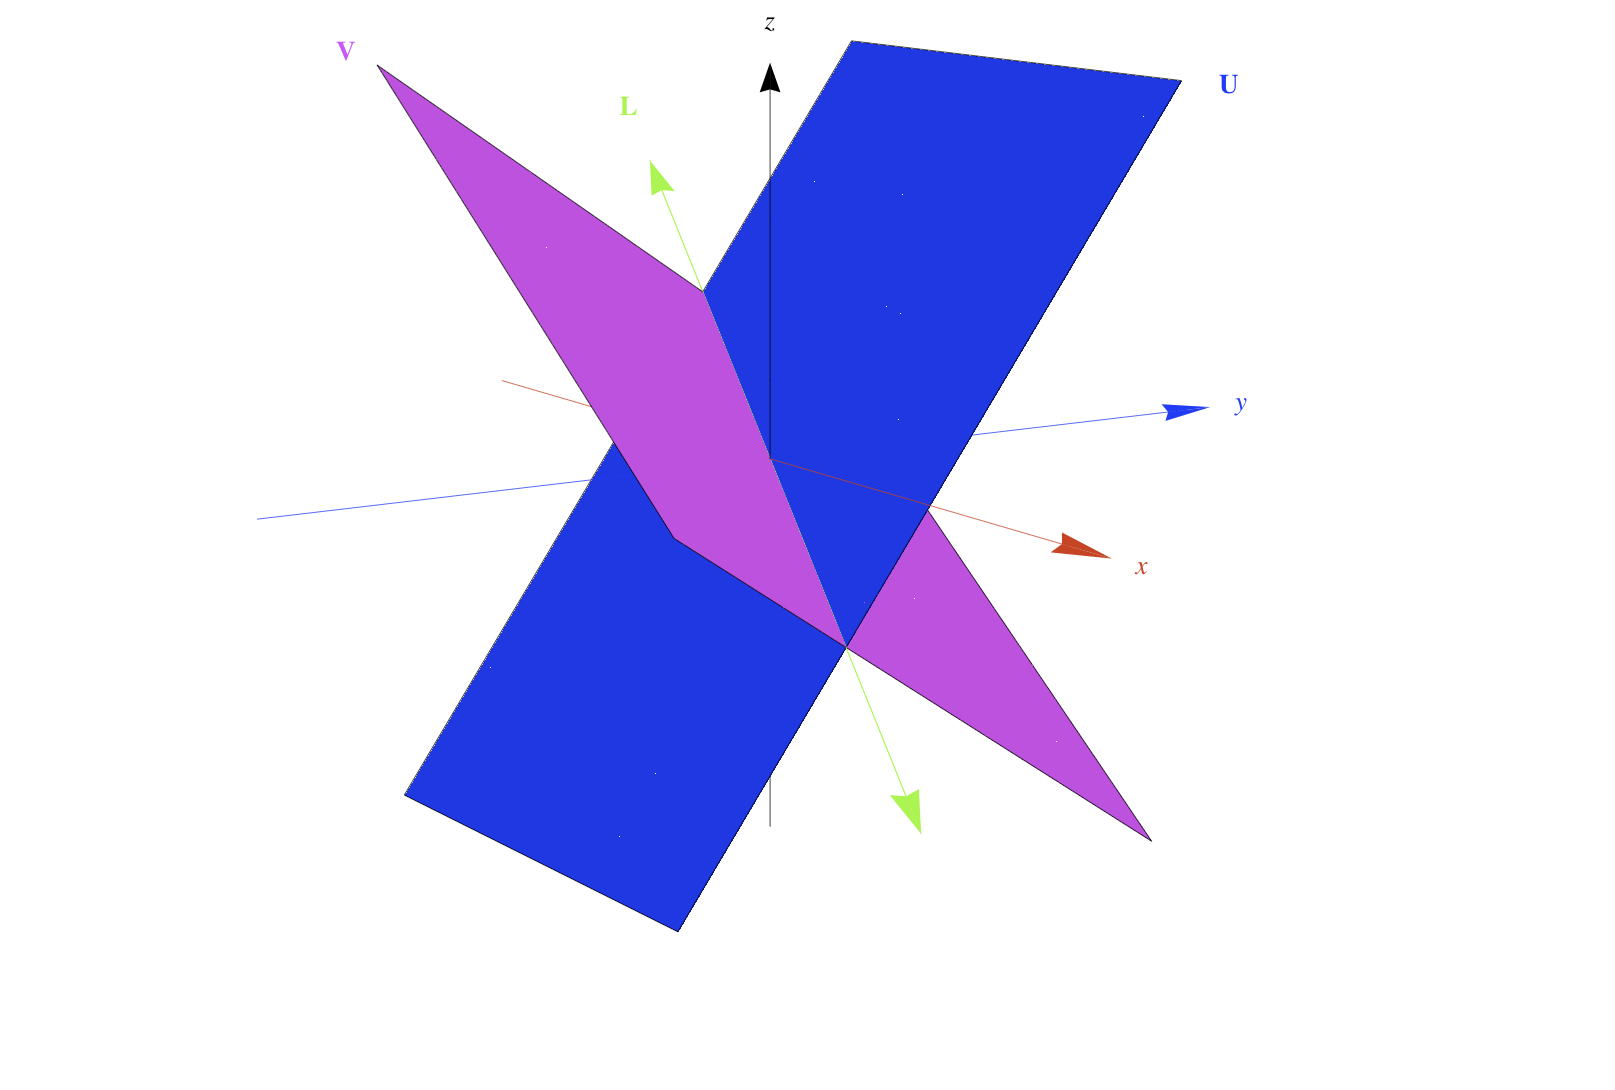
\includegraphics[width=\paperwidth]{img/Planes.jpg}};
\draw (0.5,0.75) node [fill=ocre!30!white,fill opacity=0.6,text opacity=1,inner sep=1cm]{\Huge\centering\bfseries\sffamily\parbox[c][][t]{\paperwidth}{\centering En avant les espaces vectoriels\\[15pt] % Book title
{\Large Une introduction \`a  l'alg\`ebre lin\'eaire (Premi\`ere \'edition)}\\[20pt] % Subtitle
{\small Thierry Giordano, Barry Jessup et Monica Nevins}\\
{\small Traduit en fran\c{c}ais par Abdelkrim El basraoui}}}; % Author name
%\draw[thick,red,->,line width=1cm,] (0,0) -- (0.5,0.5) ;
\end{scope}
\end{tikzpicture}

%\newpage
%
%\begin{tikzpicture}[remember picture,overlay]
%\node[inner sep=0pt] (background) at (current page.north) {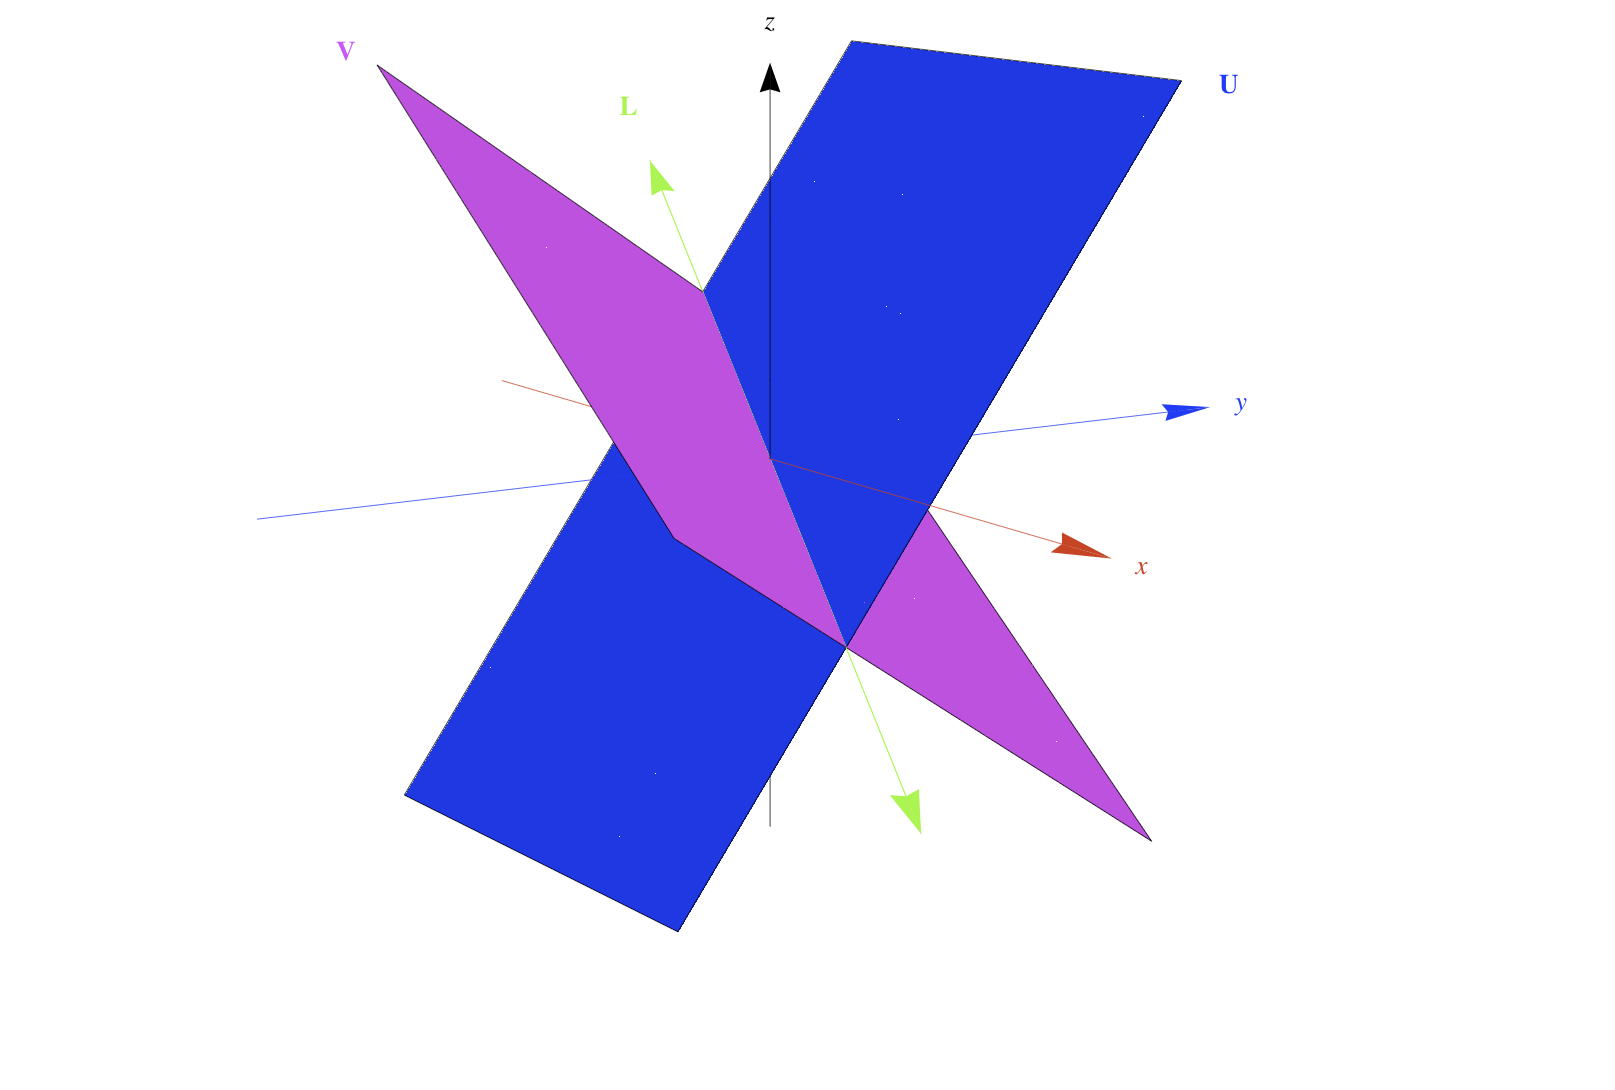
\includegraphics[width=\paperwidth]{img/Planes.jpg}};
%\draw (current page.south) node [fill=ocre!30!white,fill opacity=0.6,text opacity=1,inner sep=1cm]{\Huge\centering\bfseries\sffamily\parbox[c][][t]{\paperwidth}{\centering Vector Spaces First\\[15pt] % Book title
%{\Large An Introduction to Linear Algebra (Fourth edition)}\\[20pt] % Subtitle
%{\small Thierry Giordano, Barry Jessup and Monica Nevins}}}; % Author name
%\end{tikzpicture}
%\vfill
\endgroup

%----------------------------------------------------------------------------------------
%	COPYRIGHT PAGE
%----------------------------------------------------------------------------------------

\newpage
~\vfill
\thispagestyle{empty}



\vspace*{1in}

\noindent \copyright\ \textit{Premi\`ere \'edition fran\c{c}aise, août 2021}\\
\textit{Traduction du livre: \og Vector Spaces First: An Introduction to Linear Algebra\ \fg\ (4th Edition), 2021}


\smallskip
Thierry Giordano, email:
\href{mailto:giordano@uottawa.ca}{giordano@uottawa.ca}



\smallskip
Barry Jessup, email:
\href{mailto:bjessup@uottawa.ca}{bjessup@uottawa.ca}


\smallskip

Monica Nevins, email:
\href{mailto:mnevins@uottawa.ca}{mnevins@uottawa.ca}

\smallskip
Abdelkrim El basraoui, email:
\href{mailto:aelbasra@uottawa.ca}{aelbasra@uottawa.ca}

\smallskip

\noindent \textsc{Ce document est disponible aux endroits suivants:}

\href{https://ruor.uottawa.ca/handle/10393/43430?locale=fr}{https://ruor.uottawa.ca}

\href{https://github.com/uottawa-mathstat/linear-algebra-oer}{https://github.com/uottawa-mathstat/linear-algebra-oer}  \\

%


\noindent 
\includegraphics{copyright.jpg}\\ % URL



\noindent Sauf indication contraire, ce livre est mis à disposition dans le cadre d'une licence Creative Commons de type \href{https://creativecommons.org/licenses/by-nc-sa/4.0/}{Attribution - Pas d’Utilisation Commerciale - Partage dans les Mêmes Conditions 4.0 International (CC BY-NC-SA 4.0)}.  Pour consulter une copie de cette licence, visitez \url{https://creativecommons.org/licenses/by-nc-sa/4.0/}.

Les photos utilisées dans les titres des chapitres sont reproduites avec la permission de l'artiste, Ralph Nevins, \url{ralph.ca}, \href{mailto:ralph@nevins.ca}{ralph@nevins.ca}.


%----------------------------------------------------------------------------------------
%	PREFACE
%----------------------------------------------------------------------------------------

%\usechapterimagefalse % If you don't want to include a chapter image, use this to toggle images off - it can be enabled later with \usechapterimagetrue

\chapterimage{Ottawa3.jpg}
% heading image

%%%%%%%%%%%%%%%%%
%
%%%%%%%%%%%%
%%%%%%%%%%%%%%%%%%%%%%preface.tex%%%%%%%%%%%%%%%%%%%%%%%%%%%%%%%%%%%%%%%%%
% sample preface
%
% Use this file as a template for your own input.
%
%%%%%%%%%%%%%%%%%%%%%%%% Springer %%%%%%%%%%%%%%%%%%%%%%%%%%

\preface

\addcontentsline{toc}{chapter}{Pr\'eface}

Ce volume constitue la traduction fran\c{c}aise de la quatri\`eme \'edition du livre \og Vector Spaces First~\fg\ de Thierry Giordano, Barry Jessup et Monica Nevins, lequel est n\'e de la mise en commun de notes du cours \emph{Introduction à l'algèbre linéaire} enseigné à l'Université d'Ottawa. Ce livre est destiné à servir de manuel ou de compagnon pour compléter le cours.



L'approche que nous adoptons dans ce livre n'est pas standard : contrairement aux approches usuelles, nous introduisons les espaces vectoriels très tôt et nous ne traitons les systèmes linéaires qu'après une telle introduction approfondie des espaces vectoriels.

Nous agissons ainsi pour au moins deux raisons. D'une part, après avoir enseigné ce cours de diverses manières à plusieurs milliers d'étudiants sur près de vingt-cinq ans, nous sommes maintenant en mesure d'observer que les outils relatifs aux espaces vectoriels sont généralement mal vécus par les étudiants car ils représentent la partie la plus difficile du cours et trouvent pourtant traditionnellement leur place à la fin. Dans un cours dispensé en seulement douze semaines, le fait que la matière la plus difficile se trouve à la fin ne laisse pas à la plupart des étudiants suffisamment de temps pour s'attaquer aux concepts (apparemment) nouveaux que l'on peut rencontrer lorsque l'on s'attaque aux espaces vectoriels pour la première fois.

À l'opposé, notre expérience nous montre que le fait d'aborder les espaces vectoriels dès les deux premières semaines permet aux étudiants de bien mieux appréhender les deux \og grandes~\fg\ idées de l'algèbre linéaire: la notion de combinaison linéaire d'une famille de vecteurs, qui donne lieu à ce que l'on appelle \og enveloppe lin\'eaire~\fg, et la notion d'\og indépendance linéaire~\fg\ d'une famille de vecteurs. Ces deux notions sont au cœur de l'algèbre linéaire et sont généralement ressenties comme nouvelles, abstraites et difficiles par les étudiants lorsqu'elles sont rencontrées pour la première fois. Le mieux est donc sans doute d'introduire ces notions le plus tôt possible pour pouvoir ensuite les utiliser et ainsi définir par exemple les notions de {\it base} et de {\it dimension}, lesquelles sont utiles à la fois dans le reste du cours et dans différents autres contextes. Aussi, toujours d'après notre expérience, la plupart des étudiants semblent préférer aborder les concepts difficiles le plus tôt possible afin d'avoir le temps de se familiariser avec des idées vraisemblablement nouvelles et différentes de ce qu'ils avaient vu dans l'enseignement secondaire.

D'autre part, une autre raison justifiant notre organisation est d'alerter les étudiants sur le fait qu'il y a réellement des concepts à la fois nouveaux et différents dans ce cours ! En effet, si l'on commençait le cours avec les systèmes linéaires que beaucoup d'étudiants ont déjà étudiés auparavant (en petite dimension du moins), il serait alors facile de se reposer sur l'idée qu'au final peu de nouvelles notions seront abordées dans ce cours, si bien que les étudiants seraient pris au dépourvu plus tard lorsque les espaces vectoriels sont introduits... Au contraire, si l'on commence avec des concepts nouveaux mais abordables, les étudiants sont stimulés pour aller de l'avant. D'où notre choix d'organisation pour cet ouvrage.








%----------------------------------------------------------------------------------------
%	Acknowledgements
%----------------------------------------------------------------------------------------

\chapterimage{Delta2.jpg}
%%%%%%%%%%%%%%%%%
%
%%%%%%%%%%%%
\chapter*{Remerciements}

\section*{Remerciements des auteurs de la version anglaise}
Les auteurs tiennent à remercier toutes celles et ceux qui ont contribué à la réalisation de ce livre, consciemment ou non. Ce livre est en quelque sorte la compilation de diverses notes pour un cours qui était destiné à des élèves de première année à l'Université d'Ottawa. Sur cette longue période d'enseignement, les auteurs ont été influencés par plusieurs manuels aussi excellents et complets les uns que les autres, comme ceux de Howard Anton, W. Keith Nicholson, David C. Lay, Seymour Lipschutz ou encore Marc Lipson (voir les références à la fin de l'ouvrage). Au fil des années, les auteurs ont également consulté les ouvrages de Tom M. Apostol, Otto Brestcher et Gilbert Strang.


Les auteurs expriment leur gratitude envers leurs collègues qui ont su déceler les inévitables et innombrables erreurs de la première édition. Ils remercient tout particulièrement Anne Broadbent, Saeid Molladavoudi ainsi que Charles Starling qui ont non seulement dressé des listes d'erreurs, mais aussi suggéré d'excellentes modifications.

Ce livre a été utilisé pour la première fois comme manuel de cours à l'automne 2015. Les auteurs sont reconnaissants envers les dizaines d'étudiants de la section MAT1341 qui ont lu le livre et qui ont eu la bienveillance de faire savoir les erreurs qu'ils rencontraient.

Ceci étant dit, les erreurs qui subsistent encore malgré tout sont entièrement dues aux auteurs !
{\flushright

Thierry Giordano, Barry Jessup \& Monica Nevins



Janvier 2015



Universit\'e d'Ottawa

}

\section*{Remerciements de l'auteur de la version fran\c{c}aise}

Je tiens \`a remercier toutes celles et ceux qui ont contribu\'e \`a la naissance de cette premi\`ere version fran\c{c}aise. En particulier, je remercie Anne Broadbent pour tout le travail qui ne se limite pas uniquement au lancement et \`a la r\'ealisation de ce projet, mais qui est aussi allé plus en profondeur.
Un remerciement spécial doit aussi être accordé \`a Monica Nevins pour son soutient, ses commentaires et surtout la mise en page de ce livre. Des remerciements se doivent aussi \`a Tanya Schmah pour la mise \`a notre disposition de l'outil \og Polymath~\fg\ et les efforts fournis pour la traduction. Je remercie également Ralph Nevins pour les photos mises \`a notre disposition.
J'aimerais \'egalement faire part de ma gratitude envers les concepteurs de \og \url{deepl.com}~\fg\ pour la version gratuite qu'ils ont mis à notre disposition.
Anne et moi aimerions également remercier l’Université d’Ottawa qui a soutenu ce projet de traduction par l’entremise du programme de subvention pour les Ressources Éducatives Libres (REL), et particuli\`erement Mme Mélanie Brunet pour son support et son accompagnement. 
Je me joins \`a Anne et Monica pour remercier chaleureusement Pierre Botteron pour la relecture et correction tr\`es attentive de cette version. 
Enfin, je tiens \`a remercier les membres de ma petite famille pour leur patience et leur soutien lors de la r\'ealisation de ce projet.

\vspace{10mm}

{\flushright

Version fran\c{c}aise: Abdelkrim El basraoui




Ao\^ut 2021



Universit\'e d'Ottawa

} 

%----------------------------------------------------------------------------------------
%	TABLE OF CONTENTS
%----------------------------------------------------------------------------------------

\chapterimage{Rockies.jpg}

\pagestyle{empty} % Disable headers and footers for the following pages

\tableofcontents % Print the table of contents itself

\cleardoublepage % Forces the first chapter to start on an odd page so it's on the right side of the book

\pagestyle{fancy} % Enable headers and footers again


%----------------------------------------------------------------------------------------
%	List of acronyms
%----------------------------------------------------------------------------------------

\chapterimage{Ottawa4.jpg}
%%%%%%%%%%%%%%%%%%%%%%acronym.tex%%%%%%%%%%%%%%%%%%%%%%%%%%%%%%%%%%%%%%%%%
% sample list of acronyms
%
% Use this file as a template for your own input.
%
%%%%%%%%%%%%%%%%%%%%%%%% Springer %%%%%%%%%%%%%%%%%%%%%%%%%%

\extrachap{Acronymes}

\addcontentsline{toc}{chapter}{Acronymes}

\index{acronymes, liste d'} \index{symboles, liste de} 

\paragraph{Abréviations courantes utilisées dans ce livre}

\begin{tabular}{ll}
	$\col(A)$ & {l'espace des colonnes de la matrice $A$} \\
	$\row(A)$ & {l'espace des lignes de la matrice $A$} \\
	$\im(T)$ & {l'image de la transformation linéaire $T$} \\
	$\ker$&  {le noyau (d'une matrice ou d'une transformation linéaire)} \\
	$\det$& {le d\'eterminant (d'une matrice)} \\
	$\tr$& {la trace (d'une matrice)} \\
	$\sp~$& {l'enveloppe lin\'eaire (engendr\'ee par un ensemble de vecteurs)} \\
	LD& {Linéairement Dépendant} \\
	LI&{Linéairement Indépendant} \\
	ME&{Matrice \'Echelonn\'ee } \\
	MER&{Matrice \'Echelonn\'ee R\'eduite}
\end{tabular}

\paragraph{Symboles communs}

\begin{tabular}{ll}
	$V$ &{un espace vectoriel} \\
	$U$ & {un sous-espace vectoriel de $V$} \\
	$\vv$& {un vecteur} \\
	$\zero$& {le vecteur nul} \\
	$A^T$& {la transpos\'ee de la matrice $A$} \\
	$A^{-1}$& {l'inverse de la matrice $A$}
\end{tabular}


%%%%----------------------------------------------------------------------------------------
%%%%	PART I : Algebra and Geometry
%%%%----------------------------------------------------------------------------------------
\chapterimage{Ottawa1.jpg} % Table of contents heading image
%Ottawa1933

\renewcommand{\partintrotext}{L'un des principaux thèmes de l'algèbre linéaire est la généralisation des idées de la géométrie à des dimensions supérieures, en interprétant les idées géométriques de manière algébrique. Réciproquement, on peut aussi voir qu'aborder un problème algébrique avec un point de vue géométrique donne du recule sur les questions algébriques.

\medskip

Nous commençons notre exploration de ces thèmes par l'étude des nombres complexes, puis par une révision de la géométrie vectorielle (dans l'optique d'étendre certaines idées aux dimensions supérieures).}

\part{Alg\`ebre et g\'eom\'etrie}



\chapter{Nombres complexes}

\label{chapter:Fr_01-Complex}



Pour faire court, on pourrait dire que l'algèbre est l'étude des solutions d'équations polynomiales.
Par exemple, l'algèbre \emph{linéaire} est une branche de l'algèbre qui se consacre à l'étude des solutions d'équations \emph{linéaires}. (Cette branche de l'algèbre est particulièrement intéressante lorsque l'on utilise de nombreuses variables et équations, ce que nous ferons dans le Chapitre~\href{chapter:11-solvingsystems}).



Dans le chapitre d'aujourd'hui, intéressons-nous à une conséquence fameuse de l'algèbre pour se \og remettre en jambes \fg~après un long été de vacances : les nombres complexes. C'est un incontournable pour nos chers ingénieurs (particulièrement en génie électrique) et nos chers physiciens qui vont très bientôt les utiliser à longueur de journée.


\section{Définition des nombres complexes}

L'histoire des nombres complexes est très intéressante. Elle ne commence pas comme on pourrait le croire avec la fameuse équation
$$
x^2 + 1 = 0,
$$ mais plutôt avec des équations cubiques (qui font intervenir des termes en $x^3$) !
À l'époque, tout le monde était certain que  l'équation $ x^2 + 1 = 0$
n'a pas de solution---il suffit de regarder le graphe de la fonction $y=x^2+1$ et de voir qu'il ne croise pas l'axe des abscisses. \footnote{De même, encore avant, on aurait dit que l'équation $x+1=0$ n'a pas de solution non plus puisque les nombres négatifs ne représentent pas une quantité mesurable dans la vie de tous les jours et que donc ils « n'existaient pas ».} Cependant, en se basant sur la remarque que chaque équation \emph{cubique} avec coefficients réels admet au moins une solution réelle, les nombres imaginaires (aussi longtemps appelés « nombres sophistiqués » par le mathématicien Jérôme Cardan) ont été introduits pour obtenir une formule décrivant ces solutions réelles.\footnote{Pour plus de détails, cherchez sur le web « histoire des nombres complexes ».} 


Ceci étant dit, revenons à la notation de $i$ comme étant une solution de l'équation $  x^2 + 1 = 0$;  « i » pour « imaginaire » (notation due à Euler, 1777). Alors :
\[ i^2 = -1 \qquad \text{ou bien} \qquad i = \sqrt{-1}, \]
et avec ceci nous définissons la racine carrée d'un nombre réel \emph{négatif} $a$ par
$$\sqrt{a}:=(\sqrt{\vert a\vert}) i.$$

Cela peut sembler fastidieux! En fait, si nous appliquons les règles de l'algèbre, comme dans
$$
\sqrt{-9} = \sqrt{9 \cdot (-1)} = \sqrt{9} \cdot \sqrt{-1} = 3i,
$$ nous obtenons la bonne réponse, $\sqrt{-9}=3i$, mais il faut faire très attention à la troisième égalité.
\footnote{Un vrai cours d'analyse complexe est nécessaire ici car sinon on peut avoir des problèmes, comme par exemple la contradiction $9=\sqrt{81}=\sqrt{(-9)(-9)}\not=\sqrt{ -9 }\  \sqrt{ -9 }=3i\, 3i =-9$... En effet, la règle pour les nombres réels positifs $a,\  b$ qui énonce (correctement) que : $\sqrt{ab}=\sqrt{a}\,\sqrt{b}$ \emph{n'est pas valable} en général pour les réels négatifs. Ceci peut sembler être une nuisance, mais c'est en fait la source de beaucoup de découvertes mathématiques intéressantes. Cherchez sur le web « surface de Riemann et racine carrée ».}  Contentez-vous de cette définition fastidieuse pour le moment!

(Toutefois, veuillez noter que comme en arithmétique, nous adhérons à la convention $\sqrt{a^2} =\vert a \vert$ peu importe si $a$ est positif ou négatif. En d'autres termes, quand on calcule la racine carré $\sqrt{b}$ d'un nombre réel positif $b$, la réponse à donner est l'unique
valeur positive $c$ telle que $c^2=b$, même si on aurait pu aussi prendre $c$ négative.)



Cependant, le nouveau nombre $i$ en tant que tel n'est pas tout à fait suffisant! Il va falloir qu'on puisse multiplier $i$ avec un nombre réel et y ajouter un nombre réel. En effet par exemple, considérons l'équation
$$
x^2 + 4x + 8 = 0.
$$
Par la formule quadratique, cette équation donne les deux racines suivantes :
$$
x = \frac{-4 \pm \sqrt{16-32}}{2} = -2 \pm \frac12 \sqrt{-16} = -2 \pm \frac12 (4i) = -2 \pm 2i,
$$
où nous avons simplifié $\sqrt{-16}$ grâce à la définition « fastidieuse » introduite précédemment.
Vérifions que ces racines ont bien un sens. Substituons d'abord $x = (-2+2i)$ dans l'équation quadratique et simplifions :
$$
(-2+2i)^2 + 4(-2+2i) + 8 = (4 -4i - 4i + 4i^2) + (-8 +8i) +8 = 4+4i^2 = 0\,,
$$
où dans la dernière étape nous appliquons $i^2 = -1$. On obtient donc bien $0$. De même, nous
pouvons vérifier que $-2-2i$ est aussi racine de l'équation.




Ayant cette remarque à l'esprit ainsi que la formule quadratique
, nous arrivons à la définition suivante.

\begin{definition}
L'ensemble des \emph{nombres complexes} est l'ensemble
$$
\C = \{ a+b\,i \colon a, b \in \mathbb{R} \}.
$$
\noindent(\`A interpréter comme:  « l'ensemble de tous les objets de la forme $a+bi$, où $a$ et
$b$ sont des nombres réels »).

Lorsque l'on écrit
$$
z =a +b\,i \in \C,
$$
on veut dire  $z$ (ou $a+b\,i $) appartient à $\C $.\\
\indent Terminologie:
$a$ est appelé la \emph{partie réelle} de $z$ (notée $Re(z)$) et $b$ est appelé
la partie imaginaire de $z$ (notée $Im(z)$).  Notez que $Re(z)$ et $Im(z)$ sont des nombres \emph{réels} !


Lorsque $Re(z)=0$, alors $z=bi $ et nous dirons que $z $ est un \emph{imaginaire pur}; et
quand $Im(z)=0$, alors $z=a$ et on dit que $z$ est un \emph{réel pur}.  Ainsi $\R \subset \C$, ce qui se lit :  $\R$
est un sous-ensemble de $\C$.

\end{definition}

De même que les nombres réels sont représentés sur une droite, la droite des nombres réels, les nombres complexes sont représentés dans un plan, 
le \emph{plan complexe}, que nous étudierons bientôt.

Rappelez-vous bien que, pour toute équation quadratique $ax^2+bx+c=0$ dont les coefficients $a,\, b,\, c$ sont réels, les racines sont de la forme $$x = \frac{-b}{2a} \pm \frac{\sqrt{b^2-4ac}}{2a}. $$ Si $b^2-4ac \geq 0$, les racines sont (purement) réelles. Sinon, elles sont des nombres complexes.  Donc au final, TOUTES les équations quadratiques admettent DEUX racines (en adoptant la convention qu'une racine double est comptée comme deux racines à partir de maintenant).

\section{Algèbre des nombres complexes}

\begin{itemize}
\item Égalité: $a+bi = c+di \Leftrightarrow\,  a=c\, \textrm{ et }\, b=d$.
\item Addition : $(a+bi) + (c+di) = (a+c) + (b+d)i$.
\item Multiplication : $(a+bi)(c+di) = (ac-bd) + (ad+bc)i$.
\end{itemize}

En fait, les nombres complexes satisfont les mêmes propriétés 
que les nombres réels, sauf qu'il n'y a pas de relation d'ordre (c'est-à-dire que l'expression « $z>y$ » n'a pas de sens avec les nombres complexes).

{\bf Question:} Qu'en est-il de la division ?

\begin{myexample}
Essayons de résoudre l'équation $(4+3i)z = 1$, si possible. Autrement dit, qu'entendons-nous par la fraction suivante : 
$$
z = \frac{1}{4+3i} \,?
$$
(SVP SVP rappelez-vous que par exemple $\frac{1}{2+3} \neq \frac12 + \frac13$ !!!)


\begin{mysol}
Idée : rappelez-vous que $i$ est une racine carrée puis utilisez le processus standard de l'algèbre appelée \emph{rationalisation du dénominateur}.

Remarquez que
 $$(a+b \, i)(a-b\, i) = a^2-(b\, i)^2 = a^2+b^2,$$ et comme $a$ et $b$ sont \emph{réels}, on a $a^2+ b^2 \neq 0$
sauf si $a$ et $b$ sont tous les deux nuls.

En considérant le nombre complexe $z=a+bi$ avec $a,\, b\in\R$, on définit :
\begin{itemize}
\item $\overline{z} = a-bi$ s'appelle le \emph{conjugué} (complexe) de $z$. Notez que nous avons en fait déjà utilisé des conjugués complexes dans la formule quadratique. Essentiellement, l'idée pour calculer $\overline{z}$ à partir de $z$ est de remplacer « $ i $ » par « $ -i $ », et il n'est même pas nécessaire d'avoir simplifié l'expression de $z$ au préalable avant de faire un tel remplacement.
\item $| z | = \sqrt{a^2+b^2}$ s'appelle le \emph{module} de $z$. Contrairement à $z$ qui est un nombre complexe, son module $|z|$ est un nombre réel.
\item La forme $z=a+bi$, où $a,\, b\in\R$, s'appelle la \emph{forme cartésienne} de $z$. On verra plus tard d'autres formes pour écrire un nombre complexe.
\end{itemize}

Soulignons que l'égalité
$z = 0$ est vraie si et seulement si (ssi) $\vert z \vert = 0$, et contrairement aux nombres complexes, nous POUVONS toujours
comparer le module des nombres complexes : par exemple $\vert i \vert =  1 > 0 =  \vert 0 \vert$; ceci est vrai car, comme on l'a dit, le module $|z|$ est toujours un nombre réel.

Maintenant que nous avons rappelé les notions de conjugué et de module d'un nombre complexe, on peut s'intéresser à l'expression suivante :
$$
z \overline{z} = \vert z \vert^2 = \vert \overline{z} \vert^2,
$$
laquelle donne
$$
z \cdot \left(\frac{\overline{z}}{\vert z \vert^2}\right) = 1
$$
ou encore
$$
\frac{1}{z} = \frac{\overline{z}}{\vert z \vert^2}.
$$

Ainsi, dans notre exemple, on obtient finalement :
$$
\frac{1}{4+3i} = \left(\frac{1}{4+3i} \right) \left( \frac{4-3i}{4-3i} \right) = \frac{4-3i}{4^2+3^2} = \frac{4-3i}{25} = \frac{4}{25} - \frac{3}{25}i.
$$
\end{mysol}
\end{myexample}

\begin{myprob}
Écrire sous forme cartésienne $a+b\,i$ le nombre complexe suivant :
$$
\frac{3+2i}{-2+4i}\, .
$$

\begin{mysol}
Multipliez par $1 = \frac{-2-4i}{-2-4i}$ puis simplifiez comme suit :
$$
\frac{3+2i}{-2 + 4i} = \frac{3+2i}{-2 + 4i}\cdot \frac{-2-4i}{-2-4i} =
\frac{(3+2i)(-2-4i)}{4+8i-8i-16i^2} = \frac{2-16i}{20} = \frac{1}{10} - \frac{4}{5}i.
$$
Ainsi, il suffit de prendre $a=\frac{1}{10}$ et $b=-\frac45$.
\end{mysol}
\end{myprob}

Voici d'autres propriétés faciles à démontrer.

\begin{lemma}[Propriétés des nombres complexes]
 Pour
$z,w \in \C$ et $c\in \R$, on a:
\begin{enumerate}
\item $\frac{1}{z} = \frac{\overline{z}}{\vert z \vert^2}$;\smallskip
\item $\overline{z+w} = \overline{z} + \overline{w}$;
\item $\overline{cz} = c\overline{z}$;
\item $\overline{zw} =\overline{z}\; \overline{w}$;
\item $\overline{z/w} = \overline{z}/\overline{w}$.\smallskip
\item $\overline{\overline{z}} = z$  (e.g. : $\overline{\overline{3+2i}}= \overline{3-2i} = 3+2i$);
\item $\overline{z} = z$ ssi $z \in \R$;
\item $\overline{z} = -z$ ssi $z$ est un imaginaire pur;
\item $\vert z \vert  \in \R$ et $\vert z \vert \geq 0$;
\item $\vert z \vert = \vert \overline{z} \vert$;
\item $\vert zw \vert = \vert z \vert \, \vert w \vert$;
\item $\vert z/w \vert = \vert z \vert / \vert w \vert$;
\item $\vert z + w \vert \leq \vert z \vert + \vert w \vert$ (« Inégalité triangulaire »);
\item Si $a$ est un nombre réel, alors $\vert a + 0i \vert$ est la valeur absolue de $a$.
  (On écrit simplement $z=a$ plutôt que $z=a+0i$).
\end{enumerate}


\end{lemma}

\begin{proof}
Nous prouvons ici deux de ces propriétés et nous laissons les autres en exercice aux soins du lecteur.
(Conseils : pour l'inégalité triangulaire, une astuce est d'utiliser la géométrie des nombres complexes, cf. section 1.3. Pour les propriétés avec des multiplications de nombres complexes, il est plus simple d'utiliser la forme polaire, cf. sections 1.4 et 1.5).

\begin{enumerate}
	\item[2.] Supposons que $z$ et $w$ sont des nombres complexes.
Alors $z$ s'écrit
$z = a+bi$ pour certains nombres réels $a$ et $b$, et $w = c+di$
pour certains nombres réels $c$ et $d$.

D'une part, on a $z+w = (a+c) + (b+d)i$ et donc $$\overline{z+w} = (a+c) - (b+d)i.$$

D'autre part, on a $\overline{z} = a-bi$ et $\overline{w} = c-di$, ce qui donne
$$\overline{z} + \overline{w} = (a+c)+(-b-d)i = (a+c)-(b+d)i.$$

Les deux côtés sont donc égaux, ce qui complète la preuve.


	\item[10.] Supposons que $z$ est un nombre complexe.  Comme
$
\vert z \vert = \sqrt{z \overline{z}},
$
on a
$$
\vert \overline{z} \vert = \sqrt{\overline{z} \ \overline{\overline{z}}}  = \sqrt{\overline{z} z }= \sqrt{ z \overline{z} }= \vert z \vert.
$$
CQFD.
\end{enumerate}
\end{proof}


\section{Géométrie des nombres complexes}

\begin{center}
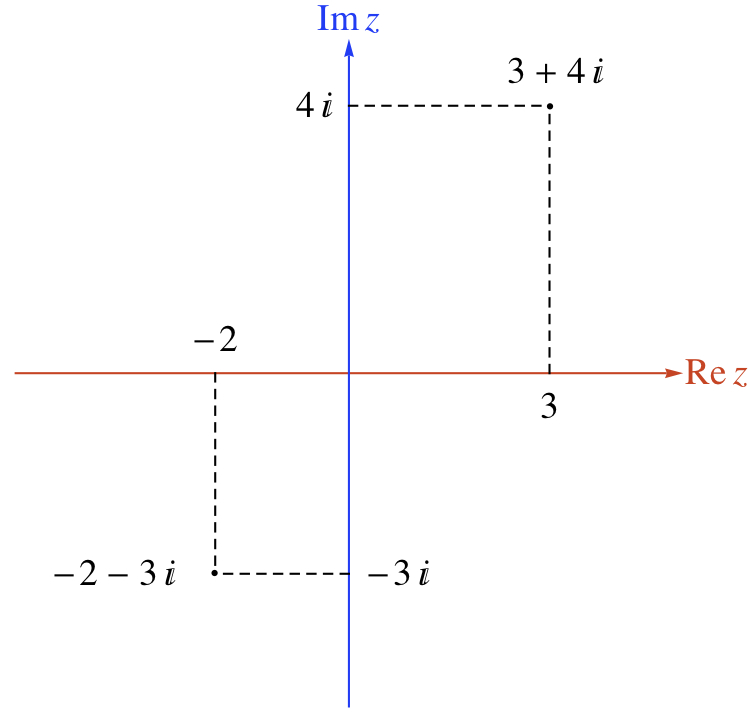
\includegraphics[scale=.4]{complexplane.jpg}~\\[1cm]
\end{center}
Chaque nombre complexe $z$
peut s'écrire de manière unique sous la forme $z=a+b\,i$ pour certains nombres réels $a$ et $b$. Pour représenter $z$ dans un graphique,
on lui associe le point de coordonnées $(a,b)$ dans le plan $xy$.
Ainsi $z=a+b\,i$ est vu comme un point du plan $xy$, et nous appellerons donc ce plan le \emph{plan complexe}.  L'axe horizontal est appelé
l'\emph{axe réel} et l'axe vertical
est appelé l'\emph{axe imaginaire}.



L'addition de deux nombres complexes est la même que l'addition de
deux vecteurs dans le plan.  L'opposé $-z$ d'un nombre complexe $z$ correspond au vecteur opposé du vecteur lié à $z$, comme représenté sur le dessin ci-dessus.  La multiplication
par un nombre réel est simplement la multiplication scalaire d'un vecteur, mais la multiplication
par un nombre complexe est plus subtile : c'est en fait une combinaison de rotation et d'homothétie.
(Essayez de faire les calculs pour voir ce que ça donne !)

Le conjugué complexe $\overline{z}$ correspond juste la symétrie par rapport à l'axe réel.  Ainsi, les nombres complexes $z = a+b\,i$ et $\overline{z} = a-b\,i$ ont la même abscisse mais leurs ordonnées sont opposées.

Le module $|z|$ de $z$ est simplement la longueur du vecteur représentant $z$.
(Rappelons que la formule de la longueur du vecteur de coordonnées $(a,b)$ est simplement
$\sqrt{a^2+b^2}$. )

\section{Forme polaire d'un nombre complexe}


Dans cette section nous ré-écrirons les nombres complexes sous une nouvelle forme, la \emph{forme polaire} $z= r\, e^{i\, \theta}$. Notez que les coordonnées $(r,\theta)$ sont aussi appelées « coordonnées polaires » dans le cas du plan réel $\mathbb R^2$, cf. les cours Calcul II et Calcul III.


 \begin{center}
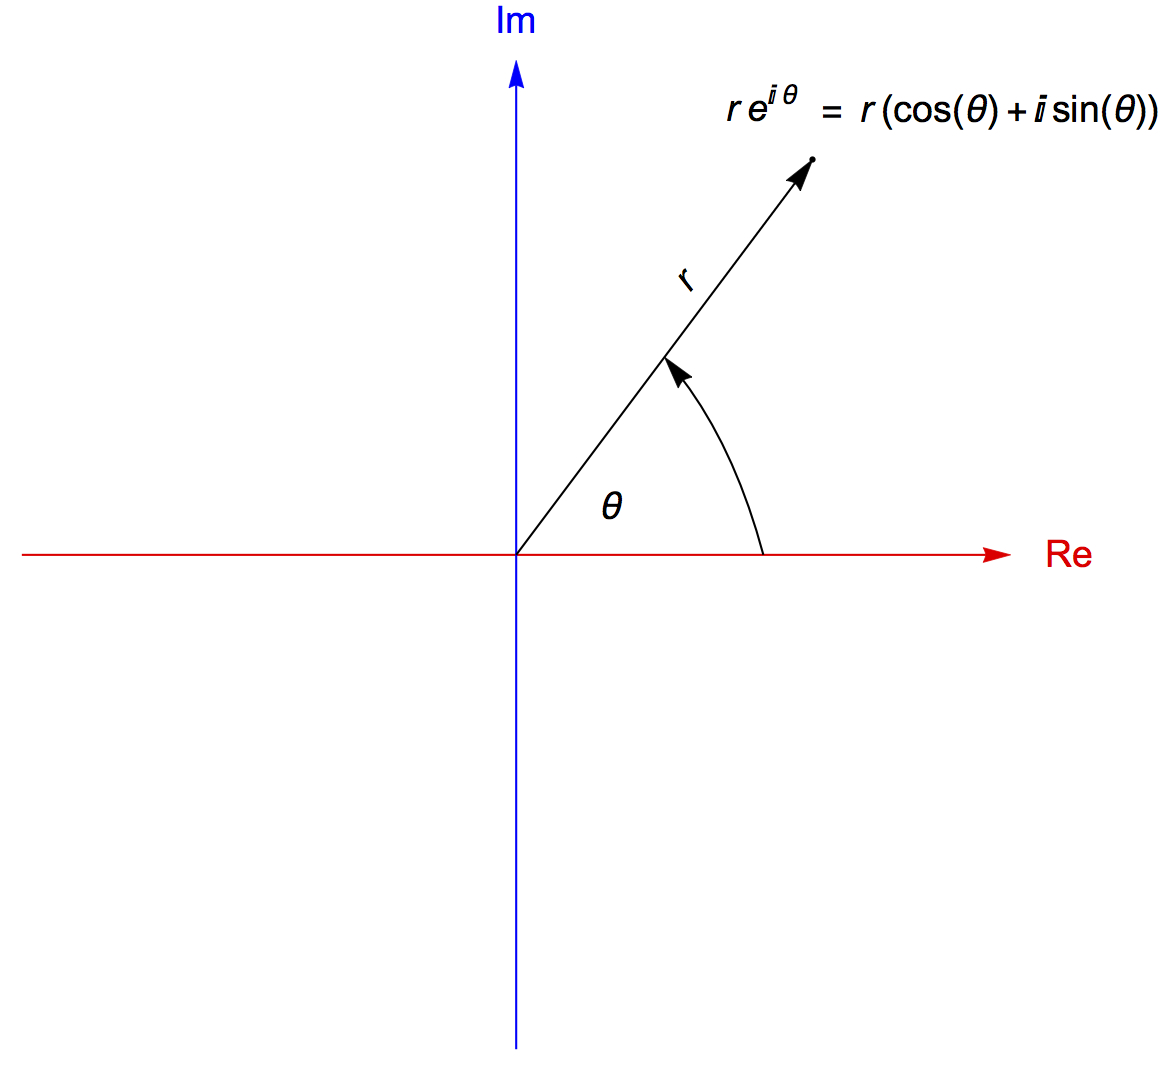
\includegraphics[scale=.4]{PolarForm.jpg}~\\[1cm]
\end{center}




Si $z = x+y\,i \in \C$ est non-nul, alors on définit 
$$
r = \vert z \vert = \sqrt{x^2+y^2} \neq 0,
$$
et par les formules trigonométriques, on a :
$$
\frac{x}{r} = \cos(\theta), \qquad \frac{y}{r} = \sin(\theta).
$$
Par conséquent, on peut écrire
$$
z = x+yi = r \cos(\theta) + i r\sin(\theta) = r(\cos(\theta)+i \sin(\theta)).
$$

L'angle $\theta$ est noté $\theta = arg(z)$ et s'appelle \emph{argument} de $z$. Remarquez que $\theta$ n'est pas déterminé de fa\c{c}on unique
puisque n'importe quel $\theta' = \theta + 2n\pi$ avec $n\in \Z$ fonctionne aussi.  C'est pour cela qu'en général nous
choisirons $\theta$ tel que $-\pi < \theta \leq \pi$, qui lui par contre est unique, que nous noterons $\theta = Arg(z)$ et que nous appellerons l'\emph{argument principal} de $z$.

En 1748, Euler a démontré que

$$
e^z = 1 + z + \frac{z^2}{2} + \cdots = \sum_{n=0}^\infty \frac{z^n}{n!}.
$$
(C'est ce qu'on appelle généralement \emph{série entière}). De manière surprenante, en comparant les séries entières avec les fonctions trigonométriques,
on obtient la formule élégante :
$$
e^{i\theta} = \cos(\theta) + i\sin(\theta).
$$
La notation moderne de la \emph{forme polaire} du nombre complexe $z$ est donc simplement :
$$
z = r \,e^{i\theta}.
$$

\begin{myexample} \label{ex: calculer quelques formes polaires}
À partir du diagramme ci-dessous, vérifiez que $2i= 2\,e^{i \frac{\pi}2}$, $-i=e^{-i \frac{\pi}2}$, $-1 = e^{i\pi}$ et
$1+i =\sqrt{2}\,e^{i \frac{\pi}4}$.
\end{myexample}
\begin{center}
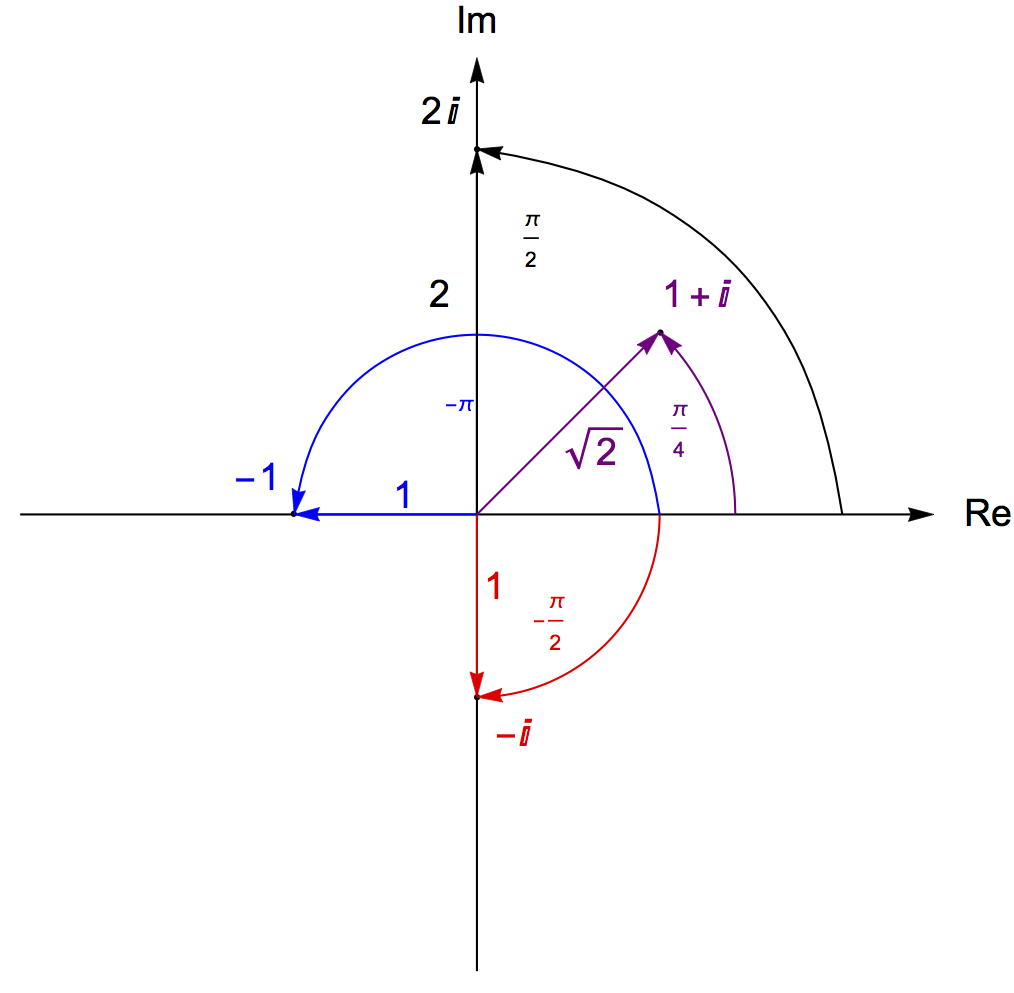
\includegraphics[scale=.4]{PolarFormExample.jpg}~\\[1cm]
\end{center}


Notez que nous avons également les propriétés suivantes :
\begin{itemize}
\item $re^{i\theta} = r' e^{i\theta'}$ ssi $r=r'$ et $\theta = \theta' + 2n\pi$ pour un certain $n\in \Z$;
\item $\overline{re^{i\theta}} = re^{-i\theta}$;
\item $\vert e^{i\theta} \vert = 1$ pour tout $\theta\in\R$.
\end{itemize}

\section{Multiplication de nombres complexes sous forme polaire}

Soient $z = re^{i\theta}$ et $w = se^{i\phi}$. Alors
\begin{align*}
zw &= \left( r(\cos(\theta)+i\sin(\theta)) \right) \left(s (\cos(\phi)+i\sin(\phi)\right) \\
&= (rs)\left( (\cos(\theta)\cos(\phi) - \sin(\theta)\sin(\phi)) + i(\cos(\theta)\sin(\phi) + \sin(\theta)\cos(\phi)) \right)\\
&= rs\,(\cos(\theta + \phi) + i\sin(\theta + \phi))\\
&= rs\,e^{i(\theta+\phi)}.
\end{align*}
On se retrouve donc avec la formule habituelle de la multiplication avec des exposants.  (Idem pour la
division, on retrouve la formule habituelle.)

\begin{myprob}
Écrire sous forme polaire le nombre complexe suivant : 
$$
\frac{i}{1+i}\, .
$$

\begin{mysol}
D'après l'exemple \ref{ex: calculer quelques formes polaires}, nous avons $i = e^{i\frac{\pi}{2}}$ et
$1+i = \sqrt{2}\,e^{i\frac{\pi}{4}}$.
Donc
$$
\frac{i}{1+i} = \frac{e^{i\frac{\pi}{2}}}{\sqrt{2}\,e^{i\frac{\pi}{4}}}
 = \frac{1}{\sqrt{2}}\,e^{i\frac{\pi}{4}}\, .
$$
(Vérifiez aussi ceci en utilisant la première méthode avec la forme cartésienne, et vous verrez quelle est un peu plus lente que la nouvelle méthode.)
\end{mysol}
\end{myprob}

\section{Le Théorème fondamental de l'algèbre}



Nous avons déjà vu que toute équation quadratique à coefficients réels admet deux racines complexes. Remarquez d'ailleurs que si l'une des deux racines $z$ n'est pas réelle, alors l'autre non plus n'est pas réelle car elle correspond au complexe conjugué $\overline{z}$. 

Inversement, étant donné un nombre complexe $z$, on peut toujours trouver un polynôme à coefficients réels dont les
racines sont exactement $z$ et $\overline{z}$ :
$$
(x-z)(x-\overline{z}) = x^2 -(z+\overline{z})x + z \overline{z}.
$$
Heu... mais est-ce que les coefficients de ce polynôme sont vraiment réels ?  HÉ OUI !  Écrivez
$z = a+ib$; alors $z+\overline{z} = 2a$ est réel, et
$z \overline{z} = |z|^2$ aussi comme nous l'avons prouvé précédemment.

En résumé, tout polynôme à coefficients réels admet au moins une racine complexe (lorsque bien sûr le polynôme n'est pas constant...), et tout nombre complexe est racine d'au moins un certain polynôme à coefficients réels.

Notez toutefois que si vous prenez deux nombres complexes $z$ et $w$ qui ne sont pas conjugués, alors le polynôme $(x-z)(x-w)$ n'est pas forcément à coefficients réels, il est en général à coefficients complexes...
Ceci nous amène à la question suivante : si vous prenez une équation quadratique
à coefficients complexes et que vous utilisez la formule quadratique pour
pour la résoudre, de quels nombres supplémentaires (comme $i$) aurez-vous besoin ?

Réponse : en fait, comme l'énonce le théorème suivant, AUCUN !  Les nombres complexes sont tellement généraux qu'ils englobent tout ce dont vous aurez besoin à jamais (ou du moins pour très longtemps) ! C'est ça qui fait le vrai intérêt des nombres complexes.

\begin{theorem} [Théorème fondamental de l'algèbre] \label{theoreme : theoreme fondamental de l algebre}
Tout polynôme à coefficients dans $\C$
se factorise complètement en facteurs simples de la forme $ax+b$,
avec $a,\, b \in \C$.
\end{theorem}

\section[Réflexions sur le Théorème fondamental de l'algèbre]{Quelques réflexions sur la signification du Théorème fondamental de l'algèbre}

Le théorème \ref{theoreme : theoreme fondamental de l algebre} justifie en quelque sorte l'existence des nombres complexes $\C$.
En effet, pour un algébriste, une équation quadratique devrait toujours avoir $2$ racines puisque c'est une équation avec un polynôme de degré $2$, et de même une équation cubique devrait toujours avoir $3$ racines à cause du polynôme de degré $3$. Ou même plus généralement, une équation donnée par un polynôme de degré $n$ devrait admettre $n$ racines.

Mais comme on l'a vu, la quadratique
$x^2+2$ n'a pas de racine réelle...
En effet, en Calcul,
on justifie cette remarque en tra\c{c}ant le graphe de $y=x^2+2$ et en argumentant
« Regardez, le graphe ne coupe pas l'axe des $x$. »  Cela explique tout---ou presque...
Mais pour un algébriste ceci ne répond pas à la question, et il vous dira  « il vous manque encore deux racines à trouver~»!

En algèbre, nous cherchons à unifier les thèmes en trouvant des points
communs à certains types de problèmes. Nous sommes comme à la conqu\^ete
de (merveilleuses) solutions universelles, et les nombres complexes sont
un exemple de solution universelle : après avoir ajouté $\sqrt{-1}$,
tous les problèmes ont soudain une solution, $x^2+2$ admet bien deux racines
et $ix^7+3x^2-(4+i)$ admet bien 7 racines !

(Bon, en réalité, « tous » les problèmes ne sont pas complètement résolus.
En effet, le Théorème fondamental de l'algèbre dit qu'il existe des racine, mais il ne dit RIEN sur COMMENT
TROUVER ces racines.  Il dit simplement qu'elles existent.  On finit donc toujours par
revenir au cours de Calcul pour nous aider à concrètement trouver ces racines.)

Dans le restant de ce livre, nous allons étudier l'algèbre LINÉAIRE,
une branche particulière de l'algèbre, où il s'avère qu'il existe
des solutions universelles pour absolument tous les problèmes
(non seulement «~l'existence~», mais aussi des outils pour réellement trouver ces solutions, wow !).






\section*{Exercices}
\addcontentsline{toc}{section}{Exercices}
La solution des exercices marqués par un astérisque $\star$ se trouvent à la fin du livre. Essayez-les d'abord avant de consulter la solution.

\begin{prob}
\label{prob01.1}\sov

 Écrire les nombres complexes suivants sous forme cartésienne   $a + b \,i$ avec $a,\, b \in \R$.
\medskip
\begin{enumerate}[a)]
\item $(2+i)(2+2 i)$. \medskip  
\item $ \dfrac 1{1+i}$.\medskip 
\item $ \dfrac{8+3i}{5-3i}$.\medskip 
\item $\dfrac{5+5\sqrt{3}\,i}{\sqrt{2}-\sqrt{2}\,i}$.\medskip 
\item $\dfrac{(1+2i)(2+5i)}{3+4i}$.\medskip  
%$\dfrac{ 12}{25} +\dfrac{59}{25}i$
\item $\dfrac{1-i}{2-i}+\dfrac{2+i}{1-i}$.\smallskip
\item $ \dfrac 1{(1-i)(3-2i)}$.
\end{enumerate}

\end{prob}
\begin{prob}
\label{prob01.2}\sov~Trouver la forme polaire des nombres complexes suivants (c'est-à-dire les écrire soit sous la forme $r e^{i\theta}$ soit sous la forme $r(\cos \theta + i \sin \theta)$, avec $r\ge 0$ et $-\pi <\theta \le \pi$) :\medskip
\begin{enumerate}[a)]

\item ${3\sqrt{3}-3i}$.\medskip
%$6(\cos (-\pi /6)+i \sin (-\pi /6)) $$6(\nbsp)
\item $\dfrac{3\sqrt{3}-3i} {\sqrt{2}+i\sqrt{2}}$.\medskip
%$3(\cos (-5\pi /12)+i \sin (-5\pi /12)) $(3)

\item $\dfrac{1-\sqrt{3}i}{-1+i}$. \medskip
%$\sqrt{2}(\cos (11\pi /12)+i\sin (11\pi /12))$$.
\item $\dfrac{5+5\sqrt{3}i}{\sqrt{2}-\sqrt{2}i}$. \medskip
%$5(\cos (7\pi /12)+i\sin (7\pi/12))$.
\item $\dfrac{3+3\sqrt{3}i} {-2+2i}$. \medskip
% $\dfrac{3}{\sqrt{2}}(\cos (5\pi /12)-i\sin (5\pi/12))$
\end{enumerate}

\end{prob}

\begin{prob}
\label{prob01.3} Trouvez le module de chacun des nombres complexes des exercices 1 et 2. (Rappelez-vous que $|z w|=|z|\, |w|$ et que si $w\not=0$, alors $\big|\frac{z}{w}\big|=\frac{|z|}{|w|}$.)

\end{prob}
\begin{prob}
\label{prob01.4}\sov~Si $z$ est un nombre complexe,

\begin{enumerate}[(i)]
	\item Est-il possible que $z={\bar z}$ ?
	\item Est-il possible que $|{\bar z}|>|z|$ ?
	\item Est-il possible que ${\bar z}=2z$ ? 
\end{enumerate}

\medskip Si oui, donnez des exemples pour illustrer la réponse. Si non, expliquez pourquoi l'énoncé est toujours faux.
 \end{prob}






\begin{prob}
\label{prob01.5}
\textbf{Pour les algébristes  ...}\\
Montrez qu'il n'existe pas de relation d'ordre sur les nombres complexes, c'est-à-dire qu'il n'existe pas de relation binaire $>$ ayant la propriété que si $x>0$ et $y>z$ alors $xy>xz$.
 \end{prob}

\chapter{Géométrie vectorielle}
\label{chapter:Fr_02-vectors}
 
Une grande partie du contenu de ce chapitre est sans doute une revue de la géométrie vectorielle déjà étudiée au lycée, mais cela nous permettra de préparer le terrain 
 pour les chapitres à venir.



\section{Vecteurs de \texorpdfstring{$\R^n$}{Rn}}

Le mot \stress{vecteur} vient du latin \textit{vehere} qui signifie porter, transmettre. De façon abstraite, lorsque l'on dessine un vecteur avec une flèche, on peut se dire en quelque sorte que le vecteur nous emmène d'un bout à l'autre de la flèche, dans la direction indiquée par la flèche.  Par exemple, on utilise les vecteurs en physique pour indiquer l'intensité et la direction d'une force.


Dans ce qui suit, nous ferons appel à notre compréhension de la géométrie et de l'algèbre en
dimensions 2 et 3 pour généraliser les idées aux dimensions supérieures.

\begin{center}
\begin{tabular}{ll}
Algèbre & Géométrie \\
\hline
$\R$: nombres réels, \defn{scalaires} & droite réelle\\ 
$\R^2 = \{(x,y) | x,y\in\R\}$, vecteurs $\uu = (x,y)$ & plan \\ 
$\R^3 = \{(x,y,z) | x,y,z\in\R\}$, vecteurs $\uu = (x,y,z)$ & espace tridimensionnel\\
\quad\quad\vdots & \\
(pourquoi ne pas continuer ?) & \\
\quad\quad\vdots & \\
$\R^4 = \{(x_1,x_2,x_3,x_4) | x_i \in \R\}$, vecteurs $\xx = (x_1,x_2,x_3,x_4)$ & \\ 
Hamilton (1843) : extension de $\C$ aux \defn{hamiltoniens} & \defn{espace temps}\\ 
& \\
$n \in \Z$, $n>0$ : $\R^n = \{ (x_1, x_2, \cdots,x_n) | x_i \in \R\}$, &\\
vecteurs $\xx = (x_1, \cdots, x_n)$ & espace de dimension $n$
\end{tabular}
\end{center}

\paragraph{\bf Notations:}  Voici les différentes notations équivalentes pour écrire un vecteur $\xx$ de $\R^4$ par exemple. Nous les utiliserons de manière interchangeable :
\begin{itemize}
\item $\xx = (1,2,3,4)$;
\item $\xx = \mat{1\\2\\3\\4}$;
\item $\xx = \mat{1\;&2\;&3\;&4}^T$, où l'exposant T signifie qu'on prendre la
\defn{transposée} du vecteur ligne.  (\emph{Transposer}\index{transposer} signifie par définition transformer les lignes en colonnes et \textit{vice versa} les colonnes en lignes.)
\end{itemize}
La notation verticale (également appelée \defn{forme matricielle}) est la plus facile à lire, mais la première notation est plus facile
à écrire.
(La notation verticale vient de la multiplication matricielle que nous aborderons plus tard).

\section{Manipulation des vecteurs de \texorpdfstring{$\R^n$}{Rn}}  

L'algèbre des vecteurs de $\R^n$ se déduit directement de celle qu'on connaît déjà dans $\R^2$ et $\R^3$ : 
\begin{itemize}
\item égalité: $(x_1,\cdots, x_n) = (y_1,\cdots, y_n) \,\Longleftrightarrow\,  (x_i=y_i$ pour tout $i \in \{1,\cdots,n\})$.  En particulier on a toujours $(x_1,\cdots,x_n) \neq (y_1,\cdots, y_m)$ lorsque $n \neq m$;

\item addition : $(x_1,\cdots,x_n) + (y_1,\cdots, y_n) = (x_1+y_1, \cdots, x_n+y_n)$;
\item vecteur nul : $\zero = (0,0,\cdots, 0) \in \R^n$;
\item inverse additif ou oppos\'e : si $\xx = (x_1,\cdots,x_n)$, alors $-\xx = (-x_1,\cdots,-x_n)$;
\item multiplication {\bf par un scalaire} : soit $c\in \R$ un scalaire, alors
$c\,(x_1,\cdots,x_n) = (c\,x_1,\cdots,c\,x_n)$.
\end{itemize}
Notez que nous n'avons aucun moyen de \stress{multiplier} deux vecteurs; néanmoins, ce qui s'en rapproche le plus est sans doute le \stress{produit scalaire}, qui multiplie deux vecteurs en un certain sens et renvoie un scalaire, c'est-à-dire un nombre de $\R$. Dans le cas de la dimension $3$, \textit{i.e.} dans $\R^3$, il y a également le \stress{produit vectoriel}, qui multiplie deux vecteurs en un certains sens et renvoie un autre vecteur.\footnote{Il existe aussi des moyens de généraliser ce produit vectoriel de $\R^3$ à $\R^n$ pour $n$ quelconque, mais la particularité est que le résultat du produit n'appartient plus à  $\R^n$... Cherchez sur le web « algèbre extérieure ».}
 Il y a également une méthode pour pour construire des «~produits multiples~» de $n-1$  vecteurs de $\R^n$ et d'obtenir une réponse aussi dans $\R^n$. Quoi qu'il en soit, une fois que nous aurons vu le {\it déterminant }, vous comprendrez plus aisément le sens de la définition du produit vectoriel.

Il existe une interprétation géométrique de chacune des règles algébriques données ci-dessus. Vous pouvez même les dessiner dimension $2$ (voire aussi en dimension $3$ si vous dessinez bien !) :

\begin{itemize}
\item égalité : deux vecteurs sont égaux ssi ils ont la même longueur et la même direction;
\item addition : règle du parallélogramme;
\item vecteur nul : le vecteur de longueur nulle;
\item oppos\'e : la même flèche mais avec tête et queue échangées;
\item multiplication par un scalaire $c\in\R$ : vecteur dont la longueur est $\vert c \vert$ fois celle du vecteur de départ et dont la direction est inversée si $c<0$. Donc deux vecteurs sont \emph{parallèles} si et seulement si 
on peut passer de l'un à l'autre en faisant simplement une multiplication par un scalaire.
\end{itemize}

\section{Combinaisons linéaires (concept important !)}
Les seules opérations sur les vecteurs que nous utiliserons pour l'instant sont : l'addition et la multiplication par un scalaire.
Nous allons nous intéresser à la question suivante.  
Si l'on a $m$ vecteurs de $\R^n$, disons $\uu_1$, ${\uu_2}$, $\cdots$, ${\uu_m}$, et que l'on s'autorise à les dilater et à les sommer, peut-on obtenir un nouveau vecteur qui ne figure pas parmi ces $m$ vecteurs
 ?

La réponse est OUI. Donnons un exemple :  considérons un vecteur ${\uu_1}$ parallèle à la rue Bank, pointant vers le nord,
et un vecteur ${\uu_2}$  parallèle à l'avenue Laurier, pointant vers l'est. Alors, en partant de l'université, on peut se rendre n'importe où dans le centre-ville en 
combinant des déplacements vers le nord grâce à ${\uu_1}$ (ou vers le sud grâce à son opposé), et vers l'est grâce à ${\uu_2}$ (ou vers l'ouest grâce à son
opposé). En revanche, on ne peut pas aller sous terre ni
dans les airs car on n'a pas de vecteur qui nous permet de changer notre hauteur.  En fait, on est limité à des déplacements dans le plan du sol, on ne peut ni aller plus haut, ni aller plus bas.

Algébriquement, tout cela se résume en la définition suivante :


\begin{definition} \index{combinaison linéaire}
Étant donnés des scalaires $k_1, k_2, \cdots, k_m \in \R$ et des vecteurs ${\uu_1}, {\uu_2}, \cdots, {\uu_m}\in \R^n$, on définit le vecteur 
$$
k_1\,{\uu_1} + k_2\,{\uu_2} + \cdots + k_m\,{\uu_m} \in \R^n,
$$
et on l'appelle \emph{combinaison linéaire} de ${\uu_1},{\uu_2},\cdots,{\uu_m}$ avec \emph{coefficients} (ou \emph{poids}) $k_1, k_2, \cdots, k_m$.
\end{definition}

\begin{myexample}
Soit ${\uu_1} = (1,2,3)$ et ${\uu_2} = (1,0,0)$.  

Alors $\xx = (17,4,6)$ est une combinaison linéaire de ${\uu_1}$ et de ${\uu_2}$ car
$$
\mat{17\\4\\6} = 2 \mat{1\\2\\3} + 15 \mat{1\\0\\0}.
$$
Par contre $\yy = (0,1,0)$ \emph{n'est pas} une combinaison linéaire de
${\uu_1}$ et ${\uu_2}$. En effet, l'équation
\begin{equation} \label{E:1}
\mat{0\\1\\0} = a \mat{1\\2\\3} + b\mat{1\\0\\0}
\end{equation}
impliquerait 
\begin{align*}
\mat{0\\1\\0} &= \mat{a\\2a\\3a} + \mat{b\\0\\0}\\
&= \mat{a+b\\2a \\3a}
\end{align*}
et donc
$$
0 = a+b, \quad 1 = 2a, \quad \text{et} \quad 0 = 3a,
$$ 
ce qui est absurde car les deux dernières égalités sont contradictoires : $a=\frac12$ et $a=0$... D'o\`u
il ne peut y avoir de solution à l'équation \eqref{E:1}, et ainsi $\yy$
ne peut pas être une combinaison linéaire de ${\uu_1}$ et ${\uu_2}$.
\end{myexample}


\section{Propriétés de l'addition vectorielle et de la multiplication par un scalaire}


On a vu que l'addition de deux vecteurs $\uu+\vv$ est similaire dans $\R^n$ à celle que l'on connaissait dans $\R^2$, et de même pour la multiplication par un scalaire $c\,\uu$.
Il en découle donc que toutes les propriétés algébriques dans $\R^2$ de l'addition et de la multiplication par un scalaire restent valables dans $\R^n$.  En d'autres termes, si l'on se donne des vecteurs $\uu,\vv,\ww\in\R^n$ et des scalaires $c,c' \in \R$, on a:
\begin{itemize}
\item $\uu+\zero = \uu$;
\item $\uu + (-\uu) = \zero$;
\item $(\uu + \vv) + \ww = \uu + (\vv+\ww)$;

\item $\uu+\vv = \vv+\uu$;
\item $c\,(\uu+\vv) = c\,\uu + c\,\vv$;
\item $(c+c')\,\uu = c\,\uu + c'\,\uu$;
\item $(cc')\,\uu = c\,(c'\,\uu)$;
\item $1\,\uu = \uu$.
\end{itemize}
Gardez ces propriétés en tête, car elles sont la clé pour la généralisation
aux espaces vectoriels encore plus généraux que $\R^n$.

\section{Plus de géométrie : le produit scalaire dans  \texorpdfstring{$\R^n$}{Rn}}

Le \defn{produit scalaire} nous donne
un moyen algébrique d'étudier certaines propriétés géométriques intéressantes, comme
la longueur d'un vecteur ou l'angle entre deux vecteurs.

Rappelons la définition du produit scalaire dans $\R^3$.
Soient $\uu = (x_1,x_2,x_3)$ et $\vv = (y_1,y_2,y_3)$ deux vecteurs de
$\R^3$.  Alors leur produit scalaire est définit comme :
$$
\uu \cdot \vv = x_1\,y_1 + x_2\,y_2 + x_3\,y_3.
$$
Notez que le résultat est un scalaire, c'est-à-dire un nombre réel.

Une fois que l'on a introduit le produit scalaire, on peut définir:
\begin{itemize}
\item la \emph{longueur} ou \emph{norme} de $\uu$ : $\Vert \uu \Vert = \sqrt{x_1^2+x_2^2+ x_3^2} = \sqrt{\uu \cdot \uu}$;
\item la \emph{distance entre $\uu$ et $\vv$} : $\Vert \uu - \vv \Vert$.
\end{itemize}
On peut visualiser ceci en dessinant un parallélépipède rectangle dont la diagonale principale est $\uu$:
on remarque alors que la longueur de la diagonale principale est donnée par la racine carrée
de la somme des carrés des longueurs des côtés (ceci est vrai par applications répétées du théorème de Pythagore).

Généralisons donc cela à $\R^n$!

\begin{definition}
Soient $\uu = (x_1,\ldots,x_n)$ et $\vv = (y_1,\ldots,y_n)$ des vecteurs
de $\R^n$.  Alors leur \defn{produit scalaire} est défini comme étant : 
$$
\uu \cdot \vv = x_1\,y_1 + \cdots + x_n\,y_n,
$$
et la \defn{norme} de $\uu$ est définie comme étant :
$$
\Vert \uu \Vert = \sqrt{\uu \cdot \uu} = \sqrt{x_1^2+\cdots+x_n^2}\,.
$$
L'espace $\R^n$  muni du produit scalaire est parfois décrit comme un \defn{espace euclidien  de dimension $n$}.
\footnote{Contrairement à l'« espace-temps de Minkowski » par exemple, où les « longueurs » des vecteurs peuvent être imaginaires ! Cherchez sur le web « espace de Minkowski ».}
\end{definition}


\begin{myexample}
Soient $\uu = (1,2,-1,0,1)$ et $\vv = (1,3,2,1,1)$.  Alors
$$
\uu \cdot \vv = 1+6-2+0+1 = 6
$$
et
$\Vert \vv \Vert = \sqrt{1+9+4+1+1} = \sqrt{16}=4$.
\end{myexample}

Notez que pour tout vecteur $\uu \in \R^n$ :
$$
\Vert \uu \Vert = 0 \Leftrightarrow \uu = \zero
$$
(parce que la norme est toujours la somme de carrés des composantes réels, et donc
n'est jamais nulle, sauf si chaque composante l'est).

\section{Orthogonalité}
\label{section : orthogonalite}

Rappelons que dans $\R^2$ et $\R^3$, on a l'équivalence :
$$
\uu \cdot \vv = 0 ~\Longleftrightarrow \textrm{$\uu$ et $\vv$ sont «~orthogonaux~» (ou «~perpendiculaires~»).}
$$

\begin{definition}
Soient $\uu,\vv \in \R^n$.  On dit que $\uu$ et $\vv$ sont
\emph{orthogonaux}\index{orthogonaux, vecteurs} si $\uu \cdot \vv = 0$.
\end{definition}

\begin{myexample}
Les vecteurs $(1,2,-2,1)$ et $(4,1,3,0)$ de $\R^4$ sont orthogonaux puisque
$$
\mat{1\\2\\ -2\\1} \cdot \mat{4\\1\\3\\0} = 4+2-6+0 = 0\,.
$$
\vglue -.5cm
\end{myexample}

\section{Angles entre vecteurs dans \texorpdfstring{$\R^n$}{Rn}}

Dire que deux vecteurs sont orthogonaux dans $\R^2$ ou $\R^3$ signifie aussi qu'ils se croisent en un angle droit (soit $90^\circ$).  En fait, nous pouvons déterminer l'angle entre deux vecteurs de $\R^2$ ou de $\R^3$ grâce au produit scalaire. D'o\`u la question: 
peut-on généraliser ceci?  Nous avons besoin de la formule suivante:


\begin{theorem} [Inégalité de Cauchy-Schwarz]
Si $\uu,\vv \in \R^n$, alors 
$$
\vert \uu \cdot \vv \vert \leq \Vert \uu \Vert \; \Vert \vv \Vert\,.
$$
\end{theorem}

La preuve\footnote{Pour $x\in\R$, considérez la fonction quadratique $q(x)=\|u+ x v\|^2$. Écrivez le côté droit comme $(u+ x v)\cdot (u+ x v)$, développez pour obtenir un polynôme de degré $2$ et calculez le discriminant «~$b^2-4ac$~». Le discriminant doit satisfaire $b^2-4ac\le 0$ puisque $q(x)\ge 0$ pour tout $x$ implique qu'on ne peut pas avoir deux racines réelles distinctes. En simplifiant, on obtient l'inégalité désirée.} est simple.

En appliquant ceci à $\Vert \uu + \vv \Vert^2 = (\uu + \vv)\cdot(\uu+\vv)$
on obtient
$$
\Vert \uu + \vv \Vert \leq \Vert \uu \Vert + \Vert \vv \Vert,
$$
et on retrouve la fameuse \defn{inégalité triangulaire}. Notez qu'elle ressemble beaucoup à celle annoncée pour $\C$
dans notre premier chapitre.

\begin{definition}
Si $\uu,\vv \in \R^n$ et $\uu,\vv \neq \zero$, alors l'angle
$\theta$ entre $\uu$ et $\vv$ est défini comme étant l'unique nombre
$\theta\in\R$ satisfaisant :
\begin{itemize}
\item $\displaystyle \cos \theta = \frac{\uu \cdot \vv}{\Vert \uu \Vert\; \Vert \vv \Vert}$;
\item $0 \leq \theta \leq \pi$.
\end{itemize}
(La première condition est une conséquence de l'inégalité de Cauchy-Schwarz, puisque cette inégalité implique que le membre de droite est toujours compris entre $-1$ et $1$. La deuxième condition garantit l'unicité de $\theta$. )
\end{definition}

\begin{myexample}
L'angle $\theta$ formé par $\uu = (0,0,3,4,5)$ et $\vv = (-1,1,-1,1,2)$ doit satisfaire :
$$
\cos(\theta) = \frac{\uu \cdot \vv}{\Vert \uu \Vert\; \Vert \vv \Vert}
= \frac{11}{\sqrt{50}\sqrt{8}} = \frac{11}{20},
$$
donc on trouve $\theta = \arccos(11/20)$.\footnote{\`A l'aide d'une calculatrice - ce dont vous n'aurez jamais besoin dans ce cours, on arrive à $\theta \simeq 0.988432\simeq56.6^\circ$.}
\end{myexample}

Énonçons deux remarques intéressantes :
\begin{itemize}
\item Deux vecteurs non nuls $\uu$ et $\vv$ sont orthogonaux ssi l'angle entre eux est $\frac{\pi}2$ (ou $90^\circ$).  Comme $\cos(\frac{\pi}2) = 0$, notre formule ci-dessus nous dit que
le numérateur $\uu \cdot \vv$ doit être nul.  C'est de là que vient en fait la
condition d'orthogonalité $\uu \cdot \vv=0$ de la section \ref{section : orthogonalite}.
\item Deux vecteurs $\uu$ et $\vv$ sont parallèles ssi l'angle entre eux est soit $0^\circ$ soit $\pi$.  Notons que comme $\cos(0) = 1$ et
$\cos(\pi) = -1$ , notre formule ci-dessus donne $\uu \cdot \vv = \pm \Vert \uu \Vert\; \Vert \vv \Vert$, et le produit scalaire atteint donc sa valeur maximale dans les deux cas (en terme de valeur absolue).
\end{itemize}




\section{Projection orthogonale sur une droite dans \texorpdfstring{$\R^n$}{Rn}}
\label{section : projection orthogonale sur une droite dans Rn}
 
L'idée de la 
projection orthogonale est la suivante : étant donnés deux vecteurs non nuls $\uu$ et $\vv$,
 la \defn{projection de $\vv$ sur $\uu$}, notée

  
$$
 \proj_{\uu}(\vv),
$$ 
est l'unique vecteur satisfaisant les deux conditions suivantes :
\begin{itemize}\label{propOrthogProj}
\item $\proj_{\uu}(\vv)$ est parallèle à  
$\uu$ (c'est donc un multiple scalaire de $\uu$);
\item $\vv - \proj_{\uu}(\vv)$ est orthogonal à $\uu$ (c'est donc un vecteur qui donne un produit scalaire nul avec $\uu$).
\end{itemize}
 
\begin{figure}
\begin{center}
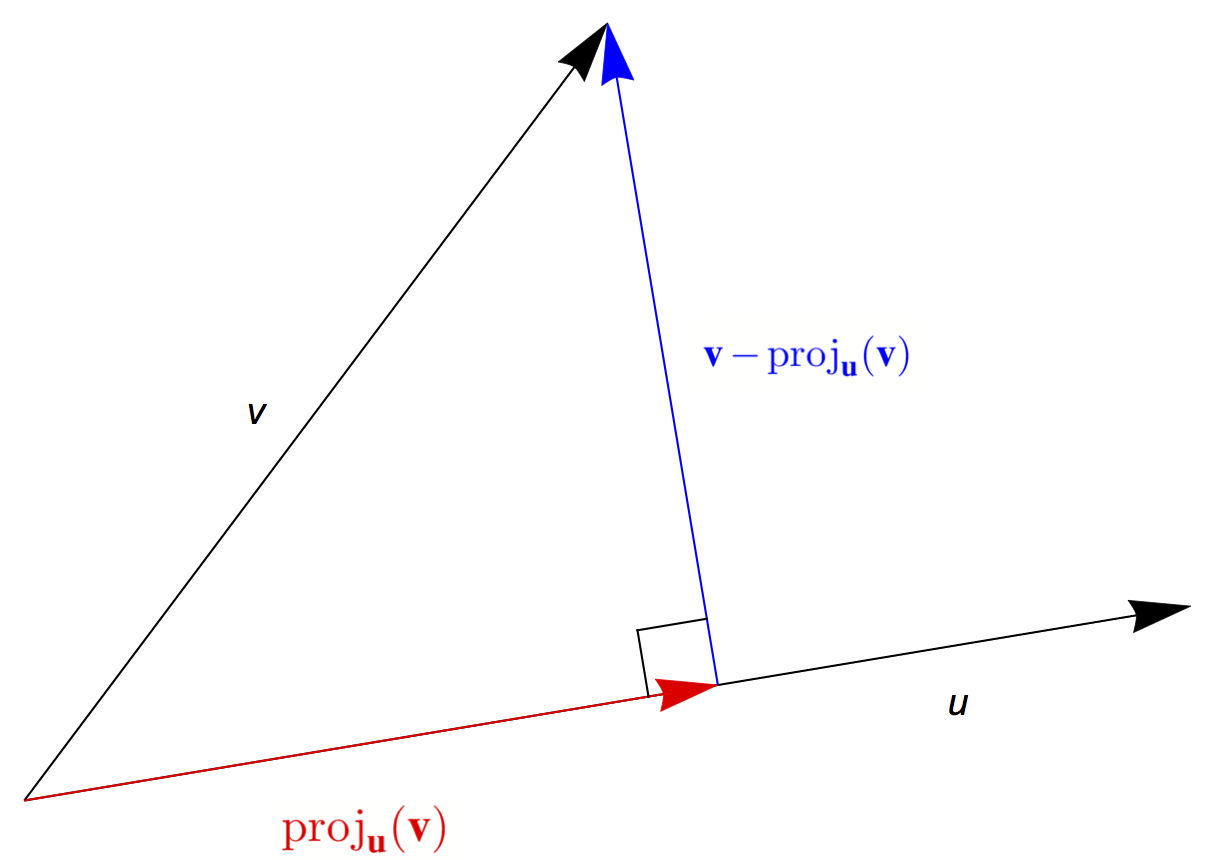
\includegraphics[scale=.4]{decomp.jpg}~\\[1cm]
\end{center}
\caption{Projection orthogonale de $\vv$ sur $\uu$.}\label{orthoprojonvector}
\end{figure}
En particulier, ceci permet de \stress{décomposer} n'importer quel vecteur  $\vv$ comme la somme suivante :
$$
\vv = (\proj_{\uu}(\vv))+ (\vv-\proj_{\uu}(\vv)),
$$
dont le premier terme est un vecteur parallèle à $\uu$ et le second est un vecteur perpendiculaire à $\uu$,
comme représentés dans notre figure \ref{orthoprojonvector}.

Alors comment calcule-t-on $\proj_{\uu}(\vv)$ ?  Ceci s'avère en fait facile.
En utilisant la trigonométrie, ou en résolvant directement les deux conditions ci-dessus, on aboutit à :
$$
\proj_{\uu}(\vv) = \frac{\vv \cdot \uu}{\Vert \uu \Vert^2} \,\uu.
$$\label{projR3}
(Attention : le quotient est juste un scalaire.  Pour s'en souvenir :
si vous projettez $\vv$ sur $\uu$, le résultat est toujours un vecteur qui est un multiple scalaire du vecteur $\uu$. Notez que c'est le même $\uu$ qui apparaît aussi dans la norme au dénominateur).

\begin{myexample}
Soient $\uu = (1,0,0)$ et $\vv = (2,3,4)$.  Écrivons $\vv$ comme une somme
de deux vecteurs, l'un parallèle à $\uu$ et l'autre orthogonal à $\uu$.
(Bien sûr, c'est toujours possible de «~deviner à tâtons~» la réponse, mais voyons plutôt ce que donne la formule).
On calcule
$$
\proj_{\uu}(\vv) = \frac{\vv \cdot \uu}{\Vert \uu \Vert^2} \,\uu
= \frac{2+0+0}{1^2+0^2+0^2}\mat{1\\0\\0} = \mat{2\\0\\0}
$$
et $\vv - \proj_{\uu}(\vv) = (2,3,4)-(2,0,0) = (0,3,4)$. Notre
décomposition est alors
$$
\vv = \mat{2\\3\\4} = \mat{2\\0\\0}+\mat{0\\3\\4}
$$
et il est clair qu'on a obtenu le bon résultat : le premier vecteur est parallèle à $\uu$ tandis que 
le second lui est orthogonal. Notez que c'est la seule
paire de vecteurs à satisfaire ceci.
\end{myexample}

\begin{myexample} 
Soient $\uu = (1,1)$ et $\vv = (2,3)$.  Alors
$$
\proj_{\uu}(\vv) = \frac{\vv \cdot \uu}{\Vert \uu \Vert^2} \uu
= \frac{2+3}{1^2+1^2}\mat{1\\1} = \mat{5/2\\5/2}
$$
est la projection de $(2,3)$ sur $(1,1)$.
\end{myexample}

Dans la vie de tous les jours, la projection orthogonale est utilisée dans le système UMTS (système universel de télécommunications mobiles) pour corriger les perturbations et les erreurs dans les signaux, et pour produire des communications plus fiables.

Remarque : une autre façon d'interpr\'eter la projection orthogonale est de dire que
nous trouvons le point le plus proche de $\vv$ sur la droite passant par l'origine et dirigée par $\uu$.  
Notre prochain objectif est donc de discuter de droites et de plans.



   
\section*{Exercices}
\addcontentsline{toc}{section}{Exercices}

La solution des exercices marqués par un astérisque $\star$ se trouvent à la fin du livre. Essayez-les d'abord avant de consulter la solution.


\begin{prob}
\label{prob02.1}
Donnez l'expression du vecteur nul de $\R^2$, de $\R^3$ et de $\R^5$.
\end{prob}

\begin{prob}
\label{prob02.2}
Montrez que $\uu + (\vv + \ww) = (\uu + \vv) + \ww$ pour tous $\uu,\vv,\ww\in\R^3$.
\end{prob}
 

\begin{prob}
\label{prob02.3}\sov~Soient $A=(1,\ 2,\ 3),\ B=(-5,\ -2,\ 5)$ et $C=(-2,\ 8,\ -10)$,
et soit $D$ le milieu du segment $\overline{AB}$. Trouvez les coordonnées
du milieu du segment $\overline{CD}$.
% $(-2,\ 4,\ -3)$

\end{prob}
\begin{prob}
\label{prob02.4} Résoudre les questions suivantes en utilisant le produit scalaire.\medskip
\begin{enumerate} [a)]
\item Trouvez toutes les valeurs $k\in\R$ telles que les vecteurs $(k,\ k,\ 1)$ et $(k,\ 5,\ 6)$ sont orthogonaux.\medskip % -3 et -2
\item\sov ~Trouvez l'angle entre les vecteurs $ (0,\ 3,\ -3)$ et $ (-2,\ 2,\ -1)$.\medskip % $\pi/4 
\item Si $A=(2,\ 4,\ 1),\ B=(3,\ 0,\ 9)$ et $C=(1,\ 4,\ 0)$, trouver l'angle $ \angle BAC$.  \medskip
% $3\pi/4

\end{enumerate}

\end{prob}

\begin{prob}
\label{prob02.5}\sov~Résoudre les problèmes suivants. \medskip
\begin{enumerate}[a)]

\item Si $\uu=(2,\ 1,\ 3)$ et $\vv=(3,\ 3,\ 3)$, trouvez
 $\proj_{\vv}{\uu}$.  \medskip
%${{2}\over{3}}(3,\ 3,\ 3)$.
\item Si $\uu=(3,\ 3,\ 6)$ et $\vv=(2,\ -1,\ 1)$, trouver
$\|\proj_{\vv}{\uu}\|$. \medskip
%$(3\sqrt6)/2
\item Trouver l'angle entre le plan d'équation cartésienne $x-z=7$ et le plan d'équation $y-z=234$.
\medskip

\end{enumerate}

\end{prob}



 

 
 
\chapter{Droites, plans}
\label{chapter:Fr_03-linesplanes}

Dans le chapitre précédent, nous avons rappelé l'algèbre et la géométrie des vecteurs de
$\R^2$ et de $\R^3$, puis nous avons généralisé à $\R^n$ les notions d'addition vectorielle,
de multiplication scalaire, de produit scalaire, d'orthogonalité et d'angle entre deux vecteurs.  


Dans ce qui suit, nous considérerons les droites de $\R^2$, ainsi que les droites et les plans de $\R^3$.  
Nous verrons que certaines notions se généralisent facilement
à $\R^n$, mais que d'autres demandent plus de travail pour aboutir à une généralisation convenable. En fait, trouver ce qui est exactement
l'analogue d'une droite ou d'un plan dans $\R^n$ est l'un de nos objectifs dans ce cours.


\section{Description des droites}

Dans $\R^2$ ou $\R^3$, une droite est définie de manière unique simplement en se donnant un point par lequel elle passe et
un vecteur qui lui donne une direction. 
\begin{figure}
\begin{center}
\vglue-.7cm

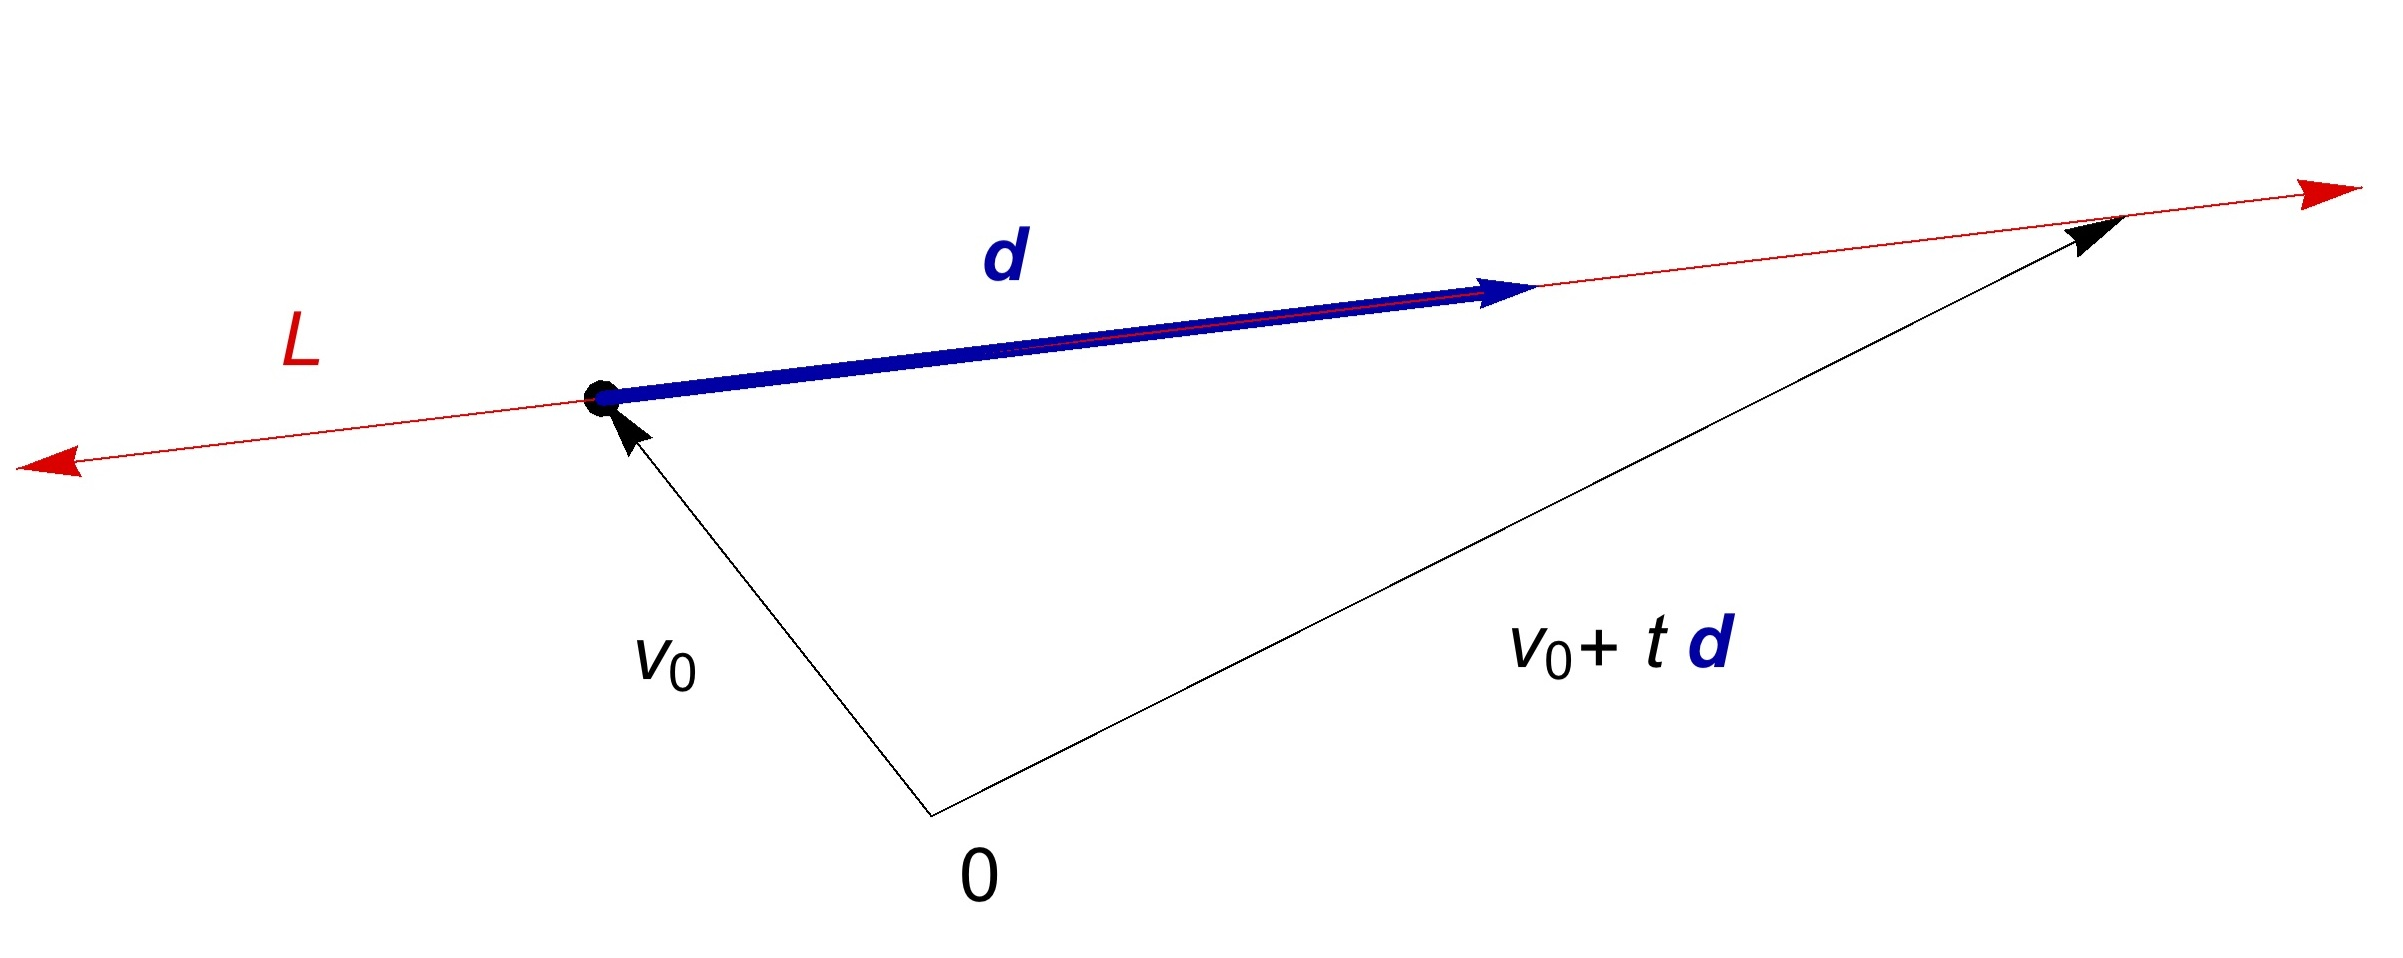
\includegraphics[scale=.1]{linepoint-directionvector.jpg}
\end{center}

\caption{Forme paramétrique vectorielle de $\mathcal L$}\label{vectorparametricformplane}
\end{figure}
Ainsi, la droite $\mathcal L$ passant par le sommet de $\vv_0$ et parallèle à un vecteur $\dd$
est unique et est décrite par l'ensemble
$$
\mathcal L = \{ \vv_0 + t \dd\, |\, t\in \R\}.
$$
En d'autres termes, tout point $\vv$ de la droite $\mathcal L$ peut être écrit comme $\vv = \vv_0+t\dd$ pour un certain $t$. Le vecteur $\dd$ est appelé \defn{vecteur directeur} de $\mathcal L$.

\begin{myexample}
Considérons la droite $y=3x+2$ dans $\R^2$.  Nous pouvons obtenir une équation paramétrique de cette droite en posant $x=t$ comme paramètre et en isolant $y$, et on obtient : 
$x = t$ et $y=3t+2$.  Il est possible de passer à la forme paramétrique vectorielle avec les étapes suivantes :
$$
\mat{x\\y} = \mat{t\\3t+2} = \mat{0+1t\\2+3t} = \mat{0\\2} + t\mat{1\\3}\,.
$$
Ainsi la droite $\mathcal L$ est décrite par
$$
\mathcal L = \left\{ \mat{0\\2} + t\mat{1\\3} \Big| \, t \in \R\right\}.
$$


Remarque : Une autre façon d'obtenir une équation paramétrique de la droite $\mathcal L$ est de prendre deux
points par lesquels elle passe, par exemple $(0,2)$ et $(-\frac{2}{3},0)$, puis de construire le vecteur directeur $\dd$ en calculant la soustraction
$$\dd = \mat{0\\2}-\mat{-2/3\\0} = \mat{2/3\\2}.$$
Maintenant, en prenant par exemple $\vv_0 = (0,2)$, on obtient alors :
$$
\mathcal L = \left\{ \mat{0\\2} + t\mat{2/3\\2} \Big|\, t\in\R\right\}.
$$
Notez qu'on obtient une expression différente de celle qu'on avait précédemment pour $\mathcal L$ : en fait, cette manière d'écrire $\mathcal L$ n'est pas unique car elle dépend de nos choix (on aurait pu plutôt prendre $\vv_0 = (-\frac{2}{3},0)$ par exemple, ou prendre un vecteur $\dd$ deux fois plus grand par exemple). Malgré tout, même si les écritures sont différentes, elle décrivent en fait la même droite $\mathcal L$, et donc plusieurs réponses peuvent être justes (vérifiez ceci avec un dessin !).
\end{myexample}

ATTENTION !  Nous utilisons souvent la variable $t\in\R$ comme paramètre pour une droite, mais si
on veut comparer deux droites différentes, il faut prendre le soin d'utiliser des
lettres différentes, par exemple $t$ et $s$, pour représenter les paramètres dans leurs équations respectives !


\begin{myexample}
Trouvez le point d'intersection (s'il existe) des droites $\mathcal L = \{ t(1,2) \,| \, t \in \R\}$ 
et $\mathcal L' = \{ (0,1)+t(3,0) \,|\, t \in \R\}$.

MAUVAISE M\'ETHODE :  résoudre pour $t$ l'équation vectorielle $t(1,2)=(0,1)+t(3,0)$.
Cette méthode ne donne pas de solution $t$... En fait, ça vient du fait que
les deux droites n'arrivent pas au point d'intersection au même temps $t$. Pourtant, sur un dessin, on voit que ces deux droites se croisent. Elles se croisent donc avec des paramètres $t$ et $s$ différents !


MÉTHODE CORRECTE : Trouver les paramètres $s$ et $t$ tels que
  $t(1,2) = (0,1)+s(3,0)$.  On obtient $t=\frac12$ et $s=\frac16$ et donc le point d'intersection est $(\frac12,1)$. Ouf !
\end{myexample}

Pour une droite de $\R^n$, la forme
$$
\mathcal L = \{ \vv_0 + t \dd~|~ t\in \R\}
$$
 est appelée \defn{forme vectorielle} de $\mathcal L$ ou \defn{forme paramétrique vectorielle} de $\mathcal L$. 
Remarquez que dans $\R^2$, on peut aussi décrire une droite $\mathcal L$ par une équation du type
$ax+by=c$, qu'on appelle \emph{équation cartésienne}\index{equation cartesienne@équation cartésienne} de $\mathcal L$, mais PAS dans $\R^3$ car sinon cette équation décrirait alors un plan !! Voir section \ref{section : description des plans dans R3}.

Notez que la forme paramétrique nous permet aussi d'obtenir des équations paramétriques. Par exemple dans $\R^3$, si l'on se donne $\vv_0 = (a,b,c)$ et $\dd = (d_1,d_2,d_3)$, alors notre droite $\mathcal L$ est l'ensemble de tous les points $\vv=(x_1,x_2,x_3)$ tels que 
\begin{align*}
x_1 &= a+ td_1,\\
x_2 &= b+td_2,\\
x_3 &= c+td_3,
\end{align*}
pour un certain paramètre $t\in \R$.

\section{Remarques sur la géométrie des droites}

Voici quelques observations à propos des droites :
\begin{itemize}
	\item Il n'y a qu'une seule droite dans $\R$: c'est la droite réelle $\R$ elle-même...
	\item Deux droites disjointes dans $\R^2$ peuvent soit être parallèles, soit se croiser en un unique point.
	\item Deux droites disjointes dans $\R^3$ peuvent soit être parallèles, soit se croiser en un unique point, soit être gauches.  Dans les deux premiers cas, elles sont contenues
dans un plan (qui est même unique), mais dans le troisième cas il n'existe pas de plan qui les contient toutes les deux (par contre, on peut trouver deux plans parallèles distincts contenant chacun une des deux droites).
\end{itemize}

\section{Description des plans dans \texorpdfstring{$\R^3$}{R3}}
\label{section : description des plans dans R3}

Rappelez-vous que les plans dans $\R^3$ peuvent être décrits par une équation cartésienne; c'est-à-dire par
l'ensemble des points $(x,y,z)$ tels que
$$
ax+by+cz = d\,,
$$
où $\nn = (a,b,c)$ est un \emph{vecteur normal} au plan,
et où $d\in \R$.

Comment avons-nous obtenu cette équation? 
Si $\vv_0$ est un point quelconque du plan, alors un point $\vv$ appartient au plan ssi $(\vv - \vv_0) \cdot \nn = 0$.  
\begin{figure}
\begin{center}


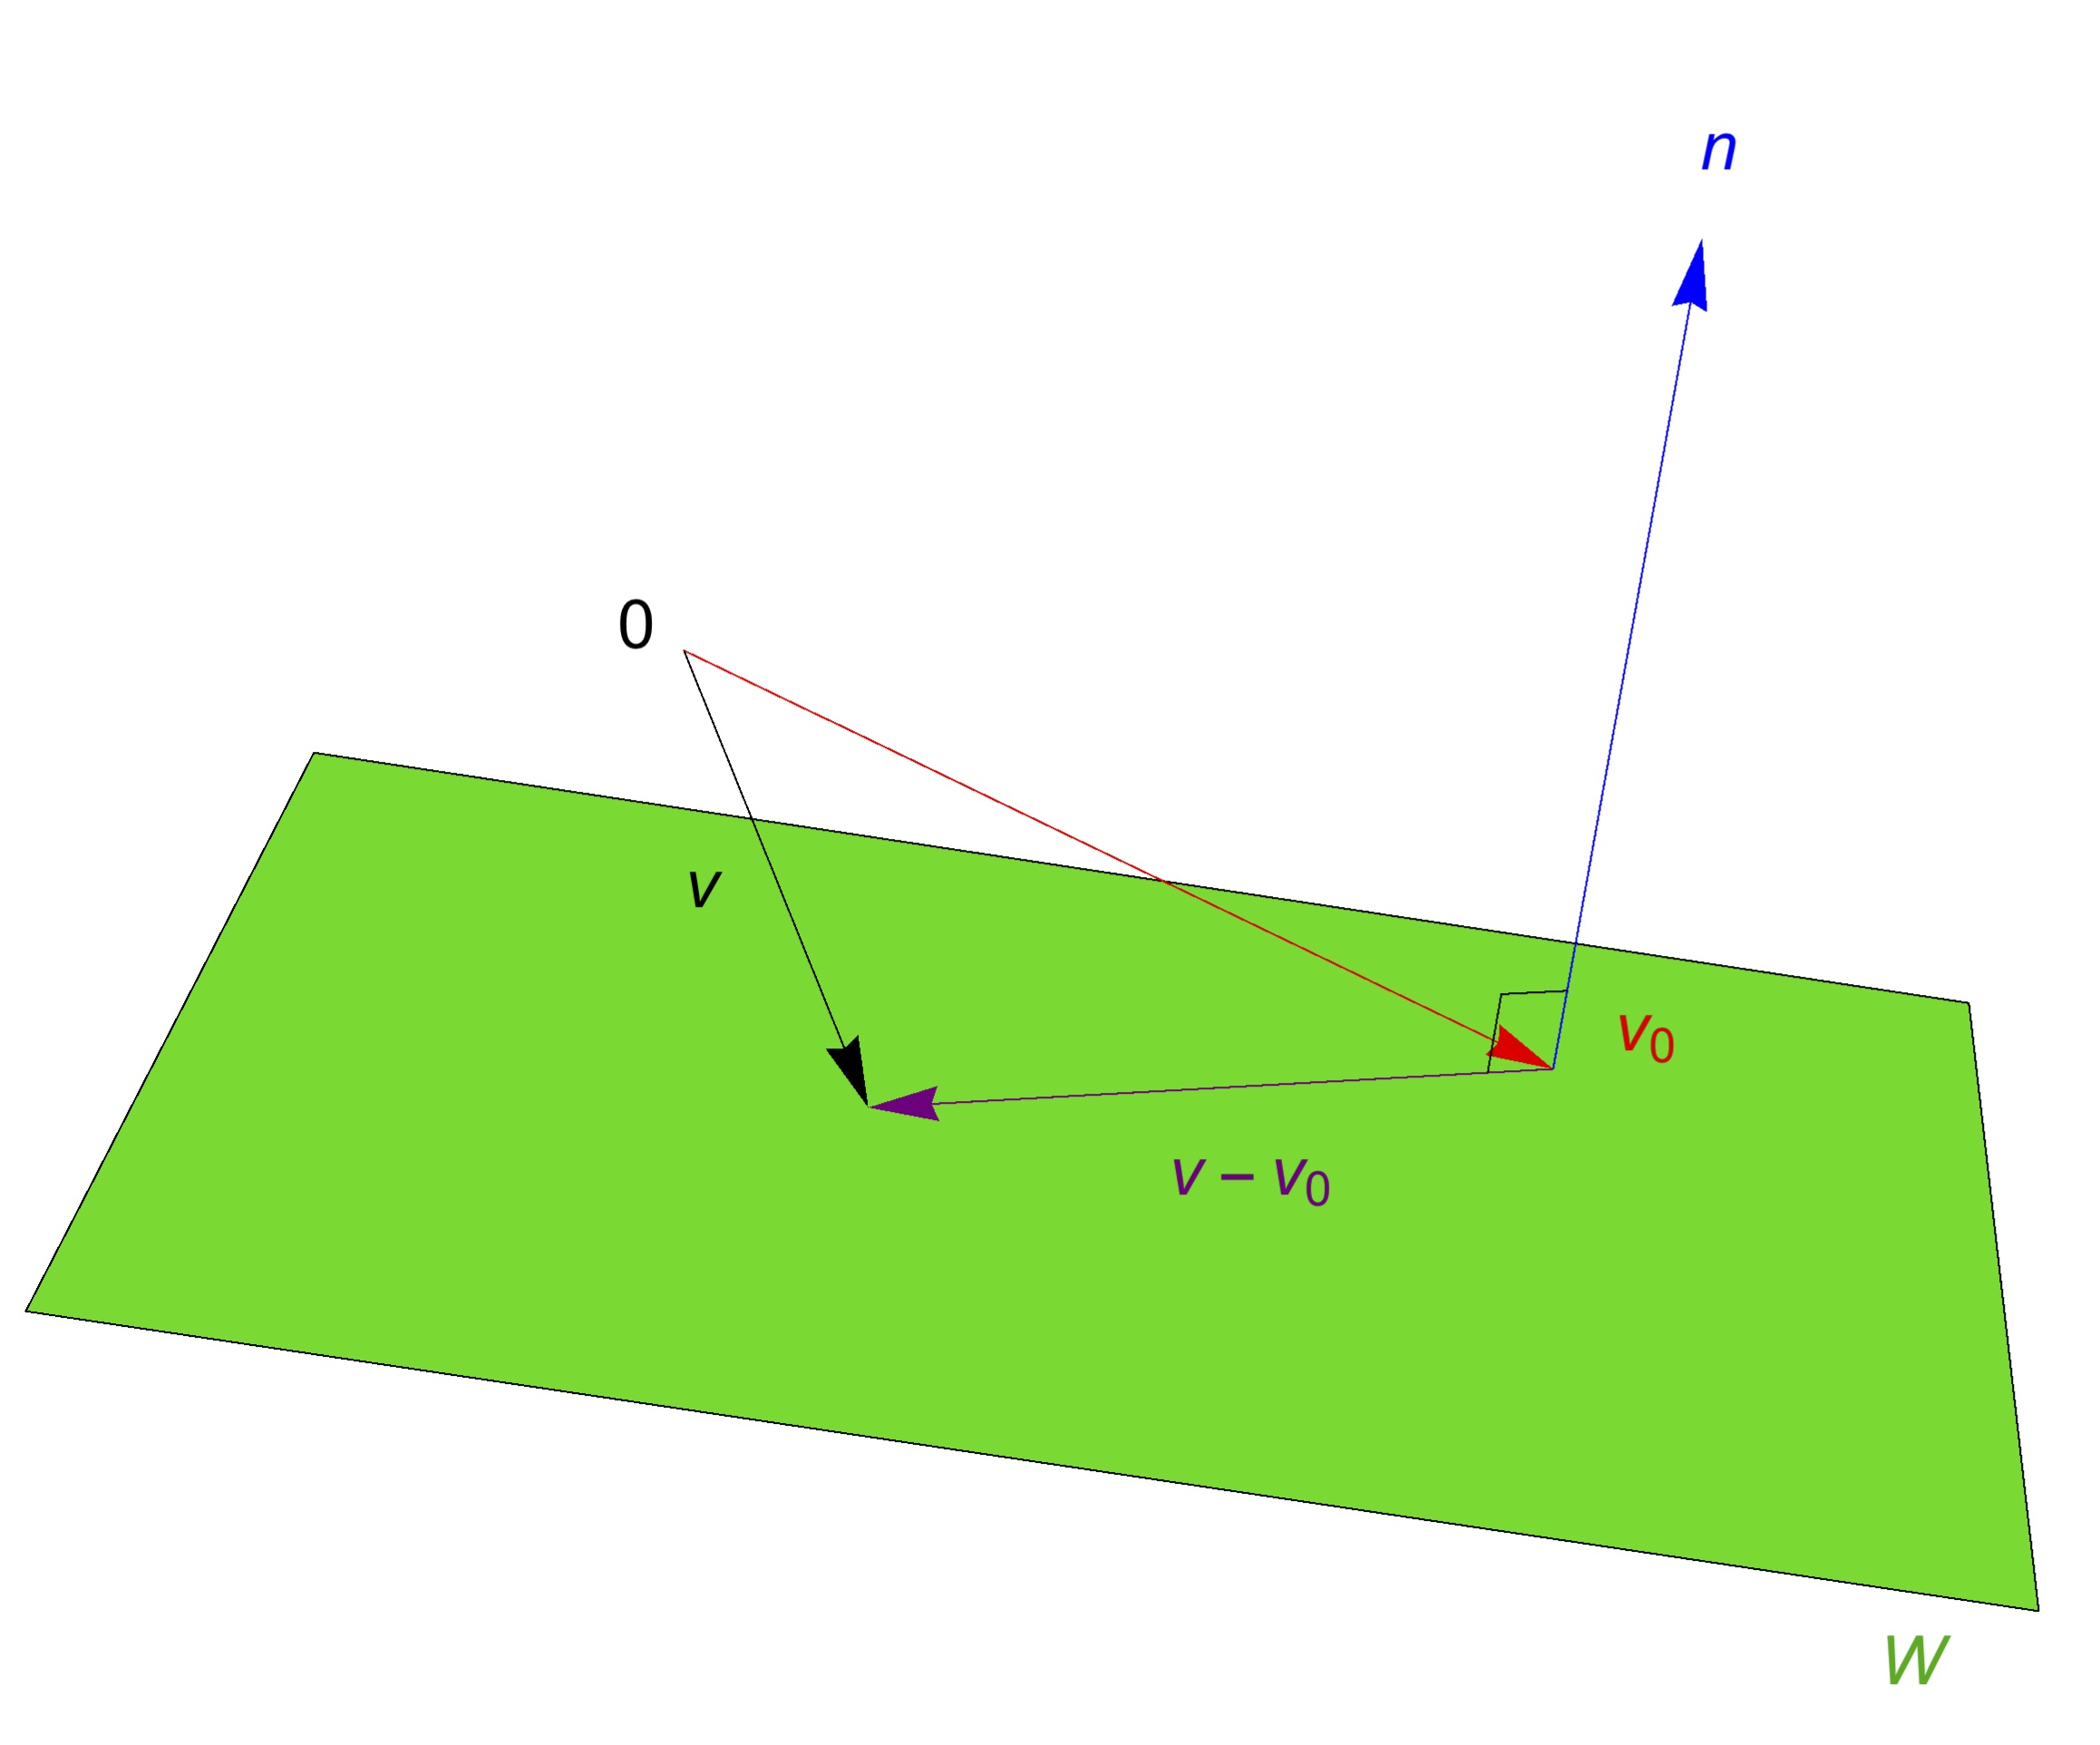
\includegraphics[scale=.087]{cartesianequationplane.jpg}
\end{center}

\caption{\'Equation cartésienne d'un plan}\label{cartesiannormalformalplane}
\end{figure}

Donc le plan passant par $\vv_0$ et de vecteur normal $\nn$ est donné par
$$
\mathcal W = \{ \vv \in \R^3 | (\vv - \vv_0) \cdot \nn = 0 \}.
$$

\begin{myexample}
Le plan passant par $\vv_0 = (1,0,3)$ et de vecteur normal $\nn = (-1,1,2)$
est
\begin{align*}
\mathcal W &= \{ \vv \in \R^3 | (\vv-\vv_0)\cdot \nn=0\}\\
&= \{ (x,y,z) | ((x,y,z)-(1,0,3))\cdot (-1,1,2)=0\}\\
&= \{ (x,y,z) | -(x-1)+(y-0) + 2(z-3) = 0\}\\
&= \{ (x,y,z) | -x+y+2z = 5\}\,.
\end{align*}
(Notez que les coefficients dans l'équation cartésienne nous permettent de retrouver l'expression d'un vecteur normal).
\end{myexample}

Le vecteur normal est utile dans de nombreuses situations. En voici un exemple.

\begin{myprob} 
Trouvez la distance du point $P = (1,2,3)$ au plan $\mathcal W$ d'équation cartésienne $3x-4z=-1$.

\begin{mysol} 


Soit $A$ un point quelconque du plan $\mathcal W$, disons $A=(1,0,1)$, et soit $Q$ le point (inconnu) du plan $\mathcal W$ le plus proche de $P$. En d'autres termes $Q$ est la projection orthogonale\footnote{Voici une preuve. Si $Q'$ est un autre point quelconque sur $\mathcal W$, $\|P-Q'\|^2=\|P-Q+ Q-Q'\|^2= \|P-Q\|^2+ \|Q-Q'\|^2$ (car $P-Q$ et $Q-Q'$ sont perpendiculaires, donc le théorème de Pythagore s'applique). Ainsi $\|P-Q'\|^2\ge \|P-Q\|^2$. } de $P$ sur $\mathcal W$, voir la définition dans la section \ref{section : projection orthogonale sur une droite dans Rn}.
Comme on peut le voir sur la figure ci-dessous, ceci revient à calculer la longueur de la projection du vecteur rouge $\mathbf{PA}=A-P$ sur le vecteur normal $\nn$ en bleu.


\begin{center}

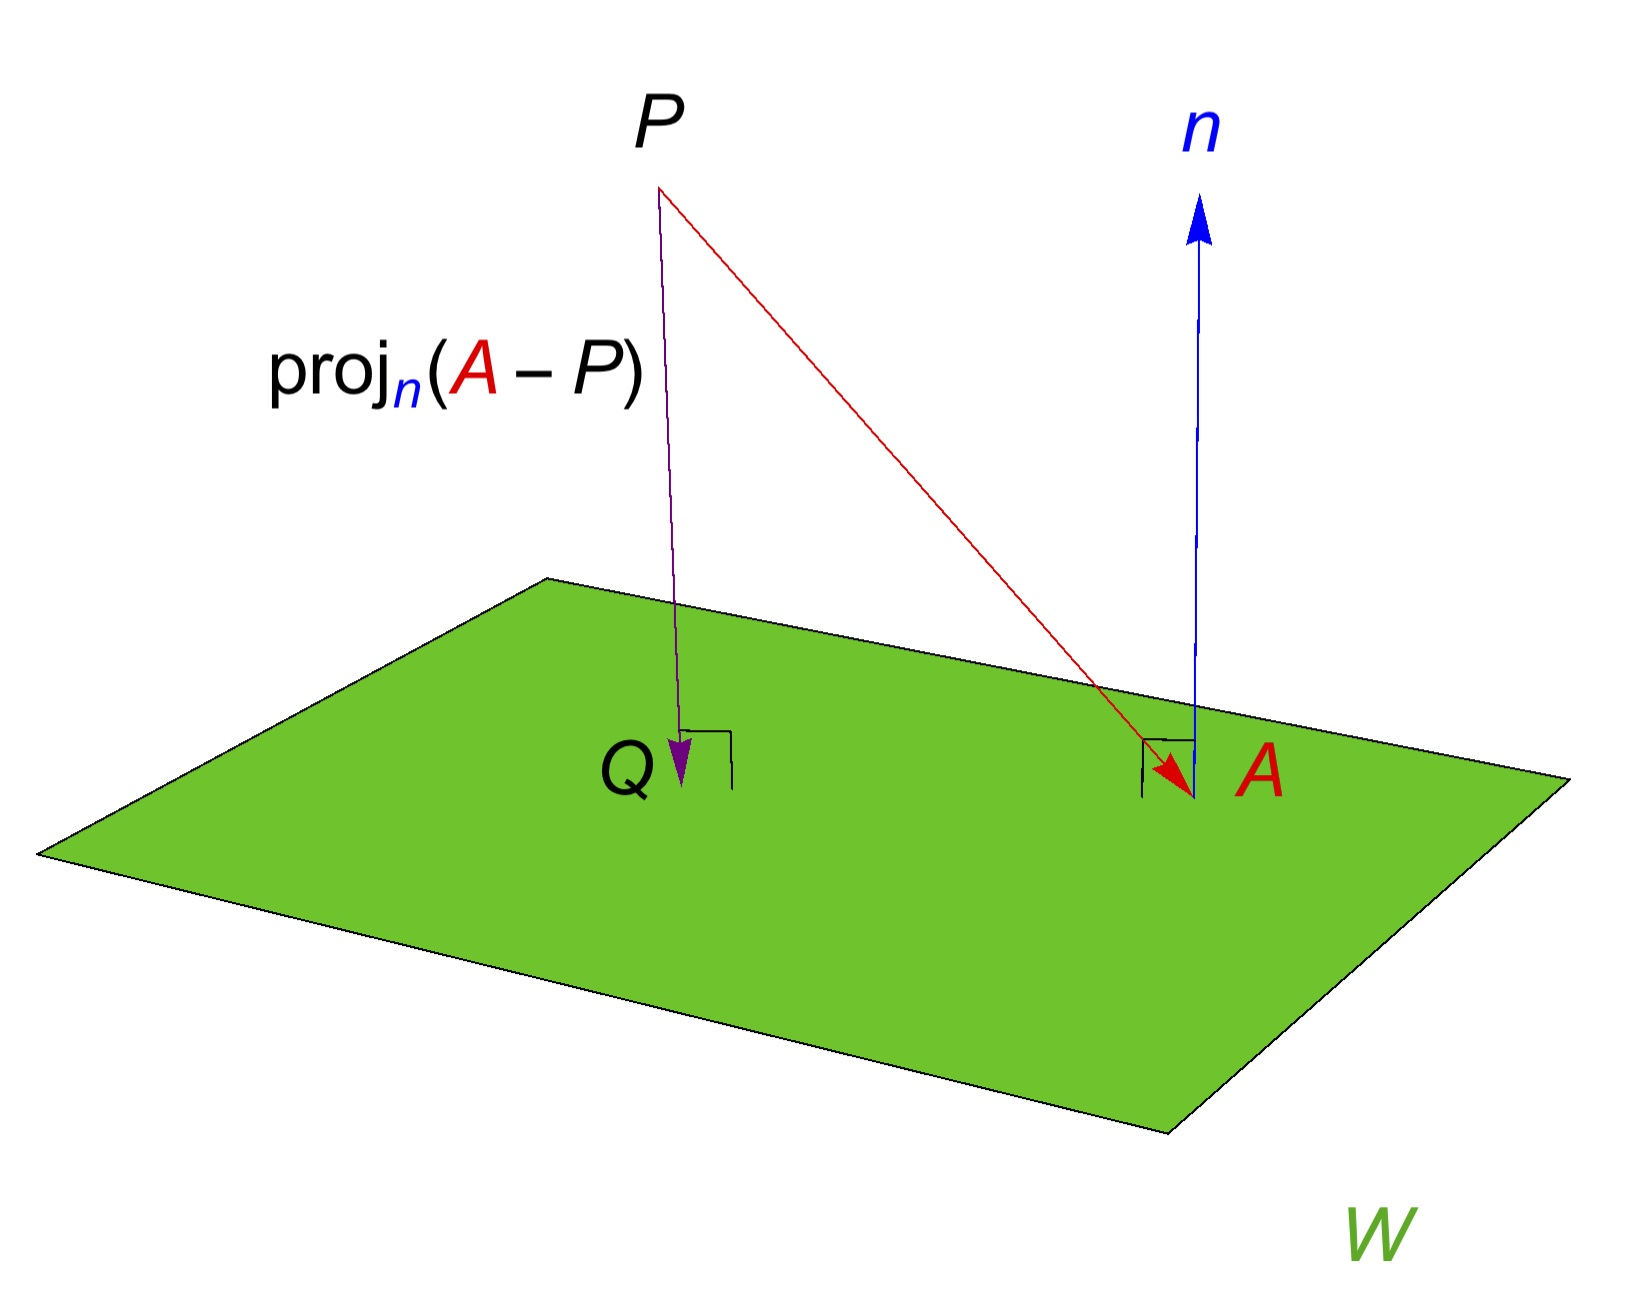
\includegraphics[scale=.4] {projP_on_W.jpg}\\
Distance du point $P$ au plan $\mathcal W$.

\end{center}

On a donc
\begin{align*}
\Vert P-Q \Vert &= \Vert {\proj}_{\nn}(P-A) \Vert\\
&= \Vert {\proj}_{(3,0,-4)}(0,2,2) \Vert\\
&= \Big\Vert \frac{0+0-8}{3^2+(-4)^2}(3,0,-4) \Big\Vert\\
&= \frac{8}{25} \Vert (3,0,-4) \Vert\\
&= \frac{8}{25} \sqrt{25} = \frac{8}{5}.
\end{align*}
\end{mysol}
\end{myprob}

Dans ce qui suit, nous abordons une question plus simple : l'intersection de
deux plans.


\begin{myprob} Trouvez l'intersection des plans $x+y+z = 3$ et $x-y-z=2$.

\begin{mysol} Nous devons trouver tous les points $(x,y,z)$ qui satisfont les deux équations.
Si on soustrait la deuxième équation de la première, on obtient $2y+2z = 1$, ce qui donne $y = \frac12-z$. Alors, à partir de la première équation, nous avons $x = 3-(\frac12-z)-z
= \frac52$.  Mais $z$ peut être arbitraire et donc on peut le considérer comme paramètre (appelons le $t$). On a alors
$$
x = \frac52, \quad y=\frac12-t, \quad z=t
$$
qui est la droite suivante (écrite sous forme vectorielle) :
$$
\mathcal L= \left\{ \mat{5/2\\1/2\\0} + t \mat{0\\-1\\1} | t\in \R\right\}.
$$
\end{mysol}\end{myprob}

\section{Géométrie des plans dans \texorpdfstring{$\R^3$}{R3}}

On définit l'« angle » entre deux plans comme étant l'angle aigu entre deux de leurs vecteurs normaux  
(bien que prouver que ceci à un sens demande quelques réflexions).

Avant de développer plus, comparons les plans de $\R^2$ avec ceux de $\R^3$ :
 
\begin{itemize}
	\item Le seul plan dans $\R^2$ est... $\R^2$ lui-même !

	\item $\R^3$ admet une infinité de plans, et deux plans disjoints de $\R^3$ peuvent soit être parallèles, soit se couper en une droite.
\end{itemize}

Après ceci, on peut alors se poser des questions sur $\R^4$, n'est-ce pas ?
Ceci dit, nous n'avons pas de bonne façon pour décrire (pour l'instant) un plan dans ${\R^4}$, ni même dans $\R^n$ de manière générale pour tout $n\geq 4$ :
en effet, une équation paramétrique vectorielle en une variable donne une droite; et une équation cartésienne donne un hyperplan de dimension $n-1$...  En fait, les équations cartésiennes donnent des objects différents selon la dimension de $\R^n$:

\begin{center}
\begin{tabular}{cccc}
$n$ & & \'Equation dans $\R^n$& Objet géométrique \\ 
\hline
1 &\hphantom{XX} & $ax=b$ & point \\
2 & & $ax+by=c$ & droite \\
3 & & $ax+by+cz =d$ & plan\\
4 & & $ax_1+bx_2+cx_3+dx_4=e$ & ??
\end{tabular}
\end{center}

L'idée derrière tout ça est qu'une équation réduit le \stress{degré de liberté}
(ou la \defn{dimension}, pour utiliser la terminologie \`a venir), et donc le résultat est toujours un objet
de \stress{dimension $n-1$} appelé un \defn{hyperplan} lorsque $n-1\geq3$.

Voici ce qu'on se dit:  puisque l'intersection non-vide de deux plans disjoints de ${\R^3}$ est une droite, l'intersection non-vide de deux hyperplans disjoints de $\R^4$ devrait donner un plan. Wow !
C'est une idée sur laquelle nous reviendrons dans les prochains chapitres.

Mais pour l'instant, revenons à quelque chose de plus concret, dans $\R^3$,
et regardons comment construire facilement des vecteurs normaux d'un plan.

\section{Produit vectoriel dans \texorpdfstring{$\R^3$}{R3}}

Tout d'abord, on adopte la notation suivante :
$$
\hat{i} = \mat{1\\0\\0}, \quad \hat{j} = \mat{0\\1\\0}, \quad \hat{k} = \mat{0\\0\\1}.
$$
Cette notation est intéressante puisqu'alors $(x,y,z) = x\,\hat{i} + y\,\hat{j} + z\,\hat{k}$.

Dans la suite, nous utiliserons également la notation du \emph{d\'eterminant} qui est très pratique à ce niveau.
Le \defn{produit vectoriel} de $\uu = (x,y,z)$ et $\vv=(x', y', z')$
est le vecteur noté $\uu \times \vv$ et donné par 

\begin{align*}
\uu \times \vv &= \left| \begin{matrix}
\hat{i} & \hat{j} & \hat{k} \\
x & y & z\\
x' & y' & z' \end{matrix} \right|\\
&= \left( yz' - y'z, -(xz' - x'z), xy' - x'y \right) \\
&= \left( \left| \begin{matrix} y & z\\ y' & z' \end{matrix} \right|,
- \left| \begin{matrix} x & z\\ x' & z' \end{matrix} \right|,
\left| \begin{matrix} x & y\\ x' & y' \end{matrix} \right| \right)\,.
\end{align*}

\begin{myprob}
Calculez $(1,2,3)\times(4,5,6)$.

\begin{mysol}  Écrivez ceci comme un déterminant puis développez :
$$
\left| \begin{matrix}
\hat{i} & \hat{j} & \hat{k} \\
1 & 2 & 3\\
4 & 5 & 6 \end{matrix} \right|
= (12-15, -(6-12), 5-8) = (-3,6,-3). 
$$
\end{mysol}\end{myprob}

\begin{myprob} Déterminez $(4,5,6)\times(1,2,3)$.

\begin{mysol} De même que dans l'exercice précédent on a :
$$
\left| \begin{matrix}
\hat{i} & \hat{j} & \hat{k} \\
4 & 5 & 6\\
1 & 2 & 3 \end{matrix} \right|
= (15-12, -(12-6), 8-5) = (3,-6,3)\,,
$$
Notez qu'on a obtenu le vecteur opposé à celui d'avant :  $(4,5,6)\times(1,2,3) = -\,(1,2,3)\times(4,5,6)$. 
\end{mysol}\end{myprob}

Par ailleurs, on remarque que :
$$
(1,2,3)\cdot (3,-6,3) = 3-12+9 = 0, \quad (4,5,6)\cdot (3,-6,3) = 12-30+18=0.
$$
Mais rien de tout cela n'est le fruit du hasard!

\begin{theorem} [Propriétés du produit vectoriel]   \label{theoreme : proprietes du produit vectoriel}
Soient $\uu,\vv,\ww\in \R^3$.  Alors :
\begin{itemize}
\item $\uu \times \vv = -\,\vv \times \uu$;
\item $(\uu \times \vv)\cdot \uu = 0$;
\item $(\uu \times \vv)\cdot \vv = 0$;
\item $(\uu + \vv)\times \ww = \uu \times \ww + \vv \times \ww$;
\item $\Vert \uu \times \vv \Vert = \Vert \uu \Vert \; \Vert \vv \Vert \sin(\theta)$, où $0 \leq \theta \leq \pi$ est l'angle entre $\uu$ et $\vv$.
Il s'agit en fait de l'aire du parallélogramme formé par $\uu$ et $\vv$.
\end{itemize}
Notez qu'en général $\uu \times (\vv \times \ww) \neq (\uu \times \vv) \times \ww$; par exemple : $\hat{i} \times (\hat{k} \times \hat{k}) = \zero$ mais $(\hat{i} \times \hat{k})\times \hat{k} = -\hat{i}$. Par conséquent, 
le produit vectoriel n'est ni commutatif ni associatif. 
\end{theorem}


Ainsi, si deux vecteurs $\uu$ et $\vv$ sont parallèles, alors leur produit vectoriel
est nul.  Sinon, leur produit vectoriel est non-nul, c'est l'un des deux vecteurs orthogonaux à la fois à 
$\uu$ et à $\vv$, de longueur $\Vert \uu \Vert \; \Vert \vv \Vert \sin\theta$, où $\theta$ est l'angle entre $\uu$ et $\vv$.
Le produit vectoriel est utilisé par exemple en physique pour mesurer le moment d'une force (le moment traduit l'aptitude de cette force à faire tourner un système mécanique autour d'un point). Il sert aussi à déterminer le troisième vecteur d'une base de $\R^3$ avec la règle des trois premiers doigts de la main droite. Notez qu'une formule facile à retenir est $\hat{i} \times \hat{j} = \hat{k}$ et ses permutations cycliques.

\section[Application: les vecteurs normaux]{Première application du produit vectoriel : Les vecteurs normaux}

Le produit vectoriel donne un vecteur normal aux plans définis par $\uu$ et $\vv$.

\begin{myprob}
Trouvez l'équation du plan contenant les trois points $A = (1,2,3)$,
$B = (1,0,0)$ et $C = (0,1,1)$.

\begin{mysol}
Les vecteurs $\mathbf{BA} = (0,2,3)$ et $\mathbf{BC} = (-1,1,1)$ sont tous les deux
parallèles au plan passant par $A,B,C$, donc tout vecteur $\nn$ normal au plan doit être orthogonal à chacun des deux vecteurs, et la réciproque est aussi vraie. Par le théorème \ref{theoreme : proprietes du produit vectoriel}, on peut donc prendre le produit vectoriel des deux vecteurs :
$$
\nn
=
\mathbf{BA} \times \mathbf{BC}
=
 \left| \begin{matrix}
\hat{i} & \hat{j} & \hat{k} \\
0 & 2 & 3\\
-1 & 1 & 1 \end{matrix} \right| = (-1, -3, 2)\,.
$$
(Vérifiez votre réponse!  Ce vecteur $\nn$ devrait être orthogonal à $\mathbf{BA}$ et à $\mathbf{BC}$.)

L'équation du plan a donc la forme suivante :
$$
-x -3y + 2z = d\,.
$$
Enfin, pour trouver $d$, on utilise un point du plan, disons $B= (1,0,0)$, et on obtient $d=-1$.
\end{mysol} \end{myprob}

\section[Application: volume d'un parallélépipède]{Deuxième application du produit vectoriel : volumes d'un parallélépipède (produit mixte)}

\begin{theorem} [Volume d'un parallélépipède]
Le volume du parallélépipède dont les côtés sont les vecteurs $\uu$, $\vv$ et $\ww$
de $\R^3$ est
$$
\vert (\uu \times \vv) \cdot \ww \vert. 
$$
Notez que l'ordre des vecteurs n'a pas d'importance.
\end{theorem}

Nous pouvons le prouver en utilisant davantage de trigonométrie. Le volume
du parallélépipède est l'aire de la base (un parallélogramme)
fois sa hauteur. Cependant, l'aire de la base est la norme du produit vectoriel
de deux des vecteurs ($\Vert \uu \times \vv \Vert$) et sa hauteur sera de 
$\Vert \ww \Vert \cos(\theta)$, où $\theta$ est l'angle entre
$\ww$ et un vecteur normal à la base.

\begin{myprob}
Trouvez le volume du parallélépipède dont les côtés sont $\uu = (1,0,1)$,
$\vv = (1,2,2)$ et $\ww = (10,0,0)$.

\begin{mysol}
On a
$$
\uu \times \vv =  \left| \begin{matrix}
\hat{i} & \hat{j} & \hat{k} \\
1 & 0 & 1\\
1 & 2 & 2 \end{matrix} \right| 
= (-2,-1,2)
$$
et donc
$$
(\uu \times \vv)\cdot \ww = (-2,-1,2)\cdot (10,0,0) = -20\,.
$$
D'o\`u le volume est de $20$.
\end{mysol}\end{myprob}

Et quelle déduction peut-on faire si l'on a l'égalité $(\uu \times \vv)\cdot \ww = 0$ ?  
On aurait donc un parallélépipède de volume nul, ce qui signifie que ce n'est pas vraiment un parallélépipède...
En fait, cette égalité signifie que les trois vecteurs se trouvent tous dans le même plan. Nous
dirons que ces vecteurs sont \defn{coplanaires}, puisque contenus dans le même plan, et \emph{linéairement dépendants} (terminologie clé pour la suite), puisqu'on peut exprimer un vecteur en fonction des autres.





\section[Remarques finales: les droites, les plans, et plus encore]{Remarques finales sur les droites, les plans et les objets de dimensions supérieures dans \texorpdfstring{$\R^n$}{Rn}}

Faisons quelques réflexions sur certaines idées
que nous explorerons aux prochains chapitres.  Nous avons introduit
des bons moyens d'exprimer les droites et les plans dans $\R^2$ et $\R^3$ : équations paramétriques et équations cartésiennes. Cependant, dans $\R^4$, ces deux techniques échouent pour décrire un objet «~bi-dimensionnel~» alors que notre intuition nous amène à penser qu'ils existent bel et bien.

Ou bien, peut-être pouvons-nous généraliser les procédés des petites dimensions aux grandes dimensions ?\!?

Pour rappel, pour obtenir une droite, nous avons vu qu'il suffit d'avoir un seul paramètre (un degré de liberté): 
$$
\mathcal L = \{ \vv_0+ t\dd_1 \,|\, t\in\R\}\,.
$$
Si maintenant on utilise deux paramètres $s$ et $t$ et deux vecteurs non colinéaires $\dd_1$ et $\dd_2$, on obtient un plan :
$$
\mathcal W = \{ \vv_0 + s\dd_1 + t\dd_2 \,|\, s,t\in\R\}\,.
$$
En d'autres termes, c'est le plan de vecteur normal $\dd_1 \times \dd_2$ et passant par le point $\vv_0$. Ce sera la clé pour généraliser les notions aux dimensions supérieures.

Nous généraliserons prochainement ce type d'énoncé en vue de mieux comprendre les sous-espaces des espaces vectoriels dans le cas général.





\section*{Exercices}
\addcontentsline{toc}{section}{Exercices}


    
 
\begin{prob}\label{prob03.1}  Répondez aux questions suivantes en n'utilisant que le produit vectoriel et/ou le produit scalaire.
\begin{enumerate}[a)]
\item Pour $\uu=(3,\ -1,\ 4)$ et $\vv=(-1,\ 6,\ -5)$, calculez
$\uu\times \vv$. \medskip
% $(-19,\ 11,\ 17)$
\item\sov~Trouvez tous les vecteurs de $\R^3$ qui sont orthogonaux à la fois à $(-1, 1, 5)$ et à $(2, 1, 2)$.  \medskip
% $\{(t,\ -4t,\ t)|\ t\ dans \R\}$.
\item Si  $\uu=(4,\ -1,\ 7),\ \vv=(2,\ 1,\ 2)$ et 
$\ww=(-1,\ -2,\ 3)$, déterminez $(\uu\times \vv)\times \ww$. \medskip
% $(30,\ 21,\ 24)$
\item\sov~Si $\uu=(-4,\ 2,\ 7),\ \vv=(2,\ 1,\ 2)$ et 
$\ww=(1,\ 2,\ 3)$, déterminez $\uu\cdot (\vv\times \ww)$. \medskip
% 17
\end{enumerate}

\end{prob}
\begin{prob}
\label{prob03.2}  Même consigne qu'à l'exercice précédent. \medskip
\begin{enumerate}[a)]

\item Trouvez l'aire du parallélogramme défini par les vecteurs
$\uu=(1,\ -1,\ 0)$ et $\vv=(2,\ -3,\ 1)$.    \medskip
\item\sov~Trouvez l'aire du triangle dont les trois sommets sont $ A=(-1,\ 5,\ 0) $, $B=(1,\ 0,\ 4)$ et $C=(1,\ 4,\ 0)$.  \medskip
%6
\item Trouvez l'aire du triangle dont les trois sommets sont $P=(1,\ 1,\ -1),\ Q=(2,\ 0,\ 1)$ et\\ $R=(1,\ -1,\ 3)$.  \medskip
%\sqrt{5}


\item\sov~Trouvez le volume du parallélépipède formé par les vecteurs $\uu=(1,\ 1,\ 0),\ \vv=(1,\ 0,\ -1)$\\ et $\ww=(1,\ 1,\ 1)$.\medskip
% 1

\item Trouvez le volume du parallélépipède formé par $\uu=(1, -2, 3),\ \vv=(1,3,1)$ et $\ww=(2,1,2)$.\medskip
% 10

\end{enumerate}



\end{prob} \begin{prob} \label{prob03.3}  Résolvez les problèmes suivants dans $\R^3$. \medskip
\begin{enumerate}[a)]
\item\sov~Trouvez le point d'intersection du plan dont l'équation cartésienne est $2x+2y-z=5$ 
et de la droite d'équations paramétriques $x=4-t,\ y=13-6t,\ z=-7+4t$.\medskip %$(2,\ 1,\ 1)$
\item\sov~Si $\mathcal L$ est la droite passant par $(1,\ 1,\ 0)$ et $(2,\ 3,\ 1)$, trouvez le point d'intersection de $\mathcal L$ avec le plan d'équation cartésienne $x+y-z=1$.\medskip % $(0,\ 1/2,\ -1/2)$
\item Trouvez le point d'intersection de la droite d'équations paramétriques $x=t-1$, $y=6-t,\\ z=-4+3t$ avec la droite d'équations $x=-3- 4t,\ y=6-2t,\ z=-5+3t$. \medskip%(1,\ 4,\ 2)
\item Déterminez si les plans d'équations cartésiennes $2x-3y+4z=6$ et $4x-6y+8z=11$ se croisent ou non. \medskip% Non
\item Trouvez la droite à l'intersection des plans d'équation cartésienne $5x+7y-4z=8$ et\\ $x-y=-8$. \medskip%$(-4,\ 4,\ 0)+ t (1,\ 1,\ 3),\, t\in \R$
\item\sov~Trouvez la droite à l'intersection des plans d'équations cartésiennes $x+11y-4z=40$ et $x -y=-8$. \medskip
%$(-4,\ 4,\ 0)+ t (1,\ 1,\ 3),\, t\in \R$

\end{enumerate}



\end{prob} \begin{prob} \label{prob03.4}  Résolvez les problèmes suivants dans $\R^3$. \medskip
\begin{enumerate}[a)]

\item Trouvez la distance du point $(0,\ -5,\ 2)$ au plan d'équation cartésienne
$2x+3y+5z=2$. \medskip
%7$/\sqrt{38}$.

\item\sov~Trouvez la distance du point $(-2,\ 5,\ 9)$ au plan d'équation cartésienne
$6x+2y-3z=-8$. \medskip
%3
\item Trouvez la distance entre le point $(5,\ 4,\ 7)$ et la droite passant par les points  $(3,\ -1,\ 2)$ et $(3,\ 1,\ 1)$.
\medskip



\item\sov~Trouvez la distance entre le point $(8,\ 6,\ 11)$ et la droite passant par les points $(0,\ 1,\ 3)$ et $(3,\ 5,\ 4)$.  \medskip
% 7
 
\item Trouvez l'angle entre les plans d'équations cartésiennes $x-z=7$ et $y-z=234$.
\medskip
%$\pi/3




\end{enumerate}

\end{prob} \begin{prob} \label{prob03.5}  Trouvez les équations paramétriques {\it et} la forme vectorielle de chacune des droites suivantes :
\medskip
\begin{enumerate}[a)]

\item La droite passant par les points $(3,\ -1,\ 4)$ et $(-1,\ 5,\ 1)$. \medskip
\item\sov~La droite passant par $(-5,\ 0,\ 1)$ et parallèle aux deux plans d'équations cartésiennes\\ $2x-4y+z=0$ et $x-3y-2z=1$. 
\medskip
%$x=-5+11t,\, y=5t,\, z=1-2t,\, t\in \R$
\item La droite passant par $(1,\ 1,\ -1)$ et perpendiculaire au plan d'équations cartésiennes\\ $2x-y+3z=4$. \medskip
%$x=1+2t,\, y=1-t,\, z=-1+3t,\, t\in \R$
\end{enumerate}

\end{prob} \begin{prob} \label{prob03.6}  Trouvez une équation cartésienne pour chacun des plans suivants :

\medskip
\begin{enumerate}[a)]
\item Le plan contenant $(3, -1, 4)$, $(-1, 5, 1)$ et $(0, 2, -2)$.\medskip% $2y - z = 3
\item\sov~Le plan parallèle au vecteur $(1, 1, -2)$ et contenant les points $(1, 5, 18)$ et $(4, 2, -6)$.\medskip %5x - 3y + z = 8
\item Le plan passant par les points $(2, 1, -1)$ et $(3, 2, 1)$ et parallèle à l'axe $x$. \medskip
\item\sov~Le plan contenant les deux droites 
$\set{(t-1,6-t,-4+3t)\st t \in \R}$ et $ \set{(-3 -4t, 6+ 2t, 7+5t)\st t\in \R}$.\medskip  %11x + 17y + 2z = 83
\item Le plan contenant à la fois le point $(-1, 0, 2)$ et la droite à l'intersection des deux plans $3x + 2y - z = 5$ et $2x + y + 2z = 1$.  \medskip %$23x + 12y + 19z = 15$.
\item\sov~Le plan contenant le point $(1, -1, 2)$ et la droite $\set{(4, -1 + 2t,2 + t)\st t \in \R}$. \medskip% $y - 2z + 5 = 0$.
\item Le plan passant par l'origine et parallèle aux deux vecteurs $(1, 1, -1)$ et $(2, 3, 5)$. \medskip%8x - 7y + z = 0$.
\item\sov~Le plan passant par le point $(1,\ -7,\ 8)$ et perpendiculaire à la droite\\ $\set{(2+2t,7-4t,-3+t) \st t\in \R}.$ \smallskip  
%$2x-4y+z=38$
\item Le plan passant par le point $(2,\ 4,\ 3)$ et perpendiculaire aux plans d'équations cartésiennes $x+2y-z=1$ et $3x-4y=2$.  
%$4x+3y+10z=50$.


\end{enumerate}
 

\end{prob} \begin{prob} \label{prob03.7}   Trouvez la forme vectorielle pour les plans $\mathcal W$ dont les équations cartésiennes sont les suivantes 
(c'est-à-dire, trouvez un point $a \in \mathcal W$ et deux vecteurs $\uu, v \in \R^3$ non-nuls et non-parallèles entre eux mais parallèles au plan $\mathcal W$, tels que $\mathcal W=\set{a+ s u + t v\st s,t \in \R}$) :\medskip
\begin{enumerate}[a)]

\item $x - y - z = 3$.\medskip 
\item\sov~$x - y - 2z = 4$. \medskip
\item $2x - y + z = 5$. \medskip
\item $y + 2x = -3$. \medskip
\item $x - y + 2z = 0$. \medskip
\item $x + y + z = -1$.\medskip
\end{enumerate}


\end{prob} \begin{prob} \label{prob03.8}\sov~Soient $\uu, v$ et $\ww$ des vecteurs quelconques de $\R^3$.  Déterminez lesquels des énoncés suivants pourrait être faux et donnez un exemple pour justifier chacune de vos réponses.
 \medskip

(1) $\uu\cdot \vv=\vv\cdot \uu$.

(2) $\uu\times \vv=\vv\times \uu$.

(3) $\uu\cdot(\vv+\ww)=\vv\cdot \uu+\ww\cdot \uu$.

(4) $(\uu+2\vv)\times \vv=\uu\times \vv$.

(5) $(\uu\times \vv)\times \ww=\uu\times(\vv\times \ww)$.

% 2 \& 5

\end{prob} \begin{prob} \label{prob03.9}\sov~Soient $\uu , \vv $ et $\ww $ des vecteurs de $\R^3$.  Lesquels des énoncés suivants sont (toujours) vrais ? Justifiez vos réponses quand c'est VRAI et donnez un contre-exemple lorsque c'est FAUX.
\medskip

(i) $(\uu\times \vv)\cdot \vv=0$.
 

(ii) $(\vv \times \uu)\cdot \vv=-1$.
 

(iii) $(\uu\times \vv)\cdot \ww$ est le volume du parallélépipède formé par $\uu$, $\vv$ et $\ww$.
 

(iv) $||\uu\times \vv||=||\uu||\,||\vv||\,\cos\theta$,
où $\theta$ est l'angle entre $\uu$ et $\vv$.
 

(v) $|\uu\cdot \vv|=||\uu||\,||\vv||\,\cos\theta$,
où $\theta$ est l'angle entre $\uu$ et $\vv$.



\end{prob} 


\begin{prob} \label{prob03.10} Prouvez l'identité $\uu \times (\vv\times \ww)= (\uu\cdot \ww) \vv -(\uu\cdot \vv) \ww$ pour tous $\uu,\vv,\ww \in \R^3$ comme suit. Dénotez  $D(\uu,\vv,\ww)$ la soustraction entre le côté gauche de l'identité et le côté droit.

Tout d'abord, par les propriétés des produits scalaires et vectoriels, il est facile de montrer les identités suivantes pour tout $k\in \R$ et tout $\uu,\vv,\ww,\uu',\vv',\ww' \in \R^3$ :
 
\medskip
\begin{enumerate}[(i)]
 
\item $D(k \uu +\uu', \vv ,\ww) =k\, D(\uu,\vv,\ww) +D(\uu',\vv,\ww)$,
\medskip

\item  $D(\uu , k \vv +\vv',\ww) =k\,D(\uu,\vv,\ww)  + D(\uu,\vv',\ww)$,
\medskip
\item $D(\uu, \vv,k \ww +\ww') =k\, D(\uu , \vv,\ww)+ D(\uu, \vv,\ww')$,
\medskip
\item $D(\uu, \vv,\ww) =-D(\uu,\ww,\vv) $.
\medskip
\end{enumerate}

(On résume les propriétés (i)--(iii) en disant que  «~{\it $D$ est linéaire en tous les arguments}~». Nous en reparlerons lorsque nous aborderons les transformations linéaires).
\medskip 

Ensuite, puisque chaque vecteur de $\R^3$ est une combinaison linéaire de $\hat i= (1,0,0), \hat j =(0,1,0)$ et $\hat k=(0,0,1)$, il suffit de vérifier qu'on a toujours 
$$D(\uu, \vv,\ww)=0$$ 
lorsque $\uu\in\{\hat i, \hat j, \hat k\}$ et que $(\vv, \ww)$ est une des 6 paires de deux éléments distincts de $\set{\hat i, \hat j, \hat k}$. 
En se limitant à ces $3\times 6= 18$ possibilités, il est facile de voir que $D(\uu,\vv,\ww)$ est égal à zéro à moins que $\uu = \vv$ ou $\uu = \ww$. Enfin, il reste à vérifier $D(\uu,\uu,\ww)=0$ que dans les 6 cas où $\uu\in \set{\hat i, \hat j, \hat k}$ et $\ww \in \set{\hat i, \hat j, \hat k}\setminus\set{\uu}$, ce qui conclut la preuve.  
  
\end{prob} 

%----------------------------------------------------------------------------------------
%	PART II : Vector spaces
%----------------------------------------------------------------------------------------


\chapterimage{Montpellier1.jpg}

\renewcommand{\partintrotext}{On a vu que l'algèbre de $\R^2$ et $\R^3$ s'étend facilement à $\R^n$. Alors il est naturel de se demander quels autres types d'objets mathématiques satisfont les mêmes propri\'et\'es algébriques que $\R^n$.   Nous formulerons cette question dans cette
partie et nous étudierons de nombreux exemples familiers.}
\part{Espaces vectoriels}

\chapter{Espaces vectoriels}
\label{chapter:Fr_04-vectorspaces}

Jusqu'à présent, nous avons vu qu'il n'est pas trop difficile de généraliser
certaines notions sur les \stress{vecteurs} de $\R^2$ ou $\R^3$ à l'espace plus général $\R^n$.
Avec cette idée en tête, nous appelons toujours \stress{vecteurs} les éléments de $\R^n$, même si nous ne pouvons plus vraiment
les dessiner avec une flèche dans l'espace.  

Dans le chapitre \ref{chapter:Fr_02-vectors} sur la géométrie vectorielle, nous avons aussi rencontrer quelques problèmes. Parmi les questions principales, on se demandait : quel est 
l'analogue des droites et des plans en dimensions supérieures ? Et comment les décrire ?

Dans ce chapitre, nous nous attaquons à ces questions, et pour ce faire, nous revenons un peu en arrière pour voir jusqu'à quel point
nous pouvons généraliser la notion d'\stress{espace vectoriel}. 
Est-ce que $\R^n$ est le seul objet qui se comporte comme $\R^2$ et $\R^3$, ou y a-t-il d'autres objets mathématiques
qui, si on les regarde de la bonne façon, se comportent également comme $\R^2$ et $\R^3$ ?

\section{Un premier exemple}
Jusqu'ici, on ne peut nier le fait que les éléments de $\R$, $\R^2$ et $\R^3$ sont des 
\defn{vecteurs géométriques}, puisqu'on peut les dessiner avec une flèche.
Nous sommes également d'accord que nous pouvons toujours appeler \defn{vecteurs} les éléments de $\R^n$ pour $n \geq 4$.

Cherchons maintenant des «~vecteurs~» qui ne sont pas dans $\R^n$ (et qui ne seront pas non plus géométriques).


\begin{myexample} {\bf L'espace des équations « linéaires »}
\label{exemple : l espace des equation lineaires}

Considérons les trois équations $E_1$, $E_2$ et $E_3$ suivantes :
\begin{alignat*}{2}
E_1 &: \quad  &x-y-z &= -1; \\
E_2 &: \quad &2x-y+z &= 1;\\
E_3 &: \quad &-x+2y+4z &=4.
\end{alignat*}
Nous pouvons obtenir une nouvelle équation à partir de ces trois équations, en calculant par exemple 
$$
E_4 = E_2-2E_1 \quad : \quad y+3z=3
$$
ou encore
$$
E_5=E_1 + E_3 \quad : \quad y+3z = 3\ .
$$
On peut même dire qu'alors 
$$
E_2-2E_1 = E_1 + E_3,
$$
et il est légitime de ré-écrire ceci comme 
$$
3E_1 -E_2 + E_3 = 0\, ,
$$
où «~$0$~» ici représente l'équation «~$0=0$~».

Mais que signifie réellement ceci ?
\begin{itemize}
\item On peut {\bf additionner} deux équations pour en obtenir une autre.
\item On peut {\bf multiplier} une équation {\bf par un scalaire} et avoir
une autre.
\item Il existe une {\bf équation nulle} donnée par «~$0=0$~».  Appelons-la disons
$E_0$.
\item Les équations ont des {\bf opposés} : l'opposé de $E_1$ est 
$$
-E_1 : -x+y+z=1.
$$
Pourquoi est-ce l'opposé ?  Simplement parce que $(E_1) + (-E_1) = E_0$.
\item Les « règles habituelles de l'arithmétique » sont respectées :
\begin{itemize}
\item $E_1 + E_2 = E_2+E_1$ («~commutativité~»);
\item $E_1 + (E_2+E_3) = (E_1 + E_2) + E_3$ («~associativité~»);
\item $k(E_1+E_2) = kE_1+kE_2$;
\item $(k+l)E_1 = kE_1 + lE_1$;
\item $(kl)E_1 = k(lE_1)$;
\item $1 E_1 = E_1$.
\end{itemize}
\end{itemize}


En d'autres termes, on retrouve {\bf exactement} les propriétés de $\R^n$ qu'on avait introduites dans le chapitre précédent!  
Donc, même si nous n'avons pas (encore) de moyen d'écrire les «~équations~» comme des $n$-uplets de nombres,
on peut voir que, algébriquement, elles se comportent vraiment comme des vecteurs.
\end{myexample}




\standout{Idée importante \#1 (de ce chapitre) : il existe en fait de nombreux espaces vectoriels autres que $\R^n$.}

Pour comprendre l'intérêt de notre méthode, donnons un peu plus de détails.

Considérons l'espace $\mathcal{E}$ de toutes les équations «~obtenues à partir~»   des  équations $E_1$, $E_2$ et $E_3$. Plus précisément, on dit que $\mathcal E$ est \stress{généré par} ou \stress{engendré par} ces trois équations, et il s'écrit :
$$
\mathcal{E} = \{ k_1E_1 + k_2 E_2 + k_3 E_3 \;| \; k_i \in \R\}.
$$
En fait, c'est l'ensemble des \emph{toutes} les combinaisons linéaires \index{combinaison linéaire} de $E_1$, $E_2$ et $E_3$, et on peut montrer que  $\mathcal{E}$ satisfait les crit\`eres d'un espace vectoriel dans le
sens où il vérifie tous les points de la liste ci-dessus (on reviendra sur une définition plus formelle dans la suite).

À présent, une question que l'on peut se poser est : étant donné $y_0\in\R$, est-ce que l'équation «~$y=y_0$~» est un élément de $\mathcal E$ ?
C'est-à-dire, est-ce que nous pouvons l'écrire comme combinaisons linéaire de $E_1$, $E_2$ et $E_3$ pour certains coefficients $k_1, k_2, k_3$ ?

\begin{myexample} Traitons une question plus facile :
pouvons-nous trouver $a,b,y_0\in\R$ de sorte que l'équation $y=y_0$ soit égale à $aE_1+bE_2$ ? \\ 
Réponse : NON, jamais.  Pourquoi ?\\
Dans l'équation $aE_1+bE_2$, le coefficient devant la variable $x$ est $a+2b$, et celui devant
$z$ est $-a+b$. On veut obtenir une équation de la forme «~$y=y_0$~» qui ne dépend que de la variable $y$, donc les coefficients devant $x$ et $z$ sont forcément nuls, c'est-à-dire $a+2b=0$ et $-a+b=0$. De ceci, on déduit que nécessairement $a=0$ et $b=0$ (vérifiez-le), ce qui donne
 $aE_1+bE_2 = E_0$, l'équation nulle. Donc on ne pourra jamais obtenir une équation de la forme $y=y_0$ à partir de $E_1$ et $E_2$ seulement... 
\end{myexample}

(Nous considérerons plus tard des questions plus difficiles,
mais la technique plus sophistiquée de l'\stress{élimination de Gauss-Jordan} qu'on introduira au chapitre~\ref{chapter:Fr_13-solvingsystems}
sera en fait entièrement basée sur cette idée de ne prendre que des combinaisons linéaires
d'équations).

Application : la \emph{stœchiométrie} est la science qui étudie comment
produire un certain composé chimique en faisant des réaction de composés chimiques 
 élémentaires. En d'autres termes, si l'on dénote $\mathcal{E}$
l'ensemble de toutes les réactions chimiques possibles, on peut dire que la stœchiométrie
cherche la meilleure combinaison (linéaire) de réactions de $\mathcal E$ qui donnera le résultat souhaité.

 
\standout {Idée importante \#2 (des deux prochains chapitres) : Pour répondre à certains problèmes, nous aurons besoin de
comprendre les notions de sous-espace vectoriel et d'ensemble générateur.}

\section{Alors, de quoi avons-nous vraiment besoin ?}
Idée :  Les \stress{vecteurs} n'ont pas besoin d'être géométriques ni même des $n$-upplets.
Cependant nous voulons avoir des propriétés similaires à celles connues sur les vecteurs.
(Notez que nous allons mettre en pause les propriétés géométriques (comme le produit scalaire) pour quelques temps et nous nous concentrons sur l'algèbre).

Nous avons donc besoin de : 
\begin{itemize}
\item un ensemble $V$, dont les éléments seront appelés «~vecteurs~»;
\item une loi pour l'« addition » de deux « vecteurs » (notée $+$);
\item une loi pour la « multiplication par un scalaire » d'un « vecteur » par un scalaire $c\in \R$ (notée $\cdot$ ou sans symbol),
\end{itemize}
tels que les 10 \defn{axiomes} suivants sont vérifiés :
\begin{description}
\item[\it Fermeture] (ces deux axiomes garantissent que $V$ est « suffisamment grand ») \\
(1) La somme de deux vecteurs doit être à nouveau un vecteur: si $\uu, \vv \in V$, alors $\uu + \vv \in V$.\\
(2) Le multiple scalaire d'un vecteur est un vecteur: si $\uu \in V$ et $c\in \R$, alors $c\,\uu \in V$.
\item[\it Existence] (ces deux axiomes garantissent que $V$ satisfait les crit\`eres élémentaires de l'algèbre)\\
(3) Il doit exister un vecteur nul $\zero$ dans $V$ qui satisfait
$\zero + \uu = \uu$ pour tout $\uu \in V$.\\
(4) Chaque vecteur de $V$ doit admettre un oppos\'e dans $V$: pour $\uu \in V$, il doit exister un vecteur $\vv \in V$  tel que $\uu + \vv = \zero$. On note habituellement $-\uu=\vv$ l'opposé de $\uu$.
\item[\it Crit\`eres d'arithmétique] (Ces axiomes garantissent que les opérations se comportent comme dans $\R^n$) \\
Pour tous $\uu, \vv, \ww \in V$ et tous $c,d\in\R$:\\
(5) $\uu + \vv = \vv + \uu$;\\
(6) $\uu + (\vv + \ww) = (\uu+\vv)+\ww$;\\
(7) $c(\uu + \vv) = c\uu + c\vv$;\\
(8) $(c+d)\uu = c\uu + d\uu$;\\
(9) $c(d\uu) = (cd)\uu$;\\
(10) $1\uu = \uu$.
\end{description}

\begin{definition}
Tout ensemble $V$ muni de deux lois $+$ et $\cdot$ satisfaisant ces 10 axiomes est
appelé \defn{espace vectoriel}.
\end{definition}

Notez qu'on peut aussi ajouter les deux formules suivantes pour tout vecteur $\uu\in V$ :
$$0\cdot\uu = \zero \quad\quad\text{et}\quad\quad -\uu = (-1)\cdot\uu,$$
mais ce ne sont pas des axiomes car on peut les obtenir à partir des 10 axiomes ci-dessus comme montré dans l'exercice \ref{prob04.14}.
 



\section{Exemples d'espaces vectoriels}

\begin{myexample} Munis des opérations habituelles $+$ et $\cdot$, les ensembles $\R$, $\R^2$, $\ldots$, $\R^n$ sont tous des espaces vectoriels. \end{myexample}

\begin{myexample} L'ensemble $\mathcal{E}$ de \stress{toutes} les équations linéaires en $n$ variables muni des opérations habituelles est un espace vectoriel. \end{myexample}

\begin{myexample} L'ensemble $V = \{\zero\}$ muni des lois suivantes 
$\zero + \zero = \zero$ et $c \cdot \zero = \zero$  est un espace vectoriel. C'est l'\emph{espace vectoriel nul}.
 (Attention : par contre, l'ensemble vide $\emptyset$ n'est pas un espace vectoriel car il ne contient pas $\zero$ et donc il contredit l'axiome $(3)$.) \end{myexample}

\begin{myexample} L'ensemble $V = \{(x,2x) | x \in \R\}$ muni des opérations standards
de $\R^2$ est un espace vectoriel car :
\begin{itemize}
\item FERMETURE (1) Soient $\uu, \vv \in V$.  On peut écrire $\uu = (x,2x)$ et $\vv = (y,2y)$ pour certains
$x\in \R$ et $y\in \R$. Il suit que $\uu + \vv = (x+y, 2x+2y) = (x+y, 2(x+y))$, qui est bein dans $V$ parce qu'il est de la forme $(z,2z)$ 
avec $z = x+y \in \R$.
\item FERMETURE (2) Soient $\uu = (x,2x)$ et $c\in \R$.  Alors $c\uu = (cx,c(2x))=(cx,2(cx))$ qui est à son tour dans $V$, car il a la forme $(z,2z)$ avec $z=cx\in \R$.
\item EXISTENCE (3) Le vecteur nul de $\R^2$ est $\zero = (0,0)$ et il est dans $V$ (prendre $x=0$). Il satisfait la condition $\zero + \uu = \uu$ pour tout $\uu \in\R^2$, donc a fortiori il vérifie la même condition pour tout $\uu \in V$ puisque $V\subseteq\R^2$.  D'où l'existence d'un vecteur nul dans $V$.
\item EXISTENCE (4) L'opposé de $\uu = (x,2x)$ est $-\uu=(-x,-2x) = (-x,2(-x))$, puisque $(x,2x)+(-x,2(-x))=(0,0)$, et on voit que $(-x,2(-x))$ est bien dans $V$.  D'où l'existence d'un oppos\'e dans $V$.
\item CRIT\`ERES D'ARITHM\'ETIQUE: comme on l'a vu dans les chapitres précédents, ces critères fonctionnent pour TOUS vecteurs $\uu, \vv, \ww$ de $\R^2$, donc ils fonctionnent encore  
pour TOUS vecteurs $\uu, \vv,\ww$ de $V$ puisque $V\subseteq \R^2$.
\end{itemize}
Ainsi $V$ est un bien espace vectoriel car il vérifie les 10 axiomes. \end{myexample}

\begin{myexample} L'ensemble $V = \{(x,x+2) | x\in \R\}$ muni des opérations habituelles dans $\R^2$ N'EST PAS un espace vectoriel. (Voir l'exercice \ref{prob04.1}, question (8), pour une variante avec une opération différente.)

Pour montrer que $V$ n'est pas un espace vectoriel, il suffit de donner UN SEUL contre-exemple parmi les 10 axiomes, m\^eme si l'axiome n'est faux que pour UN SEUL vecteur.
(Car dans un espace vectoriel, TOUS les axiomes doivent TOUJOURS être vrais et pour tout vecteurs.)

Ceci étant dit, analysons quand même tous les axiomes juste pour voir comment ceux-ci peuvent échouer de manières différentes.
 
\begin{itemize}
\item FERMETURE (1) Prenez $(x,x+2)$ et $(y,y+2)$ de $V$.  Alors leur somme 
$(x+y, x+y+4)$ n'a PAS la bonne forme $(z,z+2)$, par exemple prenez $z=0$.  En d'autres termes, lorsque vous ajoutez deux éléments de $V$, vous vous retrouvez à l'extérieur de $V$.  Cet ensemble n'est donc PAS FERMÉ pour l'addition, et l'axiome $(1)$ n'est pas vérifié.
\item FERMETURE (2) Prenez $c\in\R$ et $\uu = (x,x+2)\in V$.  Alors $c\,\uu = (cx, cx+2c)$, et pour $c\neq 1$ on a $c\uu \notin V$... Donc  $V$ n'est PAS FERMÉ pour la multiplication par scalaire, et l'axiome $(2)$ n'est pas vérifié.
\item EXISTENCE (3) Le vecteur nul $\zero=(0,0)$ de $\R^2$ n'est pas dans $V$, puisque 
on ne peut pas avoir $(0,0) = (z,z+2)$ quelque soit $z\in \R$. Plus généralement, on peut montrer que $V$ n'admet aucun vecteur nul, et donc l'axiome $(3)$ n'est pas vérifié.
\item EXISTENCE (4) L'oppos\'e de $\uu = (x,x+2)$ dans $\R^2$ est $-\uu = (-x,-x-2)$, mais il n'est pas un \'el\'ement de $V$. Plus généralement, on peut montrer qu'il n'y a pas l'existence de l'inverse pour tous les éléments de $V$, et donc l'axiome $(4)$ n'est pas vérifié.
\item CRIT\`ERES D'ARITHM\'ETIQUE (5)-(10) : 
ils sont tous vrais car $V$ est un sous-ensemble de $\R^2$.
\end{itemize} 
En fait, l'ensemble $V$ n'est pas un espace vectoriel car nous l'avons «~mal choisi~», il ne passe pas par le point $\zero\in\R^2$ et c'est en fait un \stress{sous-espace affine} de $\R^2$... (Voir sur internet pour plus d'informations).
\end{myexample}

\standout{Ce qu'il faut retenir : un sous-ensemble d'un espace vectoriel ne peut être un espace vectoriel
vectoriel que s'il contient le vecteur nul $\zero$. En particulier les droites et les plans qui ne passent pas
par l'origine \stress{ne sont pas des espaces vectoriels}.}

\begin{definition}
Une \defn{matrice} est un tableau de nombres. Elle est généralement notée entre crochets, et
on dit que sa taille est $m \times n$ si elle comporte $m$ lignes et
$n$ colonnes.  Par exemple, 
$$\mat{1 & 2 & 3 \\ 4 & 5 & 6}$$
est une matrice de $2 \times 3$.
Deux matrices de la même taille peuvent être additionnées composante par composante comme suit :
$$
\mat{1 & 2 \\ 3 & 4} + \mat{5 & 6 \\ 7 & 8} = \mat{6 & 8 \\ 10 & 12}\,,
$$
et nous pouvons aussi les multiplier par des scalaires en multipliant toutes ces composantes par ce scalaire :
$$
2\mat{1 & 2 \\ 3 & 4} = \mat{2 & 4 \\ 6 & 8}\,.
$$
Notez que deux matrices sont égales si, et seulement si, toutes leurs composantes sont deux-à-deux égales. Par exemple :
$$
\mat{1 & 2 \\ 3 & 4} \neq \mat{ 3 & 4 \\1 & 2} \,.
$$ 
\end{definition}









\begin{myexample}  L'ensemble $\displaystyle V = \mathcal M_{22}(\R) = \left\{ \mat{a & b \\ c & d} \Big| a,b,c,d \in \R \right\}$ muni des opérations ci-dessus est un espace vectoriel.
Vérifions les axiomes.
\begin{itemize}
	\item[(1),(2)]Les critères de \stress{fermeture} sont vérifiés car (1) la somme de deux matrices de taille $2\times 2$  est encore une matrice
$2\times 2$; et (2) les multiples scalaires d'une matrice $2\times 2$ sont encore des matrices  $2\times 2$.
	\item[(3),(4)]Les critères d'\stress{existence} sont aussi satisfaits: (3) le vecteur nul est $\zero = {\scriptsize\mat{0&0 \\ 0& 0}} \in M_{2 2}(\R)$ car $A+\zero=A$ pour toute matrice $A$; 
et (4) l'oppos\'e de $M={\scriptsize\mat{a&b\\c&d}}$ est $-M={\scriptsize\mat{-a&-b\\-c&-d}} \in M_{22}(\R)$ car lorsqu'on les additionne on obtient la matrice nulle.
\end{itemize}
Les critères d'arithmétique (5)-(10) découlent des propriétés déjà connues de
 $\R^4$. Il est donc facile de les vérifier, mais on inclut quand bien même les
preuves ci-dessous, avec parfois quelques techniques différentes.  
Considérons $\uu = {\scriptsize\mat{u_1 & u_2\\ u_3 & u_4}}$, $\vv = {\scriptsize\mat{v_1&v_2\\ v_3&v_4}}$ deux matrices, et soient $c,d\in \R$.  Alors :
\begin{itemize}
\item[(5)] $\uu + \vv = \mat{u_1+v_1 & u_2+v_2\\ u_3+v_3 & u_4+v_4}$ et
$\vv + \uu = \mat{v_1+u_1 & v_2+u_2\\ v_3+u_3 & v_4+u_4}$. D'où $\uu + \vv = \vv + \uu$.
\item[(6)]  $\uu + (\vv + \ww) = \mat{u_1 & u_2 \\ u_3 & u_4}+ \mat{v_1+w_1 & v_2+w_2\\ v_3+w_3 & v_4+w_4} = \mat{ u_1 + (v_1+w_1) & u_2+(v_2+w_2) \\ u_3 + (v_3+w_3) & u_4+(v_4+w_4)}$, et 
$(\uu + \vv) + \ww =  \mat{ (u_1 + v_1)+w_1 & (u_2+v_2)+w_2 \\ (u_3 + v_3)+w_3 & (u_4+v_4)+w_4}$. D'où $\uu + (\vv + \ww) = (\uu + \vv) + \ww$.
\item[(7)] On a bien $c(\uu + \vv) = c\uu + c\vv$:
\begin{align*}
c(\uu + \vv) &= c \mat{u_1+v_1 & u_2+v_2\\ u_3+v_3 & u_4+v_4} \\
&= \mat{c(u_1+v_1) & c(u_2+v_2)\\ c(u_3+v_3) & c(u_4+v_4)} \\
&= \mat{cu_1+cv_1 &  cu_2+cv_2\\ cu_3+cv_3 & cu_4+cv_4}\\
&= \mat{cu_1 & cu_2 \\ cu_3 & cu_4}+ \mat{cv_1&cv_2\\cv_3&cv_4}\\
&= c\uu + c\vv\,.
\end{align*} 
\item[(8)] On a bien $(c+d)\uu = c\uu + d\uu$ :
\begin{align*}
(c+d)\uu &= (c+d)\mat{u_1 & u_2 \\ u_3 & u_4}\\
&= \mat{(c+d)u_1 & (c+d)u_2 \\ (c+d)u_3 & (c+d)u_4}\\
&= \mat{cu_1+du_1 & cu_2+du_2 \\ cu_3+du_3 & cu_4+du_4}\\
&= \mat{cu_1 & cu_2 \\ cu_3 & cu_4}+\mat{du_1 & du_2 \\ du_3 & du_4}\\
&= c\uu + d\uu,
\end{align*}
\item[(9)] On veut montrer que $a(b\uu) = (ab)\uu$. Comparons la $i$-ème composante de chaque côté, pour $1 \leq i \leq 4$.  
À gauche, la $i$-ème composante est $a(b u_i)$, tandis qu'à droite elle est
$(ab)u_i$. Comme on compare ces valeurs dans $\R$ qui est un espace vectoriel, on en déduit qu'on a bien l'égalité des $i$-ièmes composantes, et par la suite on obtient l'égalité désirée $a(b\uu) = (ab)\uu$.
\item[(10)] La $i$-ième entrée de $1\uu$ est $1u_i$, qui est égal à la
$i$-ème entrée $u_i$ de $\uu$. D'où $1\uu = \uu$.
\end{itemize}
Ainsi $\mathcal M_{22}(\R)$ muni de ces opérations est un espace vectoriel.
\end{myexample}

\standout{Plus généralement, l'ensemble $\mathcal M_{m\,n}(\R)$ de toutes les matrices $m\times n$, muni d'opérations similaires à celles décrites ci-dessus, est également un \stress{espace vectoriel}, et ceci est vrai pour tout $m,n \geq 1$ !}



Notre prochain exemple est l'\stress{espace de fonctions}.  Nous établissons d'abord quelques notations.

\begin{definition}
Soit $[a,b]=\{x \in \R \,|\, a \leq x \leq b\}$ un intervalle.
On dénote par
$$
\F\big([a,b]\big) = \{ f \,|\, f \colon [a,b] \to \R\}
$$
 l'ensemble de toutes les fonctions définies sur $[a,b]$ et à valeurs dans $\R$.
Pour $f,g \in \F([a,b])$, on dit que $f=g$ si et seulement si $f(x)=g(x)$ 
pour tout $x\in [a,b]$.  Aussi, nous définissons $f+g$ comme la fonction
qui associe à $x$ la valeur $f(x)+g(x)$, c'est-à-dire :
$$
(f+g)(x) = f(x) + g(x)\,,
$$
et pour tout scalaire $c \in \R$, $cf$ est la fonction qui  à $x$ associe
$cf(x)$, c'est-à-dire :
$$
(cf)(x) = c(f(x)).
$$
Géométriquement, l'addition correspond à l'addition verticale des graphes de $f$ et de $g$, et la multiplication par scalaire correspond à la dilatation du graphe de $f$ par un coefficient $c$.
\end{definition}

\begin{myexample} {\bf Espace des fonctions}

Muni des ces deux lois, l'ensemble $\F([a,b])$ est un espace vectoriel.

La vérification est laiss\'ee au lecteur.   
(Les crit\`eres de fermeture sont vrais par définition.
Notez que le vecteur nul est donné par la fonction nulle $\zero$ qui associe à tout $x$ la valeur $0$ ; l'oppos\'e de $f$ est la fonction $-f$ qui à $x$ associe $-f(x)$ ; et que les axiomes d'arithmétique sont une conséquence de ceux sur $\R$.)
\end{myexample}

\begin{myexample} Nous pouvons également considérer $\F(\R)$, l'ensemble de toutes les fonctions
de $\R$ dans $\R$, muni des mêmes opérations. Il s'agit là encore d'un espace vectoriel !
Notez que par exemple $\cos(x)$ et $x+x^2$ sont dans $\F(\R)$, et toute fonction polynomiale est également dans $\F(\R)$. En revanche, des fonctions comme 
$\frac{1}{x}$ ou $\tan(x)$ ne sont pas dans $\F(\R)$ car elles ne sont pas
définies sur $\R$ tout entier...   
\end{myexample}

Dans plusieurs de nos exemples, les axiomes d'arithmétique (5)-(10) étaient automatiquement vérifiés 
car ils étaient vrais pour un «~plus grand~» ensemble de vecteurs. En d'autres termes, nous disposons d'un raccourci pour vérifier si
un sous-ensemble d'un espace vectoriel est aussi
un espace vectoriel (avec les \stress{mêmes opérations} !). Si c'est bien le cas, on l'appellera \stress{sous-espace vectoriel}.






\newpage
\section*{Exercices}
\addcontentsline{toc}{section}{Exercices}

Dans les exercices suivants, indiquez si l'énoncé est {\emph{VRAI}} ou {\emph{FAUX}}. 
\begin{itemize}
\item S'il est VRAI, donnez une explication (une preuve) qui montre pourquoi ceci est vrai en toute généralité. Il faut que le raisonnement fonctionne pour \stress{tous} les vecteurs, pas uniquement pour certains.  
\item S'il est FAUX, donnez un contre-exemple précis qui montre que ça ne peut pas être vrai. 
\end{itemize}


\begin{prob} \label{prob04.1} Déterminez si les
ensembles suivants sont \stress{fermés} pour la loi d'addition $+$ indiquée. En d'autres termes, prendre deux éléments $\uu$ et $\vv$ de l'ensemble, les additionner et vérifier si $\uu+\vv$ appartient aussi à l'ensemble.

\begin{enumerate}
\item
  $\set{(x, x+2) \in \R^2\st x\in \R}$, avec l'addition standard de $\R^2$.
\item\sov~
  $\set{(x, y) \in \R^2\st x -3y=0 }$, avec l'addition standard de   $\R^2$.
\item
  $\set{(x, y) \in \R^2\st x -3y=1 }$, avec l'addition standard de
  $\R^2$.
\item\sov~
  $\set{(x, y) \in \R^2\st xy \ge 0 }$, avec l'addition standard de $\R^2$.
\item
  $\set{(x, y, z) \in \R^3\st x+2y+z=0 }$, avec l'addition standard de  $\R^3$.
\item\sov~
  $\set{(x, y, z) \in \R^3\st x+2y+z=1 }$, avec l'addition standard de $\R^3$.
\item
  $\set{(x, y, z, w) \in \R^4\st x-y+z-w=0 }$, avec l'addition standard de $\R^4$.
\item\sov~
  $\set{(x, x+2) \in \R^2\st x\in \R}$, avec {\emph{une addition non-standard}}:
  $(x,y) \tilde+ (x',y')=(x+x', y+y'-2)$.
\item
  $\set{(x, y, z) \in \R^3\st x+2y+z=1 }$, avec {\emph{une addition non standard}}:
  $(x,y,z) \tilde+ (x',y',z')=(x+x', y+y', z+z'-1)$.
\end{enumerate}
\end{prob}

\begin{prob} \label{prob04.2} Déterminez si les
ensembles suivants sont fermés pour la loi de multiplication par scalaire indiquée.

\begin{enumerate}
\item
  $\set{(x, x+2) \in \R^2\st x\in \R}$, avec la multiplication par scalaire standard de $\R^2$.
\item\sov~
  $\set{(x, y) \in \R^2\st x -3y=0 }$, avec la multiplication par scalaire standard de $\R^2$.
\item
  $\set{(x, y) \in \R^2\st x -3y=1 }$, avec la multiplication par scalaire standard de $\R^2$.
\item\sov~
  $\set{(x, y) \in \R^2\st xy \ge 0 }$, avec  la multiplication par scalaire standard de $\R^2$.
\item
  $\set{(x, y, z) \in \R^3\st x+2y+z=0 }$, avec la multiplication par scalaire standard de  $\R^3$.
\item\sov~
  $\set{(x, y, z) \in \R^3\st x+2y+z=1 }$, avec la multiplication par scalaire standard de $\R^3$.
\item
  $\set{(x, y, z, w) \in \R^4\st x-y+z-w=0 }$, avec la multiplication par scalaire standard de  $\R^4$.
\item\sov~
  $\set{(x, x+2) \in \R^2\st x\in \R}$, avec {\emph{une multiplication par scalaire non-standard : pour $k\in \R$}},
  \[k\circledast (x,y)=(kx,\, ky-2k+2).\]
\item
  $\set{(x, y, z) \in \R^3\st x+2y+z=1 }$, avec {\emph{une multiplication par scalaire non-standard : pour $k\in \R$}},
  \[k\circledast (x,y,z)=(kx, \,ky,\, kz-k+1).\]
\end{enumerate}
\end{prob}

\begin{prob} \label{prob04.3}  Déterminez si les
sous-ensembles suivants de $\F(\R)=\set{f \st f: \R \to \R}$ sont
fermés pout l'addition standard de fonctions dans $\F(\R)$.
(Rappelez-vous que $\F(\R)$ est l'espace de toutes les fonctions à
valeurs réelles en une variable réelle; c'est-à-dire toutes les fonctions
avec domaine exactement $\R$ et dont les valeurs sont dans $\R$).

\begin{enumerate}
\item
  $\set{f \in \F(\R) \st f(2)=0 }$.
\item\sov~
  $\set{f \in \F(\R) \st f(2)=1 }$.
\item
  $\set{f \in \F(\R) \st f(1)=2 }$.
\item\sov~
  $\set{f \in \F(\R) \st \text{ pour tout } x\in \R,   \, f(x)\le 0}$.
\item
  $\set{f \in \F(\R) \st \text{ pour tout } x\in \R,   \, f(-x)= f(x)}$.
\item\sov~
  $\set{f \in \F(\R) \st \text{ pour tout } x\in \R,   \, f(-x)= -f(x)}$.
\item
  $\set{f \in \F(\R)   \st \text{$f$ est dérivable deux fois et satisfait, pour tout } x\in \R,   \, f''(x)+ f(x)=0}$.
\end{enumerate}
\end{prob}

\begin{prob} \label{prob04.4} Déterminez si les
ensembles suivants sont fermés pour la multiplication par scalaire standard 
 des fonctions de $\F(\R)$.

\begin{enumerate}
\item
  $\set{f \in \F(\R) \st f(2)=0 }$.
\item\sov~
  $\set{f \in \F(\R) \st f(2)=1 }$.
\item
  $\set{f \in \F(\R) \st f(1)=2 }$.
\item\sov~
  $\set{f \in \F(\R) \st \text{ pour tout } x\in \R,   \, f(x)\le 0}$.
\item
  $\set{f \in \F(\R) \st \text{ pour tout } x\in \R,   \, f(-x)= f(x)}$.
\item\sov~
  $\set{f \in \F(\R) \st \text{ pour tout } x\in \R,   \, f(-x)= -f(x)}$.
\item
  $\set{f \in \F(\R)   \st \text{$f$ est dérivable deux fois et satisfait, pour tout  } x\in \R,   \, f''(x)+ f(x)=0}$.
\end{enumerate}
\end{prob}

\begin{prob} \label{prob04.5} Déterminez si les
ensembles suivants sont fermés sous l'opération standard d'addition de
matrices de $\M_{2 \,2}(\R)$.

\begin{enumerate}
\item
  $\Bigg\{  \bmatrix a&b\\ c&d\endbmatrix \in \M_{2 \,2}(\R) \;\Bigg|\; b=c\Bigg\}$.
\item\sov~
  $\Bigg\{  \bmatrix a&b\\ c&d\endbmatrix \in \M_{2 \,2}(\R) \;\Bigg|\; a+d=0\Bigg\}$.
\item
  $\Bigg\{  \bmatrix a&b\\ c&d\endbmatrix \in \M_{2 \,2}(\R) \;\Bigg|\; ad-bc=0\Bigg\}$.
\item\sov~
  $\Bigg\{  \bmatrix a&b\\ c&d\endbmatrix \in \M_{2 \,2}(\R) \;\Bigg|\; ad=0\Bigg\}$.
\item
  $\Bigg\{  \bmatrix a&b\\ c&d\endbmatrix \in \M_{2 \,2}(\R) \;\Bigg|\; bc=1\Bigg\}$.
\end{enumerate}
\end{prob}

\begin{prob} \label{prob04.6} Déterminez si les
ensembles suivants sont fermés pour la multiplication par scalaire standard
des matrices de $\M_{2 \,2}(\R)$.

\begin{enumerate}
\item
  $\Bigg\{  \bmatrix a&b\\ c&d\endbmatrix \in \M_{2 \,2}(\R) \;\Bigg|\; b=c\Bigg\}$.
\item\sov~
  $\Bigg\{  \bmatrix a&b\\ c&d\endbmatrix \in \M_{2 \,2}(\R) \;\Bigg|\; a+d=0\Bigg\}$.
\item
  $\Bigg\{  \bmatrix a&b\\ c&d\endbmatrix \in \M_{2 \,2}(\R) \;\Bigg|\; ad-bc=0\Bigg\}$.
\item\sov~
  $\Bigg\{  \bmatrix a&b\\ c&d\endbmatrix \in \M_{2 \,2}(\R) \;\Bigg|\; ad=0\Bigg\}$.
\item
  $\Bigg\{  \bmatrix a&b\\ c&d\endbmatrix \in \M_{2 \,2}(\R) \;\Bigg|\; bc=1\Bigg\}$.
\end{enumerate}
\end{prob}

\begin{prob} \label{prob04.7} On considère les sous-ensembles
suivants de $\R^n$, et on les munit de certaines lois d'addition et de
multiplication par scalaire réel (dites {\emph{\text{«} opérations vectorielles \text{»}} }) comme indiquées ci-dessous. À chaque fois, vérifiez
s'il existe un vecteur nul $\zero$ dans le sous-ensemble. Sinon, justifiez votre réponse.

(Remarque: dans les deux dernières questions, comme les opérations
vectorielles ne sont pas standards, le vecteur nul ne
sera probablement pas celui auquel vous êtes habitués...)

\begin{enumerate}
\item
  $\set{(x, x+2) \in \R^2\st x\in \R}$, avec les opérations vectorielles
  standards de $\R^2$.
\item\sov~
  $\set{(x, y) \in \R^2\st x -3y=0 }$, avec les opérations vectorielles
  standards de $\R^2$.
\item
  $\set{(x, y) \in \R^2\st x -3y=1 }$, avec les opérations vectorielles
  standards de $\R^2$.
\item\sov~
  $\set{(x, y) \in \R^2\st xy \ge 0 }$, avec les opérations vectorielles
  standards de $\R^2$.
\item
  $\set{(x, y, z) \in \R^3\st x+2y+z=0 }$, avec les opérations vectorielles
  standards de $\R^3$.
\item\sov~
  $\set{(x, y, z) \in \R^3\st x+2y+z=1 }$, avec les opérations vectorielles
  standards de $\R^3$.
\item
  $\set{(x, y, z, w) \in \R^4\st x-y+z-w=0 }$, avec les opérations vectorielles
  standards de $\R^4$.
\item\sov~
  $\set{(x, x+2) \in \R^2\st x\in \R}$; Addition:
  $(x,y) \tilde+ (x',y')=(x+x', y+y' -2)$. Multiplication par scalaire: pour $k\in \R$: $k\circledast (x,y)=(kx, ky-2k+2)$.
\item
  $\set{(x, y, z) \in \R^3\st x+2y+z=1 }$; Addition:
  $(x,y) \tilde+ (x',y')=(x+x', y+y',z+z'-1)$. Multiplication par scalaire: pour $k\in \R$:
  $k\circledast (x,y,z)=(kx, ky, kz-k+1)$.
\end{enumerate}
\end{prob}

\begin{prob} \label{prob04.8} Justifiez clairement vos
réponses aux questions suivantes:

\begin{enumerate}
\item\sov~
  Pour chacun des
  sous-ensembles de l'exercice \ref{prob04.3}, déterminez si la fonction nulle $\zero$ de $\F(\R)$ y appartient.
\item
  Pour chacun des sous-ensembles de l'exercice \ref{prob04.5}, déterminez si la matrice nulle $\zero$ de $\M_{2 \,2}(\R)$ y appartient.
\end{enumerate}
\end{prob}

\begin{prob} \label{prob04.9}  On considère les sous-ensembles
suivants de $\R^n$, et on les munit de certaines lois d'addition et de
multiplication par scalaire réel (dites {\emph{\text{«} opérations vectorielles \text{»}} }) comme indiquées ci-dessous. Dans chaque cas, si
possible, vérifiez si l'opposé de tout vecteur du sous-ensemble appartient à aussi ce dernier.

Encore une fois, comme les opérations vectorielles ne sont pas standards, l'opposé d'un vecteur ne sera probablement pas
celui auquel on pourrait s'attendre...

\begin{enumerate}
\item
  $\set{(x, x+2) \in \R^2\st x\in \R}$; Addition:
  $(x,y) \tilde+ (x',y')=(x+x', y+y'-2)$. Multiplication par scalaire: pour $k\in \R$: $k\circledast (x,y)=(kx, ky-2k+2)$.
\item
  $\set{(x, y, z) \in \R^3\st x+2y+z=1 }$; Addition:
  \[(x,y) \tilde+ (x',y')=(x+x', y+y',z+z'-1).\] Multiplication par scalaire: pour $k\in \R$:
  $k\circledast (x,y,z)=(kx, ky, kz-k+1)$.
\end{enumerate}
\end{prob}

\begin{prob} \label{prob04.10} Justifiez clairement vos
réponses aux questions suivantes:

\begin{enumerate}
\item\sov~
  Déterminez si les sous-ensembles de l'exercice \ref{prob04.1} (étant données les
  opérations des exercices \ref{prob04.1} et \ref{prob04.2}, ligne par ligne) sont des espaces vectoriels.
\item
  Déterminez si les sous-ensembles de $\F(\R)$ de l'exercice \ref{prob04.3},
  munis des opérations vectorielles standards de $\F(\R)$, sont des
  espaces vectoriels.
\item
  Déterminez si les sous-ensembles de $\M_{2 \,2}(\R)$ de l'exercice \ref{prob04.5}, munis des opérations vectorielles standards de $\M_{2 \,2}(\R)$,
  sont des espaces vectoriels.
\end{enumerate}
\end{prob}

\begin{prob} \label{prob04.11} Justifiez clairement vos
réponses aux questions suivantes:

\begin{enumerate}
\item\sov~
  Déterminez si les sous-ensembles de $\F(\R)$ des l'exercice \ref{prob04.3} sont
  des espaces vectoriels.
\item
  Pour chacun des
  sous-ensembles de l'exercice \ref{prob04.3}, déterminez si la fonction nulle $\zero$ de $\F(\R)$ y appartient.
\item
  Pour chacun des sous-ensembles de l'exercice \ref{prob04.5}, déterminez si la matrice nulle $\zero$ de $\M_{2 \,2}(\R)$ y appartient.
\end{enumerate}
\end{prob}

\begin{prob} \label{prob04.12} Justifiez clairement vos
réponses aux points suivants:

\begin{enumerate}
\item
 Soit $V=\R^2$ muni des lois suivantes.\\ 
Addition:
  \[(x,y) \tilde+ (x',y')=(x+x', y+y'-2).\] 
Multiplication
  par scalaire, pour $k\in \R$, \[k\circledast (x,y)=(kx, ky-2k+2).\]
  Vérifiez que $\R^2$, avec ces nouvelles lois, est bien un
  espace vectoriel.
\item
  Soit $V=\R^3$ muni des lois suivantes. Addition:
  \[(x,y,z) \tilde+ (x',y',z')=(x+x', y+y', +y,z+z'-1).\] Multiplication
   par scalaire: pour $k\in \R$,
  \[k\circledast (x,y,z)=(kx, ky, kz-k+1).\] Vérifiez que $\R^3$, avec
  ces nouvelles opérations, est un espace vectoriel.

  Notez que, dans ces cas, les axiomes d'arithmétique (5) à (10) ne sont pas vérifiés automatiquement, il faut les vérifier à la main, car
  les opérations ne sont pas standards... Par exemple, le critère de distributivité
   $k\circledast (u \tilde+ v)  = k\circledast u \tilde+ k\circledast v$ ne d\'ecoulent pas de fa\c{c}on {\emph{évidente}} de l'opération usuelle !
\end{enumerate}
\end{prob}

\begin{prob} \label{prob04.13}  Soit
$\E=\set{\text{«}\  ax+by+ cz=d \ \text{»}\st a,b,c, d\in\R}$ l'ensemble des équations
linéaires à coefficients réels en les variables $x$, $y$ et $z$.
On munit $\E$ des opérations habituelles sur les équations (telles que vues dans l'exemple \ref{exemple : l espace des equation lineaires}), qu'on note ici \text{«~}$\dsum$\text{~»} pour l'addition et \text{«~}$\circledast$\text{~»} pour la
multiplication par scalaire. On rappelle qu'elles sont définies comme
suit:

\[\text{«}\ ax+by+ cz=d\ \text{»} \dsum \text{«}\  ex+fy+gz=h \ \text{»} =\text{«}\  (a+e)x + (b+f)y + (c+g)z=d+h \ \text{»}\] et
\[\forall   k\in \R,\quad    k\circledast\text{«}\  ax+by+ cz=d \ \text{»} = \text{«}\   ka\, x+ kb \,y+ kc \,z = k\,d \ \text{»}.\]

Prouvez que $\E$ est un espace vectoriel.
\end{prob}

\begin{prob} \label{prob04.14} (Pour les
mathématiciens curieux)\label{exVS}

\begin{enumerate}
\item
  Parmi les axiomes définissant un espace vectoriel $V$, il n'y a pas le fait
  que $0 \,\vv ={\bold 0}$ pour tous les vecteurs $\vv\in V$. (Ici, le
  zéro du côté gauche de l'équation est
  le {\emph{scalaire}} zéro, tandis que le zéro du côté droit dénote le {\emph{vecteur nul}}.)

  Pourtant, il est en effet vrai dans tout espace vectoriel que
  $0\, \vv ={\bold 0}$ quel que soit le vecteur $\vv\in V$.

  Prouvez-le en utilisant quelques-uns des axiomes d'un espace
  vectoriel.
\item
  Dans un espace vectoriel $V$, l'énoncé «~$(-1) \vv =-\vv$ pour tout vecteur $\vv\in V$~» n'est pas non plus un axiome, où
  le \text{«}~$(-1) \vv$~\text{»} désigne la multiplication de $\vv$ par le scalaire $-1$, et
  le \text{«} $-\, \vv$ \text{»} désigne le vecteur opposé au vecteur
  $\vv$ (dont l'existence est garantie par l'un des axiomes).

  Pourtant, il est en effet vrai dans chaque espace vectoriel que
  $(-1) \vv =-\vv$ quel que soit le vecteur $\vv\in V$.

  Prouvez-le en utilisant quelques-uns des axiomes d'un espace
  vectoriel. Vous pouvez utiliser le résultat de la question 1.
\item
  Soit $\emptyset=\set{}$ l'ensemble vide. Peut-on trouver des lois vectorielles de telles manière à ce que l'ensemble vide soit un espace vectoriel?
\item
  Enfin, voici un autre espace vectoriel intéressant : soit $V$  l'ensemble des {\emph{séries entières}}. Une série entière est une expression de la forme
  \[\sum_{n=0}^\infty a_nx^n = a_0 + a_1x+ a_2x^2 + \cdots\] où les
  coefficients $a_n$ sont des nombres réels. 
On définit l'addition par la formule
  \[\sum_{n=0}^\infty a_nx^n + \sum_{n=0}^\infty b_n x^n =  \sum_{n=0}^\infty (a_n+b_n) x^n\]
  et la multiplication par scalaire, pour $c\in\R$
  \[c  \sum_{n=0}^\infty a_n x^n =  \sum_{n=0}^\infty ca_n x^n.\]
  Montrez qu'il s'agit d'un espace vectoriel. \footnote{Notez que ce ne sont pas des fonctions définies sur $\R$ en général, car la plupart du
    temps, si vous remplacez $x$ par une valeur non nulle, la somme n'a aucun sens (terme technique: \text{«}~la série diverge~\text{»}). Les séries qui sont \text{«}~convergentes~\text{»}  sont celles pour lesquelles
    on peut trouver un sens pour certaines valeurs de $x$; elles incluent les séries entières de $e^x$, $\cos(x)$ ou encore $\sin(x)$, fonctions que nous avons déjà
  vues dans notre premier chapitre. Les \text{«}~séries~\text{»} sont des
    outils extrêmement utiles dans le calcul différentiel et intégrale. Si vous avez de la chance, vous en apprendrez
    davantage sur le sujet dans certains cours de Calcul !}
\end{enumerate}
\end{prob}


\chapter{Sous-espaces, ensembles g\'en\'erateurs}\label{chapter:Fr_05-subspaces}

Dans le chapitre pr\'ec\'edent, nous avons introduit la notion d'\emph{espace
vectoriel}: c'est un ensemble $V$ muni de deux
lois (addition et multiplication par scalaire) satisfaisant 10 axiomes. 
La moralité est que, algébriquement, un espace vectoriel n'est au final pas
si diff\'erent que ça de $\R^n$ (du moins, ils ont des comportements similaires avec l'addition
et avec la multiplication par scalaire).

Nous avons aussi présenté des exemples d'espaces vectoriels particuliers:

\begin{itemize}
\item
  $\R^n$ pour $n\geq 1$;
\item
  $\mathcal{E}$, l'espace des équations linéaires en 3 variables;
\item
  $\F([a,b])$, l'espace des fonctions d\'efinies sur l'intervalle $[a,b]$;
\item
  $\F(\R)$, l'espace des fonctions d\'efinies sur la droite réelle;
\item
  $\M_{m\times n}(\R)$, l'espace des matrices $m\times n$ avec entr\'ees réelles,
\end{itemize}

\noindent pour lesquels nous avons dû vérifier les 10 axiomes. Mais nous avons
remarqué que parfois axiomes d'arithm\'etique (5)-(10) sont « automatiquement » vérifiés, sous prétexte que nous avons un sous-ensemble d'un espace vectoriel pour les mêmes lois.

Examinons cela plus attentivement.

\section{Sous-espaces d'un espace vectoriel}\label{subsets-of-vectors-spaces}

Dans ce qui suit, considérons $V$ un espace vectoriel et $W \subseteq V$
un \emph{sous-ensemble} de $V$.

\begin{myexample}
Soit $V = \R^2$, qui est bien un espace vectoriel, et
soit $W = \{(x,2x) | x\in \R\}$, qui est bien un sous-ensemble de $V$. Avec les \emph{mêmes} opérations
d'addition et de multiplication par scalaire que celles sur  $\R^2$, que faudrait-il  vraiment savoir pour décider si  $W$ est
un espace vectoriel? 

{\textbf{Fermeture:}} (1) Fermeture pour l'addition: si $(x,2x)$ et
$(y,2y)$ sont dans $W$, alors $(x,2x) + (y,2y) = (x+y, 2(x+y))$ qui
est dans $W$ car c'est de la forme $(z,2z)\in W$ avec $z=x+y$.
Le premier axiome est donc vrai.

(2) Fermeture pour la multiplication par scalaire: si $(x,2x) \in W$ et
$c\in \R$, alors $c(x,2x) = (cx,2(cx))\in W$, ce qui montre que ce crit\`ere est aussi v\'erifi\'e.

{\textbf{Existence:}}~(3) Le vecteur nul est $\zero=(0,0)$, qui est bien dans
$W$. Cependant nous n'avons pas besoin de vérifier que
$\mathbf 0 + \uu = \uu$ pour tout $\uu \in W$, car nous
savons déjà que c'est vrai pour tout $\uu \in V$
(en effet $V$ est un espace vectoriel donc satisfait l'axiome (3)).
Donc il suffit de v\'erifier que $\mathbf 0 \in W$ !

(4) Si $\uu \in W$, on a que
$-\uu = (-1)\uu$ appartient à $W$ grâce au point (2). Remarquez que cette égalité découle du fait que $V$ est un espace vectoriel.

{\textbf{Crit\`eres d'arithm\'etique :}}~(5) - (10) Tous ceux-ci sont
vrais pour tous les vecteurs de $V$, donc ils le sont aussi en
particulier pour tous les vecteurs du sous-ensemble
$W \subset V$. Nous n'avons donc pas besoin de les vérifier à nouveau non plus !

En conclusion, on obtient assez rapidement que $W$ est un espace vectoriel !
\end{myexample}

\begin{definition}
Un sous-ensemble $W$ d'un espace vectoriel $V$ est appelé un \emph{sous-espace (vectoriel) de $V$} si $W$ est un espace vectoriel muni des même lois d'addition et de multiplication que scalaire sur $V$.
\end{definition}


\begin{myexample}
$W = \{ (x,2x) | x\in \R\}$ est un sous-espace de $\R^2$.

\end{myexample}


\begin{theorem}[Test du sous-espace] 
Soit $V$ un espace vectoriel et soit $W \subseteq V$ un sous-ensemble. Alors $W$ est
un sous-espace de $V$ si et seulement si les 3 conditions suivantes sont v\'erifi\'ees:
\begin{enumerate}
\item
  $\mathbf 0 \in W$;
\item $W$ est fermé pour l'addition; c'est-\`a-dire, pour tous $\uu, \vv \in W$, $\uu+\vv\in W$;
\item $W$ est fermé pour la multiplication par scalaire; c'est-\`a-dire, pour tous
  $\uu \in W$ et $r\in \R$, $r\uu\in W$. 
\end{enumerate}
\end{theorem}

Considérez ce théorème comme un raccourci pour vérifier si
un ensemble donné est un espace vectoriel ou non. Nous avons vu dans
l'exemple ci-dessus pourquoi cela se résume à ces trois
axiomes.\footnote{Vous vous demandez peut-être pourquoi nous devons
  inclure le premier point, surtout que «~$0 \uu = \mathbf 0$~» d\'ecoule de la fermeture pour la multiplication par scalaire.
  On peut en fait ignorer le point 1, mais seulement si l'ensemble $W$ n'est pas vide.
  Autrement dit, si $W$ n'est pas vide, il suffit en fait de vérifier les
  points 2 et 3. MAIS de manière générale, le point 1 est très facile à
  vérifier, et lorsque ce point 1 est faux, on peut conclure directement que $W$ n'est pas un
  sous-espace. C'est donc un moyen assez rapide d'exclure certains ensembles
  et nous l'utiliserons assez régulièrement.}

\section{Exemples} \label{many-examples}

Dans cette section, nous appliquons le test du sous-espace (cf. théorème précédent) pour donner davantage d'exemples d'espaces vectoriels. 
Les exercices suggérés incluent de nombreux exemples de sous-ensembles, dont certains pour lesquels on ne peut pas appliquer le test du sous-espace (car les
opérations ne sont pas les mêmes) ou pour lesquels le test du sous-espace échoue.
Il est recommand\'e de résoudre le maximum d'exercices pour développer une intuition sur ce qu'est vraiment un sous-espace (et sur ce que n'est pas un sous-espace) !

\begin{myprob}
D\'eterminez si l'ensemble $T = \{ \uu \in \R^3 | \uu \cdot (1,2,3) = 0\}$, muni des
opérations standards sur $\R^3$,  est un sous-espace de $\R^3$.

\begin{mysol}
Notez d'abord que $T \subset \R^3$ et que $T \neq \R^3$. En fait, $T$est le
plan d'équation \[x + 2y + 3z= 0\,,\] puisque $(1,2,3)$ est un vecteur normal à $T$.
Comme nous utilisons les opérations standards sur $\R^3$, on peut appliquer le test du
sous-espace:

\begin{enumerate}
\item
  Est-ce que $\mathbf 0 \in T$? Oui, puisque $\mathbf 0 = (0,0,0)$
  satisfait la condition $\uu \cdot (1,2,3) = 0$.
\item
  $T$ est-il fermé pour l'addition?\\
  Oui. En effet, pour tout $\uu,\ \vv\in T$, on a $\uu \cdot (1,2,3) = 0$ et $\vv \cdot (1,2,3) = 0$, et donc
  $$(\uu + \vv) \cdot (1,2,3) = (\uu \cdot (1,2,3)) + (\vv \cdot (1,2,3)) = 0 + 0 = 0\,.$$
  Il suit que $\uu + \vv \in T$ et donc que $T$ est fermé pour
  l'addition.
\item
  $T$ est-il fermé pour la multiplication par scalaire?\\
 Oui. En effet, soient $k \in \R$ et $\uu \in T$. Par définition on a $\uu \cdot (1,2,3) = 0$).\\
  Pour voir si $k\uu \in T$ on regarde si $(k\uu)\cdot (1,2,3) = 0$.\\
  On a bien
  $(k\uu)\cdot (1,2,3) = k(\uu \cdot (1,2,3)) = k(0) = 0$.\\
  Donc $k\uu \in T$ et $T$ est fermé pour la multiplication
 par scalaire.
\end{enumerate}

D'o\`u,  $T$ est un sous-espace de $\R^3$.

\end{mysol}

\end{myprob}

Notez que nous aurions pu en fait remplacer le vecteur $(1,2,3)$ par n'importe
quel autre vecteur $\nn$ et le résultat aurait été le même. Plus généralement, on a le r\'esultat suivant:

\standout{ Tout plan dans $\R^3$  passant par l'origine est un sous-espace de $\R^3$.}   

En fait, si un plan \emph{ne passe pas} par l'origine, alors il ne satisfait pas la première condition du test du sous-espace test. Ceci nous amène à dire que :

\standout{ Tout plan dans $\R^3$  qui NE PASSE PAS par l'origine N'EST PAS un sous-espace de $\R^3$.}   

Remarque : on appelle d'ailleurs \stress{plan affine} un plan qui ne passe pas par $\zero$.


\begin{myprob}
Pour $\vv \in \R^n$ on définit $L = \{ t\vv \,|\, t\in \R\}$ comme
étant la droite de $\R^n$ passant par l'origine et ayant pour vecteur
directeur le vecteur $\vv$. On munit l'ensemble $L$ des opérations standards sur $\R^n$. Est-il alors un sous-espace de $\R^n$?

\begin{mysol}
Comme $T$ est muni des mêmes opérations que $\R^n$, on peut appliquer le test du sous-espace :

\begin{enumerate}
\item
    On prenant $t=0$ on observe que $\mathbf 0 \in L$.
\item
  Si $t\vv$ et $s\vv$ sont deux vecteurs de $L$, alors
  $t\vv + s\vv = (t+s)\vv$ qui est encore un multiple de
  $\vv$ et donc appartient \`a $L$. Donc $L$ est fermé pour l'addition.
\item
  Si $t\vv \in L$ et $k\in\R$, alors $k(t\vv) = (kt)\vv$, qui est aussi
  un multiple de $\vv$ et est donc un vecteur de $L$. Ainsi $L$ est
  fermé pour la multiplication par scalaire.
\end{enumerate}

En conclusion $L$ est bien un sous-espace de $\R^n$.
\end{mysol}
\end{myprob}


De même que ci-dessus, nous avons plus généralement que:

\standout{ Toute droite de $\R^n$  passant par l'origine est un sous-espace de $\R^n$. Réciproquement, toute droite de $\R^n$  qui NE PASSE PAS par l'origine N'EST PAS un sous-espace de $\R^n$.}   



\begin{myprob}
Soit $V = \F(\R)$ l'espace vectoriel de toutes les fonctions d\'efinies sur $\R$ tout entier et à valeurs dans $\R$, et soit $\mathbb{P}$ l'ensemble de tous les \emph{fonctions
polynomiales} qui peuvent être écrites comme :
\[p(x) = a_0 + a_1 x + a_2 x^2 + \cdots + a_n x^n\] pour certains
$n \geq 0$ et $a_i \in \R$. L'ensemble $\PP$ est-il un espace vectoriel?

\begin{mysol}
Nous notons d'abord (cela n'est pas forcément évident) que les
opérations habituelles d'addition de deux polynômes et de multiplication d'un polynôme
par un scalaire sont exactement les mêmes que les opérations standards sur l'espace  $\F(\R)$ des 
fonctions. Donc on a bien l'inclusion $\PP \subset \F(\R)$ avec les mêmes
opérations dans les deux ensembles, et on peut appliquer le test du sous-espace :

\begin{enumerate}
\item
  Est-ce que $\mathbf 0 \in \PP$? Rappelez-vous que $\mathbf 0$ est la
  fonction nulle. En fait, c'est aussi le polynôme nul
  $p(x) = 0 + 0x + 0x^2$ (ou simplement $p(x) = 0$.)
  Donc c'est un polynôme et alors $\mathbf 0 \in \PP$.
\item
  L'ensemble $\PP$ est-il fermé pour l'addition? Oui, car la somme de deux
  polynômes est à nouveau un polynôme (on ne peut pas obtenir une fonction quelconque comme l'exponentielle par exemple).
\item
  L'ensemble $\PP$ est-il fermé pour la multiplication par scalaire? Oui, car multiplier un
  polynôme par un scalaire donne encore un polynôme.
\end{enumerate}

D'o\`u $\PP$ est un sous-espace de $\F(\R)$, et est en particulier un espace vectoriel.

\end{mysol}
\end{myprob}

\begin{definition}\label{transpose}  
La \defn{transposée} d'une matrice
 $A$ de taille $m\times n$ est la matrice de taille $n \times m$, not\'ee $A^T$, dont les
lignes sont exactement les colonnes de $A$. Par example,

\[\mat{a&b\\c&d}^T = \mat{a&c\\b&d}.\]
\end{definition}


\begin{myprob}
Soit $S = \{ A \in \M_{22}(\R) | A^T = A\}$ l'ensemble
des matrices \emph{symétriques} $2 \times 2$ (avec les opérations
standards sur $\M_{mn}(\R)$). Est-ce que $S$ est un espace vectoriel ?

\begin{mysol}
Comme $S \subset \M_{22}(\R)$ et qu'il est muni des même opérations que $\M_{22}(\R)$, 
nous pouvons appliquer le test du sous-espace.

Toutefois, il est utile de se familiariser avec cet ensemble $S$.
Réécrivez-le : \[\begin{aligned}
S &= \left\{ \mat{a&b\\c&d} \Big|  \mat{a&b\\c&d}^T = \mat{a&b\\c&d}\right\}\\
&= \left\{ \mat{a&b\\c&d} \Big|  \mat{a&c\\b&d} = \mat{a&b\\c&d}\right\}\\
&= \left\{ \mat{a&b\\b&d} \Big| a,b,d \in \R\right\}\,.\end{aligned}\] 
Tout à coup, on y voit plus clair !

\begin{enumerate}
\item
  En prenant $a=0$, $b=0$ et $d=0$ on voit que la matrice nulle $\zero$ appartient bien \`a $S$.
\item
  On prend deux matrices arbitraires dans $S$ et on les additionne comme suit
  \[\mat{a&b\\b&d} + \mat{a'&b' \\ b'&d'} = \mat{a+a' & b+b' \\ b+b' & d+d'}\,.\]
  C'est à nouveau dans $S$, car c'est bien de la forme typique d'un vecteur de $S$ (c'est-à-dire les entrées (1,2) et (2,1) de la matrice sont bien
  égales). Donc $S$ est fermé pour l'addition.
\item
  Soit $k\in \R$. Alors
  \[k\mat{a&b\\b&d} = \mat{ka & kb \\ kb& kd}\] est à nouveau un vecteur de
  $S$, et donc $S$ est fermé pour multiplication par scalaire.
\end{enumerate}

En conclusion, $S$ est un sous-espace de $\M_{22}(\R)$, et $S$ est donc bien un espace vectoriel.

\end{mysol}
\end{myprob}


\section*{Exercices}
\addcontentsline{toc}{section}{Exercices}


  
 \begin{prob} \label{prob05.1} Pour chacun des sous-ensembles suivants, déterminez si c'est un sous-espace de l'espace vectoriel indiqué. Sauf indication contraire, supposez que l'espace vectoriel est muni des opérations standards. 

Rappelez-vous que certains raccourcis sont utiles et rapides : nous avons vu que (1) toute droite ou tout plan passant par l'origine dans $\R^n$ est un sous-espace. Dans le prochain chapitre, nous verrons (2) le Théorème \ref{span}  qui \'enonce que toute «~enveloppe lin\'eaire~»  est un sous-espace, c'est-à-dire que si $W=\sp{\vv_1, \dots, \vv_k}$ pour certains vecteurs $\vv_1, \dots, \vv_k $ d'un espace vectoriel $V$, alors $W$ est un sous-espace de $V$. En fait, une fois qu'on aura vu le Théorème \ref{span}, on n'utilisera même plus le test du sous-espace, il ne sera là qu'en dernier recours !

\medskip
\begin{enumerate}[a)]
\item  $\set{(2x, x) \in \R^2\st x\in \R}$ dans $\R^2$.\medskip
% yes
\item\sov~$\set{(x, x-3) \in \R^2\st x\in \R}$ dans $\R^2$.
\medskip
%no
\item $\set{(x, y) \in \R^2\st xy=0}$ dans $\R^2$.
\medskip
%no
 
\item  $\set{(x, x+2) \in \R^2\st x\in \R}$ dans  $\R^2$. \medskip
% no

\item\sov~ $\set{(x, y) \in \R^2\st x -3y=0 }$ dans   $\R^2$. \medskip

\item $\set{(x, y) \in \R^2\st x -3y=1 }$ dans   $\R^2$.\medskip

\item\sov~ $\set{(x, y) \in \R^2\st xy \ge 0 }$ dans     $\R^2$.\medskip
 
\item  $\set{(x, y, z) \in \R^3\st x+2y+z=0 }$ dans    $\R^3$.\medskip \medskip

\item\sov~ $\set{(x, y, z) \in \R^3\st x+2y+z=1 }$ dans   $\R^3$.\medskip 

\item $\set{(x, y,z) \in \R^3\st xyz=0}$ dans $\R^3$.
\medskip
%no

\item\sov~ $\set{(x, y, z, w) \in \R^4\st x-y+z-w=0 }$ dans $\R^4$.  \medskip

\item  $\set{(x, y, z, w) \in \R^4\st xy=zw }$ dans $\R^4$.  \medskip

\item$^\ast$  $\set{(x, x+2) \in \R^2\st x\in \R}$ dans $\R^2$ muni des \underbar{\it op\'erations non-standards suivantes:} 

Addition: $(x,y) \tilde+ (x',y')=(x+x', y+y -2)$.\\ 
Multiplication par scalaire: pour $k\in \R$, $k\circledast (x,y)=(kx, ky-2k+2)$.     \medskip

\item$^\ast$  $\set{(x, y, z) \in \R^3\st x+2y+z=1 }$ dans $\R^3$ muni des \underbar{\it op\'erations non-standards suivantes:} 

Addition: $(x,y,z) \tilde+ (x',y',z')=(x+x', y+y',z+z'-1).$\\ 
Multiplication par scalaire: pour $k\in \R$, $k\circledast (x,y,z)=(kx, ky, kz-k+1)$. \medskip 

\end{enumerate}
\end{prob} \begin{prob} \label{prob05.2}  Pour chacun des sous-ensembles suivants, déterminez si c'est un sous-espace de $\F(\R)=\set{f \st f : \R \to \R}$ muni de ses opérations standards. (Ici, vous devrez utiliser le test du sous-espace sauf peut \^etre pour la derni\`ere partie.).  
 
\begin{enumerate}[a)]\medskip
\item  $\set{f \in \F(\R) \st f(2)=0 }$. \medskip \medskip

\item\sov~ $\set{f \in \F(\R) \st f(2)=1 }$.\medskip \medskip
 

\item  $\set{f \in \F(\R) \st f(1)=2 }$.\medskip \medskip

\item\sov~ $\set{f \in \F(\R) \st \text{ for all } x\in \R,   \, f(x)\le 0}$.\medskip 

\item  $\set{f \in \F(\R) \st \text{ for all } x\in \R,   \, f(-x)= f(x)}$.\medskip 

\item\sov~ $\set{f \in \F(\R) \st \text{ for all } x\in \R,   \, f(-x)= -f(x)}$.\medskip 





\item $\set{f \in \F(\R)   \st \text{$f$ est d\'erivable deux fois et pour tout } x\in \R,   \, f''(x)+ f(x)=0}$.\medskip 

 \item\sov~$\PP=\set{p \in \F(\R)   \st p \text{ est un polyn\^ome en une variable } x}$. \medskip 

\end{enumerate}


\end{prob} \begin{prob} \label{prob05.3} Déterminez si les sous-ensembles suivants sont des sous-espaces de $$\PP =\set{p \in \F(\R) \st p \text{ est une fonction polynomiale en la variable } x}$$ muni de ses opérations standards. (Dans certaines questions, vous pouvez utiliser le fait que tout ensemble qui est de la forme $\sp{\vv_1, \dots, \vv_n}$ est forcément un sous-espace).
 
\medskip
\begin{enumerate}[a)]

\item $\set{p \in \PP   \st \deg(p)=2 }$.\footnote{Rappelez-vous que le {\it degré} d'un polynôme $p(x)=a_n x^n +\cdots +a_1 x +a_0$ est le plus grand $k$ tel que le coefficient $a_k$ est non-nul: $\deg(p)=\max\set{k\st a_k\not=0}$.}   \medskip 
 

\item\sov~$\set{p \in \PP   \st \deg(p)
\le 2 }$.  \medskip 
 

\item $\PP_n= \set{p \in \PP   \st  \deg(p)\le n}$.  \medskip 
  
 

\item\sov~ $ \set{p \in \PP_2 \st  p(1)=0}$.  \medskip


\item  $ \set{p \in \PP_2 \st  p(1)=2}$.  \medskip


\item\sov~ $ \set{p \in \PP_3 \st  p(2)\,p(3)=0}$.  \medskip


\item  $ \set{p \in \PP_3 \st  p(2)=p(3)=0}$.  \medskip


\item\sov~ $ \set{p \in \PP_2 \st  p(1)+p(-1)=0}$.      \medskip


\end{enumerate}
 
\end{prob} \begin{prob} \label{prob05.4} Déterminez si les sous-ensembles suivants sont des sous-espaces de $\M_{2 \,2}(\R)$ muni de ses opérations standards. (Si vous avez déjà lu les chapitres suivants, vous serez capable dans certaines question d'utiliser le fait que tout ensemble qui est de la forme $\sp{\vv_1, \dots, \vv_n}$ est forcément un sous-espace.)
\begin{enumerate}[a)]\medskip


\item  $\Bigg\{  \bmatrix a&b\\ c&d\endbmatrix \in \M_{2 \,2}(\R) \;\Bigg|\; b=c\Bigg\}$.\medskip \medskip


\item\sov~ $\Bigg\{  \bmatrix a&b\\ c&d\endbmatrix \in \M_{2 \,2}(\R) \;\Bigg|\;a=d=0\quad \&\quad b=-c  \Bigg\}$.\medskip \medskip


\item  $\Bigg\{  \bmatrix a&b\\ c&d\endbmatrix \in \M_{2 \,2}(\R) \;\Bigg|\; a+d=0\Bigg\}$. \medskip

\item\sov~ $\Bigg\{  \bmatrix a&b\\ c&d\endbmatrix \in \M_{2 \,2}(\R) \;\Bigg|\; bc=1\Bigg\}$.      \medskip

\item  $\Bigg\{  \bmatrix a&b\\ c&d\endbmatrix \in \M_{2 \,2}(\R) \;\Bigg|\; ad=0\Bigg\}$.      \medskip

\item  $\Bigg\{  \bmatrix a&b\\ c&d\endbmatrix \in \M_{2 \,2}(\R) \;\Bigg|\; ad-bc=0\Bigg\}$. \medskip







\end{enumerate}

\end{prob}

\chapter{Enveloppe linéaire dans un espace vectoriel} \label{chapter:Fr_06-span}


Notre objectif dans ce chapitre est de rendre l'infini fini !  Tous\footnote{Sauf un, le sous-espace nul $\set{0}$...} les sous-espaces dans ce manuel sont des ensembles avec une infinité de vecteurs.  Nous avons différentes manières de décrire un sous-espace, par exemple :
\begin{enumerate}
	\item[(1)] $W = \{ \textrm{objets} \st \textrm{conditions sur les objets} \}$,
e.g. $$W = \big\{ (x,y,z) \in \R^3\st x -2y+ z=0\big\}\,;$$
	\item[(2)] $U = \{ \textrm{des objets avec des paramètres} \st \textrm{paramètres sont réels}\}$,
e.g $$S = \left\{ \mat{a & b\\ b & d} \Big| \,a,b,d \in \R\right\}.$$
\end{enumerate}
Chacune des notations (1) et (2) a ses avantages et ses inconvénients. Dans ce chapitre, nous allons voir
que l'on peut décrire simplement mais complètement un sous-espace donné sous la forme (2) grâce à une liste \emph{finie} de vecteurs.

Cette idée est cruciale lorsqu'il s'agit de l'appliquer dans le monde réel. Lorsque vous devez envoyer un sous-espace à quelqu'un d'autre (comme dans un code correcteur d'erreurs), il est BEAUCOUP plus simple d'envoyer seulement $n$ vecteurs et de dire : \og prenez-en l'enveloppe linéaire \fg, plutôt que
d'essayer de communiquer numériquement un ensemble infini défini par
des équations et/ou des paramètres.

En prime, nous allons démontrer un autre raccourci pour tester si
un ensemble est un espace vectoriel (et ce raccourci va même être plus efficace que celui qu'on avait vu au chapitre précédent !). Voir Théorème \ref{span}.

\section{Ré-écriture d'un ensemble de la forme (1) à la forme (2)}

\begin{myexample} Considérons $W = \{ (x,y,z) \st x -2y+ z=0\}$. Ce sous-espace est de la forme (1), mais on peut le ré-écrire comme suit :
\begin{align*}
W &= \{ (x,y,z) \st x -2y+ z=0\}\\
&= \{ (x,y,z) \st x = 2y-z \}\\
&= \{ (2y-z,y,z) \st y,\,z \in \R\}
\end{align*}
qui est alors de la forme (2).  
\end{myexample}

L'idée est simple : la « condition » à droite peut toujours être reformulée sous forme d'une ou plusieurs équations, et il ne reste plus qu'à les résoudre en fonction d'une ou de plusieurs variables.  (Nous reviendrons sur ce point plus en profondeur au chapitre  ~\ref{chapter:Fr_13-solvingsystems}.)

\section[Description d'un ensemble infini avec un nombre fini de vecteurs]{Description d'un ensemble (infini) de la forme (2) avec un nombre fini de vecteurs}

\begin{myexample} \label{ex6.2.1}  Soit $W$ comme dans l'exemple précédent. Alors
\begin{align*}
W &= \{ (2y-z,y,z) \st y,z \in \R\}\\
&= \{ (2y, y,0) + (-z,0, z) \st y,z\in\R\}\\
&= \{ y(2,1,0) + z(-1, 0,1) \st y,z\in \R\}\,,
\end{align*}
ce qui montre que $W$ est en fait \emph{l'ensemble des combinaisons linéaires} en les deux vecteurs $(2,1,0)$
et $(-1,0,1)$. Nous lui donnons un nom et une notation spéciale :
$$
W = \spn\{ (2,1,0), (-1,0,1)\}\,,
$$
qui signifie que $W$ est «~l'enveloppe linéaire engendrée par les deux vecteurs $(2,1,0)$
et $(-1,0,1)$~». \end{myexample}

\begin{myexample}\label{ex6.2.2} Voici un autre exemple :
\begin{align*}
S &= \left\{  \mat{a & b\\ b & d} \Big|\, a,b,d \in \R\right\}\\
&=  \left\{ a\mat{1&0\\0&0} + b\mat{0&1\\1&0} + d\mat{0&0\\0&1}
 \Big|\, a,b,d \in \R\right\}\\
&= \spn\left\{ \mat{1&0\\0&0},\mat{0&1\\1&0},\mat{0&0\\0&1}\right\}.
\end{align*}
\end{myexample}


\section{Définition d'une enveloppe linéaire}

Soient $\vv_1$, $\vv_2, \cdots, \vv_m$ des vecteurs d'un espace vectoriel $V$.
\begin{definition}
 \begin{enumerate}
\item Si $a_1, a_2, \cdots, a_m$ sont des scalaires, alors le
vecteur
$$
a_1\vv_1 + a_2\vv_2 + \cdots + a_m \vv_m
$$
est appelée une \defn{combinaison linéaire} en $\vv_1, \ldots, \vv_m$.
\item L'ensemble de \emph{TOUTES} les combinaisons linéaires en $\vv_1, \ldots, \vv_m$
est appelé l'\defn{enveloppe linéaire engendrée par $\vv_1, \ldots, \vv_m$}.  On note alors
$$
\spn\{\vv_1, \ldots, \vv_m\} = \{ a_1\vv_1 + a_2\vv_2 + \cdots + a_m \vv_m \st a_1, \cdots, a_m \in \R\}.
$$
Dans ce cas, l'ensemble $\{\vv_1, \ldots, \vv_m\}$ est appelé l'\defn{ensemble générateur}
de $\spn\{\vv_1, \ldots, \vv_m\}$, et on dira que $\{\vv_1, \ldots, \vv_m\}$
\defn{engendre} $\spn\{\vv_1, \ldots, \vv_m\}$.
\item Un espace vectoriel (ou sous-espace) $W$ est \stress{engendré par des vecteurs $\vv_1, \ldots, \vv_m \in W$} si l'on a $W = \spn\{\vv_1, \ldots, \vv_m\}$.  On dit alors que $\{\vv_1, \ldots, \vv_m\}$ \stress{engendre} $W$.
\end{enumerate}
\end{definition}

\begin{myexample} Dans l'exemple \ref{ex6.2.1}, on obtenait $W = \spn\{ (2,1,0), (-1,0,1)\}$. Si l'on note respectivement $\vv_1$ et $\vv_2$ ces deux vecteurs, alors on peut dire que $W$ engendré par $\vv_1$ et $\vv_2$, ou encore que $\{ \vv_1,\vv_2\}$ engendre $W$. \end{myexample}

\begin{myexample} Dans l'exemple \ref{ex6.2.2}, on peut voir que l'ensemble $S$  est l'enveloppe linéaire engendrée par trois matrices qu'on appellera
$M_1$, $M_2$ et $M_3$.  Donc $S$ engendré par $M_1, M_2$ et $M_3$, et l'ensemble $\{M_1, M_2, M_3\}$ engendre $S$.
\end{myexample}

\begin{myexample} Une droite de $\R^n$ passant par l'origine est de la forme $L = \{ t\vv \st t\in \R\}$ pour un certain vecteur $\vv\in\R^n$.
Donc $L = \spn\{ \vv\}$, et $L$ est le sous-espace engendré par le vecteur
$\vv$.
\end{myexample}

\begin{myexample} Le vecteur $(1,2)\in \R^2$ engendre la droite dirigée par $(1,2)$ et qui passe par l'origine.
Le vecteur $(1,2)$ est un élément de $\R^2$ mais il \emph{n'engendre pas sur tout le plan $\R^2$} car, par exemple, le vecteur $(1,3)$ ne peut être obtenu à partir de $(1,2)$ en utilisant des opérations vectorielles (combinaisons linéaires).
\end{myexample}

\standout{Attention : dire qu'un ensemble fini de vecteurs appartient à $\R^n$ ne signifie pas qu'ils engendrent $\R^n$.  Le sous-espace qu'ils engendrent est généralement
plus petit que $\R^n$: c'est le sous-espace de tous les vecteurs obtenus à partir de combinaisons linéaires de cet ensemble fini.}

\section{Le THÉORÈME IMPORTANT sur les enveloppes linéaires}

\begin{theorem}[Les enveloppes linéaires sont des sous-espaces]\label{span}\index{enveloppes linéaires sont des sous-espaces}
Soit $V$ un espace vectoriel. \hfill \\ Étant donnés $\vv_1, \ldots, \vv_m \in V$, on definit $U = \sp{ \vv_1, \ldots, \vv_m} $.
Alors : 
\begin{enumerate}
\item[(1)] $U  $ est \emph{toujours} un sous-espace de $V$.
\item[(2)] Si $W$ est sous-espace \emph{quelconque} de $V$ et qu'il contient TOUS les vecteurs $\vv_1, \ldots, \vv_m$, alors on a l'inclusion $U \subseteq W$. En d'autres termes, le sous-espace
$W$ doit aussi contenir tous les combinaisons linéaires en ces $m$ vecteurs.  Conséquence: $\sp{ \vv_1, \ldots, \vv_m}$ est
le plus petit sous-espace qui contient $\vv_1, \ldots, \vv_m$.
\end{enumerate}
\end{theorem}

\begin{proof}
Pour montrer (1), nous appliquons le test du sous-espace :
\begin{itemize}
\item Nous avons bien que $\zero = 0 \vv_1 + \cdots + 0\vv_m \in U$.
\item Si $\uu = a_1\vv_1 + \cdots + a_m\vv_m$ et $\ww = b_1\vv_1 + \cdots + b_m\vv_m$, alors $\uu + \ww = (a_1+b_1)\vv_1 + \cdots + (a_m+b_m)\vv_m$ est aussi une combinaison linéaire de $\vv_1, \cdots, \vv_m$ et donc est à nouveau dans $U$.
D'o\`u $U$ est fermé par addition.
\item Si $\uu \in U$ est comme ci-dessus et $k \in \R$, alors
$k\uu = (ka_1)\vv_1 + \cdots + (ka_m)\vv_m$  est aussi dans $U$.  Donc
$U$ est fermé sous la multiplication par scalaire.
\end{itemize}
Ainsi $U$ est un sous-espace de $V$.

La preuve de (2) est un exercice simple\footnote{Si vous n'\^etes pas d'accord, SVP voir votre professeur!} utilisant les propriétés de fermeture des sous-espaces.
\end{proof}

\begin{myexample} Une preuve rapide pour montrer que $W$ est un sous-espace est de l'écrire comme suit :

\begin{align*}W &= \{(x,y,x-y) \st x,y\in \R\}\\ &= \set{x\, (1,0,1)+ y\, (0,1,-1)\st x,y \in \R}\\&=\spn\{ (1,0,1),(0,1,-1)\}\,,
\end{align*}
puis d'appliquer le théorème pour conclure que $W$ est bien un sous-espace de $\R^3$. \end{myexample}

\standout{Si l'on peut écrire un ensemble comme \emph{l'enveloppe linéaire engendrée} par certains vecteurs,
alors le théorème nous dit que c'est automatiquement un espace vectoriel.  On n'a même pas besoin d'utiliser le test du sous-espace ! C'est ça qui fait que le théorème \ref{span} est surpuissant !}

\section{Application du Théorème~\ref{span} pour identifier plus de sous-espaces}

Voyons comment ce théorème peut nous aider.

\begin{myprob} Soit $V = \F(\R)$ et soient $f(x) = \cos(x)$, $g(x) = \sin(x)$.
On définit $W = \spn\{f,g\}$. Par le théorème, c'est donc un sous-espace de $\F(\R)$.

Mais posons-nous deux questions :

(a) Est-ce que $\sin(x+1) \in W$?

(b) Est-ce que  la fonction $h(x) = 1$ appartient à $W$?

\begin{mysol} Pour (a), nous rappelons l'identité trigonométrique suivante pour la somme d'angles :
$$
\sin(x+1) = \sin(x) \cos(1) + \sin(1) \cos(x) = \sin(1) f(x) + \cos(1) g(x).
$$
Donc, puisque $\sin(1)$ et $\cos(1)$ ne sont que des nombres dans $\R$, il s'agit simplement d'une combinaison linéaire en $f$ et $g$.
 C'est pourquoi OUI  $\sin(x+1)$ appartient bien à $W$.

Pour la question (b), il se peut que nous n'ayons aucune idée de ce qu'il faille faire.  La meilleure façon de procéder est sans doute de commencer par chercher
des indices à tâtons : remplacez $x$ par certaines valeurs et voyez ce qui se passe.  Pour rester général,
{\it supposons que} $h$ puisse s'écrire $h(x) = a f(x) + b\, g(x)$ pour certains scalaires $a$ et $b$.  On aurait alors :
\begin{align*}
\text{pour }x = 0&:\quad  1 = h(0) = a\times1 + b\times0 = a \Longrightarrow 1 = a\,,\\
\text{pour }x=\pi/2 &:\quad 1 = h(\pi/2) = a\times0 + b\times1= b \Longrightarrow 1=b\,.
\end{align*}
Excellent jusqu'ici !  Donc SI c'est vrai que $h(x) = a f(x) + b\, g(x)$, ALORS
nécessairement on doit avoir $a=1$ et $b=1$, de sorte que
$h(x) = \cos(x) + \sin(x)$.
Cependant, pour $x=\pi$, le côté gauche donne $1$ tandis que le côté droit donne $-1$...  Donc c'est une contradiction et il y a un problème... Comme les substitutions sont correctes, le problème doit donc venir de notre supposition: notre {\it hypothèse de base}  est donc fausse (celle qui suppose que $h$ est une combinaison linéaire de $f$ et $g$)...  Ainsi, on est certain que $h$ n'est pas dans $W$, ce qui donne la réponse NON à la question !
\end{mysol}\end{myprob}

\begin{myexample} L'ensemble $W = \{ a(1,0,1) + b(2,1,1) \st a,b \geq 0\}$ n'est PAS
un sous-espace\footnote{Pourquoi ça ?\!?}.  De plus, ce n'est PAS l'enveloppe linéaire engendrée par les vecteurs $(1,0,1)$ et
$(2,1,1)$, car il manque certaines combinaisons linéaires... 
Moralité : il faut permettre aux paramètres de parcourir tous les nombres réels, pas juste une partie de $\R$ !
\end{myexample}


Pour l'exemple suivant, nous avons besoin d'une définition.


\begin{definition}
Étant donnée une matrice (\og carrée \fg) $A$ de taille $n \times n$, on définit la \defn{trace de $A$}
comme étant la somme des éléments de sa diagonale principale. On note la trace $\tr(A)$, et on a $\tr(A) \in \R$ (donc la trace d'une matrice n'est pas une matrice !!).
Par exemple :
$$
\tr\mat{a & b\\ c& d} = a + d\,.
$$
\end{definition}

\begin{myprob} Montrez que l'ensemble $\sl_2 = \{ A \in \M_{22}(\R) \st \tr(A) = 0\}$
est un sous-espace de $\M_{22}(\R)$. (On l'appelle \stress{groupe spécial linéaire} et il s'agit en fait d'un exemple d'\emph{algèbre de Lie}). \footnote{\emph{Lie} se prononce «~li~», du nom de Marius Sophus Lie, un mathématicien norvégien. Les algèbres de Lie et les groupes de Lie sont des structures mathématiques importantes. L'idée de Sophus Lie sur les «~symétries continues~», maintenant appelée Groupes de Lie, a été un énorme coup de pouce pour les mathématiques et l'idée de l'«~Algèbre de Lie~» est que c'est une façon de rendre fini l'infini, tout comme nous l'avons fait avec l'idée d'un ensemble générateur pour un sous-espace. Voir la page wiki de Sophus Lie.


Il existe une histoire amusante mais apocryphe à propos des algèbres de Lie : c'est l'histoire d'un chercheur qui, travaillant sur les algèbres de Lie, avait besoin d'un financement public pour soutenir ses recherches. Alors qu'il soumettait sa requête, un membre du Parlement canadien vint à en lire une partie et, stupéfait, l'honorable député demanda alors à la Chambre des communes pourquoi le Canada devrait soutenir des recherches basées sur le «~lying~», qui signifie «~mensonge~» en anglais... Après ce moment un peu gênant, la signification des «~algèbres de Lie~» lui fut heureusement expliquée et tout rentra dans l'ordre !\!! }

\begin{mysol} En utilisant la formule de la définition ci-dessus, nous pouvons réécrire cet
ensemble comme
$$
\sl_2 = \left\{ \mat{a & b \\c & -a} \Big| \,a,b,c\in \R\right\}
= \left\{ a\mat{1&0\\0&-1}+ b \mat{0&1\\ 0&0}+ c\mat{0&0\\1&0} \Big| \,a,b,c\in \R\right\}.
$$
Donc $\sl_2$ peut s'écrire sous la form d'une enveloppe linéaire :
$$
\sl_2 = \spn\left\{ \mat{1&0\\0&-1}, \mat{0&1\\ 0&0}, \mat{0&0\\1&0}\right\}\,,
$$
et on en déduit que c'est bien un sous-espace de $\M_{22}(\R)$ !
\end{mysol}\end{myprob}


\begin{myexample} Considérez l'ensemble des  \emph{matrices diagonales} $2\times 2$, c'est-à-dire
$$
D_2 = \left\{ \mat{a & 0 \\ 0 & d} \st a,d\in\R \right\}.
$$
Comme $D_2$ s'écrit :
$$
D_2 = \left\{ a\mat{1 & 0 \\ 0 & 0} +d\mat{0 & 0 \\ 0 & 1}  \st a,d\in\R \right\} = \spn\left\{\mat{1 & 0 \\ 0 & 0},\mat{0 & 0 \\ 0 & 1} \right\}\,,
$$
on déduit que c'est aussi un sous-espace de $\M_{22}(\R)$.
\end{myexample}




\section{Alors, quels sont tous les sous-espaces vectoriels de $\R^n$ ?}

Nous pouvons répondre à cette question de manière géométrique pour $n=1,2,3$ et cela nous permettra certainement de mieux comprendre la réponse pour le cas plus général $n\geq 4$.

\subsection{Sous-espaces de $\R$}

Eh bien, $\{ \zero\}$ est un sous-espace de $\R^n$ pour tout $n$, donc en prenant $n=1$ on a que
$\{\zero\}$ est aussi un sous-espace de $\R$.

Si maintenant $W$ est un sous-espace de $\R$ et que $W$ n'est pas réduit au sous-espace nul $\{\zero\}$, alors
il contient au moins un vecteur non nul, disons $\xx$.  Mais comme $W$ est
un sous-espace, il doit contenir aussi tous les multiples scalaires de $\xx$, ce qui nous donne que $W$ doit en fait contenir tout $\R$ !

Conclusion : $\R$ n'a que deux sous-espaces : l'espace nul et lui m\^eme.


\subsection{Sous-espaces de $\R^2$}

Là encore nous savons que les ensembles $\{ \zero\}$ et $\R^2$ sont deux sous-espaces évidents de $\R^2$.
Mais on sait aussi par exemple que les droites passant par l'origine sont des sous-espaces de $\R^2$. Et en fait, on peut montrer que ce sont les seules possibilités !

\begin{theorem}[Sous-espaces de $\R^2$]\index{sous-espaces de $\R^2$}\label{subspaces$R^2$}
Les \emph{seuls} sous-espaces de $\R^2$ sont :
\begin{itemize}
\item le sous-espace nul $\{\zero\}$;
\item les droites passant par l'origine; 
\item et $\R^2$ lui-même.
\end{itemize}
\end{theorem}

\begin{proof}
Pour démontrer ceci, commençons par considérer $W$ un sous-espace arbitraire de $\R^2$.
Nous voulons montrer qu'il n'a pas d'autre choix que d'être l'un des sous-espaces de la liste ci-dessus.

Si $W$ n'est pas le sous-espace zéro,
alors il contient au moins un vecteur non nul, disons $\vv$.  
Puisque $W$ est un sous-espace, il doit contenir l'ensemble $\sp{\vv}$ (cf. Théorème~\ref{span}, point (2)).
Mais $\sp{\vv}$ est la droite qui passe par l'origine et de vecteur directeur $\vv$.
Donc si $W \neq \sp{\vv}$, alors il est plus grand et il doit contenir
un vecteur qui n'est pas sur cette droite, appelons-le $\ww$.
Alors $\vv$ et $\ww$ ne sont pas parallèles, ils ne sont pas \defn{colinéaires}.
Par le Théorème~\ref{span}, partie (2), on a que $W$ contient l'ensemble $\spn\{\vv,\ww\}$, et il suffit maintenant de montrer que $\spn\{\vv,\ww\} = \R^2$.

Cette dernière étape de la preuve pourrait se faire entièrement de fa\c{c}on géométrique, mais en voici une version algébrique.

\'Ecrivez $\vv = (v_1,v_2)$ et $\ww = (w_1,w_2)$, et soit $(x,y)$ un vecteur arbitraire de $\R^2$.  Pour montrer que $(x,y) \in \spn\{\vv,\ww\}$,
nous devons montrer que l'équation suivante admet une solution
$$
\mat{x\\y} = a\mat{v_1\\ v_2} + b\mat{w_1\\w_2}
$$
pour certains $a,b \in \R$.  Cela revient à résoudre le système linéaire en $a$ et $b$ :
\begin{align*}
av_1+bw_1 &= x\\
av_2+bw_2 &= y
\end{align*}
Puisque $\vv$ et $\ww$ ne sont pas des multiples l'un de l'autre, l'aire du parallélogramme qu'ils forment, $|v_1w_2-v_2w_1|$, n'est pas nulle. Donc $v_1w_2-v_2w_1 \not=0$, et il est alors facile de
vérifier que :
$$
\mat{x\\y} = \frac{xw_2-yw_1}{v_1w_2-v_2w_1}\vv + \frac{v_1y-v_2x}{v_1w_2-v_2w_1}\ww.
$$
En d'autres termes, ces fractions dont l'aspect est désagréable sont les valeurs de $a$ et $b$ que l'on trouve en
en résolvant l'équation ci-dessus. L'équation a donc une solution, et $\spn\{\vv,\ww\} = \R^2$, ce qui achève la preuve.

(Par exemple, si l'on calcule la première coordonnée du côté droit, on obtient :
$$
\frac{xw_2-yw_1}{v_1w_2-v_2w_1}v_1 + \frac{v_1y-v_2x}{v_1w_2-v_2w_1}w_1 =
\frac{(xw_2v_1 - yw_1v_1 + v_1yw_1 - v_2xw_1)}{v_1w_2-v_2w_1} = x
$$
qui est bien égale à la première coordonnée du côté gauche.)
\end{proof}

\standout{Nous avons appris au passage que : si deux vecteurs non nuls $\vv, \ww \in\R^2$
ne sont pas colinéaires (c'est-à-dire non-parallèles), alors $\spn\{\vv,\ww\} = \R^2$, c'est l'espace tout entier !}

\subsection{Sous-espaces de $\R^3$}
Nous connaissons plusieurs types de sous-espaces de $\R^3$, et en fait là encore
nous les connaissons déjà tous !

\begin{theorem}[Sous-espaces de $\R^3$]\index{sous-espaces de $\R^3$}
Les \stress{seuls} sous-espaces de $\R^3$ sont :
\begin{itemize}
\item le sous-espace nul $\{\zero\}$;
\item les droites passant par l'origine;
\item les plans passant par l'origine;
\item et $\R^3$ lui-même.
\end{itemize}
\end{theorem}

C'est quelque chose que nous serons capables de prouver algébriquement plus tard, quand
nous aurons plus d'outils à notre disposition.  Pour l'instant, on peut se contenter d'un argument géométrique comme suit :

\begin{proof}
Soit $W$ un sous-espace arbitraire de $\R^3$.  Si ce n'est pas l'espace nul,
alors il contient $\spn\{\vv\}$ pour un vecteur non nul $\vv \in W$.
Si $W$ n'est pas la droite $\spn\{\vv\}$, alors il contient $\spn\{\vv,\ww\}$ pour
pour un certain vecteur $\ww\in W$ qui n'est pas colinéaire avec $\vv$.  En argumentant comme
dans $\R^2$, on en déduit que cette enveloppe linéaire est un plan passant par l'origine.
Enfin, si $W$ n'est pas égal à ce plan $\spn\{\vv,\ww\}$, alors il doit contenir un autre vecteur $\uu$ tel que $\uu \notin \spn\{\vv,\ww\}$.  Il est alors possible de montrer que chaque vecteur de $\R^3$ se trouve dans $\spn\{\vv,\ww,\uu\}$, et donc on a l'égalité $W = \R^3$, ce qui achève la preuve.
\end{proof}

\section{Reflexions finales sur les enveloppes linéaires \& quelques difficultés}

\begin{myprob} Montrez que
\begin{equation}\label{E:spans2}
\spn\{(0,1,1),(1,0,1)\} = \spn\{(1,1,2), (-1,1,0)\}\,.
\end{equation}

\begin{mysol} On peut donner deux façons différentes de résoudre cette question. La première
ne fonctionne que dans $\R^3$, mais elle est agréable et courte.  La seconde
fonctionne dans n'importe quel espace vectoriel, elle est donc plus puissante, mais elle est aussi plus encombrante.

\begin{enumerate}
	\item Nous avons vu ci-dessus que l'enveloppe linéaire engendrée par deux vecteurs non-colinéaires est
un plan passant par l'origine.  Nous pouvons ensuite trouver un vecteur normal à ce
plan en utilisant le produit vectoriel, et vérifier que ce vecteur est normal aussi pour l'autre famille de vecteurs non-colinéaires.

En d'autres termes, d'une part, le plan engendré par $\{ (0,1,1),(1,0,1)\}$ a pour vecteur normal par exemple
$(0,1,1)\times(1,0,1) = (1,1,-1)$; ce plan est donc donné
par l'équation cartésienne $x+y-z=0$.  Aussi, d'autre part le plan généré par $\{(1,1,2),\, (-1,1,0)\}$
a pour vecteur normal par exemple $ (1,1,2)\times (-1,1,0)=(-2,-2,2)$; ce plan a donc pour équation $-2x-2y+2z=0$.  Ces deux équations sont différentes, mais elles décrivent le même
plan !  (Il suffit de multiplier par $-2$ pour passer d'une équation à une autre.) Ainsi les deux côtés de \eqref{E:spans2} sont égaux.

	\item Maintenant, faisons comme si nous n'avions pas vu que ces deux sous-espaces sont des plans.
Dans ce cas, nous pouvons utiliser notre théorème sur les enveloppes linéaires. En effet, puisque
$$
(1,1,2) = 1(0,1,1)+1(1,0,1) \qquad \textrm{et}\qquad
(-1,1,0) = 1(0,1,1)-1(1,0,1)
$$
nous avons que $(1,1,2), (-1,1,0) \in \spn\{(0,1,1),(1,0,1)\}$.
Donc par le théorème \ref{span}(2), nous obtenons l'inclusion: $$\spn\{(1,1,2), (-1,1,0) \} \subseteq \spn\{(0,1,1),(1,0,1)\}.$$

Inversement, comme
$$
(0,1,1) = \frac12(1,1,2) + \frac12(-1,1,0) \qquad \textrm{et}\qquad
(1,0,1) = \frac12(1,1,2) - \frac12(-1,1,0)
$$
on a que $(0,1,1),(1,0,1) \in \spn\{(1,1,2), (-1,1,0) \}$ et donc, encore une fois, par le
le théorème \ref{span}(2), nous obtenons l'inclusion inverse : $$\spn\{(0,1,1),(1,0,1)\} \subseteq \spn\{(1,1,2), (-1,1,0) \}.$$

Ceci conclut la preuve (car les doubles inclusions $W \subseteq U$
et $U \subseteq W$ impliquent toujours $W = U$).
\end{enumerate}
\end{mysol} \end{myprob}


\standout{Nous rencontrons donc un premier problème avec les enveloppes linéaires : il n'est pas si facile de dire si deux sous-espaces sont égaux en se basant \stress{uniquement} sur les vecteurs générateurs...}

\begin{myprob} Montrez que: $$\spn\{(0,1,1),(1,0,1)\} = \spn\{(0,1,1),(1,0,1),(1,1,2),(-1,1,0)\}\,.$$

\begin{mysol} La réponse courte : à partir du problème précédent, nous savons que $\spn\{(0,1,1),(1,0,1)\}$ est en fait le plan d'équation $x+y-z=0$.
Mais, on remarque que les deux vecteurs additionnels à droite $(1,1,2)$ et $(-1,1,0)$ satisfont également cette équation, donc ils sont tous les deux aussi dans le plan. De plus, l'ensemble que les vecteurs $(0,1,1)$ et $(1,0,1)$ engendrent ne peut pas être plus grand que ce plan, puisque par le théorème ce plan est le PLUS PETIT
sous-espace qui contient les vecteurs générateurs.  Notez aussi qu'il ne peut pas être
plus petit que le plan, puisque vous pouvez obtenir chaque vecteur
de ce plan via des combinaisons linéaires de ces deux vecteurs. D'où l'égalité.

La réponse la plus complète : utilisez la deuxième méthode de l'exercice ci-dessus. D'une part, il est clair que
$(0,1,1), (1,0,1) \in \spn\{(0,1,1),(1,0,1),(1,1,2),(-1,1,0)\}$
(puisqu'ils font partie de la liste !) et donc
$$
\spn\{(0,1,1),(1,0,1)\} \subseteq \spn\{(0,1,1),(1,0,1),(1,1,2),(-1,1,0)\}.
$$
D'autre aprt, en utilisant l'exemple précédent, on a que chacun
chacun des 4 vecteurs de droite est compris dans l'enveloppe engendré par
$(0,1,1)$ et $(1,0,1)$. Nous pouvons donc conclure de la même manière que
$$
\spn\{(0,1,1),(1,0,1),(1,1,2),(-1,1,0)\} \subseteq \spn\{(0,1,1),(1,0,1)\}.
$$
Ainsi, les sous-espaces sont égaux. \end{mysol}\end{myprob}

\standout{Nous venons de rencontrer un deuxième problème : le fait de rajouter des vecteurs générateurs à un ensemble n'implique pas que le sous-espace qu'ils engendrent est plus grand... Vous ne pouvez pas juger de la taille d'un sous-espace en regardant simplement les vecteurs générateur...}

(Enfin, pour le moment du moins... Nous y reviendrons bientôt avec les notions de \stress{famille libres} et \stress{familles génératrices}.)






\section*{Exercices}
\addcontentsline{toc}{section}{Exercices}



 \begin{prob} \label{prob06.1} Justifiez vos réponses aux questions suivantes :
\medskip
\begin{enumerate}[a)]
\item Le vecteur $(1,2)$ est-il une combinaison linéaire de $(1,0)$ et $(1,1)$ ?
\medskip

\item\sov~Le vecteur $(1,2)$ est-il une combinaison linéaire de $(1,1)$ et $(2,2)$ ?
\medskip

\item Le vecteur $(1,2)$ est-il une combinaison linéaire de $(1,0)$ et $(2,2)$ ?
\medskip

\item\sov~Le vecteur $(1,2,2,3)$ est-il une combinaison linéaire de $(1,0,1,2)$ et $(0,0,1,1)$ ?
\medskip

\item Le vecteur $(1,2,2,4)$ est-il une combinaison linéaire de $(1,0,1,2)$ et $(0,0,1,1)$ ?
\medskip

\item\sov~La matrice $\bmatrix 1&2\\2&3\endbmatrix $ est-elle une combinaison linéaire de $\bmatrix 1&0\\1&2\endbmatrix $ et de $\bmatrix 0&1\\0&1\endbmatrix $ ?
\medskip

\item La matrice $\bmatrix 1&2\\2&4\endbmatrix $ est-elle une combinaison linéaire de  $\bmatrix 1&0\\ 1&2\endbmatrix$ et de $ \bmatrix 0&1\\ 0&1\endbmatrix $ ?
\medskip

\item\sov~Le polynôme $1+x^2$ est-il une combinaison linéaire de $1+x-x^2$ et $x$ ?
\medskip

\item Le polyn\^ome $1+x^2$ est-il une combinaison linéaire de  $1+x$ et $1-x$ ?
\medskip

\item\sov~La fonction $\sin x$ est-elle une combinaison linéaire de la fonction constante $1$ et $\cos x$ ?
\medskip

\item La fonction $\sin^2 x$ est-elle une combinaison linéaire de la fonction constante $1$ et $\cos^2 x$ ?
\medskip

\item\sov~Si $\uu$, $\vv$ et $\ww$ sont des vecteurs quelconques d'un espace vectoriel $V$, le vecteur $\uu-\vv$ est-il une combinaison linéaire des vecteurs $\uu$, $\vv$ et $\ww$ ?
\medskip

\item Si $\uu$, $\vv$ et $\ww$ sont des vecteurs quelconques d'un espace vectoriel $V$, le vecteur $\ww$ est-il toujours une combinaison linéaire des vecteurs $\uu$ et $\vv$ ?
\medskip


\end{enumerate}

\end{prob} \begin{prob} \label{prob06.2}  Justifiez vos réponses aux questions suivantes.
\medskip
\begin{enumerate}[a)]
\item Le vecteur $(3,4)$ appartient-il à $\sp{(1,2)}$ ? \medskip

\item\sov~Est-ce que l'énoncé «  $(3,4) \in\sp{(1,2)} $  » est vrai ? (Notez que c'est la même question que dans la question précédente, mais écrite en utilisant la notation mathématique).
\medskip


\item Est-ce que l'énoncé «  $(2,4) \in \sp{(1,2)}$  » est vrai ?
\medskip


\item\sov~Combien de vecteurs appartiennent à $\sp{(1,2)}$ ?
\medskip

\item Les sous-ensembles $\set{(1,2)}$ et $\sp{(1,2)}$ sont-ils égaux ?
\medskip

\item\sov~Est-ce que $\set{(1,2)}$ est un sous-ensemble de $\sp{(1,2)}$ ?
\medskip

\item
\medskip Si $\vv$ est un vecteur non nul d'un espace vectoriel, montrez qu'il existe une infinité de vecteurs dans $\sp{\vv}$. (Est-ce aussi vrai si $\vv=\zero$ ?)\medskip

\item\sov~Considérons $S$ un sous-ensemble d'un espace vectoriel $V$.  Si $S= \text{Vect}\, S$, expliquez pourquoi $S$ doit alors nécessairement être un sous-espace de $V$.
\medskip


\item\sov~ Si $S$ est un {\it sous-espace} de $V$, montrez que $S= \text{Vect}\, S$ (c'est la réciproque de la question précédente).\\
Notez que pour montrer que $S= \text{Vect}\, S$, vous devez établir deux choses :
\begin{enumerate}[(i)]
\item Si $\ww\in S$, alors $\ww\in \text{Vect}\, S$,

\item Si $\ww\in \text{Vect}\, S$, alors $\ww\in S$.
\end{enumerate}
\medskip


\end{enumerate}

\end{prob} \begin{prob} \label{prob06.3} Donnez \underbar{deux} ensembles distincts {\it finis} g\'en\'erateurs pour chacun des sous-espaces suivants.
\medskip

\begin{enumerate}[(a)]

\item  $\set{(2x, x) \in \R^2\st x\in \R}$.\medskip
% no

\item\sov~ $\set{(x, y) \in \R^2\st 3x - y=0 }$. \medskip




\item  $\set{(x, y, z) \in \R^3\st x+y-2z=0 }$.   \medskip


\item\sov~ $\set{(x, y, z, w) \in \R^4\st x-y+z-w=0 }$.   \medskip


\item  $\Bigg\{  \bmatrix a&b\\ c&d\endbmatrix \in \M_{2 \,2}(\R) \;\Bigg|\; b=c\Bigg\}$.\medskip \medskip

\item\sov~ $\Bigg\{  \bmatrix a&b\\ c&d\endbmatrix \in \M_{2 \,2}(\R) \;\Bigg|\;a=d=0\quad \&\quad b=-c  \Bigg\}$.\medskip \medskip

\item  $\Bigg\{  \bmatrix a&b\\ c&d\endbmatrix \in \M_{2 \,2}(\R) \;\Bigg|\; a+d=0\Bigg\}$. \medskip


\item\sov~ $\Bigg\{  \bmatrix a&0\\ 0&b\endbmatrix \in \M_{2 \,2}(\R) \;\Bigg|\;  a, b \in \R\Bigg\}$. \medskip



\item  $\Bigg\{  \bmatrix 0&b\\ -b&0\endbmatrix \in \M_{2 \,2}(\R) \;\Bigg|\; b \in \R\Bigg\}$.      \medskip


\item\sov~ $\Bigg\{  \bmatrix a&b\\ c&d\endbmatrix \in \M_{2 \,2}(\R) \;\Bigg|\; a+b+c+d=0\Bigg\}$.      \medskip

\item  $ \PP_2=\set{p\st p \text{ est un polyn\^ome avec } \deg(p)\le 2} $.  \medskip

\item\sov~ $ \PP_n=\set{p\st p \text{ est un polyn\^ome avec } \deg(p)\le n} $.  \medskip

\item  $ \set{p \in \PP_2 \st  p(2)=0}$.  \medskip


\item\sov~ $ \set{p \in \PP_3 \st  p(2)=p(3)=0}$.  \medskip



\item  $ \set{p \in \PP_2 \st  p(1)+p(-1)=0}$.      \medskip

\item\sov~ $ \sp{\sin x, \cos x}$.      \medskip

\item  $ \sp{1, \sin x, \cos x}$.      \medskip

 \item\sov~ $ \sp{1, \sin^2 x, \cos^2 x}$.      \medskip


\item$^\ast$  $\set{(x, x-3) \in \R^2\st x\in \R}$ muni des \underbar{\it opérations non-standards suivantes:} \\
Addition : $$(x,y) \tilde+ (x',y')=(x+x', y+y +3).$$
Multiplication par scalaire: pour $k\in \R$,
$$k \odot (x,y)=(kx, ky+3k-3).$$

\item$^\ast$ $\set{(x, y, z) \in \R^3\st x+2y+z=2 }$ ; $V=\R^3$ muni des \underbar{\it opérations non-standards suivantes:} \\
Addition : $$(x,y,z) \tilde+ (x',y',z')=(x+x', y+y,z+z'-2).$$
Multiplication par scalaire: pour $k\in \R$,  $k\odot (x,y,z)=(kx, ky, kz-2k+2)$.\medskip

\end{enumerate}
{\it Indication pour les parties (m) et (n) :  si $p$ est un polynôme en la variable $x$ de degré au moins 1 et que $p(a)=0$ pour un certain $a \in \R$, alors nécessairement $x-a$  est un facteur de $p$, c'est-à-dire que $p$ s'écrit $p(x)=(x-a)q(x)$ où $q$ est un polynôme tel que $\deg(q)=\deg(p)-1$.}


\end{prob} \begin{prob} \label{prob06.4} Justifiez vos réponses aux questions suivantes :
\medskip
\begin{enumerate}[a)]
\item Soient $\uu$ et $\vv$ des vecteurs appartenant à un espace vectoriel $V$. Montrez soigneusement que $\sp{\uu,\vv}=\sp{\uu, \uu+\vv}$. Autrement dit, vous devez montrer deux choses :
\begin{enumerate}[(i)]
\item si $\ww\in \sp{\uu,\vv}$, alors $\ww \in \sp{\uu, \uu+\vv}$;
\item si $\ww\in \sp{\uu, \uu+\vv}$, alors $\ww\in \sp{\uu,\vv}$.
\end{enumerate}
\medskip

\item\sov~Soient $\uu$ et $\vv$ des vecteurs appartenant à un espace vectoriel $V$. Montrez soigneusement que $\sp{\uu,\vv}=\sp{\uu-\vv, \uu+\vv}$. Autrement dit, vous devez montrer que :
\begin{enumerate}[(i)]
\item si $\ww\in \sp{\uu,\vv}$, alors $\ww \in \sp{\uu-\vv, \uu+\vv}$;
\item si $\ww\in \sp{\uu-\vv, \uu+\vv}$, alors $\ww\in \sp{\uu,\vv}$.
\end{enumerate}
\medskip


\item Considérons $\uu  \in \sp{\vv,\ww}$. Montrez soigneusement que $\sp{\vv,\ww}=\sp{\uu,\vv,\ww}$.
\medskip


\item\sov~Réciproquement, supposons que $\sp{\vv,\ww}=\sp{\uu,\vv,\ww}$. Montrez soigneusement que $\uu \in \sp{\vv,\ww}$.
\medskip

\item Montrez que $x^2 \notin \sp{1,x}$.\footnote{\it Indication : raisonnez par l'absurde. Supposez que $x^2 \in \sp{1,x}$ puis \'ecrivez explicitement ce que cela signifie et ensuite ré-écrivez l'équation sous la forme $q(x)=0$, où $q(x)$ est un polynôme quadratique quelconque. Maintenant, rappelez-vous : tout polynôme non nul de degré 2 a au plus 2 racines distinctes. Revenez de nouveau à l'équation $q(x)=0$ et regardez combien de racines cette équation indique que $q$ possède. Trouvez maintenant votre contradiction et concluez.}
\medskip

\item\sov~Montrez que $x^{n+1} \notin \PP_n$. \footnote{\it Indication : généraliser l'idée de l'indice précédent. Rappelez-vous que tout polynôme non nul de degré $n+1$ a au plus $n+1$ racines distinctes.}
\medskip

\item$^\ast$ Montrez que $\PP$ n'admet aucun ensemble fini de g\'en\'erateurs. \footnote{\it Indication : raisonnez par l'absurde à nouveau. Supposez qu'il y ait un tel ensemble fini générateur, alors $\PP$ s'écrirait $\PP=\sp{p_1, \dots, p_k}$ pour certains polynômes $p_1, \dots, p_k$. Définissez ensuite $n=\max\set{\deg(p_1), \dots, \deg(p_k)}$ puis montrez que $x^{n+1}\notin\sp{p_1, \dots, p_k}$ en utilisant le même argument que dans l'indice précédent. Mais bien sûr $x^{n+1} \in \PP$, et donc la contradiction. }
\medskip

\item\sov~Supposons pour le moment (nous le prouverons plus tard) que si $W$ est un sous-espace d'un espace vectoriel $V$ et que $V$ est engendr\'e par un ensemble fini de vecteurs, alors $W$ est aussi engendré par un nombre fini de vecteurs.

Utilisez ce fait et la question précédente pour montrer que l'espace vectoriel $\F(\R)$ n'admet aucun ensemble fini de g\'en\'erateurs.
\medskip

\end{enumerate}


\end{prob}

\chapter{D\'ependance et ind\'ependance lin\'eaires}\label{chapter:Fr_07-independence}



Dans le chapitre pr\'ec\'edent, nous avons introduit la notion d'\stress{enveloppe lin\'eaire} : étant donné un nombre fini de vecteurs $\vv_1, \vv_2, \ldots, \vv_m$,
leur enveloppe lin\'eaire est l'ensemble des \emph{combinaisons linéaires} en ces vecteurs :
$$
\spn\{ \vv_1, \vv_2, \ldots, \vv_m\} = \{ a_1\vv_1 + a_2\vv_2 + \cdots + a_m\vv_m \st a_i \in \R\}\,.
$$

Nous avons aussi observé que :
\begin{itemize}
\item  $\spn\{\zero\} = \{ \zero\}$;
\item si $\vv \neq 0$, alors $\spn\{ \vv \}$ est la droite passant par l'origine et dirig\'ee par $\vv$;
\item si $\uu, \vv \neq 0$ et $\uu$ et $\vv$ ne sont pas parallèles, alors $\spn\{\uu,\vv\}$ est un plan (du moins, nous l'avons vu dans $\R^2$ et $\R^3$).
\end{itemize}
(Nous avons aussi dit que trois vecteurs non coplanaires de $\R^3$ devraient engendrer $\R^3$ tout entier,
mais nos arguments étaient assez succincts, les auteurs ne s'attendent pas à ce 
que vous soyez déjà convaincus par cette preuve.)

Remarquez que les conditions énoncées ci-dessus sont \stress{géométriques}. Ces conditions géométriques sont valables dans $\R^n$, mais comme on l'a vu, il existe d'autres espaces vectoriels comme $\F(\R)$ dans lesquels l'intuition géométrique est plus difficile à appréhender. Pour l'instant,
admettons que ces conditions géométriques soient nécessaires et d\'eveloppons ensuite ce que serait
la version algébrique correcte de ces conditions. Ces conditions algébriques auront un grand avantage : on pourra les 
appliquer à \emph{n'importe quel} espace vectoriel, pas uniquement $\R^n$ !

(Nous appellerons 
\stress{indépendance linéaire} la condition qui garantira que si une famille $\{ \vv_1, \vv_2, \ldots, \vv_m\}$ est linéairement
indépendante, alors le sous-espace $\spn\{\vv_1, \vv_2, \ldots, \vv_m\}$ est 
strictement plus grand que le sous-espace $\spn\{\vv_1, \vv_2, \ldots, \vv_{m-1}\}$
(on a enlevé $\vv_m$ dans les générateurs du second sous-espace, mais on aurait pu enlever un autre vecteur, ou même en enlever plusieurs, et on aurait  quand même eu que cet énoncé reste vrai)).

\section[Difficulté avec les enveloppes lin\'eaires, I]{Difficulté \#1 avec les enveloppes lin\'eaires : non-unicité des ensembles g\'en\'erateurs}

Le premier problème à mentionner ici est un gros problème puisque nous n'allons \stress{pas} être en mesure de le
résoudre... Néanmoins, nous devons en discuter pour en être conscient ! 

\begin{myexample} On sait que $\spn\{(1,2)\} = \spn\{(2,4)\}$ puisque les vecteurs $(1,2)$ et $(2,4)$ sont parallèles (on passe du premier au deuxième en multipliant par le scalaire $2$) et donc engendrent la même droite. 
 \end{myexample}

\begin{myexample} Si $W = \spn\{ (1,0,1), (0,1,0)\}$ et $U = \spn\{ (1,1,1), (1,-1,1)\}$, alors $W=U$.  Pourquoi ? 

Notez d'abord que les deux vecteurs générateurs de $U$ s'écrivent en fonction des vecteurs générateurs de $W$: $$(1,1,1) = (1,0,1)+ (0,1,0) \quad\quad \text{et}\quad\quad (1,-1,1)=(1,0,1)-(0,1,0)\,.$$
Appliquons maintenant le Théorème \ref{span} du cours précédent.

L'ensemble $W = \spn\{ (1,0,1), (0,1,0)\}$ est un sous-espace de $\R^3$ par le point (1) du théorème.  
Nous venons aussi de montrer que
$(1,1,1)$ et $(1,-1,1)$ sont dans $W$ (car ce sont des combinaisons linéaires 
des vecteurs qui engendrent $W$), donc d'apr\`es le point (2) du théorème, on a l'inclusion $\spn\{ (1,1,1), (1,-1,1)\} \subseteq W$.
Donc $U \subseteq W$.

Inversement, si on écrit $(1,0,1) = \frac12(1,1,1)+\frac12(1,-1,1)$ et
$(0,1,0) = \frac12(1,1,1)-\frac12(1,-1,1)$, le
même argument que précédemment en inversant les rôles de $U$ et $W$ entraîne l'inclusion $W \subseteq U$.

En conclusion, on a $W=U$.
\end{myexample}

\standout{Moralit\'e : Généralement, on ne peut pas savoir si deux sous-espaces sont
égaux simplement en regardant leurs vecteurs g\'en\'erateurs !  En fait, chaque espace vectoriel possède \emph{un nombre infini} de possibilités d'ensembles g\'en\'erateurs (sauf 
l'espace vectoriel nul...).}

\section[Difficulté avec les enveloppes lin\'eaires, II]{Difficulté \#2 avec les enveloppes lin\'eaires : rajouter un vecteur générateur à l'enveloppe linéaire ne la fait pas forcément grandir}

Le second problème est plus sérieux, mais nous pourrons le résoudre rapidement ci-dessous.

\begin{myprob} Montrez que
$$
\spn\{(1,2)\} = \spn\{ (0,0), (1,2) \} = \spn\{(1,2), (2,4), (3,6)\}.
$$

\begin{mysol} 
Pour la première égalité, notez que :
$$
\spn\{ (0,0), (1,2) \} = \{ a(0,0) + b(1,2) \st a,b\in \R\} = \{ b(1,2) \st b\in \R\} = \spn\{(1,2)\}.
$$
Notez également que
\begin{align*}
\spn\{(1,2), (2,4), (3,6)\} &= \{ a(1,2) + b(2,4) + c(3,6) \st a,b,c\in\R\}\\
&= \{ a(1,2) + 2b(1,2) + 3c(1,2) \st a,b,c\in \R\}\\
&= \{ (a+2b+3c)(1,2) \st  a,b,c\in \R\}
\end{align*}
Cet ensemble est donc contenu dans $\spn\{(1,2)\}$.  
Réciproquement, pour n'importe quel $t\in \R$, on peut poser $a=t, b=0, c=0$ pour obtenir que $t(1,2)$ 
est un vecteur du sous-espace ci-dessus.  Au final, on a bien
$$
\spn\{(1,2), (2,4), (3,6)\} = \spn\{(1,2)\}\,.
$$
\end{mysol}\end{myprob}

\standout{Moralit\'e : Le nombre de vecteurs dans un ensemble g\'en\'erateur d'un sous-espace $W$ ne vous indique pas nécessairement la \og\ taille\ \fg\ de $W$.}

Géométriquement, ce qui pose problème dans l'exemple précédent est le fait que tous les vecteurs sont
colinéaires (c'est-à-dire qu'ils sont parallèles, ou encore qu'ils sont alignés sur une même droite).  Notez que, de façon similaire, on rencontre des problèmes dans $\R^3$ lorsque l'on a des vecteurs \defn{coplanaires}
(c'est-à-dire tous appartenant à un même plan).  Mais donc, quel est l'analogue algébrique
de ces affirmations ?

\section{Version algébrique de \texorpdfstring{\og 2 vecteurs sont colinéaires \fg}{2 vecteurs sont colinéaires}}

Que signifie le fait que deux vecteurs $\uu$ et $\vv$ sont \defn{colinéaires} (ou parallèles)? Cela veut dire que 
soit ils sont multiples l'un de l'autre, soit l'un d'entre eux est le vecteur nul.
(Il ne suffit pas de vérifier la condition $\uu = k \vv$ pour un certain $k\in \R$ parce que
$\vv$ pourrait être le vecteur nul $\zero$ et alors cette équation ne fonctionnerait pas, et pourtant le vecteur nul est toujours colinéaire à n'importe quel autre vecteur.)

Alternativement, vous pouvez opter pour la définition suivante : les vecteurs $\uu$ et $\vv$ sont colinéaires ssi 
\begin{itemize}
\item $\uu = k \vv$ pour un certain $k\in \R$;
\item ou $\vv = k \uu$ pour un certain $k\in \R$.
\end{itemize}
Mais voici une façon plus abr\'eg\'ee pour décrire les deux cas d'un coup :

\standout{Deux vecteurs $\uu$ et $\vv$ sont \emph{colin\'eaires} ssi il existe des scalaires $a, b\in \R$, \emph{non tous deux nuls}, tels que :
$$
a\uu + b\vv = \zero\,.
$$}


\begin{myexample}
Les vecteurs $(1,2,1)$ et $(2,4,2)$ sont colinéaires puisque
$$
2(1,2,1) + (-1)(2,4,2) = (0,0,0)
$$
et que les deux coefficients $2$ et $-1$ sont non tous deux nuls.
\end{myexample}

\begin{myexample} Les vecteurs $(1,2,1)$ et $(0,0,0)$ sont colinéaires puisque
$$
0(1,2,1) + 3(0,0,0)= (0,0,0)
$$
et qu'au moins un des coefficients n'est pas nul : ici le $3$. 
\end{myexample}

\section{Version algébrique de \texorpdfstring{\og 3 vecteurs sont coplanaires \fg}{3 vecteurs sont coplanaires}}

Encore une fois, on pourrait interpreter l'énoncé «~trois vecteurs sont coplanaires~» en disant que l'un des trois vecteurs
est dans l'enveloppe lin\'eaire engendr\'ee par les deux autres.  En d'autres termes, on dit que trois vecteurs
$\uu$, $\vv$ et $\ww$ sont \stress{coplanaires} ssi :
\begin{itemize}
\item $\uu = a\vv+b\ww$ pour cerians $a,b\in \R$;
\item ou $\vv = a\uu + b\ww$ pour certains $a,b\in \R$;
\item ou $\ww = a\uu + b\vv$ pour certains $a,b\in \R$.
\end{itemize}
(Là encore, nous devons faire une disjonction de trois cas pour prendre en compte le cas où
l'un des vecteurs est le vecteur nul...)

De même que précédemment, cette disjonction de trois cas peut être simplifiée en :

\standout{Trois vecteurs $\uu$, $\vv$ et $\ww$ sont
\stress{coplanaires} (c.a.d. appartiennent au m\^eme plan) ssi il existe des scalaires $a,b,c \in \R$,
\emph{non tous nuls}, tels que :
$$
a\uu + b\vv + c\ww = \zero\,.
$$
}

\begin{myexample} Les vecteurs $(1,0,1), (0,1,0), (1,1,1)$ sont coplanaires car
$$
(1,0,1) + (0,1,0) - (1,1,1) = (0,0,0)\,.
$$
\end{myexample}

\begin{myexample} Les vecteurs $(1,1,1), (2,2,2), (0,0,0)$ sont coplanaires parce que
$$
2(1,1,1) + (-1)(2,2,2)+0(0,0,0) = (0,0,0)
$$
ou encore parce que
$$
0(1,1,1) + 0(2,2,2) + 17(0,0,0) = (0,0,0)\,.
$$
(En fait, ces trois vecteurs sont même colinéaires, mais contentons-nous pour l'instant du fait qu'ils sont coplanaires).
\end{myexample}

\section[Dépendance linéaire]{«~Dépendance linéaire~» : la généralisation algébrique de «~colinéaire~» et «~coplanaire~»}



\begin{definition}  Soit $V$ un espace vectoriel et soient
$\vv_1, \vv_2, \ldots, \vv_m \in V$ des vecteurs.  L'ensemble 
$\{\vv_1, \vv_2, \ldots, \vv_m\}$ est dit \emph{linéairement dépendant}\index{lineairement dependant@linéairement dépendant (LD)} ou plus simplement \emph{li\'e}\index{lie@li\'e}
(ou bien encore on dit que les vecteurs $\vv_1, \vv_2, \ldots, \vv_m$ sont linéairement dépendants)
si et seulement si il existe des scalaires $a_1, a_2, \ldots, a_m \in \R$,
\stress{non tous nuls}, tels que 
$$
a_1\vv_1 + \cdots + a_m\vv_m = \zero.
$$
\end{definition}

Cette définition, en plus de celle de l'indépendance linéaire (prochaine section), sera une \stress{notion clé} de ce cours.  Prenons le temps de comprendre ce que la définition ne dit \stress{pas}. Elle ne dit pas seulement qu'il existe une solution à l'équation de \stress{dépendance} $a_1\vv_1 + \cdots + a_m\vv_m = \zero$ , mais  elle dit plut\^ot qu'il existe une \stress{solution non triviale} : au moins l'un des coefficients $a_i$ est non-nul.  C'est une énorme différence !

\section{La contrapos\'ee : ind\'ependance linéaire}

En reformulant ce qui précède, nous pouvons dire que :
\begin{itemize}
\item Deux vecteurs $\uu$ et $\vv$ ne sont pas colinéaires (de manière équivalente, 
$\uu$ et $\vv$ ne sont pas parallèles) si et seulement si on a l'équivalence suivante pour tous scalaires $a$ et $b$ :
$$
a\uu + b\vv = \zero \Leftrightarrow a=b=0\,.
$$
En d'autres termes, les vecteurs $\uu$ et $\vv$ ne sont pas parallèles si et seulement si la SEULE solution à
l'équation $a\uu + b\vv = \zero$ est la solution \emph{triviale}
$a=b=0$ (qui est, bien sûr, toujours une solution).

\item Trois vecteurs $\uu$, $\vv$, $\ww$ ne sont pas coplanaires si et seulement si on a l'équivalence suivante pour tous scalaires $a$, $b$ et $c$ :
$$
a\uu + b\vv + c\ww = \zero \Leftrightarrow a=b=c=0\,.
$$
Autrement dit,  les vecteurs $\uu$, $\vv$ et $\ww$ ne sont pas coplanaires si et seulement si la SEULE solution à
l'équation $a\uu + b\vv + c\ww = \zero$ est la solution triviale $a=b=c=0$.
\end{itemize}

\begin{definition}  Soit $V$ un espace vectoriel et soient
$\vv_1, \vv_2, \ldots, \vv_m \in V$.  Alors l'ensemble \\
$\{\vv_1, \vv_2, \ldots, \vv_m\}$ est dit \emph{linéairement indépendant}\index{lineairement independant@linéairement indépendant (LI)} ou \defn{libre}
(on dit aussi que les vecteurs $\vv_1, \vv_2, \ldots, \vv_m$ sont linéairement indépendants)
si et seulement si la \emph{seule solution} à l'équation
$$
a_1\vv_1 + \cdots + a_m\vv_m = \zero
$$
est la solution triviale $a_1=0$, $\cdots$, $a_m=0$.
\end{definition}

\standout{Notez que si des vecteurs ne sont pas linéairement dépendants, alors ils sont linéairement indépendants. Et vice versa s'ils ne sont pas linéairement indépendants, alors ils sont linéairement dépendants.}

Dans la suite de ce cours, nous abrégerons linéairement indépendant en «~LI~», et linéairement dépendant par «~LD~».

\section{Exemples}

Appliquons cette définition à plusieurs exemples.

\begin{myexample}\label{R2} La famille $\{(1,0), (0,1)\}$ est LI parce que lorsque l'on résout 
$$
a(1,0)+b(0,1) = (0,0)\,,
$$
on obtient que l'unique solution est :
$$
(a,b) = (0,0)\,.
$$
\end{myexample}

\begin{myexample} La famille $\{(1,1), (1,-1)\}$ est LI car, l\`a encore, résoudre l'équation
$$
a(1,1)+b(1,-1) = (0,0)
$$
donne nécessairement la condition :
$$
(a+b,a-b)= (0,0)
$$
 qui elle-même implique $a=b$ et $a=-b$ et donc $a=0$ et $b=0$, la solution triviale. \end{myexample}

\begin{myexample} La famille $\{(1,0), (0,1), (1,1)\}$ est LD : comme
l'équation
$$
a(1,0) + b(0,1) + c(1,1) = (0,0)
$$
est vérifié pour $a=1$, $b=1$ et $c=-1$, on a bien une solution non-triviale !  (En fait, on a même ici
une infinité de solutions non-triviales.)  Notez d'ailleurs que $(1,1) \in \spn\{(1,0),(0,1)\}$.
\end{myexample}

\begin{myexample} La famille $\{ (1,1,1)\}$ est LI puisque la seule solution à l'équation $k(1,1,1)=\zero$ est $k=0$, la solution triviale. \end{myexample}

\begin{myexample} $\left\{ \mat{1&0\\0&0}, \mat{0&1\\0&0}, \mat{0&0\\1&0}, \mat{0&0\\0&1} \right\}$ est LI puisque l'équation
$$
a_1\mat{1&0\\0&0}+a_2\mat{0&1\\0&0}+a_3\mat{0&0\\1&0}+a_4 \mat{0&0\\0&1} =
 \mat{0&0\\0&0}
$$
se simplifie sur le côté gauche et donne :
$$
\mat{a_1 & a_2 \\ a_3 & a_4} =  \mat{0&0\\0&0}\,.
$$
Donc toutes les entr\'ees $a_i$ sont nulles. \end{myexample}

\begin{myexample} La famille $\left\{ \mat{1&0\\0&0}, \mat{0&0\\0&1},  \mat{1&0\\0&-1}, \mat{0&1\\0&0} \right\}$ est LD dans $\M_{22}(\R)$ puisque  l'on a la relation de dépendance suivante :
$$
\mat{1&0\\0&0} - \mat{0&0\\0&1} - \mat{1&0\\0&-1} + 0\mat{0&1\\0&0} = \mat{0&0\\0&0}.
$$
(Notez que la troisième matrice appartient \`a l'enveloppe lin\'eaire engendr\'ee pas les deux premières de la liste.) \end{myexample}

\begin{myexample}\label{imp} La famille $\{ 1,x,x^2\}$ est LI dans $\PP_2$. On effet, si
$$
a\,1 + b\,x + c\,x^2 = \zero
$$
pour certains coefficients $a,b,c\in\R$, alors
$$
a + b\,x + c\, x^2 = 0 
$$ pour {\it tout $x\in\R$}. Donc si $c$ était non-nul, alors le membre de gauche serait un polynôme quadratique et aurait donc au plus deux racines réelles distinctes. Ceci entre en contradiction avec le fait qu'on a $0$ pour \emph{tout} $x\in\R$ dans l'équation ci-dessus. Donc $c$ doit être égal à $0$. Ainsi, notre équation se réduit à : 
$$
a + b\,x = 0 
$$ pour {\it tout $x\in\R$.} Mais l\`a encore, si $b$ était non-nul, cette équation serait vérifiée uniquement en $x=-\dfrac{a}{b}$, ce qui contredit le fait qu'elle est vérifié pour \emph{tout} $x\in\R$. D'o\`u $b$ est nécessairement nul aussi, et il ne reste plus que l'équation $a=0$. Ainsi, on a forcément que $a=b=c=0$, et c'est  la solution triviale, d'où l'indépendance linéaire.\footnote{Comparez cet argument avec les indications dans l'exercice \ref{prob06.4} questions (e) et (f).} \end{myexample}

\begin{myexample} La famille $\{ 4+4x+x^2, 1+x, x^2\}$ est LD dans $\PP_2$ puisque
$$
1(4+4x+x^2) + (-4)(1+x) + (-1)x^2 = 0
$$
est une relation de dépendance non triviale.  On a d'ailleurs que $4+4x+x^2 \in \spn\{ 1+x, x^2\}$.
\end{myexample}

\begin{myexample} La famille $\{ 1, \sin x, \cos x\}$ est LI dans $\F(\R)$. En effet, supposons que pour tout $x\in\R$
$$
a\, 1 + b\,\sin(x) + c\,\cos(x) = 0.
$$
Alors, en appliquant cette égalité à certaines valeurs de $x$, par exemple $0,\, \pi/2$ et $\pi$, on obtient :
\begin{itemize}
\item en $x=0$ :\quad $a+c = 0$;
\item en $x=\pi/2$ :\quad $a+b = 0$;
\item en $x=\pi$ :\quad $a-c = 0$.
\end{itemize}
et (avec un peu de travail) on peut en déduire que nécessairement $a=b=c=0$, la solution triviale. \end{myexample}


\begin{myexample} La famille $\{1, \sin^2 x, \cos^2 x\}$ est LD.  Pourquoi ?  Puisque la relation
$$
(-1)\, 1 + 1\, \sin^2 x + 1\, \cos^2 x = 0, \quad \textrm{pour tout $x\in \R$},
$$
est une relation de dépendance non triviale (les coefficients sont non-nuls).  Notez d'ailleurs que $\cos^2 x \in \spn\{1,\sin^2 x\}$.
\end{myexample}

\section{Faits (théorèmes) sur l'indépendance et la dépendance linéaires}
Voyons combien de faits généraux nous pouvons démontrer sur les ensembles LI et et les ensembles LD. 
Soit donc $V$ un espace vectoriel.


\begin{fac} \#1 : Si $\vv \in V$, alors la famille $\{ \vv \}$ est linéairement indépendante si et seulement si $\vv \neq \zero$.  \end{fac}

\begin{proof} Si $\vv \neq \zero$, alors l'équation $k\vv = \zero$ n'admet que la solution triviale $k=0$ (LI).
Si au contraire $\vv = \zero$, alors on a, par exemple, $3\vv = \zero$ et donc $k=3$ est une solution non triviale (LD). \end{proof}


\begin{fac} \#2 : \label{fact 2}
Si la famille $\{\vv_1, \dots, \vv_m\}$ est LD, alors tout ensemble contenant
$\{\vv_1, \dots, \vv_m\}$ l'est aussi.\end{fac}

Conséquence : on ne peut pas \og rendre \fg\ LI un ensemble LD en lui ajoutant des vecteurs supplémentaires.
Par exemple, dans $\R^3$, \'etant donn\'e deux vecteurs colinéaires,  ajouter un troisième vecteur dans la liste des g\'en\'erateurs donnerait au mieux un ensemble de vecteurs coplanaires, et au pire un ensemble de vecteurs colinéaires.

\begin{proof} Si $\{\vv_1, \dots, \vv_m\}$ est LD, alors on a une relation de dépendance non-triviale de la forme
$$
a_1\vv_1 + \cdots + a_m \vv_m = \zero,\, 
$$ 
avec $a_i \neq 0$ pour au moins un $i$.  Considérons maintenant un plus grand ensemble de générateurs $\{ \vv_1, \ldots, \vv_m, \uu_1, \dots, \uu_k\}$.  
Alors l'équation
$$
 a_1\vv_1 + \cdots + a_m \vv_m + 0\uu_{1} + \cdots + 0\uu_k = \zero
$$
est une relation de d\'ependance non triviale.  Cela signifie donc que le grand ensemble est aussi LD. \end{proof}

\begin{fac}\#3 : Si un ensemble $\{ \vv_1, \cdots, \vv_m\}$ est LI, alors tout sous-ensemble de celui-ci est également LI.\end{fac}

\begin{myexample} Si trois vecteurs ne sont pas coplanaires, alors aucune paire d'entre eux n'est
colinéaire.
\end{myexample}

\begin{proof} Le Fait \#3 est équivalent au Fait \#2.  
En effet, le Fait \#2 dit que tout ensemble qui contient un sous-ensemble LD est aussi LD.
Donc, un ensemble LI ne peut pas contenir de sous-ensemble LD.
\end{proof}

\begin{fac} \#4 : $\{ \zero\}$ est LD.\end{fac}

\begin{proof}
	On a la relation non-triviale $42\cdot \zero = \zero$.
\end{proof}

\begin{fac}\#5 : Tout ensemble contenant le vecteur nul est LD.\end{fac}

\begin{proof} Utilisez les Faits \#4 et \#2. \end{proof}

\standout{NOTE : cela signifie que les sous-espaces vectoriels sont LD !  Et ceci n'est pas grave.  
En général, on veut simplement savoir si
un \emph{ensemble de gén\'erateur} est LD ou LI.}

\begin{fac} \#6 : Un ensemble avec deux vecteurs $\{\uu,\vv\}$ est LD si et seulement si un des vecteurs est un multiple scalaire de l'autre.\end{fac}

\begin{proof} Si $a\,\uu + b\,\vv = \zero$ est une relation de dépendance non-triviale, alors on a 
$a\neq 0$ ou bien $b\neq 0$, ce qui donne respectivement $\uu = -\frac{b}{a} \vv$ 
ou bien $\vv =-\frac{a}{b} \uu$. Dans les deux cas, on a bien que l'un des vecteurs est un multiple scalaire de l'autre.
(Notez qu'on ne peut pas avoir que les deux scalaires $a$ et $b$ sont nuls en même temps car sinon la relation $a\,\uu + b\,\vv = \zero$ serait triviale.)
Inversement, si $\uu= c\, \vv$ (ou $\vv=c\,\uu$) pour un certain $c\in \R$, alors $\uu-c\,\vv=0$ (ou $-c\,\uu+\vv=0$) est une relation de dépendance non-triviale. D'où l'équivalence.
 \end{proof}

\begin{fac} \#7 : Il est possible qu'un ensemble avec trois vecteurs (ou plus !) soit LD \emph{même si} aucun de ses vecteurs n'est un multiple scalaire d'un autre vecteur de l'ensemble.\end{fac}

\begin{proof} Par exemple, l'ensemble $\{(1,0), (0,1), (1,1)\}$ est LD car les vecteurs sont coplanaires, et pourtant les vecteurs sont deux \`a deux non-colinéaires. \end{proof}


\begin{fac} \#8 : (Voir le Théorème \ref{depspan} du chapitre suivant.)   
Un ensemble $\{\vv_1, \dots, \vv_m\}$ est LD si et seulement si il existe au moins
un vecteur $\vv_k \in \{\vv_1, \dots, \vv_m\}$ qui est dans l'enveloppe lin\'eaire engendr\'ee par $\{\vv_1, \dots, \vv_{k-1}, \vv_{k+1}, \dots,\vv_m\}$.\end{fac}

\begin{myexample} En utilisant l'exemple pr\'ec\'edent : $(1,1) \in \spn\{(1,0), (0,1)\}$.\end{myexample}

\standout{Attention :  Le Fait \#8 \emph{ne veut pas dire} que \emph{tout} vecteur est une
combinaison linéaire des autres.  Par exemple, 
$\{ (1,1), (2,2), (1,3)\}$ est LD car $(2,2) \in \spn\{(1,1),(1,3)\}$,  et pourtant $(1,3) \notin \spn\{(1,1),(2,2)\}$.}

\begin{proof} Supposons que l'ensemble $\{\vv_1, \cdots, \vv_m\}$ soit LD.  Par définition, il existe
une relation de dépendance non-triviale
$$
a_1\vv_1 + \cdots + a_m\vv_m = \zero
$$
telle que $a_i \neq 0$ pour au moins un $i$.  Sans perte de généralité, disons que $a_1 \neq 0$ (sinon nous pourrions au besoin 
ré-indexer les vecteurs pour que ce soit le cas).  Nous pouvons alors isoler
$\vv_1$:
$$
\vv_1 = -\frac{a_2}{a_1}\vv_2 - \cdots - \frac{a_m}{a_1}\vv_m
$$
ce qui dit simplement que $\vv_1 \in \spn\{ \vv_2, \cdots, \vv_m\}$.  CQFD.

R\'eciproquement, supposons que $\vv_m \in \spn\{ \vv_1, \cdots, \vv_{m-1}\}$.
Alors $\vv_m = b_1\vv_1 + \cdots + b_{n-1}\vv_{m-1}$ pour certains scalaires $b_i$.  On a donc
$$
b_1\vv_1 + \cdots + b_{n-1}\vv_{m-1} + (-1)\vv_m = \zero.
$$ 
Finallement, comme le coefficient de $\vv_n$ est $-1\neq 0$, on a une relation de dépendance \stress{non-triviale} (on ne se pré-occupe même pas du fait que
les $b_i$ soient tous nuls ou non). D'o\`u l'ensemble $\{\vv_1, \cdots, \vv_m\}$ est LD.
\end{proof}

Dans le prochain chapitre, nous mettrons en oeuvre ces idées en parrall\`ele avec les ensembles g\'en\'erateurs.






\section*{Exercices}
\addcontentsline{toc}{section}{Exercices}

\medskip {\bf Remarques :} 
\begin{enumerate}
\item Les questions avec un astérisque $ ^\ast$ (ou deux) sont bonus. À ne pas confondre avec les étoiles ${}^\star$ qui signifient qu'on peut trouver un corriger de la question à la fin de l'ouvrage.
 \item Vous devez justifier toutes vos réponses.
\end{enumerate}
\bigskip


\begin{prob} \label{prob07.1} Lesquels des ensembles suivants sont linéairement indépendants dans l'espace vectoriel indiqué ? (Si vous dites qu'ils le sont, vous devez le prouver en utilisant la définition. Si vous dites qu'ils ne le sont pas, vous devez donner une relation de dépendance linéaire non-triviale qui justifie votre réponse. Par exemple, si vous voulez montrer que la famille $\set{\vv_1, \vv_2, \vv_3}$ est linéairement dépendante, vous devez donner une relation comme  $\vv_1-2 \vv_2 +\vv_3=0$ ou $\vv_1=2 \vv_2 -\vv_3$.)
\medskip
\begin{enumerate}[a)]
\item $\set{(1,1), (1, 2)}$ dans $\R^2$.
\medskip
 
\item\sov~$\set{(1,1), (2, 2)}$ dans $\R^2$.
\medskip
 


\item $\set{(0,0), (1, 1)}$ dans $\R^2$.
\medskip
 
\item\sov~$\set{(1,1), (1, 2), (1,0)}$ dans $\R^2$.

\medskip
 
\item $\set{(1,1,1), (1,0,3)}$ dans $\R^3$.
\medskip
 
\item\sov~$\set{(1,1,1), (1,0,3), (0,0,0)}$ dans $\R^3$.

\medskip
 
\item $\set{(1,1,1), (1,2,3), (2,3,4)}$ dans $\R^3$.
\medskip
 
 
\item\sov~$\set{(1,1,1), (1,0,3), (0,3,4)}$ dans $\R^3$.


\medskip 
 
\item $\set{(1,0,0), (0,1,0), (0,0,1), (1,2,3)}$ dans $\R^3$.
\medskip
 
\item\sov~$\set{(0,-3), (3, 0)}$ dans $\R^2$.


\medskip
 

\item$^\ast$ \footnote{Vous serez peut-être surpris par la réponse correcte à cette question... Consultez le professeur pour plus de détails.}  $\set{(0,-3), (3, 0)}$ dans $V=\R^2$ muni des \underbar{\it opérations non-standards}  suivantes.
 $$\text{Addition : }\qquad(x,y) \tilde+ (x',y')=(x+x', y+y +3).$$ 
$$\text{Multiplication par scalaire $k\in \R$ : }\qquad k \odot (x,y)=(kx, ky+3k-3).$$    
 
\item\sov~$\set{(1,0,0), (2,0,-2)}$ dans $\R^3$. 

\medskip
 
\item$^\ast$\footnote{Vous ne serez sans doute pas très surpris par la réponse à cette question si vous avez déjà répondu correctement à la question (k)... Consultez le professeur pour plus de détails.}  $\set{(1,0,0), (2,0,-2)}$ dans $V=\R^3$ muni des \underbar{\it opérations non-standards} suivantes
 $$\text{Addition : }\qquad (x,y,z) \tilde+ (x',y',z')=(x+x', y+y,z+z'-2).$$ 
$$\text{Multiplication par scalaire $k\in \R$ : }\qquad k\odot (x,y,z)=(kx, ky, kz-2k+2)\,.$$\medskip 

\end{enumerate}

\end{prob} \begin{prob} \label{prob07.2} Lesquels des ensembles suivants sont linéairement indépendants dans $\M_{2 \,2}(\R)$ ? (Si vous dites qu'ils le sont, vous devez le prouver en utilisant la définition. Si vous dites qu'ils ne le sont pas, vous devez donner une relation de dépendance linéaire non-triviale qui justifie votre réponse. Par exemple, si vous voulez montrer que $\set{A_1, A_2, A_3}$ est LD, donnez une relation de la forme  $A_1-2 A_2 +A_3=0$ ou $A_1=2 A_2 -A_3$.)
\medskip
\begin{enumerate}[a)]

\item  $\Big\{\bmatrix 1&0\\1&2\endbmatrix, \bmatrix 0&1\\0&1\endbmatrix \Big\}$.   \medskip
 

\item\sov~ $\Big\{\bmatrix 1&0\\1&2\endbmatrix, \bmatrix 0&1\\0&1\endbmatrix , \bmatrix 1&-2\\-1&0\endbmatrix \Big\}$.   \medskip
 

\item  $\Big\{\bmatrix 1&0\\0&-1\endbmatrix, \bmatrix 0&1\\0&0\endbmatrix,\bmatrix 0&0\\1&0\endbmatrix\Big\}$.  \medskip
 
 \item\sov~ $\Big\{\bmatrix 1&0\\0&0\endbmatrix, \bmatrix 0&1\\0&0\endbmatrix,\bmatrix 0&0\\1&0\endbmatrix,\bmatrix 0&0\\0&1\endbmatrix \Big\}$.  \medskip
 

\end{enumerate}

\end{prob} \begin{prob} \label{prob07.3}  Lesquels des ensembles suivants sont linéairement indépendants dans $\F(\R)$ ? (Si vous dites qu'ils le sont, vous devez le prouver en utilisant la définition. Si vous dites qu'ils ne le sont pas, vous devez donner une relation de dépendance linéaire non-triviale qui justifie votre réponse. Par exemple, si vous voulez montrer que $\set{f_1, f_2, f_3}$ est LD, donnez une relation de la forme $f_1-2 f_2 +f_3=0$ ou $f_1=2 f_2 -f_3$.)
\medskip
\begin{enumerate}[a)]
\item  $\set{1, 1-x, 1-2x}$ dans  $\PP_2$ . \medskip
 
\item\sov~ $\set{1, 1+x, x^2}$ dans  $\PP_2$ . \medskip 
 
\item  $\set{ \sin x,  \cos x}$ dans $\F(\R)$ . \medskip  
 
\item\sov~ $\set{1, \sin x, 2 \cos x}$ dans  $\F(\R)$ . \medskip  
 
\item  $\set{2, 2\sin^2 x,  3\cos^2 x}$ dans $\F(\R)$. \medskip  
 
\item\sov~ $\set{\cos 2x, \sin^2 x,  \cos^2 x}$ dans  $\F(\R)$. \medskip  
 
\item  $\set{\cos 2x, 1,  \sin^2 x}$ dans  $\F(\R)$. \medskip  
 
\item\sov~ $\set{\sin 2x, \sin x \cos x }$ dans  $\F(\R)$. \medskip  
 
\item  $\set{\sin(x+1), \sin x, \cos x }$ dans  $\F(\R)$. \medskip  
 
\end{enumerate}
\end{prob} \begin{prob} \label{prob07.4} Justifiez clairement vos r\'eponses aux questions suivantes.\medskip 

\begin{enumerate}[a)]
\item Dans un espace vectoriel $V$, on se donne un sous-ensemble $\set{\vv_1, \vv_2 , \vv_3}\subset V$ linéairement indépendant.  Montrez soigneusement que $\set{\vv_2 , \vv_3}$ est également linéairement indépendant.\medskip

\item\sov~Dans un espace vectoriel $V$, on se donne un sous-ensemble $\set{\vv_1, \dots , \vv_k}\subset V$ linéairement indépendant. Montrez soigneusement que le sous-ensemble $ \set{\vv_2, \dots , \vv_k}$ est aussi linéairement indépendant.\medskip
 

\item Dans un espace vectoriel $V$, on se donne un sous-ensemble $\set{\vv_1, \dots , \vv_k}\subset V$ linéairement indépendant. Soit $S \subseteq \set{\vv_1, \dots , \vv_k}$ un ensemble. Montrez soigneusement que $S$ est également linéairement indépendant.\medskip
\item\sov~Donnez un exemple de sous-ensemble linéairement indépendant $\set{\vv_1, \vv_2}$ de $\R^3$ et d'un vecteur $\vv\in \R^3$ tel que l'ensemble $\set{\vv, \vv_1, \vv_2}$ soit linéairement {\it dépendant}.
 
\medskip
 

\item Donnez un exemple de sous-ensemble linéairement indépendant $\set{A, B}$ de $\M_{2 \,2}(\R)$ et d'une matrice $C\in \M_{2 \,2}(\R)$ telle que  l'ensemble $\set{A,B,C}$ soit linéairement {\it dépendant}.\medskip
 

\item\sov~Donnez un exemple de sous-ensemble linéairement indépendant $\set{p, q}$ de $\PP_2$ et d'un polynôme $r\in \PP_2$ tel que l'ensemble $\set{p, q, r}$ soit linéairement {\it dépendant}.\medskip

\item Donnez un exemple de sous-ensemble linéairement indépendant $\set{f, g}$ de $\F(\R)$ et d'une fonction $h\in \F(\R)$ telle que l'ensemble $\set{f,g,h}$ soit linéairement {\it dépendant}. \medskip
 


\end{enumerate}

\end{prob} \begin{prob} \label{prob07.6} Donnez un exemple de trois vecteurs $\uu,\vv,\ww \in \R^3$ tels que aucun des vecteurs n'est un multiple scalaire d'un autre, mais tels que $\set{\uu,\vv,\ww}$ soit quand même linéairement dépendant. Est-ce possible si l'on se donnait seulement deux vecteurs au début ?

\end{prob}
\chapter{Ind\'ependance lin\'eaire, ensembles g\'en\'erateurs}

\label{chapter:Fr_08-independence_span}

Dans le chapitre pr\'ec\'edent nous avons défini les notions d'indépendance et de dépendance linéaires. 
Un ensemble de vecteurs $\{ \vv_1, \vv_2, \cdots, \vv_m\}$ 
est \stress{linéairement indépendant} (LI) ssi la \emph{seule}
solution de l'équation de dépendance
$$
a_1\vv_1+\cdots +a_m\vv_m = \zero
$$
est la solution triviale $a_1=0$, $\cdots$, $a_m=0$.  Inversement, 
cet ensemble de vecteurs est \stress{linéairement dépendant}  (LD)
s'il \emph{existe} une solution non-triviale à l'\'equation 
$$
a_1\vv_1+\cdots +a_m\vv_m = \zero, 
$$
c'est-à-dire que $a_i\neq0$ pour au moins l'un des indices $i$. Si tel est le cas, une telle équation (avec certains coefficients non nuls)
est appelée une \defn{relation de dépendance} sur cet ensemble.

\section{Résultats importants sur l'indépendance et la dépendance linéaires}

Dans le chapitre précédent, nous avons remarqué de nombreux r\'esultats utiles sur les ensembles LI et sur les ensembles LD :
\begin{enumerate}
\item Un ensemble $\{ \vv\}$ constitué d'un seul vecteur est LI si et seulement si $\vv \neq \zero$.
\item Si un ensemble $S$ est LD, alors tout ensemble contenant $S$ est également LD.
\item Si un ensemble $S$ est LI, alors tout sous-ensemble non-vide de $S$ est également LI.
\item $\{\zero\}$ est LD.
\item Tout ensemble contenant le vecteur nul est LD. 
\item Un ensemble en deux vecteurs est LD si et seulement si l'un des vecteurs
est un multiple scalaire de l'autre.
\item Il est possible qu'un ensemble avec trois vecteurs ou plus soit LD \emph{même si} aucun des vecteurs n'est multiple scalaire des autres.
\end{enumerate}

Plus important, nous avons conclu le dernier chapitre avec l'affirmation suivante :

\begin{theorem}[Relation entre dépendance linéaire et ensembles g\'en\'erateurs]\index{relation entre dépendance linéaire et ensembles g\'en\'erateurs}\label{depspan} 
Un ensemble $\{\vv_1, \cdots, \vv_m\}$ est LD si et seulement si au moins
l'un des vecteurs $\vv_k$ est combinaison lin\'eaire des autres.
\end{theorem}

\standout{Attention :  Ce théorème ne signifie pas que chaque vecteur est une combinaison linéaire des autres.
Par exemple 
$\{(1,1), (2,2), (1,3)\}$ est LD car $(2,2) \in \spn\{(1,1),(1,3)\}$, \emph{mais} $(1,3) \notin \spn\{(1,1),(2,2)\}$.}

\begin{proof}
Nous devons montrer les deux sens de l'\'equivalence \og si et seulement si \fg.

Tout d'abord, supposons que $\{\vv_1, \cdots, \vv_m\}$ soit LD.  Alors il existe
une relation de dépendance non-triviale
$$
a_1\vv_1 + \cdots + a_m\vv_m = \zero
$$
avec $a_i \neq 0$ pour au moins l'un des indices $i$. Sans perte de généralité, disons que $a_1 \neq 0$ (sinon on peut toujours
r\'e-indexer les vecteurs pour que ce soit bien le cas).  Isolons $\vv_1$ comme suit:
$$
\vv_1 = \frac{-a_2}{a_1}\vv_2 + \cdots + \frac{-a_m}{a_1}\vv_m
$$
ce qui nous dit que $\vv_1 \in \spn\{ \vv_2, \cdots, \vv_m\}$.   D'où la première implication.

R\'eciproquement, supposons que $\vv_n \in \spn\{ \vv_1, \cdots, \vv_{n-1}\}$.
Alors on a $\vv_n = b_1\vv_1 + \cdots + b_{n-1}\vv_{n-1}$ pour certains coefficients $b_1,\dots, b_{n-1}$, et donc
$$
b_1\vv_1 + \cdots + b_{n-1}\vv_{n-1} + (-1)\vv_n = \zero
$$ 
est une relation de dépendance non-triviale car au moins un des coefficients est non-nul: celui devant $\vv_n$ est $-1$.  Par conséquent,  cet ensemble est donc LD, ce qui montre l'autre implication. CQFD.
\end{proof}


\section[R\'eduction d'ensembles LD]{Conséquence : tout ensemble LD peut être réduit}

Voici comment nous allons résoudre le problème mentionné dans les chapitres précédents !  

\begin{myexample} Soient $W = \spn\{ (1,0,0), (0,1,0), (1,1,0)\}$ et $W' = \spn\{ (1,0,0), (0,1,0)\}$. D'une part, on a évidement que $W'\subseteq W$. D'autre part, puisque 
$(1,1,0) = (1,0,0)+(0,1,0)$ appartient à $W'$ 
et qu'évidemment $(1,0,0)$ et $(0,1,0)$ appartiennent aussi à $W'$,
il s'ensuit d'après le Th\'eor\`eme \ref{span}
que nécessairement $W\subseteq W'$.
De la double inclusion nous déduisons l'égalité
$$
W = W' = \spn\{(1,0,0), (0,1,0)\}.
$$
Ainsi, nous avons donc réussi à écrire $W$ avec un vecteur générateur en moins !
\end{myexample}

Cet exemple illustre le théorème général suivant :
\pagebreak

\begin{theorem}[R\'eduction de l'ensembles des g\'en\'erateurs]\index{r\'eduction d'ensembles g\'en\'erateurs}
 Supposons que\\ $W= \spn\{ \vv_1, \cdots, \vv_m\}$ dans un espace vectoriel $V$.\hfill\break
Si $\vv_1 \in \spn\{\vv_2, \cdots, \vv_m\}$, alors
$$
W = \spn\{ \vv_2, \cdots, \vv_m\}.
$$
\end{theorem}
\begin{proof} Il est clair que $\spn\{ \vv_2, \cdots, \vv_m\} \subseteq W$. 

Réciproquement, supposons maintenant que  $ \vv_1$ soit de la forme $\vv_1=b_2 \vv_2 +\cdots +b_m\vv_m$ pour certains coefficients $b_i$. Alors, pour tout élément $\ww=a_1\vv_1 +\cdots +a_m\vv_m$ de $W$, on a $$\ww =(a_1b_2 +a_2)\vv_2 +\cdots + (a_1b_m +a_m)\vv_m \in \spn\{ \vv_2, \cdots, \vv_m\}\,, $$
ce qui montre l'inclusion $
W \subseteq \spn\{ \vv_2, \cdots, \vv_m\}
$. D'o\`u l'égalité par double inclusion.
\end{proof}

En reprenant les notations du théorème ci-dessus, notez que la condition $\vv_1 \in \spn\{\vv_2, \cdots, \vv_m\}$ est équivalente au fait que $\{\vv_1,\vv_2, \cdots, \vv_m\}$ est LD (cf. Théorème \ref{depspan}).
 
\standout{ En d'autres termes :  On peut R\'EDUIRE la taille de n'importe quel ensemble g\'en\'erateur dès lors qu'il est LIN\'EAIREMENT D\'EPENDANT.}

De plus, si après avoir enlevé $\vv_1$ on a que $\{ \vv_2, \cdots, \vv_m\}$ est encore LD, alors un des  vecteurs est forcément combinaison lin\'eaire des autres, disons $\vv_2 \in \spn\{\vv_3, \cdots, \vv_m\}$. 
Alors, avec la même idée que ci-dessus, on peut réduire $W$ à 
$$W=\spn\{\vv_1, \cdots, \vv_m\}=\spn\{\vv_2, \cdots, \vv_m\}=\spn\{\vv_3, \cdots, \vv_m\}\,.$$
On peut continuer ce processus jusqu'à ce qu'il ne nous reste qu'un ensemble de vecteurs \emph{lin\'eairement 
indépendants} de générateurs de $W$.

\section[\'Extension d'ensembles LI]{Une autre conséquence : agrandir la taille des ensembles linéairement indépendants}

On a suffisamment d\'eveloppé les idées maintenant pour comprendre que si l'on veut un ensemble linéairement indépendant, on ne peut prendre autant de vecteurs que l'on veut car sinon l'ensemble devient linéairement indépendant. (Mais combien de vecteurs
pouvons-nous prendre dans l'ensemble générateur pour qu'il soit LI ?   Nous y reviendrons plus tard avec les notions de \stress{base} et de \stress{dimension}).
Pour l'instant, nous avons le r\'esultat suivant:

\begin{theorem}[Agrandissement d'ensembles linéairement indépendants]\index{agrandissement d'ensembles linéairement indépendants}  \label{EnlargingLI}%%% je dirais plutot Lemme d'ind\'ependance lin\'eaire
Supposons que $\{\vv_1, \cdots, \vv_m\}$ soit un sous-ensemble LI d'un sous-espace $W$.
Pour tout $\vv \in W$, on a
$$
\{\vv, \vv_1, \cdots, \vv_m\} \; \textrm{est LI}\quad \Longleftrightarrow\quad  
\vv \notin \spn\{\vv_1, \cdots, \vv_m\}.
$$
\end{theorem}

\begin{proof}
Ceci ressemble beaucoup à notre Théorème \ref{depspan} (comparez par vous-mêmes !).
C'est pourquoi la preuve est très similaire.

Supposons que le nouveau grand ensemble $\{\vv, \vv_1, \cdots, \vv_m\}$ soit LI.  Alors par le théorème précédent,
AUCUN vecteur de $\{\vv, \vv_1, \cdots, \vv_m\}$ ne peut être une combinaison linéaire des autres.  En particulier, $\vv$ ne peut pas être une
combinaison linéaire du restant des vecteurs, ce qui veut simplement dire que
$\vv \notin \spn\{\vv_1, \cdots, \vv_m\}$.  D'où la première implication.

Inversement, supposons que $\vv \notin \spn\{\vv_1, \cdots, \vv_m\}$ et montrons que $\{\vv, \vv_1, \cdots, \vv_m\}$ est LI.
Considérons l'équation de dépendance suivante :
$$
a_0\vv + a_1\vv_1 + \cdots + a_m\vv_m = \zero.
$$
Nous voulons montrer qu'il n'existe pas de solution non-triviale.
Notez que si $a_0$ était $\neq 0$, alors, comme dans la preuve précédente, on pourrait exprimer $\vv$ en fonction des autres vecteurs en divisant par $a_0$, ce qui contredirait
notre hypothèse. Donc nécessairement $a_0 = 0$, et l'équation devient simplement :
$$
a_1\vv_1 + \cdots + a_m\vv_m = \zero.
$$
Mais par hypothèse du théorème, l'ensemble $\{\vv_1, \cdots,\vv_m\}$ est LI,  donc tous ces coefficients $a_i$ doivent être nuls. D'où l'autre implication est vraie, et on obtient l'équivalence voulue.
\end{proof}

\standout{ En d'autres termes :  tant que notre ensemble générateur N'ENGENDRE PAS tout l'espace vectoriel et qu'il est LIN\'EAIREMENT IND\'EPENDANT, on peut AUGMENTER sa taille et il restera linéairement indépendant !}

\section{Exemples} 
Dans cette section, nous verrons des exemples de méthodes pour appliquer le Théorème \ref{EnlargingLI}.

\begin{myexample} L'ensemble $\{ x^2, 1+2x\} \subset \PP_3$ est LI et $x^3 \notin \sp{ x^2, 1+2x}$ (voir les indications données pour les problèmes \ref{prob06.4} questions (e) et (f), ou l'Exemple \ref{imp} à la page \pageref{imp}). 
On en déduit par le Théorème \ref{EnlargingLI} que  $\{ x^3, x^2, 1+2x \}$ est aussi LI. \end{myexample}

\begin{myexample} L'ensemble générateur $\left\{ \mat{0 & 1 \\ 0 & 0}, \mat{1 & 0 \\ 0 & 0} \right\}$ est LI (puisque qu'il est contenu dans un ensemble plus grand qui est LI d'après le chapitre pr\'ec\'edent). On peut aussi voir que 
$$
\mat{0 & 0 \\ 1 & 0} \notin \spn\left\{ \mat{0 & 1 \\ 0 & 0}, \mat{1 & 0 \\ 0 & 0} \right\}
$$
puisque $\mat{0 & 0 \\ 1 & 0} = \mat{a & b\\0 & 0}$ n'a pas de solutions.
On en déduit par le Théorème \ref{EnlargingLI} que
$$
\left\{ \mat{0 & 1 \\ 0 & 0}, \mat{1 & 0 \\ 0 & 0}, \mat{0 & 0 \\ 1 & 0} \right\}
$$
est aussi LI. \end{myexample}

Remarque : il peut être difficile de trouver un vecteur $\vv$ qui n'est pas dans l'enveloppe lin\'eaire engendr\'ee par votre ensemble LI !  Dans le prochain chapitre, nous allons approfondir les r\'eflexions à ce sujet.

\newpage




\section*{Exercices}
\addcontentsline{toc}{section}{Exercices}


 \begin{prob} \label{prob08.1} Soit $V$ un espace vectoriel quelconque. Justifiez vos réponses aux questions suivantes : 
\begin{enumerate}[a)] 

\item Supposons que $\uu \in \sp{\vv,\ww}$. Montrez soigneusement que $\set{\uu,\vv,\ww}$ est LD.
\medskip
 
\item\sov~Supposons que $\uu \in \sp{\vv,\ww}$. Montrez soigneusement que $\sp{\vv,\ww}=\sp{\uu,\vv,\ww}$.
\medskip
 

\item Réciproquement, supposons que $\sp{\vv,\ww}=\sp{\uu,\vv,\ww}$. Montrez soigneusement que $\uu \in \sp{\vv,\ww}$. 
\medskip
 

\item\sov~Supposons que $\sp{\vv,\ww}=\sp{\uu,\vv,\ww}$. Montrez soigneusement que $\set{\uu,\vv,\ww}$ est LD. 
\medskip
 

\item Supposons que $\sp{\uu,\vv}=\sp{\ww,\xx}$. Montrez soigneusement que $\set{\uu,\vv,\ww}$ et $\set{\uu,\vv,\xx}$ sont tous les deux linéairement dépendants. 
\medskip
 
 
\item\sov~Supposons que $\set{\vv,\ww}$ soit LI et que $\uu \notin \sp{\vv,\ww}$. Montrez soigneusement que $\set{\uu,\vv,\ww}$ est aussi LI.
\medskip
  
\item Supposons que $\set{\vv,\ww}$ soit LI et que $\uu \notin \sp{\vv,\ww}$. Montrez soigneusement que $\sp{\vv,\ww}\not=\sp{\uu,\vv,\ww}$.
\medskip
 

\item\sov~Réciproquement, supposons que $\sp{\vv,\ww}\not=\sp{\uu,\vv,\ww}$. Montrez soigneusement que $\uu \notin \sp{\vv,\ww}$. 
\medskip
  
\end{enumerate}

\end{prob} \begin{prob} \label{prob08.2} Justifiez vos réponses aux questions suivantes :\medskip
\begin{enumerate}[a)] 


\item Supposons que $\uu,\vv,\ww$ sont des vecteurs non-nuls de $\R^4$ tels que
$\uu\cdot \vv= \uu\cdot \ww= \vv\cdot \ww=0$. Prouvez que $\set{\uu,\vv,\ww}$ est linéairement indépendant. \medskip



\item\sov~Supposons que deux polynômes $p$ et $q$ satisfassent $p\not=0$ et $\deg(p) <\deg(q)$. Montrez soigneusement que l'ensemble $\set{p,q}$ est linéairement indépendant. \medskip
 



\item Supposons qu'un ensemble de polynômes $\set{p_1, \dots, p_k}$ satisfasse $0\not=p_1$ et $\deg(p_1) <\deg(p_2)< \cdots < \deg (p_k)$. Montrer soigneusement que l'ensemble $\set{p_1, \cdots, p_k}$ est LI. \medskip
 
\item$^\ast$ Supposons que $f,g \in \F(\R)$ sont des fonctions dérivables et que $fg'-f'g $ n'est pas identiquement nulle (c'est-\`a-dire n'est pas la fonction nulle). Prouvez soigneusement que $\set{f,g}$ est linéairement indépendant.\footnote{ Indiccation : raisonnez par contradiction.}\medskip     
 
\item Utilisez la question précédente de cet exercice pour donner une autre preuve (c'est-à-dire, autre que celle vue dans un des exemples de ce chapitre) que l'ensemble $\set{\sin x, \cos x}$ est linéairement indépendant dans $\F(\R)$.\medskip 
 
\item\sov$^\ast$ Supposons que $\set{\uu,\vv,\ww}$ est un ensemble de vecteurs de $\R^3$ tels que $\uu\cdot (\vv\times \ww) \not=0$. Prouvez soigneusement que $\set{\uu,\vv,\ww}$ est linéairement indépendant.\footnote{ {\it Un argument géométrique impliquant un \og volume \fg\ n'est pas suffisant.} [Indication : rappelez-vous d'abord que l'ensemble $\{\uu,\vv,\ww\}$ est linéairement indépendant ssi aucun des vecteurs n'est une combinaison linéaire des autres. Ensuite, on raisonne par l'absurde et l'on réduit le nombre de cas à vérifier de 3 à 1 en gardant en t\^ete que, pour trois vecteurs quelconques $\vv_1, \vv_2, \vv_3 \in \R^3$ on a toujours la relation $\vv_1\cdot (\vv_2\times \vv_3)=\vv_3\cdot (\vv_1\times \vv_2)=\vv_2\cdot (\vv_3\times \vv_1)$.]} 
\end{enumerate}
 \end{prob} 


\chapter{Bases, dimension}\label{chapter:Fr_10-basisdimension}

Dans le Chapitre \ref{chapter:Fr_08-independence_span}, nous avons montré les deux résultats suivants :
\begin{itemize}
\item Tout ensemble qui est linéairement dépendant (LD) peut être réduit sans affecter l'enveloppe lin\'eaire qu'il engendre. La technique est de retirer tout vecteur qui est combinaison lin\'eaire des autres.
\item Tout sous-ensemble de $V$ linéairement indépendant (LI) qui n'engendre pas $V$ tout entier peut être \'etendu en un ensemble LI plus grand. La technique consiste à ajouter un vecteur qui n'appartient pas \`a l'enveloppe lin\'eaire engendr\'ee par le sous-ensemble de départ.
\end{itemize}

\begin{myexample} L'ensemble $\{(1,2,1,1), (1,3,5,6)\}\subseteq \R^4$ est LI (car il est constitué de deux vecteurs et qu'aucun n'est un multiple scalaire de l'autre).  Trouvons 
un ensemble LI plus grand dans $\R^4$ contenant ces deux vecteurs.

Pour trouver un vecteur qui n'est pas dans l'enveloppe lin\'eaire engendr\'ee par ces deux vecteurs, on commence par r\'e\'ecrire $\spn\tiny\left\{ \mat{1\\2\\1\\1}, \mat{1\\3\\5\\6} \right\}$ comme suit :
$$
\spn\left\{ \mat{1\\2\\1\\1}, \mat{1\\3\\5\\6} \right\} =
\left\{ a \mat{1\\2\\1\\1}+b \mat{1\\3\\5\\6} \Bigg|\, a,b \in \R\right\} 
= 
\left\{ \mat{a+b\\2a+3b\\a+5b\\a+6b} \Bigg|\, a,b \in \R\right\}\,.
$$
Donc nous voulons choisir un vecteur $(x_1,x_2,x_3,x_4)$ qui
n'a pas cette forme typique.  En fait, sans faire beaucoup d'effort, on peut voir que $(1,0,0,0)$ en est un. 
Pour v\'erifier ceci, essayons de résoudre l'équation qu'on obtiendrait à chacune des quatre coordonnées :
$$
a+b=1,\quad  2a+3b=0,\quad a+5b=0,\quad a+6b=0\,.
$$
On obtient facilement une contradiction comme suit. Les deux dernières équations donnent $b=0$, puis la première équation impliquerai que $a=1$ et finalement une des trois derni\`eres équations donnerait la contradiction $1=0$... Absurde ! 

Conclusion : $\{(1,2,1,1), (1,3,5,6), (1,0,0,0)\}$ est LI et contient l'ensemble de départ.
\end{myexample}

\begin{remark} En général, si notre ensemble de départ n'engendre pas l'espace vectoriel $V$ tout entier, alors nous pouvons choisir un vecteur au hasard dans $V$ et
 il y a de fortes chances que ce nouveau vecteur n'appartienne pas
\`a l'espace engendr\'e par notre ensemble de départ. En effet, un sous-espace vectoriel est souvent très «~petit~» comparé à l'espace vectoriel tout entier. (Pensez par exemple à une droite ou un plan dans $\R^3$ :
il y a BEAUCOUP PLUS de points qui sont hors de la droite ou du plan qu'il n'y en a dedans !)
\end{remark}

\begin{myprob} L'ensemble $\{(1,0), (0,1)\}$ est LI comme nous l'avons vu précédemment dans l'Exemple \ref{R2}.
Pouvons nous trouver un vecteur $\vv \in \R^2$ tel que l'ensemble $\{(1,0), (0,1), \vv\}$ soit
LI aussi ?

\begin{mysol} NON !  Nous savons que $\spn\{ (1,0), (0,1) \} = \R^2$ puisque
chaque $(x,y)\in \R^2$ peut être exprimé comme $x(1,0)+y(0,1)$.
Donc il n'y a pas de vecteur $\vv$ qui r\'epond à la question. \end{mysol}\end{myprob}

En fait, nous savons que deux vecteurs non-nuls et non-colinéaires (donc LI) dans $\R^2$ engendrent $\R^2$ tout entier. Donc on ne pourra \emph{jamais} \'etendre cet ensemble à deux éléments \`a un ensemble LI avec plus d'éléments.  Nous pouvons reformuler ceci comme suit :

\begin{fac}  Tout ensemble de $3$ ou plus vecteurs dans $\R^2$ est forcément LD. \end{fac}

\begin{proof} Soit $S$ un sous-ensemble de $\R^2$ contenant $3$ vecteurs ou plus. Considérons $\vv_1, \vv_2 \in S$.
Si l'ensemble $\{\vv_1, \vv_2\}$ est LD, alors nous avons terminé car $S$ est alors nécessairement aussi LD (voir Fait \#2 à la page \pageref{fact 2}). \\
Sinon, comme nous l'avons vu dans la preuve du théorème \ref{subspaces$R^2$}, ces deux vecteurs engendrent $\R^2$ tout entier. 
Dans ce cas, si $\vv_3 \in S$ est un troisième vecteur, alors nécessairement $\vv_3 \in \spn\{\vv_1,\vv_2\}$.  
Ceci signifie exactement que $\{\vv_1,\vv_2,\vv_3\}$ est un sous-ensemble LD de $S$, et donc $S$ est aussi LD. \\
En bref, dans tous les cas, l'ensemble $S$ est bien LD. \end{proof}

\standout{Par conséquent : tout sous-ensemble LI de $\R^2$ contient
AU PLUS deux vecteurs,  et tout ensemble g\'en\'erateur de $\R^2$ contient AU MOINS deux vecteurs LI.  En combinant les deux énoncés, on arrive à : TOUT sous-ensemble de $\R^2$ qui est à la fois LI et g\'en\'erateur contient exactement deux vecteurs. Pas plus, pas moins. Fascinant!}

\section[Grand théorème : ensembles LI et ensembles gén\'erateurs]{Le GRAND théorème reliant les ensembles LI aux ensembles gén\'erateurs}

Jusqu'à présent, nous avons vu que si $S$ est un ensemble qui génère l'espace vectoriel $V$ tout entier, alors 
tout ensemble contenant $S$ doit être LD également.  Si de plus $S$ est linéairement indépendant, alors aucun sous-ensemble propre de $S$ ne peut
engendrer $V$.  En fait, cette idée nous emmène au résultat PLUS FORT suivant: 

\begin{theorem}[Les ensembles LI ne sont jamais plus grands que les ensembles g\'en\'erateurs]\index{les ensembles linéairement indépendants ne sont jamais plus grands que les ensembles g\'en\'erateurs} \label{le GRAND theoreme}
S'il est possible d'engendrer l'espace vectoriel $V$ tout entier avec seulement $n$ vecteurs, alors
tout sous-ensemble LI de $V$ possède \emph{au plus} $n$ vecteurs.

De manière équivalente : s'il est possible de trouver un sous-ensemble de $V$ qui est LI et qui contient $m$ vecteurs distincts, alors tout ensemble qui engendre $V$ contient nécessairement \emph{au moins} $m$ vecteurs.
\end{theorem}


\standout{ En d'autres termes :\\
\noindent Taille de tout ensemble LI dans $V\  \leq\ $ 
Taille de tout ensemble g\'en\'erateur de $V$.}

La preuve de ce théorème est intéressante. Nous ne prouverons qu'un cas particulier plus simple (le cas où $V$ est un sous-espace de $\R^n$), mais les idées pourront être généralisées pour comprendre la preuve générale. \\


Mais avant de voir la preuve, appliquons d'abord ce théorème à quelques exemples.

\begin{myexample} Nous savons que $\R^3$ est engendré par $3$ vecteurs, par exemple : $(1,0,0), (0,1,0), (0,0,1)$.  Donc \emph{tout ensemble
dans $\R^3$ avec 4 vecteurs (ou plus) est forcément LD!} \end{myexample}

\begin{myexample} Nous avons vu que $4$ vecteurs suffisent pour générer l'ensemble $M_{2,2}(\R)$.
 Donc tout ensemble de $5$ matrices $2 \times 2$ (ou plus) est forcément LD !  \end{myexample}

\begin{myexample} L'ensemble des matrices diagonales $2\times 2$ est engendr\'e par deux vecteurs. Donc tout ensemble de $3$ matrices diagonales $2\times 2$ (ou plus) est nécessairement LD. \end{myexample}

\begin{myexample} Soit $W$ un plan passant par l'origine dans $\R^3$.
Il peut être engendré par $2$ vecteurs non-nuls et non-colinéaires. Donc
3 vecteurs (ou plus) de $W$ sont forcément LD.   
(Remarque : on peut trouver des sous-ensembles LI constitués de $3$ vecteurs de $\R^3$, mais on ne peut pas trouver de sous-ensemble LI constitué de $3$ vecteurs de $W$). \end{myexample}

Ce dernier exemple n'est en fait pas si surprenant: il nous dit simplement que 3 vecteurs coplanaires quelconques sont forcément linéairement dépendants; c'était notre point de départ. En fait, la seule nouveaut\'e est :

\standout{Le théorème s'applique à \stress{n'importe quel espace vectoriel}, par uniquement à $\R^n$. En particulier, on peut appliquer le théorème aux sous-espaces vectoriels !}

Par exemple, dans l'exemple précédent le nombre maximum de vecteurs linéairement indépendants DANS LE SOUS-ESPACE $W$ est $2$.

\section{L'équilibre critique : base d'un espace vectoriel}



\begin{definition}
Un ensemble $\{\vv_1,\vv_2, \cdots, \vv_m\}$ de vecteurs de $V$ est
appelé \defn{base} de $V$ si :
\begin{enumerate}
\item $\{\vv_1,\vv_2, \cdots, \vv_m\}$ est linéairement indépendant ET
\item $\{\vv_1,\vv_2, \cdots, \vv_m\}$ engendre $V$.
\end{enumerate}
\end{definition}

Différentes façons d'interpr\'eter une base :
\begin{itemize}
\item c'est un sous-ensemble à la fois g\'en\'erateur et LI de $V$;
\item c'est le plus grand ensemble (en taille) qui LI dans $V$;
\item c'est c'est le plus petit sous-ensemble (en taille) qui engendre $V$.
\end{itemize}
 
\begin{myexample} L'ensemble $\{(1,0), (0,1)\}$ est une base de $\R^2$. \end{myexample}

\begin{myexample} L'ensemble $\{1,x,x^2\}$ est une base de $\PP_2$. \end{myexample}

\begin{myexample}  L'ensemble $\left\{ \mat{1&0\\0&0},  \mat{0&1\\0&0},  \mat{0&0\\1&0},  \mat{0&0\\0&1}\right\}$ est une base de $\M_{2,2}(\R)$. \end{myexample}

\begin{myexample} L'ensemble $\{(1,0)\}$ n'est pas une base de $\R^2$ car il n'engendre pas $\R^2$.  (En revanche, cet ensemble est une base de l'axe des $x$ dans $\R^2$.) \end{myexample}

\begin{myexample} L'ensemble $\{(1,0), (0,1), (1,1)\}$ n'est pas une base de $\R^2$ parce qu'il est LD. \end{myexample}

\begin{theorem}[Invariance de la taille d'une base]\index{toutes les bases ont le même nombre de vecteurs}  
Si $\{\vv_1, \cdots, \vv_m\}$ et $\{\ww_1, \cdots, \ww_k\}$ sont 
deux bases d'un espace vectoriel $V$, alors nécessairement $m=k$.
\end{theorem}

\begin{proof}
La preuve découle du grand Théorème \ref{le GRAND theoreme} appliqué deux fois.

D'une part, comme $\{\vv_1, \cdots, \vv_m\}$ engendre l'espace vectoriel $V$ et que $\{\ww_1, \cdots, \ww_k\}$ est LI, on a nécessairement que $m \geq k$.

D'autre part, comme $\{\ww_1,\cdots, \ww_k\}$ engendre $V$ et que $\{\vv_1, \cdots, \vv_m\}$ est LI, on a obligatoirement que $k \geq m$.

D'o\`u l'égalité $m=k$. CQFD.
\end{proof}

\standout{En d'autres termes : TOUTES les bases de $V$ ont le M\^EME nombre de vecteurs !}

\section{Dimension d'un espace vectoriel}

\begin{definition}  Si $V$ admet une base
$\{\vv_1,\cdots, \vv_n\}$ de cardinal fini $n$, alors la \defn{dimension} de $V$ est
$n$, le nombre de vecteurs dans cette base.  On écrit
$$
\dim(V) = n\,.
$$
En particulier, on dit que $V$ est \defn{de dimension finie}.  Sinon, si $V$ 
n'admet pas de base finie, alors on dit que $V$ est \defn{de dimension infinie}.
\end{definition}

\begin{remark} Dans ce manuel, nous nous concentrerons principalement sur les espaces vectoriels de dimension finie. 
\end{remark}

\begin{myexample} $\dim(\R^2) = 2$, car nous avons trouvé une base avec 2 vecteurs. \end{myexample}

\begin{myexample} $\dim(\PP_2) = 3$, parce que nous avons trouvé une base avec 3 vecteurs. \end{myexample}

\begin{myexample} $\dim(M_{2,2}(\R)) = 4$, car nous avons trouvé une base avec 4 vecteurs. \end{myexample}

\begin{myexample} L'ensemble $\{(1,0,\cdots, 0), (0,1,\cdots, 0), \cdots, (0,0, \cdots, 1)\}\subset\R^n$ est LI et il engendre $\R^n$ (vérifiez-le !). Donc $\dim(\R^n) = n$.  \end{myexample}

\begin{myexample} L'ensemble $\{1,x,x^2, \cdots, x^n\}$ est linéairement indépendant (généralisez la preuve de l'exemple \ref{imp} qui montrait que l'ensemble $\{1, x, x^2\}$ est LI), et
il engendre $\PP_n$ (vérifiez-le !). Donc $\dim(\PP_n) = n+1$.  \end{myexample}

\begin{myexample} Considérons l'ensemble $\{ E_{ij} \st 1 \leq i \leq m, 1 \leq j \leq n\}$,
où $E_{ij}$ est la matrice $m \times n$ avec des zéros partout sauf dans
la $(i,j)$-ème position qui est un $1$.  Elles sont linéairement indépendantes car la somme
$$
\sum_{i,j} a_{ij}E_{ij}
$$
donne précisément la matrice dont l'entrée $a_{ij}$ est la $(i,j)$-ème entrée, donc si cette somme était
la matrice nulle, alors chaque entrée serait nulle et donc l'équation de dépendance n'aurait que la solution triviale.  
Par ailleurs, ces matrices engendrent $\M_{m,n}(\R)$ tout entier puisque toute matrice peut être écrite sous la forme de la somme ci-dessus, où les coefficients $a_{ij}$ sont les entr\'ees $(i,j)$ de cette matrice. 

Par conséquent, cet ensemble de matrices forme une base de $\M_{m,n}(\R)$, et en comptant son cardinal on en déduit que: $$\dim(\M_{m,n}(\R)) = m\,n\,.$$  \end{myexample}

\begin{myexample} L'espace vectoriel des polynômes $\PP$ est de dimension infinie, car pour
tout entier naturel $n$, l'ensemble $\{1,x,x^2, \cdots, x^n\}$ est linéairement indépendant (généralisez la preuve de l'exemple \ref{imp} qui montrait que l'ensemble $\{1, x, x^2\}$ est linéairement indépendant). Or, par définition, une base est forcément au moins aussi grande (sinon plus !) que tout ensemble linéairement indépendant. C'est pourquoi il est impossible de trouver une base finie et ainsi $\dim(\PP)=+\infty$.  \end{myexample}

\begin{myexample} L'espace vectoriel $\F(\R)$ est également de dimension infinie par un argument similaire.  \end{myexample}

Nous pouvons également considérer les notions de base et de dimension pour les sous-espaces :

\begin{myexample} Considérons l'ensemble $L = \{ A \in \M_{2,2}(\R) \st \tr(A) = 0\}$.  Nous avons vu que
cet ensemble est \'egale \`a
$$
L = \left\{ \mat{a & b \\ c& -a} \st a,b,c\in \R \right\} = \spn\left\{ M_1=\mat{1 & 0 \\ 0 & -1}, M_2=\mat{0 & 1\\ 0 & 0}, M_3=\mat{0 & 0 \\ 1 & 0}\right\}\,.
$$
Il s'agit donc d'un sous-espace de $\M_{2,2}(\R)$. Aussi, de cette \'egalit\'e on déduit que $\{M_1, M_2, M_3\}$ engendre $L$.  Est-il
linéairement indépendant ?  Oui, car on a les équivalences suivantes :
$$
aM_1 + bM_2 + cM_3 = 0 \quad\Longleftrightarrow\quad \mat{a & b \\ c& -a} = \mat{0 & 0\\0 & 0} \quad\Longleftrightarrow\quad a=b=c=0\,,
$$
c.a.d. la solution triviale.  Au final, l'ensemble $\{M_1, M_2,M_3\}$ est linéairement indépendant et
engendre $L$, donc c'est une base de $L$ et ainsi $\dim(L)=3$.  \end{myexample}

\begin{myprob} Trouvez une base pour $W = \spn\{1, \sin(x), \cos(x)\}$ qui est un sous-espace de $\F(\R)$.

\begin{mysol} Par construction $\{ 1, \sin(x), \cos(x)\}$ engendre $W$.  De plus, nous avons vérifié dans un chapitre pr\'ec\'edent que cet ensemble est linéairement indépendant. D'o\`u c'est une base de $W$, et on obtient $\dim(W) = 3$. \end{mysol}\end{myprob}

\begin{myprob} Trouvez une base pour $U = \{ (x,y,z) \st x+z = 0\}$.

\begin{mysol} D'abord, notons que   
$$
U = \{ (x,y,-x) \st x,y \in \R\} = \spn\{(1,0,-1), (0,1,0)\}\,.
$$
Donc $U$ est bien un sous-espace vectoriel, et l'ensemble $\{(1,0,-1), (0,1,0)\}$ engendre $U$. De plus, cet ensemble est aussi linéairement indépendant
puisqu'il est constitué de deux vecteurs qui ne sont pas des multiples  scalaires l'un de l'autre. D'o\`u cet ensemble est une base de $U$, et on conclut que $\dim(U)=2$.
\end{mysol}\end{myprob}


\section*{Exercices}
\addcontentsline{toc}{section}{Exercices} 


 
\begin{enumerate}
\item Les questions avec un astérisque $ ^\ast$ (ou deux !) signifie que le niveau est difficile, c'est du bonus.
\item Vous devez justifier toutes vos réponses.
\end{enumerate}
\smallskip



 \begin{prob} \label{prob09.1} Donnez \underbar{deux} bases diff\'erentes pour chacun des sous-espaces suivants. En d\'eduire leur dimension.
\medskip

\begin{enumerate}[(a)]

\item  $\set{(2x, x) \in \R^2\st x\in \R}$.\medskip
% no

\item\sov~ $\set{(x, y) \in \R^2\st 3x - y=0 }$. \medskip
 


 
\item  $\set{(x, y, z) \in \R^3\st x+y-2z=0 }$.   \medskip
 

\item\sov~ $\set{(x, y, z, w) \in \R^4\st x-y+z-w=0 }$.   \medskip
 

\item  $\Bigg\{  \bmatrix a&b\\ c&d\endbmatrix \in \M_{2 \,2}(\R) \;\Bigg|\; b=c\Bigg\}$.\medskip \medskip
 

\item\sov~ $\Bigg\{  \bmatrix a&b\\ c&d\endbmatrix \in \M_{2 \,2}(\R) \;\Bigg|\; a+d=0\Bigg\}$. \medskip
 

\item  $\Bigg\{  \bmatrix a&0\\ 0&b\endbmatrix \in \M_{2 \,2}(\R) \;\Bigg|\;  a, b \in \R\Bigg\}$. \medskip
 


\item\sov~ $\Bigg\{  \bmatrix 0&-b\\ -b&0\endbmatrix \in \M_{2 \,2}(\R) \;\Bigg|\; b \in \R\Bigg\}$.      \medskip
 

\item  $\Bigg\{  \bmatrix a&b\\ c&d\endbmatrix \in \M_{2 \,2}(\R) \;\Bigg|\; a+b+c+d=0\Bigg\}$.      \medskip


\item\sov~ $ \PP_n $.  \medskip

\item  $ \set{p \in \PP_2 \st  p(2)=0}$.  \medskip


\item\sov~ $ \set{p \in \PP_3 \st  p(2)=p(3)=0}$.  \medskip



\item  $ \set{p \in \PP_2 \st  p(1)+p(-1)=0}$.      \medskip

\item\sov~ $ \sp{\sin x, \cos x}$.      \medskip

\item  $ \sp{1, \sin x, \cos x}$.      \medskip

 \item\sov~ $ \sp{1, \sin^2 x, \cos^2 x}$.      \medskip


\item$^\ast$  Soit l'ensemble $\set{(x, x-3) \in \R^2\st x\in \R}$ muni des \underbar{opérations non-standards suivantes} :\\ 
Addition : $(x,y) \tilde+ (x',y')=(x+x', y+y +3).$\\ 
Multiplication par scalaire: pour $k\in \R$ , $k \odot (x,y)=(kx, ky+3k-3).$

\item$^\ast$ Soit le sous-ensemble $\set{(x, y, z) \in \R^3\st x+2y+z=2 }$ de $V=\R^3$ muni des \underbar{\it opérations non-}  \underbar{\it standards suivantes} :\\
Addition : $(x,y,z) \tilde+ (x',y',z')=(x+x', y+y,z+z'-2)$.\\ 
Multiplication par scalaire: pour $k\in \R$, $k\odot (x,y,z)=(kx, ky, kz-2k+2)$.\medskip 

\end{enumerate}
{\it [ Indication pour les questions (k) et (l) : rappelez-vous que si $p$ est un polynôme en $x$ de degré $\geq1$ et que $p(a)=0$ pour un certain $a \in \R$, alors $p$ a un facteur de la forme $x-a$; c'est-à-dire que $p$ s'écrit $p(x)=(x-a)\, q(x)$ pour un certain polynôme $q$ tel que $\deg(q)=\deg(p)-1$.]}



\end{prob} \begin{prob} \label{prob09.2} Déterminez si les ensembles suivants sont des bases des espaces vectoriels indiqués.  
  
\begin{enumerate}[(a)]
\medskip
\item  $\set{(1,2)} $; ($\R^2$). \medskip
% yes
\item\sov~$\set{(1,2), (-2,-4)} $; ($\R^2$).\medskip
% no

\item $\set{(1,2), (3,4)} $; ($\R^2$).\medskip
% no

\item\sov~$\set{(1,2), (3,4), (0,0)} $; ($\R^2$).\medskip
% no

\item  $\set{(1,2,3), (4,8,6)}$; ($\R^3$). \medskip


\item\sov~$\set{(1,2,3), (4,8,7)}$; ($\R^3$).\medskip


\item $\set{(1,2,3), (4,8,7), (3,6,4)}$; ($\R^3$).\medskip

\item\sov~$\set{(1,0,1,0), (0,1,0,1)}$; ($\R^4$).\medskip


\item  $\Big\{\bmatrix 1&0\\1&2\endbmatrix, \bmatrix 0&1\\0&1\endbmatrix \Big\}$; ($\M_{2 \,2}$).\medskip


\item\sov~ $\Big\{\bmatrix 1&0\\1&2\endbmatrix, \bmatrix 0&1\\0&1\endbmatrix , \bmatrix 1&-2\\1&0\endbmatrix \Big\}$; ($\M_{2 \,2}$).\medskip


\item  $\Big\{\bmatrix 1&0\\0&0\endbmatrix, \bmatrix 0&1\\0&0\endbmatrix,\bmatrix 0&0\\1&0\endbmatrix,\bmatrix 0&0\\0&1\endbmatrix \Big\}$; ($\M_{2 \,2}$).\medskip

 
\item  $\set{1, 1-x, 1-2x}$; ($\PP_2$). \medskip

\item\sov~ $\set{1, 1+x, x^2}$; ($\PP_2$). \medskip 

\item  $\set{ \sin x,  \cos x}$; ($\F(\R)$). \medskip  

\item\sov~ $\set{1, \sin x, 2 \cos x}$; ($\F(\R)$). \medskip  

\item  $\set{2, 2\sin^2 x,  3\cos^2 x}$; ($\F(\R)$). \medskip  

\item$^{\ast\ast}$ $\set{(1,0), (0,0)}$; $ V=\R^2$  muni des \underbar{opérations non-standards suivantes} :\\ 
Addition : $(x,y) \tilde+ (x',y')=(x+x', y+y-2)$.\\
Multiplication par scalaire: pour $k\in \R$, $k\circledast (x,y)=(kx, ky-2k+2)$.     \medskip

\item$^{\ast\ast}$ $\set{(1,3), (2,4)}$; $ V=\R^2$ muni des \underbar{opérations non-standards suivantes} :\\ 
Addition : $(x,y) \tilde+ (x',y')=(x+x', y+y-2)$.\\ 
Multiplication par scalaire: pour $k\in \R$, $k\circledast (x,y)=(kx, ky-2k+2)$.     \medskip

\end{enumerate}
 

\end{prob} \begin{prob} \label{prob09.3}
Soient $f(x) =1+x$, $g(x) = x+ x^2$ et $h(x) = x+ x^2 + x^3$ des polynômes de $\PP$, et soit 
$W=\sp{f,g,h}$.
\smallskip
\begin{enumerate}[(a)]
\item Montrez que $f$, $g$ et $h$ sont linéairement indépendants. 
\item Trouvez une base pour $W$. En d\'eduire sa dimension.
\smallskip
\item Si $j(x) = 1-x^2 +x^3$, montrez que $j \in W$.
\item Que vaut $\dim \sp{f,g,h,j}$ ?
\end{enumerate}
\end{prob} 

\begin{prob} \label{prob09.4} Soit $U=\set{(x,y,z,w) \in \R^4 \st x-y+z-w=0}$.\medskip
\begin{enumerate}[(a)]
\item Trouvez une base pour $U$. En d\'eduire la valeur de $\dim U$.


\item Étendre la base trouvée en (a) pour obtenir une base de $\R^4$. 
\end{enumerate}
 

\end{prob} \begin{prob} \label{prob09.5} Considérons l'espace vectoriel
$ \F\big([0,2]\big)=\set{f \st f : [0,2] \to \R}$ (muni des mêmes opérations que $\F(\R)$.) Supposons que $f(x)= x$,  
que $g(x)=\frac1{x+1}$ et que $W=\sp{f,g}.$

\begin{enumerate}[a)]
\item Montrez que $\set{f,g}$ est linéairement indépendant. 
\item En d\'eduire $\dim W$.
\item Si $h(x)=x^2$, montrez que $h\notin W$. 
\item Quelle est la dimension de $\sp{f,g,h}$ ?
\end{enumerate}


\end{prob} \begin{prob} \label{prob09.6} Soit $\E=\set{\text{«} \ ax+by+ cz=d\  \text{»}\st a,b,c, d\in\R}$ l'ensemble des équations linéaires à coefficients réels en les variables $x$, $y$ et $z$. On muni $\E$ des opérations habituelles: l'addition d'équations, notée ici par \og $\dsum$ \fg\ et la multiplication par scalaire, notée ici par \og $\circledast$ \fg, définies comme suit : 

$$\text{\text{«}} \ ax+by+ cz=d\  \text{»}\, \dsum\, \text{\text{«}}\ ex+fy+gz=h\ \text{»}\,=\,\text{\text{«}} \ (a+e)x + (b+f)y + (c+g)z=d+h\  \text{»} $$
et
$$ \forall k\in \R,\quad k\circledast \, \text{\text{«}}\  ax+by+ cz=d\ \text{»}\, = \,\text{\text{«}}\  ka\, x+ kb \,y+ kc \,z = k\,d\ \text{»}.$$

Dans un exercice précédent, on a montré qu'avec ces opérations $\E$ est un espace vectoriel. Trouvez une base pour $\E$ et en d\'eduire $ \dim \E$.
\end{prob}

\chapter{ Th\'eor\`emes sur la dimension}
\label{chapter:Fr_11-dimensiontheorems}

Dans le chapitre précédent, nous avons vu une \stress{inégalité intéressante} :

\standout{ Taille de tout ensemble LI de $V$ \; $\leq$ 
\; Taille de tout ensemble qui engendre $V$\,.} 

De cet énoncé découlaient les propriétés et définitions suivantes : 
\begin{itemize}
	\item  \stress{Tous les ensembles linéairement indépendants qui engendrent}  $V$
sont appelés \emph{bases} de $V$ et ils ont tous le même nombre de vecteurs. Ce nombre constant $n$ de vecteurs dans
les bases est appelé la \stress{dimension} de $V$ et est noté $\dim(V)$.
	\item Nous avons trouvé des bases pour un grand nombre d'\emph{espaces vectoriels} typiques, et nous avons également cherché des bases pour des \emph{sous-espaces vectoriels}.\\
\end{itemize} 






À partir de la définition de dimension, nous pouvons maintenant améliorer l'inégalité ci-dessus pour obtenir une \red{inégalité importante} :

\standout{Taille de tout ensemble LI dans $V$ \; $\leq\,\dim V\,\leq\,$  
 Taille de tout ensemble g\'en\'erateur de $V$\,.} 


\section{Tout sous-espace d'un espace de dimension finie admet une base finie}

Dans les chapitres précédents, nous avons montré les r\'esultats suivants :
\begin{itemize}
\item Si $\{\vv_1, \cdots, \vv_m\}$ est un sous-ensemble LI de $V$, alors il existe
des vecteurs $\vv_{m+1}, \cdots, \vv_n$ dans $V$ tels que $\{\vv_1, \cdots, \vv_m, \vv_{m+1}, \cdots, \vv_n\}$ est une base pour $V$; \stress{c'est-à-dire que tout sous-ensemble linéairement indépendant de $V$ peut être étendu en une base de $V$.}
\item Réciproquement, nous avons vu que si $S = \{\vv_1, \cdots, \vv_l\}$ est un ensemble gén\'erateur de $V$, alors il existe un sous-ensemble de $S$ qui est une base de $V$. Autrement dit, \stress{tout ensemble gén\'erateur peut être réduit en une base de $V$.}
\end{itemize}

\begin{remark}
Dans un espace vectoriel de dimension \stress{infinie}, le processus d'ajout de vecteurs à votre ensemble LI pourrait ne jamais s'arrêter, puisqu'il pourrait arriver que vous
ne puissiez pas engendrer cet espace par un nombre fini de vecteurs.  D'où notre
restriction aux espaces vectoriels de dimensions \stress{finie}.  \end{remark}

En théorie, cela signifie qu'on peut toujours trouver une base pour
n'importe quel sous-espace $W$ de dimension finie : soit vous commencez avec un ensemble g\'en\'erateur (par exemple $W$ lui-même) qu'on réduit en une base, soit
vous d\'ebutez par un ensemble de vecteurs non-nuls quelconques LI (par exemple $\{\ww\}$ avec $\ww\neq\zero$) qu'on \'etend en une base.  

Mais en pratique, ce n'est pas si facile : cette méthode requiert des calculs intensifs...  (Nous y reviendrons
bientôt !)



\section{Un raccourci pour vérifier si un ensemble est une base}

\begin{theorem}[Raccourci pour savoir si un ensemble est une base]\index{raccourci pour décider si un ensemble est une base}\label{Raccourci_bases}
Soit $V$ un espace vectoriel de dimension finie $\dim(V) = n < \infty$.
On a :
\begin{enumerate}
\item Tout ensemble LI $\{\vv_1, \cdots, \vv_n\}$ avec précisément $ n $ vecteurs de $V$ est une base de $V$ \stress{(c'est-à-dire, qu'il engendre aussi $V$ !);}
\item Tout ensemble g\'en\'erateur $\{\vv_1, \cdots, \vv_n\}$ de $V$ constitué d'exactement $n $ vecteurs est une base de $V$ \stress{(c'est-à-dire, qu'il est aussi LI !);}
\end{enumerate}
\end{theorem}

Ce théorème est très important ! Il indique que si vous connaissez déjà la dimension de $V$, vous disposez alors d'un raccourci pour trouver une base: il suffit de trouver un ensemble LI \emph{ou} un ensemble gén\'erateur avec le nombre EXACT de vecteurs. 

\begin{proof}
\begin{enumerate}
\item Supposons que $\{\vv_1, \cdots, \vv_n\} \subseteq V$ soit LI avec exactement $n$ vecteurs distincts, et supposons 
par l'absurde que $\{\vv_1, \cdots, \vv_n\}$ n'engendre pas $V$.
Nous pouvons alors trouver un vecteur $\vv \in V$ tel que $\{\vv, \vv_1, \cdots, \vv_n\}$ soit LI (voir Th\'eor\`eme \ref{EnlargingLI}).
C'est un ensemble LI avec $n+1$ vecteurs de $V$, et on obtient l'inégalité $\dim(V)=n < n+1$ qui contredit notre \red{inégalité importante} du début du chapitre...  Donc la supposition par l'absurde est fausse,
notre ensemble engendre bien $V$ et il est donc une base.

\item Supposons maintenant que $\spn\{\vv_1, \cdots, \vv_n\} = V$ mais que
 $\{\vv_1, \cdots, \vv_n\}$ n'est \emph{pas} LI.  Ne pas être LI signifie être LD, donc on peut enlever au moins un vecteur sans affecter l'enveloppe lin\'eaire :
il existe un sous-ensemble $S \subset \{\vv_1, \cdots, \vv_n\}$ avec au plus $n-1$ vecteurs tel que $\spn(S) = \spn\{\vv_1, \cdots, \vv_n\}=V$.  Mais alors l'inégalité $\dim(V)=n > n-1$ qui contredit notre \red{inégalité importante} du début du chapitre...  D'o\`u l'ensemble $\{\vv_1, \cdots, \vv_n\}$ est nécessairement LI et  c'est donc une base de $V$.
\end{enumerate}
\end{proof}

\begin{myprob} Montrez que $\{(2,2,2), (7,1,-11)\}$ forme une base de $U = \{(x,y,z) | 2x-3y+z = 0\}$.  

\begin{mysol}  Nous voyons que $U$ est un plan passant par l'origine, donc c'est un espace vectoriel de dimension $2$.  On peut facilement vérifier que les deux vecteurs donnés appartiennent bien \`a $U$ en les substituant dans l'\'equation du plan :
$$
2(2) -3(2) + 2 = 0 \qquad \text{et} \qquad 2(7)-3(1)+(-11) = 0.
$$
De plus, puisqu'il y a exactement deux vecteurs et qu'ils ne sont pas des multiples scalaires 
l'un de l'autre, ils sont linéairement indépendants.  Au final :
\begin{itemize}
\item nous avons exactement deux vecteurs;
\item ils appartiennent \`a un espace de dimension $2$;
\item ils sont linéairement indépendants.
\end{itemize}
Donc, d'après le Théorème \ref{Raccourci_bases}, l'ensemble $\{(2,2,2), (7,1,-11)\}$ est une bien base de $U$.
\end{mysol}\end{myprob}

\begin{myprob} Étendre $\{(2,2,2), (7,1,-11)\}$ en une base pour $\R^3$.

\begin{mysol} Nous savons que $\dim(\R^3) = 3$, et nous remarquons rapidement que ces deux vecteurs appartiennent bien à $\R^3$. Étant donné que l'ensemble $\{(2,2,2), (7,1,-11)\}$ est LI, 
il suffit de trouver un vecteur $\vv\notin \sp{(2,2,2), (7,1,-11)}=U$, et on aura que $\{\vv, (2,2,2), (7,1,-11)\}$ sera LI et qu'ainsi que ce nouvel ensemble sera une base de $\R^3$ par le Théorème \ref{Raccourci_bases}.

On cherche donc un vecteur $\vv=(x,y,z)$ qui ne satisfait pas la condition définissant $U$, par exemple $\vv = (1,0,0)$, et on obtient que $\{(1,0,0), (2,2,2), (7,1,-11)\}$ est une base de $\R^3$.
\end{mysol}\end{myprob}

\standout{Attention : on peut utiliser ce «~raccourci~»  \emph{uniquement} lorsque l'on connaît la dimension de $V$.}

D'o\`u la question: comment faire pour connaître la dimension d'un espace vectoriel?


\section{Dimension des sous-espaces de $V$}

\begin{theorem} [Dimensions d'un sous-espace] \label{dimsubspaces}
 Supposons que $\dim(V) = n$ et soit 
$W$ un sous-espace de $V$.  Alors :
\begin{enumerate}
\item $0 \leq \dim(W) \leq \dim(V)$;
\item $\dim(W) = \dim(V)$ si et seulement si $W=V$;
\item $\dim(W)=0$ si et seulement si $W = \{\zero\}$.
\end{enumerate}
\end{theorem}

\begin{proof}
\begin{enumerate}
\item Prenez une base de $W$. Le nombre de vecteurs dans cette base est donc précisément $\dim(W)$ (qui est donc $\geq 0$ !), et ils sont bien sûr LI par définition. Donc par notre \red{inégalité importante}, on a $\dim(W) \leq \dim(V)$, ce qui conclut la preuve de ce point.

\item Supposons que $\dim(W) = \dim(V)=n$.  Par hypothèse, on sait que $W\subseteq V$. Si par l'absurde on avait $W\neq V$,
alors il existerait un vecteur $\vv \in V$ tel que $\vv \notin W$.
Mais alors, en notant $\{\vv_1,\cdots,\vv_n\}$ une base de $W$, 
l'ensemble $\{\vv, \vv_1,\cdots,\vv_n\}$ serait LI dans $V$
avec exactement $n+1$ vecteurs, ce qui contredit l'\red{inégalité importante} pour $V$...
On conclut alors que $W=V$. Réciproquement, si $W=V$, on a naturellement que leur dimension sont égales.

\item Si $\dim (W)=0$ et que par l'absurde $W$ contenait un vecteur non-nul $\vv$, alors $\{\vv\}$ serait LI et par l'\red{inégalité importante} nous aurions une contradiction : $0 = \dim (W) \ge 1$... Ainsi $\dim (W)=0 \implies W=\set{\zero}$. Réciproquement, si $W=\set{\zero}$, alors nous avons par convention que $\dim(W)=0$.\footnote{Il existe deux autres façons de définir la dimension d'un espace vectoriel : (a) la considérer comme la taille du plus grand ensemble linéairement indépendant, ou (b) la taille du plus petit ensemble gén\'erateur. Non seulement ces définitions sont équivalentes à notre définition de dimension pour les valeurs $\geq1$, mais elles ont aussi le bon goût de bien se généraliser à la valeur $0$ : par exemple pour la définition (a), il est clair que le plus grand sous-ensemble de $\{\zero\}$ qui est LI est l'ensemble vide $\emptyset$, lequel est bien sûr constitué de $0$ vecteur. D'où $\dim\{\zero\}=0$. On peut aussi concilier cela avec la définition (b) si nous sommes tous d'accord sur le fait que l'enveloppe lin\'eaire engendr\'e par l'ensemble vide est $\set{\zero}$... Si cela vous semble trop bizarre, restez sur la définition (a) !}
\end{enumerate}
\end{proof}

Ce théorème a d'importantes conséquences !

\begin{myexample} En utilisant la partie (1) du théorème, on a que tout sous-espace de $\R^3$ a dimension $0$ ou $1$ ou $2$ ou $3$.  
Cela correspond respectivement \`a: l'espace nul (partie (3) du théorème),
les droites, les plans, $\R^3$ tout entier (partie (2) du théorème). \end{myexample}

\begin{myexample} Le sous-espace de $\M_{2\times 2}(\R)$ qui a dimension $4$ est
 $\M_{2\times 2}(\R)$ lui-même.   \end{myexample}

\begin{myexample}
Le seul sous-espace bi-dimensionnel de $U = \{(x,y,z) | 2x-3y+z = 0\}$ est $U$ lui-même.  \end{myexample}

Ces deux derniers exemples illustrent une idée importante :

\standout{Si $U$ est un sous-espace de $V$ tel que $\dim(U) = m$,
alors pour tout sous-espace $W$ de $V$ tel que $W\subseteq U$, on a que $W$ est un sous-espace de $U$
et qu'il a donc une dimension $\leq m$.}

Autrement dit, nous n'avons pas besoin d'appliquer le théorème uniquement à nos « grands » espaces vectoriels $V$, mais aussi \`a nos sous-espaces.

\section{Avantages de la dimension des sous-espaces}

Au début de ce livre, nous avons parlé des droites et des plans
dans $\R^2$ et $\R^3$ et nous nous sommes demandés quelles seraient leurs généralisations à
$\R^n$.

Nous avons proposé le concept général d'espace vectoriel, dont les sous-espaces
de $\R^n$ en sont un exemple, et nous en avons déduit que les droites et les plans passant par
l'origine sont des sous-espaces de $\R^2$ et $\R^3$. Aussi, en plus de l'espace nul $\{\zero\}$ et de l'espace tout entier, ces espaces sont \emph{les seuls} sous-espaces 
de $\R^2$ et $\R^3$.

Nous sommes donc d'accord sur le fait que les « sous-espaces » fournissent l'équivalent des « droites » et des « plans » en dimensions sup\'erieures
 (du moins, les droites et plans qui passent par l'origine).

\`A ce stade, nous savons qu'en dimension finie tout sous-espace admet une base et qu'en particulier, si $S$
est une base de $U$, alors $U$ s'écrit $U = \spn(S)$.  En d'autres termes, nous pouvons
décrire chaque sous-espace en utilisant des équations paramétriques qui peuvent être vues comme des «~analogues en dimensions sup\'erieures~» des
équations paramétriques que nous avons l'habitude de manipuler pour une droite ou pour un plan.

De plus, nous avons vu comment mesurer la «~taille~» d'un sous-espace (à savoir, par sa \stress{dimension}), et nous pouvons ainsi classifier tous les sous-espaces possibles
d'un espace vectoriel en utilisant leur dimension. Par exemple:
\begin{itemize}
	\item dans $\R^n$, il existe des sous-espaces de dimension $0$, $1$, ... jusqu'à $n$ compris;
	\item dans $\PP_n$, il existe des sous-espaces de dimension $0$, $1$, ... jusqu'à $n+1$ compris;
	\item dans $M_{m\times n}(\R)$, il existe des sous-espaces de dimension $0$, $1$, ... jusqu'à $m\,n$ compris.\\
\end{itemize}

Ainsi, la première étape pour passer de la géométrie aux dimensions supérieures est déjà \'etablie. Passons aux autres étapes.

\section{Avantages des bases d'un sous-espace : partie I}

Alors, à quoi sert une base concrètement ?  Dans le chapitre précédent, nous avons \'evoqu\'e une 
application très importante, à savoir qu'on a l'intuition que tout
plan passant par l'origine dans $\R^3$ peut \^etre «~identifi\'e~» avec $\R^2$ : ils ont la même apparence et géométriquement ils correspondent au même type d'objet. Mais pour avoir une explication algébrique, c'est tout un défi !

\begin{myprob} Considérons le plan $U = \{ (x,y,z) | x-4y+z = 0\}$ dans $\R^3$.
Montrez que $$\{(2/3,1/3,2/3), (1/\sqrt{2},0,-1/\sqrt{2})\}$$ est
une base de $U$ et que ces deux vecteurs sont
orthogonaux et de norme 1.  (Nous appellerons une telle base
une \stress{base orthonormale}, cf. Chapitre ~\ref{chapter:Fr_22-orthogproj}).   

\begin{mysol}  Comme précédemment, il est facile de vérifier que ces deux
vecteurs appartiennent \`a $U$ et sont LI, donc comme $\dim(U)=2$, ceci qui implique qu'ils forment une base de $U$. Ensuite, on calcule leur produit scalaire, on voit qu'il donne $0$ et on en déduit qu'ils sont donc orthogonaux.  Enfin, on calcule leur
norme et on voit qu'elles sont bien égales à $1$. D'où le résultat.

(Rappelons que $\Vert (x,y,z) \Vert = \sqrt{x^2+y^2+z^2}$.)\end{mysol}\end{myprob}


Une base \emph{orthonormale} est un peu spéciale car elle a des propriétés en commun la base standard de $\R^n$.  Donc on peut voir une base orthonormale un peu «~comme~» une base standard de $U$.

En guise d'application, supposons que l'image d'un chat dessinée dans le plan $\R^2$,
et disons que le coin inférieur gauche est à l'origine et que le coin supérieur droit a pour coordonnées $(640,480)$, de sorte que
que chaque paire de coordonnées corresponde à un pixel.
On peut alors projeter notre image sur le plan $U$ en envoyant le point $(a,b)$ de $\R^2$ sur le point suivant de $U$ :
$$
  a\mat{2/3\\1/3\\2/3} + b\mat{1/\sqrt{2}\\0\\-1/\sqrt{2}}\,.
$$
Si vous voulez changer la couleur d'un pixel sur la nouvelle image dans $U$, donnez la nouvelle couleur
du pixel de coordonnées $(a,b)$ puis coloriez le point correspondant
$(x,y,z)$ de $\R^3$ décrit par la relation ci-dessus.
\qed

Mais cela soulève davantage de questions: comment obtient-on une telle 
base standard pour $U$ ?  Est-ce possible de l'obtenir dans tous les espaces espaces vectoriels, même lorsqu'on n'est pas dans le cas de $\R^n$? Et
qu'en est-il des dimensions supérieures ?  Nous verrons une partie des réponses plus loin dans ce livre.

\section{Avantage des bases d'un sous-espace: partie II}

Nous allons voir une application encore plus merveilleuse des bases. Mais tout d'abord, nous avons besoin d'une définition.

\begin{definition} Une {\it base ordonnée} $\set{\vv_1,\cdots, \vv_n}$ est l'ensemble $\set{\vv_1,\cdots, \vv_n}$ avec l'ordre pr\'ecisé des vecteurs.

\end{definition}
\begin{myexample} La base ordonnée $\set{(1,0), (0,1)}$ de $\R^2$ n'est pas la même que la base ordonnée. $\set{ (0,1), (1,0)}$\footnote{Même si, {\it en tant qu'ensembles}, $\set{(1,0), (0,1)}= \set{ (0,1), (1,0)}$, puisque les deux côtés ont exactement les mêmes vecteurs en eux. } L'ordre des vecteurs compte dans cette définition!
\end{myexample}

\begin{theorem}[Coordonnées]\index{coordonn\'ees}
Soit $\mathcal B = \{\vv_1,\cdots, \vv_n\}$ une base {\it ordonnée} d'un espace vectoriel $V$.  Alors, pour tout vecteur $\vv \in V$, il existe des scalaires  \emph{uniques} $x_1, \cdots, x_n \in \R$ tels que 
$$
\vv = x_1\vv_1 + \cdots + x_n\vv_n.
$$
Le $n$-uplet $(x_1,x_2, \ldots, x_n)$ est appelé \defn{coordonnées de
$\vv$ dans la base ordonnée $\mathcal B$}.
\end{theorem}

\begin{proof}
Ce n'est pas difficile à prouver!  
\begin{itemize}
	\item Existence : puisque $\mathcal B$ engendre $V$, vous pouvez 
écrire tout vecteur de $V$ comme une combinaison linéaire des vecteurs de $\mathcal B$. 
	\item Unicité : supposons qu'on a deux expressions de ce type, disons $\vv = x_1\vv_1 + \cdots + x_n\vv_n$ et $\vv = y_1\vv_1 + \cdots + y_n\vv_n$, et prouvons qu'elles sont en fait identiques.
Prenons la diff\'erence entre ces deux expressions pour avoir $\vv-\vv = \zero$ :
$$
(x_1-y_1)\vv_1 + \cdots + (x_n-y_n)\vv_n = \zero\,.
$$
Mais $\mathcal B$ est LI, donc cette relation est triviale et chacun des coefficients doit être nul, ce qui
donne $x_i = y_i$ pour tout $i$.  D'o\`u l'unicité.
\end{itemize}
\end{proof}

Nous pouvons utiliser ce théorème pour \emph{identifier} des espaces vectoriels de dimension $m$ à $\R^m$, 
tout comme nous avions identifié l'espace vectoriel bi-dimensionnel $U$ avec $\R^2$.

L'idée est que nous avons la correspondance suivante :

\begin{center}
\begin{tabular}{ccc}
$V$ &$\leftarrow \kern-.1em\rightarrow$ &$\R^n$ \\ 
$\vv = x_1\vv_1 + \cdots + x_n\vv_n$ & $\leftarrow \kern-.1em\rightarrow$ & $(x_1,x_2, \ldots, x_n)$ \,.
\end{tabular}
\end{center}

\begin{example}
En choisissant la base ordonnée $B=\Big\{{\scriptsize\bmatrix 1&0\\0&0\endbmatrix, \bmatrix 0&1\\0&0\endbmatrix,\bmatrix 0&0\\1&0\endbmatrix,\bmatrix 0&0\\0&1\endbmatrix }\Big\}$ (la base dite «~standard ordonnée~») de $\M_{22}(\R)$, 
nous avons la correspondance suivante :

\begin{center}
\begin{tabular}{ccc}
$\M_{22}(\R)$  &$\leftarrow \kern-.1em\rightarrow$&  $\R^4$ \\ 
$\mat{a&b\\c&d}$&$\leftarrow \kern-.1em\rightarrow$ & $(a,b,c,d)$\,.
\end{tabular}
\end{center}
\end{example}

\begin{example}
En choisissant $B = \left\{\mat{1&0\\0 & -1}, \mat{0&1\\0&0}, \mat{0&0\\1&0}\right\}$ comme base ordonnée pour $\sl_2$, nous avons la correspondance suivante :

\begin{center}
\begin{tabular}{ccc}
$\sl_2 $ &$\leftarrow \kern-.1em\rightarrow$& $\R^3$ \\ 
$\mat{a&b\\c&-a}$&$\leftarrow \kern-.1em\rightarrow$ & $(a,b,c)$\,.
\end{tabular}
\end{center}
\end{example}

\begin{example}
En choisissant la base standard ordonnée $\set{1, x, x^2}$ pour $\PP_2$, nous avons la correspondance suivante :

\begin{center}
\begin{tabular}{ccc}
$\PP_2$ &$\leftarrow \kern-.1em\rightarrow$& $\R^3$ \\ 
$a+bx+cx^2$&$\leftarrow \kern-.1em\rightarrow$ & $(a,b,c)$\,.
\end{tabular}
\end{center}
\end{example}

\standout{Attention : notez que l'ordre des vecteurs dans les bases ordonnées est important !  Si nous avions plutôt choisi $B = \{ x^2,x,1\}$ comme base ordonnée pour $\PP_2$, nous aurions obtenu les coordonnées $(c,b,a)$ au lieu de $(a,b,c)$ dans $\R^3$, ce qui pourrait prêter à confusion...  D'où l'importance de toujours garder l'ordre à l'esprit!}



\section*{Exercices}
\addcontentsline{toc}{section}{Exercices}




\begin{prob}
\label{prob10.1} À chaque question, trouvez les coordonnées du vecteur $\vv$ dans la base ordonnée $\mathcal B$ de l'espace vectoriel $V$.\medskip
\begin{enumerate}[(a)] 
\item $\vv=(1,0); \quad \mathcal B=\set{(1,2), (2,-1)};\quad V=\R^2$.\medskip
 
\item\sov~$\vv=(1,0, 1); \quad\mathcal B=\set{(1,1, 0), (1, -1, 0),(0,0,1) };\quad V=\R^3$.\medskip
 
\item $\vv=(1,3, -3);\quad \mathcal B=\set{(1,0, 0), (0, -1, 1), };\quad V=\set{ \ww\in\R^3 \st \ww\cdot (0,1,1)=0}$.\medskip
 
\item\sov~$\vv=\bmatrix 1&0\\1&-1\endbmatrix;\quad \mathcal B=\Big\{\bmatrix 0&0\\1&0\endbmatrix, \bmatrix 0&1\\0&0\endbmatrix , \bmatrix 1&0\\0&-1\endbmatrix \Big\};\quad V=\set{A \in  \M_{2 \,2}  \st \tr A=0}$.\medskip
 
\item $\vv =1-x+3x^2;\quad \mathcal B=\set{1-x, 1+x, 1+x^2 };\quad V=\PP_2$.\medskip
 

\item\sov~$\vv =\sin (x+2);\quad \mathcal B=\set{\sin x, \cos x };\quad V=\sp{\sin x, \cos x }$.\medskip
 
\end{enumerate}


 \end{prob}
\begin{prob}
\label{prob10.2}
\begin{enumerate}[(a)]

\item$^\ast$ Soit $V$ un espace vectoriel tel que $\dim V=3$, et soient $W$ et $U$ deux sous-espaces bi-dimensionnels de $V$. Prouvez soigneusement que $U \cap W \neq \{\zero\}$.\medskip

\item$^\ast$ Soit $V$ un espace vectoriel tel que $\dim V=n>0$ et soient $W$ et $U$ deux sous-espaces de $V$ tels que $\dim U + \dim W > n$. Prouvez soigneusement que $U \cap W \neq \{\zero\}$.\medskip

\end{enumerate}

\end{prob} 



%----------------------------------------------------------------------------------------
%	PART III : Solving linear systems
%----------------------------------------------------------------------------------------

\chapterimage{France3.jpg}

\renewcommand{\partintrotext}{Nous avons vu comment résoudre un certain nombre de problèmes importants, du moins en théorie. Cependant les calculs nécessaires pour parvenir à la solution --- la résolution de systèmes linéaires --- peuvent \^etre ardus.  Ce dont nous avons besoin, c'est d'un moyen pratique, efficace et syst\'ematique pour résoudre ces systèmes linéaires tout en minimisant le nombre et le coût des calculs \`a effectuer, et pour nous permettre de déduire non seulement l'existence ou non d'une solution, mais aussi leur nombre (\emph{e.g.} nombre de solutions non-triviales).

\medskip

C'est le but et l'objectif de l'algorithme d'élimination de Gauss-Jordan.}
\part[R\'esolution de syst\`emes lin\'eaires]{Syst\`emes lin\'eaires}


\chapter{Résolution de systèmes linéaires}

\label{chapter:Fr_13-solvingsystems}

Nous avons crois\'e différents types de systèmes linéaires dans divers contextes au travers ce livre.  
Ils se sont présent\'es dans les problèmes sous les formes suivantes :   
\begin{itemize}
	\item trouver l'intersection de deux plans dans $\R^3$;
	\item exprimer un vecteur comme une combinaison linéaire d'autres vecteurs;
	\item vérifier si un ensemble de vecteurs est linéairement indépendant.
\end{itemize}
Plus concrètement, les systèmes linéaires apparaissent également dans des contextes allant de l'équilibrage
d'équations chimiques \`a la modélisation de systèmes physiques,  entre autres.  En fait, les systèmes linéaires que nous avons étudiés dans ce manuel ont tendance à être
assez petits, mais en pratique il y a des modèles physiques qui
font intervenir des milliers de variables et des milliers d'équations --- 
des systèmes qui seraient DIFFICILES voire IMPOSSIBLES à résoudre s'ils n'avaient pas la particularit\'e d'\^etre LINÉAIRES. L'algèbre linéaire donne
des outils incroyablement puissants pour résoudre les systèmes linéaires.

Dans ce qui suit, nous voulons (1) déterminer une bonne méthode pour
résoudre des systèmes linéaires, (2) établir la notation de matrices augmentées que nous utiliserons dans la réduction de matrices, et (3)
commencer à comprendre le processus de réduction de matrices.

\section{Systèmes linéaires}

Par \defn{système linéaire}, nous entendons un ensemble de $m$ équations linéaires en  
$n$ variables, que nous voulons résoudre simultanément.  Par «~simultanément~» nous entendons
qu'une \defn{solution} est un $n$-uplet qui satisfait TOUTES les équations.

\begin{myexample}
\begin{equation} \label{E11:1}
\begin{matrix}
x_1 & + & 2x_2 &&     & + & x_4 & = & 1\\
    &   &      && x_3 & - & x_4 & = & -1
\end{matrix} 
\end{equation}
est un système linéaire avec $m=2$ équations et $n=4$ \emph{variables} (ou \emph{inconnues}).  Nous remarquons également la présence de \emph{coefficients} du \emph{côté gauche} (CG), et de \emph{termes constants} du \emph{côté droit} (CD).

On peut voir que le vecteur $(1,0,0,0)$ n'est pas solution à ce système linéaire parce qu'il
ne satisfait pas la deuxi\`eme équation.

Cependant $(0,0,0,1)$ est solution car il
satisfait les DEUX équations.
\end{myexample}


\begin{definition}
La \defn{solution générale} d'un système linéaire est l'ensemble de \emph{toutes} les
solutions possibles.
\end{definition}

\begin{myexample} Montrons que
$$
S = \{ (1-2s-t, s, t-1, t) \mid s,t\in \R\}
$$
est la solution générale du système linéaire \eqref{E11:1}.
Pour montrer cela, nous vérifions deux choses :
\begin{enumerate}[(1)]
	\item Le vecteur $(1-2s-t, s, t-1, t)$ est bien solution de \eqref{E11:1}
pour tous $s,t\in\R$ :
\begin{align*}
(1-2s-t) + 2(s) + t &= 1 \qquad \hspace{0.3cm}\checkmark \\
t-1 - (t) &= -1 \qquad \checkmark
\end{align*}
	\item Vérifions que TOUTES les solutions de \eqref{E11:1} sont dans $S$.  Pour cela utilisons la 
première équation pour écrire
$$
x_1 = 1-2x_2-x_4
$$
et la seconde équation pour écrire
$$
x_3 = -1+x_4\,.
$$
Ainsi, $(x_1,x_2,x_3,x_4)$ est une solution de \eqref{E11:1} si et seulement si
$$
\mat{x_1\\x_2\\x_3\\x_4} = \mat{1-2x_2-x_4\\x_2\\ -1+x_4\\ x_4}.
$$
En changeant respectivement les noms de $x_2$ en $s$ et de $x_4$ en $t$, on reconnaît que toutes les solutions sont bien dans
 l'ensemble $S$ défini ci-dessus.
 \end{enumerate}
Nous dirons que $s,t$ sont les \emph{paramètres} de la solution générale.
Notez que, puisque l'ensemble solution $S$ est paramétré, on a que chaque valeur de $s\in \R$ donne une solution différente et donc le système \eqref{E11:1} 
admet une \stress{infinit\'e} de solutions.\footnote{La même remarque est vraie pour $t\in\R$. Il existe donc une famille « doublement infinie » de solutions. Nous avons déjà clarifi\'e cette notion de « doublement infini » dans un contexte similaire lorsque nous avons parlé de « dimension »  dans le Chapitre \ref{chapter:Fr_10-basisdimension}. Notez toutefois que l'ensemble des solutions ici n'est PAS UN SOUS-ESPACE (car il ne contient pas $\zero$), donc nous ne pouvons \emph{pas} parler de sa dimension (dans ce livre du moins)... }  
\end{myexample}


Examinons d'autres exemples afin d'avoir une idée plus claire sur  d'une part les caractéristiques d'une solution générale, et sur d'autre part ce qui rend un système «~facile~» à résoudre.

\begin{myexample} Considérons le système suivant :
\begin{align*}
x_1+2x_2 + 3x_3 &= 4\,;\\ 
x_2+x_3 &= 5\,;\\
x_3&=1\,.
\end{align*}
Il s'agit d'un système $3\times 3$ (c'est-à-dire un système de $3$ équations à $3$ variables).
L'ensemble solution correspond à l'intersection de 3 plans de $\R^3$.  Ce système
a une \emph{solution unique}, \`a savoir  le vecteur $(-7,4,1)$ (vérifiez-le en
substituant du bas vers le haut).
\end{myexample}

\begin{myexample}Le système 
\begin{align*}
x +y &= 1\\
2x+2y &= 1
\end{align*}
est un système $2\times 2$ et il n'admet \emph{aucune solution}.  La solution générale est l'ensemble vide : $S = \emptyset$.
\end{myexample}

\begin{definition}\ 
\begin{itemize}
\item Un système linéaire qui n'admet AUCUNE SOLUTION est dit \defn{incompatible}.
\item Un système linéaire qui admet AU MOINS UNE solution est dit \defn{compatible}.
\end{itemize}
\end{definition}

Parfois, il est facile de voir qu'un système est compatible.  Par exemple, lorsque tous les termes constants (ceux du côté droit) sont tous nuls
\begin{align*}
x_1 + x_2 - x_3 &= 0\\
2x_1 - x_2 + x_3 &= 0\,,
\end{align*}
il est clair que $(0,0,0)$ est solution et que donc le système est compatible.


\begin{definition}\ 
\begin{itemize}
\item Un système linéaire dans lequel tous les termes constants (du côté droit) sont nuls est dit \defn{homogène}.
\item Un système linéaire dont au moins un des termes constants est non-nul est dit \defn{non-homogène}.
\end{itemize}
\end{definition}

\standout{Les systèmes linéaires homogènes sont TOUJOURS compatibles, puisque 
$\zero = (0, 0, \cdots, 0)$ est toujours solution ; on l'appelle la \defn{solution triviale}.}

Les systèmes homogènes sont donc ceux avec uniquement des zéros du c\^ot\'e des constantes. Qu'en est-il lorsque tous les coefficients (du c\^ot\'e gauche) sont nuls ?

\begin{definition}
Une équation linéaire dans laquelle tous les \emph{coefficients} sont nuls est dite
\emph{dégénérée}\index{degeneree@dégénérée}, c'est-à-dire qu'elle se présente comme suit
$$
0x_1 + 0x_2 + \cdots + 0x_n = b
$$
pour un certain $b\in \R$.  Remarquez que si $b\neq 0$, alors cette équation n'a aucune solution !  Par contre, si $b=0$, alors cette équation admet $\R^n$ tout entier comme  solution générale.
\end{definition}

\standout{Tout système linéaire contenant une équation dégénérée non-triviale est incompatible.}

Le théorème suivant nous annonce que les trois exemples précédents illustrent les seuls types de solutions générales possibles !


\begin{theorem}[Types de solutions générales]\index{solution générale de systèmes linéaires}
Tout système linéaire à coefficients réels (ou complexes) possède
\begin{enumerate}
\item soit aucune solution;
\item soit une solution unique;
\item soit une infinit\'e de solutions.
\end{enumerate}
\end{theorem}

Donc on ne peut pas avoir exactement deux solutions par exemple. Pour voir à quel point cela est remarquable, observez que ce est hautement FAUX pour les systèmes NON-LIN\'EAIRES. Par exemples, l'\'equation 
$x^2=64$ a exactement deux solutions, et l'équation $(x-2)(x-1)(x+1)(x-2)=0$ a exactement 4 solutions...


\section{Résolution de systèmes linéaires}

L'idée de notre méthode de résolution des systèmes linéaires se fait en trois temps : (1) nous partons d'un
 système linéaire dont la solution est a priori «~difficile à trouver~»; puis (2) nous appliquons
un algorithme (appelé \emph{m\'ethode d'élimination de Gauss-Jordan}\index{methode d'elimination de Gauss-Jordan@m\'ethode d'élimination de Gauss-Jordan} ou \emph{méthode du pivot (de Gauss-Jordan)}\index{methode du pivot (de Gauss-Jordan)@méthode du pivot (de Gauss-Jordan)})
qui transforme le système linéaire en un nouveau, plus simple, ayant \stress{exactement la même solution générale}; et enfin (3) nous résolvons ce  système plus simple.

L'avantage de cette méthode, c'est qu'elle est très pratique : on ne se mélange pas les pinceaux entre les équations, on n'intervertie pas les variables, on ne fait pas d'erreur en recopiant les équation (ou du moins, on fait moins d'erreurs...~;)~).

Commençons donc par un exemple de résolution d'un système de manière très méthodique. 
\begin{myexample}
Résolvez le système linéaire
\begin{align*}
x + y + 2z &= 3\\
x - y + z &= 2 \\
  y-z &=1\,.
\end{align*}
Par soucis de simplicit\'e, nous noterons «~Eq($i$)~» la $i$-ème équation du système. Par exemple, la premi\`ere \'equation sera ind\'ex\'ee Eq(1), la deuxi\`eme Eq(2), et ainsi de suite. Ceci permet de faire aisément des opérations sur les équations.
Par exemple, rempla\c{c}ons Eq(2) par Eq(2) $+ (-1)\times$ Eq(1) pour éliminer la variable $x$ de Eq(2), et recopions à nouveaux les deux autres équations pour en garder une trace:
\begin{align*}
 x + y + 2z &= 3\\
 - 2y - z &= -1\\
  y-z &=1\,.
\end{align*}
Ensuite, attaquons-nous aux variables $y$ et $z$.  Nous n'allons plus utiliser Eq(1) pour le moment car elle fait intervenir la variable $x$, donc on l'utilisera seulement pour connaître la valeur de $x$. Nous allons seulement utiliser Eq(2) et Eq(3) pour connaître $y$ et $z$. Échangeons Eq(2) et Eq(3) (tout en recopiant à nouveau Eq(1)) :
\begin{align*}
 x + y + 2z &= 3\\
  y-z &=1\\
- 2y - z &= -1\,, 
\end{align*}
puis remplaçons Eq(3) par Eq(3)$+2\times$ Eq(2) pour avoir:
\begin{align*}
  x + y + 2z &= 3\\
  y-z &=1\\
  -3 z &= 1\,.
\end{align*}
Enfin, multipliez Eq(3) par $-\frac13$ pour obtenir:
\begin{align*}
  x + y + 2z &= 3\\
  y-z &=1\\
  z &= -1/3 \,.
\end{align*}
Merveilleux !  À ce stade, nous pouvons voir que $z=-1/3$, et nous pouvons alors substituer $z$ dans Eq(2) pour obtenir $y=2/3$. Finalement, en substituant les valeurs de $y$ et $z$ dans Eq(1), nous déduisons que $x = 3$. (Vérifiez que c'est bien une solution !) D'où la solution générale est $S=\{(3,\,2/3,\, -1/3)\}$.
\end{myexample}

Une premi\`ere question de réflexion est : quelles opérations avons-nous effectuées ? Les voici :
\begin{itemize}
\item remplacer une ligne (une \'equation) par la somme d'elle-même avec un multiple scalaire d'une \emph{autre} ligne;
\item échanger deux lignes;
\item multiplier une ligne par un scalaire non nul.\\
\end{itemize}

Chacune de ces étapes peut être faite dans le sens inverse, ce qui garantit que d'une étape à une autre nous avons un système équivalent au précédent, et donc
nous ne changeons pas la solution générale.  (En revanche, si on s'autorisait à  multiplier une ligne par le scalaire $0$,
on aurait alors un processus irréversible : cela reviendrait en fait à supprimer
une équation, ce qui affecterait bien s\^ur la solution générale... C'est pourquoi on n'autorise pas cette opération sur les équations.)

\standout{Les trois opérations ci-dessus s'appellent \defn{opérations élémentaires sur les lignes}. Ce sont les SEULES opérations que vous pouvez effectuer sur un système linéaire sans affecter la solution générale. Les SEULES ! Lorsqu'elles sont bien maniées, ces op\'erations nous permettent de transformer le système en un système plus simple.}

Deuxième question de réflexion:  avons-nous vraiment besoin de noter toutes ces variables à chaque fois et de noter tous les signes «~$+$~» et «~$=$~» ? Car ça alourdie vraiment la notation...

En fait, NON, nous pouvons utiliser une notation plus efficace : remplaçons le système linéaire ci-dessus par ce qu'on appelle sa \defn{matrice augmentée} :
$$
\mat{1 & 1 & 2 & | & 3\\
1 & -1 & 1 & | & 2\\
0 & 1 & -1 & | & 1}\,.
$$
Nous avons juste noté le même système, mais sans noter le nom des variables et sans noter les signes «~$+$~» et «~$=$~». Les barres verticales «~$|$~» remplacent les symboles «~$=$~».
La partie de gauche (les trois premières colonnes) forment ce qu'on appelle la \defn{matrice coefficients}: elle
est constituée de tous les coefficients du système original.
S'il y a $m$ équations et $n$ inconnues, alors la matrice coefficients est de taille $m\times n$.  Chaque colonne de la matrice coefficients correspond à une variable du système linéaire (dans ce cas, nous avons $x$, $y$ ou $z$ dans cet ordre---l'ordre est important).
Après la colonne avec les barres verticales, nous avons une dernière colonne, c'est la \defn{colonne des termes constants} du système.

Effectuons maintenant les opérations élémentaires sur les lignes comme précédemment, mais cette fois-ci avec la notation de la matrice augmentée.

$$
\mat{1 & 1 & 2 & | & 3\\
1 & -1 & 1 & | & 2\\
0 & 1 & -1 & | & 1} 
\mt{\sim\\ -L_1+L_2 \to L_2\\}
\mat{1 & 1 & 2 & | & 3\\
0 & -2 & -1 & | & -1\\
0 & 1 & -1 & | & 1}
\mt{\sim\\ L_2 \leftrightarrow L_3}
\mat{1 & 1 & 2 & | & 3\\
0 & 1 & -1 & | & 1\\
0 & -2 & -1 & | & -1}
$$
$$
\mt{\\ \sim\\ 2L_2 + L_3 \to L_3}
\mat{1 & 1 & 2 & | & 3\\
0 & 1 & -1 & | & 1\\
0 & 0 & -3 & | & 1}
\mt{\\ \sim\\ -\frac13 L_3 \to L_3}
\mat{1 & 1 & 2 & | & 3\\
0 & 1 & -1 & | & 1\\
0 & 0 & 1 & | & -1/3}\,.
$$

Remarques :
\begin{itemize}
\item À chaque étape, la matrice augmentée qu'on obtient correspond pr\'ecisement au système linéaire qu'on obtenait à chaque étape dans le calcul avec l'ancienne notation.
\item La dernière matrice augmentée correspond à la dernière étape de notre
processus. De celle-ci nous avons identifié que nous pouvions résoudre
notre système linéaire pour avoir une solution unique.  Notez que cette matrice a une  « forme » un peu spéciale, nous l'appellerons \emph{matrice \'echelonn\'ee} (ME), elle sera bien utile plus tard.
\item Nous utilisons le symbole «~$\sim$~» plutôt que «~$=$~» car les matrices
ne sont clairement pas égales...  Le symbole «~$\sim$~» signifie «~équivalent~»  (ou plus précisément : «~équivalent par rapport aux lignes~»), pour dire que les deux systèmes linéaires correspondant à ces matrices ont la même solution générale.
\item Il est utile d'écrire quelque part les opérations élémentaires que l'on utilise notamment pour se relire et pour corriger plus facilement ses erreurs (lorsqu'il y en a !). 
\end{itemize}
\qed


Cependant il nous reste quelques questions auxquelles nous n'avons pas encore répondues :
\begin{itemize}
\item Nous avons vu que certains systèmes n'ont aucune solution, ou parfois ils en ont une infinité ; quel est donc le lien avec la ME ? Peut-on toujours obtenir la
ME d'un système ?  
\item Y a-t-il une technique efficace pour résoudre un problème en utilisant les op\'erations sur les lignes ?
\item Comment peut-on lire la solution générale à partir de la ME?  
\item Existe-t-il d'autres raccourcis ?
\end{itemize}

\section{Formes échelonn\'ees, forme échelonn\'ee réduite}

 

\begin{definition}
Une matrice (augmentée ou non) est en dite sous \defn{forme échelonn\'ee} ou  \defn{matrice \'echelonn\'ee (ME)} si les trois conditions suivantes sont vérifiées :
\begin{description}
\item[(1)] Toutes les lignes nulles (avec que des $0$) se trouvent en bas.
\item[(2)] La première entrée non-nulle de chaque ligne (appelé \emph{\'el\'ement de t\^ete}\index{element de tete@\'el\'ement de t\^ete} ou \defn{pivot}) est égale à $1$.
\item[(3)] Chaque pivot se trouve à droite comparé au pivot de la ligne au-dessus.
\end{description}
Si, en plus, la matrice satisfait la quatrième condition :
\begin{description}
\item[(4)] Chaque pivot est la seule entrée non-nulle de sa colonne,
\end{description}
alors la matrice est dite \defn{sous forme échelonn\'ee réduite} ou \emph{matrice \'echelonn\'ee r\'eduite (MER)}\index{matrice echelonnee reduite (MER)@matrice \'echelonn\'ee r\'eduite (MER)}.\\
La colonne qui contient un pivot est dite une \defn{colonne pivot}.
\end{definition}

\begin{myexample} La matrice
$$
\mat{1 & 2 & 3 & 4 & 5 &| & 5\\
0 & 0 & 1 & 1 & 2 & | & 0
}
$$
est une ME parce qu'elle satisfait (1)-(3).  Elle n'est pas une MER parce que l'entrée
au-dessus du pivot de la deuxième ligne est un $3\neq 0$ et donc la condition (4) n'est pas satisfaite.
\end{myexample}

\begin{myexample} La matrice
$$
\mat{1 & 2 & | & 3\\
0 & 1 & | & 8 \\
0 & 0 & | & 0 \\
0 & 0 & | & 0}
$$
est également une ME et pas une MER. \end{myexample}

L'avantage de connaître la ME, c'est que nous serons toujours en mesure de savoir si le système est compatible ou non, et de savoir s'il a une solution unique ou s'il a une infinité de solutions. Mais l'avantage de la MER est encore plus intéressant : elle permet  d'obtenir l'expression précise de la solution g\'en\'erale !



\begin{myexample} \label{ex:uniquesol} Après avoir effectué des op\'erations sur les lignes d'une matrice, supposons que nous arrivions à la MER suivante :
$$
\mat{1 & 0 & 0 &|& a\\
0 & 1 & 0 & | & b\\
0 & 0 & 1 & | & c}\,.
$$
Cette matrice augmentée correspond au système linéaire suivant :
\begin{align*}
  x &= a\\
  y &=b\\
  z &= c \,.
\end{align*}  
On obtient alors directement que la solution est unique :
$$
S = \big\{ (a,\, b,\, c) \big\}.
$$
\end{myexample}

\begin{myexample}\label{ex:inconsis}  Après avoir effectué des op\'erations sur les lignes d'une matrice, supposons que nous arrivions à la ME suivante :
$$
\mat{1 & a & 0 & b & | & d\\
0 & 0 & 1 & e &|& f\\
0 & 0 & 0 & 0 &|& g
}\,.
$$
Il y a alors deux cas possibles :  
\begin{itemize}
	\item si $g \neq 0$, alors la dernière ligne correspond à une équation dégénérée et donc le système
est incompatible;
	\item si $g = 0$, alors cette matrice est une MER. Pour obtenir la solution générale, on d\'etermine les \emph{variables libres}, variables qui ne correspondent pas aux colonnes pivots, qu'on prend comme param\`etres. Ici, il s'agit de $x_2 = s$ et $x_4 = t$. Puis on exprime les autres variables (dites \defn{variables de base}) en fonction des param\`etres $s$ et $t$ pour avoir la solution :
$$
x_1 = -as-bt+d, \qquad x_2 = s, \qquad x_3 = f-et, \qquad x_4 = t.
$$
On conclut alors que notre solution générale est :
$$
\{ ( -a\,s-b\,t+d,\, s,\, f-e\,t,\, t) \mid s,t\in\R\}\,,
$$
et elle contient d'ailleurs une infinité de solutions.
\end{itemize}
\end{myexample}

\standout{ Les lignes nulles apparaissent parfois sans qu'on ne s'en rende compte, lorsque 
une ou plusieurs équations sont redondantes.
Par contre, notez que le fait d'avoir une infinité de solutions
est lié au fait d'avoir des variables libres et non aux lignes nulles !}

\begin{myexample} \label{ex:infsol}  Supposons que nous ayons la MER suivante :
$$
\mat{1 & a & 0 & 0 & | & c\\
0 & 0 & 1 & 0 & | & d\\
0 & 0 & 0 & 1 & | & e}\,.
$$
Alors nous n'avons qu'une seule variable libre: $x_2 = s$. Donc notre
solution est
$$
\{ (c-a\,s,\, s,\, d,\, e) \mid s\in\R\}\,.
$$
\end{myexample}



\section*{Exercices}
\addcontentsline{toc}{section}{Exercices}




\begin{prob} \label{prob11.1} Trouvez la matrice augmentée des systèmes linéaires suivants :
\medskip
\begin{enumerate}[a)]
\item 
$$\begin{matrix}
x&+&y&+&z&=&0\\
-9x&-&2y&+&5z&=&0\\
-x&+&y&+&3z&=&0\\
-7x&-&2y&+&3z&=&0\,. \end{matrix} $$
\medskip
 

\item\sov~$$\begin{matrix} x&&&&&+&w&=&1\\
x&&&+&z&+&w&=&0\\
x&+&y&+&z&&&=&-3\\
x&+&y&&&-&2w&=&2\,. \end{matrix}$$
\medskip
  
\item 
$$\begin{matrix} &&&-&2x_{3}&&&+&7x_{5}&=12\\
2x_{1}&+&4x_{2}&-&10x_{3}&+&6x_{4}&+&12x_{5}&=28\\
2x_{1}&+&4x_{2}&-&5x_{3}&+&6x_{4}&-&5x_{5}&=-1\,.\end{matrix}$$
\medskip
 
\end{enumerate}
\end{prob} \begin{prob} \label{prob11.2}
\medskip
\begin{enumerate}[a)]
\item Trouvez les valeurs de $x$ et $y$ pour lesquelles la matrice $\scriptsize\bmatrix 1&2\cr
x&y \endbmatrix$ est sous forme échelonn\'ee réduite (MER).
\medskip
 
\item\sov~ Trouvez  les valeurs de $x$ et $y$ pour lesquelles la matrice $\scriptsize\bmatrix 1&0&1\cr
x&y&0\endbmatrix$ est sous forme échelonnée réduite (MER).
\medskip
 
\item  Trouvez  les valeurs de $a$, $b$, $c$ pour lesquelles la matrice
$\scriptsize\bmatrix a&1&b&b&0\cr 0&0&0&1&1\cr 0&0&0&0&c\endbmatrix$ est sous
forme échelonnée réduite (MER).
\medskip
 
\end{enumerate}

\end{prob}
\chapter{Résolution de systèmes linéaires (suite)}
\label{chapter:Fr_14-solvingsystems}
   

Dans le chapitre pr\'ec\'edent nous avons introduit la notion de \emph{matrice augmentée}
d'un système linéaire ainsi que les trois \emph{opérations élémentaires sur les lignes}
que nous pouvons effectuer :
\begin{itemize}
\item remplacer une ligne par la somme l'elle-même avec un multiple scalaire d'une \emph{autre} ligne;
\item \'echanger deux lignes;
\item multiplier une ligne par un scalaire non-nul.
\end{itemize}

\begin{definition}
On dit que deux systèmes linéaires sont \emph{équivalents}\index{equivalents@équivalents} s'ils
ont la même solution générale. 
\end{definition} 

\begin{theorem}[Systèmes linéaires \'equivalent par rapport aux lignes]\index{syst\`emes lin\'eaires \'equivalents par rapport aux lignes} 
Si une opération élémentaire sur les lignes est effectuée sur la matrice augmentée d'un système linéaire, alors le système linéaire résultant
est équivalent à celui de départ.
\end{theorem}

Par conséquent, nous avons la définition suivante :

\begin{definition}
On dit que deux matrices $A$ et $B$ sont \emph{équivalentes par rapport aux lignes}\index{equivalentes par rapport aux lignes@équivalentes par rapport aux lignes}, et l'on note $A \sim B$, si la matrice
$B$ peut être obtenue à partir d'une séquence finie d'opérations élémentaires sur les lignes de $A$.
\end{definition}

(Cf. l'Exercice \ref{prob12.3} pour voir des propriétés intéressantes de cette relation).

En quoi cela peut-il être utile ?  Ici, nous allons montrer comment \defn{réduire par rapport aux lignes} la matrice augment\'ee de
N'IMPORTE QUEL système linéaire en une MER. Nous montrerons également comment d\'eduire la solution générale à partir d'une MER.

Rappelez-vous la d\'efinition suivante:\\ 
Une matrice (augmentée ou non) est en dite \defn{sous forme échelonn\'ee} ou  \defn{matrice \'echelonn\'ee (ME)} si les trois conditions suivantes sont vérifiées :
\begin{description}
\item[(1)] Toutes les lignes nulles (avec que des $0$) se trouvent en bas.
\item[(2)] La première entrée non-nulle de chaque ligne (appelé \emph{\'el\'ement de t\^ete}\index{element de tete@\'el\'ement de t\^ete} ou \defn{pivot}) est égale à $1$.
\item[(3)] Chaque pivot se trouve à droite comparé au pivot de la ligne au-dessus.
\end{description}
Si, en plus, la matrice satisfait la quatrième condition :
\begin{description}
\item[(4)] Chaque pivot est la seule entrée non-nulle de sa colonne,
\end{description}
alors la matrice est dite \defn{sous forme échelonn\'ee réduite} ou \defn{matrice \'echelonn\'ee r\'eduite (MER)}.
La colonne qui contient un pivot est dite une \defn{colonne pivot}.

\begin{theorem}[Unicité de la MER]\index{unicité de la MER} 
Une matrice est équivalente par rapport aux lignes à 
\emph{une et une seule} MER.  
\end{theorem}

La position des pivots est aussi unique, mais 
notez toutefois qu'une matrice peut admettre plusieurs ME différentes : les ME ne sont pas uniques !

\section{Solution g\'en\'erale, MER}

\begin{myexample} Dans l'Exemple~\ref{ex:uniquesol}, nous avions la MER suivante:
$$
\mat{1 & 0 & 0 &|& a\\
0 & 1 & 0 & | & b\\
0 & 0 & 1 & | & c}\,.
$$
Cette matrice augmentée correspond au système linéaire suivant :
\begin{align*}
  x &= a\\
  y &=b\\
  z &= c \,.
\end{align*}  
On obtient alors directement que la solution est unique :
$$
S = \big\{ (a,\, b,\, c) \big\}.
$$
\end{myexample}

\begin{myexample}  Dans l'Exemple~\ref{ex:inconsis}, en prenant g=1, nous avions la MER suivante:
$$
\mat{1 & a & 0 & b & | & d\\
0 & 0 & 1 & e &|& f\\
0 & 0 & 0 & 0 &|& 1
}\,.
$$

La dernière ligne
ligne correspond à une équation dégénérée $0=1$, donc le système
est incompatible et la solution g\'en\'erale est l'ensemble vide: $S=\emptyset$. 
\end{myexample}


\begin{myexample} Dans l'Exemple~\ref{ex:infsol}, nous avions la MER suivante:
$$
\mat{1 & a & 0 & 0 & | & c\\
0 & 0 & 1 & 0 & | & d\\
0 & 0 & 0 & 1 & | & e}\,.
$$
Après résolution, nous n'avions qu'une seule variable libre : $x_2 = s$, et notre
solution générale était :
$$
\left\{  \mat{c\\0\\d\\e}+s\mat{-a\\1\\0\\0} \Bigg|\, s\in\R\right\}\,.
$$
\end{myexample}


Voici la règle générale pour déduire le \emph{type} de la solution générale à partir de la ME :
\begin{itemize}
\item Si votre système contient une équation dégénérée, alors il est incompatible. Autrement dit, si la matrice augmentée contient une ligne telle que
$$
\mat{ 0 & 0 & \cdots & 0 &|& b}
$$
avec $b\neq 0$, alors STOP !  Le système est incompatible et la solution générale est $S=\emptyset$.

\item Sinon, regardez les colonnes de la matrice coefficients et :  
\begin{itemize}
\item si chaque colonne a un pivot, alors il existe une solution unique;
\item si au moins une colonne n'a pas de pivot, alors vous avez une variable libre et donc une infinité de solutions.\\
\end{itemize}
\end{itemize}

La règle générale pour écrire la solution générale d'un système compatible à partir de la MER :
\begin{itemize}
\item S'il y a une solution unique, il s'agit du vecteur correspondant \`a la derni\`ere colonne (colonne augmentée, colonne des constantes).
\item Sinon, identifiez les variables de base et les variables libres, puis :
\begin{enumerate}
\item Renommer les variables libres. Utilisez une lettre diff\'ente pour chaque variable libre;
\item Exprimez les variables de base en fonction des variables libres;
\item \'Ecrire la solution générale $S$. N'oubliez PAS d'inclure TOUTES vos variables.  (Par exemple : $x_1=2-s$ et $x_3 = 3$ n'est pas une solution générale car vous n'avez pas dit ce que représente $x_2$...)
\end{enumerate}
\end{itemize}

\begin{myexample} Supposons que la MER d'un syst\`eme lin\'eaire soit : 
$$
\mat{1 & 0 & 0 & 2 & 0 &|& 3\\
     0 & 0 & 1 & 1 & 0 &|& 4\\
     0 & 0 & 0 & 0 & 1 &|& 0}\,.
$$
Le syst\`eme correspondant est 
$$
x_1 + 2x_4 = 3, \quad x_3 + x_4 = 4, \quad x_5=0,
$$
et il est compatible. Les variables de base sont $x_1$, $x_3$ et $x_5$
et les variables libres sont $x_2$ et $x_4$.  On pose 
$$
x_2 = s, \qquad x_4 = t
$$
et on a donc :
$$
\mat{x_1\\x_2\\x_3\\x_4\\x_5} = \mat{3-2x_4\\ x_2 \\ 4-x_4\\ x_4 \\ 0} = \mat{3-2t\\s\\4-t\\t\\0}\,.
$$
La solution générale (sous forme vectorielle paramétrique) est donc :
$$
S=\left\{ \mat{3\\0\\4\\0\\0}+s\mat{0\\1\\0\\0\\0} + t\mat{-2\\0\\-1\\1\\0} \Bigg|\, s,t\in\R\right\}.
$$
\end{myexample}

\section{Réduction d'une matrice en une MER:  algorithme de Gauss-Jordan}

L'algorithme de Gauss-Jordan peut être appliqué à n'importe quelle matrice $C$ et s'arrête en donnant une matrice $\tilde C$ qui est une MER. Il consiste en diverses \'etapes :


\begin{description}
\item[\'Etape 1] Si la matrice $C$ est nulle, on s'arrête et on prendre $\tilde C = C$. Sinon on passe à l'étape 2.
\item[Étape 2] Localisez la colonne non-nulle la plus à gauche, puis, si n\'ecessaire, \'echanger les lignes jusqu'\`a ce que la premi\`ere ligne ait une entrée non-nulle dans cette colonne. Cette entr\'ee deviendra votre premier pivot après la prochaine \'etape.
\item [Étape 3] Si la première entr\'ee non-nulle de la première ligne est $a\neq 1$, alors multipliez la premi\`ere ligne par le scalaire non-nul $\frac1a$ afin de la rendre \'egale \`a 1. Cette entrée est votre premier pivot.
\item [Étape 4] Utilisez les op\'erations \'el\'ementaires sur les lignes pour rendre nulles toutes les entr\'ees non-nulles en-dessous de ce premier pivot.  Autrement dit, si l'on note $a_i$ l'entrée de cette colonne dans la $i-$\`eme ligne, alors effectuez l'op\'eration $-a_i L_1+L_i \to L_i$ pour tout $i$; cette op\'eration annulera le $a_i$.
\item[Étape 5] Mettez la première ligne en pause, ne l'utilisez plus et ne la modifiez plus jusqu'\`a avoir la ME. Pour cette étape 5, r\'e-appliquez en boucle les \'etapes 1 \`a 4 aux lignes restantes. (S'il n'y a qu'une seule ligne dans la matrice, arrêtez-vous.) Pensez bien à ré-écrire la premi\`ere ligne tout le long de ces \'etapes, bien que vous ne la modifiez plus. 
\end{description}
Lorsque ce processus s'arrête après l'étape 5, la matrice que vous avez
est une ME. 
Ensuite, pour obtenir la MER, procédez maintenant aux étapes suivantes (bien s\^ur, ces étapes sont à appliquer apr\`es avoir compl\'et\'e les \'etapes 1 \`a 5...) :
\begin{description}
\item[Étape 6] Si le pivot {\it le plus à droite} est dans la ligne 1, arrêtez-vous. Sinon, allez \`a l'\'etape suivante.
\item[Étape 7] Commencez par le pivot le plus à droite -- si tout s'est bien passé aux étapes précédentes, il devrait se trouver dans la dernière ligne non-nulle.  Utilisez-le pour annuler toutes les entrées {\it au-dessus} de lui. Autrement dit, si notre pivot est \`a la $k-$i\`eme ligne et que $a_i\not=0$ est dans la même colonne mais à la $i$-ième ligne (avec $i<k$),
alors effectuez l'op\'eration $-a_iL_k+L_i \to L_i$, ce qui annulera l'entrée $a_i$. 
\item[Étape 8] Mettez cette ligne en pause et r\'eappliquer les étapes 6 \`a 7 aux lignes au-dessus d'elle, une \`a la fois, jusqu'à arriver à la première ligne.\\
\end{description}


\begin{myexample} 

Appliquons cet algorithme \`a la matrice suivante:  $$C=
\mat{0 & 0 & -2 & 2 \\
 1 & 1 & 3 & -1 \\
 1 & 1 & 2 & 0 \\
 1 & 1 & 0 & 2}\,.$$

\begin{description}
\item[Étape 1] La matrice n'est pas nulle. Donc on continue.
\item[Étape 2] La colonne non nulle la plus à gauche est la colonne 1. Nous avons besoin d'obtenir une entrée non nulle dans la ligne 1. Pour cela échangeons les lignes 1 et 2 :
$$\mat{0 & 0 & -2 & 2 \\
 1 & 1 & 3 & -1 \\
 1 & 1 & 2 & 0 \\
 1 & 1 & 0 & 2} 
\begin{matrix} L_1\leftrightarrow L_2\\ \sim  \end{matrix} 
\mat{ \pivot & 1 & 3 & -1\\ 
0 & 0 & -2 & 2 \\
 1 & 1 & 2 & 0 \\
 1 & 1 & 0 & 2}\,.$$
\item[Étape 3] Nous n'avons pas besoin de multiplier la première ligne par un scalaire car sa première entr\'ee vaut déjà $1$. C'est donc notre premier pivot !
\item[Étape 4] Ensuite, nous devons annuler les entr\'ees non-nulles de la colonne de notre pivot. Nous effectuons alors les op\'erations $-L_1+L_3\to L_3$ et $-L_1+L_4\to L_4 $ :

$$\mat{ 1 & 1 & 3 & -1\\ 
0 & 0 & -2 & 2 \\
 1 & 1 & 2 & 0 \\
 1 & 1 & 0 & 2}
\begin{matrix} -L_1+L_3\to L_3 \\ \sim \\-L_1+L_4\to L_4 \end{matrix} 
\mat{ 
1 & 1 & 3 & -1\\ 
0 & 0 & -2 & 2 \\
0 & 0 & -1 & 1 \\
0 & 0 & -3 & 3}$$\,.

\item[Étape 5] Nous mettons alors en pause la premi\`ere ligne, et nous ré-appliquons les premières étapes aux lignes suivantes.
\item[Étape 1] Même sans la première ligne, la matrice n'est pas nulle.
\item[Étape 2] La colonne non-nulle la plus à gauche est la colonne 3 (rappelez-vous : nous ignorons la ligne 1), et il y a une entrée non-nulle, le $-2$, dans la deuxième ligne (qui est la {\it première} ligne de la matrice restante lorsque nous ignorons la première ligne de la matrice originale). Donc il n'y a rien à faire \`a ce stade et on passe \`a l'\'etape suivante.
\item[Étape 3] Divisons la ligne 2 par -2 pour obtenir un pivot dans la deuxième ligne.
$$\mat{1 & 1 & 3 & -1\\ 
0 & 0 & -2 & 2 \\
0 & 0 & -1 & 1 \\
0 & 0 & -3 & 3}
\begin{matrix} -\frac{1}{2} L_2\to L_2 \\ \sim \end{matrix} 
\mat{ 
1 & 1 & 3 & -1\\ 
0 & 0 & \pivot & -1 \\
0 & 0 & -1 & 1 \\
0 & 0 & -3 & 3}\,.$$  

\item[Étape 4] Nous devons annuler les entr\'ees dans la colonne 3 au-dessous de notre nouveau pivot : 

$$\mat{
1 & 1 & 3 & -1\\ 
0 & 0 & \pivot & -1 \\
0 & 0 & -1 & 1 \\
0 & 0 & -3 & 3}
\begin{matrix}  L_2+ L_3\to L_3 \\ 3L_2+ L_4\to L_4 \\\sim \end{matrix} 
\mat{ 
1 & 1 & 3 & -1\\ 
0 & 0 & 1 & -1 \\
0 & 0 & 0 & 0 \\
0 & 0 & 0 & 0}\,.$$
\item[Étape 5] Maintenant, mettons en pause les deux premières lignes et re-passons à l'étape 1 pour les lignes suivantes.

\item[Étape 1] Si nous ignorons les deux premières lignes, la matrice résultante est nulle. Nous arrêtons donc le processus ici, nous avons une ME et nous passons directement à l'étape 6.

\item[Étape 6] Le pivot \emph{le plus à droite} est dans la ligne 2. Donc on passe à l'étape 7.

\item[Étape 7] Annulons l'entr\'ee de la premi\`ere ligne au-dessus de ce pivot:  


$$\mat{ 
1 & 1 & 3 & -1\\ 
0 & 0 & \pivot & -1 \\
0 & 0 & 0 & 0 \\
0 & 0 & 0 & 0}
\begin{matrix}  -3L_2+ L_1\to L_1  \\\sim \end{matrix} 
\mat{ 
1 & 1 & 0 & 2\\ 
0 & 0 & 1 & -1 \\
0 & 0 & 0 & 0 \\
0 & 0 & 0 & 0}\,.$$

\item[Étape 8] Mettons en pause la ligne 2 et retournons à l'étape 6.
\item[Étape 6] Sans tenir compte de la ligne 2, le pivot le plus à droite est dans la ligne 1 ! Donc on s'arrête, et la matrice est maintenant une MER !

\end{description}
Bien sûr nous ne sommes pas des machines et nous pouvions voir à l'avance à la fin de l'Étape 7 que la matrice était déjà une MER et qu'il n'était donc pas nécessaire d'executer les Étapes 8 et 6. Nous avons fait l'algorithme jusqu'au bout pour illustrer son fonctionnement. 
\end{myexample}


\section{Algorithme de Gauss-Jordan, solution d'un syst\`eme lin\'eaire}


Dans cette section nous explorerons comment utiliser l'algorithme de Gauss-Jordan pour résoudre un système linéaire dont la matrice augmentée est $[A|\bb]$ (ici $A$ est la matrice coefficients, et $b$ est le vecteur des constantes). L'idée est la suivante:
 nous appliquerons l'algorithme de la section précédente sur la matrice augmentée {\it dans le but de r\'eduire seulement la matrice coefficients $A$ en une MER} -- puis on s'arr\^ete.  La matrice augmentée ne sera peut-être pas une MER, mais ce n'est pas grave, ce qu'on veut c'est justement que $A$ soit une MER. Notez que ce processus va changer les entrées de $b$.\\


Une fois que la matrice coefficients $A$ est sous la forme d'une MER, la solution générale peut être trouvée très rapidement comme suit :
\begin{enumerate}
\item Déterminez si le système est compatible ou non.  S'il est compatible, continuez, sinon arrêtez-vous;
\item Assignez des paramètres aux variables libres;
\item Exprimez les variables de base en fonction des paramètres.\\
\end{enumerate}

Illustrons cela avec un exemple. Rappelez-vous : notre objectif est de r\'eduire la matrice coefficients $A$ en une MER, mais nous appliquons l'algorithme sur  la matrice augmentée toute entière (donc y compris sur $b$). Notez que toutes les décisions de l'algorithme de Gauss-Jordan ne dépendront que du côté de la matrice coefficients. 

\begin{myexample} Nous commençons avec la matrice augmentée suivante : 
$$
\mat{0 & 1 & 2 & 3&|& 4\\
1 & 2 & 3 & 4 &|& 5\\
2 & 3 & 4 & 5 & |& 6}\,.
$$
\begin{description}
\item[Étape 1]  Ce n'est pas la matrice nulle, donc continuons !
\item[Étape 2]   C'est la première colonne qui contient le coefficient non-nul le plus à gauche (ça a été le cas aussi dans l'exemple précédent, mais sachez que ce n'est toujours pas le cas !).  
La première ligne commence par un zéro, nous ne pourrons donc pas le transformer en un pivot. Échangeons donc $L_1$ et $L_2$ par exemple :
$$\mat{0 & 1 & 2 & 3&|& 4\\
1 & 2 & 3 & 4 &|& 5\\
2 & 3 & 4 & 5 & |& 6}
\mt{L_1 \leftrightarrow L_2 \\ \sim}
\mat{
1 & 2 & 3 & 4 &|& 5\\
0 & 1 & 2 & 3 &|& 4\\
2 & 3 & 4 & 5 & |& 6}\,.
$$
\item[Étape 3] Il y a déjà un pivot. Alors on continue.

\item[Étape 4] Nous devons annuler le $2$ dans $L_3$, en dessous de notre pivot:
$$\mat{
\pivot & 2 & 3 & 4 &|& 5\\
0 & 1 & 2 & 3 &|& 4\\
2 & 3 & 4 & 5 & |& 6}
\mt{\\\sim\ \\ -2L_1+L_3\to L_3}
\mat{
1 & 2 & 3 & 4 &|& 5\\
0 & 1 & 2 & 3 &|& 4\\
0 & -1 & -2 & -3 & |& -4}\,.
$$
\item[Étape 5] Nous avons terminé avec la première ligne.
Retournons donc à l'étape 1 en considérant seulement $L_2$ et $L_3$.

\item[Étape 1]  La matrice formée des lignes $L_2$ et $L_3$ n'est pas la matrice nulle. Donc on continue.

\item[Étape 2] La première colonne non-nulle (en ignorant la ligne 1) est la colonne 2.  L'entrée dans la «~ligne la plus haute~» (qui est $L_2$ cette fois) est non-nulle, donc nous n'avons pas besoin d'échanges de lignes cette fois.

\item[Étape 3]  Le premier coefficient non-nul de la ligne 2 est un $1$, donc c'est d\'ej\`a un pivot.

\item[Étape 4]  On \'elimine le $-1$ de $L_3$ qui est en-dessous de ce pivot:
$$\mat{
1 & 2 & 3 & 4 &|& 5\\
0 & \pivot & 2 & 3 &|& 4\\
0 & -1 & -2 & -3 & |& -4}
\mt{\\ \sim \\ L_2+L_3\to L_3}
\mat{
1 & 2 & 3 & 4 &|& 5\\
0 & 1 & 2 & 3 &|& 4\\
0 & 0 & 0 & 0 & |& 0}\,.
$$
\item[Étape 5] Nous avons fini avec la deuxième ligne.  Retournons à l'étape 1, en considérant seulement $L_3$.

\item[Étape 1] C'est la matrice nulle (en ignorant les lignes 1 et 2). Nous passons donc directement à l'étape 6. La matrice coefficient qu'on a obtenu est une ME (et par coïncidence, la matrice augmentée est aussi une ME).
Nous pouvons déjà voir qu'il y aura une infinité de solutions puisque le système
est compatible {\it et} que nous avons des variables libres.
\end{description}
Pour décrire la solution générale, cherchons la MER :
\begin{description}
\item[Étape 6] Le pivot le plus \`a droite n'est pas dans la ligne 1. Donc on continue.

\item[Étape 7] Le pivot le plus à droite est dans la ligne 2 et à la colonne 2.  Annulons donc le $2$ au-dessus de ce pivot :
$$\mat{
1 & 2 & 3 & 4 &|& 5\\
0 & \pivot & 2 & 3 &|& 4\\
0 & 0 & 0 & 0 & |& 0}
\mt{-2L_2+L_1\to L_1\\ \sim \\ }
\mat{
1 & 0 & -1 & -2 &|& -3\\
0 & 1 & 2 & 3 &|& 4\\
0 & 0 & 0 & 0 & |& 0}\,.
$$

\item[Étape 8] On met en pause la deuxième ligne et on passe à l'étape 6.

\item[Étape 6] Stop ! -- le pivot le {\it plus  à droite} est dans la ligne 1.

\end{description}
La matrice coefficients $A$ est donc r\'eduite \`a une MER.\footnote{Par coïncidence, la matrice augmentée est aussi une MER. Mais en fait, ce n'est pas si surprenant : cela se produira toujours pour les systèmes compatibles !} Avec un peu d'expérience, vous remarquerez dès l'étape 7 que la matrice obtenue est une MER, sans avoir besoin de faire les étapes 8 et 6 ensuite. \\
 

Les variables libres sont $x_3$ et $x_4$. On pose $x_3 = s$ et $x_4 = t$ et alors $x_1 = x_3+2x_4-3 = -3+s+2t$ et
$x_2 = 4-2x_3-3x_4 = 4-2s-3t$.  La solution générale est donc:
\begin{align*}
x_1 &= -3+s+2t\\
x_2 &= 4-2s-3t\\
x_3 &= s \\
x_4 &= t\,,
\end{align*}
o\`u $s,t \in \R$.  
\end{myexample}


\section{Concept important : le rang d'une matrice}

Nous avons énoncé le théorème qui dit que la MER d'une matrice \stress{existe} et qu'elle est \stress{unique}. L'existence découle directement de notre algorithme, et même si l'unicité demande un peu plus de d\'eveloppement, elle découle également de notre algorithme. Une fois qu'on sait que la MER est unique, 
on sait en particulier que le nombre de pivots dans la MER d'une matrice ne dépend pas des choix effectués dans l'algorithme.
Et ce nombre est en fait très important !
 
\begin{definition}  Le \defn{rang} d'une matrice $A$, noté $\rnk(A)$, est précisément le nombre de pivots dans la MER de $A$, ou de manière équivalente, c'est aussi le nombre de pivots dans n'importe quelle ME de $A$.
\end{definition}

\emph{Remarque:} Dans l'algorithme de Gauss-Jordan, le passage de la ME \`a la MER ne modifie pas le nombre de pivots ni leur position. C'est pour cela qu'on a ces deux définitions équivalentes.

\begin{myexample} Le rang de $\mat{\pivot & 2  & 3\\ 0 & \pivot  &3}$ est $2$.\end{myexample}

 

\section*{Exercices}
\addcontentsline{toc}{section}{Exercices}




 \begin{prob} \label{prob12.1} Trouvez la MER des matrices suivantes:
\medskip
\begin{enumerate}[a)]
\item $\bmatrix 1&0&0&3\cr 0&0&1&5\cr 0&1&0&4 \endbmatrix $.
\medskip 
 
\item\sov~
$\bmatrix 1&0&1&2\cr 0&1&1&2\endbmatrix $.
\medskip
 
\item $\bmatrix 0&2&3\\1&0&1\\ 0&1&0 \endbmatrix $.
\medskip
 
\item\sov~$\bmatrix 1&2&-1&-1\\2&4&-1&3\\ -3&-6&1&-7\endbmatrix$.
\medskip
 
\item $\bmatrix 1& 1& 1& 1\\ 0& 0& 1& -1\\ 1& 1& 2& 0\\ 1& 1& 0& 2 \endbmatrix$.\medskip
 
\item\sov~$\bmatrix 1 & -1 & 1 & 0 \\
 0 & 1 & 1 & 1 \\
 1 & 2 & 4 & 3 \\
 1 & 0 & 2 & 1\endbmatrix$.\medskip
 
\item $\bmatrix 1&0&1&3\\ 1&2&-1&-1\\ 0&1&-2&5\endbmatrix $.\medskip
 
\end{enumerate}

\end{prob} \begin{prob} \label{prob12.2} Trouvez la solution générale pour chacun des systèmes linéaires dont les matrices augmentées sont les suivantes:
\medskip
\begin{enumerate}[a)]

\item $\bmatrix  0 & 1 &|& 0 \\
 0 & 0 &|& 0 \endbmatrix$.
\medskip
  
\item\sov~$ \bmatrix 1 & 0 & -1 &|&0 \\
 0 & 1 & 2 &|&0\\
 0 & 0 & 0&|&1 \\
 0 & 0 & 0 &|&0\endbmatrix$.
\medskip
 
\item $\bmatrix  1 & 0 & 0 & 3 &|& 3 \\
 0 & 1 & 0 & 2 &|& -5 \\
 0 & 0 & 1 & 1 &|& -1 \\
 0 & 0 & 0 & 0 &|& 0\endbmatrix$.
\medskip
 
\item\sov~$\bmatrix  1 & 2 & 0 & 3 & 0 &|& 7 \\
 0 & 0 & 1 & 0 & 0 &|& 1 \\
 0 & 0 & 0 & 0 & 1 &|& 2 \endbmatrix$.
\medskip
 

\item $ \bmatrix 
1& 0& 0& -1& 0&|& 10\\  
0& 1& 0& 1&1&|& 1\\ 
0& 0& 1& 1& 1&|& 4\\ 
0& 0& 0& 0& 0&|& 0\endbmatrix$.
\medskip
 
\end{enumerate}

\end{prob} 

\begin{prob} \label{prob12.3}
Si $A$ et $C$ sont des matrices de même taille, expliquez pourquoi les propositions suivantes sont vraies :

\begin{enumerate}[a)]
\item Réflexivité : $A \sim A$.
\item Symmétrie : si $A \sim B$, alors $B \sim A$.
\item Transitivité : si $A \sim B$ et $B \sim C$, alors $A \sim C$.
\end{enumerate}
Ces trois relations font de la relation «~$\sim$~» ce qu'on appelle une \emph{relation d'équivalence} (regardez sur Wikipédia !).
\end{prob}  
\chapter{Systèmes linéaires: applications}\label{chapter:Fr_15-applications}

\section{Rang d'une matrice : son importance}

Dans le chapitre précédent, nous avons défini le rang d'une matrice comme suit :

\begin{definition}  Le \emph{rang} d'une matrice $A$, noté $\rnk(A)$, est le nombre pivots dans une ME / la MER de $A$.
\end{definition}

\begin{remark}
	Si $A\sim B$, alors $\rnk(A) = \rnk(B)$ puisque $A$ et $B$ se ramènent à la même MER.
\end{remark}

\begin{myexample} Comme  $\scriptsize\mat{1 & 4 & 1 \\ 2 & 3 & 0} \sim \mat{1 & 4 & 1 \\ 0 & -5 & -2} \sim \mat{1 & 4  & 1\\ 0 & 1  & \frac25}$ et qu'on voit que la dernière matrice est de rang $2$, on a que \emph{chacune} de ces matrices est de rang $2$. \end{myexample}

\standout{ Les opérations élémentaires sur les lignes n'affectent pas le rang. Donc utiliser l'algorithme de Gauss-Jordan ne modifie pas le rang, c'est donc un très bon outil pour d\'eterminer le rang.}

\begin{myexample} La matrice $\mat{1 & 0 & 0 \\ 0 & 1 & 0 \\ 0 & 0 & 1}$ est de rang $3$.\end{myexample}

\begin{remark}
Notez que le rang d'une matrice ne peut jamais dépasser le nombre de lignes ni le nombre de colonnes de la matrice, puisque c'est impossible d'avoir plus d'un pivot par ligne / colonne.
\end{remark}

\medskip
Nous avons également mentionné la dernière fois en bas de page que nous pouvions voir si un système est
compatible ou non directement en comparant le rang de $A$ avec celui de $[A|\bb]$. Plus pr\'ecisement,
supposons avoir réduit $A$ en une MER.  Alors, soit nous avons un système compatible:
$$
\mat{ * & \cdots & * &|& *\\
0 & \cdots & 0 &|& 0\\
\vdots & \cdots & \vdots&|& \vdots\\
0 & \cdots & 0 &|& 0}
$$
(où la partie supérieure avec des étoiles $*$
représente des lignes commençant avec un $1$ dans la matrice coefficients), soit nous avons un système incompatible :
$$
\mat{ * & \cdots & * &|& *\\
0 & \cdots & 0 &|& a_1\\
\vdots & \cdots & \vdots&|& \vdots\\
0 & \cdots & 0 &|& a_k\\
0 & \cdots & 0 &|& 0\\
\vdots & \cdots & \vdots&|& \vdots\\
0 & \cdots & 0 &|& 0}\,,
$$ 
où les réels $a_i$ sont non-nuls: $a_i\not=0$.
Nous pouvons voir la différence en comparant
le rang de la matrice coefficients et celui de la matrice augmentée :
dans le premier cas, on a $\rnk(A) = \rnk([A|\bb])$ puisque tous les pivots sont dans la  matrice coefficients et aucun dans la colonne des constantes.
En revanche, dans le deuxi\`eme cas, on a $\rnk([A|\bb])=\rnk(A) +1$ puisque l'entrée non-nulle $1$ dans la dernière colonne est un pivot de la matrice augmentée mais pas de la matrice coefficients $A$.
(Notez que les valeurs de $\rnk(A)$ et de $\rnk([A|\bb])$ diffèrent au plus de $1$ !)

\standout{En conclusion, on a toujours les inégalités suivantes : 
$$\rnk(A) \leq \rnk([A|\bb]) \leq \rnk(A)+1\,, $$
... et l'égalité $\rnk([A|\bb])=\rnk(A)$ vous indique que votre système est compatible !}

\begin{myexample} Dans un système linéaire homogène, vous ne pouvez jamais obtenir une entrée non-nulle
dans la colonne des constantes (car il n'y a que des zéros), donc $\rnk(A) = \rnk([A|\zero])$ et le
système est forcément compatible ! Mais bon, en fait on le savait déjà...\end{myexample}

\medskip
En résumé : en notant $[A|\bb]$ la matrice augmentée d'un système linéaire, on a :
\begin{itemize}
\item le système est incompatible si et seulement si $\rnk(A) < \rnk([A|\bb])$;
\item le système admet une solution unique si et seulement si $\rnk(A)=\rnk([A|\bb])$
{\bf et} $\rnk(A) = $ nombre de colonnes dans $A$;
\item le système a une infinité de solutions si et seulement si $\rnk(A)=\rnk([A|\bb])$ {\bf et}  $\rnk(A) < $ nombre de colonnes dans $A$.
\end{itemize}


\section{Application I : gérer le flux de voitures dans les réseaux routiers}

Considérons dans cette section une première application des systèmes linéaires et de
notre méthode d'élimination de Gauss-Jordan : la gestion du flux dans les réseaux, par exemple dans les r\'eseaux routiers.  
L'idée est que vous pouvez modéliser le flux interne d'un réseau en décrivant seulement
ses entrées et ses sorties et en décrivant comment le trafic évolue entre les deux.  
Il ne faut pas s'attendre à une solution unique ou même à un nombre fini de solutions (en théorie bien sûr) car il peut y avoir des boucles - voir l'Exercice \ref{prob13.3} par exemple.

\begin{myprob} Le diagramme de la figure ci-dessous représente un réseau routier o\`u le trafic se fait à sens unique.

Analysez ce syst\`eme pour r\'epondre aux questions suivantes:
\begin{enumerate}[(a)]
\item Quel est le flux maximal le long  de la route $\overline{AB}$?
\item Si la route $\overline{DA}$ est ferm\'ee à cause de travaux, est-ce que ceci causera une congestion de r\'eseau?
\item Qu'en est-il si cette fois-ci c'est la route $\overline{BC}$ qui est ferm\'ee à cause de travaux?
\end{enumerate}

\vspace{-2cm}
\begin{center}
\setlength{\unitlength}{1 true in}
\parbox[t][4in][b]{4in}{
\begin{picture}(4,4)
\put(0,1){\line(1,0){4}}
\put(0,3){\line(1,0){4}}
\put(1,1){\line(0,1){2}}
\put(3,0){\line(0,1){3}}
\put(0.5,1.1){\text{$\rightarrow$}}
\put(2,1.1){\text{$\rightarrow$}}
\put(3.5,1.1){\text{$\rightarrow$}}
\put(0.5,3.1){\text{$\rightarrow$}}
\put(2,3.1){\text{$\rightarrow$}}
\put(3.5,3.1){\text{$\rightarrow$}}
\put(1.1,2){\text{$\uparrow$}}
\put(3.1,2){\text{$\downarrow$}}
\put(2.9,0.5){\text{$\downarrow$}}

\put(0.5,0.8){300}
\put(.95,3.1){A}
\put(0.5,2.8){300}
\put(2.95,3.1){B}
\put(2.85,1.1){C}
\put(0.85,1.1){D}
\put(2,2.8){$x_1$}
\put(3.5,0.8){200}
\put(2,0.8){$x_4$}
\put(3.5,2.8){100}
\put(3.1,0.2){300}
\put(0.8,2){$x_2$}
\put(2.8,2){$x_3$}


\end{picture}}


\end{center}

\begin{mysol}\mbox{}
Le flux total entrant est de $300+300 =600 $ (voitures par heure, par exemple), et
le flux total sortant est de $100 + 200 + 300 = 600 $.  Bien ! Prenons cela
comme hypothèse pour toutes les intersections aussi : flux entrant = flux sortant  (c'est ce qui s'appelle la première loi de Kirchhoff), qui dit grosso modo que les voitures n'ont pas d'accident dans les virages et qu'il n'y a pas non plus de concessionnaire de voiture.

On a utilisé les variables $x_1$, $x_2$, $x_3$, $x_4$ pour désigner le flux qu'on ne connait pas encore. Les flèches nous donnent le sens de circulation entre les intersections. 
Avec notre hypoth\`ese, établissons des équations qui décrivent le flux à chaque intersection 
(en commençant par le nord-ouest et en travaillant dans le sens des aiguilles d'une montre) :


\begin{alignat*}{3}
\text{\bf Intersection}\quad &&&\quad \text{\bf Flux entrant}\quad&&=\quad\text{\bf Flux sortant}\\
A\qquad \quad&&&\quad300+x_2 &&=\quad x_1\\
B\qquad \quad &&&\quad x_1 &&=\quad x_3+100\\
C\qquad \quad &&&\quad x_3+x_4 &&=\quad 200 + 300\\
D\qquad \quad &&&\quad300 &&=\quad x_2+x_4
\end{alignat*}



Hé ! Il s'agit du système linéaire ! Le voici :

\begin{align*}
x_1-x_2 &= 300\\
x_1-x_3 &= 100\\
x_3+x_4 &= 500\\
x_2+x_4 &= 300,
\end{align*}

dont la  matrice augment\'ee est
$$
\mat{
1 & -1 & 0 & 0 & |& 300\\
1 & 0 & -1 & 0 & |& 100\\
0 & 0 & 1 & 1  &|& 500\\
0 & 1 & 0 & 1  &|& 300}\,. 
$$ 
La MER de celle-ci est
$$
\mat{
1 & 0 & 0 & 1 & |& 600\\
0 & 1 & 0 & 1 & |& 300\\
0 & 0 & 1 & 1  &|& 500\\
0 & 0 & 0 & 0  &|& 0}
$$
de laquelle on lit la solution 
$$
\mat{x_1\\x_2\\x_3\\x_4} = \mat{600-s\\300-s\\500-s\\s}\,,
$$
o\`u $s\in \R$.


Maintenant qu'on la solution de ce syst\`eme, r\'epondons aux aux questions ci-dessus.
\begin{enumerate}[(a)] 
\item Notez avant que, puisque la circulation se fait à sens unique, chaque flux est positif : $x_i\ge 0$ pour $1\le i\le 4$. Lorsque vous utilisez ces contraintes, vous constatez que $0\le s\le 300$. Ainsi, par exemple, le flux maximal le long de la route $\overline{AB}$ est de $x_1=600$ voitures par heure (en prenant $s=0$ dans la solution ci-dessus).

\item Si la route $\overline{DA}$ est fermée, alors $x_2=0$ ce qui impliquerait que $s=300$. Nous déduisons alors que  
$(x_1,x_2,x_3,x_4) = (300,0,200,300)$, ce qui est admissible comme solution bien que les voitures n'ont alors qu'un seul choix pour traverser ce r\'easeau.

\item Si $\overline{BC}$ est fermée, alors on a $x_3=0$ et donc $s=500$. 
Ceci donne alors la solution $(x_1,x_2,x_3,x_4) = (100,-200,0,500)$. On obtient un flux négatif $x_2 = -200$ le long de $\overline{DA}$, on a donc une congestion dans la trafic... Il faudrait en fait alors
autoriser la circulation dans les deux sens de la route $\overline{DA}$ pour une meilleur gestion du trafic !
\end{enumerate}
En r\'esum\'e, après avoir établi quelques contraintes sur les paramètres de la solution générale (ici, le flux positif implique que $0\leq s\leq 300$), nous avons élaboré différents scénarios en vue d'une meilleur gestion de flux, sans avoir à résoudre le système à nouveau !
\end{mysol}\end{myprob}

\section{Application II : tester des scénarios}

\begin{myprob} Trouver toutes les valeurs de $k\in\R$ pour lesquelles le système linéaire suivant
(a) n'a  pas de solution; (b) a une solution unique;
(c) a une infinité de solutions.
\begin{align*}
kx + y + z &=1\\
x +ky + z &= 1\\
x+y+kz &= 1.
\end{align*}

\begin{mysol}  Ceci est un système linéaire en les trois variables $x,y,z$. (Attention ! Il 
{\it n'est pas lin\'eaire} en les quatre variables $k,x,y,z$, seulement en les trois variables $x,y,z$.  On va donc voir une méthode pour aborder un type particulier
de système non-linéaire avec de l'algèbre linéaire.)

Utilisons la réduction de ligne.  La matrice augmentée est
$$
\mat{k & 1 & 1 &|& 1\\
1&k&1&|&1\\
1&1&k&|&1}\,.
$$
Il faut faire attention ici !  On ne peut pas diviser par $k$, car on ne sait pas si $k$ est \'egal \`a $0$ ou non.  Donc soit on fait une disjonction de
cas (cas 1: $k=0$, cas 2:  $k\neq0$), soit on utilise une 
ligne différente pour avoir un pivot. Faisons la deuxième méthode :
$$
\mt{L_1 \leftrightarrow L_2}
\mat{1&k&1&|&1\\
k & 1 & 1 &|& 1\\
1&1&k&|&1}
\mt{\sim \\ -kL_1+L_2\to L_2 \\ -L_1+L_3 \to L_3}
\mat{
1&k&1&|&1\\
0 & 1-k^2 & 1-k &|& 1-k\\
0&1-k&k-1&|&0}\,.
$$
Maintenant nous n'avons pas le choix : le param\`etre $k$ apparaît dans les entrées des deux derni\`eres lignes parmi lesquelles nous devons choisir notre pivot.

\begin{description}
	\item[Cas 1.]  $k = 1$.  La matrice devient alors
$$
\mat{
1&1&1&|&1\\
0 & 0 & 0 &|& 0\\
0&0&0&|&0}\,,
$$
qui est une MER et a une infinité de solutions.  Donc lorsque $k=1$, on est dans le cas (c).
	\item[Cas 2.] $k \neq 1$.  Cela veut dire que $k-1 \neq 0$ et donc on peut diviser par $k-1$ :
$$
\mt{\sim\\\frac{1}{1-k} L_2\to L_2 \\ \frac{1}{1-k}L_3\to L_3}
\mat{
1&k&1&|&1\\
0 & 1+k & 1 &|& 1\\
0&1&-1&|&0}
\mt{\sim\\L_2 \leftrightarrow L_3}
\mat{
1&k&1&|&1\\
0&1&-1&|&0\\
0 & 1+k & 1 &|& 1}\,,
$$
et on continue de réduire la matrice: 
$$
\mt{\sim \\ -(1+k)L_2+L_3\to L_3}
\mat{
1&k&1&|&1\\
0&1&-1&|&0\\
0 & 0 & 2+k &|& 1}\,.
$$
Pour la troisième colonne : si $k = -2$, alors on ne peut pas obtenir un pivot dans celle-ci et le système est incompatible.  

Par contre, si $k\neq 2$, alors on peut diviser $L_3$ par $2+k$ pour obtenir un pivot dans la troisième colonne.
On en déduit alors que l'on a une solution unique dans ce cas là.
\end{description}
Conclusion : si $k=1$, alors il y a une infinité de solutions (c);  si $k=-2$, alors il n'y a pas de solution (a);
et si $k \neq 1$ et $k \neq -2$, alors il existe une solution unique (b).
\end{mysol}\end{myprob}

Remarquez qu'on obtient une solution unique «~la plupart du temps~» --- ceci
confirme l'idée que si vous prenez trois plans arbitraires dans
$\R^3$, alors la plupart du temps ils se croisent en un seul point.

\section{Application III : résoudre des équations vectorielles}

\begin{myprob} Est-ce que l'ensemble $\{(1,2,3), (4,5,6), (7,8,9)\}$ engendre $\R^3$?

\begin{mysol} 
Nous devons en fait répondre à la question suivante : étant donné un vecteur arbitraire
$(x,y,z)\in\R^3$, existe-t-il des scalaires $a_1,\, a_2,\, a_3\in\R$ tels que
$$
a_1 \mat{1\\2\\3} + a_2\mat{4\\5\\6} + a_3 \mat{7\\8\\9} = \mat{x\\y\\z}?
$$
En comparant les composantes des vecteurs des deux c\^ot\'es on obtient le syst\`eme lin\'eaire suivant:
\begin{align*}
a_1 +4a_2 + 7a_3 &= x\\
2a_1+5a_2+ 8a_3 &=y\\
3a_1+6a_2 +9a_3 &= z
\end{align*}
dont la matrice augment\'ee est
$$
\mat{1 & 4 & 7 &|& x\\
2 & 5 & 8 &|& y\\
3 & 6 & 9 &|& z}\,.
$$
(Observez que les colonnes de cette matrice correspondent aux vecteurs dans
l'\'equation vectorielle !)

Nous \'echelonnons la matrice augment\'ee de ce système linéaire pour avoir  :
$$
\mat{1 & 4 & 7 &|& x\\
0 & 1 & 2 &|& -(y-2x)/3\\
0 & 0 & 0 &|& x-2y+z
}\,.
$$
Donc, le système linéaire est compatible si et seulement si $x-2y+z=0$.
Mais cela signifie que l'enveloppe lin\'eaire engendr\'ee par ces trois vecteurs n'est qu'un plan de $\R^3$, pas $\R^3$ tout entier... (Cool, au moins cette méthode nous a donné l'équation de ce plan !)\\
En conclusion, l'ensemble $\{(1,2,3), (4,5,6), (7,8,9)\}$ n'engendre pas $\R^3$, car l'\'equation n'a pas de solution pour certains $(x,y,z)$.
\end{mysol}\end{myprob}

Remarquez également qu'en posant $(x,y,z)=(0,0,0)$ dans l'exemple précédent, l'équation de dépendance a une infinit\'e de solutions, et donc que ces trois vecteurs sont linéairement dépendants.





\newpage
\section*{Exercices}
\addcontentsline{toc}{section}{Exercices}




\begin{prob} \label{prob13.1} 

 

\begin{enumerate}[a)]

\item Trouvez le rang de chaque matrice de l'Exercice \ref{prob12.1}.
\medskip
 
\item\sov~Trouver le rang des matrices coefficients ainsi que le rang des matrices augmentées correspondantes aux systèmes linéaires de l'Exercice \ref{prob12.2}.

\medskip 
 

\end{enumerate}
\end{prob} \begin{prob} \label{prob13.2} Soit $a,c\in \R$. Considérez le système linéaire suivant en les variables
$x,\, y,\,z$ : 
$$\begin{matrix}  x&+&y &+&az&=&2\\
2x&+&y&+&2a z  &=&3\\ 
3x&+&y &+&3az&=&c \end{matrix}. $$

Notez que la solution générale de ce système peut dépendre des
valeurs des paramètres $a$ et $c$.
Soit $[\,A\,|\, b\,]$ la matrice augmentée de ce système.

\begin{enumerate}[a)]
\item  Pour 
\underbar{toutes} les valeurs de
$a$ et $c$, trouvez:\smallskip
\begin{enumerate}[(i)]
\item 
$\rank (A)$,
\smallskip
\item  $\rank[\,A\,|\, b\,]$.
\end{enumerate}

\item\sov~ Trouvez \underbar{toutes} les valeurs de
$a$ et $c$ pour lesquelles ce syst\`eme \smallskip
\begin{enumerate}[(i)]
 
\item admet une solution unique,\smallskip
\item  admet une infinit\'e de solutions,  \smallskip
\item  n'admet aucune solution. 
\end{enumerate}

\medskip
\item Dans le cas b (ii) ci-dessus, donnez la solution générale et sa description géométrique complète. 
\end{enumerate}
\end{prob} \begin{prob} \label{prob13.7} 
Considérons le réseau routier ci-dessous avec
intersections A, B, C et D. Les flèches
indiquent le sens de la circulation sur les routes, elle se fait à
sens unique. Les chiffres indiquent le nombre exact de voitures qui traversent les intersections A, B, C et D par minute.
Chaque $x_i$ représente le nombre \emph{variable} de voitures qui passent par les routes en question chaque minute.

 $$\xymatrix@=5pt{&&&&&&&&\\&&&&&&&&\\&&&&B\ar[uu]_{10}\ar[rrdd]^{x_4}&&&&\\&&&&&&&&\\
{}\ar[rr]^{11}&&A\ar[rrrr]^{x_5}\ar[rrdd]_{x_2}\ar[rruu]^{x_1}&&&&C\ar[rr]^4
&&\\&&&&&&&&\\&&&&D\ar[rruu]_{x_3}&&&&\\&&&&&&&&\\&&&&\ar[uu]^3&&&&\\}
$$
\begin{enumerate}[a)]
\item \'Ecrivez le système linéaire qui décrit le flux du trafic {\bf
ainsi que toutes les contraintes} sur les variables $x_i$, pour $i=1,\dots,5$. (Ne pas r\'esoudre ce syst\`eme pour le moment, cela sera fait à votre place dans  (b).)\smallskip

\item La MER de la matrice augmentée de la partie (a) est la suivante: 
$$ \bmatrix 
1& 0& 0& -1& 0&|& 10\\  
0& 1& 0& 1&1&|& 1\\ 
0& 0& 1& 1& 1&|& 4\\ 
0& 0& 0& 0& 0&|& 0\endbmatrix\,.$$ Donnez la solution générale. (Ignorez les contraintes à ce stade.)\smallskip

\item Si la route $\overline{AC}$ est fermée en raison de travaux, trouvez tous les flux de circulation possibles, 
 \underbar{en utilisant les résultats que vous avez obtenus à la question  (b)}. 

\end{enumerate}

\end{prob} \begin{prob} \label{prob13.3} Considérez le réseau routier avec
intersections A, B, C, D et E ci-dessous.   Les flèches
indiquent le sens de la circulation le long des routes, la circulation se faisant à sens unique. Les chiffres indiquent le nombre exact de voitures observées entrant ou sortant des intersections A, B, C, D et E pendant une minute.  Chaque
$x_i$ désigne le nombre inconnu de voitures qui sont passées par les routes correspondantes en une minute.
$$\xymatrix@=5pt{
&&&&&&&&&&&&\\ 
&&&&&&&&&&&&\\
&&&&&&&&&&&&\\
&&&&&&&&B\ar[rrdd]^{x_4}\ar[uuu]_{50}&&&&\\ 
&&&&&&&&&&&&\\
&&&&&&A\ar[lll]^{60}\ar[rruu]^{x_5}&&&&C\ar[lddd]_{x_3}\ar[llll]_{x_6}&&&&\ar[llll]^{70}\\
&&&&&&&&&&&&\\
&&&&&&&&&&&&\\
&&&&&&&E\ar[luuu]^{x_1}&&D\ar[ll]_{x_2}\ar[dddr]^{60}&&\\  
&&&&&&&&&&&&\\ 
&&&&&&&&&&&&\\
&&&&&&\ar[uuur]^{100}&&&&&&&&\\} 
$$
\smallskip     
\begin{enumerate}[a)]
\item \'Ecrivez le système linéaire qui décrit le flux du trafic {\bf
ainsi que toutes les contraintes} sur les variables $x_i$, pour $i=1,\dots,6$. (Ne pas r\'esoudre se syst\`eme pour le moment car cela sera fait à votre place dans  (b).)\smallskip

\item\sov~La MER de la matrice augmentée de la question (a) est la suivante: 
$$ \bmatrix 
  1 & 0 & 0 & 0 & -1 & 1 &|& 60 \\
 0 & 1 & 0 & 0 & -1 & 1 &|& -40 \\
 0 & 0 & 1 & 0 & -1 & 1 &|& 20 \\
 0 & 0 & 0 & 1 & -1 & 0 &|&  -50 \\
 0 & 0 & 0 & 0 & 0 & 0 &|& 0
\endbmatrix\,.$$ Donnez la solution générale. (Ignorez les contraintes à
à ce stade.)
\smallskip
 

\item Si la route $\overline{ED}$ est fermée en raison de travaux, trouvez le flux minimum le long de la route  $\overline{AC}$  \underbar{en utilisant les résultats que vous avez obtenus à la question (b)}. 
  
\end{enumerate}

\end{prob} \begin{prob} \label{prob13.4}   Pour chacun des énoncés suivants, indiquez s'il est (toujours) vrai
ou s'il est (possiblement) faux.    
   \smallskip    
\begin{enumerate}[$\bullet$]
\item Si vous dites que l'affirmation est vraie, vous devez donner une explication claire en r\'ef\'erant \`a un théorème, ou en donnant une {\it preuve valable pour tous les cas}.
\item Si vous dites que l'affirmation est fausse, vous devez donner un contre-exemple explicite.  
\end{enumerate}
\medskip
\begin{enumerate}[a)]
\item Tout système non-homogène de 3 équations à 2 inconnues est incompatible.
\medskip
 
\item\sov~Tout système non-homogène de 3 équations à 2 inconnues est compatible.

\medskip
 
\item Tout système non-homogène de 2 équations à 3 inconnues a une infinité de solutions.
\medskip
 
\item\sov~Tout système de 2 équations à 2 inconnues admet une unique solution.
\medskip
 
\item S'il existe une ligne de zéros dans la matrice augmentée d'un système linéaire, alors le système admet une infinité de solutions.
\medskip
 
\item\sov~Si la matrice coefficients d'un système linéaire compatible comporte une colonne de zéros, alors le système admet une infinité de solutions.
\medskip
 
\item Si un système linéaire compatible admet une infinité de solutions, alors il doit y avoir une ligne de zéros dans la MER de la matrice augmentée.
\medskip
 
\item\sov~Si un système linéaire compatible admet une infinité de solutions, alors il doit y avoir une colonne de zéros dans la MER de la matrice coefficients.
\medskip
 
\item Si la matrice augmentée d'un système linéaire homogène de $3$ équations à $5$ inconnues est de rang $2$, alors il y a $4$ paramètres dans la solution générale.
\medskip
 
\item\sov~Si un système linéaire homogène admet une unique solution, alors ce système comprend le même nombre d'équations que d'inconnues.
\medskip
 
\end{enumerate}

\end{prob}


\chapter{Multiplication matricielle}
\label{chapter:Fr_16-matrixmult}
  

Nous avons vu comment utiliser les matrices pour résoudre des systèmes linéaires.  Nous avons également vu deux fa\c{c}ons complètement différentes d'interpr\'eter une matrice augmentée: on peut la voir d'une part comme représentant les coefficients
d'un système linéaire, ou d'autre part comme représentant des vecteurs de $\R^m$.  Pour établir réellement
le lien entre ces deux points, nous devons 
introduire la notion de \emph{multiplication matricielle}. On aura alors un outil puissant pour répondre aux questions que nous avons soulevées à propos 
des espaces vectoriels dans la première partie de ce livre.

La multiplication matricielle apparaît en effet comme un outil-clé non seulement dans les systèmes linéaires, mais aussi dans un grand nombre d'applications très concrètes.  Les matrices se pr\'esentent de fa\c{c}on très naturelle dans les domaines suivants :
\begin{itemize}
\item en probabilité, avec les matrices de transition des cha\^ines de Markov; 
\item en économie, dans le cadre du modèle d'entrée-sortie de Leontief;
\item en géométrie;
\item en théorie quantique;
\item en équations différentielles linéaires;
\item en algèbre linéaire, dans les espaces vectoriels, pour tracer des combinaisons linéaires.
\end{itemize}
La raison principale pour laquelle les matrices sont si polyvalentes est qu'il existe de nombreuses
façons de les interpr\'eter :
\begin{itemize}
\item comme un tableau de nombres;
\item comme une collection de vecteurs écrits en lignes;
\item comme une collection de vecteurs écrits en colonnes;
\item comme des \og\ nombres généralisés\ \fg\ qu'on peut aussi additionner et multiplier !
\end{itemize}

\section{Comment multiplier des matrices?}

La multiplication matricielle est une généralisation de la multiplication habituelle des nombres; l'idée étant de multiplier selon \og plusieurs entr\'ees\ \fg\ en même temps.

\begin{myexample}
Imaginez que vous déteniez une compagnie et que vous deviez payer chaque employé. Pour connaître les dépenses que vous faîtes chaque semaine pour payer le salaire de vos employés, vous calculez d'abord le salaire hebdomadaire de chaque employé :
$$
(\textrm{dollars/heure}) \times (\textrm{heures/semaine}) = \textrm{dollars/semaine},
$$
puis vous faites la somme des salaires hebdomadaires de tous les employés.

Supposons que vous ayez maintenant davantage d'informations à consid\'erer :
\begin{itemize} 
\item Des salaires différents selon les postes. Les lignes correspondent aux différents postes (caissier et magasinier), les colonnes correspondent aux noms des employ\'es (Alice, Bob et Charlie), et les entrées
représentent le salaire horaire de chaque employé à son poste :
$$
W = \mat{ 12 & 10 & 14 \\ 8 & 8 & 10}\,.
$$
\item Des horaires différentes aux différents postes selon les employés.  Les lignes correspondent aux employés (Alice, Bob et Charlie), les colonnes correspondent à la semaine travaill\'ee (semaine 1 et semaine 2), et les entrées sont le nombre d'heures travaillées par chaque employé chaque semaine:
$$
H = \mat{10 & 0 \\ 10 & 10 \\ 5 & 10}\,.
$$
\end{itemize}
Vous pouvez alors calculer l'argent total que vous avez dépensé pour tous vos employés chaque semaine, en fonction de leurs postes.  Dans la matrice du résultat final, les lignes sont les différents postes (caissier, magasinier), les colonnes sont les différentes semaines (semaine 1, semaine 2), et les entrées sont le coût total pour chaque emploi chaque semaine :
\begin{align*}
C = WH & =  \mat{ 12 & 10 & 14 \\ 8 & 8 & 10} \mat{10 & 0 \\ 10 & 10 \\ 5 & 10} \\
&= \mat{12\times 10+10\times 10+14\times 5  &  12\times0+10\times 10+14\times 10\\
8\times 10 + 8 \times 10 + 10\times 5 & 8 \times 0 + 8 \times 10 + 10 \times 10}
\\
&= \mat{290 & 240\\
210 & 180} \,.
\end{align*}
Par exemple, on déduire de ce résultat que 290 \$ ont été dépensés la semaine 1  pour les postes de caissiers, et que 240 \$ ont été
dépensés durant la semaine 2 pour les postes de caissiers.   

Remarques :
\begin{itemize}
\item Nous avons organisé les choses de sorte que les lignes de la réponse correspondent
aux lignes de la première matrice, les colonnes de la réponse correspondent
aux colonnes de la seconde matrice et la variable par rapport \`a laquelle nous avons additionné (ici, les employés) correspondait, dans le même ordre, à la fois aux colonnes de la première matrice et aux lignes de la deuxi\`eme.
\item Pour calculer l'entrée $(i,j)$, notez que nous avons en fait calculé le \stress{produit scalaire} de la $i$-\`eme ligne de la première matrice avec la $j$-\`eme colonne de la deuxième matrice.
\end{itemize}
\end{myexample}

Cet exemple permet d'illustrer la raison pour laquelle la multiplication matricielle est définie d'une manière qui peut sembler assez étrange au premier abord :

\begin{definition}
Soient $A$ une matrice $m \times n$ et $B$ une matrice $n \times p$.
Le \defn{produit (matriciel)} $AB$ est la matrice $m\times p$ dont l'entrée $(i,j)$
est le \stress{produit scalaire} de la $i$-ème ligne de $A$ avec la $j$-ème colonne de $B$.

Autrement dit, si $A$ et $B$ s'écrivent $A = [a_{ij}]$ et $B = [b_{ij}]$, alors $AB$ s'écrit $AB = [\cc_{ij}]$
pour les $\cc_{ij}$ suivants : 
$$
\cc_{ij} = \sum_{k=1}^n a_{ik}b_{kj} = [a_{i1} \; a_{i2} \; \cdots \; a_{in}]\mat{b_{1j}\\b_{2j}\\ \vdots \\ b_{nj}}\,.
$$

En particulier, «~$AB$~» n'a de sens que si le nombre de colonnes de $A$ est égal au nombre de lignes de $B$.
\end{definition}

\begin{myexample}
$$
\mat{1 & 2 & 3\\ 4 & 5 & 6} \mat{x\\y\\z} = \mat{x+2y+3z\\ 4x+5y+6z}
= x\mat{1\\4} + y\mat{2\\5} + z\mat{3\\6}\,.
$$
C'est-à-dire que ce type de produit matriciel peut être considéré pour repr\'esenter d'une fa\c{c}on courte un
système linéaire \stress{ou} une expression d'une combinaison linéaire.
\end{myexample}

\begin{myexample}
$$
\mat{1 & 2 & 3}\mat{a & b \\ c & d \\ e & f} = \mat{a+2c+3e & b+2d+3f} = 
1\mat{a & b} + 2\mat{c&d} + 3\mat{e&f}\,.
$$
Donc de cette façon, ce produit matriciel donne une combinaison linéaire des lignes de la matrice.
\end{myexample}


\section{Quelques propriétés étranges de la multiplication matricielle}

Tout d'abord, notez quelque chose d'inhabituel :

\begin{myexample} Soit $A = \mat{1 & 2 \\ 3& 4}$ et $B = \mat{1 & 2 & 3\\ 4&5&6}$.
Alors comme $A$ est de taille $2\times 2$ et $B$ est de taille $2\times 3$, le
produit est de taille $2\times 3$ et est égal à
$$
AB = \mat{1 & 2 \\ 3& 4}\mat{1 & 2 & 3\\ 4&5&6} = \mat{9 & 12 & 15\\ 19 & 26 & 33}
$$
mais $BA$ \stress{n'est pas définie}, car le nombre de colonnes de $B$
n'est pas le même que le nombre de lignes de $A$.
\end{myexample}

\standout{Parfois vous pouvez calculer $AB$ mais pas $BA$ !}

Encore pire :

\begin{myexample}
Soient $A = \mat{1 & 2 \\ 3& 4}$ et $B = \mat{0&1\\1&0}$.
Alors
$$
AB = \mat{1 & 2 \\ 3& 4}\mat{0&1\\1&0}=\mat{2&1\\ 4&3}
$$
mais 
$$
BA = \mat{0&1\\1&0}\mat{1 & 2 \\ 3& 4}=\mat{3&4\\1&2}\,.
$$
Donc $AB\neq BA$.
\end{myexample}

\standout{Même lorsque vous ÊTES capable de calculer à la fois $AB$ et $BA$, il peut arriver (cela arrive souvent) que $AB \neq BA$ !  }

En d'autres termes : on dit que le produit matriciel est \emph{non-commutatif}.


\begin{myexample}
Soient $A =\scriptsize \mat{1 \\2 \\3}$ et $B =\scriptsize \mat{4\\5\\6}$ deux matrices à $1$ colonne
(aussi appelées vecteurs).  Rappelez-vous de la définition de la transpos\'ee \ref{transpose} d'une matrice, qui permet d'échanger
lignes et les colonnes.  Alors :
\begin{itemize}
\item la matrice $AB$ n'est pas définie;
\item la matrice $BA$ n'est pas définie;
\item $A^T \; B = \scriptsize\mat{1&2&3}\mat{4\\5\\6} = \mat{32} = 32$  \footnote{Nous identifions toujours une matrice $1\times 1$, $\mat{a}$, avec sa seule entrée, $a$ (c'est un scalaire).}, qui est en fait le produit scalaire des deux vecteurs;
\item $B^T \; A = \scriptsize\mat{4&5&6}\mat{1 \\2 \\3} = 32$ s'interpr\`ete de même (ce qui est bien, 
puisque nous savions déjà que le produit scalaire ne dépend pas de l'ordre des vecteurs);
\item $AB^T = \scriptsize\mat{1 \\2 \\3}\mat{4&5&6} = \mat{4 & 5 & 6\\ 8 & 10 & 12\\ 12 & 15 & 18}$ n'a absolument rien à voir avec le produit scalaire !  Nous l'appelons le \stress{produit tensoriel}.
\end{itemize}
\end{myexample}


Il y a davantage de propri\'et\'es étranges qui émanent de la multiplication matricielle :

\begin{myexample}\label{prod-is-0}
Soient $C = \mat{1 & -1\\-1&1}$ et $D = \mat{1 & 2\\ 1& 2}$.  Alors :
$$
CD =  \mat{1 & -1\\-1&1} \mat{1 & 2\\ 1& 2} = \mat{0&0\\0&0}\,.
$$
Donc $CD = 0$, la matrice nulle, et pourtant aucune des matrices $C$ et $D$ n'est la matrice nulle.
\end{myexample}

\standout{Parfois, même si on $A\neq0$ ET $B\neq0$, on a quand même le produit qui est nul : $AB=0$.}

\begin{myexample}
Soient $A = \mat{4 & -1\\ 1 & 1}$, $B = \mat{1 & 0 \\ 7 & -1}$ et $C = \mat{1 & 2\\ 3 & 6}$.  Alors
$$
AC = \mat{4 & -1\\ 1 & 1}\mat{1 & 2\\ 3 & 6} = \mat{1&2\\ 4&8}
$$
et
$$
BC = \mat{1 & 0 \\ 7 & -1}\mat{1 & 2\\ 3 & 6} = \mat{1 & 2\\ 4& 8}\,.
$$
Donc  $AC = BC$ mais $A \neq B$!  \end{myexample}

\standout{Il se peut que $AC=BC$ avec $C \neq 0$ sans que $A = B$.  En d'autres termes, on ne peut pas «~diviser par $C$~» dans certains cas même si $C \neq 0$.}


\section{Quelques bonnes propriétés de la multiplication matricielle}

Notez d'abord que la transpos\'ee des matrices satisfait les propri\'et\'es suivantes:
\begin{itemize}
\item $(A+B)^T = A^T + B^T$;
\item $(kA)^T = kA^T$ pour tout scalaire $k\in\R$;
\item $(A^T)^T = A$.\\
\end{itemize}
Pour la suite, définissons une matrice un peu spéciale, appelée la \defn{matrice identité} :
$$
I_2 = \mat{1&0\\0&1}, \quad I_3 = \mat{1&0&0\\0&1&0\\0&0&1}, \quad
I_4 = \mat{1&0&0&0\\0&1&0&0\\0&0&1&0\\0&0&0&1}\,,
$$
et ainsi de suite pour définir $I_n$ pour tout $n\geq1$. Ce sont toujours des matrices carrées.
Rappelons aussi la définition de la matrice nulle :
$$
0_{2\times 2} = \mat{0&0\\0&0}, \quad 0_{2\times3}= \mat{0&0&0\\0&0&0},
\quad 0_{3\times 2} = \mat{0&0\\0&0\\0&0}\,.
$$
Notez que la matrice nulle peut désigner une matrice rectangulaire.
Listons quelques propriétés du produit matriciel.  

\begin{theorem}[Propriétés du produit matriciel]\index{propri\'et\'es du produit matriciel}
Soient $A,B$ et $C$ des matrices, et soit $k$ un scalaire.  Alors, tant que ces op\'eration sont d\'efinies (c'est-à-dire tant que les matrices ont des tailles adéquates), on a toujours :
\begin{enumerate}
\item $(AB)C = A(BC) \quad$ (associativit\'e);
\item $A(B+C) = AB + AC \quad$(distributivit\'e \`a droite);
\item $(B+C)A = BA + CA \quad$(distributivit\'e \`a gauche);
\item $k(AB) = (kA)B = A(kB)$;
\item $(AB)^T = B^TA^T$  (notez que l'ordre a \'et\'e INVERS\'E !);
\item $A\,I_n = A$ et $I_nB = B$;
\item Si $A$ est de taille $m\times n$, alors $A0_{n\times p} = 0_{m\times p}$ et
$0_{q\times m}A = 0_{q\times n}$.  
\end{enumerate}
\end{theorem}

\begin{proof}
(1) : Écrivez $A = [a_{ij}]$, $B = [b_{ij}]$ et $C = [\cc_{ij}]$.  Supposons que
$A$ soit de taille $m\times n$, $B$ soit de taille $n \times p$ et $C$ soit de taille $p \times q$.
Alors l'entrée $(i,j)$ de $(AB)C$ est
$$
\sum_{l=1}^p(\sum_{k=1}^n a_{ik}b_{kl})\cc_{lj}
$$
et l'entrée $(i,j)$ de $A(BC)$ est
$$
\sum_{k=1}^n a_{ik}(\sum_{l=1}^pb_{kl}\cc_{lj});
$$ 
ces deux sommes sont égales, d'où l'égalité des matrices. 

(2)-(4) : Exercice.

(5) : Notons d'abord que le changement d'ordre était nécessaire : si $A$ est de taille $m\times n$ et $B$ est de taille $n\times p$, alors $AB$ est toujours bien défini mais $A^TB^T$ ne l'est pas toujours.
Maintenant, l'entrée $(i,j)$ de $AB$ est le produit scalaire de la $i$-ème ligne de $A$ 
avec la $j$-ème colonne de $B$. C'est donc l'entrée $(j,i)$ de $(AB)^T$.
D'une autre part, l'entrée $(i,j)$ de $B^TA^T$ est le produit scalaire de la $j$-ème ligne de
$B^T$ (qui est la $j$-ème colonne de $B$) avec la $i$-ème colonne de $A^T$ 
(qui est la $i$-ème ligne de $A$).  Puisque l'ordre des vecteurs dans le 
\stress{produit scalaire} n'a pas d'importance, il s'ensuit que ces entrées $(i,j)$ sont égales et que donc ces matrices sont égales.

(6)-(7):  Exercice.
\end{proof}

\begin{myexample} On considère $A = \mat{a & b & c\\ d&e&f}$. Alors :
$$
A\, I_3 = \mat{a & b & c\\ d&e&f}\mat{1&0&0\\0&1&0\\0&0&1} = \mat{a & b & c\\ d&e&f}
$$
et
$$
I_2\,A = \mat{1&0\\0&1}\mat{a & b & c\\ d&e&f}=\mat{a & b & c\\ d&e&f}\,.
$$
Donc la taille de la matrice identité, qui repr\'esente l'\'el\'ement neutre du produit matriciel, dépend de la taille de $A$ \stress{et} du côté duquel vous effectuez la multiplication.
\end{myexample}


Ces propriétés nous permettent d'effectuer de nombreuses manipulations algébriques qui sont similaires à celles que nous faisons avec les nombres réels.

\begin{myprob}
Simplifiez l'expression $(A+B)(C+D)$.

\begin{mysol}
On a $(A+B)(C+D) = (A+B)C + (A+B)D$ par distributivité à droite, puis c'est égal à $AC + BC + AD + BD$ par distributivité à gauche.
\end{mysol}\end{myprob}

Il faut cependant faire attention!

\begin{myprob} Simplifiez l'expression $(A+B)(A-B)$.

\begin{mysol} On d\'eveloppe pour avoir $A^2 + BA - AB - B^2$.  Ce n'est PAS $A^2-B^2$ puisque
il est fort probable que $AB \neq BA$. Ici, nous avons adopté les notations suivantes :$A^2=A\, A$ et $B^2=B\,B$.
\end{mysol}\end{myprob}

\begin{myprob} Simplifiez l'expression $AC = BC$, si possible.

\begin{mysol} Il n'y a rien à simplifier! On pourrait réécrire ceci comme $AC-BC = 0$ ou bien $(A-B)C = 0$, mais nous ne pouvons pas conclure que $A=B$ ou que $C=0$, puisque nous avons déjà vu que deux matrices non-nulles peuvent donner la matrice nulle si on les multiplie (voir Exemple \ref{prod-is-0}).
\end{mysol}\end{myprob}

\standout{ATTENTION : ces opérations vous permettent d'effectuer la plupart des opérations algébriques simples, mais elles ne vous permettent pas de simplifier des matrices (de manière multiplicative) ni de diviser par une matrice. Pour pouvoir diviser par une matrice, r\'ef\'erez-vous à l'\stress{inverse matriciel} défini dans le Chapitre \ref{chapter:Fr_20-inverses}.}


\section{Choses étonnantes sur la multiplication matricielle}

La multiplication matricielle a également des aspects étonnants.  Ce qui suit est une application du théorème de Cayley-Hamilton,
par exemple.

  
Considérons une matrice $A$ de taille $2\times 2$ (une telle 
matrice est d'ailleurs dite \defn{matrice carrée} car elle a autant de lignes que de colonnes). Donc on peut définir $A^2=AA$ et  $A^3 = AAA$ etc. (Notez que si $A$ n'était pas carrée, alors $A^2$ ne serait même pas définie).
Ainsi, par exemple, si 
$$
A = \mat{1 & 2 \\ 2&0}\,,
$$
alors 
$$A^2 =  \mat{1 & 2 \\ 2&0} \mat{1 & 2 \\ 2&0} = \mat{5&2\\2&4}
$$
et
$$
A^3 = \mat{1 & 2 \\ 2&0}\mat{5&2\\2&4} = \mat{9&10\\10&4}\,.
$$
Rappelons maintenant que $\tr(A)$, la trace de $A$, est la somme des entrées de la diagonale de $A$.  Donc dans notre exemple $\tr(A) = 1$.  On d\'efinit le d\'eterminant d'une matrice $C=\scriptsize\mat{a&b\\c&d}$, not\'e $\det(C)$, par $ad-bc$ qui est un scalaire. Dans notre exemple, on a  $\det(A)=-4$.  Le \defn{polynôme caractéristique}
 de $A$ est d\'efini par
$$
x^2 - \tr(A)x + \det(A).
$$
À quoi sert ce polynôme caractéristique ? En fait, si l'on remplace $x$ par $A$ (et que l'on place la matrice d'identité $I_2$ derrière le scalaire $\det(A)$ pour que l'addition ait un sens), nous obtenons :
$$
A^2 - \tr(A) \,A + \det(A)\, I_2 = \mat{5&2\\2&4} -  \mat{1 & 2 \\ 2&0} - 4\mat{1&0\\0&1} = \mat{0&0\\0&0} = 0_{2\times 2}\,.
$$
 
Cela se produit toujours pour n'importe quelle matrice $A$ de taille $2 \times 2$, et il existe une généralisation n'importe quelle matrice carrée de n'importe quelle taille (attention, encore une fois, il faut que la matrice soit carrée). Voir la Définition \ref{charpoly} du  polynôme caractéristique d'une matrice carrée de taille quelconque.\\



Il existe également la \defn{multiplication par blocs}, laquelle peut parfois simplifier vos calculs en vous permettant de traiter des
sous-matrices comme s'ils étaient des nombres.

\begin{myexample}
Soit la matrice
$$
A = \mat{1 & 0 & 0 & 0 & 0\\
0 & 1 & 0 & 0 & 0\\
0 & 0&  1 & 0 & 0\\
0 & 0 & 0 & 0 & 1\\
0 & 0 & 0 & 0 & 0}\,.
$$
Décomposez-la  en «~blocs~» en posant
$$
B = \mat{1 & 0 & 0 \\ 0 & 1 & 0\\ 0 & 0 & 1}=I_3\,,
\quad C = \mat{0 & 1 \\ 0 & 0}\,,
$$
et en écrivant $A$ sous la forme suivante :
$$
A = \mat{B&0\\0&C}\,.
$$
C'est une écriture par blocs de la matrice $A$. Les deux $0$ dans cette écriture sont des matrices de tailles respectives $3\times 2$ (pour celle en position $(1,2)$) et $2\times 3$ (pour celle en position $(2, 1)$) .

\medskip

Alors $A^2 = \scriptsize\mat{B&0\\0&C}\mat{B&0\\0&C}=\mat{B^2&0\\0&C^2}$, et plus généralement :
$$
A^{k} = \mat{B^{k} & 0 \\ 0& C^{k}}
$$
pour n'importe quel $k$. C'est intéressant car, par exemple pour $k=100$ : 
$$
B^{100} = I_3^{100} = I_3\,,
$$
 et comme $C^2=0$, on a :
$$
C^{100} = 0\,.
$$
Ceci nous amène rapidement à la conclusion que $A^{100} = \mat{B&0\\0&0}$.
\end{myexample}



\section{Retour aux systèmes linéaires}
Penser en termes de «~blocs~» nous aide à passer facilement d'un point de vue à l'autre d'un système linéaire. 
Par exemple, les trois manières suivantes d'écrire les équations sont toutes équivalentes :
\begin{itemize}
\item le système linéaire :
\begin{align*}
x+2y+3z &= 4\\
x-y+z &=2\\
 y-3z&=0\,;
\end{align*}
\item l'\'equation $Ax = b$, o\`u 
$$
A = \mat{1 & 2 & 3\\ 1 & -1 & 1\\ 0 & 1 & -3}, \hspace{0.15cm}\xx = \mat{x\\y\\z}\ \text{et }\, \bb=\mat{4\\2\\0},
$$
c'est-\`a-dire l'équation
$$
\mat{1 & 2 & 3\\ 1 & -1 & 1\\ 0 & 1 & -3}\mat{x\\y\\z}=\mat{4\\2\\0}\,;
$$
\item l'\'equation vectorielle :
$$
x\mat{1\\1\\0} + y\mat{2\\-1\\1} + z\mat{3\\1\\-3}  =\mat{4\\2\\0}\,.
$$
\end{itemize}
Tous ces problèmes peuvent être résolus en réduisant la matrice augmentée suivante par rapport aux lignes :
$$
[A|\bb] =  \mat{1 & 2 & 3&|& 4\\ 1 & -1 & 1&|&2\\ 0 & 1 & -3&|&0}.\\
$$

En termes de multiplication par blocs, nous pouvons interpr\'eter cela en 
écrivant
$$
A = \mat{\cc_1 & \cc_2 & \cc_3},
$$
où $\cc_i$ est la $i$-ème colonne de $A$, et ensuite en multipliant
$$
A\xx= \mat{\cc_1 & \cc_2 & \cc_3}\mat{x\\y\\z} = x\,\cc_1 + y\,\cc_2 + z\,\cc_3\,.
$$
Ceci est vrai pour toute matrice $A$ : si $A = [\cc_1 \;\cc_2 \; \cdots \cc_n]$
alors $A\,\xx = x_1\cc_1 + x_2\cc_2 + \cdots + x_n\cc_n$, o\`u $\xx=\scriptsize\mat{x_1\\x_2\\ \vdots \\ x_n}$, donc $A\,\xx$ est en effet simplement
une combinaison linéaire des colonnes de $A$.

\begin{fac} $A\,\xx$ est une combinaison linéaire des colonnes de $A$ (dont les 
coefficients sont donnés par les entr\'ees du vecteur $\xx$).\end{fac}

Cela nous donne une nouvelle perspective sur nos critères de résolution des systèmes linéaires !


\begin{fac} L'équation $A\,\xx=\bb$ est compatible si et seulement si $\bb$ est une combinaison linéaire
des colonnes de $A$.\end{fac}

\begin{fac} L'équation $A\,\xx=\zero$ admet une unique solution si et seulement si les colonnes de $A$ sont
linéairement indépendantes.\end{fac}

On prouve ces faits en passant par les différentes interprétations
du produit matriciel.  Par exemple, si le système correspondant à $A\,\xx=\bb$ 
est compatible, alors cela signifie qu'il y a un vecteur $\xx$ pour lequel la combinaison linéaire correspondante 
des colonnes de $A$ donne $\bb$, ce qui revient à dire simplement que
$\bb$ est dans l'enveloppe lin\'eaire engendr\'ee par les colonnes de $A$.  

\begin{definition}
Supposons que $A$ soit une matrice $m\times n$, qu'on écrit $A = [\cc_1\; \cc_2 \ldots \cc_n]$ avec
colonnes $\cc_i$.  
On définit $\im(A)=\col(A) = \spn\{\cc_1,\cc_2, \ldots, \cc_n\}$.  C'est un sous-espace de $\R^m$,
appelé l'\defn{image} ou l'\defn{espace des colonnes} de la matrice $A$.
\end{definition}


\begin{fac} On a $\im(A) = \R^m$ si et seulement si les colonnes de $A$ engendrent $\R^m$ tout entier, 
si et seulement si $A\,\xx=\bb$ est compatible pour tout $\bb\in \R^m$, si et seulement
si il n'y a pas de ligne nulle dans le MER de $A$.\end{fac}

Toutes ces affirmations découlent des définitions, sauf la dernière partie de l'équivalence qui n'est pas tout à fait évidente, bien qu'une des deux implications soit facile. \footnote{\label{nzrinrref}L'implication facile : s'il n'y a pas de ligne nulle dans la MER de $A$, alors $A\,\xx=\bb$ est bien sûr compatible pour tout $\bb\in \R^m$.
Pour prouver la r\'eciproque, prouvons que si la dernière ligne dans la MER $\tilde A$ de $A$ est nulle, alors il existe un $\bb\in \R^n$ tel que l'équation $A\,\xx=\bb$ soit incompatible. On suppose donc que la dernière ligne de $\tilde A$ est nulle. Considérons un vecteur $\tilde \bb \in \R^m$ avec un $1$ en dernier coefficient. Le système $[ \tilde A | \tilde \bb]$ est alors incompatible puisque la dernière équation est $0=1$. Maintenant, il suffit d'appliquer dans le sens inverse les opérations élémentaires qui ont transformé $A$ à $\tilde A$, et on applique ces opérations inversées sur la matrice augmentée $[ \tilde A | \tilde \bb]$. Nous obtenons alors un système $[ A | \bb]$, pour un certain vecteur $\bb$, qui est incompatible ; c'est-à-dire que vous aurez trouvé un vecteur $\bb\in \R^n$ pour lequel l'équation $A\,\xx=\bb$ incompatible. }

\begin{fac} Les colonnes de $A$ sont linéairement indépendantes si et seulement si
l'équation $A\,\xx=\zero$ admet une solution unique, si et seulement si chaque colonne d'une ME de $A$ contient un pivot, si et seulement si $\rank(A)$ est égal au nombre de colonnes de $A$.\end{fac}

Là encore, il ne s'agit que d'une simple preuve en utilisant les r\'esultats et d\'efinitions correspondantes.

Enfin, nous retrouvons un r\'esultat que nous avons prouvé de manière plus générale auparavant :

\begin{fac} Si $A$ est une matrice $n\times n$, alors les colonnes de $A$ forment
une base de $\R^n$ si et seulement si elles sont linéairement indépendantes, si
et seulement si $\rank(A)=n$, si et seulement si $\im(A)=\R^n$, si et seulement
si les colonnes de $A$ engendrent $\R^n$, si et seulement si aucune ME de $A$ n'a de ligne nulle ! \end{fac}




\section*{Exercices}
\addcontentsline{toc}{section}{Exercices}

\medskip {\bf Remarques:} 
\begin{enumerate}
\item Une question avec un astérisque $ ^\ast$ (ou deux) indique une question de niveau bonus.
 \item Vous devez justifier toutes vos réponses.  
\end{enumerate}
\bigskip

\centerline{\bf  {Multiplication matricielle}} 
 \begin{prob} \label{prob14.1}
\begin{enumerate}[a)]
\item Trouvez le résultat du produit matriciel $\bmatrix 1&
2\\ 3&6\endbmatrix \bmatrix a&b\\ c&d\endbmatrix$.
\medskip
 
\item\sov~Écrivez le résultat du produit $\scriptsize\bmatrix 1&
2\\ 3&6\endbmatrix \bmatrix a\\ b\endbmatrix$ comme une combination lin\'eaire des colonnes de $A=\scriptsize\bmatrix 1&
2\\ 3&6\endbmatrix$.
\medskip
 
\item  \'Ecrivez le produit matriciel $\bmatrix 1&
2\endbmatrix \bmatrix a&b\\ c&d\endbmatrix$ comme une combination lin\'eaire des lignes de  $B=\bmatrix a&b\\ c&d\endbmatrix$.
\medskip
 
\item\sov~ Calculez le produit matriciel $\bmatrix a \\ b \endbmatrix \bmatrix c&d \endbmatrix$.
\medskip
 

\item Calculez le produit matriciel $\bmatrix c&d \endbmatrix \bmatrix a \\ b \endbmatrix $.
\medskip
 
\item\sov~ Soit $A=\bmatrix \cc_1&\cc_2 &\cc_3\endbmatrix$ une matrice $m\times 3$ donn\'ee en écriture par blocs colonnes, et $\xx=\scriptsize\bmatrix 2\\1\\ 4\endbmatrix$ un  vecteur de $\R^3$. Exprimez $A\xx$ comme une combination lin\'eaire de $\cc_1, \cc_2$ et $\cc_3$. 
\medskip
 
\item Montrez que $
\bmatrix 1&2\\ 3&6\endbmatrix \bmatrix 2&-4\\ -1&2\endbmatrix=\bmatrix0&0\cr 0&0\endbmatrix$.
\medskip
 
\item\sov~ Montrez que si $A=
\bmatrix 0&1\\ 0&0\endbmatrix$, alors $A^2=\bmatrix0&0\cr 0&0\endbmatrix$. 
\medskip
 
\item Montrez que si $A=
\bmatrix 0&1\\ 0&0\endbmatrix$ et $B=\bmatrix 0&0\\ 1&0\endbmatrix$, alors $AB \not= BA$. 
\medskip
 
\item\sov~ Soit $C$ une matrice $m\times 4$ et $D  =\scriptsize\bmatrix 1&0&1\\0&1&1\\ 1&0&0\\0&0&0 \endbmatrix $. Exprimer les colonnes du produit $CD$ en fonction des colonnes de $C$.
\medskip
 
\item Si $A=\scriptsize\bmatrix 1&0&1\\0&1&1\\ 1&0&0\\0&0&0 \endbmatrix  $ et $B$ est une matrice $3\times n$, exprimer les lignes de $AB$ en fonction des lignes de $B$.
\medskip
 
\item\sov~  Trouvez toutes les valeurs $ (a,\ b,\ c)$ telle que $\scriptsize\bmatrix 1&
2\\ 3&6\endbmatrix \bmatrix a&b\\ c&a\endbmatrix=\bmatrix0&0\cr 0&0\endbmatrix
 $.
\medskip
 
\item Calculez $ \scriptsize\bmatrix  1&0&0&-3\\ 0&1&3&0\\ 0&0&1&0
\\ 0&0&0&1
\endbmatrix^{2015}$.
\medskip
 
\end{enumerate}
 \end{prob}
\begin{prob}
\label{prob14.2}
Montrez que la formule $A^2 - \tr(A)\,A + \det(A)\,I_2 = 0$ est vraie pour toute matrice $A$ de taille $2\times 2$.
\end{prob}

\begin{prob} \label{prob14.3} Pour chacun des énoncés suivants, indiquez s'il est (toujours) vrai
ou s'il est (possiblement) faux.     Dans cet exercice, les matrices $A$, $B$ et $C$ sont de tailles adéquates de telle manière à ce que les produits et sommes à calculer soient bien définis.
   \smallskip    
\begin{enumerate}[$\bullet$]
\item Si vous dites que l'\'enonc\'e peut être faux, donnez un contre-exemple.   
\item Si vous dites que l'\'enonc\'e est vrai, donnez une explication claire - en citant un théorème ou en donnant une {\it preuve valide dans tous les cas}. 
\end{enumerate}
\medskip
\begin{enumerate}[a)]
\item  $(A+B)^2= A^2 + 2 AB + B^2$.
\medskip
 
\item\sov~$C(A+B)=CA+CB$.
\medskip
 
\item $(A+B)I_6=A+B$.
\medskip
 
\item\sov~$AB=BA$.
\medskip
 
\item $(AB)C=A(BC)$.
\medskip
 
\item\sov~ Si $A$ est une matrice carrée et que $A^2=0$, alors $A=0$.
\medskip
 
\end{enumerate}
 
\end{prob} \begin{prob} \label{prob14.4}$^\ast$ Supposons que $A$ soit une matrice {\it symétrique} $n \times n$; c'est-à-dire que $A=A^T$. Soient $\vv$ et $\ww$  des vecteurs quelconques de $\R^n$. Montrer que $(A\vv)\cdot \ww= \vv \cdot (A\ww)$.\footnote{Indication : rappelez-vous que si nous écrivons les vecteurs en colonnes, le produit scalaire $\xx\cdot \yy$ est identique au produit matriciel $\xx^T \yy$. Écrivez les produits scalaires comme des produits matriciels puis  développez.}\end{prob}

\bigskip

\centerline{\bf  {Applications aux systèmes linéaires}} 
 \begin{prob} \label{prob14.5} \'Ecrivez l'équation matricielle équivalente à chacun des systèmes linéaires suivants.
\medskip
\begin{enumerate}[a)]
\item 
$$\begin{matrix} 
x&+&y&+&z&=&0\\
-9x&-&2y&+&5z&=&0\\
-x&+&y&+&3z&=&0\\
-7x&-&2y&+&3z&=&0\,. \end{matrix} $$
\medskip
 

\item\sov~$$\begin{matrix} x&&&&&+&w&=&1\\
x&&&+&z&+&w&=&0\\
x&+&y&+&z&&&=&-3\\
x&+&y&&&-&2w&=&2\,. \end{matrix} $$
\medskip
  
\item 
$$\begin{matrix} &&&-&2x_{3}&&&+&7x_{5}&=12\\
2x_{1}&+&4x_{2}&-&10x_{3}&+&6x_{4}&+&12x_{5}&=28\\
2x_{1}&+&4x_{2}&-&5x_{3}&+&6x_{4}&-&5x_{5}&=-1\,.\end{matrix}$$
\medskip
 
\end{enumerate}
 

\end{prob} \begin{prob} \label{prob14.6}  \'Ecrivez l'équation matricielle du système linéaire correspondant à chacune des matrices augmentées suivantes.
\medskip
\begin{enumerate}[a)]

\item $\bmatrix  0 & 1 &|& 0 \\
 0 & 0 &|& 0 \endbmatrix\,.$
\medskip
 
\item\sov~$ \bmatrix 1 & 0 & -1 &|&0 \\
 0 & 1 & 2 &|&0\\
 0 & 0 & 0&|&1 \\
 0 & 0 & 0 &|&0\endbmatrix\,.$
\medskip
 
\item $\bmatrix  1 & 0 & 0 & 3 &|& 3 \\
 0 & 1 & 0 & 2 &|& -5 \\
 0 & 0 & 1 & 1 &|& -1 \\
 0 & 0 & 0 & 0 &|& 0\endbmatrix\,.$
\medskip
 
\item\sov~$\bmatrix  1 & 2 & 0 & 3 & 0 &|& 7 \\
 0 & 0 & 1 & 0 & 0 &|& 1 \\
 0 & 0 & 0 & 0 & 1 &|& 2 \endbmatrix\,.$
\medskip
 

\item $ \bmatrix 
1& 0& 0& -1& 0&|& 10\\  
0& 1& 0& 1&1&|& 1\\ 
0& 0& 1& 1& 1&|& 4\\ 
0& 0& 0& 0& 0&|& 0\endbmatrix\,.$
\medskip
 
\end{enumerate}

\end{prob} 

 \begin{prob} \label{prob14.7} Pour chacun des énoncés suivants, indiquez s'il est (toujours) vrai ou s'il est (possiblement) faux.     Les matrices dans cet exercice sont supposées être carrées.  
   \smallskip    
\begin{enumerate}[$\bullet$]
\item Si vous dites que l'\'enonc\'e peut être faux, donnez un contre-exemple.   
\item Si vous dites que l'\'enonc\'e est vrai, donnez une explication claire - en citant un théorème ou en donnant une {\it preuve valide dans tous les cas}. 
\end{enumerate}
\medskip
\begin{enumerate}[a)]
\item Si $[A\,|\,\bb\,]$ est la matrice augmentée d'un système linéaire, alors on peut avoir $\rank (A) > \rank ([A\,|\,\bb\,])$.
\medskip
 
\item\sov~Si $[A\,|\,\bb\,]$ est la matrice augmentée d'un système linéaire, alors on peut avoir $\rank (A)<\rank( [A\,|\,\bb\,])$.
\medskip
 

\item Si $[A\,|\,\bb\,]$ est la matrice augmentée d'un système linéaire telle que $\rank(A)=\rank ([A\,|\,\bb\,])$, alors ce système est incompatible.\medskip

 
\item\sov~Si $[A\,|\,\bb\,]$ est la matrice augmentée d'un système linéaire et que  $\rank(A)=\rank ([A\,|\,\bb\,])$, alors le système est compatible. 
 
 
\medskip
\item Si $[A\,|\,\bb\,]$ est la matrice augmentée d'un système linéaire et que $\rank(A)=\rank ([A\,|\,\bb\,])$, alors le vecteur $\bb$ est une combinaison linéaire des colonnes de $A$. 
\medskip
 
\item\sov~Si $A$ est une matrice $m \times n$ telle que l'équation $A\xx=\zero$ admette une solution unique $\xx\in \R^n$, alors les colonnes de $A$ sont linéairement indépendantes.
 
\medskip
\item Si $A$ est une matrice $m \times n$ telle que l'équation $A\xx=\zero$ admette une solution unique $\xx\in \R^n$, alors les lignes de $A$ sont linéairement indépendantes.
\medskip

 
\item\sov~Si $A$ est une matrice $m \times n$ telle que l'équation $A\xx=\zero$ admette une infinité de solutions $\xx\in \R^n$, alors les colonnes de $A$ sont linéairement dépendantes.
 
\medskip
\item Si $A$ est une matrice $m \times n$ telle que l'équation $A\xx=\zero$ admet une infinité de solutions $\xx\in \R^n$, alors les lignes de $A$ sont linéairement dépendantes.
 
\medskip
\item\sov~Si $A$ est une matrice $6 \times 5$ telle que $\rank(A)=5$, alors $A\xx=\zero$ implique $\xx=\zero\in \R^5$.
\medskip
 
\item Si $A$ est une matrice $6 \times 5$ telle que $\rank(A)=5$, alors l'équation $A\xx=\bb$ est compatible pour tout $\bb \in \R^6$.
\medskip
 
\item\sov~Si $A$ est une matrice $5 \times 6$ telle que $\rank(A)=5$, alors l'équation $A\xx=\bb$ est compatible pour chaque $\bb\in \R^5$.
\medskip
 
\item Si $A$ est une matrice $ 5 \times 6$ telle que $\rank(A)=5$, alors $A\xx=\zero$ implique $\xx=\zero\in \R^6$.
\medskip
 
\item\sov~Si $A$ est une matrice $3 \times 2$ telle que $\rank(A)=1$, alors $A\xx=\zero$ implique $\xx=\zero\in \R^2$.
\medskip
 
\item Les colonnes d'une matrice $19\times 24$ sont toujours linéairement dépendantes.
\medskip
 
\item\sov~Les lignes d'une matrice de $19 \times 24$ sont toujours linéairement dépendantes.
\medskip
 
\end{enumerate}



\end{prob}


\chapter{Espaces vectoriels associés à une matrice}
\label{chapter:Fr_17-homogsystems}


La dernière fois, nous avons établi que l'équation matricielle $A\xx = \bb$
peut être considérée à la fois comme un système d'équations linéaires et comme une égalité entre $\bb$ et une combinaison linéaire des colonnes de $A$.  Cela nous permet
de traduire et de relier des faits concrets concernant les systèmes d'équations linéaires aux 
espaces vectoriels.

Nous présentons ici trois espaces vectoriels associés à une matrice, et nous verrons à quel point ils sont très utiles. 




\section{Espace des colonnes, espace des lignes, noyau d'une matrice}

Dans tout ce qui suit, on se donne une matrice $A$ de taille $m \times n$.

\begin{definition}
L'\defn{espace colonnes} de $A$, également appelé \defn{image} de $A$, est noté $\im(A)$ ou $\col(A)$ et est d\'efini par
$$
\im(A)=\col(A) = \spn\{ \cc_1, \cc_2, \cdots, \cc_n\}\,,
$$
où $\{ \cc_1, \cc_2, \cdots, \cc_n\}$ sont les colonnes
de $A$ consid\'er\'ees comme des vecteurs de $\R^m$.  
\end{definition}

Rappelons que si $\xx\in \R^n$, alors le vecteur $A\xx$ est une combinaison linéaire des colonnes de $A$, et réciproquement toute combinaison linéaire des colonnes de $A$ peut s'écrire sous la forme $A\xx$ pour un certain vecteur $\xx\in\R^n$. Nous pouvons donc en fait écrire
$$
\im(A) =\col(A)= \set{A\xx\st \xx\in \R^n}\,.
$$
De plus, puisque $\im(A)$ est l'enveloppe lin\'eaire engendr\'ee par des vecteurs de $\R^m$, il s'en suit que c'est un sous-espace de $\R^m$.\\

On peut faire la même chose avec les lignes de la matrice $A$, en voyant les lignes comme des vecteurs de $\R^n$:

\begin{definition}
L'\defn{espace ligne} de $A$, not\'e $\row(A)$, est donn\'e par
$$
\row(A) = \spn\{ \rr_1, \rr_2, \cdots, \rr_m\}\,,
$$
où $\{ \rr_1, \rr_2, \cdots, \rr_m\}$ sont les lignes de $A$
(généralement transposées pour les transformer en matrices $n\times 1$, 
considérées alors comme des vecteurs dans $\R^n$).  
\end{definition}

Là encore, $\row(A)$ est un sous-espace, mais cette fois-ci pas de $\R^m$ mais plutôt de $\R^n$.\\

Un troisième sous-espace important est celui qu'on appelle \emph{noyau}. Ce sous-espace vient en voyant la matrice $A$ comme un étant la matrices coefficients d'un système linéaire. 

\begin{definition}
Le \defn{noyau} de $A$, noté $\ker(A)$ (pour \emph{kernel} en anglais), est donn\'e par
$$
\ker(A) = \{ \xx \in \R^n \mid A\xx = \zero\}\,,
$$
c'est-à-dire que le noyau de $A$ est la solution générale du système linéaire homogène $A\xx = \zero$.
\end{definition}


\begin{lemma}
$\ker(A)$ est un sous-espace de $\R^n$.
\end{lemma}

\begin{proof}
Notons d'abord que $A$ est la matrices coefficients d'un système linéaire en $m$ équations et $n$ variables. Donc la solution consiste en des vecteurs à $n$ composantes et par conséquent on a bien l'inclusion $\ker(A) \subset \R^n$.  

Nous devons maintenant vérifier que $\ker(A)$ est un sous-espace de $\R^n$, et nous allons utiliser
le test du sous-espace.

\begin{enumerate}
\item On a $\zero \in \ker(A)$ puisque $A\zero = \zero$.
\item Est-ce que $\ker(A)$ est fermé pour l'addition?  Supposons que $\xx$ et $\yy$ sont deux éléments de $\ker(A)$. Alors $A\xx = \zero$ et 
$A\yy = \zero$.  Nous devons déterminer si leur somme $\xx+\yy$ appartient \`a $\ker(A)$. Pour cela nous devons calculer $A(\xx+\yy)$ et voir si l'on obtient encore le vecteur nul.
Or, par distributivité du produit matriciel, on a $A(\xx+\yy) = A\xx+A\yy=\zero+\zero=\zero$.  On en déduit donc
que $\ker(A)$ est fermé par addition.

\item Est-ce que $\ker(A)$ est ferm\'e pour la multiplication par scalaire?  Soit $\xx\in \ker(A)$ (donc $A\xx = \zero$) et soit $k\in \R$ un scalaire quelconque.  Est-ce que $k\xx \in \ker(A)$ ?  Autrement dit, est-il vrai que $A(k\xx) = \zero$ ?  En utilisant
les propri\'et\'es de la multiplication matricielle, on a  que :
$$
A(k\xx) = k(A\xx) = k(\zero) = \zero\,.
$$
Donc $k\xx \in \ker(A)$ et d'o\`u $\ker(A)$ est fermé pour la multiplication par scalaire.
\end{enumerate}
En conclusion, $\ker(A)$ est bien un sous-espace de $\R^n$.
\end{proof}

Il existe un quatrième espace vectoriel que nous pourrions naturellement associer à $A$ : le noyau de $A^T$, mais il n'a pas de nom propre et il est au final assez peu utilisé. Nous l'utiliserons néanmoins une fois plus tard lorsque nous parlerons des compléments orthogonaux d'un sous-espace.

\standout{Veuillez noter que, étant donné une matrice $A$, ces espaces vectoriels sont généralement distincts les uns des autres!}

Maintenant que nous avons introduit de nouveaux espaces vectoriels intéressants, déterminons
leur dimension.  Nous commençons par $\ker(A)$ et reviendrons à $\im(A)$ plus tard. 

\section{Trouver une base de $\ker(A)$}  \mbox{}

\begin{myprob} \label{exo trouver base de ker} Trouvez une base de $\ker(A)$, o\`u $A$ est la matrice $A = \mat{
1 & 2 & 3 &-3\\ 
0 & 1 & 1 &-2\\ 
1 & 0 & 1 & 1}$.

\begin{mysol} Puisque $\ker(A)$ est la solution générale du système linéaire $A\xx=\zero$, notre première étape consiste à résoudre ce système linéaire avec l'algorithme de Gauss-Jordan que nous avions introduit dans les chapitres précédents.  Nous écrivons donc la matrice augmentée et nous la réduisons par rapport aux lignes en une MER comme suit:
$$
\mat{1 & 2 & 3&-3&|&0\\ 0 & 1 & 1&-2&|&0\\ 1 & 0 & 1&1&|&0}
\mt{\\\sim \\ -L_1+L_3 \to L_3}
\mat{
1 & 2 & 3&-3&|&0\\ 
0 & 1 & 1&-2&|&0\\ 
0 & -2 & -2&4&|&0}
\mt{2L_2+L_3 \to L_3 \\ \sim\\ -2L_2+L_1\to L_1 \\ }
\mat{
1 & 0 & 1&1&|&0\\ 
0 & 1 & 1&-2&|&0\\ 
0 & 0 & 0&0&|&0}
$$
qui est notre MER.

La solution générale est obtenue en posant $x_3 = r$ et $x_4=t$, les deux variables libres (param\`etres), et en exprimant les variables de base en fonction des
variables libres (donc $x_1 = -x_3-x_4 = -r-t$ et $x_2 = -x_3+2x_4 = -r+2t$). Sous forme vectorielle (puisque nous nous intéressons aux
vecteurs), on obtient
\begin{align*}
\ker(A) &= \left\{ \mat{-r-t\\-r+2t\\r\\t} \Bigg|\, r,t\in \R\right\}\\
&=  \left\{ r\mat{-1\\-1\\1\\0}+t\mat{-1\\2\\0\\1} \Bigg|\, r,t\in \R\right\}\\
&= \spn\left\{ \mat{-1\\-1\\1\\0}, \mat{-1\\2\\0\\1} \right\}\,.
\end{align*}
Donc la famille $
\left\{ \scriptsize\mat{-1\\-1\\1\\0}, \mat{-1\\2\\0\\1} \right\}
$ engendre $\ker(A)$. De plus, ces deux vecteurs sont lin\'eairement ind\'ependants (il suffit de regarder les deux dernières entrées de ces vecteurs --- celles qui correspondent à nos variables libres), et nous en déduisons qu'il s'agit d'une base de $\ker(A)$.
\end{mysol}\end{myprob}

Les vecteurs de l'enveloppe lin\'eaire que l'on obtient en écrivant la solution de la 
MER ont un nom particulier : ce sont les \defn{solutions de base}.  Ce nom suggère certainement qu'ils devraient former une base.

\begin{theorem}[Les solutions de base forment une base pour $\ker(A)$]\index{les solutions de base forment une base pour $\ker(A)$} \label{kernelbasis}

L'ensemble g\'en\'erateur de $\ker(A)$ obtenu à partir de la MER de $[A|\zero]$ est une base de $\ker(A)$. En d'autres termes, l'ensemble des solutions de base de $A\xx=\zero$ est une base de $\ker(A)$.
\end{theorem}

\begin{proof}
Par définition, cet ensemble est g\'en\'erateur. Il ne reste donc plus qu'à prouver son indépendance linéaire.  Soit $\{\vv_1, \cdots, \vv_k\}$ l'ensemble des solutions de base.  
Par construction, le nombre de solutions de base $k$ est égal au nombre de paramètres dans la solution générale, et ceci est égal au nombre de variables libres.  
Remarquons maintenant que pour chaque variable libre $x_{n_i}$, 
il existe un  unique vecteur $\vv_i$ qui a une entrée non-nulle dans la ligne $n_i$. 
(C'est par construction, puisque la ligne $n_i$ correspond dans notre solution générale \`a l'équation $x_{n_i} = r_i$, où $r_i$ un paramètre. En particulier, un seul paramètre (et donc une seule solution de base) est associ\'e à cette variable).

Pour chaque $1\leq i\leq k$, supposons que $\vv_i$ soit le vecteur de base correspondant \`a fixer le paramètre $x_{n_i}$ égal à 1 et le restant des param\`etres égals à zéro.

Considérons maintenant l'équation de dépendance
$$
r_1 \vv_1 + r_2 \vv_2 + \cdots + r_k \vv_k = \zero\,.
$$
D'après ce que nous avons dit plus haut, pour chaque $i = 1,\, 2 \cdots,\, k$, 
l'entr\'ee de la $n_i$-ème ligne du c\^ot\'e gauche est $r_i$, qui
doit être égale \`a la $n_i$-ème entr\'ee du c\^ot\'e droit, laquelle est $0$.  On en
déduit que $r_1=r_2 = \cdots = r_k = 0$.  Ainsi, l'ensemble des solutions de base
est linéairement indépendant et donc c'est bien une base.
\end{proof}

\begin{corollary}[Th\'eor\`eme du rang]\index{Th\'eor\`eme du rang}\label{corollary:ranknull}

La dimension du noyau de $A$ est égale au nombre de variables libres dans
$A\xx=\zero$.  En particulier, on a 
$$
\dim (\ker(A)) + \rank(A) = n\,, 
$$
où $n$ est le nombre de colonnes de $A$.
\end{corollary}

\begin{proof}
La dimension d'un espace est le nombre de vecteurs dans une base de cet espace.
Donc par le théorème précédent, la dimension $\dim(\ker(A))$ est égale au nombre de variables libres dans $A\xx=\zero$.  Rappelons que le rang de $A$ est égal au nombre de variables de base et que $n$ est le nombre total de variables. Donc le nombre de variables libres est égal à $n-\rank(A)$, d'où le résultat.
\end{proof}


\section{Cons\'equences sur les solutions d'un système non-homogène}

\begin{myprob} R\'esolvez l'équation $A\xx = \bb$, o\`u 
$$
A = \mat{
1 & 2 & 3 &-3\\ 
0 & 1 & 1 &-2\\ 
1 & 0 & 1 & 1} \quad \textrm{et } \quad \bb = \mat{10 \\ 3\\ 4}\,.
$$
(C'est la même matrice $A$ que dans l'Exercice \ref{exo trouver base de ker}.)

\begin{mysol} Nous réduisons la matrice augmentée par rapport aux lignes :
$$
\mat{
1 & 2 & 3 &-3&|&10\\ 
0 & 1 & 1 &-2&|&3\\ 
1 & 0 & 1 & 1&|&4}
\mt{\\\sim \\ -L_1+L_3 \to L_3}
\mat{
1 & 2 & 3 &-3&|&10\\ 
0 & 1 & 1 &-2&|&3\\ 
0 & -2 & -2 & 4&|&-6}
$$
$$
\mt{2L_2+L_3 \to L_3\\ \sim \\ -2L_2+L_1 \to L_1}
\mat{
1 & 0 & 1 &1&|&4\\ 
0 & 1 & 1 &-2&|&3\\ 
0 & 0 & 0 & 0&|&0}\,,
$$
laquelle est donc la MER de notre système.  \stress{Notez que nous avons utilisé les MÊMES opérations que précédemment, lorsque nous avions résolu le système homogène $A\xx=\zero$ pour la même matrice $A$ !}

Notre solution générale est donc :
$$
\left\{ \mat{4-r-t\\3-r+2t\\r\\t} \Bigg|\, r,t\in\R\right\}
= \left\{ \mat{4\\3\\0\\0}+r\mat{-1\\-1\\1\\0} +t\mat{-1\\2\\0\\1} \Bigg|\, r,t\in\R\right\}\,.
$$
\end{mysol}\end{myprob}

Ce qu'il faut remarquer, c'est que pour trouver la solution générale de l'équation non-homogène, il suffit simplement d'additionner une \emph{solution particulière} du système non-homogène avec la \emph{solution générale} du système homogène.  Géométriquement, cette addition signifie que nous translatons le sous-espace $\ker(A)$ (on obtient ce qui s'appelle une \emph{sous-espace affine}).  Et plus précisément, le vecteur par lequel nous translatons $\ker(A)$ est simplement une solution particulière (quelconque) du système non-homog\`ene !


Nous pouvons énoncer ceci comme un théorème :

\begin{theorem}[Systèmes non-homogènes et Noyau]\index{systèmes non homogènes et noyau}  

Supposons que $A\xx=\bb$ soit un système linéaire \emph{compatible}. 
\begin{enumerate}
\item Si $\vv$ est une solution du système $A\xx = \bb$  et que $\uu$ est une solution quelconque du système homogène $A\xx = \zero$ associé,
alors $\vv + \uu$ est une solution de $A\xx = \bb$.
\item Si $\vv$ et $\ww$ sont deux solutions du système $A\xx = \bb$, alors $\xx = \vv-\ww$ est une solution du système homogène $A\xx = \zero$.
\end{enumerate}
Ces deux affirmations combinées assurent que la solution générale du système non-homogène est donnée exactement en additionnant $\vv$ et la solution générale du
système homogène.
\end{theorem}

\begin{proof}

(1) Nous avons $A\vv = \bb$ et $A\uu = \zero$ donc $A(\vv+\uu) = A\vv + A\uu = \bb + \zero = \bb$.

(2) Nous avons $A\vv = \bb$ et $A\ww = \bb$ donc $A(\vv - \ww) = A\vv - A\ww = \bb - \bb = \zero$.
\end{proof}

L'intérêt de ce théorème, c'est qu'il nous donne une id\'ee g\'n\'erale de la structure de l'ensemble des solutions d'un système non-homogène.
En particulier, si un système homogène admet une solution unique, alors il en est de même pour tout système non-homogène compatible ; et si un système homogène admet une infinité de solutions, indexées par $k$ solutions de base, alors le système non-homogène compatible aura également une infinité de solutions avec $k$ paramètres dans sa solution g\'en\'erale.\\

\begin{remark}Cependant, à moins que vous ne trouviez une solution particulière  à votre système non-homogène (en la devinant ou en la connaissant à l'avance),
notez que ce théorème ne vous sera d'aucune aide pour résoudre le système...  Par exemple, si $\bb \notin \im(A)$, alors
il n'y aura pas de solution au système de non-homogène, et connaître le noyau ne sera d'aucune aide...
\end{remark}

\section{Résumé: compatibilité d'un système linéaire}\label{consistency}
Soit $A$ une matrice $m\times n$.

Un système linéaire $A\xx = \bb$ est compatible :
\begin{itemize}
\item  si et seulement si $\bb$ est une combinaison linéaire des colonnes de $A$;
\item si et seulement si $\bb \in \im(A)$;
\item si et seulement si $\rank [ A\, |\,\bb\,]=\rank A$.
\end{itemize}

\begin{theorem}\index{toujours compatible} Soit $A$ une matrice $m\times n$ et soit $\xx\in \R^n$ un vecteur.  Les \'enonc\'es suivants sont équivalents pour un système dont l'équation matricielle est $A\xx=\bb$ :

\begin{enumerate}[(1)]
\item l'équation $A\xx = \bb$ est compatible \stress{pour tous les choix de $\bb \in \R^m$};
\item $\rank(A) = m$;  
\item il n'y a pas de lignes nulles dans la MER de $A$; 
\item chaque $\bb \in \R^m$ est une combinaison linéaire des colonnes de $A$;  
\item $\im(A) = \R^m$;  
\item $\dim(\im(A)) = m$.  
 
\end{enumerate}
\end{theorem}

\begin{proof} Il y a plusieurs façons de le montrer. Nous allons prouver (1) $\implies$ (2) $\implies$ (3)$\implies$ (4) $\implies$ (5)$\iff$ (6) et (5)$\implies$ (1). Ainsi, nous aurons prouvé toutes les équivalences voulues.


(1) $\implies$ (2) : Supposons que l'équation $A\xx=\bb$ soit compatible pour tout $\bb\in \R^m$, mais que par l'absurde $\rank (A) <m$. Alors la dernière ligne de la MER $\tilde A$ de $A$ est nécessairement nulle. 

Considérons n'importe quel vecteur $\tilde{\bb} \in \R^n$ avec un $1$ en dernière entrée. Le système $[\tilde A | \tilde{\bb}]$ est alors incompatible à cause de la dernière équation qui est $0=1$. Maintenant, inversons les opérations sur les lignes qui ont transformé $A$ à $\tilde A$ et appliquons ces opération inversées sur la matrice augmentée $[ \tilde A | \tilde{\bb}]$ tout entier. Nous obtenons un système $[ A | \bb]$, pour un certain $\bb\in \R^n$, qui est également incompatible ; c'est-à-dire que nous avons trouvé un vecteur $\bb\in \R^n$ tel que l'équation $A\xx=\bb$ est incompatible. C'est une contradiction et donc on a bien $\rank (A) =m$.

 

(2) $\implies$ (3) : Comme $A$ est une matrice $m \times n$, c'est évident.

(3) $\implies$ (4) : S'il n'y a pas de ligne nulle dans la MER de $A$, alors l'équation $A \xx=\bb$ est compatible pour chaque $\bb \in \R^m$, et donc chaque $\bb \in \R^m$ est une combinaison linéaire des colonnes de $A$.


(4) $\implies$ (5) : Si chaque $\bb \in \R^m$ est une combinaison linéaire des colonnes de
$A$, alors les colonnes de $A$ engendrent $\R^m$. Donc $\im(A) \supseteq \R^m$.
Bien sûr, réciproquement nous avons $\im(A) \subseteq \R^m$, d'où l'égalité voulue $\im(A) = \R^m$ par double-inclusions.

(5) $\iff \,$(6) :  Nous savons qu'un sous-espace de $\R^m$ a une dimension $m$ si et seulement si c'est l'espace $\R^m$ tout entier. D'où l'équivalence.


(5) $\implies$ (1) :  Puisque chaque $\bb \in \R^m$ appartient \`a $\im(A)$, chaque $\bb \in \R^m$ est une combinaison linéaire des colonnes de $A$, et donc $A\xx=\bb$ est compatible pour tout $\bb \in \R^m$.
\end{proof}

 


\section{Résumé : nombre de solutions d'un système linéaire compatible}
\label{section:uniqesol}
\begin{theorem}\label{thm:uniqesol}\index{solution unique}
Soit $A$ une matrice $m\times n$ et soit $\bb\in \R^n$ un vecteur.
Les \'enonc\'es suivants sont équivalents pour un système compatible dont l'équation matricielle est $A\xx=\bb$ : 
\begin{enumerate}[(1)]

\item le système $A\xx = \bb$ admet une unique solution; 
\item chaque variable est une variable de base; 
\item il y a un pivot dans chaque colonne de la MER de $A$; 

\item le système homogène $A\xx = \zero$ associé admet une unique solution; 
\item les colonnes de $A$ sont linéairement indépendantes; 
\item $\ker(A) = \{\zero\}$; 
\item $\dim(\ker(A)) = 0$; 
\item $\rank(A)= n$.
\end{enumerate}
\end{theorem}

\begin{proof}
(1) $\implies$ (2) : Si la solution est unique, alors il ne peut y avoir de paramètres et donc chaque variable est une variable de base.

(2) $\implies$ (3) : Les variables de base sont celles correspondant aux colonnes pivots dans la MER de $A$. D'où l'implication.

(3) $\implies$ (4) : S'il y a un pivot dans chaque colonne de la MER de $A$, alors il n'y a pas de paramètre dans la solution générale de l'équation $A\xx = \zero$. Donc la solution est unique.


(4) $\implies$ (5) : Le système linéaire $A\xx = \zero$ est \'equivalent à l'équation vectorielle
$$
x_1 \cc_1 + x_2\cc_2+ \cdots + x_n\cc_n = \zero\,,
$$
où les $\cc_i$ sont les colonnes de $A$. 
Cette équation vectorielle a une solution unique si et seulement si les vecteurs $\cc_1,\cc_2, \ldots, \cc_n$ sont linéairement indépendants.

(5) $\implies$ (6) : Le noyau $\ker(A)$ est la solution générale de $A\xx = \zero$. Donc il consiste en l'unique solution, qui est la solution triviale car on a toujours $\zero \in \ker(A)$.

(6) $\implies$ (7) : Rappelez-vous encore une fois notre théorème sur les dimensions des sous-espaces. On a donc que le noyau $\ker(A)$ est le sous-espace nul si et seulement si sa dimension est $0$.

(7) $\implies$ (8) : C'est une conséquence directe du Théorème du rang \ref{corollary:ranknull}.


(8) $\implies$ (1) : Si $\rank (A)=n$, alors il n'y a aucun paramètre dans la solution générale de $A \xx=\bb$. Donc la solution est unique.
\end{proof}

\section{Applications}
\label{section:subspacedescription}


Nous avons vu deux manières différentes de définir un sous-espace de $\R^n$ : 

\begin{enumerate}[(1)]
\item donné comme le noyau d'une certaine matrice $A$, c'est-à-dire $W=\ker(A)$;
\item donné comme l'enveloppe lin\'eaire engendr\'ee par certains vecteurs, c'est-à-dire $W=\sp{\vv_1, \dots, \vv_m}$.
\end{enumerate}
Nous savons déjà comment convertir le type (1) en le type (2) : il suffit de trouver une base de $\ker(A)$. Mais comment convertir un type (2) en type (1) ? 
Mais pourquoi le ferions-nous ? 

En fait, supposons que l'on nous donne des vecteurs $ \uu_1,\dots,\uu_k $ et qu'on nous demande si les vecteurs $\uu_1,\dots,\uu_k$ sont dans $W$. Si nous avons une description de $W$ sous la forme (1), tout ce que nous devons faire est de calculer $A\uu_1, \dots, A\uu_k$ et voir si nous obtenons zéro dans chaque cas. C'est facile. Si par contre nous ne connaissons que la forme (2) de $W$, alors nous devons {\it résoudre les  $k$ systèmes linéaires $\mat{\vv_1&\cdots&  \vv_m &|& \uu_j}$  pour tout $1\le j\le k$}! Cela représente plus de travail surtout lorsque $m$ devient très grand !\!!


Examinons quelques exemples.

\begin{myexample}
Soit $W=\sp{(1,1,2)}$. Trouvons une matrice $A$ telle que $W=\ker (A)$.

Le vecteur $(x,y,z)$ appartient à $W$ ssi le système dont la matrice augmentée est la suivante est compatible :
$$\mat{1&|&x\\ 1&|&y\\ 2&|&z}\,.$$ 
Mais nous savons que ce système est équivalent (après réduction par rapport aux lignes) au système dont la matrice augmentée est :  $$\mat{1&|&x\\0&|&y-x\\0&|&z-2x}\,.$$
Nous obtenons alors que ce système est compatible ssi $x-y=0$ et $2x-z=0$. Donc
$$W=\set{(x,y,z) \in \R^3 \st x-y=0\text{ et }2x-z=0 } = \set{(x,y,z) \in \R^3 \st y=x\text{ et }z=2x }\,.$$ 
D'o\`u si $A=\mat{1&-1&0\\2&0&-1}$, alors $\ker A= W$.
\end{myexample}

Cet exemple était assez simple et il n'aurait pas été difficile de déterminer si un vecteur est un multiple de $(1,1,2)$ ou non. Néanmoins, nous avons fini par exprimer la droite $W$ comme l'intersection de deux plans, c'est très intéressant ! 

Regardons maintenant un exemple encore plus intéressant. 

\begin{myexample}
Considérons le sous-espace $W$ de $\R^4$ suivant : $$W=\sp{ (1,0,0,1), (1,1,1,0), (2,1,-1,1)}\,.$$

Nous allons procéder comme précédemment. Identifions $W$ avec l'espace des colonnes d'une matrice, c'est-à-dire
$$W=\im \mat{1&1&2\\0&1&1\\0&1&-1\\1&0&1}\,.$$ 
Le vecteur $(x,y,z,w)$ appartient à $W$ si et seulement si le syst\`eme dont la matrice augment\'ee est la suivante est compatible :
$$\mat{1&1&2&|&x\\0&1&1&|&y\\0&1&-1&|&z\\1&0&1&|&w}\,.$$ Nous réduisons par rapport aux lignes (et nous n'avons pas besoin d'aller jusqu'\`a la MER, une ME suffit) et trouvons que ce système est équivalent à 

$$\mat{1&1&2&|&x\\0&1&1&|&y\\0&0&-2&|&z-y\\0&0&0&|&-x+y+w}\,.$$
On voit donc que le système est compatible ssi $x-y-w=0$, et donc : $$W=\set{(x,y,z,w)\st x-y-w=0 } \,.$$ Ainsi
$W=\ker\mat{1&-1&0&-1}$. Savoir si un vecteur est dans $W$ est maintenant assez simple : il n'y qu'une seule équation à vérifier !
\end{myexample}



\section*{Exercices}
\addcontentsline{toc}{section}{Exercices}

\begin{prob} \label{prob15.1} Pour chacune des matrices suivantes, trouvez une base pour son noyau :

\begin{enumerate}[(a)]
\item $\bmatrix  0 & 1  \\
 0 & 0 \endbmatrix$.
\medskip
 
\item\sov~$\bmatrix  1 & 2 & -1 & 3 \endbmatrix$.
\medskip
 
\item $\bmatrix  1 & 0 & 0 & 3  \\
 0 & 1 & 0 & 2   \\
 \endbmatrix$.
\medskip
 
\item\sov~$ \bmatrix 
1& 0& 0& -1& 0\\  
0& 1& 0& 1&1\\ 
0& 0& 1& 1& 1\\ 
0& 0& 0& 0& 0\endbmatrix$.
\medskip
 
\item $\bmatrix
-1&2&2\\ 2&-1&2\\ 2&2&-1 \endbmatrix$.
\medskip
 
\item\sov~ $\bmatrix
-4&2&2\\ 2&-4&2\\ 2&2&-4 \endbmatrix$.
\medskip
 
\item  $\bmatrix
1&1&1\\ 1&1&1\\1&1&1 \endbmatrix$.
\medskip
 
\end{enumerate}
\end{prob}

\begin{prob} \label{prob15.2}  Pour chacun des sous-espaces $W$ suivants, trouvez une matrice $A$ telle que $W=\ker A$.

\begin{enumerate}[(a)]
\item $W=\sp{(1,2,3), (1,0,1)}$.
\medskip
 
\item $W=\sp{(1,0,1,0), (1,1,1,0)}$.
\medskip
 
\item $W=\sp{(1,0,1,0), (1,1,1,0), (1,1,1,1)}$.
\end{enumerate}
\end{prob}
\chapter{Algorithmes pour trouver $\im(A)$ et $\row(A)$}\label{chapter:Fr_18-basiscolnew}

Nous cherchons ici à résoudre les trois probl\`emes suivants concernant la recherche d'une base pour un sous-espace de $\R^n$. Pour arriver à une solutions pour chacun de ces problèmes, l'algorithme de Gauss-Jordan s'imposera à un moment ou à un autre.

\begin{enumerate}[(1)]\label{FindingBases} 
\item Étant donné un ensemble g\'en\'erateur $\set{\ww_1, \dots ,\ww_m}$ d'un sous-espace $W$, trouvez une base {\it quelconque} de $W$.
\medskip
\item Étant donné un ensemble g\'en\'erateur $\set{\ww_1, \dots ,\ww_m}$ d'un sous-espace $W$, extrayez une base de $W$ qui {\it est un sous-ensemble de} $\set{\ww_1, \dots ,\ww_m}$; c'est-à-dire que la base ne doit contenir que des vecteurs de l'ensemble $\set{\ww_1, \dots ,\ww_m}$.
\medskip
\item Étant donné un ensemble linéairement indépendant $\set{\uu_1, \dots ,\uu_k}$ dans $\R^n$, {\it étendez-le en une base de $\R^n$}; c'est-à-dire trouvez des vecteurs $\uu_{k+1}, \dots, \uu_n$ tels que $\set{\uu_1, \dots ,\uu_k,\uu_{k+1}, \dots, \uu_n }$ soit une base de $\R^n$.
\end{enumerate}

Les idées clés des solutions à ces questions seront de trouver des bases pour les espaces des lignes et des colonnes d'une matrice. Commençons par l'espace des lignes, car il est assez simple.

\section{Algorithme : trouver une base pour l'espace des lignes}

Lorsque nous appliquons des opérations élémentaires sur une matrice par rapport aux lignes, nous savons que les nouvelles lignes sont des combinaisons linéaires des pr\'ec\'edentes lignes. Faisons le chemin inverse pour obtenir un résultat intéressant. Dans le Chapitre \ref{chapter:Fr_13-solvingsystems}, nous avons mentionné que chaque opération élémentaire sur les lignes peut être inversée en une autre opération élémentaire aussi sur les lignes. Cela signifie donc que les lignes de la matrice pr\'ec\'edente sont également combinaisons linéaires des lignes de la nouvelle matrice. Ceci a une conséquence très importante :



\begin{proposition}[L'espace des lignes est invariant par op\'erations sur les lignes]\index{l'espace des lignes est invariant par op\'erations sur les lignes}\label{rowspaceInvariance}
Si une matrice $A$ est équivalente par rapport aux lignes à une matrice $B$, alors $\row(A) = \row(B)$.
En d'autres termes : l'enveloppe lin\'eaire engendr\'ee par les lignes de $A$ et celle engendrée par les lignes de $B$ donnent le même sous-espace 
de $\R^n$.
\end{proposition}

\begin{proof}
Rappelez-vous que deux matrices $A$ et $B$ sont \og équivalentes par rapport aux lignes\ \fg\ ssi vous pouvez passer de $A$ à
$B$ par une séquence d'opérations élémentaires sur les lignes, lesquelles sont :
\begin{enumerate}[(1)]
\item remplacer une ligne par la somme d'elle-même avec un multiple d'une \emph{autre} lignes;
\item échanger deux lignes;
\item multiplier une ligne par un scalaire non-nul.
\end{enumerate}

Remplacez maintenant le mot \og ligne\ \fg\ par \og vecteur ligne\ \fg\ dans ces trois op\'erations élémentaires. Il est alors clair que les points (2) et (3) n'affectent pas l'enveloppe lin\'eaire engendr\'ee par les vecteurs dans les lignes concernés. Pour voir que (1) ne change pas non plus l'enveloppe lin\'eaire, il suffit de montrer que
$$\spn\{\uu,\vv\} = \spn\{ \uu, c\uu + \vv\}
$$
pour deux vecteurs quelconques $\uu$ et $\vv$ et un scalaire quelconque $c$  (cf. Exercice \ref{prob06.4}).
Puisqu'aucune des opérations \'el\'ementaires ne modifie l'enveloppe lin\'eaire engendr\'ee par les vecteurs dans les lignes, les espaces des lignes de $A$ et $B$ sont alors les mêmes.
\end{proof}

Qu'est-ce que cette proposition a de si spécial ?  Si $A$ est une matrice quelconque et que $\tilde A$ est sa MER, alors par la proposition ci-dessus, les espaces des lignes sont égaux : $\row(A)=\row(\tilde A)$. Donc, une base de $\row(\tilde A)$ sera également une base de $\row(A)$, et comme une MER a beaucoup de zéros, il est plus facile de trouver une base pour $\row(\tilde A)$ que pour $\row(A)$ !

\begin{myprob}\label{rowspace1}  Trouvez une base pour $\row(A)$, où $A$ est la matrice
$$
A = \mat{
1&2&2&3\\2&-2&-8&4\\1&1&0&1\\0&2&4&1}\,.
$$

\begin{mysol} 
Par définition, 
$$
\row(A) = \sp{(1,2,2,3),(2,-2,-8,4),(1,1,0,1),(0,2,4,1)}\,.
$$
Encore une fois, on sait que ces quatre vecteurs sont générateurs de $\row(A)$, mais on ne sait pas si cet ensemble est linéairement indépendant ou non.

Appliquons la Proposition \ref{rowspaceInvariance}. 

On réduit $A$ par rapport aux lignes en la MER suivante:
$$
\tilde A=\mat{1 & 0 & -2 & 0\\ 0 & 1 & 2 & 0\\ 0 & 0 & 0 & 1\\ 0 & 0 & 0 & 0}\,.
$$
La proposition dit que $\row(A) = \row(\tilde A)$.  Ici nous pouvons voir clairement que $\row(\tilde A)$ peut \^etre engendr\'e par les trois lignes non-nulles de $\tilde A$ --- nous pouvons ignorer la ligne nulle. Donc on a
$$
\row(\tilde A) = \spn\{ (1,0,-2,0), (0,1,2,0), (0,0,0,1)\}\,.
$$
En fait, on a encore mieux; étant solutions de base de $\ker(A)$, ces
vecteurs sont bien linéairement indépendants à cause des positions des pivots.  

Conclusion : Les lignes non-nulles de $\tilde A$ forment une base de $\row(A)$.

C'est une base tr\`es spéciale car elle a beaucoup de zéros. Il est facile de voir
que, par exemple, $(3,2,-2,5)$ est dans $\row(A)$ et que $(1,1,1,1)$ ne l'est pas, à cause des \og uns\ \fg\  et des \og zéros\ \fg.  (Essayez !)
\end{mysol}\end{myprob}

\standout{Après avoir trouvé une base pour l'espace des lignes, on peut se poser la question suivante: est-ce qu'on peut en déduire une base pour l'espace des colonnes ? Malheureusement non... il suffit de regarder les espaces des colonnes de $A$ et de $\tilde A$. Ils ne sont pas identiques car, par exemple, le vecteur
$
c_2=\scriptsize \mat{
 2 \\ -2 \\ 1 \\ 2 }
$ (la deuxième colonne de $A$) est certes dans $\im(A)$, mais il n'appartient pas \`a $\im(\tilde A)$, puisque la quatrième composante de {\it tout vecteur} de $\im(\tilde A)$ doit être $0$ (ce qui n'est pas le cas de $c_2$).
}

Avant d'aller loin, notez bien le résultat sur l'espace des lignes suivant:

\begin{theorem}[Base de $\row(A)$ : L'algorithme de l'espace des lignes]\index{base pour $\row(A)$}\label{basisRowA}
Les lignes non-nulles de toute ME ou MER de $A$ forment une base pour $\row(A)$. En particulier, on a $\dim \row(A)=\rank (A)$.
\end{theorem}

Si vous prenez la MER, vous obtenez une \og base standard\ \fg\  pour le sous-espace $\row(A)$.

\standout{N.B.: Il faut prendre les lignes d'une ME ou MER de $A$ {\it mais 
pas} directement les lignes de $A$.}

\begin{myexample}
Soit la matrice $A = \scriptsize\mat{1&1\\2&2\\0&1}$ dont la MER est $\tilde A=\scriptsize\mat{1&0\\0&1\\0&0}$.
Les deux premières lignes de $\tilde A$ forment une base pour $\row(\tilde A)=\row(A)$. Notez que 
ni les deux premières lignes de $A$  ni les lignes non nulles
de $A$ forment une base de $\row(A)$.  La raison pour cela est qu'il faut retracer les échanges de lignes effectu\'es lorsqu'on va de $A$ \`a $\tilde{A}$ et vice-versa...
\end{myexample}

Ceci résout notre premi\`ere question de la page \pageref{FindingBases}. Étant donné un ensemble g\'en\'erateur d'un sous-espace $W$, écrivez les vecteurs comme {\it lignes} d'une matrice $A$ et vous aurez $W=\row(A)$. Puis appliquez l'algorithme des espaces des lignes pour obtenir une base de $\row(A)=W$.

\begin{myexample}
Trouvez une base quelconque pour $$
W = \sp{(1,2,2,3),(2,-2,-8,4),(1,1,0,1),(0,2,4,1)}\,.
$$

Soit  $A$ la matrice pour laquelle $W=\row(A)$ et appliquons l'algorithme de l'espace des lignes pour avoir une base de $\row(A)$, qui sera bien sûr une base de $W$. C'est en fait ce que nous avions fait dans le premier exercice, à la page \pageref{rowspace1}.
Nous avions obtenu que 
$$\set{(1,0,-2,0), (0,1,2,0), (0,0,0,1)}$$ est une base de $W$. 

{\bf N.B.} Aucun de ces vecteurs n'est dans notre ensemble g\'en\'erateur du d\'ebut. Donc cela ne nous aide pas à résoudre la question (2) page  \pageref{FindingBases}. Nous aurons besoin d'un autre outil pour cela, voir plus loin.
\end{myexample}

L'algorithme de l'espace des lignes aide également à résoudre la question (3) page \pageref{FindingBases}: \'etant donné un ensemble linéairement indépendant $\set{\uu_1,\dots, \uu_k }$ dans $\R^n$, on veut l'étendre en une base de $\R^n$; c'est-à-dire, on veut trouver des vecteurs $\uu_{k+1}, \dots, \uu_n$ tels que $\set{\uu_1, \dots ,\uu_k, \uu_{k+1}, \dots, \uu_n }$ soit une base de $\R^n$. Nous procédons comme suit. Définissons une matrice $A$ de taille $n \times n$ dont les $k$ premières {\it lignes} sont $\uu_1,\dots, \uu_k $ et les $n-k$ dernières lignes sont des vecteurs inconnus qu'on écrit avec des symboles et qu'on appelle $\uu_{k+1}, \dots, \uu_n $:
$$A=\mat{~&~&\uu_1&~&~\\ &&\vdots \\ &&\uu_k \\&&\uu_{k+1} \\ &&\vdots \\ &&\uu_n}\,.$$ 
Nous savons que les lignes de $A$ forment une base de $\R^n$ dès lors que $\rank A=n$. Nous réduisons par rapport aux lignes la partie de $A$ que l'on connaît (\textit{i.e.} les lignes 1 à $k$), et nous identifions les colonnes pivots. Pour compl\'etez la famille linéairement indépendante en une base, nous choisissons ensuite les vecteurs $\uu_{k+1}, \dots, \uu_n$ parmi ceux de la base standard de $\R^n$ qui assurent qu'il y a exactement un pivot dans chaque colonne. Voyons comment faire cela dans deux exemples :

\begin{myexample} Étendons l'ensemble linéairement indépendant $\set{(0,1,1)}$ en une base de $\R^3$. 

Puisque $\dim \R^3=3$, nous aurons besoin de deux vecteurs supplémentaires pour avoir une base de $\R^3$. Posons $A=\scriptsize\mat{0&1&1\\&\uu_2&\\&\uu_3&}=\mat{0&\pivot&1\\&\uu_2&\\&\uu_3&}$. Puisque nous avons un pivot dans la \emph{deuxi\`eme} colonne, nous choisissons les vecteurs $\uu_2=(1,0,0)$ et $\uu_3=(0,0,1)$ qui ont un $1$ ailleurs que dans la deuxième colonne. Ainsi, on obtient
$$A=\mat{0&1&1\\1&0&0\\0&0&1&}\sim \mat{\pivot&0&0\\0&\pivot&1\\0&0&\pivot&}\,. $$ Il est clair qu'avec ces choix on a $\rank A=3$ et que donc $\dim \row(A)=3$. En conclusion, l'ensemble $\set{(0,1,1),(1,0,0),(0,0,1) }$ est une base de $\row(A)=\R^3$ qui \'etend $\set{(0,1,1)}$.
\end{myexample}

Consid\'erons maintenant un exemple dans $\R^4$.

\begin{myexample}

Étendre $\set{(1,2,3,4), (2,4,7,8)}$ en une base de $\R^4$.


On pose  $A=\scriptsize\mat{1&2&3&4\\2&4&7&8\\ &&\hspace{-0.4cm}\uu_3 \\ && \hspace{-0.4cm}\uu_4}$ et on réduit $A$ par rapport aux lignes jusqu'\`a avoir une ME dans les deux premières lignes:
$$A=\mat{1&2&3&4\\2&4&7&8\\ &&\hspace{-0.4cm}\uu_3 \\ && \hspace{-0.4cm}\uu_4&&}
\begin{matrix} -2L_1+L_2\to L_2\\ \sim\end{matrix} \mat{\pivot&2&3&4\\0&0&\pivot&0\\ &&\hspace{-0.4cm}\uu_3  \\ && \hspace{-0.4cm}\uu_4 }\,. $$
Les pivots sont donc dans la premi\`ere et la troisi\`eme colonnes. Donc, si l'on prend $\uu_3=(0,1,0,0)$ et $\uu_4=(0,0,0,1)$ qui n'ont des $1$ ni dans la première ni dans la troisième colonne, alors
$$A =\mat{1&2&3&4\\2&4&7&8\\ 0&1&0&0\\ 0&0&0&1} \sim \mat{\pivot&2&3&4\\0&0&\pivot&0\\ 0&1&0&0  \\  0&0&0&1 }\begin{matrix}  L_2\leftrightarrow L_3\\ \sim\end{matrix} \mat{\pivot&2&3&4\\0&\pivot&0&0 \\ 0&0&\pivot&0  \\  0&0&0&\pivot }\,. $$ Il est maintenant clair que $\rank A=4$ et donc nous arrivons bien à une base qui r\'epond \`a la question : 
$$ \set{(1,2,3,4), (2,4,7,8), (0,1,0,0),(0,0,0,1)}\,.$$
\end{myexample}

Il ne nous reste plus qu'à aborder la question (2). Pour cela, nous avons besoin d'un nouvel outil, lequel nous allons développer à partir de r\'esultats que nous avons déjà \'etablis.

\section{Algorithme : trouver une base pour l'espace des colonnes}

Nous avons vu que la réduction par rapport aux lignes affecte l'espace des colonnes d'une matrice. Si  $A$ se réduit par rapport aux lignes en une matrice $\tilde A$,
alors généralement\footnote{Nous verrons plus tard que c'est faux pour les matrices carrées {\it inversibles} : elles vérifient toujours $\im(A) = \im(\tilde A)$. Voir le Chapitre \ref{chapter:Fr_20-inverses}.} $\im(A) \neq \im(\tilde A)$.\footnote{Par contre, les espaces $\im(A)$ et $\im(\tilde A)$ {\it auront} toujours la même dimension, quelle que soit la matrice $A$.} 

Pour trouver une base pour l'espace des colonnes $\im(A)$, une première méthode serait de simplement trouver une base de l'espace des lignes $\row(A^T)$. Cette méthode nous donne une base sans difficulté. Mais étudiant une autre technique ci-dessous. Nous obtiendrons une base très spéciale : chacun des vecteurs de cette base seront des vecteurs colonnes de $A$!

En voici l'idée : étant donnée une matrice $A=\mat{\cc_1& \cdots & \cc_n}$ écrite sous forme de blocs de colonnes, nous allons essayer de rassembler de gauche à droite le plus grand nombre de ces colonnes qui sont linéairement indépendantes en écartant vers la droite celles qui ne le sont pas. Comme vous le verrez, nous serons en mesure de décider quelles colonnes conserver et lesquelles écarter en regardant simplement la MER de $A$ !

Commençons par un exemple. Avant de le faire, rappelons deux faits importants qui vont s'avérer extrêmement utiles :

\begin{enumerate} 
\item Section \ref{EnlargingLI}, page~\pageref{EnlargingLI}: si $\set{\vv_1, \dots \vv_k}$ est lin\'eairement ind\'ependant, alors $\vv_{k+1} \notin \sp{\vv_1, \dots \vv_k}$ si et seulement si $\set{\vv_1, \dots \vv_k, \vv_{k+1}}$ est encore lin\'eairement ind\'ependant; 
\medskip
\item Section \ref{consistency}, page~\pageref{consistency}: si $\mat{\vv_1& \dots &\vv_k&|& \vv}$ est la matrice augmentée d'un système linéaire (écrite sous forme  de blocs de colonnes), alors $\vv\in \sp{\vv_1, \dots \vv_k}$ si et seulement si $$\rank\mat{\vv_1& \dots &\vv_k&|& \vv}=\rank \mat{\vv_1& \dots &\vv_k}\,.$$
\end{enumerate}

\begin{myprob} \label{colspaceexample} Trouvez une base de $\im(A)$, où 
$$A = \mat{
1&2&2&3\\2&-2&-8&4\\1&1&0&1\\0&2&4&1}\,.
$$
Nous allons essayer de rassembler de gauche à droite le plus grand nombre de colonnes qui sont linéairement indépendantes, en écartant vers la droite celles qui ne le sont pas.

Écrivons $A= \mat{\cc_1&\cc_2&\cc_3&\cc_4}$, écrite en blocs de colonnes. Il est clair que comme $\cc_1\not=\zero$, l'ensemble $\set{\cc_1}$ est linéairement indépendant. Mais engendre-t-il $\im(A)$ ? Essayons de voir si $\cc_2\in \sp{\cc_1}$. Par argument de colinéarité, on voit rapidement que ce n'est pas le cas, mais regardons cela d'une autre manière qui s'avérera utile plus tard :
nous savons que $\cc_2$ appartient à $\sp{\cc_1}$ ssi le système linéaire dont la matrice augmentée suivante est compatible
$$ \mat{\cc_1&|&\cc_2}=
\mat{
1&|&2\\
2&|&-2\\
1&|&1\\
0&|&2}\,,$$
si et seulement si $\rank\mat{\cc_1&|&\cc_2}=\rank\mat{\cc_1}$. Lorsque nous réduisons par rapport aux lignes, on obtient les deux premières colonnes de $\tilde A$ :

$$\mat{
1&|&2\\
2&|&-2\\
1&|&1\\
0&|&2}  \sim \mat{1 &|&0\\ 0 &|& \pivot\\ 0 &|& 0 \\ 0 &|& 0 }\,.$$
La présence du \underbar{deuxi\`eme pivot dans la deuxi\`eme colonne de $\tilde A$} empêche ce système d'être compatible ($\rank\mat{\cc_1&|&\cc_2}>\rank\mat{\cc_1}$). Donc, $$\cc_2\notin \sp{\cc_1},$$ et alors $\set{\cc_1, \cc_2}$ est linéairement indépendant. Donc l'espace $\sp{\cc_1, \cc_2}$ est strictement plus grand que $\sp{\cc_1}$, et nous gardons $\cc_1$ et $\cc_2$ sur la gauche.

V\'erifions ensuite si $\set{\cc_1, \cc_2}$ engendre $\im(A)$. Si c'est le cas, alors $\cc_3 \in \sp{\cc_1, \cc_2}$. Nous savons que c'est vrai si et seulement si
$\mat{\cc_1&\cc_2&|&\cc_3} $ est la matrice augmentée d'un système compatible, si et seulement si $\rank\mat{\cc_1&\cc_2&|&\cc_3}=\rank\mat{\cc_1&\cc_2}$. Mais
$$ \mat{\cc_1&\cc_2&|&\cc_3}=\mat{
1&2&|&2\\2&-2&|&-8\\1&1&|&0\\0&2&|&4}\sim\mat{1 & 0 &|& -2 \\ 0 & 1 &|& 2 \\ 0 & 0 &|& 0 \\ 0 & 0 &|& 0 }$$ 
est la matrice augmentée d'un système compatible. Donc  $\rank\mat{\cc_1&\cc_2&|&\cc_3}=\rank\mat{\cc_1&\cc_2}$ cette fois. En fait, il n'y a pas de nouveau pivot dans la troisi\`eme colonne de $\tilde A$, et donc {\it on a bien } l'appartenance $$\cc_3 \in \sp{\cc_1, \cc_2}. $$ 
D'où $\sp{\cc_1, \cc_2}=\sp{\cc_1, \cc_2, \cc_3}$ et donc \underbar{nous ne garderons pas $\cc_3$}, on le laisse à droite, car $\set{\cc_1, \cc_2, \cc_3}$ engendre le même espace que $\set{\cc_1, \cc_2}$ mais que $\set{\cc_1, \cc_2, \cc_3}$ {\it n'est pas} lin\'eairement indépendant.

Il ne nous reste plus qu'à voir si $\cc_4\in \sp{\cc_1, \cc_2}$ ou non. Puisque $\sp{\cc_1, \cc_2}=\sp{\cc_1, \cc_2, \cc_3}$, cela revient au même de répondre à la question : \og est-ce que $\cc_4\in \sp{\cc_1, \cc_2, \cc_3}$ ?\ \fg\ \footnote{On peut se demander : \og Pourquoi faire cela ?\ \fg\ ou bien \og Pourquoi ré-utiliser $\cc_3$ au final ... ?\ \fg. La r\'eponse est : parce qu'alors nous pouvons lire la réponse directement à partir de $\tilde A$, on va donc plus vite.} La réponse est positive si et seulement si le système linéaire correspondant à $\mat{\cc_1&\cc_2&\cc_3&|&\cc_4}$ est compatible, si et seulement si $\rank\mat{\cc_1&\cc_2&\cc_3&|&\cc_4} =\rank\mat{\cc_1, \cc_2, \cc_3}$. Mais, on a que

$$\mat{\cc_1&\cc_2&\cc_3&|&\cc_4}= \mat{
1&2&2&|&3\\2&-2&-8&|&4\\1&1&0&|&1\\0&2&4&|&1}\sim\mat{1 & 0 & -2 &|& 0\\ 0 & 1 & 2 &|& 0\\ 0 & 0 & 0 &|& \pivot\\ 0 & 0 & 0 &|& 0}$$
 est la matrice augmentée d'un système {\it incompatible} à cause de la troisième équation $0=1$. Donc $\rank\mat{\cc_1&\cc_2&\cc_3&|&\cc_4}>\rank\mat{\cc_1, \cc_2, \cc_3}$ et :  $$\cc_4\notin \sp{\cc_1, \cc_2}\,.$$

Conclusion: nous avons \'etabli que $\set{\cc_1, \cc_2, \cc_4}$ est lin\'eairement indépendant et que $\sp{\cc_1, \cc_2, \cc_4}=\sp{\cc_1, \cc_2, \cc_3, \cc_4}=\im(A)$. Nous avons donc terminé : l'ensemble $\set{\cc_1, \cc_2, \cc_4}$ est une base de $\im(A)$ !
\end{myprob}



\standout{Regardez bien cet exemple : nous n'avons en fait gardé que les colonnes de $A$ qui deviennent des colonnes pivots (les colonnes 1, 2 et 4).} 
Cet algorithme fonctionne toujours, en gardant à l'esprit que les colonnes pivots ne changent pas de position lorsque nous passons de la ME à la MER. Résumons ceci dans le théorème suivant :


\begin{theorem}[Base de $\im(A)$ : l'algorithme pour l'espace des colonnes]\index{base pour $\im(A)$}\index{rank et $\dim(\im(A))$}\label{basisColA}
Soit $A$ une matrice $m\times n$.  Alors, l'ensemble des colonnes de $A$ qui deviennent des colonne-pivots dans une ME forment une base de $\im(A)$. Par conséquent $\dim \big(\im(A)\big)=\rank A$.
\end{theorem}


\begin{proof}
\'Ecrivons $A = [\uu_1 \; \uu_2 \cdots \uu_n]$ écrite sous forme de blocs de colonnes. Pour choisir un
sous-ensemble des colonnes de $A$ qui constitue une base pour $\im(A)$, nous
procédons comme suit :

\begin{enumerate}[(a)]
\item D'abord, considérez l'ensemble $\{ \uu_1\}$.  Si ce vecteur est nul, alors rejetez-le car il ne pourra jamais faire partie d'une base et essayer avec le vecteur suivant.  Sinon, gardez-le.
\item Ensuite, considérez l'ensemble $\{ \uu_1, \uu_2\}$.  Si  le vecteur $\uu_2$ appartient à $\spn\{\uu_1\}$,
alors l'ensemble $\{\uu_1, \uu_2\}$ est LD et $\spn\{\uu_1,\uu_2\}$ est \'egal \`a
$\spn\{\uu_1\}$. Dans ce cas, éliminez $\uu_2$ et essayez avec le vecteur suivant.  Sinon, gardez-le.
\item Puis considérez $\{ \uu_1, \uu_2, \uu_3\}$.   Si le vecteur $\uu_3$ appartient à $\spn\{ \uu_1, \uu_2\}$, alors comme au point pr\'ec\'edent rejetez-le et passez au vecteur suivant. Sinon, gardez-le.
\item Continuez ce processus ainsi de suite, en décidant à chaque étape s'il faut conserver le
vecteur ou le rejeter, jusqu'à la derni\`ere colonne de $A$.
\end{enumerate}
\`A la fin de ce processus, il ne vous restera que des vecteurs LI qui engendrent l'espace des colonnes de $A$.
Pourquoi ?  On a vérifié l'indépendance linéaire à chaque étape et on a seulement
supprimé les vecteurs qui étaient combinaisons linéaires de ceux qu'on a gardés. Donc l'enveloppe lin\'eaire qu'ils engendrent n'a pas changé.

Enfin, comment pouvons-nous déterminez plus rapidement quels vecteurs conserver et lesquels éliminer ?
Supposons que nous voulions déterminer si $\uu_2$ est dans $\spn\{\uu_1\}$.  Nous
le faisons en réduisant par rapport aux lignes la matrice augmentée $[\uu_1 | \uu_2]$.
Mais en fait, on peut remarquer qu'il ne s'agit que des deux premières colonnes de $A$. Donc, il suffit de regarder les deux premières colonnes de la MER de $A$, nous n'avons pas besoin de 
réduire à nouveau cette matrice.  
Si la deuxième colonne est une colonne pivot, alors le système est incompatible, et nous en déduisons  que  $\uu_2 \notin \spn\{\uu_1\}$.
Dans le cas contraire, il n'y a pas de pivot dans la deuxi\`eme colonne, le système est compatible.
Ceci signifie que $\uu_2 \in \spn\{\uu_1\}$ et doit être rejeté.

Cela fonctionne en fait à chaque étape: si vous voulez déterminer si $\uu_k \in \spn\{\uu_1, \cdots, \uu_{k-1}\}$, calculez simplement la MER de la matrice augment\'ee suivante:
$$
\left[ \uu_1 \; \uu_2 \; \cdots \; \uu_{k-1} \;|\; \uu_k \right]\,.
$$
Comme précédemment, il ne s'agit que des $k$ premières colonnes de $A$, donc nous en connaissons déjà la 
MER grâce à la MER de $A$ (ce sont les $k$ premières colonnes de la MER de $A$).  Si le système est 
compatible (c'est-à-dire quand il n'y a PAS de pivot dans la $k$-ème colonne), alors nous rejetons $\uu_k$.
Sinon, si le système est incompatible (c'est-à-dire lorsqu'il y a un pivot dans la $k$-ème colonne), alors on garde $\uu_k$.

Conclusion : nous allons rejeter (éliminer, écarter) exactement les $\uu_i$ pour lesquels il n'y a pas de pivot dans la $i$-\`eme colonne de la MER de $A$.  En d'autres termes, les colonnes que nous conservons sont exactement les colonne-pivots.
\end{proof}

\begin{corollary}
Pour toute matrice $A$ :
$$
\dim \row(A) = \dim \im(A) = \dim \im(A^T) = \rank(A^T) = \dim \row(A^T), 
$$ et toutes ces valeurs sont égales à $ \rank(A)$.
\end{corollary}

\begin{proof}
Rappelez-vous que le rang de $A$ est \'egal au nombre de pivots dans la MER de $A$ 
et que $\row(A) = \im(A^T)$. Pour conclure, utilisez les Théorèmes \ref{basisRowA} et \ref{basisColA}.
\end{proof}

C'est un fait étonnant pour un cours de première année d'algèbre linéaire (pensez-y !!). Quelle que soit la taille de la matrice $A$, le nombre maximal de lignes lin\'eairement indépendantes (\textit{i.e.} $\dim \row(A)$) est {\it exactement égal} au nombre maximal de colonnes lin\'eairement indépendantes (\textit{i.e.} $\dim \im(A)$) ! Ce n'est pas du tout évident, mais c'est vrai  !\!!

\begin{myexample} Soit la matrice  
$$
A = \mat{2&1&9&3&7\\3&-1&11&1&2\\1&1&5&1&4}
$$
dont la MER est donn\'ee par
$$
\tilde A = \mat{\pivot&0&4&0&1\\0&\pivot&1&0&2\\0&0&0&\pivot&1}\,.
$$
Alors, on prend les vecteurs 1, 2 et 4 pour obtenir une base de $\im(A)$:
$$
\left\{ \mat{2\\3\\-1}, \mat{1\\-1\\1}, \mat{3\\1\\1} \right\}\,.
$$
(Ceci implique d'ailleurs que $\im(A)=\R^3$!)
\end{myexample}


\standout{AVERTISSEMENT : Les colonnes pivots de la MER $\tilde A$ ne forment généralement pas une base pour $\im(A)$. Vous \underbar{devez revenir à la matrice originale $A$} et prendre les colonnes de $A$.}

\begin{myexample}
Si $A = \scriptsize\mat{1&1&1\\2&2&2\\1&1&1}$, alors la MER de $A$ est  $\tilde A = \scriptsize\mat{\pivot&1&1\\0&0&0\\0&0&0}$.  Clairement, le premier vecteur $(1,2,1)$ donne une base de $\im(A)$, tandis que la première colonne de $\tilde A$, 
$(1,0,0)$, ne donne pas du tout une base de $\im(A)$. En fait, $(1,0,0)$ n'appartient même pas \`a $\im(A)$... (Par contre, l'ensemble $\{ (1,0,0)\}$ est une base pour $\im(\tilde A)$!)
\end{myexample}

  


Nous pouvons maintenant résoudre la question (2) de la page \pageref{FindingBases}. Étant donné un ensemble g\'en\'erateur d'un sous-espace $U$ dont on souhaite extraire une base, on construit une matrice $A$ avec les vecteur-colonnes placés côte-à-côte, de sorte que $U=\im(A)$. Ensuite, on utilise l'algorithme pour l'espace des colonnes pour trouver une base de $\im(A)=U$, et cette base est bien constituée de certaines des colonnes de $A$, ce qui nous donne bien le résultat voulu.

\begin{myprob}
Soit $U=\sp{(1, 2, 1, 0), (2, -2, 1, 2), (2, -8, 0, 4), (3, 4, 1, 1)}$. Trouvez une base de $U$ parmi les vecteurs g\'en\'erateurs donnés.

\begin{mysol} Construisons une matrice $A$ dont les {\it colonnes} sont les vecteurs donnés :
$$A=\mat{
1&2&2&3\\2&-2&-8&4\\1&1&0&1\\0&2&4&1}$$
Nous savons (voir les exemples pages~\pageref{rowspace1} et~\pageref{colspaceexample}) qu'alors la MER associée est :
$$\tilde A= \mat{\pivot & 0 & -2 & 0\\ 0 & \pivot & 2 & 0\\ 0 & 0 & 0 & \pivot\\ 0 & 0 & 0 & 0}\,.$$ Les pivots sont dans la premi\`ere, la deuxi\`eme et la quatri\`eme colonnes, donc une base pour $\im(A)=U$ est formée des vecteurs 1, 2 et 4 :
$$\set{(1, 2, 1, 0), (2, -2, 1, 2),  (3, 4, 1, 1)}\,.$$
\end{mysol}
\end{myprob}

\section{Résumé : deux méthodes pour obtenir une base}

Nous avons donc deux m\'ethodes pour obtenir une base à partir d'un ensemble g\'en\'erateur.
Concrètement, si un sous-espace $W$ s'écrit $W = \spn\{\vv_1, \vv_2, \cdots, \vv_k\}$, alors nous avons le choix entre les deux méthode suivantes pour trouver une base de $W$:
\begin{enumerate}

\item Écrivez les vecteurs $\vv_i$ comme les lignes d'une matrice 
$$B = \mat{~&~&\vv_1&~&~ \\ &&\vv_2 \\ &&\ldots \\ &&\vv_k }\,,$$
ce qui amène à l'égalité $W = \row(B)$.  Réduisez ensuite la matrice $B$ par rapport aux lignes pour obtenir sa MER. Enfin, gardez précisément les lignes non-nulles de la MER : ces vecteurs lignes forment alors une base de $W$. (Mais notez que la base ainsi obtenue N'EST PAS un sous-ensemble de $\{\vv_1, \dots, \vv_k\}$.)
\item Écrivez les vecteurs comme les colonnes d'une matrice 
$$A= \Bigg[\vv_1 \; \vv_2 \; \cdots \; \vv_k\Bigg]\,,$$ 
ce qui amène à l'égalité $W = \im(A)$.  Réduisez ensuite $A$ par rapport aux lignes et gardez les vecteurs $\vv_i$ qui ont le même index $i$ que les colonne-pivots de la MER. Ces vecteurs $\vv_i$ que vous avez gardés forment alors une base de $W$. (Notez que cette méthode nous donne une base qui EST un sous-ensemble de $\{\vv_1, \dots, \vv_k\}$.)


\end{enumerate}

Utilisez la première méthode si vous voulez une base (quelconque) de $W$ avec laquelle il est facile de travailler.
Utilisez la seconde méthode si les vecteurs que vous avez en main sont spéciaux pour vous et que vous voulez simplement en extraire une base.  

L'intérêt : à chaque fois que vous avez un ensemble g\'en\'erateur, vous pouvez appliquer l'une de ces
méthodes et vous obtenez une base assez rapidement.  Et en fait, ces raisonnements peuvent même être appliqués à n'importe quel type d'espace vectoriel, tant que la dimension est finie. Par exemple, si vos vecteurs sont des polynômes plus petit qu'un certain degré , écrivez-les en coordonnées relatives par rapport à une base \og standard\ \fg, puis appliquez l'une de ces méthodes. De même si vos vecteurs sont par exemple des matrices
ou des fonctions.\\

\begin{remark}\label{NullperpRow}

Avant de passer \`a d'autres sujets, faisons une dernière observation concernant le noyau $\ker(A)$ d'une matrice $A$ et son espace des lignes $\row(A)$. 
Le Théorème du rang (cf. Corollaire~\ref{corollary:ranknull}) nous disait que $\dim \ker(A)  + \rank(A) = n$, et maintenant nous en avons une interprétation géométrique :
$$
\dim \ker(A)  + \dim \row(A) = n\,,
$$
avec de plus le fait que $\ker(A)$ et $\row(A)$ sont deux espaces vectoriels orthogonaux (\textit{i.e.} le produit scalaire de n'importe quel vecteur de l'un avec n'importe quel vecteur de l'autre donne $0$).

En effet, \'ecrivons $A=\scriptsize\bmatrix ~&\rr_1&~\\&\vdots \\&\rr_m\endbmatrix $ sous forme de blocs de lignes. Alors
\begin{align*} \vv\in \ker A &\iff  A\vv=0\\
&\iff \bmatrix ~&~&\rr_1&~&~\\&&\vdots \\&&\rr_m\endbmatrix  \vv=0\\
&\iff \bmatrix \rr_1\cdot \vv\\\vdots \\\rr_m\cdot \vv\endbmatrix = \bmatrix 0\\\vdots \\0\endbmatrix 
\end{align*}

Autrement dit, $\vv \in \ker(A)$ si et seulement si $\vv$ est orthogonal à chaque ligne $\rr_i$ de $A$. Donc $\vv$ sera orthogonal à toutes les combinaisons linéaires des lignes de $A$, d'o\`u $\vv \in \ker(A)$ si et seulement si $\vv$ est orthogonal à chaque élément de $\row(A)$ ! D'où le résultat. Nous reviendrons sur cette idée dans le Chapitre~\ref{chapter:Fr_23-orthogcomp}.\\
\end{remark}

Pour conclure ce chapitre, nous présentons un dernier exemple qui utiliser l'algorithme de l'espace des colonnes :



\begin{myprob} Trouvez une base de $\im(A)$, o\`u 
$$A = \mat{
1&2&2&3\\2&-2&-8&4\\1&1&0&1\\0&2&4&1}\,.
$$
 
\begin{mysol} Par d\'efinition, on a 
$$
\im(A) = \spn\left\{ \mat{1\\2\\1\\0}, \mat{2\\-2\\1\\2}, \mat{2\\-8\\0\\4},
\mat{3\\4\\1\\1} \right\}\,.
$$
Le problème est le suivant : on ne sait pas si cet ensemble est linéairement indépendant ou non.

Appliquons la deuxième technique, celle avec l'algorithme de l'espace des colonnes. On réduit $A$ par rapport aux lignes et on obtient la MER suivante :
$$
\mat{1 & 0 & -2 & 0\\ 0 & 1 & 2 & 0\\ 0 & 0 & 0 & 1\\ 0 & 0 & 0 & 0}\,.
$$

Par le Théorème~\ref{thm:uniqesol} page~\pageref{section:uniqesol}, le fait que l'équation $A\xx=\zero$ n'ait pas un unique solution 
implique que les colonnes ne sont pas linéairement indépendantes et donc ne forment pas une
base de $\im(A)$.  Mais notre méthode nous fournit encore plus d'informations que ceci : nous connaissons {\it toutes}
les relations de dépendance possibles sur l'ensemble des colonnes !

En effet,  on a premièrement que le noyau s'écrit :
\begin{align*}
\ker(A) &= \{ \xx = (a_1, a_2,a_3,a_4) \mid A\xx = \zero\}\\
 &= \{ (a_1, a_2, a_3, a_4) \mid a_1\cc_1 + a_2\cc_2 + a_3\cc_3+a_4\cc_4 = \zero \}\,,
\end{align*}
où les $\cc_i$ sont les colonnes de $A$. 
L'expression de la MER nous donne ensuite que :
$$
\ker(A) = \set{ (2r,-2r,r,0)\st r\in \R}\,,
$$
car la troisième variable est une variables libre.
En d'autres termes, LES SEULES équations de dépendance sur les colonnes $\{\cc_1, \cc_2, \cc_3, \cc_4\}$ sont de la forme
\begin{equation} \label{eq: dernier exemple chap 16}
(2r)\,\cc_1 + (-2r)\,\cc_2 + r\,\cc_3+0\,\cc_4 = \zero.
\end{equation}
En particulier, si on prend $r=1$ et qu'on isole $\cc_3$, on obtient :
$$
\cc_3 = -2\cc_1 + 2\cc_2\,.
$$
$\Bigg($Faites le calcul pour vérifier que  $\scriptsize\mat{2\\-8\\0\\4} =-2 \mat{1\\2\\1\\0} +2\mat{2\\-2\\1\\2}$.$\Bigg)$ Ceci implique que $\cc_3 \in \spn\{\cc_1, \cc_2\}$.

Avec les mêmes arguments que nous avons vus plus tôt, cela signifie que $\im(A)$ est engendré par les trois autres vecteurs :
$$
\im(A) = \spn\{ \cc_1, \cc_2, \cc_4\}\,.
$$
Mais ces trois vecteurs sont-il linéairement indépendants ?  OUI !  Et il y a deux façons de le voir :
\begin{enumerate}
\item Nous connaissons LES SEULES relations de dépendance qui peuvent exister entre les quatre vecteurs $\cc_1, \cc_2,\cc_3, \cc_4$, elles sont décrites en \eqref{eq: dernier exemple chap 16}.  Maintenant, si les
trois vecteurs $\cc_1, \cc_2, \cc_4$ étaient LD, alors on pourrait trouver
une relation non-triviale entre eux :
$$
b_1 \,\cc_1 + b_2\,\cc_2 + 0\, \cc_3+ b_4 \,\cc_4 = \zero\,,
$$
pour certains $b_1, b_2, b_4$ non tous nuls.
(On a ajouté $0\,\cc_3$, ce qui ne change pas l'équation puisque ça fait $0$...)
Cette équation est nécessairement de la forme \eqref{eq: dernier exemple chap 16}. Mais alors $b_1=b_2=0$ et $b_4=0$, et donc on a la contradiction que la relation est triviale (puisque tous les coefficients sont nuls!). D'où les trois vecteurs $\cc_1, \cc_2, \cc_4$ sont LI.
\item Alternativement, pour vérifier que les vecteurs $\cc_1, \cc_2, \cc_4$ sont LI, on peut les voir comme les colonnes d'une matrice $A'$ qu'on réduit par rapport aux lignes. La matrice $A'$ a donc trois colonnes, mais en fait c'est comme si on utilisait la matrice $A$ et qu'on ne se préoccupait pas de la troisième colonne. Or, on connait déjà la MER de $A$, elle a des pivots dans les colonnes $1$, $2$ et $4$. De plus, la présence ou non de la troisième colonne dans $A$ n'a pas d'impact sur les colonne-pivots. Donc, dans la MER de $A'$, toutes les colonnes contiennent un pivot. D'où l'indépendance linéaire des vecteurs $\cc_1, \cc_2, \cc_4$ !
\end{enumerate}

Nous avons donc trouvé une base de $\im(A)$ :
$$
\left\{ \mat{1\\2\\1\\0}, \mat{2\\-2\\1\\2}, \mat{3\\4\\1\\1} \right\}\,.
$$
\end{mysol}\end{myprob}

\begin{theorem}[Base de $\im(A)$ -- BIS]\index{base pour $\im(A)$}
Soit $A$ une matrice de taille $m\times n$.  Alors une base de $\im(A)$ est donnée par les colonnes de $A$ qui deviennent des colonne-pivots dans une ME ou dans la MER de $A$.
\end{theorem}

\begin{proof} [Idée de la preuve]
L'idée est que l'exemple précédent se généralise à un nombre quelconque de variables libres.  

Soit la matrice $A$ dont les colonnes sont $\vv_1,\vv_2, \cdots, \vv_n$.
Toute solution non-triviale de
$$
a_1 \vv_1 + \cdots + a_n \vv_n = \zero
$$
est donnée par un vecteur non-nul $(a_1, \cdots, a_n)\in \ker(A)$.  En particulier,
chaque solution de base donne une relation de dépendance entre ces vecteurs.
Rappelons que, dans chaque solution de base, toutes les entrées non-nulles proviennent de la relation de dépendance (sauf la dernière entrée : elle est égale à $1$, elle correspond à une variable libre).

Cela signifie que la relation de dépendance non-triviale a une colonne
correspondante à une variable libre dont le coefficient est 1. Donc nous
pouvons l'exprimer en fonction des autres colonnes apparaissant dans cette solution de base.  

En d'autres termes, chaque solution de base nous permet d'exprimer un vecteur 
(correspondant à une variable libre) en fonction des vecteurs qui correspondent aux variables de base. Ainsi, chaque vecteur qui 
correspond à une variable libre appartient \`a l'enveloppe linéaire engendr\'ee par ceux 
correspondant aux variables de base. En particulier, cela signifie que les vecteurs
correspondant aux variables libres peuvent être éliminés de la liste.

Enfin, nous notons que, parmi les vecteurs restants, on ne peut pas avoir de relation de dépendance non-triviale puisque toute relation de dépendance non-triviale
impliquerait que l'une des variables est libre.
Les vecteurs restants sont donc linéairement indépendants, et comme ils engendrent aussi $\im(A)$, ils en forment alors une base. Le tour est joué !
\end{proof}








\section*{Exercices}
\addcontentsline{toc}{section}{Exercices}


\medskip {\bf Remarques:} 
\begin{enumerate}
\item Une question avec un astérisque $ ^\ast$ (ou deux) indique une question de niveau bonus.
 \item Vous devez justifier toutes vos réponses.  
\end{enumerate}
\bigskip


 \begin{prob} \label{prob16.1} Trouvez une base pour l'espace des lignes et l'espace des colonnes de chacune des matrices suivantes. De plus, vérifiez que $\dim(\im(A)) = \dim(\row(A))$ dans chaque cas.
\medskip
\begin{enumerate}[a)]
\item $\bmatrix 1&1&0&7\cr 0&0&1&5\cr 0&1&1&9 \endbmatrix $.
\medskip 
 
\item\sov
$\bmatrix 1&0&1&2\cr 0&1&1&2\endbmatrix $.
\medskip
 
\item $\bmatrix 1&2&3\\1&0&1\\ 0&3&3 \endbmatrix $.
\medskip
 
\item\sov~$\bmatrix 1&2&-1&-1\\2&4&-1&3\\ -3&-6&1&-7\endbmatrix$.
\medskip
 
\item $\bmatrix 1& 1& 1& 1\\ 0& 1& 2& 0\\ 1& 1& 2& 0\\ 1& 1& 0& 2 \endbmatrix$. \medskip
 
\item\sov~$\bmatrix 1 & -1 & 1 & 0 \\
 0 & 1 & 1 & 1 \\
 1 & 2 & 4 & 3 \\
 1 & 0 & 2 & 1\endbmatrix$.\medskip
 
\item $\bmatrix 1&0&1&3\\ 1&2&-1&-1\\ 0&1&-2&5\endbmatrix $.\medskip
 
\end{enumerate}

\end{prob} \begin{prob} \label{prob16.2}  Trouvez une base du type souhaité pour les sous-espaces suivants. (Vous pouvez utiliser vos résultats obtenus à l'exercice précédent lorsque cela est utile).
\medskip
\begin{enumerate}[(a)]
 
\item $U=\sp{(1,1,0), (2,0,3), (3,1,3)}$; la base doit \^etre un sous-ensemble de l'ensemble g\'en\'erateur donn\'e.
 
 
\medskip
\item\sov~$W=\sp{(1,2,-1,-1),(2,4,-1,3),(-3,-6,1,-7)}$; une base quelconque.
\medskip
 
\item $X=\sp{(1,0,1,1),(1,1,1,1),(1,2,2,0),(1,0,0,2) }$; la base doit \^etre un sous-ensemble de l'ensemble g\'en\'erateur donn\'e.
\medskip
  
\item\sov~$Y=\sp{(1,0,1,1), (-1,1,2,0), (1,1,4,2), (0,1,3,1)}$; la base doit \^etre un sous-ensemble de l'ensemble g\'en\'erateur donn\'e.
\medskip
 
\item $V=\sp{(1,0,1,3),(1,2,-1,-1),( 0,1,-2,5)}$; une base quelconque.
\medskip
 
\end{enumerate}

\end{prob} \begin{prob} \label{prob16.3} Étendez chacune des bases que vous avez obtenues dans l'Exercice \ref{prob16.2} en une base de $\R^n$, où $n=3$ pour la question (a), et où $n=4$ pour les autres questions. (Les solutions sont données pour les questions (b) \sov et (d) \sov.)

\end{prob} \begin{prob} \label{prob16.4} Pour chacun des énoncés suivants, indiquez s'il est (toujours) vrai
ou (possiblement) faux.   
   \smallskip    
\begin{enumerate}[$\bullet$]
\item Si vous dites que l'\'enonc\'e est faux, donnez un contre-exemple.   
\item Si vous dites que l'\'enonc\'e est vrai, donnez une explication claire, en citant un théorème ou en donnant une {\it preuve valide dans tous les cas}. 
\end{enumerate}

\begin{enumerate}[a)]
\medskip
\item Pour toute matrice $A$, on a $\dim \row A + \dim \ker A= \dim \im A$\,.
\medskip
 

\item\sov~Il existe des matrices $A$ telles que $\dim \row A+ \dim \ker A= \dim \im A$\,.
\medskip
 
\item Pour toute matrice $A$, on a $\dim \row A+ \dim \ker A= m$, o\`u $m$ est le nombre de lignes de $A$.
\medskip
 
\item\sov~Pour toute matrice $A$, on a $\dim \row A+ \dim \ker A= n$, o\`u $n$ est le nombre de colonnes de $A$.
\medskip
 
\item Pour toute matrice $A$ de taille $m\times n$, on a $\dim \set{A\xx\st \xx\in \R^n} + \dim\set{\xx \in \R^n \st A\xx=0}= \rank A$.
\medskip
 
\item\sov~Pour toute matrice $A$ de taille $m\times n$, on a  $\dim \set{A\xx\st \xx\in \R^n} + \dim\set{\xx \in \R^n \st A\xx=0}= m$.
\medskip
 

\item Pour toute matrice $A$ de taille $m\times n$, on a  $\dim \set{A\xx\st \xx\in \R^n} + \dim\set{\xx \in \R^n \st A\xx=0}= n$.
\medskip
 
\item\sov~Pour toute matrice $A$ de taille $m\times n$, le produit scalaire de n'importe quel vecteur de $\ker A$ avec n'importe quelle ligne de $A$ est nul.
\medskip
 
\item$^\ast$ Si $A$ et $B$ sont deux matrices telles que le produit $AB$ est bien défini, alors $\dim \row(AB) \le \dim \row(B)$. 
\medskip
 
\item$^\ast$ Si $A$ et $B$ sont deux matrices telles que le produit $AB$ est bien défini, alors $\dim \im(AB) \le \dim \im(A)$.
\medskip
 
\item$^\ast$ Si $A$ et $B$ sont deux matrices telles que le produit $AB$ est bien défini, alors $\rank AB \le \rank A$ et $\rank AB \le \rank B$.
 
\end{enumerate}
\end{prob}


\chapter{Bases en dimension finie}

\label{chapter:Fr_19-wrapupbases}

Soit $A$ une matrice de taille $m\times n$.
\`A ce stade du cours, nous avons déjà établi des techniques pour trouver les bases des espaces vectoriels suivants :
\begin{itemize}
\item $\ker(A)\subseteq \R^n$, le noyau de $A$;
\item $\im(A)\subseteq \R^m$, l'espace des colonnes de $A$ (attention : ici c'est $m$ et pas $n$ dans $\R^m$!\!!);
\item $\row(A)\subseteq \R^n$, l'espace des lignes de $A$.
\end{itemize}
En cours de route, nous avons aussi montré la formule suivante : 
$$
\dim(\ker(A)) + \rank(A) = n\,,
$$
qui est connue sous le nom de Théorème du rang.  Or, on sait que $$\rank(A) = \dim(\im(A)) = \dim(\row(A))\,,$$ donc cette égalité se reformule comme suit :
$$
\dim(\ker(A)) + \dim(\im(A)) = n\,.  
$$
C'est en quelques sortes une \og\ conservation de la dimension\ \fg\ de la multiplication matricielle. On aussi la reformulation suivante qui est possible :
$$
 \dim(\ker(A)) + \dim(\row(A)) = n\,,
$$
ce qui fait la lumière sur le fait que tout vecteur dans l'espace des lignes de $A$ est orthogonal à tout vecteur du noyau de $A$ (en d'autres termes, ces sous-espaces sont des \defn{compléments orthogonaux l'un de l'autre}, notion qu'on introduira dans le Chapitre~\ref{chapter:Fr_22-orthogproj}).


\section{Bases d'un espace vectoriel quelconque (de dimension finie)}

Nous avons vu dans le chapitre pr\'ec\'edent des algorithmes permettant de trouver des bases pour $\im(A)$ et $\row(A)$. Ils peuvent être aussi utilisés pour avoir  une base de n'importe quel sous-espace $W$ de $\R^n$ (étant donné un ensemble gén\'erateur de $W$).  Et comme brièvement mentionné dans le chapitre précédent, cette technique est en fait applicable à n'importe quel sous-espace d'un espace vectoriel, tant que la dimension est FINIE. \\

\begin{myprob} Trouvez une base du sous-espace $W$ de $\PP_3$ engendr\'e par l'ensemble suivant:
$$
\{ 3+x+4x^2+2x^3, 2+4x+6x^2+8x^3, 1+3x+4x^2+6x^3, -1+2x +x^2 + 4x^3\}\,.
$$

\begin{mysol} Commençons par écrire ces vecteurs en coordonnées relatives par rapport à
la base standard $\{1,x,x^2,x^3\}$ de $\PP_3$ :
$$
\uu_1 = \mat{3\\1\\4\\2}, \quad\uu_2=\mat{2\\4\\6\\8}, \quad\uu_3=\mat{1\\3\\4\\6}, \quad\uu_4=\mat{-1\\2\\1\\4}.
$$
Grâce à notre discussion sur les coordonnées, il suffit en fait de 
trouver une base pour l'espace vectoriel
$$
U = \spn\{ \uu_1, \uu_2,\uu_3,\uu_4\},
$$
lequel est un sous-espace de $\R^4$ ! On peut donc appliquer les raisonnements du chapitre précédent. Puis, il suffit de reconvertir les vecteurs de cette base de $W$ vu comme $\subseteq \R^4$ en des polyn\^omes pour avoir une base de $W$ vu comme $\subseteq \PP_3$.

Utilisons l'algorithme de l'espace des lignes pour avoir une base simple. On obtient la MER suivante :
$$
A = \mat{
3&1&4&2\\
2&4&6&8\\
1&3&4&6\\
-1&2&1&4} \sim \cdots \sim R= \mat{1&0&1&0\\0&1&1&2\\0&0&0&0\\0&0&0&0}\,.
$$
Nous concluons donc que $\{ (1,0,1,0), (0,1,1,2)\}$ est une base pour $U$.

D'o\`u, en reconvertissant ces deux vecteurs en polyn\^omes, nous déduisons que $\{ 1+x^2,\, x+x^2+2x^3\}$ est une base de $W$.

Comme c'est la première fois qu'on fait ça, vérifions quand même pour être sûrs!  Ces deux polynômes sont bien LI puisqu'ils ne sont pas multiples scalaires l'un de l'autre. Il reste à vérifier que ces deux polynômes engendrent $W$. Pour ce faire, vérifions que chacun des quatre polynômes g\'en\'erateurs de $W$ peut s'exprimer comme une combinaison linéaire
de ces deux polynômes.  Toute combinaison lin\'eaire des polynômes  $1+x^2$ et $x+x^2+2x^3$ s'\'ecrit comme suit :
$$
a(1+x^2) + b(x+x^2+2x^3) = a + bx + (a+b)x^2 + 2bx^3\,,
$$
donc il est facile de voir que, pour des choix judicieux des paramètres $a$ et $b$, les quatre vecteurs g\'en\'erateurs en sont bien des combinaisons lin\'eaires.
(La vérification de cette derni\`ere \'etape est laiss\'ee au soin du lecteur.) Donc $\{ 1+x^2,\, x+x^2+2x^3\}$ est une bien base de $W$, ouf !

\end{mysol}\end{myprob}

\section{Extension d'un ensemble LI en une base (en dimension finie)}

Un autre problème que nous avions considéré auparavant \'etait: comment \'etendre un ensemble linéairement indépendant en 
une base ?  Le problème se pose le plus souvent dans le type d'exemple suivant, pour lequel nous donnons donc une solution.

\begin{myprob} \'Etendre l'ensemble $\{ (1,2,3,1), (1,2,3,2)\}$ en une base de $\R^4$.

\begin{mysol} Tout d'abord, notez que l'ensemble donné est bien LI. Maintenant, pour répondre à la question, nous devons trouver deux vecteurs qui ne sont pas combinaisons linéaires des deux vecteurs donnés. 
Il existe de nombreuses techniques que nous pourrions essayer (rappelez-vous par exemple que les suppositions aléatoires
fonctionnent assez rapidement !). En voici une très utile pour la suite du cours :

Écrivez les deux vecteurs en ligne pour former une matrice :
$$
A = \mat{ 1&2&3&1\\ 1&2&3&2}\,,
$$
et réduisez-la par rapport aux lignes en une ME:
$$
R = \mat{ \pivot & 2&3 & 1\\ 0 & 0 & 0 & \pivot}\,.
$$
Nous constatons qu'il n'y a pas de pivot dans 
la deuxième et troisième colonnes.  Donc les deux vecteurs
que nous allons ajouter à notre ensemble sont
$$
(0,1,0,0) \quad \textrm{et } \quad (0,0,1,0).
$$
Ainsi, ces deux vecteurs ajoutés aux deux vecteurs de l'énoncé forment une base de $\R^4$.

Comme c'est la première fois que nous faisons cela, v\'erifions que 
$$\{ (1,2,3,1), (1,2,3,2), (0,1,0,0), (0,0,1,0)\}$$ 
est bien une base de $\R^4$. Pour ce faire, il suffit de vérifier qu'ils engendrent $\R^4$, puisqu'ils sont 4 vecteurs et que $\dim(\R^4)=4$. Écrivez les quatre vecteurs en ligne pour former une certaine matrice et réduisez-là par rapport aux lignes pour obtenir une ME:

$$
B = \mat{
 1 & 2&3 & 1\\
 1 & 2 & 3 &2\\
 0 & 1 & 0 & 0\\
 0 & 0 & 1 & 0}
\sim
\mat{ 1 & 2&3 & 1\\
 0 & 0 & 0 &1\\
 0 & 1 & 0 & 0\\
 0 & 0 & 1 & 0}
\sim
\mat{ 1 & 2&3 & 1\\
0 & 1 & 0 & 0\\
 0 & 0 & 1 & 0\\
 0 & 0 & 0 &1}\,.
$$
Il y a donc bien un pivot dans chaque ligne, ce qui signifie que $\dim(\row(B)) = 4$, et par conséquent les lignes de $B$ forment une base pour $\R^4$. D'où le résultat.


\end{mysol}\end{myprob}

En conclusion, l'algorithme de Gauss-Jordan nous a donné quelques techniques faciles
pour obtenir une base d'un sous-espace, et ces techniques sont même  meilleures que certaines méthodes qu'on pourrait trouver théoriquement !  Cette idée peut même se généraliser :
en travaillant en coordonnées relatives par rapport à une base standard, 
toutes ces techniques s'appliquent même à \emph{n'importe quel} sous-espace d'un espace vectoriel
de dimension finie ! (Comme précédemment, il suffit de transformant les vecteurs du sous-espace en vecteurs de $\R^n$ pour un certain $n$, potentiellement très grand mais fini).


\section{En savoir plus sur les bases}
Nous avons passé beaucoup de temps à parler de l'espace des lignes et de l'espace des colonnes
d'une matrice $A$. Nous comprenons maintenant beaucoup mieux quelles sont les matrices $A$ pour lesquelles un système $[A|\bb]$ admet au plus une solution (ce sont les matrices $A$ dont les colonnes sont linéairement indépendantes).
Également, nous appréhendons maintenant bien mieux 
les matrices $A$ telles tout système $[A|\bb]$ est compatible
(ce sont les matrices $A$ dont les colonnes engendrent $\R^m$).  

Mais que pouvons-nous dire
d'une matrice qui possède ces DEUX grandes propriétés ?\\

En premier lieu, ces matrices $A$ doivent être carrées.  (R\'eferez-vous aux
caractérisations qu'on a citées ci-dessus pour vous en convaincre, ou comparez les rangs).  
Le théorème suivant concerne donc les matrices carrées.

\begin{theorem}\label{thm:inv_charact}
Soit $A$ une matrice $n\times n$. 
Alors les propositions suivantes sont toutes équivalentes :
\begin{enumerate}[(1)]
\item $\rank(A) = n$;
\item $\rank(A^T) = n$;
\item le syst\`eme $A\xx=\bb$ admet une solution unique, quel que soit $\bb\in\R^n$;
\item la MER de $A$ est $I_n$;
\item $\ker(A) = \{\zero\}$;
\item $\im(A) = \R^n$;
\item $\row(A) = \R^n$;
\item les colonnes de $A$ sont linéairement indépendantes;
\item les lignes de $A$ sont linéairement indépendantes;
\item les colonnes de $A$ forment une base de $\R^n$;
\item les lignes de $A$ forment une base de $\R^n$.
\end{enumerate}
\end{theorem}

\begin{proof}
Il suffit de mettre ensemble nos deux théorèmes précédents.
Le point (3) parle du fait de réunir la condition de compatibilité et la condition d'unicité.  Le point 
(4) indique simplement que la MER d'une matrice carrée
avec un pivot dans chaque ligne et colonne est exactement
la matrice identité.  Les deux derni\`ers points utilisent  la définition d'une base.
\end{proof}

Ainsi, les matrices qui satisfont les conditions de ce théorème sont 
assez spéciales. Notre prochain objectif est de montrer qu'elles sont plus importantes que spéciales; elles sont \stress{inversibles}.


\section*{Exercices}
\addcontentsline{toc}{section}{Exercices}


\begin{prob} \label{prob17.1} Dans chaque question, étendez l'ensemble LI donné en une base de $\R^n$.  (Utilisez vos résultats obtenus à l'Exercice \ref{prob16.1} lorsque cela est utile.)
\medskip
\begin{enumerate}[a)]
\item $\set{(1, 1, 0, 7),(0, 0, 1, 5),(0,1,1,9)}$ dans $\R^4$.
\medskip
  
\item\sov~$\set{(1, 0,1), (0,1,1)}$ dans $\R^3$.
\medskip
 
\item $\set{(1, 0, 1, 3), (1, 2, -1, -1), (0, 1, -2, 5)}$ dans $\R^4$.
\medskip
 
\item\sov~$\set{(1, 0, 1, 3)}$ dans $\R^4$.
\medskip
 
\end{enumerate}
\end{prob} 
\chapter{L'inverse d'une matrice}
\label{chapter:Fr_20-inverses}
 

Dans ce chapitre, on suppose que $A$ est une matrice carrée $n \times n$.


\section{Produit matriciel: d\'efinition de l'inverse}

 

 
Nous avons vu précédemment qu'il y a un avantage à regarder 
une équation $$A\xx=\bb$$ de diverses façons différentes.  En regardant les entrées, cette équation devient un système linéaire; en regardant les vecteurs colonnes, l'équation devient une
équation vectorielle.  Mais que diriez-vous de considérer cette équation simplement
comme une expression algébrique, c'est-à-dire faire comme si on avait une équation avec des nombres réels :
$$
ax=b\, ?
$$
L'avantage d'une équation scalaire comme celle-ci (avec $a,x,b\in \R$),
c'est que si $a\neq 0$ alors on peut diviser par $a$ et on en déduit la valeur de $x$ : $$x = b/a\,.$$  De manière similaire, peut-on également \og \ diviser\ \fg\ par
une matrice $A$ pour en déduire $\xx$ dans la première équation ?\\

L'obstacle majeur ici est: il est déjà assez difficile de multiplier
deux matrices, donc comment peut-on \og d\'efaire\ \fg\ cette opération ? 

Pour cela, reformulons un peu les choses : l'expression $x = b/a$ peut se ré-écrire en $x = a^{-1}b$ ;
c'est-à-dire multiplier $b$ par l'inverse de $a$, au lieu de diviser $b$ par $a$. C'est l'idée clé pour «~diviser~» le vecteur $\bb$ par une matrice $A$ : on multiplie plutôt $\bb$ par l'inverse $A^{-1}$ de la matrice $A$.  Donc maintenant, notre objectif
est juste de comprendre ce qu'est \og $A^{-1}$\ \fg. Pour les nombres réels, l'inverse $a^{-1}$ est défini par la relation $a^{-1}\times a = a\times a^{-1} = 1$, donc de même, cherchons la matrice (ou les matrices ?) $A^{-1}$ telle que :
$$
A^{-1}\, A = A\, A^{-1} = I_n\,,
$$
où le $1$ des nombres réels a été remplacé par la matrice identité. Dans ce chapitre, nous allons essayer de voir comment trouver l'expression de $A^{-1}$.

(Rappelez-vous que $I_n$ est la matrice identité $n\times n$, la matrice carrée
avec $1$s sur la diagonale et $0$s partout ailleurs.  La propriété clé
de la matrice d'identité est qu'elle agit exactement comme l'\'el\'ement neutre 
de multiplication matricielle : $BI_n = B$ et $I_nB = B$.)

\begin{definition}
Une matrice $A$ de taille $n \times n$ est dite \defn{inversible} s'il existe une matrice $B$ aussi de taille $n \times n$ telle que
$$
A\,B = B\,A = I_n\,.
$$
Dans ce cas, la matrice $B$ est appell\'ee l'\defn{inverse} de $A$ et on \'ecrit $B = A^{-1}$. Notez que l'inverse $A^{-1}$ de $A$ est unique !
\end{definition}

\begin{myexample}  Consid\'erons le cas $A=I_n$.  Alors $I_n^{-1} = I_n$ car $I_n I_n = I_n$.
(Ceci est analogue \`a  $1^{-1} = 1$ dans $\R$!) \end{myexample}

\begin{myexample} Soient $A = \mat{1 & 1 \\ 2& 3}$ et $B = \mat{3 & -1\\ -2 & 1}$.
Alors on a
$$
AB = \mat{1 & 1 \\ 2& 3}\mat{3 & -1\\ -2 & 1} = \mat{1&0\\0&1} = I_2
$$
et
$$
BA = \mat{3 & -1\\ -2 & 1} \mat{1 & 1 \\ 2& 3} = I_2
$$
ce qui d\'emontre que $B = A^{-1}$ et aussi que $A = B^{-1}$.  (Par analogie avec $\R$:  si $b=1/a$, alors $a=1/b$ aussi dans $\R$.) \end{myexample}

\section{Inverse d'une matrice $2\times 2$}\label{section:inverse2by2}

\begin{lemma}[Inverse d'une matrice $2\times 2$]\label{inverse2by2}\index{inverse de matrices $2\times 2$}
Soit $A = \scriptsize\mat{a & b \\ c& d}$ une matrice $2\times 2$ à coefficients réels.  Alors, la matrice $A$ est inversible si et seulement si $ad-bc \neq 0$, et dans ce cas on a :
$$
A^{-1} = \frac{1}{ad-bc} \mat{d & -b \\ -c & a}\,.
$$
(Si par contre $ad-bc=0$, alors $A$ n'est pas inversible.)
\end{lemma}

\begin{proof}[Idée de la preuve]
D'une part, supposons que $ad-bc \neq 0$. Alors la matrice $B=\frac{1}{ad-bc} \scriptsize\mat{d & -b \\ -c & a}$ est bien définie (on n'a pas de division par $0$), et on a bien les égalités $AB = BA = I_2$ (vérifiez-le !). Donc $A$ est inversible, d'inverse $A^{-1} = B$.

D'autre part, supposons que $ad-bc=0$. Dans ce cas, il faut montrer que $A$ n'est pas inversible, mais ceci demande un peu plus de travail... Néanmoins, si vous comprenez bien l'exemple suivant, vous serez en mesure d'en écrire la preuve.

(Remarque : la formule $A^{-1}=\frac{1}{ad-bc} \scriptsize\mat{d & -b \\ -c & a}$ peut aussi se déduire du Théorème de Cayley-Hamilton, qui disait que $A^2 - {\rm Tr}(A)\,A + \det(A)\,I=0$.)
\end{proof}


\begin{myexample} \label{ex: matrice carree non-inversible} La matrice $A = \scriptsize\mat{1 & 1\\ 1 & 1}$ n'est pas inversible. 
Nous pouvons le montrer de plusieurs façons.  (Certainement $ad-bc = 1-1=0$, donc
le lemme dit que $A$ n'est pas inversible, mais voyons d'autres méthodes.)
\begin{enumerate}
\item M\'ethode 1 (directe):  Supposons que $B = \scriptsize\mat{a&b\\c&d}$ soit l'inverse de $A$.  Alors
$$
\mat{1 & 1\\ 1 & 1}\mat{a & b\\c&d} = \mat{a+c & b+d \\ a+c & b+d}\,,
$$
laquelle ne peut jamais être égal à la matrice identité $I_2=\scriptsize\mat{1 & 0\\ 0 & 1}$ pour tout choix de $a,\, b,\,c,\, d\in\R$.  Donc, l'inverse ne peut pas exister.
\item Méthode 2 (indirecte): Soit $\xx = (1,-1)$.  Alors
$$
A\xx = \mat{1 & 1 \\ 1 & 1} \mat{1\\-1} = \mat{0\\0} = \zero.
$$
Donc si par l'absurde on suppose que $A^{-1}$ existe, alors
nous pourrions multiplier l'équation $A\xx = \zero$
par $A^{-1}$ à gauche pour obtenir :
$$
A^{-1} A \xx = A^{-1} \zero.
$$
Mais, le côté gauche se simplifie en $I_2 \xx=\xx$, alors que le côté droit se simplifie en $\zero$.  Cela veut dire que $\xx=\zero$, ce qui est FAUX puisque $\xx = (1, -1)$.  Donc notre hypothèse (disant que $A^{-1}$ existe) doit être fausse, et nous en déduisons donc que $A$ n'est pas inversible.
\end{enumerate}
 \end{myexample}

Cet exemple nous donne un premier aperçu du lien entre les matrices inversibles et les matrices merveilleuses qui font que le système admet une unique solution :
 on a que si $A$ est inversible, alors l'équation $A \xx = \zero$ admet une solution unique.


On en déduit le lemme suivant:


\begin{lemma}[Matrice inversible et système linéaire]\index{inverses matricielles et solutions de systèmes linéaires}  \label{lem: Matrice inversible et système lineaire}
Soit $A$ une matrice inversible $n\times n$.  Alors tout système linéaire $A\xx = \bb$  vérifie les deux propriétés suivantes :
\begin{enumerate}
\item il est compatible;
\item et il admet une solution unique.
\end{enumerate}
\end{lemma}

\begin{proof}
Notez que $A(A^{-1}\bb) = (AA^{-1})\bb = I_n \bb = \bb$.
Donc $\xx = A^{-1}\bb$ est une solution \`a ce système et ainsi il est compatible.

Si $\yy$ est une autre solution (c'est-à-dire $A \yy = \bb$), alors
multiplions à gauche par $A^{-1}$ pour avoir
$$
A^{-1}A\yy = A^{-1}\bb\,.
$$
Mais $A^{-1}A = I_n$, donc $\yy = A^{-1}\bb$. C'est la même solution que ci-dessus, donc cette solution est forcément unique, ce qui montre bien le résultat voulu.
\end{proof}

Par conséquent, une matrice inverse $A$ satisfait TOUTES LES PROPRIÉTÉS équivalentes du 
Théorème \ref{thm:inv_charact}, puisque le lemme ci-dessus nous dit qu'une matrice inversible $A$ satisfait la 3e propriété du théorème.

Cependant, rappelez-vous que tout ceci est basé sur le fait que $A$ est inversible, et malheureusement toutes les matrices carrées sont pas forcément inversibles... Voir Exemple \ref{ex: matrice carree non-inversible} ci-dessus.


\section{Propriétés algébriques de l'inverse d'une matrice}

\begin{proposition}[Propriétés de l'inverse]\index{propriétés de l'inverse d'une matrice} 

Soit $k \neq 0$ un scalaire et soit $p$ un entier naturel. Si $A$ et $C$ sont deux matrices inversibles $n \times n$,
alors les matrices $A^{-1}$, $A^p$, $A^T$, $k\,A$,  $A\,C$ sont également inversibles. Plus précisément, on a :
\begin{enumerate}[(1)]
\item  $(A^{-1})^{-1} = A$;
\item $(A^p)^{-1} = (A^{-1})^p$;
\item  $(A^T)^{-1} = (A^{-1})^T$;
\item   $(k\,A)^{-1} = \frac{1}{k} A^{-1}$;
\item  $(A\,C)^{-1} = C^{-1}A^{-1}$ \quad (notez que L'ORDRE est INVERSÉ quand on inverse un produit !).
\end{enumerate}
De plus, si un produit $B\,D$ est inversible, alors les deux matrices $B$ et $D$ sont aussi inversibles.
\end{proposition}

\begin{proof}[Preuve Partielle]
Rappelez-vous que, pour montrer qu'une matrice est inversible, une méthode consiste à directement trouver son
inverse.  Ici dans l'énoncé, les expressions des inverses sont déjà données, donc il est facile de vérifier que ce sont bien des inverses : il suffit de multiplier la matrice avec celle qu'on pense être sont inverse et de vérifier qu'on obtient bien la matrice identité $I_n$.  
Par exemple :
\begin{itemize}
	\item[(3)] On sait que $(A^T) (A^{-1})^T = (A^{-1}A)^T$ par les propriétés de la transpos\'ee (cf. chapitres précédents), ce qui est égal à $I_n^T$ (puisque $A$ est inversible), ce qui correspond à $I_n$. Même argument pour montrer que $(A^{-1})^T (A^T) =I_n$.  D'où $A^T$
est bien inversible et son inverse est bien la transposée de l'inverse de $A$.
	\item[(5)] Notez que $(AC) (C^{-1}A^{-1}) = A (CC^{-1}) A^{-1} = AI_nA^{-1} = AA^{-1} = I_n$ ; nous avons donc la formule correcte pour l'inverse de $AC$.  (Vous voyez pourquoi nous avons dû inverser l'ordre: car on a généralement $(AC) (A^{-1}C^{-1})\neq I_n$... Trouvez un exemple !)
\end{itemize}
Pour l'affirmation bonus, il suffit de voir que $B^{-1} = D(BD)^{-1}$ et $D^{-1} = (BD)^{-1} B$.
\end{proof}

\begin{myprob} Simplifiez  $(A^T B)^{-1}A^T$.

\begin{mysol} On a $(A^T B)^{-1}A^T = (B^{-1} (A^T)^{-1}) A^T = B^{-1} ((A^T)^{-1}) A^T) =B^{-1}$\,.
\end{mysol}\end{myprob}
\medskip

\begin{myprob} Simplifiez $(A+B)^{-1}$.

\begin{mysol}  Cela ne peut pas être simplifié... (C'est pareil avec les nombres réels : l'expression $\frac{1}{a+b}$ ne peut pas être simplifiée de manière générale... Par exemple $(2+3)^{-1} \neq \frac12 + \frac13$.)  \\
Remarque: même si $A$ et $B$ sont inversibles, on ne sait même pas si $A+B$ est inversible. Par exemple, si $A = -B$, alors $A+B$ est la matrice nulle, qui est clairement non-inversible... 
\end{mysol}\end{myprob}


 


\section{Trouver l'inverse : cas général}

Nous avons vu la dernière fois que si $A = \scriptsize\mat{a&b\\c&d}$, alors $A$ est 
inversible si et seulement si $\det(A) = ad-bc \neq 0$, 
auquel cas
$$
A^{-1} = \frac{1}{\det(A)}\mat{d & -b\\-c&a}.
$$
(Et si $A$ est une matrice $1 \times 1$, alors $A$ est juste un nombre réel
comme $A = [a]$, et donc $A^{-1} = \big[\frac{1}{a}\big]$ dès lors que $a \neq 0$.)

Il existe des formules pour les inverses de matrices $n \times n$,  
mais elles ne sont pas très efficaces (comme nous le verrons plus tard), et elle ne sont pas très belles...
Au lieu de chercher une formule générale, voyons si nous pouvons déjà calculer $A^{-1}$ avec les propriétés que nous avons déjà énoncées.\\


Rappelez-vous que pour trouver l'inverse de $A$, s'il existe, nous voulons résoudre l'équation matricielle
$$
A B = I_n
$$
pour une matrice inconnue $B$ (qui sera notée $A^{-1}$ si $A$ est inversible).
\'Ecrivez $B$ et $I_n$ par blocs de vecteur-colonnes :
$B = [\vv_1 \; \vv_2 \; \cdots \; \vv_n]$ et
$I_n = [\ee_1 \; \ee_2 \; \cdots \; \ee_n]$.  (Notez que  $\ee_i$ est
aussi le $i-$\`eme vecteur de la base standard de $\R^n$.)
Puis multipliez $A$ et $B$ pour avoir:
$$
AB = [A\vv_1 \; A\vv_2 \; \cdots \; A\vv_n] = I_n = [\ee_1 \; \ee_2 \; \cdots \; \ee_n]\,,
$$
ce qui donne en fait $n$ équations vectorielles à résoudre :
$$
A\vv_1 = \ee_1, \quad A\vv_2 = \ee_2, \quad\cdots, \quad A\vv_n = \ee_n\,.
$$
Si $A$ est inversible, alors on sait par le Lemme \ref{lem: Matrice inversible et système lineaire}  que chacune de ces équations vectorielles
est compatible et admet une solution unique, et ces
solutions nous donneront exactement les colonnes de la matrice inconnue $B$. Ceci achèvera donc la recherche de l'inverse de $A$.\\

Ainsi, pour obtenir l'inverse de $A$, nous devons réduire par rapport aux lignes chacune
des matrices augmentées suivantes :
$$
[A|\ee_1], \quad [A|\ee_2], \quad \cdots,\quad [A|\ee_n]\,.
$$
Astuce importante : nous faisons en fait EXACTEMENT LES MÊMES opérations sur les lignes
pour chacun de ces systèmes linéaires, puisque la matrice coefficients est toujours la même (c'est toujours $A$, on ne change que le vecteur des constantes). 
Donc en fait, pour aller plus vite, on peut directement calculer la MER de $[A\,|\,\ee_1\; \ee_2\; \cdots\; \ee_n]$, c'est-à-dire la MER de $[A\,|\,I_n]$.

De plus, puisque chacun des $n$ systèmes donne une solution unique, les MER sont de la forme :
$$
[I_n|\vv_1],\quad [I_n|\vv_2],\quad \cdots,\quad [I_n|\vv_n]\,.
$$
Donc la MER de $[A\,|\,\ee_1\; \ee_2\; \cdots\; \ee_n]$ sera de la forme $[I_n \,|\,\vv_1\, \vv_2\, \dots\, \vv_n]$, c'est-à-dire de la forme $[I_n\,|\,A^{-1}]$. On a donc trouvé une technique pour calculer $A^{-1}$: il suffit de calculer la MER de $[A\,|\,I_n]$ et de ne garder que la matrice qui est après le symbol «~$|$~» de séparation !

\begin{myprob}  Utilisez cette m\'ethode pour trouver l'inverse de la matrice suivante.
$$
A = \mat{1 & 1 & 2\\ 1 & 2 & 5\\ 2 & 2 & 5}\,.
$$

\begin{mysol}  Nous essayons donc de résoudre $AB = I_3$ pour $B$.  Posant $B = [ \vv_1\; \vv_2 \; \vv_3]$.  Alors
$$
AB = [A\vv_1 \; A\vv_2\; A\vv_3]\,.
$$
Nous voulons que ce produit soit égal à 
$$
I_3 = [\ee_1 \; \ee_2\; \ee_3]\,.
$$
Pour résoudre les trois systèmes linéaires $A\vv_i = \ee_i$ en une seule fois, nous
mettons en place une matrice augmentée (par les 3 vecteurs $\ee_i$) :
$$
[A \vert \ee_1 \; \ee_2\; \ee_3] = 
\mat{
1 & 1 & 2 &|& 1 & 0 & 0\\ 
1 & 2 & 5 &|& 0 & 1 & 0\\ 
2 & 2 & 5 &|& 0 & 0 & 1}
$$
qu'on r\'eduit par rapport aux lignes jusqu'à avoir une MER :
$$
[A|I_3] \sim 
\mat{
1 & 1 & 2 &|& 1 & 0 & 0\\ 
0 & 1 & 3 &|& -1 & 1 & 0\\ 
0 & 0 & 1 &|& -2 & 0 & 1}
$$
$$
\sim \mat{
1 & 1 & 0 &|& 5 & 0 & -2\\ 
0 & 1 & 0 &|& 5 & 1 & -3\\ 
0 & 0 & 1 &|& -2 & 0 & 1}
\sim
\mat{
1 & 0 & 0 &|& 0 & -1 & 1\\ 
0 & 1 & 0 &|& 5 & 1 & -3\\ 
0 & 0 & 1 &|& -2 & 0 & 1}
$$
Merveilleux !  La matrice coefficients $A$ se réduit en la matrice identité $I_3$, ce qui 
signifie que chaque système linéaire est compatible et admet une solution unique. De plus,
la solution de chaque système est donnée par la colonne correspondante dans la partie augmentée de la matrice, c'est-à-dire :
$$
\vv_1 = \mat{0\\5\\-2}, \quad \vv_2=\mat{-1\\1\\0}, \quad \vv_3=\mat{1\\-3\\1}.
$$
Comme c'est le premier exemple, vérifions le résultat : si l'on note
$$
B = \mat{0 & -1 & 1\\ 
 5 & 1 & -3\\ 
 -2 & 0 & 1}
$$
alors 
$$
AB =  \mat{1 & 1 & 2\\ 1 & 2 & 5\\ 2 & 2 & 5}\mat{0 & -1 & 1\\ 
 5 & 1 & -3\\ 
 -2 & 0 & 1} = \mat{1 & 0 & 0\\0&1&0\\ 0 & 0 &1} = I_3
$$
et
$$
BA = \mat{0 & -1 & 1\\ 
 5 & 1 & -3\\ 
 -2 & 0 & 1}\mat{1 & 1 & 2\\ 1 & 2 & 5\\ 2 & 2 & 5}
= \mat{1 & 0 & 0\\0&1&0\\ 0 & 0 &1}\, = I_3.
$$
Donc OUI !  La matrice $B$ est bien l'inverse de $A$.
D'où :
$$
A^{-1} =  \mat{0 & -1 & 1\\ 
 5 & 1 & -3\\ 
 -2 & 0 & 1}\,.
$$
\end{mysol}\end{myprob}


De plus, cette méthode a le bon goût de vous dire quand $A$ est n'est pas inversible !  
En effet, si $A$ est une matrice $n\times n$ et qu'on voit qu'elle ne se réduit pas par rapport aux lignes en la matrice identité $I_n$, alors nécessairement $\rank(A) < n$, donc l'équation $A \xx = \bb$ n'admet pas de solution unique et on en déduit que $A$ ne peut pas être inversible par le Lemme \ref{lem: Matrice inversible et système lineaire}.\\

Par contre, si $A$ se réduit par rapport aux lignes en $I_n$, alors cette méthode donne
une matrice $B$ telle que $AB = I_n$.  MAIS ATTENDEZ !  Comment savons-nous que
cette matrice $B$ satisfait également $BA = I_n$ ?


\begin{lemma}[Les inverses unilatéraux sont des inverses bilatéraux]\index{les inverses unilatéraux sont des inverses bilatéraux}
Si $A$ et $B$ sont deux matrices $n \times n$ telles que $AB = I_n$, alors on a aussi
$BA = I_n$.
\end{lemma}

\begin{proof}
Premi\`erement, montrons que $\rank(B) = n$.  Pour cela consid\'erons le syst\`eme $B\xx=\zero$.
On a
\begin{align*}
A(B\xx) &= A\zero = \zero\\
(AB)\xx &= I_n\xx = \xx\,.
\end{align*}
Ces deux lignes sont égales, donc $\xx=\zero$. On en déduit que
$\ker(B) = \{\zero\}$ et ainsi $\rank(B) = n$.

Cela signifie que nous pouvons appliquer notre algorithme ci-dessus à $B$ : $[B | I_n] \sim \cdots \sim [I_n | C]$, où $C$ est une matrice telle que $BC = I_n$.

Nous avons donc
\begin{align*}
A(BC) &= AI_n = A\\
(AB)C &= I_nC = C\,.
\end{align*}
Ces deux lignes sont égales, donc $A=C$. Il suit alors que $BA = BC = I_n$ comme voulu.
\end{proof}

Nous avons donc prouvé le théorème suivant :

\begin{theorem}[Trouver l'inverse d'une matrice]\index{trouver les inverses des matrices}
Soit $A$ une matrice $n \times n$.  Si $\rank(A) = n$,
alors $A$ est inversible et son inverse $A^{-1}$ peut être calculé par l'algorithme ci-dessus, c'est-à-dire en réduisant par rapport aux lignes la matrice augmentée suivante :
$$
[A | I_n] \sim \cdots \sim [I_n | A^{-1}]\,.
$$
Par contre, si $\rank(A) < n$, alors $A$ \stress{n'est pas inversible}.
\end{theorem}

\newpage
\section{Exemples}

\begin{myprob} Trouvez l'inverse $A^{-1}$, s'il existe, de la matrice $A$ suivante :
$$
A = \mat{1 & 2 & 3 \\ 0 & 0 & 1\\ 0 & 0 & 4} \,.
$$

\begin{mysol} Nous voyons directement que le rang de $A$ n'est pas 3 : il ne peut pas y avoir
de pivot dans la deuxième colonne.  Par conséquent, la matrice $A$ n'est pas inversible.
\end{mysol}\end{myprob}

\begin{myprob} Trouvez l'inverse $A^{-1}$, s'il existe, de la matrice $A$ suivante :
$$
A = \mat{1 & 2 & 3 \\ 0 & 1 & 1\\ 0 & 0 & 1}\,.
$$

\begin{mysol} Cette matrice est déjà sous forme d'une ME et nous pouvons voir que $\rank(A) = 3$.
Nous poursuivons donc avec notre algorithme. On a
$$
[A|I_3] = \mat{1 & 2 & 3 &|&1&0&0\\ 0 & 1 & 1&|& 0&1&0\\ 0 & 0 & 1&|&0 & 0 & 1}
\sim
\mat{
1 & 0 & 0 &|& 1 & -2 & -3\\ 
0 & 1 & 0 &|& 0 & 1 & -1\\ 
0 & 0 & 1 &|& 0 & 0 & 1}\,
$$
donc $A^{-1} = \scriptsize\mat{1 & -2 & -3\\ 
 0 & 1 & -1\\ 
 0 & 0 & 1}$. \end{mysol}\end{myprob}

\begin{myprob} Trouvez l'inverse $A^{-1}$, s'il existe, de la matrice $A$ suivante :
$$
A = \mat{2 & 2 & 0 \\ 1 & 1 & 2\\ 1 & -1 & 3}\,.
$$

\begin{mysol}  Nous ne pouvons pas voir directement la valeur de $\rank(A)$, donc nous procédons simplement
à l'algorithme de réduction par rapport aux lignes.  (Si à un moment donné nous constatons que le rang ne peut pas \^etre $n$ (le nombre de lignes ou de colonnes de $A$), alors
nous nous arrêtons et nous annonçons de suite que la matrice n'est pas inversible.) On a
$$
[A|I_3] = \mat{
2 & 2 & 0 &|& 1 & 0 & 0\\ 
1 & 1 & 2 &|& 0 & 1 & 0\\ 
1 & -1 & 3&|& 0 & 0 & 1}
$$
$$
\sim \mat{
1 & 1 & 2 &|& 0 & 1 & 0\\ 
2 & 2 & 0 &|& 1 & 0 & 0\\ 
1 & -1 & 3&|& 0 & 0 & 1}
\sim
\mat{
1 & 1 & 2 &|& 0 & 1 & 0\\ 
0 & 0 & -4 &|& 1 & -2 & 0\\ 
0 & -2 & 1&|& 0 & -1 & 1}
$$
$$
\sim \mat{
1 & 1 & 2 &|& 0 & 1 & 0\\ 
0 & -2 & 1&|& 0 & -1 & 1\\
0 & 0 & -4 &|& 1 & -2 & 0}
\sim \mat{
1 & 0 & \frac52 &|& 0 & \frac12 & \frac12\\ 
0 & 1 & -\frac12 &|& 0 & \frac12 & -\frac12\\
0 & 0 & 1 &|& -\frac14 & \frac12 & 0}
$$
$$
\sim \mat{
1 & 0 & 0 &|& \frac58 & -\frac34 & \frac12\\ 
0 & 1 & 0 &|& -\frac18 & \frac34 & -\frac12\\
0 & 0 & 1 &|& -\frac14 & \frac12 & 0}\,.
$$
Donc $A$ est inversible, d'inverse :
$$
A^{-1} = \mat{
  \frac58 & -\frac34 & \frac12\\ 
 -\frac18 & \frac34 & -\frac12\\
 -\frac14 & \frac12 & 0} = 
\frac18\mat{
5 & -6 & 4\\ 
-1 & 6 & -4\\ 
-2 & 4 & 0}\,.
$$
\end{mysol}\end{myprob}

\section{Résumé : une autre condition pour notre grand théorème}

Nous savons déjà qu'une matrice $A$ de taille $n\times n$ est inversible si et seulement si $\rank(A)=n$.
Aussi, notre algorithme montre que la r\'eciproque est vraie.  Donc 
notre grand Théorème \ref{thm:inv_charact} devient encore meilleur :

\begin{theorem}[Caract\'eristiques des matrices inversibles]\index{grand théorème}
Soit $A$ une matrice $n \times n$.  Alors les affirmations suivantes
sont toutes équivalentes (c'est-à-dire qu'elles sont soit toutes vraies pour $A$, soit toutes
fausses pour $A$) :
\begin{enumerate}
\item $\rank(A) = n$;
\item $A\xx=\zero$ n'admet que la solution triviale $\xx=\zero$;
\item $A\xx = \bb$ est compatible pour tout $\bb \in \R^n$;
\item tout syst\`eme lin\'eaire $A\xx=\bb$ admet une solution unique;
\item la MER de $A$ est $I_n$;
\item $\ker(A) = \{\zero\}$;
\item $\im(A) = \R^n$;
\item $\row(A) = \R^n$;
\item $\rank(A^T) = n$;
\item les colonnes de $A$ sont linéairement indépendantes;
\item les lignes de $A$ sont linéairement indépendantes;
\item les colonnes de $A$ engendrent $\R^n$;
\item les lignes de $A$ engendrent $\R^n$;
\item les colonnes de $A$ forment une base de $\R^n$;
\item les lignes de $A$ forment une base de $\R^n$;
\item $A$ est inversible;
\item $A^T$ est inversible.
\end{enumerate}
\end{theorem}

\begin{myexample} Par exemple, chaque énoncé du théorème est vrai pour la matrice
$$
A = \mat{2 & 2 & 0 \\ 1 & 1 & 2\\ 1 & -1 & 3}
$$
car nous venons de voir qu'elle est inversible.
\end{myexample}

\begin{myexample} Chaque énoncé du théorème est faux pour la matrice
$$
A = \mat{1 & 2 & 3\\ 4 & 5 & 6\\ 7 & 8 & 9}\,.
$$
V\'erifiez-le!
\end{myexample}


\section*{Exercices}
\addcontentsline{toc}{section}{Exercices}


\begin{prob} \label{prob18.1} Pour chacune des matrices suivantes, si elle est inversible trouvez son inverse, sinon justifiez qu'elle n'est pas inversible.
\medskip
\begin{enumerate}[a)]
\item $\bmatrix 1&1&-1\\
0&1&1\\
0&0&1\endbmatrix$.
\medskip
% $\bmatrix 1 & -1 & 2 \\0 & 1 & -1 \\0 & 0 & 1 \endbmatrix$
\item\sov~$\bmatrix1&1&0\\
0&-1&-2\\
0&2&3\endbmatrix$.
\medskip
% $\bmatrix 1 & 0 & 0 \\0 & 3 & 2 \\0 & -2 & -1 \endbmatrix$
\item $\bmatrix 1 & 2 & 2\\ 1 & 3 & 1\\ 1 & 3 & 2\endbmatrix$.
\medskip
%
\item\sov~ $\bmatrix  1&x\\ -x&1\endbmatrix$.
\medskip
% $\bmatrix\frac{1}{x^2+1} & -\frac{x}{x^2+1} \\\frac{x}{x^2+1} & \frac{1}{x^2+1} \\endbmatrix$
\item 
\medskip $\bmatrix
1&1&1\\ 1&2&1\\2&3&2 \endbmatrix$.

\end{enumerate}

 
\end{prob} \begin{prob} \label{prob18.2}  Pour chacun des énoncés suivants, indiquez s'il est (toujours) vrai ou s'il est (possiblement) faux.   
   \smallskip    
\begin{enumerate}[$\bullet$]
\item Si vous dîtes que l'\'enonc\'e est faux, donnez un contre-exemple.   
\item Si vous dîtes que l'\'enonc\'e est vrai, donnez une explication claire, en citant un théorème ou en donnant une {\it preuve valide dans tous les cas}. 
\end{enumerate}

\begin{enumerate}[a)]
\medskip
\item Si $A$ est inversible et que $AB=0$, alors $B=0$.
\medskip


\item\sov~  Si $A^2=0$ pour une matrice $A$ de taille $n\times n$, alors $A$ n'est pas inversible.
\medskip

\item Si $A^2=0$ pour une matrice $A$ de taille $n\times n$, alors $\rank A<n$.
\medskip

\item\sov~ Si $A$ est inversible, alors la MER de $A$ admet une ligne nulle.
\medskip

\item Si $ A $ est une matrice inversible $ n\times n$, alors $A\xx=\bb$ est compatible pour tout $\bb\in\R^n$.
\medskip

\item\sov~ Si $ A $ est une matrice non-inversible $ n\times n$, alors $A\xx=\bb$ est incompatible pour tout $\bb \in \R^n$.
\medskip

\item Si $ A $ est une matrice non-inversible $ n\times n$, alors $A\xx=\zero$ admet une solution unique.
\medskip

\item\sov~ Si $A$ est une matrice $ n\times n$  satisfaisant $A^{3}-3A^{2}+I_{n}=0$, alors $A$ est inversible et on a  $A^{-1}=3A-A^{2}$.
\medskip

\end{enumerate}

\end{prob}




%%----------------------------------------------------------------------------------------
%%	PART IV: Orthogonality
%%----------------------------------------------------------------------------------------

\chapterimage{Charleston.jpg}
%%CharlestonLakesFpano

\renewcommand{\partintrotext}{  Dans cette partie, nous revenons sur certaines idées géométriques que nous n'avons pas abordées depuis la définition des espaces vectoriels abstraits. Nous allons notamment aborder la notion d'orthogonalité. Dans ce cours, nous allons très souvent nous réduire au cas simple du produit scalaire dans $\R^n$, mais en fait tout ce qui est abordé ici peut être appliqué à n'importe quel espace vectoriel, tant qu'il est de dimension finie et qu'il est muni d'un produit scalaire.}

\part{Orthogonalit\'e}


\chapter{Orthogonalité, algorithme de Gram-Schmidt}
\label{chapter:Fr_22-orthogproj}


Nous avons étudié de nombreuses généralisations de $\R^2$ et 
$\R^3$ à des espaces vectoriels plus généraux (comme l'espace $\R^n$ ou l'espace des fonctions), mais dans chaque cas nous n'avons pas utilisé la géométrie du produit scalaire. Dans ce
chapitre, nous voulons étudier ce que la géométrie qui apparaît dans $\R^n$ grâce au produit scalaire.  

En fait, on peut ajouter un produit scalaire à tout espace vectoriel.
Par exemple, sur l'espace des fonctions continues dont le domaine est $[a,b]$, l'analogue du produit scalaire des vecteurs est le \stress{produit scalaire des fonctions} défini comme suit :
$$
\langle f, g \rangle = \int_a^b f(x)g(x)\;dx\,.
$$
C'est un sujet que l'on peut explorer dans un cours avanc\'e d'analyse. 
On peut également d\'efinir un produit scalaire sur l'espace des matrices $\M_{m\, n}$ comme suit: 
$$
\langle A, B \rangle = \tr (AB^T)\,.
$$
Mais encore une fois, l'étude de ce produit scalaire se fera dans un cours plus avancé.
Les produits scalaires ci-dessus possèdent un certain nombre de 
propriétés extrêmement intéressantes, mais il existe d'autres formes bilinéaires
qui codent différentes géométries (comme l'espace-temps) de manière plus précise.
Vous pouvez explorer ce sujet plus en détail dans des cours avanc\'es d'algèbre linéaire appliquée.



\section{Orthogonalit\'e}

Rappelons que deux vecteurs $\uu, \vv \in \R^n$ sont dits \emph{orthogonaux}\index{vecteurs orthogonaux} si leur
produit scalaire $\uu \cdot \vv$ est nul.  Le produit scalaire satisfait les propri\'et\'es suivantes:
\begin{itemize}
\item $\uu \cdot \uu \geq 0$, et $\uu\cdot\uu$ est nul si et seulement si $\uu = \zero$ (défini positif),
\item $\uu \cdot \vv = \vv \cdot \uu$ (symétrique);
\item $(a\uu + b\vv)\cdot(c\ww) = ac \uu \cdot \ww + bc \vv \cdot \ww$;
pour tous $a,b,c\in\R$ et $\uu,\vv,\ww \in \R^n$ (linéaire à gauche);
\item $(a\uu) \cdot (b\vv + c\ww) = ab\uu \cdot \vv + ac \uu \cdot \ww$.
(linéaire à droite).
\end{itemize}
\begin{myexample} Les vecteurs $(1,-1,0,1)$ et $(1,1,1,0)$ de $\R^4$ sont orthogonaux car 

$$(1,-1,0,1)\cdot(1,1,1,0)=1\cdot 1 + (-1) \cdot 1 + 0\cdot 1 + 1 \cdot 0=1-1=0\,.$$

\end{myexample}


\section{Ensembles de vecteurs orthogonaux}

La base standard de $\R^3$, \`a savoir $\set{(1,0,0), (0,1,0), (0,0,1)}$ (aussi notée $\set{\ee_1, \ee_2, \ee_3}$) consiste en des vecteurs qui sont deux-à-deux orthogonaux; c'est-à-dire 
$
\ee_i \cdot \ee_j = 0
$ pour tous $ i\not=j$.

Nous voulons généraliser cette idée, car cette base a (entre autres) la propriété très utile suivante : pour tout vecteur $\vv \in \R^3$, il est facile de trouver les scalaires $a,b,c$ tels que $\vv= a \,\ee_1 +b\,\ee_2+ c\,\ee_3$ --- il suffit de calculer $a=\vv\cdot \ee_1$ et  $b=\vv\cdot \ee_2$ et $c=\vv\cdot \ee_3$.

\begin{definition}
Un ensemble de vecteurs $\{\vv_1, \cdots, \vv_m\}$ de $\R^n$ est dit \emph{orthogonal} \index{ensemble orthogonal} si
 $$
\vv_i \cdot \vv_j = 0
$$
pour tout $1 \leq i < j \leq m$ et si $\vv_i\not=\zero$ pour tout $1 \leq i  \leq m$. Donc les vecteurs sont deux-à-deux orthogonaux et aucun vecteur n'est le vecteur nul.
\end{definition}

Remarque : si un ensemble orthogonal est constitué de vecteurs qui sont tous de norme $1$, alors l'ensemble est dit {\it orthonorm\'e}. C'est assez facile d'obtenir une ensemble orthonormé à partir d'un ensemble orthogonal : si $\{\vv_1, \cdots, \vv_m\}$ est orthogonal, alors 
$\{\frac{\vv_1}{\|\vv_1\|}, \dots, \frac{\vv_m}{\|\vv_m\|}\}$ est orthonormé.


\begin{myexample} La base standard de $\R^n$ est un ensemble orthogonal. (Elle est même orthonormée.) \end{myexample}

\begin{myexample} $\{ (1,0,0), (0,1,0), (1,0,1)\}$ n'est pas orthogonale même si deux de ses produits scalaires sont nuls.
En fait, le premier et le troisième vecteurs ne sont pas orthogonaux. \end{myexample}

Les ensembles orthogonaux vérifient également la propriété générale de Pythagore : si $\{\vv_1, \cdots, \vv_m\}$ est orthogonal, alors 
\begin{equation*} \|\vv_1 + \vv_2 +\cdots + \vv_m\|^2 =\|\vv_1\|^2 + \|\vv_2\|^2 +\cdots + \|\vv_m\|^2 \tag{$\star$}\,. \label{eqn:Pythag}
\end{equation*}

Prouvez-le par vous-même  (ce n'est pas très dur, rappelez-vous que $\|\vv\|^2= \vv\cdot \vv$).

Encore mieux, (et tout comme la base standard de $\R^n$) chaque ensemble orthogonal est linéairement indépendant :

\begin{theorem}[Les ensembles orthogonaux sont LI]\index{indépendance linéaire des ensembles orthogonaux}\label{theorem:orthogLI}
Tout ensemble orthogonal est linéairement indépendant.
\end{theorem}


\begin{proof}
Soit $\{\vv_1, \cdots, \vv_m\}$ un ensemble orthogonal et 
supposons qu'il existe des scalaires $a_1, \cdots, a_m\in\R$ tels que
$$
a_1\vv_1 + \cdots + a_m\vv_m = \zero.
$$
Prenez le produit scalaire avec $\vv_1$ des deux côtés. Le résultat doit être nul car le côté droit est $\zero\cdot\vv_1 = 0$. 
Cependant, du côté gauche, nous obtenons
$$
(a_1\vv_1 + \cdots + a_m\vv_m)\cdot\vv_1 = a_1 \vv_1 \cdot \vv_1 + a_2 0 + \cdots +a_m 0
$$
car $\vv_1 \cdot \vv_j = 0$ pour tout $j>1$ par orthogonalité. Ainsi $a_1\, \vv_1\cdot\vv_1=0$, et comme$\vv_1 \cdot \vv_1 \neq 0$
(car $\vv_1 \neq \zero$), on a que $a_1 = 0$.
En continuant de cette manière avec chacun des vecteurs $\vv_i$ à la place de $\vv_1$, on obtient $a_i=0$ pour
tout $i$. En conclusion, la relation de dépendance est triviale et notre ensemble $\{\vv_1, \cdots, \vv_m\}$ est bien linéairement indépendant.
\end{proof}

Il s'agit là d'un r\'esultat important, car il nous dit que:
\begin{itemize}
\item tout sous-ensemble orthogonal de $\R^n$ possède AU PLUS $n$ éléments (sinon l'ensemble ne pourrait pas être LI);
\item tout sous-ensemble orthogonal de $n$ vecteurs de $\R^n$ est une base de $\R^n$, appelée \defn{base orthogonale}.
\end{itemize}
De plus, la preuve nous a donné un moyen {\it très simple} de calculer les
coordonnées d'un vecteur par rapport à une base orthogonale.

\begin{theorem}[Coordonnées par rapports à une base orthogonale]\label{expansion}\index{coordonnées relatives à une base orthogonale}
Supposons que $\{\ww_1, \cdots, \ww_m\}$ soit une base orthogonale d'un sous-espace $W$ de $\,\R^n$.
Alors tout vecteur $\ww \in W$ peut s'écrire comme suit
\begin{equation*}
\ww = \left( \frac{  \ww \cdot\ww_1}{\Vert \ww_1 \Vert^2} \right) \ww_1 +
  \left( \frac{\ww \cdot\ww_2}{\Vert \ww_2 \Vert^2} \right) \ww_2 + \cdots +
 \left( \frac{\ww \cdot\ww_m}{\Vert \ww_m \Vert^2} \right) \ww_m
 \tag{$\star\star$}\label{expand} \,.\end{equation*}
\end{theorem}

Les coefficients devant les vecteurs $\ww_1, \dots, \ww_m$ obtenus ci-dessus sont les coordonnées de $\ww$ dans la base ordonnée $\set{\ww_1, \dots, \ww_m}$. Ces coefficients sont souvent appelés les \defn{coefficients de Fourier} de $\ww$ par rapport à cette base orthogonale.

Le fait important ici est:  pour écrire $\ww$ comme combinaison linéaire des vecteurs d'une base orthogonale, il existe une formule simple qui vous donne la réponse, alors que normalement vous devez réduire par rapport aux lignes une matrice, ce qui est assez long... 

\begin{proof}
Puisque $\{\ww_1, \cdots, \ww_m\}$ est une base de $W$, nous savons qu'il existe
des scalaires $a_1, \cdots, a_n\in\R$ tels que 
$$
\ww = a_1\ww_1 + \cdots + a_n\ww_n\,.
$$
Prenons maintenant le produit scalaire avec $\ww_i$ des deux côtés. L'égalité se simplifie comme suit :
$$
\ww \cdot \ww_i = a_i \,\ww_i \cdot \ww_i\,,
$$
ce qui donne l'expression voulue pour les coefficients :
$$
a_i = \frac{\ww \cdot \ww_i }{\ww_i \cdot \ww_i} = \frac{\ww_i \cdot \ww }{\Vert \ww_i\Vert^2}
$$
(Notez qu'on peut diviser par $|| \ww_i||^2$ puisque $\ww_i\neq\zero$ par définition d'ensemble orthogonal.)
\end{proof}

\begin{myprob} Exprimez le vecteur $(1,6,7)$ comme combinaison lin\'eaire des vecteurs $(1,2,1)$, $(1,0,-1)$
et $(1,-1,1)$.

\begin{mysol} On remarque que ces trois derniers vecteurs sont orthogonaux, et donc forment
une base pour $\R^3$.  Par conséquent, le théorème s'applique et nous déduisons que
$$
\mat{1\\6\\7} = \frac{20}{6}\mat{1\\2\\1} + \frac{-6}{2}\mat{1\\0\\-1} + \frac{2}{3}\mat{1\\-1\\1}\,.
$$
(Vérifiez que c'est bien vrai !)
\end{mysol}\end{myprob}


\begin{myexample}
Soit $W=\set{(x,y,z,w) \in \R^4 \st x-y-z+w=0}$. Nous savons que $W$ est un sous-espace de $\R^4$. Montrons que $\dim W=3$. On remarque que $W=\ker(\bmatrix1&-1&-1&1 \endbmatrix)$ et que le rang de $\bmatrix1&-1&-1&1 \endbmatrix$ est 1. Donc, par le Théorème du rang \ref{corollary:ranknull} : $$\dim W= \dim \ker(\bmatrix1&-1&-1&1 \endbmatrix)=4-\rank(\bmatrix1&-1&-1&1 \endbmatrix)=3\,.$$

Considérons maintenant les trois vecteurs  $\ww_1=(1,1,1,1), \ww_2=(1,-1,1,-1),\ww_3=(1,1,-1,-1)$.\footnote{Ne vous inquiétez pas à propos de la façon dont nous avons trouvé les vecteurs $\ww_1, \ww_2, \ww_3$, nous verrons une méthode plus tard pour y arriver : l'\emph{algorithme de Gram-Schmidt}} Il est facile de vérifier qu'ils sont dans $W$ et que $\set{\ww_1,\ww_2,\ww_3}$ est un ensemble orthogonal, donc linéairement indépendant. Puisque nous avons trois vecteurs linéairement indépendants dans le sous-espace $W$ de dimension 3, il suit que $\set{\ww_1,\ww_2,\ww_3}$ est une base orthogonale de $W$.

Ensuite, considérons $\ww = (1,2,3,4)$ qui est bien un vecteur de $W$ (vous pouvez le vérifier). Utilisons notre théorème pour écrire $\ww$ comme une combinaison linéaire de
 $ \ww_1,\ww_2$ et $\ww_3$.



Un calcul simple donne
$$
\frac{\ww\cdot \ww_1}{\|\ww_1\|^2} = \frac{10}{4} = \frac52
$$
$$
\frac{\ww\cdot \ww_2}{\|\ww_2\|^2} = \frac{-2}{4} = -\frac12
$$
$$
\frac{\ww\cdot \ww_3}{\|\ww_3\|^2} = \frac{-4}{4} = -1
$$

Donc on peut conclure que
$$
\ww = \frac52\ww_1 - \frac12\ww_2 - \ww_3\,.
$$
(Vous pouvez vérifier directement que c'est bien vrai si vous le souhaitez).

Comparez cela avec la méthode de réduction par rapport aux lignes :
$$ \mat{\ww_1 &\ww_2 &\ww_3&|&\ww}=
\mat{
1 & 1  & 1 &   |& 1\\
1 & -1 & 1 &   |& 2\\
1 & 1  & -1 &   |& 3\\
1 & -1 & -1 &   |& 4}
\sim
\mat{
1 & 1  & 1 &   |& 1\\
0 & -2 & 0 &   |& 1\\
0 & 0  & -2 &   |& 2\\
0 & -2 & -2 &  |& 3}
\sim
\mat{
1 & 0  &  1 &   |& \frac32\\
0 & 1 &   0 &  |& -\frac12\\
0 & 0  & -2 &   |& 2\\
0 & 0 & -2 &   |& 2}
$$
$$
\sim
\mat{
1 & 0  &  0 &   |& \frac52\\
0 & 1 &   0 &   |& -\frac12\\
0 & 0  & 1 &   |& -1\\
0 & 0 & 0 &   |& 0}
\sim
\mat{
1 & 0  &  0 & 0 & |& \frac52\\
0 & 1 &   0 & 0 & |& -\frac12\\
0 & 0  & 1 & 0 & |& -1\\
0 & 0 & 0 & 1 & |& 0}\,.
$$
On obtient bien la même réponse, mais cette technique a demandé bien plus d'efforts !
\end{myexample}

\standout{N.B.: \stress{si} vous avez une base orthogonale, alors certains calculs seront beaucoup plus faciles.  \stress{Mais si vous n'avez pas de base orthogonale}, alors vous devez utiliser les\ \og anciennes\ \fg\  techniques, c'est-à-dire la réduction par rapport aux lignes par exemple, laquelle est beaucoup plus lente... mais au moins elle marche !}

\section{Projection orthogonale : plusieurs usages d'une même formule... }

Dans cette section, regardons à nouveau le côté droit de l'équation ($\star\star$) dans le Théorème \ref{expansion}. En fait, le côté droit aurait aussi tout à fait du sens {\it même si $\ww$ n'était pas dans $W$ !}  C'est là l'idée derrière la projection orthogonale sur un sous-espace.

En effet, par exemple regardez le tout premier terme de cette somme : 
$$\left( \frac{ \ww \cdot\ww_1}{\Vert \ww_1 \Vert^2} \right) \ww_1\,.$$ 
Nous reconnaissons qu'il s'agit bien de la projection du vecteur $\ww$ sur le vecteur $\ww_1$ (rappel : nous avions étudié la projection orthogonal dans le contexte de $\R^3$, cf. la Section \ref{projR3} à la page \pageref{projR3}). Les autres termes sont également des projections du même vecteur $\ww$ sur les autres vecteurs $\ww_2, \dots, \ww_m$. Ainsi, l'expression du côté droit de l'équation ($\star\star$) \`a la page \pageref{expand} est une somme des projections de $\ww$ sur les vecteurs (orthogonaux) $\ww_1, \dots, \ww_m$, lesquels forment une base du sous-espace $W$.  Il n'est donc pas {\it complètement} \'etrange de considérer cette expression comme la projection orthogonale de $\ww$ sur le \underbar{\emph{sous-espace}} $W$. (Attention : on ne projette pas un vecteur sur n'importe quel type de sous-ensemble, on projette seulement sur un sous-espace.)




\begin{definition}[Projection orthogonale sur un sous-espace]\label{projdef}\index{projection orthogonale}
Soit $W$ un sous-espace de $\R^n$ et soit $\{ \ww_1,\ww_2, \ldots, \ww_m\}$ une base \underbar{\stress{orthogonale}} de $W$.    
Alors pour tout vecteur $\vv \in \R^n$, la \stress{projection orthogonale de $\vv$ sur $W$} est le vecteur défini comme suit :
$$
\proj_W(\vv) = \left(\frac{\vv\cdot \ww_1}{\Vert \ww_1\Vert^2}\right) \ww_1 + \cdots 
+ 
\left(\frac{\vv\cdot \ww_m}{\Vert \ww_m\Vert^2}\right)\ww_m\,.
$$
\end{definition}

Regardez la Figure \ref{fig:19.1} pour visualiser ce qui se passe, du moins en dimension $3$ puisque la plupart d'entre nous ne sommes que des êtres de dimension inf\'erieure...
\begin{figure}
\begin{center}
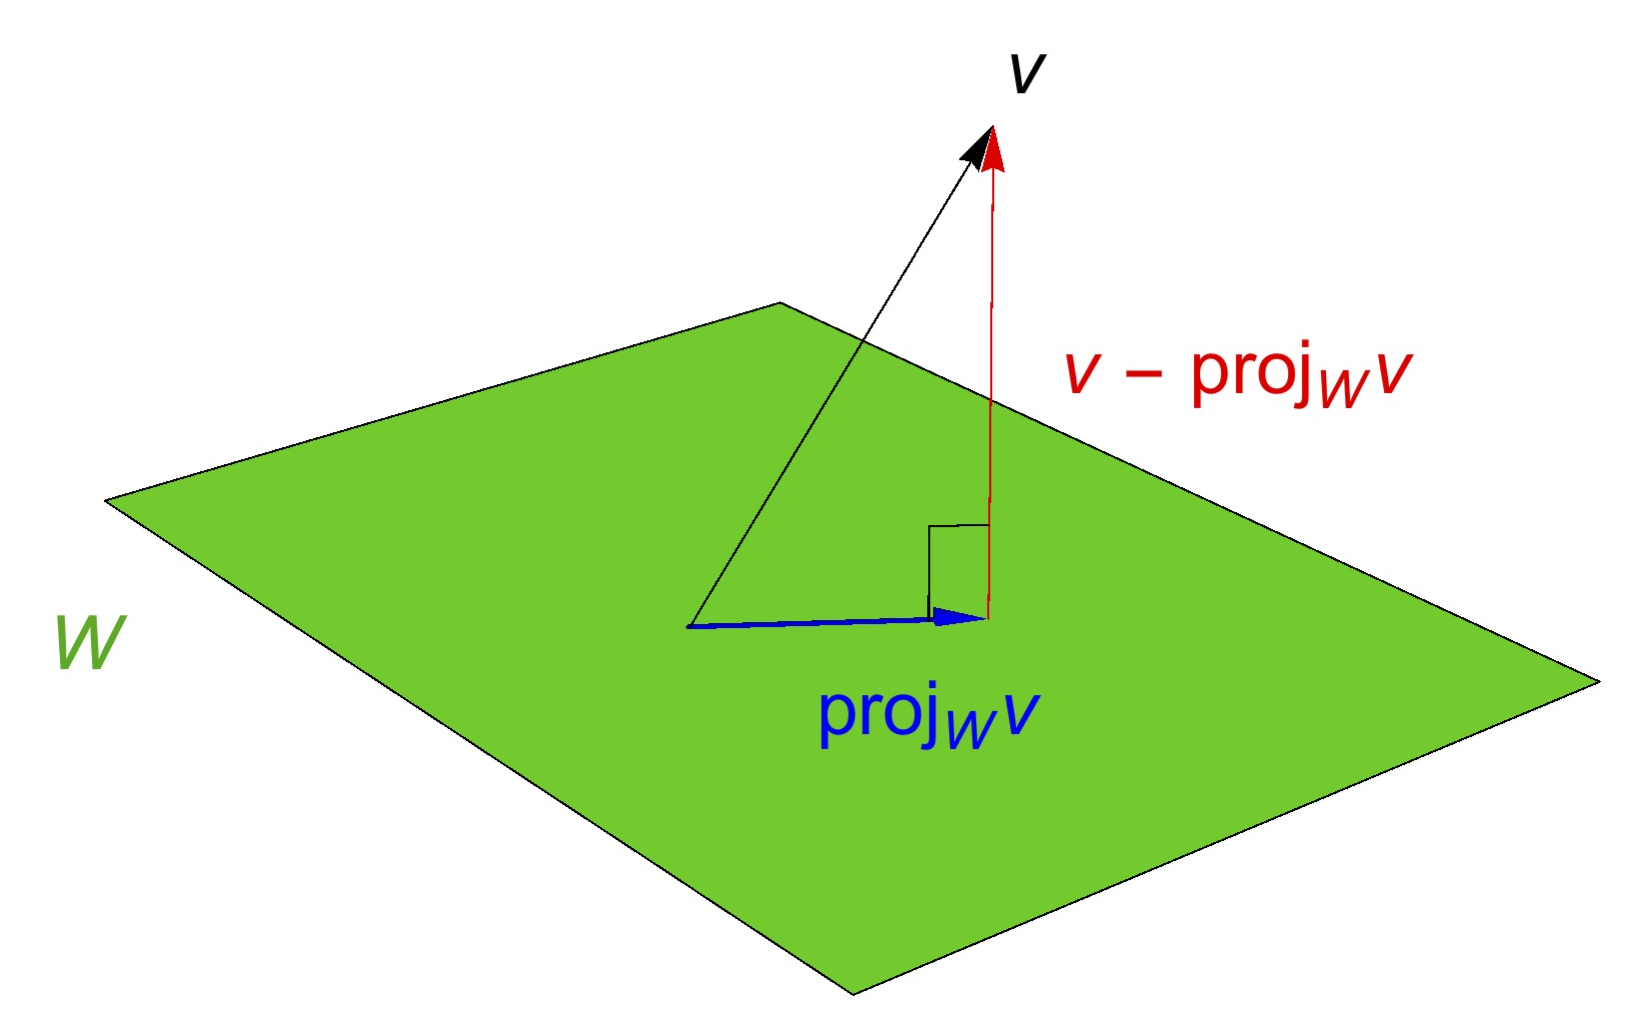
\includegraphics[scale=.2] {projW.jpg}~\\[1cm]
\end{center} 
\vglue-1cm
\caption{La projection orthogonale de $\vv$ sur le sous-espace $W$.}\label{figure:othogproj}\label{fig:19.1}
\end{figure}

Maintenant que la curiosité de votre esprit a été attisée, vous vous posez sans doute les deux questions suivantes :
\begin{enumerate}

\item {\it N'importe quel sous-espace admet-t-il une base orthogonale ?} Car la formule en a besoin...\label{goodquestion1}

\item {\it Si je calcule cette projection avec 2 bases orthogonales différentes, que se passe-t-il ? Je vais sûrement obtenir des réponses différentes, non ?\!? Du moins, les coordonnées seront différentes...}
\end{enumerate}
 
\medskip

Après avoir étudié un exemple, nous répondrons à la deuxième question; puis plus tard nous nous attaquerons à la première question, lorsque nous aurons introduit l'algorithme de Gram-Schmidt.


\begin{myexample}
Regardons à nouveau le sous-espace $W=\set{(x,y,z,w) \in \R^4 \st x-y-z+w=0}$. Par ce qui précède, nous savons que les 3 vecteurs $\ww_1=(1,1,1,1), \ww_2=(1,-1,1,-1)$ et $ \ww_3=(1,1,-1,-1)$ forment une base orthogonale pour $W$, et que le vecteur $\vv = (1,2,3,5) \notin W$ est projeté sur le vecteur :
$$
\proj_W(\vv) = \frac{11}4\ww_1 - \frac34\ww_2 - \frac{5}{4}\ww_3=\frac14\mat{3\\ 9\\ 13\\ 19}\in W\,.
$$
(Si vous le souhaitez, vous pouvez vérifier que $\frac14(3, 9, 13, 19)\in W$; il suffit de montrer que ce vecteur satisfait l'équation $x-y-z+w=0$.)

{\bf N.B.:} \underbar{Vous ne devez pas changer la longueur du vecteur de cette réponse!} C'est-à-dire : il ne faut pas changer le coefficient $\frac14$ devant le vecteur. Il s'agit d'une erreur très, très courante à ce stade. Vous pouvez changer la longueur des vecteurs d'une base orthogonale, mais vous ne pouvez pas changer la longueur du vecteur projection, c'est une réponse fixe !

De plus, comme le suggère la Figure \ref{figure:othogproj},
le vecteur $\vv-\proj_W(\vv)=\frac14(1, -1, -1, 1)$ est en fait orthogonal à tout vecteur de $W$ (cette idée était déjà le cas dans $\R^3$, voir pages \pageref{propOrthogProj} et \pageref{orthoprojonvector}). Pour montrer cela, regardez à nouveau l'équation définissant $W$ : elle nous dit que $(x,y,z,w) \in W$ si et seulement si 
$$ 0=x-y-z+w=(x,y,z,w)\cdot(1, -1, -1, 1)\,.$$ Donc tout vecteur de $W$ {\it est} bien orthogonal à $\vv-\proj_W(\vv)$.
\end{myexample}

\standout{\it Ceci arrive toujours : le vecteur $\vv-\proj_W(\vv)$ est bien orthogonal à n'importe quel vecteur de $W$. De plus, comme les Figures \ref{orthoprojonvector} et \ref{figure:othogproj} le suggèrent, le vecteur $\proj_W(\vv)$ est en fait {\it le  vecteur le plus proche de $\vv$ parmi tous les vecteurs de $W$}. 

Une autre façon de le dire: le vecteur $\proj_W(\vv)$ est la {\it meilleure approximation de $\vv$ par un vecteur de $W$}.}

Montrons que ceci est vrai.
\begin{theorem}[La meilleure approximation]\index{projection orthogonale} \label{orthogproj}
Soit $W$ un sous-espace de $\R^n$ et soit $\vv \in \R^n$. Alors on a :

\begin{enumerate}[(1)]
\item $\proj_W(\vv) \in W$;
\item $\vv - \proj_W(\vv)$ est orthogonal \`a tout vecteur de $W$;
\item $\proj_W(\vv)$ est la meilleur approximation de $\vv$ par un vecteur de $W$;
\item le vecteur $\proj_W(\vv)$ est l'\underbar{unique} vecteur de $\R^n$ qui satisfait (1) et (2).
\end{enumerate} 

\end{theorem}



Remarque : la propriété (4) nous dit que la projection orthogonale
est uniquement caractérisée par les deux propriétés (1) et (2).


\begin{proof} 
\begin{enumerate}[(1)]
	\item Cette partie est facile à montrer : utilisez la formule dans la Définition \ref{projdef}. Le vecteur $\proj_W(\vv)$ est une combinaison linéaire de vecteurs du sous-espace $W$ et doit donc appartenir à $W$.

	\item Comment pourrions-nous montrer qu'un vecteur est orthogonal à chaque vecteur de $W$ ? Il y a une infinité de vecteurs dans un sous-espace (du moins dans la plupart d'entre eux)...  C'est là que les bases vont être très utiles : pour «~rendre fini l'infini~» ! 

Supposons donc que $\{\ww_1, \cdots, \ww_m\}$ soit la base orthogonale pour $W$ que nous avons utilisée pour définir la projection. Chaque vecteur $\uu\in W$ est alors combinaison linéaire des $\ww_1, \cdots, \ww_m $; c'est-à-dire que $u$ s'écrit
 $$\uu =a_1 \ww_1 +\cdots + a_m \ww_m$$ pour certains scalaires $a_1, \cdots, a_m\in\R$. 
 Donc si l'on arrive à montrer que $(\vv-\proj_W(\vv))\cdot \ww_i=0$ pour tout $1\le i \le m$, alors le tour est joué (en notant $\ww=\proj_W(\vv)$ dans ce qui suit) :
\vglue-.4cm
\begin{align*} 
(\vv-\ww) \cdot \uu &=(\vv-\ww)\cdot (a_1 \ww_1 +\cdots + a_m \ww_m) \\
&=a_1((\vv-\ww)\cdot \ww_1) +\cdots +a_1((\vv-\ww)\cdot \ww_m)\\
&=a_1(0) +\cdots +a_1(0)\\&=0\,.
\end{align*}
(Notez que nous n'avons utilisé qu'une seule propriété de $\{\ww_1, \cdots, \ww_m\}$ : le fait qu'il engendre $W$. Donc en fait, on a même montré quelque chose de plus général : si un vecteur $\vv$ est orthogonal à un {\it ensemble g\'en\'erateur} de $W$, alors $\vv$ est orthogonal à tout vecteur du un sous-espace $W$ !)
Il reste donc à montrer que $(\vv-\ww)\cdot \ww_i=0$ pour tout $1\le i \le m$. On calcule : 
\begin{align*}
 (\vv-\ww)\cdot\ww_i  &=
(\vv - (\frac{\vv\cdot \ww_1}{\Vert \ww_1\Vert^2}\ww_1 + \cdots 
+ 
\frac{\vv\cdot \ww_m}{\Vert \ww_m\Vert^2}\ww_m))\cdot \ww_i \\
 &= \vv \cdot \ww_i - \frac{\vv\cdot \ww_1}{\Vert \ww_1\Vert^2}\ww_1 \cdot \ww_i - \cdots - \frac{\vv\cdot \ww_m}{\Vert \ww_m\Vert^2}\ww_m \cdot \ww_i\\
&= \vv \cdot \ww_i - \frac{\vv\cdot \ww_i}{\Vert \ww_i\Vert^2}\ww_i \cdot \ww_i
\end{align*}

puisque tous les autres produits scalaires entre $\ww_i$ et $\ww_j$ sont nuls ;
et ce dernier terme donne :
$$
 = \vv \cdot \ww_i - \frac{\vv\cdot \ww_i}{\Vert \ww_i\Vert^2}\Vert \ww_i \Vert^2 = 0\,.
$$
Ceci est vrai pour chaque $i = 1,2,\cdots, m$, et nous pouvons donc conclure que $\vv-\ww$ est orthogonal à tout vecteur de $W$, ce qui montre que (2) est vrai.


	\item On pose comme précédemment $\ww = \proj_W(\vv)$.  Pour prouver que c'est le vecteur le plus proche
dans $W$ de $\vv$, soit $\ww' \in W$ un autre vecteur quelconque dans $W$.
Alors on a
$$
\Vert \vv- \ww' \Vert^2 = \Vert (\vv - \ww) + (\ww - \ww') \Vert^2
$$
Or, d'une part $\vv-\ww$ est orthogonal à tout vecteur de $W$, et d'autre part $\ww - \ww'$ est dans $W$ (puisque $W$ est un sous-espace et que $\ww$ et $\ww'$ appartiennent tous deux à $W$). Donc les deux vecteurs $\vv - \ww$ et $\ww - \ww'$
sont orthogonaux, et par le Théorème de Pythagore (\ref{eqn:Pythag}) page \pageref{eqn:Pythag}, nous avons l'égalité:
$$
\Vert \vv- \ww' \Vert^2 = \Vert (\vv - \ww)\Vert^2 + \Vert(\ww - \ww') \Vert^2\,.
$$
Mais ceci est $\geq \Vert (\vv - \ww)\Vert^2$
car on a toujours $ \Vert(\ww - \ww') \Vert^2\geq 0$, et donc nous avons montré que (3) est vrai.

	\item Cette partie est également simple. Supposons maintenant que deux vecteurs $\ww,\ww'$ satisfont les propriétés (1) et (2) ci-dessus, à savoir :

\begin{itemize}
\item $\ww, \ww' \in W$
\item $\vv - \ww$ et $\vv-\ww'$ sont chacun orthogonal \`a tout vecteurs de $W$.
\end{itemize}

Alors, $\ww- \ww'\in W$ puisque $W$  est un sous-espace. Mais regardez : $$\ww- \ww'= (\vv-\ww')-(\vv - \ww).$$ Or, la somme -- ou la différence -- de deux vecteurs qui sont tous deux orthogonaux à chaque vecteur de $W$ sera à nouveau orthogonale à chaque vecteur de $W$. \footnote{Je ne sais pas pour vous, mais je commence à en avoir assez d'écrire \ \og est orthogonal à chaque vecteur de $W$\ \fg. Nous allons donc bientôt donner un nom à l'ensemble de tous les vecteurs orthogonaux à chaque vecteur de $W$. Nous l'appellerons $W^\perp$ --- voir Chapitre \ref{chapter:Fr_23-orthogcomp}.} Donc le vecteur $\ww- \ww'$ est orthogonal à chaque vecteur de $W$, y compris $\ww- \ww'$ lui-même ! Cependant, le seul vecteur orthogonal à lui-même est le vecteur nul, donc $\ww- \ww'=\zero$, ce qui donne bien l'unicité voulue $\ww= \ww'$.

Ceci montre bien qu'il n'existe qu'un seul vecteur ayant les propriétés (1) et (2) ci-dessus, à savoir $\proj_W(\vv)$.
\end{enumerate}
\end{proof}

Notez que la propriété (3) ci-dessus de la projection orthogonale est extrêmement utile dans de nombreux domaines. Elle constitue une partie importante de la base mathématique du traitement moderne du signal. Elle est utilisée dans presque toutes les méthodes quantitatives pour l'ajustement optimal de la courbe des données. Nous en présentons un exemple dans la Section \ref{leastsquares}, avec ce qu'on appelle l'\emph{approximation des moindres carrés}. 


L'idée de base est que nous disposons souvent d'un sous-espace $W$ (dans un espace vectoriel de signaux, par exemple) et d'un vecteur $\vv$ dont nous ne sommes pas certain qu'il appartienne à notre sous-espace $W$. Nous souhaitons ne traiter que les vecteurs de $W$\kern-2pt, donc nous projetons notre vecteur $\vv$ sur $W$ et nous traitons sa projection à la place de lui-même. 

Par exemple, pour faire simple, disons sur votre téléphone portable, lorsque vous prenez une photo et que vous souhaitez l'envoyer à un ami, la photo est capturée, stockée et traitée comme un vecteur dans un espace de grande dimension ($\R^n$ pour un certain nombre $n$ très grand). Cependant, au lieu d'envoyer toutes les entrées du vecteur, on projette le vecteur (orthogonalement) sur un sous-espace beaucoup plus petit -- avec une base orthogonale propre au protocole utilisé -- et ensuite on transmet d'un téléphone à l'autre uniquement les coefficients de Fourier, lesquels sont beaucoup moins nombreux que les $n$ coefficients de l'espace de départ. Sur le téléphone de votre ami qui reçoit les coefficients de Fourier, on peut ensuite utiliser la même base orthogonale pour restituer la projection à l'aide des coefficients de Fourier, obtenant ainsi une approximation (plus ou moins précise, en fonction de $\dim W$ et de $n$) de l'image que vous aviez envoyée.

La partie (4) ci-dessus semble inoffensive jusqu'à ce qu'on se rappelle que la Définition \ref{projdef} (page \pageref{projdef}) {\it semblait} dépendre d'un choix de base orthogonale. Donc en fait, ce que la partie (4) dit, c'est que les différentes formules que l'on obtient en utilisant différentes bases orthogonales pour calculer la projection donnent toutes exactement la même réponse finale! Wow ! Ceci répond à notre deuxième question !

\section{Bases orthogonales : l'algorithme de Gram-Schmidt}\label{section:Gram-Schmidt}

Jusqu'à présent, nous avons supposé implicitement que chaque sous-espace $W$ de $\R^n$ {\it admet} une base orthogonale. Est-ce vrai ? En fait oui, et encore même mieux, il existe un algorithme simple qui transforme n'importe quelle base de $W$ en une base orthogonale de $W$ !\!!


 

Supposons que $\set{\uu_1, \cdots, \uu_m }$ soit une base quelconque de $W$.  Nous voulons trouver une base orthogonale pour $W$.

L'idée géométrique est assez simple : commencez avec votre premier vecteur $\ww_1 = \uu_1$.
Prenez ensuite $\ww_2 = \uu_2 - \proj_{\uu_1}(\uu_2)$. Par ce qui précède, vous avez que $\ww_2$ est orthogonal à $\ww_1$, et on voit que $\ww_1$ appartient bien à $W$ (il est même combinaison linéaire de $\uu_1$
et $\uu_2$).  Continuez ainsi de suite à construire $\ww_i$ en soustrayant $\uu_i$ à sa projection sur le sous-espace $\spn\{\ww_1, \dots, \ww_{i-1}\}$. Lorsque vous aurez atteint $i=m=\dim(W)$, vous aurez construit une base orthogonale $\{\ww_1, \dots, \ww_{m}\}$ de $W$.

\begin{theorem}[L'algorithme de Gram-Schmidt]\index{algorithme de Gram-Schmidt}\label{theorem:GS}
Soit $\set{\uu_1, \cdots, \uu_m }$ une base {\it quelconque} de $W$.  On d\'efinit les vecteurs et sous-espaces suivants:
\begin{itemize}
\item $\ww_1 = \uu_1$  and $V_1 = \spn\{\ww_1\}$;
\item $\ww_2 = \uu_2 - \proj_{V_1}(\uu_2)$ and $V_2 = \spn\{\ww_1,\ww_2\}$;
\item $\ww_3 = \uu_3 - \proj_{V_2}(\uu_3)$ and $V_3 = \spn\{\ww_1,\ww_2,\ww_3\}$;
\item $\cdots$
\item $\ww_m = \uu_m - \proj_{V_{m-1}}(\uu_m)$ et $V_m = \spn\{\ww_1,\cdots,\ww_m\}$.
\end{itemize}
Alors $W = V_m$ et   
$\{\ww_1,\cdots,\ww_m\}$ est une base orthogonale pour $W$.

\medskip
Exprimés plus en détail, les vecteurs sont :

\begin{itemize}
\item $\ww_1 = \uu_1$;
\item $\ww_2 = \uu_2 - \proj_{\ww_1}(\uu_2)$;
\item $\ww_3 = \uu_3 - \proj_{\ww_1}(\uu_3)-\proj_{\ww_2}(\uu_3)$;
\item $\cdots$
\item $\ww_m = \uu_m - \sum_{i=1}^{m-1}\proj_{\ww_{i}}(\uu_m)$.
\end{itemize}
Alors $\{\ww_1,\cdots,\ww_m\}$ est une base orthogonale pour $W$.

Enfin, on peut normaliser cette base (\textit{i.e.} rendre la norme de chaque vecteur de la base \'egale \`a 1) en divisant les vecteurs par leur norme. On a alors
une base orthonormée de $W$.
\end{theorem}

Remarquez qu'à chaque étape, les vecteurs de l'ensemble g\'en\'erateur de $V_i$ sont orthogonaux, ce qui signifie qu'il est facile de calculer la projection sur
$V_k$.  En fait, on a $V_k = \spn\{\uu_1 , \cdots, \uu_k\}$ ; c'est à dire l'enveloppe lin\'eaire engendr\'ee par $\{\ww_1, \dots, \ww_k\}$ est la même que celle engendr\'ee par les vecteurs de l'ensemble original $\{\uu_1, \dots, \uu_k\}$, pour n'importe quel $1\leq k \leq m$.

\medskip
Par ailleurs, notez qu'on pourrait commencer par un  ensemble \emph{g\'en\'erateur} $\set{\uu_1,\cdots, \uu_p}$ de $W$ (plutôt qu'une base) et appliquer le même algorithme de Gram-Schmidt. Alors on obtiendrait un ensemble $\{\ww_1,\cdots,\ww_p\}$, et les  vecteurs {\it non nuls} de cet ensemble formeraient une base orthogonale de $W$ ! Voir Exercice~\ref{prob19.6}.

\begin{myexample}\label{example:GS} Exécutons l'algorithme de Gram-Schmidt sur l'ensemble 
$$\{ (1,0,0,1), (1,1,1,0), (2,1,-1,1)\}\,.
$$

(Vous pouvez vérifier que c'est bien une base du sous-espace $W=\sp{ (1,0,0,1), (1,1,1,0), (2,1,-1,1)}=\set{(x,y,z,w)\in \R^4\st x - y - w = 0}$.\footnote{Nous avons vu comment faire cela à la fin du Chapitre \ref{chapter:Fr_17-homogsystems}.})


On commence par poser
$$
\ww_1 = (1,0,0,1)\,,
$$
puis on calcule
\begin{align*}
\ww_2 &= \uu_2 - \proj_{\ww_1}(\uu_2)\\
&= \uu_2 - \frac{\uu_2\cdot \ww_1}{\|\ww_1\|^2}\ww_1 \\
&= (1,1,1,0) - \frac{1}{2}(1,0,0,1) = \left(\frac12,1,1,-\frac12\right). 
\end{align*}

(Avant de continuer, c'est toujours une bonne idée de vérifier qu'on a bien $\ww_1\cdot \ww_2 =0$ ! C'est pour se rassurer un peu qu'on n'a pas fait d'erreur de calcul... Vérifiez-le !).
Et, dans cet exemple, il ne reste qu'une autre étape \`a faire:

\begin{align*}
\ww_3 &= \uu_3 - \frac{\uu_3\cdot \ww_1}{\|\ww_1\|^2}\ww_1 - \frac{\uu_3\cdot \ww_2}{\|\ww_2\|^2}\ww_2\\
&= (2,1,-1,1) - \frac{3}{2} (1,0,0,1) - \frac{1/2}{5/2}
\left(\frac12,1,1,-\frac12\right) \\
&= (2,1,-1,1) -\left(\frac32,0,0,\frac32\right) - \left(\frac1{10}, \frac15
 , \frac15, -\frac1{10}\right)\\
&= \frac25(1, 2 , -3 , -1)\,.
\end{align*}
Nous pouvons alors voir que $\{\ww_1,\ww_2,\ww_3\}$ est effectivement orthogonal (c'est toujours une bonne idée de le vérifier). \footnote{Aussi, si vous avez le temps, c'est aussi une très bonne idée de vérifier que vos vecteurs $\ww_1,\ww_2,\ww_3$ appartiennent bien à $W$ -- ce qui est bien le cas ici ! Ici, c'est facile, car nous avons une description simple de $W$, à savoir  $W=\set{(x,y,z,w)\in \R^4\st x - y - w = 0}$, mais dans d'autres cas cette vérification peut être un peu plus longue...}  De plus,
en regardant nos calculs plus attentivement, nous pouvons voir qu'en effet,
chaque vecteur $\ww_i$ est bien dans l'enveloppe lin\'eaire engendr\'ee par les vecteurs originaux $\uu_1, \dots, \uu_i$. 
La base orthogonale résultante est alors la suivante :
$$
\left\{ (1,0,0,1), \frac12(1,2,2,-1), \frac25(1,2,-3,-1)\right\}\,.
$$  

\begin{remark} Nous simplifierons souvent nos résultats à la fin en multipliant les vecteurs 
$\ww_i$ par un scalaire convenable, de fa\c{c}on \`a éviter les fractions. Dans l'exemple pr\'ec\'edent, on peut donner le résultat suivant :
$$
\{ (1,0,0,1), (1,2,2,-1), (1,2,-3,-1)\}\,,
$$
lequel est bien un ensemble orthogonal, et il a le bon goût de ne pas avoir de fractions. Donc il
pourrait être
plus facile à utiliser si vous deviez calculer une autre projection par exemple.
\end{remark}

\medskip
Enfin, si l'on veut vraiment une base \emph{orthonormée}, il faut diviser chacun de ces vecteurs par leur norme.  Pour l'exemple pr\'ec\'edent, comme 
$
\Vert (1,0,0,1) \Vert = \sqrt{2}$,  que $\Vert  (1,2,2,-1) \Vert =   \sqrt{10}$, et que $ \Vert  (1,2,-3,-1) \Vert =   \sqrt{15} $, on obtient la base orthonormée suivante :
$$
\left\{ \frac{\sqrt{2}}{2}(1,0,0,1), \frac{\sqrt{10}}{ 10 }(1,2,2,-1), \frac{\sqrt{15}}{15}(1,2,-3,-1)\right\}\,.
$$
(V\'erifiez-le!) Par contre, pour les bases orthonormées, on ne peut pas changer la norme à notre guise pour enlever les fractions puisqu'on veut que la norme de chaque vecteur soit égale à $1$ (c'est une contrainte assez forte !).
\end{myexample}



\begin{myexample}\label{Wagain} Calculez la meilleure approximation de $\vv = (1,2,3,4)$ dans $W$, où
$$
W = \spn\{(1,0,0,1), (1,1,1,0), (2,1,-1,1)\}=\set{(x,y,z,w)\in \R^4\st x - y - w = 0}\,.
$$

Utilisons l'exemple précédent.  Nous savons déjà qu'une
base orthogonale pour $W$ est 
$$
\{  (1,0,0,1),  (1,2,2,-1),  (1,2,-3,-1)\}\,.
$$
Notons ces vecteurs respectivement $\nn_1$, $\nn_2$, $\nn_3$.
On a alors :
\begin{align*}
\proj_W(\vv) &= \frac{\vv\cdot\nn_1}{\|\nn_1\|^2} \nn_1 +  \frac{\vv\cdot\nn_2}{\|\nn_2\|^2} \nn_2 + \frac{\vv\cdot\nn_3}{\|\nn_3\|^2} \nn_3 \\  
&= \frac{5}{2}  (1,0,0,1) + \frac{7}{10} (1,2,2,-1)  -\frac{8}{15}(1,2,-3,-1)\\
&=  \frac{1}{3}(8,1,3,7).
\end{align*}

Si vous avez le temps, vérifiez que la réponse appartient bien à $W$. Ici c'est facile puisque nous avons une description simple de $W$. \footnote{ Si vous avez le temps, vous devriez également vérifier que le vecteur $(1,2,3,4)-\frac{1}{3}(8,1,3,7)=\frac13(-5,5,0,5)$ est orthogonal à tout vecteur de $W$. C'est bien le cas, puisque $\frac13(-5,5,0,5)\cdot (x,y,z,w)=-\frac53 (x-y-w)=0 $ \`a chaque fois que $(x,y,z,w)\in W$ ! }
\end{myexample}



\section*{Exercices}
\addcontentsline{toc}{section}{Exercices}
 

\begin{prob} \label{prob19.1} Dans chaque cas, trouvez les coefficients de Fourier (coordonn\'ees) du vecteur $\vv$ par rapport à la base orthogonale $\mathcal B$ donnée de l'espace vectoriel $W$ indiqué.
\medskip

\begin{enumerate}[a)]
\item  $\vv=(1,2,3)$, $\mathcal B = \set{(1,0,1),(-1,0,1), (0,1,0) }$, $W=\R^3$.
\medskip
 
\item\sov~ $\vv=(1,2,3)$, $\mathcal B = \set{(1, 2 , 3 ),(-5, 4, -1),(1, 1, -1)}$, $W=\R^3$.
\medskip
 
\item  $\vv=(1,2,3)$, $\mathcal B = \set{(1, 0, 1),(-1, 2, 1)}$, $$W=\set{(x,y,z)\in\R^3 \st x+y-z=0}.$$
 
 
\item\sov~$\vv=(4,-5,0)$, $\mathcal B = \set{(-1, 0, 5),(10, 13, 2)}$, $$W=\set{(x,y,z)\in\R^3 \st 5x-4y+z=0}.$$
 
 
\item $\vv=(1,1,1,1)$,  $\mathcal B =\set{(1, 0, 1, 1), (0, 1, 0, 0), (0, 0, 1, -1)}$, $$W=\set{(x,y,z, w)\in\R^4 \st x-w=0}.$$
\medskip
 
\item\sov~$\vv=(1,0,1,2)$,  $\mathcal B =\set{(1, 0, 1, 1), (0, 1, 0, 0), (0, 0, 1, -1),(1, 0, 0, -1)}$, $W= \R^4$.
\medskip
 
\end{enumerate}

\end{prob} \begin{prob} \label{prob19.2} Trouvez la formule de la projection orthogonale sur les sous-espaces des questions c), d)~\sov~et e) ci-dessus.

\end{prob} \begin{prob} \label{prob19.3} Appliquez l'algorithme de Gram-Schmidt à chacun des ensembles LI suivants (pour obtenir un ensemble orthogonal), et vérifiez que l'ensemble de vecteurs que vous obtenez est bien orthogonal.
\medskip
\begin{enumerate}[a)]
\item $\set{(1,1,0),(2,0,3)}$.
\medskip
 
\item\sov~$\set{(1, 0, 0, 1),(0, 1, 0, -1),(0, 0, 1, -1)}$.
\medskip
 
\item $\set{(1, 1, 1, 1),(0, 1, 0, 0),(0, 0, 1, -1)}$.
\medskip
 
\item\sov~$\set{(1, 1, 0),(1, 0, 2),(1, 2, 1)}$.
\medskip
 
\end{enumerate}
\end{prob} \begin{prob} \label{prob19.4} Trouvez une base orthogonale pour chacun des sous-espaces suivants et vérifiez que votre base est bien orthogonale. (Astuce : tout d'abord, trouvez une base quelconque de manière standard, puis appliquez l'algorithme de Gram-Schmidt pour en trouver un orthogonale.)
\medskip
\begin{enumerate}[a)]
\item $W=\set{(x,y,z)\in\R^3 \st x+y+z=0}$.
\medskip
 
\item\sov~
 $U=\set{(x,y,z, w)\in\R^4 \st x+y-w=0}$.\medskip
 
\item $X=\set{(x,y,z, w)\in\R^4 \st x+y-w=0 \, \text{ et } \, z+y=0}$.
\medskip
 
\item\sov~$V=\ker \bmatrix 1 & 2 & -1 & -1 \\
 2 & 4 & -1 & 3 \\
 -3 & -6 & 1 & -7 \endbmatrix$.
\medskip
 
\end{enumerate}

\end{prob} \begin{prob} \label{prob19.5} Dans chaque cas, trouvez la meilleure approximation du vecteur $\vv$ donné par un vecteur $\ww$ du sous-espace $W$ donné. \medskip
\begin{enumerate}[a)]
\item  $\vv=(1,1,1)$,  $W=\set{(x,y,z)\in\R^3 \st x+y-z=0}$.
\medskip
 
\item\sov~$\vv=(1,1,1)$,   $W=\set{(x,y,z)\in\R^3 \st 5x-4y+z=0}$.
\medskip
 
\item  $\vv=(1,1,1,2)$,   $W=\set{(x,y,z, w)\in\R^4 \st x-w=0}$.
\medskip
 
\end{enumerate}
\end{prob} \begin{prob} \label{prob19.6}  Pour chacun des énoncés suivants, indiquez s'il est (toujours) vrai ou s'il est (possiblement) faux.   
   \smallskip    
\begin{enumerate}[$\bullet$]
\item Si vous dites que l'\'enonc\'e est faux, donnez un contre-exemple.   
\item Si vous dites que l'\'enonc\'e est vrai, donnez une explication claire - en citant un théorème ou en donnant une {\it preuve valide dans tous les cas}. 
\end{enumerate}

\medskip
\begin{enumerate}[a)]
\item Tout ensemble orthogonal est linéairement indépendant.
\medskip
 
\item\sov~Tout ensemble linéairement indépendant est orthogonal.
\medskip
 
\item Pour trouver la projection orthogonale d'un vecteur $\vv$ sur un sous-espace $W$, il suffit d'utiliser une base quelconque de $W$ dans la formule de la Définition\ref{projdef} (page~\pageref{projdef}).  
\medskip
 
\item\sov~Lorsque l'on cherche la projection orthogonale d'un vecteur $\vv$ sur un sous-espace $W$, une fois la réponse obtenue, on peut la multiplier la réponse par un  scalaire convenable pour éliminer les fractions.
\medskip
 
\item Lorsque l'on applique l'algorithme de Gram-Schmidt à une base, à chaque étape, il est bon de simplifier le vecteur obtenu en multipliant par un scalaire pour éliminer les fractions.
\medskip
  
\item\sov~Lorsque l'on recherche la projection orthogonale d'un vecteur $\vv$ sur un sous-espace $W$, si l'on utilise différentes bases orthogonales de $W$ dans la formule de la Définition~\ref{projdef} (page~\pageref{projdef}), alors on aura possiblement des réponses différentes.
\medskip
 
\item Si $\proj_W(\vv)$ désigne la projection orthogonale d'un vecteur $\vv$ sur un sous-espace $W$, alors le vecteur $\vv-\proj_W(\vv)$ est toujours orthogonal à tout vecteur de $W$.
\medskip
 
\item\sov~Pour vérifier qu'un vecteur, disons $\uu$, est orthogonal à tout vecteur dans $W$, il suffit de vérifier que $\uu$ est orthogonal à tout vecteur d'une base de $W$.
\medskip
 
\item$^{\ast \ast}$ Si l'on applique l'algorithme de Gram-Schmidt à un {\it ensemble g\'en\'erateur} $\set{\ww_1, \dots , \ww_p}$ d'un sous-espace $W$ plutôt qu'à une base de $W$, et si l'on obtient un vecteur nul \`a l'\'etape $k$, cela signifie que $\ww_k \in \sp{\ww_1, \dots , \ww_{k-1}}$.
\medskip
 
\item $^{\ast \ast}$ Si vous appliquez l'algorithme de Gram-Schmidt à un {\it ensemble g\'en\'erateur} $\set{\ww_1, \dots , \ww_m}$ d'un sous-espace $W$ plutôt qu'à une base de $W$, et que vous écartez tous les vecteurs nuls qui apparaissent au cours du processus, alors vous obtiendrez bien au final une base orthogonale pour $W$.
\medskip
 
\end{enumerate}
\end{prob}
  

\chapter{Complément orthogonal, applications}
\label{chapter:Fr_23-orthogcomp}

\section{Complément orthogonal}
Dans le chapitre pr\'ec\'edent, nous avons vu une propriété importante de la projection orthogonale : en notant $\proj_W(\vv)$ la projection d'un vecteur $\vv\in V$ orthogonalement sur un sous-espace $W\subseteq V$, on a que le vecteur $\vv-\proj_W(\vv)$ est {\it orthogonal à tout vecteur de $W$}. Ceci suggère la définition suivante.



\begin{definition}
Soit $U$ un sous-espace de $\R^n$.  Le \defn{complément orthogonal} de $U$
est l'ensemble noté $U^\perp$ et défini par :
$$
U^\perp = \set{ \vv \in \R^n \st\uu \cdot \vv = 0 \textrm{\; pour tout $\uu\in U$}}.
$$
Voir une illustration dans la Figure \ref{figure:Uperp}. (Remarque : le complément orthogonal de $U$ est unique.)
\end{definition}

\begin{figure}
\begin{center}
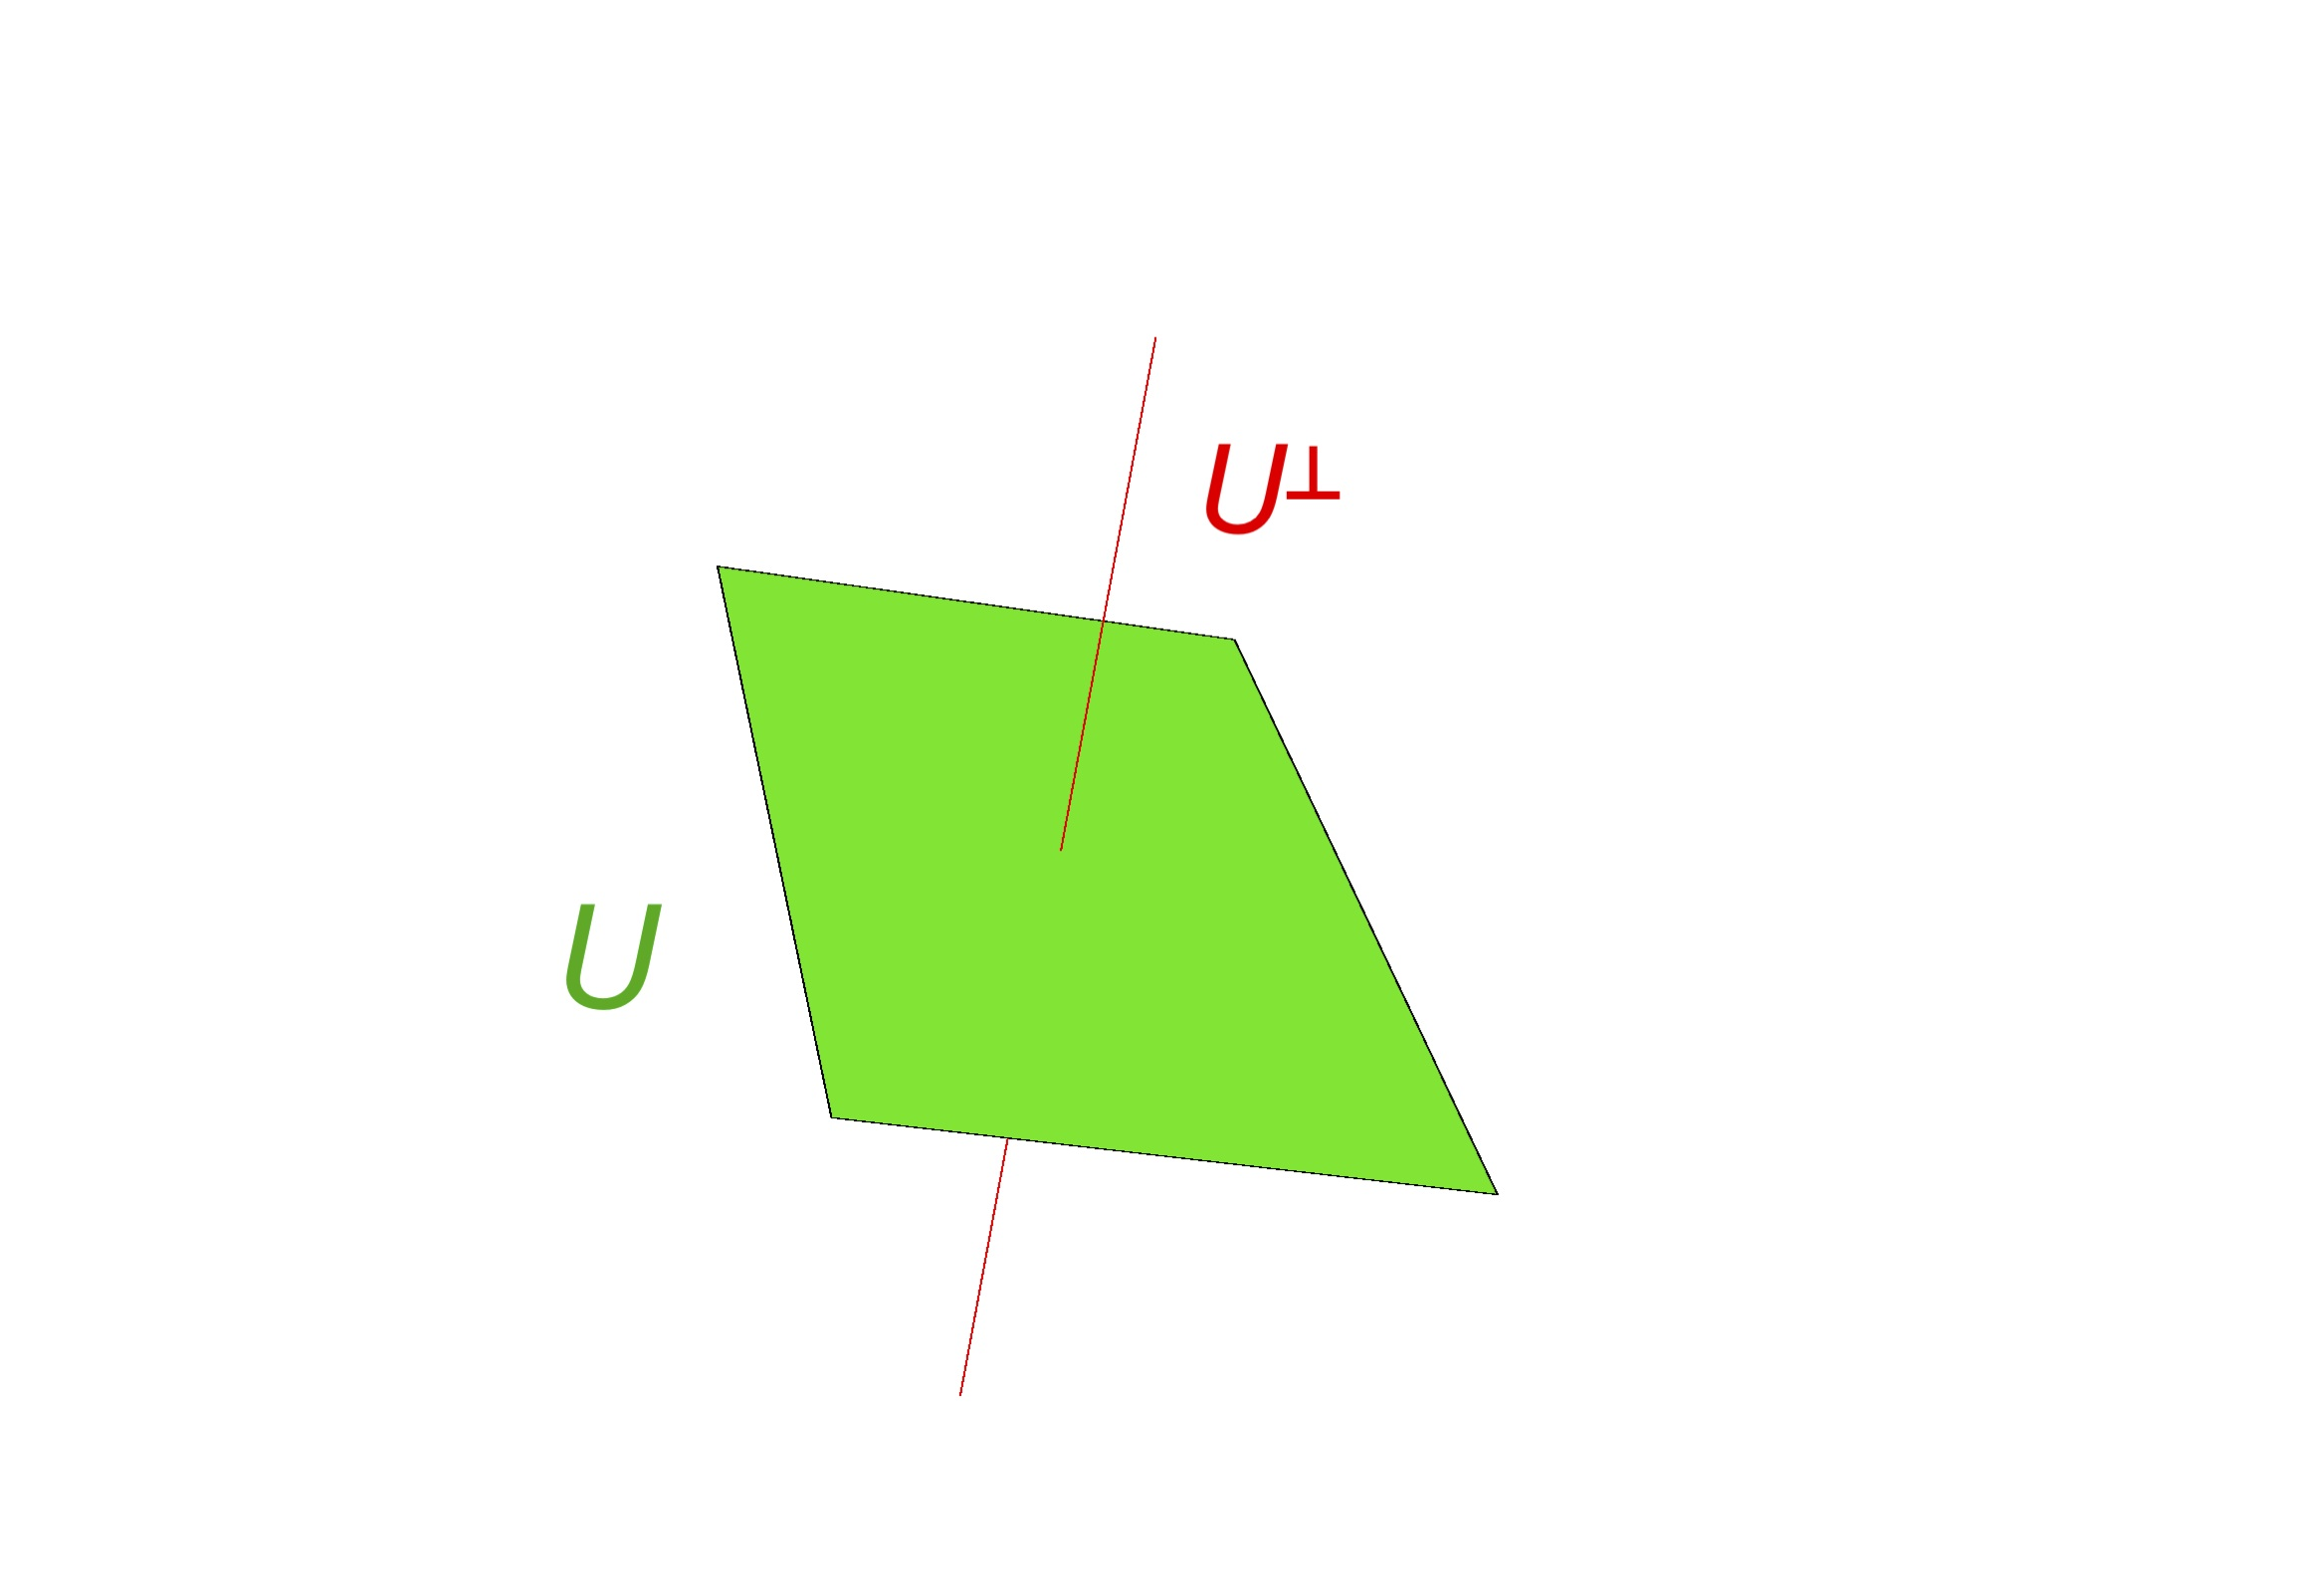
\includegraphics[scale=.5] {Uperp.jpg}~
\end{center} 
\vglue-.5cm
\caption{Le plan $U$ et son complément orthogonal.}\label{figure:Uperp}
\end{figure}

\begin{myexample}


Soit le sous-espace $U = \spn\{ (1,0,3), (0,1,2)\}$. Nous savons que $U$ est un plan passant par l'origine, et il est défini par le vecteur normal $(1,0,3) \times (0,1,2)=(-3, -2, 1)$. (On a calculé le produit vectorielle, cf. les chapitres précédents.) 

Un vecteur $\vv\in\R^3$ est donc orthogonal à $U$ si et seulement s'il est parallèle à $(-3, -2, 1)$. Ainsi,  

$$U^\perp=\sp{(-3, -2, 1)}.$$ 

En d'autres termes, l'ensemble $U^\perp$ est aussi un sous-espace : c'est la droite passant par l'origine et de vecteur directeur $(-3, -2, 1)$.
\end{myexample}


\begin{myexample}
Soit $U$ le sous-espace de $\R^4$ défini par $U=\sp{(1,-1,0,-1)} $. 

Rappel : un vecteur est $\vv\in\R^4$ orthogonal à tout vecteur de $U$ si et seulement si $\vv$ est orthogonal aux vecteurs d'une base de $U$ (voir la preuve du Théorème~\ref{orthogproj} page \pageref{orthogproj}). En d'autres termes, un vecteur $\vv=(x,y,z,w)\in\R^4$ appartient à $U^\perp$ si et seulement si 
$$(x,y,z,w)\cdot (1,-1,0,-1)=0.$$ Mais le membre de gauche est égal à $ x - y - w$, donc on en déduit l'expression de $U^\perp$ :
$$U^\perp = \set{(x,y,z,w)\in \R^4\st x - y - w=0}\,.
$$
(Vous reconnaîtrez peut-être le sous-espace comme $W$ qu'on avait étudié \`a la page~\pageref{example:GS} parmi les deux derniers exemples du chapitre précédent.)
\end{myexample}

Qu'en est-il de $W^\perp$ si $W=U^\perp$ de l'exemple pr\'ec\'edent ?\medskip

\begin{myexample}
Soit $W=\set{(x,y,z,w)\in \R^4\st x - y - w = 0}$.

Nous savons que qu'un vecteur $\vv \in \R^4$ appartient à $W^\perp$ si et seulement si $\vv$ est orthogonal à tout vecteur d'une base de $W$. Nous connaissons plusieurs bases de $W$ : par exemple, à partir de l'exemple \`a la page~\pageref{Wagain}, nous savons que l'ensemble suivant est une base de $W$ :
$$ \set{\vv_1=(1,0,0,1), \vv_2=(1,1,1,0), \vv_3=(2,1,-1,1)}\,.$$ 
Donc nous devons juste trouver tous les $\vv$ de $\R^4$ tels que les trois équations suivantes sont vérifiées :
\begin{align*}
\notag \vv_1\cdot \vv&=0,\\
\vv_2\cdot \vv&=0, \tag{$\ast$}\label{eqn:aaa}\\
\notag \vv_3\cdot \vv&=0\,.
  \end{align*}

Nous avons déjà vu ce genre de chose auparavant ! Vous souvenez-vous de la Remarque~\ref{NullperpRow} à la page \pageref{NullperpRow} ? Elle disait en partie que pour une matrice $A$ donnée, un vecteur $\vv$ est orthogonal à chaque ligne de $A$ si et seulement si $\vv$ appartient à $\ker(A)$.

Or, en prenant la matrice $  A=\scriptsize  \bmatrix ~&\vv_1&~\\&\vv_2 \\&\vv_3\endbmatrix$ définie par blocs de lignes, on voit que les trois équations \eqref{eqn:aaa} sont satisfaites si et seulement si $\vv$ est orthogonal aux lignes de $A$, et donc par ce qu'on a dit ci-dessus, c'est équivalent à chercher $\vv$ dans le noyau $\ker(A)$. Ceci nous dit que $W^\perp = ker(A)$.
Calculons donc $\ker(A)$ :
$$W^\perp = \ker(A)=\ker \bmatrix  1&0&0&1\\1&1&1&0\\2&1&-1&1\endbmatrix =\ker\bmatrix  1 & 0 & 0 & 1 \\
 0 & 1 & 0 & -1 \\
 0 & 0 & 1 & 0 \\\endbmatrix=\set{(-s,s,0,s)\st s\in \R}\,.$$
Donc le singleton $\set{(-1,1,0,1)}$ est une base de $\ker(A)= W^\perp$, et on trouve que $W^\perp = U$.
\end{myexample}

Au final, avec les deux exemples précédents, nous avons les relations $W=U^\perp$ et $W^\perp = U$. Donc nous aboutissons à l'égalité suivantes :
$$(U^\perp)^\perp=U~!$$  
Mais cette égalité est-elle toujours vraie pour tout sous-espace $U$ de $\R^n$ ?
OUI, c'est bien le cas, et d'autres r\'esultats sont également vrais :

\begin{theorem}[Propriétés du complément orthogonal]\index{propriétés du complément orthogonal}\label{orthogcompprop}
Soit $U$ un sous-espace de $\R^n$.  Alors :
\begin{enumerate}[(1)]
\item $U^\perp$ est un sous-espace de $\R^n$;
\item $(U^\perp)^\perp = U$;
\item et $\dim(U) + \dim(U^\perp) = n$.
\end{enumerate}
Lorsque deux sous-espaces $U$ et $V$ satisfont l'égalité $U = V^\perp$ (ou de manière équivalente
$V = U^\perp$), alors on dit qu'ils sont des \defn{compléments orthogonaux l'un de l'autre}.
\end{theorem}

\begin{proof}
\begin{enumerate}[(1)]
	\item On applique le test des sous-espaces.  Rappelons la définition de $U^\perp$ :
$$
U^\perp = \{ \vv \in \R^n \mid \uu \cdot \vv = 0 \textrm{\; pour tout $\uu\in U$}\,.
 \}
$$
(a) Puisque le vecteur nul $\zero$ est orthogonal à tous les vecteurs de $U$ (il est même orthogonal
à tout vecteur de $\R^n$ !), on a bien $\zero \in U^\perp$. 

(b) Supposons que $\vv, \ww\in U^\perp$.  Alors $\uu \cdot \vv= 0$ et $\uu \cdot \ww =0$ pour tout $\uu\in U$.  Est-ce que $\vv + \ww \in U^\perp$?  On calcule :
$$
\uu \cdot (\vv + \ww) = \uu \cdot \vv + \uu \cdot \ww = 0 + 0 = 0.
$$
Donc, c'est bon, on a bien la stabilité par addition : $\vv + \ww \in U^\perp$. 

(c) Supposons que $\vv \in U^\perp$ et que $k\in \R$.  Par définition, on a $\uu \cdot \vv = 0$ pour tout $\uu\in U$.
L\`a encore, on calcule :
$$
\uu \cdot (k\vv) = k\uu \cdot \vv = k (0) = 0\,,
$$
donc on a bien la stabilité par multiplication par un scalaire : $k\vv \in U^\perp$. 

D'o\`u $U^\perp$ satisfait les trois points $(a), (b), (c)$ du test des sous-espaces, et c'est donc bien un sous-espace de $\R^n$.


	\item[(3)] Soit $\{\uu_1,\ldots, \uu_k\}$ une base de $U$.
Considérez la matrice $ A=\scriptsize  \bmatrix ~&\uu_1&~\\&\vdots \\&\uu_k\endbmatrix$ dont les bloc de lignes sont les vecteurs de cette base.
Alors l'ensemble de tous les vecteurs $\vv$ orthogonaux à $U$
est exactement l'ensemble des vecteurs $\vv$ tels que $A\vv = \zero$
(en utilisant l'argument de l'exemple ci-dessus).  Donc $U^\perp = \ker(A)$.
Or, par le Théorème du rang on a :
$$
\dim(\row(A)) + \dim(\ker(A)) = n\,,
$$
et le terme de gauche est égal à $\dim(U) + \dim(U^\perp)$. D'où l'égalité voulue.

	\item[(2)] Posons $V = U^\perp$. C'est un sous-espace par (1)
et sa dimension est $n - \dim(U)$ par (3).   Nous voulons conclure que $U = V^\perp$.  Puisque tout vecteur de $U$ est en effet orthogonal à tout vecteur de $V$, il est vrai que $U \subseteq V^\perp$.  De plus, par (3), on a que:
$$\dim(V^\perp) = n- \dim(V) = n-(n-\dim(U)) = \dim(U)\,.$$  
En résumé, l'ensemble $U$ est un sous-espace de $V^\perp$ 
qui a la même dimension que $V^\perp$, donc il est nécessairement \'egal \`a $V^\perp$.
(On a utilisé le théorème qui dit que si un sous-espace n'est pas l'espace entier, alors il
doit avoir une dimension strictement inf\'erieure \`a celle du plus grand espace).
\end{enumerate}
\end{proof}

\begin{myprob}
Soit $A$ une matrice quelconque.  Montrez que $\row(A)$ et $\ker(A)$ sont toujours compléments orthogonaux l'un de l'autre. Montrez le même résultat pour $\im(A)$ et $\ker(A^T)$.  

\begin{mysol}

C'est une reprise de notre exemple pr\'ec\'edent dans un cadre plus général.
Supposons que $A$ soit une matrice $m \times n$.
Rappelons que $\ker(A)=\set{\xx \in \R^n\st A \xx=\zero}$.
Par définition de la multiplication matricielle, l'égalité $A\xx=\zero$ revient à
dire que le produit scalaire de chaque ligne de $A$ avec $\xx$ est égal à 0, donc $$\ker(A)=\set{\xx \in \R^n \st \xx \text{ est orthogonal à chaque ligne de } A}\,.$$ 

Puisque les lignes de $A$ engendrent $\row(A)$, on a donc que $\xx \in \ker(A)$ si et seulement si $\xx$ est orthogonal à tout vecteur de $\row(A)$. Ainsi $\ker(A)=\row(A)^\perp$ comme requis.

Pour voir que $\ker(A^T)=\im(A)^\perp$, utilisez l'égalité $\ker(A)=\row(A)^\perp$ et substituez $A$ par $A^\perp$ pour obtenir $\ker(A^T)=\row(A^T)^\perp$. Concluez alors en utilisant le fait que $\im(A)=\row(A^T)$.
\end{mysol}
\end{myprob}






\section{Lien avec la projection orthogonale}

Utilisons ce que nous savons sur les compléments orthogonaux pour trouver une autre façon de calculer la projection orthogonale. Ne vous laissez pas décourager par le premier exemple. Il est facile -- nous aurions pu le faire au lycée, mais la méthode que nous utiliserons sera très différente et conduira à la nouvelle méthode de calcul de la projection orthogonale.

\bigskip
\begin{myprob}
Trouvez la projection de $\bb = (1,2,3)$ sur le sous-espace $U$ 
engendr\'e par $\{ (1,1,1)\}$.

\begin{mysol}
On cherche un vecteur $\vv \in U$ tel que $\bb-\vv \in U^\perp$.
Pensez à $U = \im(A)$, où $A =\scriptsize \mat{1\\1\\1}$.
Alors par l'exercice précédent $U^\perp = \ker(A^T)$.  

Comme $U = \im(A)$, tout vecteur $\vv$ de $U$ peut 
s'écrire $\vv=A\xx$ pour un certain $\xx\in\R^1$.
Dire que $\bb-\vv = \bb-A\xx$ est dans $U^\perp = \ker(A^T)$
signifie que 
$$
A^T(\bb-A\xx) = \zero
$$
ou encore
$$
 A^T\bb = A^TA\xx.
$$
Mais $A^TA = (1,1,1)\cdot (1,1,1) = 3$ et $A^T\bb = \mat{1 & 1 & 1}\scriptsize\mat{1\\2\\3} = 6$. Donc $\xx = 2\in\R^1$, et notre r\'eponse est :
$$
\proj_U(\bb) = \vv = A\xx = \mat{2\\2\\2}\,.
$$
Notez que cette réponse coïncide bien avec ce qu'on aurait obtenu en utilisant notre formule d'avant :
$$
\proj_{\mathbf{(1,1,1)}}((1,2,3)) = \frac{(1,2,3)\cdot (1,1,1)}{\|(1,1,1)\|^2} \mat{1\\1\\1} = \mat{2\\2\\2}\,,
$$
mais nous avons choisi de faire une autre méthode qui sera utile pour la suite.
\end{mysol}\end{myprob}

En fait, nous venons de trouver un deuxième moyen de calculer la projection sur
{\it tout} sous-espace de $\R^n$.

\begin{theorem}[Deuxième méthode pour calculer la projection]\index{calcul de la projection -- deuxième méthode}
Soit $U$ un sous-espace de $\R^n$ et soit $A$ une matrice telle que
$\im(A) = U$.  Alors $\proj_U(\bb)$ est le vecteur $A\xx$, 
où $\xx$ est une solution quelconque du système
$$
A^TA \xx = A^T \bb.
$$
\end{theorem}

Pour le prouver, il suffit d'appliquer l'argument de l'exemple ci-dessus.
Et puisque nous savons que $\proj_U(\bb)$ existe toujours, notez que le système  
$A^TA \xx = A^T \bb$ sera {\it toujours} compatible !

\section{Application : approximation des solutions d'un système incompatible}

\begin{corollary}[Meilleure approximation d'une solution]\index{meilleure approximation d'une solution d'un système incompatible}
Supposons que le système $A\xx = \bb$ soit incompatible.  Alors la
\defn{meilleure approximation} d'une solution de ce système est
tout vecteur $\zz$ qui résout
$$
A^TA \zz = A^T \bb\,.
$$
(On dit qu'un vecteur $\zz$ est la \emph{meilleure approximation} s'il minimise la fonction $\Vert A\zz - \bb \Vert$.)
\end{corollary}

\begin{proof}
Minimiser $\Vert A\zz - \bb \Vert$ sur tout $\zz \in \R^n$ 
signifie trouver le vecteur dans $\im(A)$ le plus proche de $\bb$ car $\im(A)$ est exactement l'ensemble des vecteurs de la forme $A\zz$.
Donc, pour un vecteur minimisant $\zz$, le vecteur image $A\zz$ est nécessairement $\proj_{\im(A)}(\bb)$. L'égalité voulue découle ensuite du théorème précédent.
\end{proof}

\begin{myprob}
Trouvez la meilleure approximation d'une solution pour le système incompatible $A\xx = \bb$, où $\bb = (1,2,1,2)$ et
$$
A = \mat{1 & 0 & 1 \\ 0 & 1 & 0 \\ 0 & 0 & 1\\ 0 & 0 & 0}\,.
$$
 
\begin{mysol}
Appliquons ce corollaire.
On a d'une part :
$$
A^T A = \mat{1 & 0 & 0 & 0\\ 0 & 1 & 0 & 0 \\ 1 & 0 & 1 & 0}
\mat{1 & 0 & 1 \\ 0 & 1 & 0 \\ 0 & 0 & 1\\ 0 & 0 & 0}
=\mat{1 & 0 & 1\\ 0 & 1 & 0 \\ 1 & 0 & 2}
$$
et d'autre part :
$$
A^T\bb = \mat{1 & 0 & 0 & 0\\ 0 & 1 & 0 & 0 \\ 1 & 0 & 1 & 0}\mat{1\\2\\1\\2} = \mat{1 \\ 2\\ 2}\,.
$$
On doit donc r\'esoudre
$$
\mat{1 & 0 & 1\\ 0 & 1 & 0 \\ 1 & 0 & 2}\mat{x\\y\\z} = \mat{1 \\ 2\\ 2},
$$
ce que nous ferons en r\'eduisant par rapport aux lignes
$$
\mat{1 & 0 & 1 &|& 1\\ 0 & 1 & 0 &|& 2\\ 1 & 0 & 2&|& 2}
\sim 
\mat{
1 & 0 & 0 &|& 0\\ 
0 & 1 & 0 &|& 2\\ 
0 & 0 & 1&|& 1}\,.
$$
On a alors la solution unique $(0,2,1)$.  Comme c'est la première fois, vérifions que le vecteur
$$
\xx=\mat{0\\2\\1}
$$
donne bien la meilleure approximation d'une solution au
système $A \xx = \bb$. On a
$$
\mat{1 & 0 & 1 \\ 0 & 1 & 0 \\ 0 & 0 & 1\\ 0 & 0 & 0}\mat{0\\2\\1} = \mat{1\\2\\1\\0}
$$
ce qui n'est pas tout à fait $\bb$ mais en est assez proche.
Pour être vraiment convaincu que c'est la meilleure approximation, considérez n'importe quelle autre solution $\vv=(x,y,z)$ 
puis calculez 
$$
A\vv = \mat{x+z\\ y\\ z\\ 0}\,.
$$
Donc 
$$
\Vert (1,2,1,2) - (x+z, y, z, 0) \Vert^2 = (1-(x+z))^2 + (2-y)^2 + (1-z)^2 + 2^2\,,
$$
ce qui est $\geq 2^2 = 4$ car les trois premiers termes sont $\geq0$ dans le terme de droite. Or, on remarque que notre solution $(0, 2, 1)$ permet d'atteindre cette borne minimale $4$. Donc on ne peut pas faire strictement mieux que notre solution, ce qui montre bien que notre solution est la meilleure approximation d'une solution.
\end{mysol}\end{myprob}




\section[Application : méthode des moindres carrés]{Application: méthode des moindres carrés}\label{leastsquares}

\begin{myprob} Vous êtes en train de faire une expérience et vous recueillez les données suivantes:

\begin{center}
\begin{tabular}{|c|c|}
\hline x & y \\
\hline 
-2 & 18 \\
-1 &  8.1 \\
0 & 3.8\\
1 & 3.1\\
2 & 6.1\\
\hline
\end{tabular}
\end{center}
En les plaçant sur un graphique, vous voyez que ces points de données ne sont pas exactement sur une parabole, mais vous pensez que c'est dû à une erreur expérimentale et qu'il faudrait quand même trouver la parabole la plus proche de ces points. Quelle est donc la fonction quadratique la plus ajustée par rapport \`a ces points ?

\begin{mysol} 
À première vue, il ne s'agit pas d'un problème linéaire.
Reformulons-le donc comme un problème d'algèbre linéaire pour pouvoir le résoudre avec nos outils !

Nous voulons trouver un polynôme de degr\'e 2 (une fonction quadratique) de la forme suivante :
$$
y = a + bx + cx^2\,,
$$
de sorte que lorsque l'on substitue une des valeurs $x$ ci-dessus, on obtient une valeur \ \og \ proche\ \fg\ 
de la valeur $y$ que nous avons mesurée.

En fait, voici ce qu'on veut faire : trouver les coefficients $a,b,c$ solutions du système linéaire suivant (du moins à des erreurs près) :
\begin{align*}
a + b(-2) + c(-2)^2 &= 18\\
a + b(-1) + c(-1)^2 &= 8.1\\
a + b(0) + c(0)^2 &= 3.8\\
a + b(1) + c(1)^2 &= 3.1\\
a+ b(2) + c(2)^2 &= 6.1\,.
\end{align*}
C'est l'équation matricielle
$
A\xx = \bb\,,
$
o\`u
$$
A = \mat{1 & -2 & 4\\ 1 & -1 & 1\\ 1 & 0 & 0 \\ 1 &  1& 1\\ 1 & 2 & 4}, \quad\quad \xx=\mat{a\\b\\c} \qquad\textrm{et }\qquad  \bb = \mat{18\\8.1\\3.8\\3.1\\6.1}\,.
$$
Le problème, c'est que ce système est incompatible... (vérifiez-le !)
Donc, nous savons d'après ce qui précède que nous devrions résoudre plutôt le système 
$$
A^TA \xx = A^T\bb\,,
$$
o\`u
$$
A^TA = \mat{5&0&10\\0&10&0\\10&0&34}
\qquad
\textrm{et} 
\qquad 
A^T\bb = \mat{39.1\\-28.8\\107.6}\,,
$$
ce qui donne (après réduction par rapport aux lignes, et peut-être l'aide d'une calculatrice)
$$
\xx = \mat{3.62\\-2.88\\2.1} = \mat{a\\b\\c}.
$$
Ceci signifie que la quadratique qu'on cherche est
$$
y = (3.62) - (2.88)\,x + (2.1)\, x^2\,.
$$
(Vous auriez besoin d'un calculateur graphique pour vérifier si c'est vraiment le meilleur ajustement possible de parabole par rapport aux données).
\end{mysol}\end{myprob}

Dans quel sens était-ce la «~meilleure réponse~» ?  Nous avons minimisé la distance entre
$A\xx$ et $\bb$.  Rappelons que si $\xx = (a,b,c)$, alors $A\xx$ donne
la liste des valeurs de $y=a+bx+cx^2$ quand \'evalu\'e aux valeurs de $x$ données dans la deuxième colonne de $A$. Notons $y_{-2}, y_{-1}, y_0, y_1, y_2$ ces valeurs de $y$ qu'on obtient ainsi.
 Par ailleurs, le vecteur $\bb$
donne les valeurs réellement mesurées dans l'expérience ; notons $y'_{-2}, y'_{-1}, y'_0, y'_1, y'_2$ ces valeurs expérimentales.
Nous avons donc minimisé
$$
\Vert A\xx - \bb \Vert^2 = (y_{-2}-y'_{-2})^2 + (y_{-1}-y'_{-1})^2 + (y_0-y'_0)^2 + (y_1-y'_1)^2 + (y_2-y'_2)^2\,;
$$
c'est-à-dire qu'on a trouvé ce qu'on appelle le \defn{meilleur ajustement des moindres carrés} : c'est  la courbe qui minimise la somme des carrés
des différences entre les valeurs de $y$ théorique et expérimentales.

\standout{Les \emph{moindres carrés} est une technique standard pour ajuster une courbe polynomiale à des données expérimentales.}

\paragraph{Résumé de la méthode:}

\begin{enumerate}
\item Données expérimentales : points de coordonnées $(x_i,y_i)$, pour $i=1,\cdots, n$.
\item Objectif : trouver le meilleur polynôme $p$ de degré $m$ correspondant à ces données expérimentales :
$$
p(x) = a_0 + a_1x+ \cdots + a_mx^m\,.
$$
\item Poser $$
A = \mat{1 & x_1 & x_1^2 & \cdots & x_1^m \\
1 & x_2 & x_2^2 & \cdots & x_2^m \\
\ldots & \ldots & \ldots & \ddots & \ldots \\
1 & x_n & x_n^2 & \cdots & x_n^m}\,,
\quad\quad
\xx = \mat{a_0\\a_1\\\vdots\\a_m}
\qquad \textrm{et} \qquad
\bb = \mat{y_1\\y_2 \\ \ldots \\ y_n}\,.
$$
\item R\'esoudre $(A^TA) \xx = (A^T\bb)$.
\item La solution $\xx$ vous donnera la courbe la plus proche des données expérimentales \emph{au sens des moindres carrés}.
\end{enumerate}




\section*{Exercices}
\addcontentsline{toc}{section}{Exercices}
 

\begin{prob} \label{prob20.1} Soit $U$ un sous-espace de $\R^n$.
\medskip

\begin{enumerate}[a)]
\item  Montrez que $U \cap U^\perp = \set{\zero}$.
\medskip
 
\item  Montrez que si $\vv\in \R^n$ est un vecteur quelconque, alors il existe des vecteurs $\uu\in U$ et $\ww\in U^\perp$ tels que $\vv=\uu+\ww$. [Indication : consid\'erez attentivement l'équation $\vv= \proj_U(\vv) + \vv-\proj_U(\vv)$.]
\medskip
 
\item Montrez que ces vecteurs $\uu$ et $\ww$ sont uniques, dans le sens suivant : si $\vv=\uu+\ww$ et $\vv=\uu'+\ww'$ avec $\uu,\, \ww'\in U$ et $\ww,\, \ww'\in U^\perp$, alors $\uu=\uu'$ et $\ww=\ww'$.
\medskip
 
\end{enumerate}

\end{prob} 

 


%%----------------------------------------------------------------------------------------
%%	PART V: Determinants, Eigen-everything  and Diagonalization
%%----------------------------------------------------------------------------------------

\chapterimage{Montpellier2.jpg}
%% MontpellierPark7301

\renewcommand{\partintrotext}{Nous sommes presque prêts à voir l'une des parties les plus utiles de l'algèbre linéaire et dont les applications sont innombrables  : les valeurs propres et les vecteurs propres d'une matrice carrée.  Mais avant cela, nous devons d'abord développer un outil important : le déterminant d'une matrice carrée.}

\part[Déterminant, valeurs et vecteurs propres, diagonalisation]{Déterminant, valeurs propres et vecteurs propres, diagonalisation}

\chapter{D\'eterminant}
\label{chapter:Fr_25-determinants}
Nous sommes sur le point de changer de vitesse, et ce de manière assez spectaculaire.  
Notre but : étant donnée une matrice $A$ carrée $n\times n$, découvrir la base de $\R^n$ la plus adaptée à la multiplication de $A$ par un vecteur (lorsque c'est possible de trouver une telle base bien sûr...).
Une telle base est appelée \defn{base de vecteurs propres} de la matrice $A$. L'adjectif «~propre~» vient du préfixe allemand «~eigen~» (c'est d'ailleurs pour cela qu'en anglais l'expression «~vecteur propre~» se dit «~eigenvector~»). Les vecteurs propres d'une matrice $A$ sont donc des vecteurs spéciaux pour cette matrice. Nous verrons que si l'on multiplie $A$ par un de ses vecteurs propres, alors on obtiendra un vecteur qui est multiple scalaire du vecteur propre qu'on avait choisi.


Pour arriver à introduire ces concepts importants, nous devons néanmoins d'abord maîtriser le calcul du
{\it déterminant} d'une matrice carrée --- et voir pourquoi c'est une quantité si intéressante à calculer.
\footnote{Il existe une formule qui généralise celle que nous avions vue pour les matrices $2\times2$ (voir le Lemme \ref{inverse2by2}). Pour le moment, recherchez sur internet \og Matrice inversible\ \fg\ et \og Matrice conjuguée~», car il existe une formule pour inverser une matrice carrée et cette formule fait intervenir ce qu'on appelle la \emph{matrice des cofacteurs} (un \defn{cofacteur} est un terme de la forme $(-1)^{i+j} \det(A_{ij})$ ; il apparaissait par exemple dans nos formules pour le déterminant).  En tant que telle, cette formule est 
vraiment inefficace pour les grandes matrices, à moins que ces dernières ne soient très \defn{creuse} (c'est-à-dire qu'elles aient beaucoup de coefficients $0$, ce qui accélère les calculs). 

Aussi, il existe également une formule appelée {\it règle de Cramer} pour trouver la solution de $A\xx=\bb$ lorsque $A$ est inversible. C'est historiquement la méthode que les mathématiciens utilisaient pour résoudre les systèmes d'équations linéaires à l'époque.
Néanmoins, de nos jours en pratique, on utilise l'algorithme d'élimination de Gauss-Jordan pour tout problème impliquant des systèmes de taille supérieure ou égale à $3 \times 3$, car même pour un système  $3 \times 3$ l'utilisation de la règle de Cramer implique de calculer {\it quatre} déterminants de matrices $3 \times 3$, ce qui est assez long... Vous n'avez peut être pas encore assez de recul pour vous rendre compte à quel point le calcul du déterminant est couteux, mais d'ici la fin du chapitre vous comprendrez mieux pourquoi il faut éviter cela autant que possible ! 

Enfin, il est intéressant de noter que les déterminants ont été découverts 
bien longtemps avant la réduction par rapport aux lignes (dans le monde occidental). À cette époque et jusqu'aux années 1900, les déterminants étaient comme un outil magique
pour obtenir toutes sortes de résultats en algèbre linéaire, c'était l'outil-roi !}



\section{Le déterminant d'une matrice carrée}

Soit $A$ une matrice carrée de taille $n\times n$.  

Lorsque $n=1$, on a $\det[a] = a$.

Lorsque $n=2$, nous avons
vu  précédemment que
$$
\det\left( \mat{a&b\\c&d} \right) = ad-bc\,.
$$
Cette formule est important pour deux raisons :
\begin{itemize}
\item raison algébrique : $ad-bc$ est le dénominateur dans la formule de l'inverse de la matrice $\scriptsize\mat{a&b\\c&d}$ --- on avait même vu qu'une matrice $A$ de taille $2\times2$ est inversible si et seulement si
si $\det(A) \neq 0$);
\item raison géométrique : sa valeur absolue $|ad-bc|$ est l'aire du parallélogramme dont les côtés sont définis par les vecteur-lignes de $A$.
\end{itemize}

\medskip
Lorsque $n=3$, on utilise le même type de formule que pour le produit vectoriel :
\begin{align*}
\det\mat{a&b&c\\d&e&f\\g&h&i} &= a\,\det\mat{e&f\\h&i} - b\,\det\mat{d&f\\g&i} + c\,\det\mat{d&e\\g&h}\\
&= a\,(ei-fh) - b\,(di-fg) +c\,(dh-eg)\,.
\end{align*}
Notez que le résultat final est à nouveau un scalaire.  La formule ci-dessus
est appelée le \emph{développement de Laplace (ou du cofacteur) selon la première ligne}\index{developpement de Laplace (ou du cofacteur) selon une ligne@développement de Laplace (ou du cofacteur) selon une ligne}.
Cette formule aussi est importante pour deux raisons :
\begin{itemize}
\item raison algébrique : nous allons bientôt montrer que $\det(A) \neq 0$ si et seulement si $A$
est inversible, et cette équivalence est vraie pour toute matrice carrée $A$ de n'importe quelle taille $n\times n$. De plus, bien que nous ne le ferons pas dans ce livre, il existe bien
une formule pour l'inverse $A^{-1}$ qui fait apparaître une fraction dont le dénominateur est $\det(A)$ ;
\item raison géométrique : $\det(A)$ est égal au produit mixte de vecteurs des vecteur-lignes de $A$, où l'on rappelle que le produit mixte de $\uu, \vv, \ww$ est $\uu \cdot (\vv \times \ww)$, et dont la valeur absolue est le volume du parallélépipède dont les côtés sont définis par $\uu, \vv, \ww$.  
\end{itemize}

Pour $n\geq 4$, la formule est récursive, ce qui signifie que vous devez calculer 
les déterminants de matrices plus petites, qui à leur tour sont calculés en termes 
de matrices encore plus petites, jusqu'à ce que finalement les matrices soient $2\times 2$ et qu'on puisse calculer la réponse.

\begin{definition}
Soit $A = [a_{ij}]$ une matrice $n\times n$ (ce qui veut dire que l'entr\'ee $(i,j)$ de $A$ est $a_{ij}$).
Alors on d\'efinit le d\'eterminant de $A$ par
$$
\det A = a_{11}\det(A_{11}) - a_{12}\det(A_{12}) + \cdots + (-1)^{1+n}a_{1n}\det(A_{1n})\,,
$$
o\`u $A_{ij}$ est la sous-matrice $(n-1)\times(n-1)$  obtenue à partir de $A$ en \'eliminant la $i$-\`eme ligne et la $j$-\`eme colonne. (Remarque : il y a des signes «~$-$~» un terme sur deux dans la formule !)
\end{definition}

\begin{myexample}
Calculons $\det(A)$ pour
$$
A= \mat{
2 & 3 & 4 & 5 \\ 
1 & 0 & 0 & 1\\ 
0 & 1 & 0 & 1\\ 
0 & 0 & 1 & 0}\,.
$$
Par la formule de la définition :
$$
\det A = 2\,\det\mat{0&0&1\\ 1&0&1\\ 0&1&0} - 3\,\det\mat{1&0&1\\0&0&1\\0&1&0} +
4\,\det\mat{1&0&1\\ 0&1&1\\ 0&0&0} - 5\,\det\mat{1&0&0\\0&1&0\\0&0&1}\,.
$$
Ensuite, pour calculer chacun des d\'eterminants $3\times 3$, nous utilisons à nouveau la formule (bien que,
pour gagner du temps, nous écrivons simplement $(\cdots)$ à la place du sous-déterminant lorsque
le coefficient est $0$ devant) :
$$
\det\mat{0&0&1\\ 1&0&1\\ 0&1&0} = 0 (\cdots) - 0(\cdots) + 1\det\mat{1&0\\0&1} = 1(1-0) = 1
$$
$$
\det\mat{1&0&1\\0&0&1\\0&1&0} = 1\det\mat{0&1\\1&0} - 0 (\cdots) + 1\det\mat{0&0\\0&1} = 1(0-1) + 1(0-0) = -1
$$
$$
\det\mat{1&0&1\\ 0&1&1\\ 0&0&0} = 1\det\mat{1&1\\0&0} -0 (\cdots) + 1\det\mat{0&1\\0&0} = 0
$$
$$
\det\mat{1&0&0\\0&1&0\\0&0&1} = 1\det\mat{1&0\\0&1} - 0 + 0 = 1\,.
$$
Donc notre r\'eponse finale est
$$
\det(A) = 2(1)-3(-1) + 4(0) - 5(1) = 0\,,
$$
ce qui est plutôt intéressant.  Remarquez que la matrice $A$ n'est pas
inversible pour les raisons \'equivalentes suivantes: 
\begin{itemize}
	\item les lignes de $A$ sont linéairement dépendantes ($L_1=2L_2+3L_3+4L_4$) ; 
	\item les colonnes de $A$ sont linéairement dépendantes
 ($C_4=C_1+C_2+C_3$) ; 
 	\item le noyau de $A$ est non trivial; 
	\item le rang de $A$ est strictement inférieur à $4$.
\end{itemize}
\end{myexample}

Notez que cette formule fonctionne très bien, mais c'est une vraie torture de l'utiliser !\!!  
Pour calculer le déterminant d'une matrice $3\times 3$, il y a $3!=1\times 2\times 3=6$ produits de 3 termes à calculer, soient $2\times 3!$ produits
(on ne comptant que la partie difficile, la multiplication, sans compte l'addition).  Ok bon c'est faisable pour une matrice $3\times 3$. Mais pour une matrice $4\times 4$
c'est $3\times 4!=72$ produits à calculer puis à additionner... Ça commence à faire beaucoup...
Pire encore, pour une matrice $10\times 10$, il y a
$$
9\times 10! = 32,659,200  
$$
multiplications à faire puis à additionner... Wow... Et pour une matrice $100 \times 100$, vous devez calculer environ $9 \times 10^{159}$ multiplications... Bon là, je pense qu'on n'a plus besoin d'aller plus loin ! Amusez-vous à calculer combien de temps vous prendriez pour le calculer si
vous utilisiez l'ordinateur le plus puissant du moment  (Fugaku 415-PFLOPS\footnote{En  2020: voir {\color{blue}\url{https://fr.wikipedia.org/wiki/Fugaku_415-PFLOPS}}}), qui peut pourtant
effectuer un nombre absolument stupéfiant de calculs par seconde: $415.5\times  10^{15}$.
(Indice : il n'y a qu'environ $\pi \times 10^{7}$ secondes dans une année....).

Heureusement (et remarquablement), il existe de merveilleux raccourcis !\!!

\section{Raccourci 1: d\'evelopper selon n'importe quelle colonne ou ligne}

\begin{theorem}[Développement de Laplace selon une ligne ou une colonne quelconque]\index{calcul du déterminant par développement de Laplace ou de cofacteurs selon une ligne ou une colonne quelconque}
Soit $A = [a_{ij}]$ une matrice $n\times n$.  Alors le déterminant peut être calculé par le \emph{développement de Laplace (ou de cofacteurs)
selon la $i$-\`eme ligne}, pour n'importe quel $i$, grâce à la formule suivante :
$$
\det(A) = (-1)^{i+1}a_{i1}\det(A_{i1}) + (-1)^{i+2}a_{i2}\det(A_{i2}) + \cdots + (-1)^{i+n}a_{in}\det(A_{in})\,.
$$
De m\^eme, le déterminant peut être calculé par le \emph{développement de Laplace (ou de cofacteurs)
selon la $j$-\`eme colonne}\index{developpement de Laplace (ou de cofacteurs)
selon une colonne@développement de Laplace (ou de cofacteurs)
selon une colonne}, pour n'importe quel $j$, par la formule suivante:
$$
\det(A) = (-1)^{1+j}a_{1j}\det(A_{1j}) + (-1)^{2+j}a_{2j}\det(A_{2j}) + \cdots + (-1)^{n+j}a_{nj}\det(A_{nj}).
$$
\end{theorem}

\standout{Astuce : les signes que vous devez utiliser (c'est-à-dire les facteurs $(-1)^{i+j}$ dans
le d\'eveloppement en cofacteurs) peuvent \^etre obtenus par ce qu'on appelle \defn{la matrice des signes} associ\'ee \`a $A$:
$$
\mat{
+ & - & + & - & + & \cdots \\
- & + & - & + & - & \cdots \\
+ & - & + & - & + & \cdots \\
- & + & - & + & - & \cdots\\
\vdots & \vdots & \vdots & \vdots & \vdots & \ddots}\,.
$$}


\begin{myexample} Calculons
$$\det\mat{2 & 3 & 4\\ 1 & 0 & 3\\ 2 &0 & 4}\,.$$
Nous pouvons faire cela avec un développement de Laplace selon la première ligne :
$$
\det(A)=2\det\mat{0&3\\0&4} - 3\det\mat{1&3\\2&4}+4\det\mat{1&0\\2&0}
= 2(0) - 3(4-6) +4(0) = 6\,.
$$
D'onc $\det(A) =6$. Autre méthode : plus astucieusement, pourquoi ne pas choisir la ligne ou la colonne avec le plus grand nombre de $0$ ?  Par exemple,
la colonne 2 :
$$
\det(A) = -3\det\mat{1&3\\2&4} + 0 - 0 = 6\,.
$$
On a bien obtenu le même résultat, mais beaucoup plus rapidement !
\end{myexample}

\standout{Moralité : choisissez la ligne ou la colonne avec le plus grand nombre de zéros pour faire votre d\'eveloppement de Laplace selon cette ligne / colonne.}

Le théorème admet aussi quelques conséquences immédiates :

\begin{proposition}[Propriétés immédiates du déterminant]
Soit $A$ une matrice $n\times n$.
\begin{enumerate}
\item Si $A$ admet une colonne ou une ligne nulle, alors $\det(A) = 0$.
\item $\det(A) = \det(A^T)$.
\end{enumerate}
\end{proposition}

\begin{proof}
(1) Effectuez le développement selon cette ligne ou colonne; tous les termes sont donc nuls.

(2) Faire le développement selon la ligne $1$ de $A$ implique le même calcul \`a faire dans le développement selon la colonne $1$ de $A^T$, et par le théorème vous obtenez la même réponse. 
\end{proof}


\begin{myexample}
Calculons
$$
\det \mat{
2 & 2 & 4 & 7 & 6\\
0 & -3 & 7 & 1 & 3\\
0 & 0 & 1 & 12 & -8\\
0 & 0 & 0 & -2 & 21\\
0 & 0 & 0 & 0  & 3}\,.
$$
Cette matrice est de grande taille, nous devons être astucieux dans le choix des lignes et colonnes par lesquelles nous allons calculer $\det$. La colonne $1$ contient beaucoup de $0$, donc développons par rapport à cette colonne :
\begin{align*}
\det A &= 2 \det\mat{-3 & 7 & 1 & 3\\ 0 & 1 & 12 & -8 \\ 0 & 0 & -2 & 21\\ 0 & 0 & 0 & 3} \\
&= 2 (-3) \det\mat{1 & 12 & -8\\ 0 & -2 & 21\\ 0 & 0 & 3}\\
&= 2(-3)(1) \det\mat{-2 & 21 \\ 0 & 3}\\
&= 2(-3)(1)(-2)(3)\,.
\end{align*}
En fait, on obtient le produit des éléments de la diagonale (principale) !
\end{myexample}

\begin{proposition}[Déterminant des matrices triangulaires]
Le déterminant d'une matrice triangulaire est le produit
des entrées de la diagonale.
\end{proposition}

Mais attendez! Les ME et MER sont triangulaires ! Merveilleux, cette
proposition s'applique donc aux ME et aux MER.  En réfléchissant aux différentes possibilités, nous
concluons que : si $A$ est sous une MER, alors :
\begin{itemize}
\item soit le rang de $A$ est $n$ et le d\'eterminant de $A$ est \'egal \`a 1;
\item soit le rang de $A$ est strictement inf\'erieur \`a $n$ et le d\'eterminant de $A$ est \'egal \`a 0.
\end{itemize}
Très bien!  Mais voici une questions naturelle qui découle de cette remarque : y a-t-il un lien encore plus étroit entre $\det$ et la réduction par rapport aux lignes ?

\section{Raccourci 2:  utiliser la réduction par rapport aux lignes}

Il s'avère que OUI, vous pouvez utiliser la réduction par rapport aux lignes, à condition de
garder une trace de vos pas.  Le miracle est que notre étape favorite et
la plus utile, l'étape d'élimination n'affecte pas le déterminant !

\begin{theorem}[Déterminant après réduction par rapport aux lignes]\index{effet des op\'erations \'el\'ementaires sur les lignes sur le déterminant}
Soit $A$ une matrice $n\times n$. Nous voulons effectuer une opération élémentaire sur les lignes de $A$ pour obtenir une matrice $B$.  Alors :
\begin{enumerate}[(1)]
\item si nous \emph{échangeons deux lignes},
alors $\det(B) = -\det(A)$;
\item si nous \emph{multiplions une ligne par un scalaire non nul $k$},
alors $\det(B) = k\det(A)$;
\item si nous \emph{ajoutons \`a une ligne le multiple d'une autre ligne}, alors $\det(B) = \det(A)$.
\end{enumerate}
\end{theorem}

\begin{remark} 
Ce théorème reste vrai si le mot \og ligne\ \fg\ est remplacé par le mot \og colonne\ \fg, car $\det(A)=\det(A^T)$ et donc les op\'erations \'el\'ementaires sur les lignes de $A$ reviennent au même que les op\'erations \'el\'ementaires sur les colonnes de $A^T$. 
\end{remark}
\begin{myprob}
Calculez $\det(A)$, o\`u 
$$
A = \mat{2 & 1 & 3 & 5 \\ 1 & 2 & 3 & 1\\ 0 & 1 & 2 & 3\\ 0 & 3 & 1 & 4}\,.
$$

\begin{mysol}
Réduisons $A$ par rapport aux lignes et gardons trace de nos opérations :
$$
\mat{
2 & 1 & 3 & 5 \\ 
1 & 2 & 3 & 1\\ 
0 & 1 & 2 & 3\\ 
0 & 3 & 1 & 4}
\mt{L_1 \leftrightarrow L_2 \\ \sim}
\mat{
1 & 2 & 3 & 1\\ 
2 & 1 & 3 & 5 \\ 
0 & 1 & 2 & 3\\ 
0 & 3 & 1 & 4}
\mt{ -2L_1+L_2 \\ \sim \\ -3L_3+L_4}
\mat{
1 & 2 & 3 & 1\\ 
0 & -3 & -3 & 3 \\ 
0 & 1 & 2 & 3\\ 
0 & 0 & -5 & -5}
$$
$$
\mt{L_2\leftrightarrow L_3\\ \sim \\ -\frac13L_3\\ -\frac15 L_4}
\mat{ 
1 & 2 & 3 & 1\\ 
0 & 1 & 2 & 3\\ 
0 & 1 & 1 & -1 \\
0 & 0 & 1 & 1}
\mt{-L_2+L_3\\ \sim}
\mat{ 
1 & 2 & 3 & 1\\ 
0 & 1 & 2 & 3\\ 
0 & 0 & -1 & -4 \\
0 & 0 & 1 & 1}
\mt{\sim \\ L_3+L_4}
\mat{
1 & 2 & 3 & 1\\ 
0 & 1 & 2 & 3\\ 
0 & 0 & -1 & -4 \\
0 & 0 & 0 & -3}=R\,.
$$
Voyons maintenant ce que nos opérations ont donné.
La dernière matrice $R$ a un déterminant \'egal \`a $3$ (on obtient ce résultat rapidement, en multipliant les
entrées de la diagonale, car cette matrice est triangulaire).  Les seules opérations qui ont changé
la valeur du déterminant sont les \'echanges de lignes (pour chacune, on multiplie le déterminant par $-1$) et les
multiplications par scalaires de lignes (pour chacune, on multiplie le déterminant par le scalaire par lequel on a multiplié). 
Ainsi :
$$
\det(R) = (-1)(-\frac13)(-\frac15)(-1)\det(A)
$$
ce qui donne
$$
\det(A) = 15\,\det(R) = 45.
$$
Vous pouvez v\'erifier cela en utilisant le d\'eveloppement de Laplace, et vous verrez qu'on a bien obtenu le bon résultat.
\end{mysol}\end{myprob}

\standout{Note : si vous avez réduit par rapport aux lignes et gardé trace de
vos opérations, alors le déterminant peut être calculé sans travail supplémentaire.}

\section{Propriétés du déterminant}

\begin{theorem}[Propriétés du déterminant]\index{propriétés du déterminant}
Soient $A$ et $B$ des matrices $n\times n$.  Alors:
\begin{enumerate}[(1)]
\item $\det(kA) = k^n\det(A)$;
\item $\det(AB) = \det(A)\det(B)$;
\item $\det(A) = 0$ si et seulement si $A$ n'est pas inversible;
\item si $A$ est inversible, alors $\det(A^{-1}) = \frac{1}{\det(A)}$.
\end{enumerate}
\end{theorem}

\begin{proof}
\begin{enumerate}[(1)]
	\item Multiplier la matrice entière par un scalaire $k$ revient à multiplier chacune des $n$ lignes de $A$ par $k$. Or, chacune de ces opérations élémentaires g\'en\`ere un facteur $k$. D'où le facteur $k^n$.
(D'un point de vue géométrique : le volume d'un cube $n$-dimensionnel est dilaté d'un facteur $k^n$ lorsque vous dilatez chaque c\^ot\'e d'un facteur $k$).

	\item Cela demande un certain effort pour le prouver, mais n'est pas du tout hors de notre portée.\footnote{Pour une r\'eference, voir Lay, 
\emph{Alg\`ebre lin\'eaire et applications}. }

	\item Nous venons de voir que la réduction par rapport aux lignes peut changer la valeur du 
déterminant par un facteur \stress{non-nul}.  Ainsi, on a $\det(A) = 0$
si et seulement si $\det(R) = 0$, où $R$ est la MER de $A$.
Et comme nous l'avons remarqué précédemment : $\det(R)=0$ si et seulement si $\rank(A)<n$, ce qui n'arrive que si $A$ n'est pas inversible.

	\item Si $A$ est inversible, alors $AA^{-1} = I_n$ et, par la partie (2), on a donc
$\det(A) \det(A^{-1}) = \det(I_n) = 1$.
\end{enumerate}
\end{proof} 









\section*{Exercices}
\addcontentsline{toc}{section}{Exercices}


\medskip {\bf Remarques:} 
\begin{enumerate}
\item Une question marquée d'un astérisque $ ^\ast$ (ou deux !) indique une question de niveau bonus.
 \item Vous devez justifier toutes vos réponses.
\end{enumerate}
\bigskip



\begin{prob} \label{prob21.1} Calculez le déterminant des matrices suivantes. Ici $\lambda$ est un paramètre réel variable. Utilisez les opérations sur les lignes et/ou colonnes appropriées lorsque cela est utile; n'utilisez la formule de Laplace qu'en dernier recours !
\medskip
\begin{enumerate}[a)]
\item 
$\bmatrix
2&-1\\3&0 \endbmatrix $.
\medskip


\item\sov~$\bmatrix 
2&-1&3\\3&0&-5\\1&1&2 \endbmatrix $.
\medskip
% 30
\item 
$\bmatrix
1&1&1\\1&2&3\\0&1&1 \endbmatrix $.
\medskip
% -1
\item\sov~$\bmatrix 3&4&-
1\\1&0&3\\2&5&-4\endbmatrix$.\medskip
% -10
\item 
$\bmatrix 0&1&0&0\\
2&0&0&0\\
0&0&3&0\\
0&0&0&4\\
\endbmatrix$.
\medskip
% -24
\item\sov~$\bmatrix \lambda-6&0&0\\0&\lambda&3\\0&4&\lambda+4\endbmatrix $.\medskip
%-(\lambda -6)(\lambda +6)(\lambda +2)
 \item $\bmatrix 2&0&0&0&0&0\cr0&1&0&0&0&0\cr0&0&0&1&0&0\cr
0&0&0&0&0&3\cr0&0&1&0&0&0\cr0&0&0&0&3&0\endbmatrix$.
\medskip

\item\sov~$\bmatrix
-\lambda&2&2\\ 2&-\lambda&2\\ 2&2&-\lambda \endbmatrix$.
\medskip 


\end{enumerate}

\end{prob} \begin{prob} \label{prob21.2} Supposons que $\left|\begin{matrix} a&b&c\cr d&e&f\cr g&h&i\end{matrix} \right|=3$. Alors, 
trouvez les valeurs suivantes :
\medskip
\begin{enumerate}[a)]
 
\item $\left|\begin{matrix}  d&e&f \\ a&b&c\\ g&h&i\end{matrix}\right|$.
\medskip
%-3
\item\sov~$\left|\begin{matrix}  b&a&c\\ e&d&f\\ h&g&i\end{matrix}\right|$.
\medskip
%-3
\item $\left|\begin{matrix}  b&3a&c\\ e&3d&f\\ h&3g&i\end{matrix}\right|$.
\medskip
%-9
\item\sov~$\left|\begin{matrix}  b&3a&c-4b\\ e&3d&f-4e\\ h&3g&i-4h\end{matrix}\right|$.
\medskip
%-9
\item $\left|\begin{matrix} 4g&a&d-2a\cr4h&b&e-2b\cr4i&c&f-2c \end{matrix}\right|$.
%12
\medskip

\end{enumerate}

\end{prob} \begin{prob} 
\label{prob21.3} 

 

\begin{enumerate}[a)]


\item Si $Q$ est une matrice $3\times 3$ telle que $\det(Q)=2$, déterminez $\det((3Q)^{-1})$.
\medskip
% $\frac{1}{54}$
\item\sov~Si $B$ est une matrice $4\times 4$ telle que $\det(2BB^T)=64$, déterminez $|\det(3B^2B^T)|$.
\medskip

\item Si $A$ et $B$ sont deux matrices $4\times 4$ telles que $\det (A)=2$
et $\det(B)=-1$, déterminez $\det(3AB^TA^{-2}BA^TB^{-1})$.
\smallskip

\item\sov~Calculez le d\'eterminant de la matrice égale au produit suivant:
$\scriptsize\bmatrix 1&2\cr3&4 \endbmatrix\bmatrix 5&6\cr7&8\endbmatrix 
\bmatrix9&10\cr11&12\endbmatrix\bmatrix 13&14\cr15&16\endbmatrix.$
\smallskip
%16
\item  Trouvez toutes les valeurs de $x\in\R$ pour lesquelles la matrice $\scriptsize\bmatrix 0&x&-
4\cr2&3&-2\cr1&4&1\endbmatrix$ n'est pas inversible.
\medskip
%-5
\end{enumerate}
\end{prob} \begin{prob} \label{prob21.4} Pour chacun des énoncés suivants, indiquez s'il est (toujours) vrai ou s'il est (possiblement) faux.   
\begin{enumerate}[$\bullet$]
\item Si vous dites que l'\'enonc\'e est faux, donnez un contre-exemple.   
\item Si vous dites que l'\'enonc\'e est vrai, donnez une explication claire - en citant un théorème ou en donnant une {\it preuve valide dans tous les cas}. 
\end{enumerate}

\medskip Dans ce qui suit, $A$ et $B$ sont des matrices $n \times n$ (avec $n>1$) et $k$ est un scalaire.

\medskip
\begin{enumerate}[a)]
\item $\det (AB) = \det (A) \, \det (B)$.
\medskip

\item\sov~$\det (A +B) = \det (A) +\det (B)$.
\medskip

\item $\det (k A)= k \det (A)$.
\medskip

\item\sov~$\det (k A)= k^n \det (A)$.
\medskip

\item $\det  (A^T) = \det (A)$.
\medskip

\item\sov~Si $A$ et $B$ sont identiques, sauf pour la première ligne o\`u celle de $A$ est le double de celle de $B$, alors $\det(A)=2 \det(B)$.
\medskip

\item$^{\ast\ast}$ Si $A=\bmatrix \cc_1 +\bb_1 & \cc_2 & \cdots& \cc_n \endbmatrix$ est donn\'ee en blocs de colonnes (ce qui signifie que la première colonne de $A$ est $\cc_1 +\bb_1$ et que $\cc_2, \cc_3, \dots, \cc_n$ sont les colonnes suivantes de $A$), alors $\det(A)=   \det \bmatrix \cc_1  & \cc_2 & \cdots& \cc_n \endbmatrix + \det \bmatrix  \bb_1 & \cc_2 & \cdots& \cc_n \endbmatrix $\,. 
\medskip


\end{enumerate}
\end{prob} \begin{prob} \label{prob21.5}
\medskip
\begin{enumerate}[a)]
\item 
\medskip Si $A$ est une matrice $2\times2$ et que $\vv_1, \vv_2, \vv_3, \vv_4$ sont des vecteurs de $\R^3$ satisfaisant $$\bmatrix \vv_1 &\vv_2 \endbmatrix= A  \bmatrix \vv_3 &\vv_4 \endbmatrix,$$ alors montrez que $\vv_1\times \vv_2 =(\det(A))\, \vv_3\times \vv_4$.
\medskip

\item\sov~Si $\uu, \vv$ et $\ww$ sont des vecteurs de $\R^3$, utilisez les propriétés des déterminants des matrices $3\times 3$ pour montrer que $$ \uu\cdot \vv\times \ww=  \ww\cdot \uu\times \vv= \vv\cdot \ww\times \uu\,.$$


\item Soit $B$ une matrice $1\times n$, soit $D$ une matrice $n\times n$  et soit $a\in \R$ un scalaire. Montrez que $\det \scriptsize\bmatrix a&B\\0&D\endbmatrix= a\,\det(D)$. (La matrice ici est exprimée sous forme de blocs.)
\medskip

\item$^\ast$\footnote{C'est pour ceux d'entre vous qui connaissent les «~preuves par recurrence~».    Sinon recherchez «~recurrence mathématique~» sur internet.} Soit $D$ une matrice $n\times n$ et soit $B$ une matrice de $m\times n$. Montrer que $\det \scriptsize\bmatrix I_m&B\\0&D\endbmatrix= \det(D)$. (La matrice $\scriptsize\bmatrix I_m&0\\0&B\endbmatrix$ ici,  de taille $(m+n)\times (m+n)$, est exprimée sous forme de blocs.)
\medskip


\item$^\ast$\footnote{Utilisez la même technique que dans la question précédente.} Soit $A$ une matrice $m\times m$. Montrer que $\det \scriptsize\bmatrix A&B\\0&I_n\endbmatrix= \det(A)$. 
\medskip
 
\item Soient $A, B$ et $D$ des matrices respectivement de tailles $m\times m$, $m \times n$ et $n \times n$. En remarquant que $ \scriptsize\bmatrix A&B\\0&D\endbmatrix =\bmatrix I_m&0\\0&D\endbmatrix\bmatrix A&B\\0&I_n\endbmatrix$, montrez que $\det \scriptsize\bmatrix A&B\\0&D\endbmatrix= \det(A) \det(D)$. 
\medskip

\item\sov~ Soient $A, B, C$ et $D$ des matrices respectivement de tailles $m\times m$,   $m \times n$, $n \times m$ et $n \times n$. Supposons que $D$ soit inversible. En remarquant que $ \scriptsize\bmatrix A&B\\C&D\endbmatrix \bmatrix I_m&0\\-D^{-1}C&I_n\endbmatrix  =\bmatrix A-BD^{-1}C&B\\0&D\endbmatrix$, montrez que $\det \scriptsize\bmatrix A&B\\C&D\endbmatrix= \det (A-BD^{-1}C) \det(D)$.
\medskip
 
\item Soient $A, B, C$ et $D$ des matrices $n\times n$. On suppose que $D$ soit inversible et que $CD=DC$. Soit $E=\scriptsize\bmatrix A&B\\C&D\endbmatrix$,  une matrice $(2n)\times (2n)$, exprimée ici sous forme de blocs. Utilisez la question pr\'ec\'edente et les propriétés du déterminant pour montrer que $\det \scriptsize\bmatrix A&B\\C&D\endbmatrix= \det (AD-BC)$.  \medskip

\item$^{\ast\ast\ast}$ \footnote{Ceci s'adresse à ceux d'entre vous qui connaissent la {\it continuité} et le fait que les matrices inversibles $n\times n$ sont {\it denses} dans l'espace des matrices $n\times n$. Recherchez \og\ Matrice inversible\ \fg sur internet. Il existe une autre preuve de cette identité qui n'utilise pas l'argument de la densité, donnée par J.R. Silvester dans {\it Determinants of block matrices}, Math. Gaz., 84(501) (2000), pp. 460-467.} Supposons que $A, B, C$ et $D$ sont des matrices $n\times n$ telles que $CD=DC$. Montrez que $\det \scriptsize\bmatrix A&B\\C&D\endbmatrix= \det (AD-BC)$.  \medskip

\item$^{\ast\ast}$ Soit $A$ une matrice $3 \times 3$ qui satisfait $AA^T=I_3$. \medskip

\begin{enumerate}[i)]
\item Montrez qu'on a aussi $A^TA=I_3$.
\medskip

\item Notons $\set{\ee_1, \ee_2, \ee_3}$ la base ordonnée standard (orthonorm\'ee) de $\R^3$. En utilisant le fait que le produit scalaire $\vv\cdot \ww$ est égal au produit matriciel $\vv^T \ww$ (en écrivant les vecteurs comme des matrices $3 \times 1 $), montrez que $\set{A\ee_1, A\ee_2, A\ee_3}$ est aussi un ensemble orthogonal, qui est même {\it orthonorm\'e}.
\medskip

\item Si $\uu$ et $\vv$ sont deux vecteurs quelconques de $\R^3$, utilisez le Théorème \ref{expansion} pour montrer que $$\uu \times \vv=  \displaystyle \sum_{i=1}^3 (\uu \times \vv)\cdot \ee_i$$ et $$A\uu \times A\vv= \dsize\sum_{i=1}^3 (A\uu \times A\vv)\cdot A\ee_i\,.$$
\medskip

\item En rappelant la définition du déterminant d'une matrice $3\times 3$, montrez que $$(\uu \times \vv)\cdot \ee_i=\det\bmatrix \uu&\vv&\ee_i\endbmatrix$$ et   $$(A\uu \times A\vv)\cdot A\ee_i=\det\bmatrix A\uu&A\vv&A\ee_i\endbmatrix,$$ o\`u les matrices $\bmatrix \uu&\vv&\ee_i\endbmatrix$ et $ \bmatrix A\uu&A\vv&A\ee_i\endbmatrix$ à droite sont données sous forme de blocs en colonnes.
\medskip

\item En utilisant ce que vous savez sur la multiplication par blocs et les propriétés des déterminants (cf les exercices ci-dessus), montrez que $$\det\bmatrix A\uu&A\vv&A\ee_i\endbmatrix=\det(A)\det \bmatrix  \uu& \vv& \ee_i\endbmatrix.$$
\medskip

\item Prouvez maintenant que pour tous vecteurs $\uu, \vv \in \R^3$, (quand $AA^T=I_3$) $$A\uu \times A\vv =\det(A) \, (\uu\times \vv)\,.$$
\medskip

\item Donnez un exemple de matrice $A$ qui ne satisfait pas $AA^T=I_3$ et de deux vecteurs $\uu,\vv \in \R^3$ pour lesquels $A\uu \times A\vv \not=\det(A) \, (\uu\times \vv)$.
\medskip


\end{enumerate}

\end{enumerate}
\end{prob}


\chapter{Valeurs propres, vecteurs propres}
\label{chapter:Fr_26-Eigen}
Ce chapitre et le suivant sont sans doute les deux chapitres les plus utiles de ce livre en l'algèbre linéaire et dont les applications sont innombrables ! Préparez-vous à un grand voyage !\!!

\section[Valeurs et vecteurs propres]{Valeurs propres et vecteurs propres d'une matrice carr\'ee}
\begin{definition}\label{section:eigen}
Soit $A$ une matrice $n\times n$.  
Si $\lambda\in \R$ est un scalaire et $\xx \in \R^n$ est un vecteur \stress{non-nul} tels que
$$
A \xx = \lambda \xx,
$$
alors $\xx$ est appell\'e un \defn{vecteur propre de $A$} et $\lambda$ est dite la \defn{valeur propre} correspondante à $\xx$.
\end{definition}

\begin{myexample}
Soit $A = \mat{3 & -1 \\ -2 & 2}$.  Alors:
\begin{itemize}
\item $1$ est une valeur propre et $(1,2)$ est un vecteur propre correspondant à $\lambda = 1$ car $$A\mat{1\\2} = \mat{1\\2}=1\mat{1\\2}.$$
\item $4$ est une valeur propre et $(-1,1)$ est un vecteur propre correspondant à $\lambda = 4$ car $$A\mat{-1\\1} = \mat{-4\\4}.$$
\end{itemize}
Notez que $(10,20)$ et $(17,-17)$ sont aussi des vecteurs propres de $A$; 
mais ils ne sont que des multiples de ce que nous avons déjà trouvé. En fait, étant donnée une valeur propre, il n'y a pas unicité du vecteur propre, même si l'on fixe sa norme égale à $1$.
\end{myexample}

\begin{myexample}
Soit $A = \scriptsize\mat{1 & 1\\ 2 & 2}$.  Alors 
$0$ est une valeur propre de $A$ et $(1,-1)$ est un vecteur propre correspondant,
puisque $A\scriptsize\mat{1\\-1} = \zero = 0\mat{1\\-1}$.
\end{myexample}

\standout{On autorise la \stress{valeur propre} $0$, mais on n'autorise jamais le vecteur nul $\zero$ comme \stress{vecteur propre}.}

Application importante :  
supposons que l'on puisse trouver une base $\{ \xx_1,\cdots,\xx_n\}$ de $\R^n$, constituée de
vecteurs propres de $A$, et que ces vecteurs propres sont associ\'es respectivement aux valeurs propres $\lambda_1,\cdots, \lambda_n$.
Alors, si $\vv = a_1 \xx_1 + \cdots + a_n \xx_n$,
on a
\begin{align*}
A\vv &= A(a_1 \xx_1 + \cdots + a_n \xx_n)\\
 &= A(a_1 \xx_1) + \cdots + A( a_n \xx_n)\\
&= a_1 A\xx_1 + \cdots + a_n A\xx_n\\
&= a_1\lambda_1 \xx_1 + \cdots + a_n\lambda_n \xx_n\\
&= \lambda_1a_1\xx_n + \cdots + \lambda_na_n\xx_n.
\end{align*}
Donc, même si le vecteur $A\vv$ n'est pas un multiple scalaire de $\vv$ (puisque le
$\lambda_i$ peuvent être différents les uns des autres), l'idée est la suivante: étant donné un vecteur $\vv$ en coordonnées relatives à une base propre, le calcul de
$A\vv$ est très rapide puisqu'il ne nécessite pas de multiplier les matrices --- nous devons juste
multiplier chacune des coordonnées (des coefficients) par le $\lambda_i$ approprié, ce qui est très rapide !

(Pour ceux d'entre vous qui pensent en termes de complexité informatique, cela signifie qu'on
passe d'une complexité $\mathcal O(n^2)$ à une complexité $\mathcal O(n)$ --- la différente est assez significative !\!!)


\section{Trouver les valeurs propres de $A$}

Puisque l'on ne connaît ni $\lambda$ ni $\xx$, l'équation $A\xx = \lambda \xx$ n'est
en fait pas linéaire.  Cependant, comme nous l'avons vu précédemment, nous pouvons parfois 
transformer des équations non-linéaires en des équations linéaires. La technique est de se concentrer sur une variable à la fois.

Ici, la \stress{cl\'e} est la chaîne d'égalités suivante, qui
transforme l'équation $A\xx = \lambda \xx$ en l'équation $( A- \lambda I_n) \xx = \zero$ :
\begin{align*}
& A\xx = \lambda \xx \\
\iff\quad & A\xx = \lambda I_n \xx\\
\iff\quad & A\xx - \lambda I_n \xx =\zero  \\
\iff\quad & (A-\lambda I_n )\xx=\zero\,.  
\end{align*}
Ce point de vue est la clé pour nous permettre de déterminer $\xx$ et $\lambda$ avec
nos méthodes précédentes. Voici la méthode :

Tout d'abord, considérez que $\lambda$ est un scalaire fixe et connu.  Ainsi,
cette équation est un système homogène d'équations linéaires, et
toute solution \stress{non-triviale} est un vecteur propre de $A$.  En
d'autres termes :  
\begin{itemize}
\item si ce système a une solution unique, alors il n'y a pas
de vecteurs propres correspondant à $\lambda$, ce qui signifie que $\lambda$ n'est pas une valeur propre; 
\item si en revanche ce système possède une infinité de solutions, alors toute solution non-triviale
est un vecteur propre, et donc $\lambda$ est bien une valeur propre.
\end{itemize}
Nous pouvons reformuler cela de la manière suivante, en nous rappelant que lorsque $A$ est
une matrice carrée, avoir une infinité de solutions pour un système 
linéaire revient à dire qu'elle n'est pas inversible :

\standout{Le scalaire $\lambda$ est une valeur propre de $A$ si 
et seulement si la matrice $A-\lambda I_n $ n'est pas inversible.}

Nous pourrions utiliser de nombreuses méthodes équivalentes pour vérifier si la matrice n'est pas
inversible, mais puisque la matrice contient une variable, à savoir 
$\lambda$, la plus simple est la condition avec le déterminant :

\standout{Le scalaire $\lambda$ est une valeur propre de $A$ si et seulement si $\det( A- \lambda I_n)=0$.}

\begin{definition}\label{charpoly}
Le polynôme $\det( A- \lambda I_n)$ est appelé \defn{polynôme caractéristique} de $A$.\footnote{Certains auteurs préfèrent $\det( \lambda I_n -A)$, mais pour nos besoins de calcul, l'utilisation de $\det( A- \lambda I_n)$ est moins sujette aux erreurs et donne exactement la même réponse, à un signe près.} Donc les racines du polyn\^ome caract\'eristique de $A$ sont exactement les valeurs propres de $A$ !
\end{definition}

\begin{myprob}
Trouvez les valeurs propres de $A = \mat{1 & 3 \\ 3 & 1}$.

\begin{mysol}
Nous devons trouver toutes les valeurs de $\lambda$ pour lesquelles la matrice $A-\lambda I_2$ n'est
pas inversible.  Commencez par trouver l'expression de $A-\lambda I_2 $:
$$
A-\lambda I_2 = \mat{1 & 3 \\ 3 & 1} -\mat{\lambda & 0 \\ 0 & \lambda}
= \mat{  1-\lambda & 3\\ 3 &   1-\lambda}
$$
(attention aux signes négatifs devant les deux $\lambda$ !)

Nous calculons le polynôme caractéristique comme suit:
$$
\det(A-\lambda I_2) \,=\, (1-\lambda)(1-\lambda) - 3\times 3  \,=\, \lambda^2 -2\lambda -8
 \,=\, (\lambda - 4)(\lambda + 2)\,.
$$
On voit donc que le polyn\^ome caract\'eristique s'annule exactement quand $\lambda$ est $4$ ou $-2$.
Les valeurs propres de $A$ sont donc $4$ et $-2$.  

Comme c'est la première fois, vérifions cela : écrivons les expressions des matrices $A-4I_2$ et $A+2I_2$ et assurons-nous qu'elles ne sont pas en fait inversibles :
$$
A-4I_2 = \mat{-3&3\\3&-3}\sim \mat{1&-1\\0&0}, \qquad A+2I_2 = \mat{3&3\\3&3}\sim \mat{1&1\\0&0}\,.
$$
Bien ! Comme ces deux matrices ne sont pas inversibles, il est maintenant clair que $4$ et $-2$ sont des valeurs propres de $A$. 
Pour voir qu'il s'agit des SEULES valeurs propres de $A$, il suffit de remarquer que $\det(A-\lambda I)$ est un polynôme de degré $2$ car la matrice est de taille $2\times 2$, il a donc {\it au plus} deux racines réelles. D'où le résultat.

 
\end{mysol}\end{myprob}

Clé pour les calculs :
Les valeurs propres de $A$ sont les racines du polynôme caractéristique 
$\det( A-\lambda I_n )$.  

\begin{definition}\label{def:algmult}
La multiplicité de $\lambda$ en tant que racine du polynôme caractéristique
est appelée \emph{multiplicité algébrique} de $\lambda$.
\end{definition}
 
\begin{myexample}
Le polynôme caractéristique de la matrice $A=\scriptsize\mat{16& 2 & 17 \\ 0 & -43 & 14\\ 0 & 0 & 16}$
est $$-(\lambda - 16)^2(\lambda + 43)\,.$$ 
(V\'erifiez-le!)  C'est un polynôme de degré $3$ car $A$ est de taille $3\times 3$. On voit que les valeurs propres de $A$ sont  
$\lambda = 16$ (avec multiplicité algébrique $2$) et $\lambda = -43$ (avec multiplicité algébrique $1$).
\end{myexample}



\section{Trouver les vecteurs propres de  $A$}

Supposons maintenant que vous ayez trouvé les valeurs propres d'une
matrice $A$.  Pour trouver des vecteurs propres de $A$ associés
à ces valeurs propres, rappelez-vous que ce sont simplement les solutions non-triviales
$\xx$ de l'équation matricielle :
$$
( A- \lambda I_n) \xx = \zero\,.
$$
En d'autres termes, les vecteurs propres de $A$ associés à $\lambda$
sont les vecteurs non-nuls de $\ker( A- \lambda I_n)$.

\begin{definition}
Soit $\lambda$ une valeur propre de $A$.  Alors le sous-espace
\begin{align*}
E_\lambda &= \ker(A- \lambda I_n)\\
&= \{ \xx \in \R^n \mid (A- \lambda I)\xx = \zero \} \\
& = \{ \xx \in \R^n \mid A\xx = \lambda \xx \}
\end{align*}
est appelé l'\defn{espace propre} associé à la valeur propre $\lambda$ de $A$.
Ses vecteurs {\it non nuls} sont les vecteurs propres de $A$ associ\'es
à la valeur propre $\lambda$.
\end{definition}

Donc plutôt que de demander : \og Quels sont les vecteurs propres de $A$ ?\ \fg, 
il est plus simple de demander : \og Quelle est une base de chaque espace propre $E_\lambda$ de $A$ ?\ \fg.

\begin{myprob} Trouvez une base pour chaque espace propre de 
$$
A = \mat{1 & 3 \\ 3 & 1}
$$
(Rappelons que nous avions déjà trouvé ses valeurs propres : exactement $4$ et $-2$).

\begin{mysol}
Pour $\lambda = 4$:
$$
A-\lambda I_2 = A-4I_2 = \mat{-3&3\\3&-3} \sim \mat{1 & -1\\0&0}\,.
$$
Donc la solution générale de $(A-4I_2)\xx = \zero$ est
$$
E_4 = \ker(A-4I_2) = \{(r,r) \mid r\in\R\}
$$
et une base de $E_4$ est
$$
\{ (1,1) \}\,.
$$
(Notez qu'avec $\xx = (1,1)$, on a bien $A\xx = 4\xx$ comme voulu.)


Pour $\lambda = -2$:
$$
 A-\lambda I_2 = A+2I_2 = \mat{3&3\\3&3} \sim \mat{1&1\\0&0}\,.
$$
Donc la solution générale de $(A-2I)\xx = \zero$ est
$$
E_{-2} = \ker(A+2I) = \{(-r,r) \mid r\in\R\}
$$
et une base de $E_{-2}$ est
$$
\{ (-1,1) \}\,.
$$
(Notez encore qu'avec $\xx = (-1,1)$, on a bien $A\xx = -2\xx$ comme voulu.)
\end{mysol}\end{myprob}


La dimension de l'espace propre associé à la valeur propre $\lambda$ est un autre nombre important, nous voulons en tenir compte.

\begin{definition}
La dimension de l'espace propre $E_\lambda$ est appelée la
\defn{multiplicité géométrique} de $\lambda$.
\end{definition}

\section{Trouver une base de vecteurs propres dans $\R^n$}

Jusqu'à présent, nous remarquons que les vecteurs propres que nous avons obtenus pour 
différentes valeurs propres sont LI.
Ce n'est pas trop difficile de le vérifier quand on n'a que deux vecteurs (il suffit de vérifier s'ils sont colinéaires), mais ceci demande un peu plus de travail quand on a plus de vecteurs.\footnote{Le meilleur moyen est sans doute d'utiliser {\it la démonstration par recurrence}.}  

\begin{theorem}[Les vecteurs propres sont LI quand les valeurs propres sont distinctes] \label{theo: Les vecteurs propres sont LI quand les valeurs propres sont distinctes}
Soit $A$ une matrice $n\times n$.  Alors tout ensemble constitué
de vecteurs propres de $A$ associ\'es à des valeurs propres distinctes
est linéairement indépendant.
\end{theorem}

Voici quelques déductions qu'on peut faire avec les résultats qu'on a énoncés jusqu'à maintenant :
\begin{itemize}
\item Le polynôme caractéristique d'une matrice $A$ de taille $n \times n$ est
un polynôme de degré $n$. Il a donc au plus $n$ racines réelles distinctes.
\item Chaque racine du polynôme caractéristique est une valeur propre de $A$. Et réciproquement chaque valeur propre de $A$ est une racine du polynôme caractéristique.
\item Chaque valeur propre de $A$ donne un espace propre, de dimension $\geq1$.
\item Supposons que le polynôme caractéristique ait exactement $n$ racines distinctes. Alors nous pouvons choisir un vecteur propre dans chaque espace propre $E_\lambda$
et nous obtenons ainsi par le théorème ci-dessus un sous-ensemble LI de $\R^n$ constitué de $n$ vecteurs. Donc, par les chapitres précédents, on en déduit que c'est
une base de $\R^n$, et par construction elle est constituée exclusivement de vecteurs propres
de $A$ ! On a donc atteint notre objectif dans ce cas-là !
\end{itemize}

\begin{definition}\label{diagble}
On dit que la matrice $A$ de taille $n \times n$ est \defn{diagonalisable sur les réels} s'il existe
une base de $\R^n$ constituée entièrement de vecteurs propres de $A$.
\end{definition}

(Pourquoi le mot «~diagonalisable~», vous dîtes-vous peut-être ? Nous y reviendrons dans un instant, ceci a un lien avec les matrices diagonales !).

\begin{fac} Si une matrice $A$ de taille $n\times n$ admet $n$ valeurs propres
{\it réelles distinctes}, alors $A$ est diagonalisable.\end{fac}

Cool, on connait donc certaines matrices diagonalisables. Mais est-ce que toutes les matrices sont diagonalisables ?
 
\section{Cas problématiques I: pas assez de racines réelles}

\begin{myexample} Soit $\theta\in\,[0,\, 2\pi[$. Quelle sont les valeurs propres de  
$$
A = \mat{\cos \theta & \sin \theta \\ -\sin \theta & \cos \theta}?
$$
Le polynôme caractéristique est
\begin{align*}
\det( A-\lambda I_2 )& = \det\mat{ \cos \theta-\lambda  & \sin \theta \\ -\sin \theta & cos \theta-\lambda}\\
& = (\lambda-\cos \theta)^2 + \sin^2\theta\\&= \lambda^2 -2\cos(\theta)\lambda + \cos^2\theta + \sin^2\theta\\
&= \lambda^2 -2\cos(\theta)\lambda +1.
\end{align*}
Ses racines, en utilisant la formule quadratique, sont :
$$
\lambda = \frac{1}{2}\left(2\cos\theta \pm \sqrt{4\cos^2\theta - 4}\right)
= \cos\theta \pm \sqrt{-\sin^2\theta} = \cos\theta \pm i \sin\theta
$$
qui sont des nombres complexes, sauf lorsque $\sin \theta=0$, c'est-\`a-dire lorsque $\theta=0$ ou $\pi$.  

Si nous devions calculer les vecteurs propres associés à ces
valeurs propres pour $\theta\notin\{0, \pi\}$, alors ils auraient des coordonnées complexes --- ce qui signifie
qu'ils ne seraient pas dans $\R^2$, mais plutôt dans $\C^2$.  C'est pratique pour 
certains types d'applications, mais pas pour d'autres...
En mathématiques, on travaille généralement sur le corps complexe $\C$ parce que le Théorème Fondamental de l'Algèbre nous dit que dans ce contexte tous les polynômes non-constants ont toujours au moins une racine.\footnote{\label{diagC}Si $A$ est une matrice $n\times n$ et que $\C^n$ admet une base compos\'ee de vecteurs propres de $A$, alors on dit que $A$ est {\it diagonalisable sur $\C$}, par opposition avec la définition qu'on vient juste de voir sur $\R$.} Mais dans ce cours, on travaille plutôt dans le corps réel $\R$ car c'est plus simple pour commencer.

En fait, avec un peu plus de recul sur les matrices, vous comprendrez un jour que la matrice  $
A = \scriptsize\mat{\cos \theta & \sin \theta \\ -\sin \theta & \cos \theta}
$ est une matrice de rotation : si l'on prend un vecteur $\xx\in\R^2$, alors le vecteur $A\xx$ est une rotation de $\xx$ autour de l'origine, d'un angle $\theta$, dans le plan $\R^2$.
Ainsi, on comprend clairement pourquoi $A$ admet des valeurs propres uniquement lorsque $\theta=0$ ou $\pi$ : si $\theta\notin\{0,\pi\}$, alors la rotation d'un vecteur $\xx \in \R^2$ par un angle $\theta$ ne donne jamais un multiple scalaire réel $\lambda \xx$ de $\xx$ et donc $A$ n'admet aucun vecteur propre (réel)...
\end{myexample}

\standout{Moralité : il peut arriver que certaines valeurs propres soient des
nombres complexes non-réels.  Dans ce cas, il est alors \emph{impossible} d'obtenir une base de vecteurs propres de $\R^n$, et $A$ n'est pas diagonalisable sur $\R$. }


\section{Cas problématiques II: pas \og assez\ \fg\ de vecteurs propres LI}

Rappelons que l'on souhaite construire une base de $\R^n$ composée exclusivement de vecteurs propres d'une matrice $A$. Par définition, si $\lambda$ est une valeur propre, alors $\dim(E_\lambda) \geq 1$. 
Mais si $\lambda$ est une racine multiple de l'équation caractéristique,
disons de multiplicité $k\geq 2$, alors nous avons vraiment besoin que $E_\lambda$ soit dimension de $\dim(E_\lambda) = k$, car sinon on ne pourra pas construire la base voulue. Et le problème, c'est qu'on n'a pas toujours l'égalité $\dim(E_\lambda) = k$... :'(

\begin{myprob} Trouvez les valeurs propres de $A = \scriptsize\mat{3 & 1\\ 0 & 3}$ et déterminez une
base pour chaque espace propre.

\begin{mysol} Après calcul, on obtient que le polynôme caractéristique est $(\lambda -3)^2$. Donc
la seule valeur propre est $3$, avec multiplicité algébrique $2$.
Mais  $\rank(A- 3I) = 1$ et donc $\dim E_2 = \dim \ker(A- 3I_2) = 2-1=1$ par le Théorème du rang. Ainsi $\dim E_2 < 2$, c'est-à-dire que notre espace propre est unidimensionnel, il ne pourra pas engendré $\R^2$ tout entier...
et il est donc impossible de trouver une base $\R^n$ compos\'ee de vecteurs propres de $A$ !
Ainsi, la matrice $A$ n'est pas diagonalisable sur $\R$ (ou c'est même le cas sur $\C$ !).
\end{mysol}\end{myprob}

\standout{Si le polynôme caractéristique admet une
racine multiple, alors il \stress{peut arriver} que nous n'ayons pas assez de
vecteurs propres LI pour former une base de $\R^n$...}

\begin{myprob} Consid\'erez la matrice suivante:
$$
A = \mat{3 & 2 & 4\\ 2& 0 & 2\\ 4 & 2 & 3}\,.
$$
Trouvez toutes les valeurs propres de $A$, ainsi qu'une base pour chaque espace propre. En déduire
si $A$ est diagonalisable ou non. 

(Vous verrez que $A$ est en fait diagonalisable, même si son polynôme caractéristique a une racine multiple.)
\end{myprob}

Ces exemples illustrent un fait fondamental.

\begin{theorem}[Encadrement de la multiplicité géométrique]\index{limites de la multiplicité géométrique}\label{thm:limitsmult}
Soit $\lambda$ une valeur propre de $A$.  Alors 
la multiplicité géométrique de $\lambda$ est au moins égale à $1$ et elle est
au plus égale à la multiplicité algébrique de $\lambda$ :
$$
1 \leq \dim E_\lambda \leq \textrm{multiplicité algébrique de $\lambda$}\,.
$$
\end{theorem}

Notez que la première inégalité découle directement de la définition: $\lambda$
étant une valeur propre, donc l'espace propre est non-nul et il
doit avoir une dimension $\geq1$. L'autre inégalité en revanche demande
plus de travail, nous ne la prouverons pas ici.




\section*{Exercices}
\addcontentsline{toc}{section}{Exercices}


\medskip {\bf Remarques:} 
\begin{enumerate}
\item Une question avec un astérisque $ ^\ast$ (ou deux) indique une question de niveau bonus.
 \item Vous devez justifier toutes vos réponses.
\end{enumerate}
\bigskip



\begin{prob} \label{prob22.1} Trouvez les valeurs propres réelles des matrices suivantes. 
\medskip
\begin{enumerate}[a)]
 
\item $\bmatrix
2&1\\3&0 \endbmatrix $.
\medskip
%{3, -1};{{1, 1}, {-1, 3}}
\item\sov~ $\bmatrix 
1&1&1\\1&1&-1\\1&1&2 \endbmatrix $.
\medskip
%{2, 2, 0};{{1, -1, 2},  {-1, 1, 0}}
\item $\bmatrix 
1&0&1\\0&1&-1\\1&1&2 \endbmatrix $.
\medskip
%{2, 1, 1};{{1, -1, 1}, {-1, 1, 0}, {0, 0, 0}}

\item\sov~$\bmatrix 
1&0&1\\0&1&0\\1&1&1 \endbmatrix $.
\medskip
%{2, 1, 0};{{1, 0, 1}, {-1, 1, 0}, {-1, 0, 1}}
\item $\bmatrix 
1&0&1\\0&1&0\\2&1&2 \endbmatrix $.
\medskip
%{3, 1, 0};{{1, 0, 2}, {-1, 2, 0}, {-1, 0, 1}}
\item\sov~$\bmatrix 
2&1&0\\0&2&1\\0&0&2 \endbmatrix $.
\medskip
% 2:{{1, 0, 0}}
\item $\bmatrix 
1&0&1\\0&1&-1\\1&1&2 \endbmatrix $.\medskip
%{2, 1, 1};{{1, -1, 1}, {-1, 1, 0}}
\item\sov~$\bmatrix 
2&1&0\\0&2&0\\0&0&2 \endbmatrix $.
\medskip
% 2:{{1, 0, 0}}
\item $\bmatrix 
3&1&0\\0&3&0\\0&0&2 \endbmatrix $.
\medskip
%{3,3,2}:{{1, 0, 0}, {0, 0, 0}, {0, 0, 1} 
 
\end{enumerate}

\end{prob} \begin{prob} \label{prob22.2} Pour chacune des matrices de l'exercice précédent, trouvez une base pour chaque espace propre. (Les solutions aux questions b), d), f) et h) sont disponibles à la fin de cet ouvrage.)\medskip


\end{prob}
\chapter{Diagonalisation}
\label{chapter:Fr_27-diag}
 
Dans le chapitre précédent, nous avons défini les valeurs propres et les vecteurs propres d'une matrice carrée $A$ de taille $n\times n$.  À chaque valeur propre, nous associons sa \emph{multiplicité algébrique}, qui est sa multiplicité en tant que racine du polynôme caractéristique $\det(A-\lambda I_n)$ de $A$.  Nous associons également à chaque valeur propre sa \emph{multiplicité géométrique}, qui est la dimension de l'espace propre associé $E_\lambda$.  Le résultat clé (Théorème~\ref{thm:limitsmult}) est que pour chaque valeur propre $\lambda$ de $A$, on a
$$
1\, \leq\, \text{multiplicité géométrique de $\lambda$}\, \leq\,
\text{multiplicité algébrique de $\lambda$}.
$$
En particulier, la dimension de l'espace propre $E_\lambda$ ne peut \emph{jamais} être plus grande que la multiplicité algébrique de $\lambda$.



\section{À propos de la diagonalisation}\label{section:diag}

Rappelons la Définition \ref{diagble} :
On dit que la matrice $A$ de taille $n\times n$ est \defn{diagonalisable sur $\R$} s'il existe 
une base de $\R^n$ constituée exclusivement de vecteurs propres de $A$.
 

Nous avons vu la dernière fois que si $A$ admet $n$ valeurs propres réelles distinctes,
alors $A$ est nécessairement diagonalisable. De plus, dans certains cas favorables, il est aussi possible que  $A$ soit diagonalisable même
 en ayant des valeurs propres multiples (mais ce n'est pas toujours le cas).


\begin{myprob} Soit la matrice
$$
A = \mat{3 & 2 & 4\\ 2& 0 & 2\\ 4 & 2 & 3}\,.
$$
Trouvez les valeurs propres $A$ et déterminez une base pour chaque espace propre. En déduire 
si $A$ est diagonalisable ou non.

\begin{mysol}  Nous devons d'abord calculer les valeurs propres de $A$.  Commençons par calculer le polynôme caractéristique :
$$
\det( A-\lambda I_3) = 
\det \mat{
3-\lambda & 2      & 4 \\ 
2          & -\lambda & 2 \\ 
4          & 2      &  3-\lambda }\,.
$$
Bien qu'on puisse calculer directement le déterminant avec la définition, c'est plus facile et plus rapide de commencer par réduire par rapport aux lignes / colonnes pour faire apparaître des coefficients $0$. Faisons donc l'opération $-2 L_2 + L_3 \to L_3$, ce qui ne change pas
la valeur du déterminant :
$$
= \det \mat{
3-\lambda & 2      & 4 \\ 
2          & -\lambda & 2 \\ 
0          & 2+2 \lambda \,     &  - 1 -\lambda}
$$
et ensuite nous remarquons que l'entrée $(3,2)$ est le multiple par $-2$ de l'entrée 
$(3,3)$.  Donc, sachant que le déterminant d'une matrice
est le même que celui de sa transpos\'ee, nous pouvons effectuer l'opération suivante sur la $2$e colonne :
$2C_3+C_2\to C_2$; et cela ne changera pas non plus la valeur du déterminant :
$$
=  \det \mat{
3-\lambda & 10      & 4 \\ 
2          & 4-\lambda & 2 \\ 
0          & 0 \,     &  - 1 -\lambda}\,.
$$
Enfin, faisons le développement de Laplace selon la 3e ligne pour avoir
une réponse partiellement déjà factorisée:
$$
=-(\lambda + 1) \left( (3-\lambda)(  4-\lambda) - 20 \right) = -(\lambda + 1)(\lambda^2 - 7 \lambda -8) = -(\lambda+1)^2(\lambda - 8)\,.
$$
C'est le polynôme caractéristique de $A$.


On en déduit que la matrice $A$ admet exactement deux valeurs propres : $-1$ avec multiplicité algébrique $2$,  et $8$ avec
multiplicité algébrique $1$.

Nous devons ensuite trouver une base pour chaque espace propre $E_{-1}$ et $E_8$.

Commençons avec $\lambda = 8$. On veut trouver l'expression de $E_8 = \ker(A-8I_3)$, donc on r\'eduit la matrice suivante :
$$
A-8I_n=\mat{-5 &  2      & 4 \\ 
2          & -8 & 2 \\ 
4          & 2      & -5}
\sim  
\mat{
1 & -4 & 1\\
5 & -2 & -4\\
-4 & -2 & 5}
\sim
\mat{
1 & -4 & 1\\
0 & 18 & -9\\
0 & -18 & 9}
$$
$$
\sim \mat{1 & -4 & 1\\
0 & 1 & -\frac12 \\
0 & 0 & 0}
\sim
\mat{1 & 0 & -1\\ 0 & 1 & -\frac12 \\ 0 & 0 & 0}\,.
$$
On voit qu'il n'y a qu'une seule variable libre (la troisième), donc $\dim(E_8)=\dim \ker(A-8I_n) =1$. La multiplicité géométrique de $8$ est donc $1$. (On pouvait s'y attendre par l'inégalité qu'on a citée en début de chapitre !)
Une base pour $E_8$ est $\{(1,\frac12, 1)\}$, ou $\{(2,1,2)\}$ si vous
préférez enlever les fractions.


Ensuite, attaquons-nous à $\lambda =-1$. Pour trouver l'expression de $E_{-1} = \ker(A-(-I_3))=\ker(A+I_3)$, nous réduisons la matrice suivante :
$$
A+I_3=\mat{4 & 2              & 4 \\ 
2          & 1         & 2 \\ 
4          & 2     & 4}
\sim
\mat{1 & \frac12 & 1\\ 0 & 0 & 0\\ 0 & 0 & 0}\,.
$$
On voit que l'on a deux variables libres (les deux dernières colonnes), donc la multiplicité géométrique de $-1$ est $2$: $\dim(E_{-1}) = 2$. Ceci coïncide avec
la multiplicité algébrique de $-1$, donc c'est une bonne chose : on va pouvoir trouver une base de vecteurs propres de $\R^3$.  En tout cas, une base de $E_{-1}$ est donnée par exemple par :
$$
\{ (-{\textstyle\frac12}, 1, 0) , (-1, 0, 1)\}
$$
(ou multipliez le premier par 2 si vous préférez, pour obtenir $\{ (-1, 2, 0), (-1,0,1)\}$).


Finalement, on remarque que l'ensemble
$$
\{ (2,1,2), (-1,2,0), (-1,0,1)\}
$$
est linéairement indépendant (c'est le cas par le Théorème \ref{theo: Les vecteurs propres sont LI quand les valeurs propres sont distinctes}, mais vérifiez-le !) et donc forme une base pour 
$\R^3$ puisqu'il contient exactement trois éléments LI. En conclusion, comme $\R^3$ admet bien une base entièrement constituée de vecteurs propres
de $A$, on en déduit que $A$ est bien diagonalisable. D'où le résultat.
\end{mysol}\end{myprob}

\medskip
Et alors? Quel est l'intérêt au final d'avoir une matrice diagonalisable ?

Continuons avec l'exemple précédent. Étant donnée une matrice $A =  \scriptsize\mat{3 & 2 & 4\\ 2& 0 & 2\\ 4 & 2 & 3}$ comme ci-dessus, construisons
la matrice $P$ dont les colonnes sont les vecteurs propres qu'on a choisi pour constituer des bases des espaces propres de $A$ :
$$
P = \mat{2 & -1 & -1 \\ 1 & 2 & 0\\ 2 & 0 & 1}\,.
$$
Puisque ses colonnes forment une base pour $\R^3$, on sait que $P$ est inversible (cf. le Grand Théorème, avec les multiples propriétés équivalentes).  Appelons ces
colonnes respectivement $\vv_1, \vv_2, \vv_3$.
Alors :
\begin{align*}
AP &= A\mat{\vv_1 & \vv_2 & \vv_3} \\
&=  \mat{A\vv_1 & A\vv_2 & A\vv_3}\\
&= \mat{8\vv_1 & (-1)\vv_2 & (-1)\vv_3}\\
&= \mat{\vv_1 & \vv_2 & \vv_3}\mat{8 & 0 & 0\\ 0 & -1 & 0\\ 0 & 0 & -1}\\
&= PD\,,
\end{align*}
où $D = \scriptsize \mat{8 & 0 & 0\\ 0 & -1 & 0\\ 0 & 0 & -1}$ est la matrice diagonale constituée des valeurs propres de $A$
(données dans le {\it même ordre} que les vecteurs propres de $P$).

Puisque $P$ est inversible, alors on peut r\'e\'ecrire ceci comme:
$$
 P^{-1}AP=D\qquad \text{ ou encore }\qquad A = PDP^{-1}\,.
$$

\begin{proposition}[Diagonaliser une matrice]\index{diagonaliser une matrice}
Si $P$ est une matrice dont les colonnes sont des vecteurs propres 
de $A$ et forment une base de $\R^n$, et $D$ est la matrice diagonale dont les éléments diagonaux
sont les valeurs propres correspondantes aux vecteurs propres dans $P$ (dans le même ordre), alors
$$
 P^{-1}AP=D\qquad \text{ ou encore }\qquad A = PDP^{-1}.
$$
\end{proposition}

\begin{myprob}
Étant donnée la même matrice $A$ que dans l'exercice pr\'ec\'edent, calculez $A^n$, pour $n$ un entier naturel quelconque. 

\begin{mysol}
Pour avoir une id\'ee, essayons avec $n=5$ d'abord.
Comme $A = PDP^{-1}$, on a 
$$
A^5 = AAAAA = (PDP^{-1})(PDP^{-1})(PDP^{-1})(PDP^{-1})(PDP^{-1}) = PD^5P^{-1}\,.
$$
Ensuite, puisque $D$ est une matrice diagonale, le calcul de ses puissances est facile :
$$
D^5 = \mat{8 & 0 & 0\\  0 & -1 & 0\\ 0 & 0 & -1}^5 = 
\mat{8^5 & 0 & 0\\ 0 & (-1)^5 & 0 \\ 0 & 0 & (-1)^5}
= \mat{32\, 768 & 0 & 0\\  0 & -1 & 0\\ 0 & 0 & -1}\,.
$$
De même, de façon plus générale, on a $A^n = PD^n P^{-1}$ et $D^n$ est la matrice diagonale
dont les entrées diagonales sont $8^n$, puis $(-1)^n$, puis $(-1)^n$.\footnote{Ce résultat se montre par un raisonnement par récurrence.}

Un petit calcul donne $P^{-1}$ :
$$
P^{-1} = \frac19 \mat{2&1&2\\-1&4&-1\\-4&-2&5}\,,
$$
et donc 
$$
A^5 = \mat{2 & -1 & -1 \\ 1 & 2 & 0\\ 2 & 0 & 1}\mat{8^5 & 0 & 0\\ 0 & (-1)^5 & 0 \\ 0 & 0 & (-1)^5}\frac19 \mat{2&1&2\\-1&4&-1\\-4&-2&5}\,.
$$
De même pour $A^n$, pour tout $n$, mais en version légèrement plus désagréable :
$$
A^n = \mat{2 & -1 & -1 \\ 1 & 2 & 0\\ 2 & 0 & 1}\mat{8^n & 0 & 0\\ 0 & (-1)^n & 0 \\ 0 & 0 & (-1)^n}\frac19 \mat{2&1&2\\-1&4&-1\\-4&-2&5}\,.
$$
(Remarque : comme $A$ est inversible (v\'erifiez-le !), on peut m\^eme prendre $n$ négatif, et la même formule marchera aussi !\!!)
\end{mysol} \end{myprob}


L'équation $A = PDP^{-1}$ est la raison pour laquelle nous appelons ce processus \og diagonalisation\ \fg, parce qu'on peut passer de $A$ à une matrice diagonale $D$ en \emph{conjuguant} par la matrice $P$.
Des applications comme le calcul de l'expression de $A^n$ sont très importantes : elles figurent parmi les principales raisons qui motivent la diagonalisation.

Autre application importante : parmi les équations différentielles ordinaires (EDO), certaines équations sont des systèmes d'équations différentielles linéaires (EDL). Les valeurs propres et les vecteurs propres
sont la clé pour résoudre ces EDL; ils vous permettent de \og découpler\ \fg\ les variables.
 (Voir l'Exercice \ref{prob23.4}.)   


\section{Échec de la diagonalisation}

Nous avons déjà souligné que, dans certains cas défavorables, les matrices réelles pouvaient avoir des valeurs propres complexes non-réelles dans. Dans ce cas, la matrice est diagonalisable sur
$\mathbb{C}$ mais pas diagonalisable sur $\mathbb{R}$.

En fait, dès lors que la multiplicité algébrique est différente de la multiplicité géométrique pour une certaine valeur propre, la matrice $A$ n'est pas diagonalisable sur $\R$... C'est plutôt grave...

\begin{myexample} Est-ce que la matrice $A = \scriptsize\mat{2& - 4& -1 \\ 0 & -18 & -4 \\ 0 & 80 & 18}$
est diagonalisable?

Calculons le polynôme caractéristique :
\begin{align*}
\det\mat{2-\lambda & -4 & -1\\ 0 & -18-\lambda  & -4\\ 0 & 80 & 18-\lambda}
&= (2-\lambda ) \left( (\lambda + 18)(\lambda - 18) +320\right) \\
&= -(\lambda - 2)(\lambda^2 -4)\\
&= -(\lambda - 2)^2(\lambda + 2)\,.
\end{align*}
Donc les deux valeurs propres de $A$ sont $2$ (avec multiplicité algébrique 2)
et $-2$ (avec multiplicité algébrique 1).

Pour l'espace propre $E_2$, nous réduisons la matrice $A-2I_3$:
$$
\mat{0 & -4 & -1\\ 0 & -20 & -4\\ 0 & 80 & 16}
\sim 
\mat{0 & 1 & \frac14\\ 0 & 1 & \frac15 \\ 0 & 0 & 0}
\sim
\mat{0 & 1 & 0 \\ 0 & 0 & 1\\ 0& 0 &0}\,.
$$
Donc $x_1$ est la seule variable libre, ce qui donne une seule solution de base 
 $(1,0,0)$, et ainsi $\dim(E_2) = 1$.  On peut s'arrêter là : puisque la multiplicité géométrique
 (qui est égale à $2$) n'est pas égale à sa multiplicité algébrique (qui est égale à $1$),
nous déduisons que $A$ n'est pas diagonalisable !

(En effet, la valeur propre $-2$ donne lieu à
exactement un espace propre $E_{-2}$ de dimension $1$ ; il n'y a donc pas la possibilit\'e d'obtenir un troisième vecteur propre linéairement indépendant, et c'est là le problème...)
\end{myexample}


\section{Géométrie des vecteurs propres}

Pensez à la multiplication par $A$ comme la \stress{transformation}  $\xx\mapsto A\xx$ de 
$\R^n$ dans $\R^n$.  

\begin{myexample} Comparons la multiplication par deux matrices différentes.
\begin{enumerate}[(1)]
	\item Soit la matrice: 
$$A = \mat{1 & 0 \\ 0 & 4}\,.$$
Alors la multiplication par $A$ «~étire~» l'axe des $y$ d'un facteur
de $4$ et ne change pas l'axe des $x$.  C'est-à-dire que si nous commençons avec un carré dont les
sommets sont $(0,0)$, $(0,1)$, $(1,0)$, $(1,1)$, 
alors après avoir multiplié par la matrice $A$ chacun de ces vecteurs, on obtient les vecteurs $(0,0)$, $(0,4)$, $(1,0)$, $(1,4)$,
lesquels sont les sommets d'un rectangle (un «~carré étiré~»).
\begin{center}
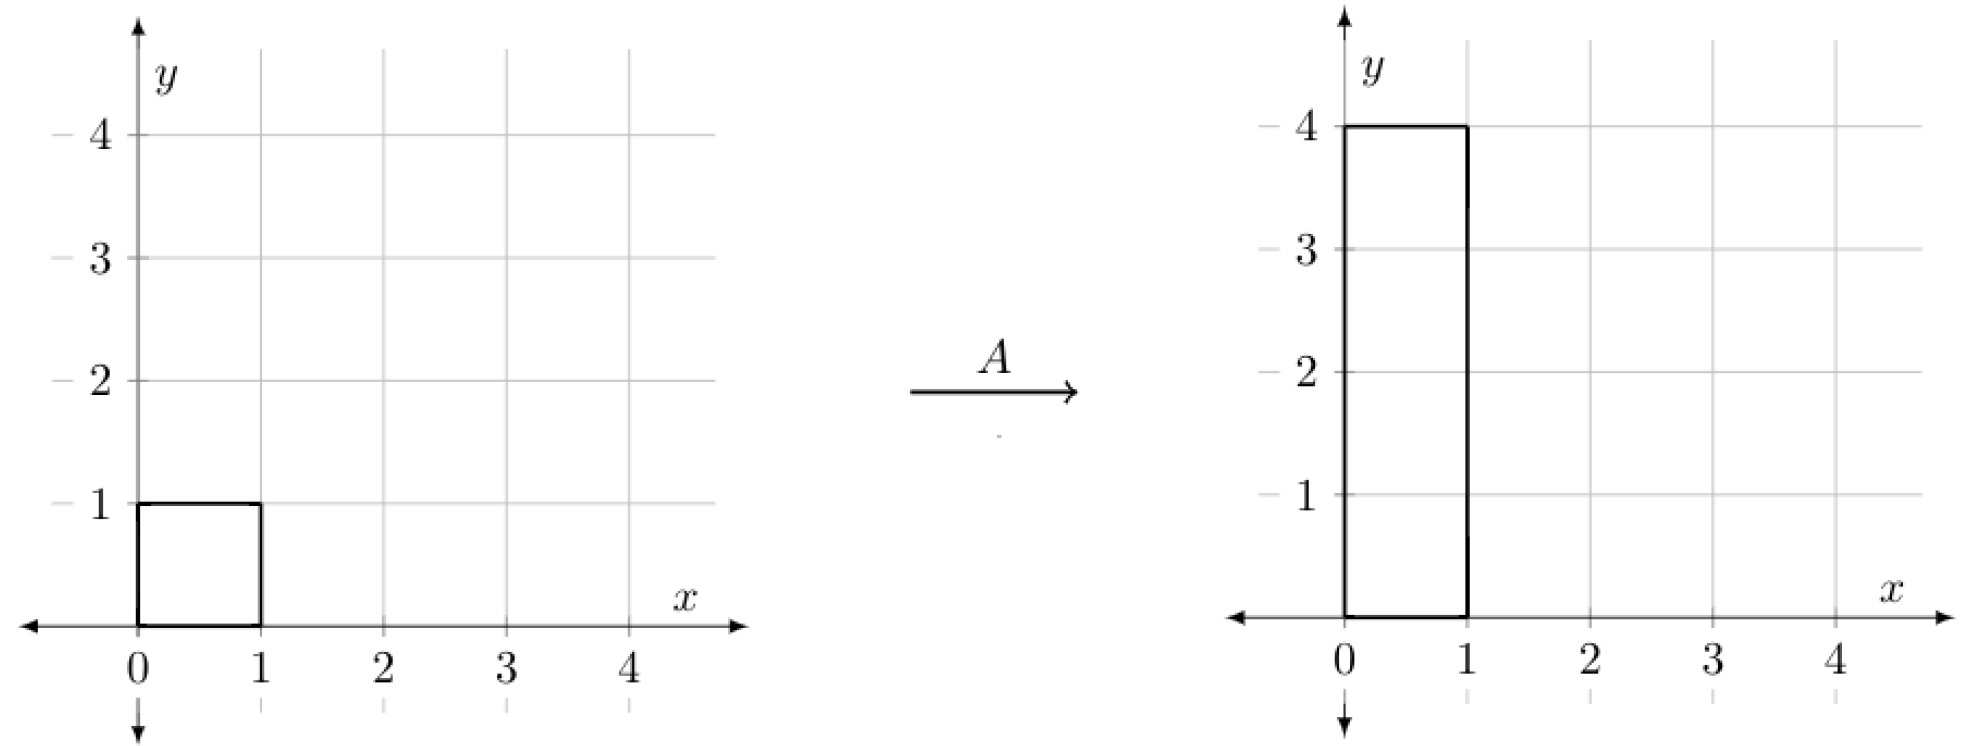
\includegraphics[scale=.5]{TransformationA.jpg}
\end{center}
Donc : la multiplication par une matrice diagonale est facile à comprendre.

	\item Qu'en est-il de la multiplication par $B = \scriptsize\mat{3&-1\\-2&2}$ ?  En l'appliquant
au m\^eme carré unitaire dont les sommets sont $(0,0)$, $(0,1)$, $(1,0)$, $(1,1)$, on obtient le parallélogramme dont les sommets sont :
$$
(0,0), (-1,2), (3,-2), (2,0)\,.
$$
\begin{center}
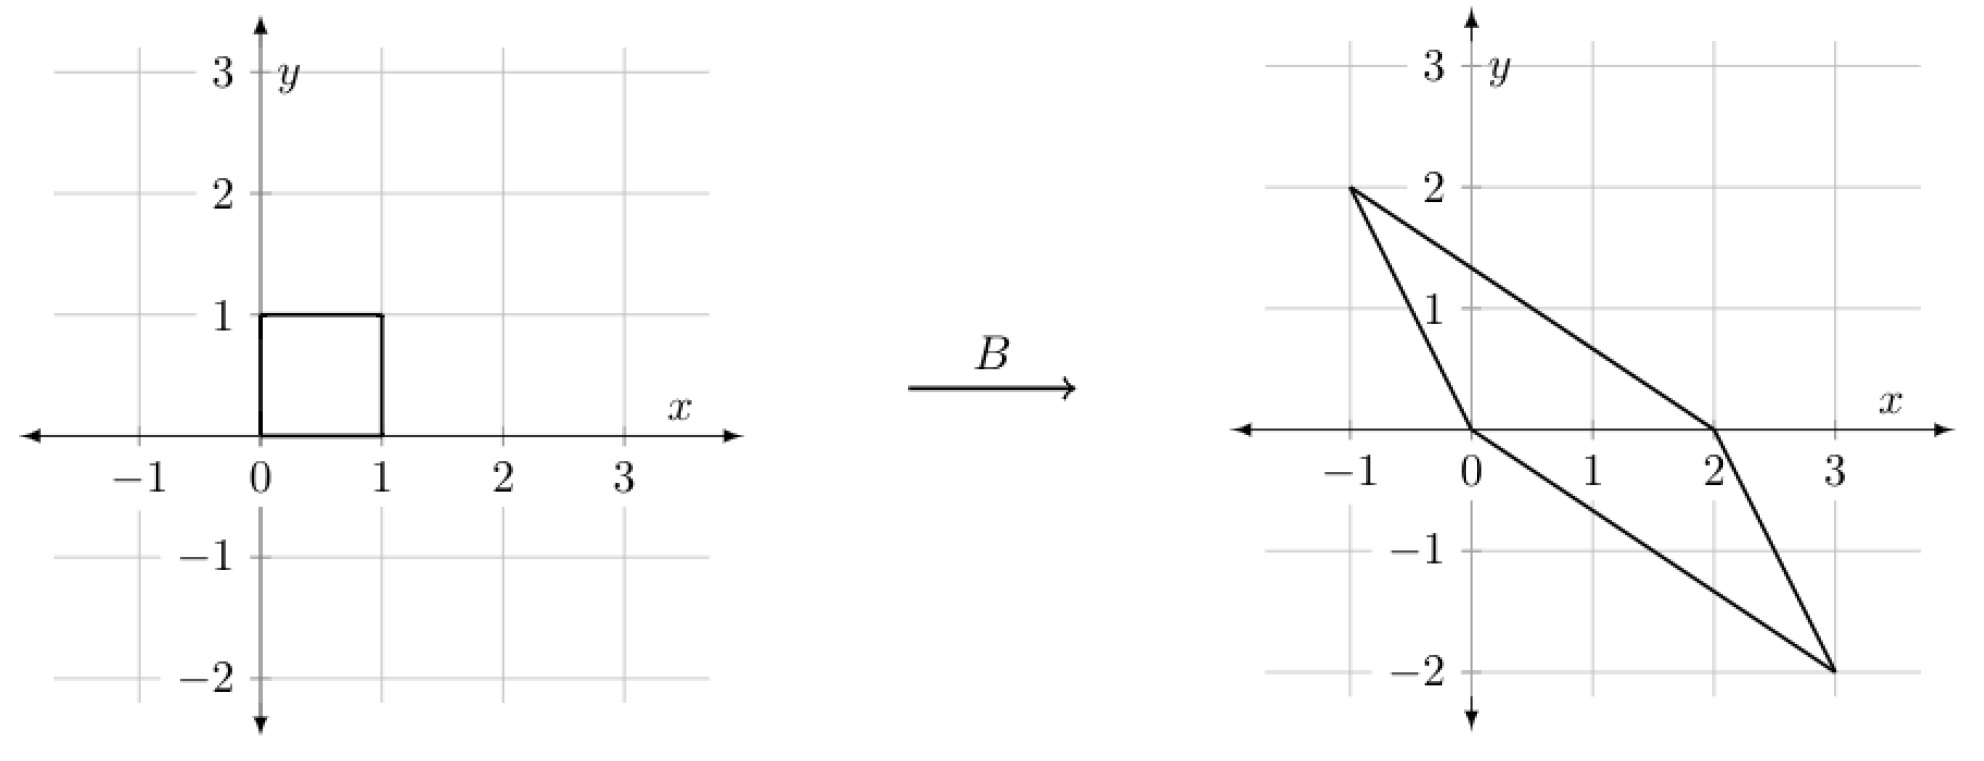
\includegraphics[scale=.5]{TransformationB1.jpg}
\end{center}
\end{enumerate}
Pourquoi y a-t-il une telle différence ?  
Le secret réside en fait dans les vecteurs propres. 
\begin{enumerate}[(1')]
	\item La matrice $A$ admet deux valeurs propres distinctes : $\lambda = 1$, à laquelle on peut associer le vecteur propre $(1,0)$, et $\lambda =4$, à laquelle on peut associer le vecteur propre $(0,1)$. Les espaces propres correspondent en fait aux axes canoniques : l'axe des $x$ et l'axe des $y$. C'est pour cela que la multiplication par $A$ transforme de manière aussi élégante le carré unitaire : parce que le carré unitaire a chacun de ses côtés parallèle à l'un des axes $x$ ou $y$, donc parallèle aux espaces propres.
	\item Faisons pareil pour $B$ : trouvons les axes avec lesquels il faut que les segments du dessin de départ soient parallèles pour mieux comprendre la transformation induite par $B$. La matrice $B$ admet deux valeurs propres distinctes : $\lambda = 1$, à laquelle on peut associer le vecteur propre $(1,2)$, et $\lambda =4$, à laquelle on peut associer le vecteur propre $(-1,1)$.
Considérons le parallélogramme dont les sommets sont ces deux vecteurs propres, l'origine, et le 4e sommet $(0,3)$:
$$
(0,0), (1,2), (-1,1), (0,3)\,.
$$
Alors, après multiplication par $B$, on obtient le parallélogramme :
$$
(0,0), (1,2), (-4,4), (-3, 6)\,.
$$
C'est le même parallélogramme, mais «~étiré~» 
d'un facteur de $4$ dans la direction $(-1,1)$. 
\begin{center}
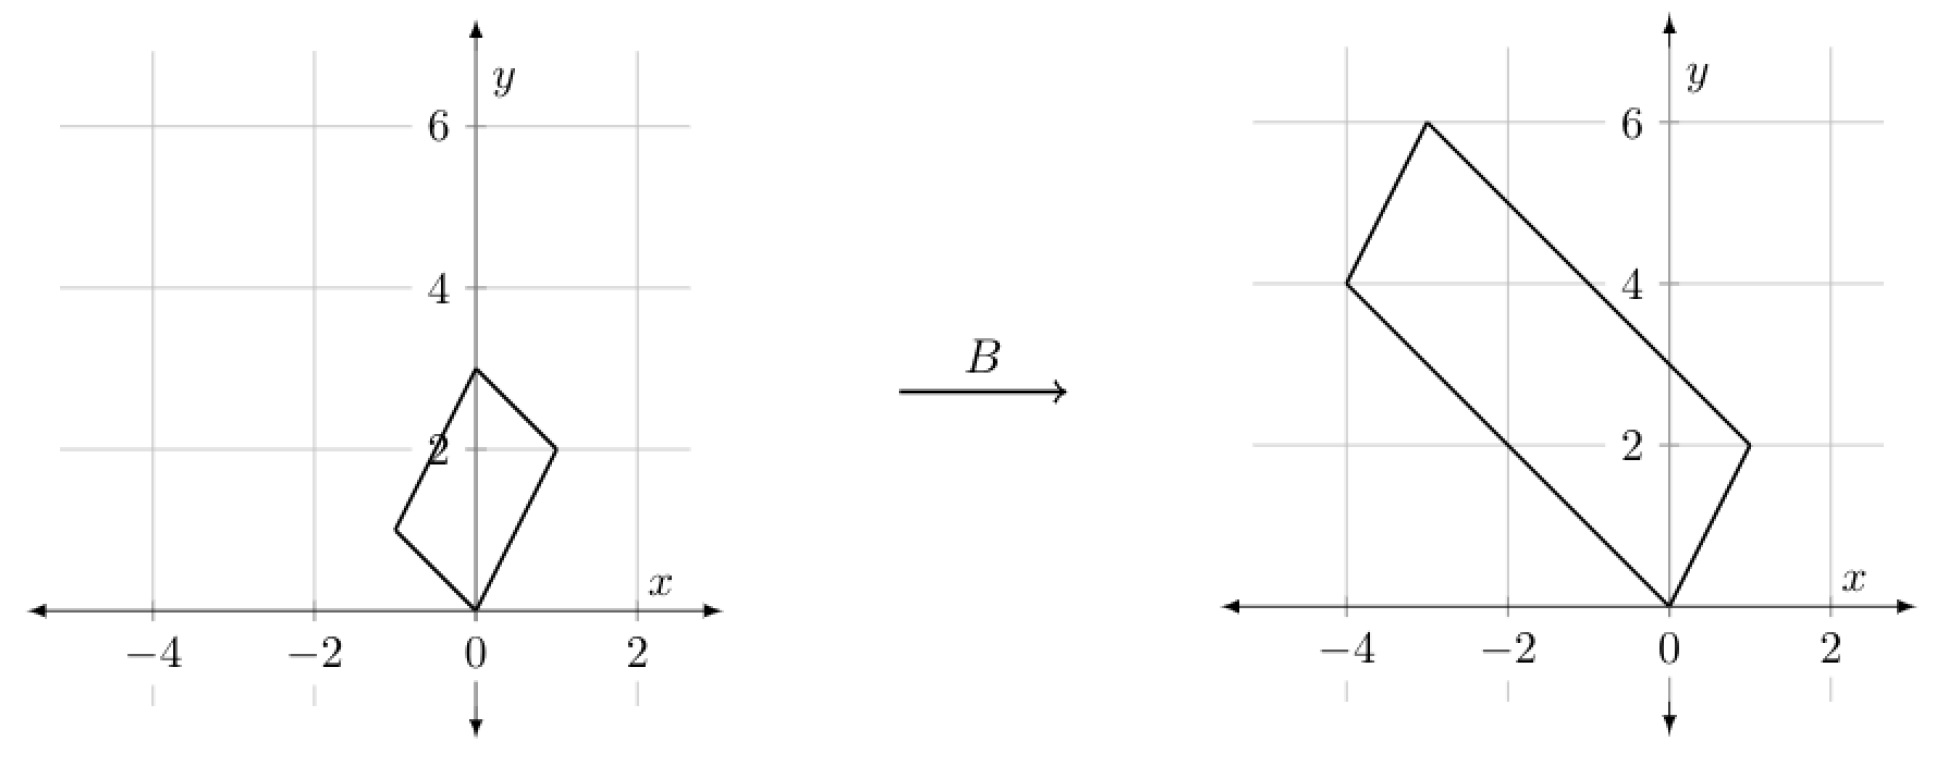
\includegraphics[scale=.5]{TransformationB2.jpg}
\end{center}
En fait, on voit alors que la matrice $B$ agit de la même manière que la matrice $A$, mais avec un angle différent ! Dans les deux cas, un axe est laissé intact, et l'autre est «~étiré~» d'un facteur $4$.
Par la même occasion, on comprend mieux aussi ce qui arrive à notre brave carr\'e unitaire dans le 2e schéma : il
a été étiré et déformé le long de deux droites différentes des axes $x$ et $y$, c'est pour cela qu'on obtenait un parallélogramme.
\end{enumerate}
Moralit\'e : les vecteurs propres sont le secret pour comprendre
la géométrie de la multiplication par une matrice.
\end{myexample}

Le fait de considérer une matrice $A$ de cette manière comme une transformation --- plus précisément comme une \stress{transformation linéaire} --- est un principe fondamental, avec de multiples applications notamment pour les systèmes dynamiques discrets et les processus de Markov\footnote{Recherchez sur le web  \og Chaînes de Markov\ \fg.} en probabilité.


Dans le prochain chapitre, ce que nous voulons faire, c'est explorer cette idée de transformations linéaires plus en détail
et revenir sur l'image qui illustre le lien entre le noyau $\ker(A)$ et l'espace image $\im(A)$ via une \emph{transformation} de
$\R^n$ dans $\R^m$ (la transformation étant : la multiplication par $A$, qui a $\xx\in\R^n$ associe $A\xx\in\R^m$).




\section*{Exercices}
\addcontentsline{toc}{section}{Exercices}


\medskip {\bf Remarques:} 
\begin{enumerate}
\item Une question marquée d'un astérisque $ ^\ast$ (ou deux) indique une question de niveau bonus.
 \item Vous devez justifier toutes vos réponses.
\end{enumerate}
\bigskip


\begin{prob} \label{prob23.1} 
\begin{enumerate}[a)]
\item Pour chacune des matrices $A$ de l'Exercice \ref{prob22.1}, si possible, trouvez une matrice inversible $P$ et une matrice diagonale $D$ telles que $P^{-1}AP =D$. Si ce n'est pas possible, expliquer pourquoi. (Les solutions aux questions b), d), f) et h) sont disponibles à la fin de l'ouvrage). 

\item Utilisez le fait que la matrice $A=\scriptsize\bmatrix 
1&0&1\\0&1&0\\1&1&1 \endbmatrix $ est diagonalisable pour calculer $A^{10^{1000}}$ avant que le soleil ne devienne une géante \'etoile rouge et n'engloutisse (éventuellement) la Terre... \footnote{Selon les estimations, vous avez donc entre 5 et 6 milliards d'années, mais cela ne devrait pas vous prendre plus de 5 minutes !\!!} 

\end{enumerate}

 

\end{prob} \begin{prob} \label{prob23.2}  Pour chacun des énoncés suivants, indiquez s'il est (toujours) vrai ou s'il est (possiblement) faux.    
\begin{enumerate}[$\bullet$]
\item Si vous dites que l'\'enonc\'e peut être faux, donnez un contre-exemple.   
\item Si vous dites que l'\'enonc\'e est vrai, donnez une explication claire - en citant un théorème ou en donnant une {\it preuve valide dans tous les cas}. 
\end{enumerate}
\smallskip

\begin{enumerate}[a)]
\item Si $\lambda=3$ est valeur propre d'une matrice $A$ de taille $n \times n$, alors il devrait exister un vecteur non-nul $\vv \in \R^n$ tel que $A\vv=3\vv$.
\medskip
 
\item\sov~La matrice $\bmatrix 0&-1\\1&0\endbmatrix$ n'admet pas de valeurs propres r\'eelles.
\medskip
 
\item La matrice $\bmatrix -1&1\\0&-1\endbmatrix$ est
diagonalisable.
\medskip
 
\item\sov~Si $0$ est valeur propre d'une matrice $A$ de taille $n \times n$, alors $A$ n'est pas inversible.
\medskip
 
\item Si une matrice $A$ de taille $n \times n$ n'est
pas inversible, alors $0$ est une valeur propre de $A$.
\medskip
 
\item\sov~Toute matrice inversible est diagonalisable.
\medskip
 
\item Toute matrice diagonalisable est inversible.
\medskip
 
\item\sov~Si une matrice de taille $n \times n$ admet $n$ valeurs propres distinctes, alors cette matrice est diagonalisable. 
\medskip
 
\item Si une matrice de taille $n \times n$ est diagonalisable, alors elle admet nécessairement $n$ valeurs propres distinctes. 
\medskip
 
\item\sov\footnote{ Indication : utilisez le fait que nous savons que $\det(A-\lam I_n)=(-1)^n(\lam-\lam_1)(\lam-\lam_2)\dots(\lam-\lam_n) $.} Si une matrice  $A$ de taille $n \times n$ admet des valeurs propres $\lam_1, \dots ,\lam_n$, alors $$\det (A)=\lam_1 \dots\lam_n\,.$$
 
\item$^{\ast}$\footnote{ Indication : puisque $A$ est symétrique, rappelez-vous que $A\vv\cdot \ww=\vv\cdot A\ww$ (voir l'Exercice \ref{prob14.4}). Simplifiez maintenant les deux côtés en utilisant le fait que $\vv$ et $\ww$ sont des vecteurs propres et regardez ce que vous obtenez.} Si $\vv$ et $\ww$ sont des vecteurs propres d'une matrice symétrique $A$ (c'est-à-dire une matrice $A$ qui vérifie $A=A^T$) et que $\vv$ et $\ww$ correspondent à des valeurs propres différentes, alors $$\vv \cdot \ww=0\,.$$  
\medskip
\end{enumerate}
\end{prob} 
\begin{prob} \label{prob23.3}\sov~Soit la matrice $A=\bmatrix
0&1&1\\ 1&0&1\\ 1&1&0 \endbmatrix$. 

\begin{enumerate}[a)]

\item Calculez $\det(A-\lam I_3)$ et montrez que les valeurs propres de
$A$ sont $\lambda = 2$ et $\lambda = -1$.

\item\sov~ Trouvez une base de $E_2 =\set{x\in \R^3 \st Ax= 2x}$.
\item\sov~ Trouvez une base de $E_{-1} =\set{x\in \R^3 \st Ax=-x}$. 
 
\item\sov~ Trouvez une matrice inversible 
$P$ telle que $P^{-1}AP=D$ soit diagonale, et donnez l'expression de cette matrice diagonale $D$. Expliquez pourquoi
la matrice $P$ que vous avez choisie est inversible.
\item\sov~ Trouvez une autre matrice inversible
$Q \not=P$ telle que $Q^{-1}AQ=\tilde D$ soit aussi diagonale, et donnez aussi l'expression de cette matrice diagonale $\tilde D$.
\end{enumerate}
  


\end{prob} 
\begin{prob} \label{prob23.4} $^{\ast}$\footnote{Cet exercice est une version simplifiée des équations du mouvement, en Mécanique, de deux masses reliées par un ressort. Cherchez sur internet le terme \og mode normal\ \fg\ pour voir un exemple. } Considérons le système d'équations différentielles suivant du second ordre en les deux fonctions $f$ et $g$ :

$$\begin{matrix} 
\ddot f=-2 f +g\,,  \\
\ddot g=f-2g\,.\\
 \end{matrix} $$
 (Ici, les notations $\ddot f$ et $\ddot g$ signifient respectivement $\frac{d^2 f}{dt^2}$ et $\frac{d^2 g}{dt^2}$.)
Ce système peut également être écrit sous forme matricielle comme suit: 
$$\bmatrix \ddot f \,\\ \ddot g
 \endbmatrix =\bmatrix -2 & 1 \\
 1 & -2 \endbmatrix \bmatrix  f \,\\   g
 \endbmatrix\,.$$ 

\begin{enumerate}[a)]
	\item Soit $A=\scriptsize\bmatrix -2 & 1 \\
 1 & -2 \endbmatrix $. Diagonaliser $A$ pour écrire $A=PDP^{-1}$, pour une certaine matrice inversible $P$ et une certaine matrice diagonale $D=\scriptsize\bmatrix \lam_1 & 0 \\
 0 & \lam_2 \endbmatrix $. 
 	\item Définissez maintenant deux nouvelles fonctions $h$ et $k$ par:
	$$\bmatrix h \,\\ k
 \endbmatrix = P^{-1} \bmatrix  f \,\\   g
 \endbmatrix\,.$$ 
 Montrez les équivalences de systèmes suivantes :
 $$\bmatrix \ddot f \,\\ \ddot g
 \endbmatrix =\bmatrix -2 & 1 \\
 1 & -2 \endbmatrix \bmatrix  f \,\\   g
 \endbmatrix
        \quad\Longleftrightarrow\quad
 \bmatrix \ddot h\,\\ \ddot k
 \endbmatrix =\bmatrix \lam_1 & 0 \\
 0 & \lam_2 \endbmatrix\bmatrix  h \,\\   k
 \endbmatrix
       \quad\Longleftrightarrow\quad
 \begin{matrix} 
\ddot h=\lam_1 \,h  \\
\ddot k=\lam_2 \,k\,.\\
 \end{matrix} $$ 

  	\item Vous constaterez que $\lam_1$ et $\lam_2$ sont tous deux négatifs, et donc les solutions de ces deux équations différentielles (linéaires) du second ordre sont les suivantes : 
	$$h(t)=a \sin( \sqrt{|\lam_1|}\,t) + b \cos( \sqrt{|\lam_1|}\,t)\,,$$ 
	$$k(t)=c \sin( \sqrt{|\lam_2|}\,t) + c \cos( \sqrt{|\lam_2}|\,t)\,,$$ 
	o\`u $a,b,c,d$ sont des constantes réelles.
  Utilisez ceci pour trouver $f$ et $g$, puis trouver les valeurs des constantes $a,b,c, d$ en fonction de ce que l'on appelle les {\it \og conditions initiales\ \fg\ $f(0), \dot f(0), g(0), \dot g(0)$}.

\end{enumerate}
 


\end{prob}




%%----------------------------------------------------------------------------------------
%%	PART VI: Linear Transformations
%%----------------------------------------------------------------------------------------

\chapterimage{Pinery.jpg} % Chapter heading image
%%Pinery20070816.jpg

\renewcommand{\partintrotext}{En mathématiques, quand on étudie un domaine, il est aussi important d'étudier les objets considérés --- les \emph{espaces vectoriels} dans notre cas --- que de comprendre les relations entre ces objets --- les \stress{transformations linéaires} dans notre cas. Ces relations entre les objets doivent être «~compatibles~» avec la structure des objets ; on aura donc quelques contraintes pour définir les transformation linéaires.  Notez que nous avons déjà vu et utilisé plusieurs de transformations linéaires : par exemple la multiplication par une matrice $A$, ou encore la projection sur un sous-espace.}

\part{Transformations linéaires}


\chapter{Transformations linéaires}
\label{chapter:Fr_29-lineartransformations}


La dernière fois, nous avons vu l'interprétation géométrique de la \og multiplication
par $A$\ \fg: c'est une transformation de $\R^n$ dans $\R^m$ (si $A$ est une matrice de taille $m\times n$), et elle est un peu spéciale : elle transforme des carrés en parallélogrammes (contrairement 
à tout ce que votre imagination pourrait produire!).

Les propriétés clés qui font que cela fonctionne sont:
\begin{itemize}
\item $A\zero = \zero$;
\item $A(\uu + \vv) = A\uu + A\vv$ pour tout $\uu,\vv \in \R^n$;
\item $A(r\uu) = r(A\uu)$ pour tout $\uu\in\R^n$, $r\in\R$.
\end{itemize}
Ces propriétés impliquent que les quatre sommets suivants 
d'un parallélogramme :
$$
\zero, \uu, \vv, \uu+\vv
$$
 sont
envoyés aux quatre points suivants :
$$
\zero, A\uu, A\vv, A\uu + A\vv\,,
$$
lesquels définissent encore une fois les sommets d'un parallélogramme (bien que ce parallélogramme puisse \^etre
dégénéré (\textit{i.e.} être aplati sur un segment) dans des cas défavorables, dès lors que $A\uu$ et $A\vv$ sont linéairement dépendants). Notez qu'une droite est envoyée sur une droite :
la droite $\{r\uu\,|\,r\in\R\}$ est envoyée sur la droite
$\{r(A\uu) \,|\, r\in\R\}$ (il se peut néanmoins que ce soit seulement un point et pas une droite si $A\uu=\zero$). Etc...


\begin{definition}
Soient $U$ et $V$ des espaces vectoriels.  Une \defn{transformation linéaire} $T$
est une transformation de $U$ en $V$ satisfaisant 
\begin{enumerate}[(1)]
\item pour tout $\uu,\vv\in U$, $T(\uu+\vv) = T(\uu)+T(\vv)$;
\item et pour tout $\uu \in U$, $r\in\R$, $T(r\uu) = rT(\uu)$.
\end{enumerate}
\end{definition}

Nous utilisons ici le terme \stress{transformation} ;
nous aurions pu aussi utiliser le terme \stress{fonction}, mais ce mot est souvent plutôt réservé aux applications dont l'image est $\R$. Enfin bref, quoi qu'il en soit, quelle que soit la terminologie utilisée,
l'essentiel est de comprendre que $T$ est une boîte noire, c'est une formule ou une règle qui
prend un vecteur $\uu\in U$ en entrée et qui produit un vecteur $\vv\in V$
en sortie, et ce vecteur $\vv$ est totalement déterminé par $T$ (ce vecteur n'est pas aléatoirement choisi). Dans la définition, pour que la transformation soit \emph{linéaire}, nous précisons en plus que nous voulons que $T$ transforme les sommes en sommes, et les multiples scalaires en... multiples scalaires ! Pas si surprenant non ? En d'autres termes, nous voulons simplement qu'une transformation linéaire \emph{préserve la linéarité} !

En particulier : la multiplication par une matrice carrée $A$ est bien une transformation linéaire, puisqu'elle satisfait tous les points de cette définitions.\\

Nous devons maintenant nous demander : quels autres types de transformations linéaires
connaissons-nous déjà ?



\section{Exemples de transformations linéaires}

\begin{myexample}\label{ex:multmatlintrans}
 Soit $A$ une matrice de $m\times n$.  On définit la transformation
$$T_A \colon \R^n \to \R^m
$$
par $T_A(\uu) = A\uu$.  Vérifions que $T_A$ est bien une transformation linéaire.
\begin{enumerate}
\item Pour tout $\uu,\vv \in \R^n$, nous avons bien $T_A(\uu+\vv) = T_A(\uu) +T_A(\vv)$ puisque :
$$
T_A(\uu+\vv) = A(\uu + \vv) = A\uu + A\vv =  T_A(\uu) +T_A(\vv)\,.
$$
\item Pour tout $\uu \in \R^n$, $r\in \R$, nous avons également $T_A(r\uu) = rT_A(\uu)$ puisque :
$$
T_A(r\uu) = A(r\uu) = r(A\uu) = rT_A(\uu)\,.
$$
\end{enumerate}
Il s'agit donc bien d'une transformation linéaire, pour n'importe quelle matrice $A$ à coefficients réels de n'importe quelle taille $m\times n$.
\end{myexample}

\begin{myexample} Considérons la projection sur le plan $W$ défini par
$$
W = \{ (x,y,z) \mid x-z = 0\}\,.
$$
Est-ce que $\proj_W$ est une transformation linéaire ? Trouvons d'abord une formule pour cette projection.  Le moyen le plus simple
est sans doute de remarquer que l'orthogonal de $W$ est $W^\perp = \spn\{(1,0,-1)\}$. Donc pour $\uu = (u_1,u_2,u_3)\in \R^3$, on a
$$
\proj_{W^\perp}(\uu) = \frac{\uu \cdot (1,0,-1)}{(1,0,-1)\cdot (1,0,-1)} \mat{1\\0\\-1}
= \frac{u_1-u_3}{2}\mat{1\\0\\-1}
$$
et alors
$$
\proj_W(\uu) = \uu - \proj_{W^\perp}(\uu) =\mat{u_1\\u_2\\u_3} - \frac{u_1-u_3}{2}\mat{1\\0\\-1} = \frac12\mat{u_1+u_3\\ 2u_2 \\ u_1+u_3}.
$$

Est-ce donc une transformation linéaire?  Vérifions les deux propriétés de
linéarité (avec $T = \proj_W$).
\begin{enumerate}
\item Est-ce que $\proj_W(\uu + \vv) = \proj_W(\uu) + \proj_W(\vv)$? Soient $\uu = (u_1, u_2, u_3)$ et $\vv = (v_1, v_2, v_3)$. Alors
\begin{align*}
\proj_W(\uu + \vv) &= \proj_U(u_1+v_1,u_2+v_2,u_3+v_3) \\
&= \frac12\mat{ (u_1+v_1) + (u_3+v_3)\\ 2(u_2+v_2)\\  (u_1+v_1) + (u_3+v_3)}\\
&= \frac12\left( \mat{u_1+u_3\\2u_2\\u_1+u_3} + \mat{v_1+v_3\\2v_2\\v_1+v_3}\right) \\
&= \frac12\mat{u_1+u_3\\2u_2\\u_1+u_3} + \frac12\mat{v_1+v_3\\2v_2\\v_1+v_3}\\
&= \proj_W(\uu) + \proj_W(\vv)
\end{align*}
comme requis.
\item Est-ce que $\proj_W(r\uu) = r\proj_W(\uu)$?  Soient $r\in \R$ et $\uu\in\R^n$.
Alors
\begin{align*}
\proj_W(r\uu) &= \proj_W(ru_1,ru_3,ru_3)\\
&= \frac12\mat{ru_1+ru_3\\ 2ru_2 \\ ru_1+ru_3}\\
&= r\left(\frac12\mat{u_1+u_3\\ 2u_2 \\ u_1+u_3}\right)\\
&= r\proj_W(\uu)
\end{align*}
comme requis également.
\end{enumerate}
Donc les deux axiomes sont satisfaits et il s'agit bien d'une transformation linéaire !
\end{myexample}

\begin{myexample} Montrons que la transformation $T \colon \R^2 \to \R^2$ d\'efinie par
$$T(x,y) = (x+1, xy)$$ n'est PAS une transformation linéaire.

Il suffit de montrer qu'il existe une paire de vecteurs $\uu,\, \vv$ 
pour lesquels $T(\uu+\vv) \neq T(\uu)+T(\vv)$ ; OU de montrer qu'il existe
un vecteur $\uu$ et un scalaire $r$ pour lesquels $T(r\uu) \neq rT(\uu)$.
Montrons en fait un résultat plus fort dans ce cas-ci : ces deux axiomes échouent pour presque tous les vecteurs
et tous les scalaires !\!!

\begin{enumerate}
\item D'une part : $$T(\uu + \vv) = T(u_1+v_1,u_2+v_2) = (u_1+v_1+1, (u_1+v_1)(u_2+v_2))\,,$$
d'autre part :
$$
T(\uu) + T(\vv) = (u_1+1,u_1u_2) + (v_1+1, v_1v_2) = (u_1+v_1+2, u_1u_2+v_1v_2)\,.
$$
Mais les premières composantes $u_1+v_1+1$ et $u_1+v_1+2$ ne peuvent JAMAIS être égales... Donc on ne peut JAMAIS avoir $T(\uu+\vv) = T(\uu)+T(\vv)$. (D'ailleurs les secondes composantes ci-dessus ne sont égales que si les \og termes croisés\ \fg\ sont nuls.)

Par exemple, on a $T(1,0)=(2,0)$, $T(0,1)=(1,0)$ et $$T(1,1)=(2,1) \not=(2,0)+(1,0)=T(1,0) +T(0,1).$$

Nous pourrions nous arrêter là : nous avons trouvé un exemple qui montre que $T$ n'est pas linéaire. Mais montrons que $T$ ne satisfait pas non plus la deuxième condition.
\item D'un côté on a :
$$
T(r\uu) = T(ru_1,ru_2) = (ru_1+1, (ru_1)(ru_2)) = (ru_1+1, r^2u_1u_2)\,,
$$
mais d'un autre côté on a :
$$
rT(\uu) = r(u_1+1,u_1u_2) = (ru_1+r, ru_1u_2)\,.
$$
L\`a encore, la première composante est égale \`a la seconde seulement quand $r=1$, $r=0$ ou $u_1u_2=0$. 

Donc, par exemple, en prenant $\uu =(1,1)$ et $r=2$, on a : 
$$T(2(1,1))=T(2,2)=(3, 4)\not= 2(2,1)=2\, T(1,1)\,,$$
Donc le deuxième critère n'est pas non plus vérifié.
\end{enumerate}
Cette transformation n'est donc clairement pas linéaire.
\end{myexample}


\section{Construction et description d'une transformation linéaire}

Pour vérifier qu'une transformation est linéarité, on fait des étapes étrangement similaires au test du sous-espace.  Est-ce la même chose ?  NON : le
test du sous-espace concerne les ensembles, tandis que les transformations linéaires sont des applications
entre des espaces vectoriels (ou des sous-espaces).

Le terme \og transformation linéaire\ \fg\ vient (en partie) du fait que
l'image par $T$ d'une droite passant par l'origine est de nouveau une droite passant par l'origine (ou simplement le singleton $\set{\zero}$).

De plus, en prenant $r=0$, la deuxième propriété de la définition nous dit que toute transformation linéaire vérifie l'égalité:
$$T(\zero) = \zero\,.$$

Mais en fait, les deux propriétés de la définition impliquent bien plus de choses : elles disent que les combinaisons linéaires sont envoyées sur des combinaisons linéaires, au sens suivant :

\begin{theorem}[Une transformation linéaire est déterminée par son image d'une base]\label{Thm:LTbasis} \index{determination des transformations lineaires a partir d'une base@détermination des transformations linéaires \`a partir d'une base}
~
\begin{enumerate}
\item Soit $T \colon U \to V$ une transformation linéaire et soit
$\{ \uu_1, \cdots, \uu_n\}$ une base de $U$.  Alors $T$
est complètement et uniquement déterminée par son image de la base : 
$$T(\uu_1), \cdots,
T(\uu_n)\,.$$
En d'autres termes, si l'on connait seulement les $n$ valeurs de $T$ aux vecteurs de la base $\{ \uu_1, \cdots, \uu_n\}$, alors on connait toutes les valeurs de $T$ partout dans $U$ (donc pas seulement dans la base) ; il n'y qu'une seule transformation linéaire qui vérifie cela.
\item Soit $\{ \uu_1, \cdots, \uu_n\}$ une base de $U$
et soit $\{ \vv_1, \cdots, \vv_n\}$ un  {\it ensemble quelconque} de $n$ vecteurs de $V$ (ils ne forment pas forcément une base de $V$, ils peuvent même
éventuellement être lin\'eairement dépendants ou même tous nuls par exemple si l'on veut !).  Alors il existe une \emph{unique} transformation 
linéaire $T$ qui satisfait $$T(\uu_i)=\vv_i$$ pour tout $i$.
\end{enumerate}
\end{theorem}

\begin{proof}
\begin{enumerate}
\item Ce que nous voulons dire par \og complètement et uniquement déterminée\ \fg, c'est que nous pouvons
connaître la valeur de $T(\uu)$ pour n'importe quel $\uu$ de $U$ sans pour autant connaître une formule pour $T$, seulement en fixant les vecteurs $T(\uu_1),\cdots,T(\uu_n)$. C'est fort ! Montrons le résultat. Soit $\uu \in U$ un vecteur arbitraire.  Puisque
$\{ \uu_1, \cdots, \uu_n\}$ est une base pour $U$, nous pouvons
écrire
$$\uu = a_1\uu_1+\cdots+a_n\uu_n$$
pour certains scalaires $a_1,\dots,a_n\in\R$.
Alors, en utilisant les deux propriétés d'une transformation linéaire, on en déduit l'expression de $T(\uu)$ :
$$
T(\uu) = T(a_1\uu_1+\cdots+a_n\uu_n) = a_1T(\uu_1) + \cdots + a_nT(\uu_n)\,.
$$
D'où $T$ est complètement et uniquement déterminée par ces $n$ vecteurs de $V$.
\item Pour montrer l'existence, nous devons trouver la formule d'une transformation $T$ qui envoie $\uu_i$ à $\vv_i$.
Utilisons l'idée ci-dessus : pour tout $\uu \in U$, \'ecrivons $\uu = a_1\uu_1+\cdots+a_n\uu_n$.  On d\'efinit alors la transformation $T$ par
$$
T(\uu) = a_1\vv_1 + \cdots + a_n\vv_n\,,
$$
et on obtient bien une transformation de $U$ à $V$ et on vérifie qu'elle est bien linéaire (essayez-le !). En ce qui concerne l'unicité, elle découle du point précédent.
\end{enumerate}
\end{proof}

Ce théorème est très fort !\!!  Faisons une analogie avec de que nous avons vu dans les chapitres précédents : on sait que prouver
l'existence d'une base pour tout espace vectoriel de dimension finie est très important, ça simplifie les choses
et ça nous permet de voir tout espace vectoriel de dimension $n$ un peu comme $\R^n$. De même ici, le théorème nous dit que toute
transformation linéaire n'est en fait qu'une multiplication matricielle, pour une matrice bien choisie, dès lors que les espaces vectoriels sont de dimension finie ! Wow, impressionnant n'est-ce pas ?\!!

\begin{theorem}[La matrice standard d'une transformation linéaire]\index{matrice standard d'une transformation linéaire}\label{thm:standt_mat}
Soit $T \colon \R^n \to \R^m$ une transformation linéaire.  Alors
il existe une matrice $A$ de taille $m\times n$ telle que
$$
T(\xx) = A\xx
$$
pour tout $\xx \in \R^n$.  Plus précisément, si $\{\ee_1, \cdots, \ee_n\}$
est la base standard de $\R^n$, alors on sait même que l'expression de la matrice $A$ est
(en écriture par blocs de colonnes) :
$$
A = \left[ T(\ee_1) \;  T(\ee_2)\; \cdots \;   T(\ee_n)\right].
$$
Cette matrice $A$ ainsi définie est appelée la \defn{matrice standard} de $T$.
 \end{theorem}

\begin{myexample}
Comme précédemment, considérons la projection $T = \proj_W$ sur le plan $W = \{(x,y,z)\mid x-z=0\}$. Nous avons vu que $T(u_1, u_2,u_3) = \frac12(u_1+u_3,\,2u_2,\,u_1+u_3)$.

On construit la matrice comme dans le théorème : on calcule ses colonnes  $T(1,0,0) = (\frac12,0,\frac12)$, $T(0,1,0) = (0,1,0)$, $T(0,0,1) = (\frac12,0,\frac12)$, ce qui donne :
$$
A = \mat{\frac12 & 0 & \frac12\\ 0 & 1 & 0\\ \frac12 & 0 & \frac12}\,.
$$
On vérifie facilement qu'on a bien l'égalité voulue entre $A$ et $T$ :
$$
A\uu =  \mat{\frac12 & 0 & \frac12\\ 0 & 1 & 0\\ \frac12 & 0 & \frac12}\mat{u_1\\u_2\\u_3} = \frac12\mat{u_1+u_3\\2u_2\\u_1+u_3} = T(\uu)\,.
$$
\end{myexample}

\begin{proof}
Pour voir pourquoi ce théorème fonctionne, rappelez-vous que si vous avez un vecteur
$$\uu = \mat{u_1 \\ u_2 \\ \vdots \\ u_n},
$$
alors ce vecteur s'écrit aussi en fait comme suit:  
$$
\uu = u_1\ee_1 + \cdots + u_n\ee_n.
$$
Donc $T(\uu)$, par le Th\'eor\`eme~\ref{Thm:LTbasis}, 
est uniquement et complètement déterminée par la relation
$$
T(\uu) = u_1 T(\ee_1) + \cdots + u_nT(\ee_n).
$$
Or, prendre un combinaison linéaire revient à faire une multiplication matricielle. Donc en fait, nous avons:
$$
T(\uu) = \left[ T(\ee_1) \;  T(\ee_2)\; \cdots \;   T(\ee_n)\right]
\mat{u_1 \\ u_2 \\ \vdots \\ u_n} = A\uu\,.
$$
D'où le résultat !
\end{proof}


\section{Noyau et image d'une transformation linéaire}

Cette nouvelle interprétation de la projection comme une transformation linéaire
nous donne des idées plus géométriques sur ce que l'opération de projection
fait réellement.  Par exemple, la projection sur $W$ annule (\textit{i.e.} elle renvoie
$\zero$ pour) tout vecteur de $W^\perp$.  Par contre, elle «~couvre complètement $W$~»
avec son image, dans le sens où chaque vecteur de $W$ est l'image d'au moins un élément de $\R^n$ par la projection.

Pour rendre cela plus clair, nous avons besoin de quelques définitions.

\begin{definition}
Soit $T \colon U \to V$ une transformation linéaire.  Alors
\begin{itemize}
\item Le \defn{noyau} de $T$, noté $\ker(T)$, est l'ensemble de tous les vecteurs de $U$ dont l'image par $T$ est $\zero$;
c'est-à-dire,
$$
\ker(T) = \{ \uu \in U \mid T(\uu) = \zero\}\,.
$$
\item L'\defn{image} de $T$, notée $\im(T)$, est l'ensemble de tous les
vecteurs de $V$ qui sont égaux à $T(\uu)$ pour un certain $\uu \in U$;
c'est-à-dire,
$$
\im(T) = \{ \vv \in V \mid \vv = T(\uu) \; \textrm{pour un certain $\uu\in U$}\}\,.
$$
\end{itemize}
\end{definition}

Notez que $\ker(T)$ et $\im(T)$ sont tous deux des \emph{sous-ensembles} d'espaces vectoriels. Donc
un première question naturelle est : sont-ils des \emph{sous-espaces} ?  Réponse :  OUI,
et ce sont même des sous-espaces qu'on connait déjà !

\begin{theorem}[Noyau et image de la matrice standard]\index{noyau de $A$  vs noyau de $T$}\index{image vs noyau de $A$}
Soit $T \colon \R^n \to \R^m$ une transformation linéaire, et soit $A$ sa 
matrice standard.  Alors
$$
\ker(T) = \ker(A) \qquad \textrm{et} \qquad \im(T) = \im(A)\,.
$$
\end{theorem}

La première égalité est claire une fois que l'on se rappelle que $T(\uu) = A\uu$ ;
et pour la seconde, il faut retourner en arrière et chercher la définition originale de
$\im(A)$, mais ce n'est pas très dur non plus.

\section{Le Théorème du rang revisit\'e}

Notez que le théorème du rang\footnote{Certains aiment appeler ce théorème le {\it Théorème de la conservation de la dimension}, puisque la dimension du sous-espace envoyé à $\zero$ (le noyau) ajoutée à la dimension de l'image de $T$ (ce qui reste), est la même que la dimension de l'espace de départ ($n=\dim U$). Donc, \og la dimension totale est conservée\ \fg\ en ce sens.} peut \^etre reformul\'e, pour
une transformation linéaire $T \colon U \to V$, comme suit :
$$
\dim(\ker(T)) + \dim(\im(T)) = n,
$$
où $n = \dim(U)$. Ainsi, aucune information sur $T$ ne se perd.
Si par exemple $T$ envoie $U$ sur un sous-espace de $V$ de dimension
égale à $U$, alors le noyau doit être égal à $\{\zero\}$.
Par contre, si la dimension de l'image $\dim(\im(T))$ est strictement inférieure à la dimension de l'espace de départ $\dim (U)$, alors les dimensions manquantes sont allées autre part : on les retrouve dans le noyau de $T$. \\

Par exemple, revenons à la projection sur le plan $W$ que nous avons vu
plus tôt. Elle a un noyau de dimension 1, donn\'e par le sous-espace $W^\perp$,
et une image de dimension $2$, c'est tout le plan $W$. On a bien le Théorème du rang qui est vérifié dans ce cas: 
$$2+1=3 = \dim(\R^3)\,.$$


Réciproquement, comme on peut penser à $T$ comme à une matrice, une base de $\im(T)$ sera alors également une base de l'espace des colonne $\col(A)$, et vis-versa une base de $\col(A)$ sera alors également une base de $\im(T)$.

\section{Remarques sur la matrice projection}
Dans les chapitres précédents, lorsque nous avons calculé la projection sur le sous-espace $W$, une de nos méthodes était :
\begin{enumerate}[(1)]
\item créez une matrice $B$ telle que $\im(B) = W$;
\item r\'esoudre le système $(B^TB)\xx = B^T\bb$; 
\item et enfin en déduire que $\proj_W(\bb) = B\xx$.
\end{enumerate}
Résumons ceci différemment :  supposons que $B$ ait des colonnes linéairement indépendantes. Alors $B^TB$ est inversible.  (Ceci était un exercice.)
Alors on a
$$
\proj_W(\bb) = B(B^TB)^{-1}B^T\bb
$$
et donc la projection est donnée par la multiplication par la matrice
$$
 B(B^TB)^{-1}B^T.
$$
Par conséquent, on en déduit que cette derni\`ere matrice est nécessairement la \emph{matrice standard} de $T$!  Vous pouvez
v\'erifier cela pour l'exemple que nous avions vu.



\section*{Exercices}
\addcontentsline{toc}{section}{Exercices}


\medskip {\bf Remarques:} 
\begin{enumerate}
\item Les questions marquées d'un astérisque $ ^\ast$ (ou deux) indiquent des questions de niveau bonus.
 \item Vous devez justifier toutes vos réponses.
\end{enumerate}
\bigskip



 \begin{prob} \label{prob24.1}  Pour chacune des transformations suivantes, indiquez si elle est linéaire ou non.   
   \smallskip    
\begin{enumerate}[$\bullet$]
\item Si vous dites qu'elle ne l'est pas, donnez un contre-exemple.   
\item Si vous dites qu'elle l'est, donnez une explication claire - en citant un théorème ou en donnant une {\it preuve valide dans tous les cas}. 
\end{enumerate}
\medskip

\begin{enumerate}[a)]
\item  $T:\R^2 \to \R^3$ d\'efinie par $T(x,y)=(x, y, x+y)$.
\medskip
 
\item\sov~$T:\R^3 \to \R^2$ d\'efinie par $T(x,y,z)=(2 z+x, y)$.
\medskip
 
\item $T:\R^2 \to \R^2$ d\'efinie par $T(x,y)=(x, x y)$.
\medskip
 

\item\sov~$T:\R^2 \to \R^2$ d\'efinie par $T(\vv)=\bmatrix 0&-1\\ 1&0 \endbmatrix \vv$.
\medskip
 
\item $T:\R^3 \to \R^3$ d\'efinie par $T(\vv)= \vv\times (1,2,3)$, o\`u \og\  $\times$\ \fg\ d\'enote le produit vectoriel.
\medskip
 

\item\sov~$T:\R^3 \to \R^3$ d\'efinie par $T(\vv)= \proj_{(1,1,-1)}(\vv)$.
\medskip
 
\item $T:\R^3 \to \R^3$ d\'efinie par $T(\vv)= \vv-\proj_{(1,1,-1)}(\vv)$.
\medskip
 
\item\sov~$T:\R^3 \to \R^3$ d\'efinie par $T(\vv)= \proj_{\vv}(1,1,-1)$.
\medskip
 
\item $T:\R^3 \to \R^3$ d\'efinie par $T(\vv)= \big(\vv \cdot (1,1,-1)\big) (1,0,1)$.
\medskip
 
\item\sov~$T:\R^3 \to \R^3$ d\'efinie par $T(\vv)= 2 \vv$.
\medskip
 
\item $T:\R^3 \to \R^3$ d\'efinie par $T(\vv)= \proj_H(\vv)$, où $H$ est le plan passant par l'origine et de vecteur normal $(1,1,0)$.
\medskip
 
\item\sov~$T:\R^3 \to \R^2$ d\'efinie par $T(\vv)= A\vv$, où $A=\bmatrix 1&0&1\\ 1&2&3\endbmatrix$.
\medskip

\end{enumerate} 

\end{prob} \begin{prob} \label{prob24.2} Dans chacun des cas suivants, déterminez la matrice standard de $T$, puis utilisez-la pour trouver une base de $\ker( T)$ et une base de $\im( T)$. Enfin, vérifiez la conservation de la dimension (\textit{i.e.} le Théorème du rang). 

\medskip
\begin{enumerate}[a)]
\item $T:\R^2 \to \R^3$ d\'efinie par $T(x,y)=(x, y, x+y)$.
\medskip
 
\item\sov~$T:\R^3 \to \R^2$ d\'efinie par $T(x,y,z)=(2 z+x, y)$.
\medskip
 
\item $T:\R^3 \to \R^3$ d\'efinie par $T(\vv)= \vv\times (1,2,3)$, o\`u \og\  $\times$\ \fg\ d\'enote le produit vectoriel.
\medskip
 
\item\sov~$T:\R^3 \to \R^3$ d\'efinie par $T(\vv)= \proj_{(1,1,-1)}(\vv)$.
\medskip
 
\item $T:\R^3 \to \R^3$ d\'efinie par $T(\vv)= \vv-\proj_{(1,1,-1)}(\vv)$.
\medskip
 
\item\sov~$T:\R^3 \to \R^3$ d\'efinie par $T(\vv)= \proj_H(\vv)$, où $H$ est le plan passant par l'origine et de vecteur normal $(1,1,0)$.
\medskip
 
\end{enumerate}

\end{prob} \begin{prob} \label{prob24.3}  Pour chacun des énoncés suivants, indiquez s'il est (toujours) vrai ou s'il est (possiblement) faux.   
   \smallskip    
\begin{enumerate}[$\bullet$]
\item Si vous dites que l'\'enonc\'e peut être faux, donnez un contre-exemple.   
\item Si vous dites que l'\'enonc\'e est vrai, donnez une explication claire - en citant un théorème ou en donnant une {\it preuve valide dans tous les cas}. 
\end{enumerate}
\medskip
\begin{enumerate}[a)]
\item Si une transformation $T:\R^3 \to \R^2$ est lin\'eaire, alors $\ker(T) \not= \set{\zero}$.
\medskip
 
\item\sov~Si une transformation $T:\R^4 \to \R^2$ est lin\'eaire, alors $\dim \ker(T) \ge 2$.
\medskip
  
\item Si une transformation $T:\R^4 \to \R^5$ est lin\'eaire, alors $\dim \im(T) \le 4$.
\medskip
 
\item\sov~Si une transformation $T:\R^3 \to \R^2$ est lin\'eaire et que $\set{\vv_1,\vv_2} \subset \R^3$ est lin\'eairement ind\'ependant, alors $\set{T(\vv_1),T(\vv_2)} \subset \R^2$ est aussi lin\'eairement ind\'ependant.
\medskip
 
\item Si une transformation $T:\R^3 \to \R^2$ est lin\'eaire, que $\ker(T)=\set{\zero}$ et que $\set{\vv_1,\vv_2} \subset \R^3$  est lin\'eairement ind\'ependant, alors $\set{T(\vv_1),T(\vv_2)} \subset \R^2$ est aussi lin\'eairement ind\'ependant.
\medskip
 
\item\sov~Si une transformation $T:\R^3 \to \R^3$ est lin\'eaire et que $\ker(T)=\set{\zero}$, alors $\im(T)=\R^3$.
\medskip
 
\item Si une transformation $T:\R^2 \to \R^3$ est lin\'eaire et que $\ker(T)=\set{\zero}$, alors $\im(T)=\R^3$.

\end{enumerate}

\end{prob} \begin{prob} \label{prob24.4}$^\ast$ Pour chacune des transformations suivantes, indiquez si elle est linéaire ou non.   
   \smallskip    
\begin{enumerate}[$\bullet$]
\item Si vous dites qu'elle ne l'est pas, donnez un contre-exemple.   
\item Si vous dites qu'elle l'est, donnez une explication claire - en citant un théorème ou en donnant une {\it preuve valide dans tous les cas}. 
\end{enumerate}
 \medskip
\begin{enumerate}[a)]
\item $T: \PP \to \PP$ d\'efinie par $T(p)=p'$, où $p'$ désigne la dérivée du polynôme $p$.
\medskip
 
\item\sov~$T: \PP \to \PP$ d\'efinie par $T(p)(t)=\dsize \int_0^tp(s) ds$.
\medskip
 
\item $\tr: \M_{2\,2} \to \R$ d\'efinie par $\tr\bmatrix a&b\\c&d\endbmatrix = a+d.$
\medskip
 
\item\sov~$\det: \M_{2\,2} \to \R$ d\'efinie par $\det \bmatrix a&b\\c&d\endbmatrix = ad-bc.$
\medskip
 
\item $T: \F(\R) \to \R$ d\'efinie par $T(f)=f(1)$.
\medskip
 
\end{enumerate}
\end{prob}

%----------------------------------------------------------------------------------------
%	PART VII: Solutions
%----------------------------------------------------------------------------------------

\chapterimage{Ottawa6.jpg}
\renewcommand{\partintrotext}{Essayez de résoudre chaque exercice avant d'en regarder la solution... Sinon votre raisonnement sera biaisé et vous aurez fort probablement besoin d’un nouvel exercice pour avoir une meilleure compréhension des choses... C'est en forgeant que l'on devient forgeron~!}
\part{Solutions}


\Extrachap{Solutions aux questions avec une étoile}

%1 
\section*{Exercices du Chapitre~\ref{chapter:Fr_01-Complex}}

\begin{sol}{prob01.1} Écrire les nombres complexes suivants sous forme cartésienne : $a + b \,i$ avec $a,\, b \in \R$.
\medskip
\begin{enumerate}[a)]
\item    $(2+i)(2+2 i)=2+6i$. \medskip  
\item $ \dfrac 1{1+i}=\dfrac{1}{2}- \dfrac{1}{2} i$.\medskip 
\item $  \dfrac{8+3i}{5-3i}=\dfrac{31}{34}-\dfrac{39}{34}i$.\medskip 
\item $\dfrac{5+5 \,i}{1-i}= 5 i$.\medskip
% 
\item $\dfrac{(1+2i)(2+5i)}{3+4i}=\dfrac{ 12}{25} +\dfrac{59}{25}i  $.\smallskip

\item $\dfrac{1-i}{2-i}+\dfrac{2+i}{1-i}= \dfrac{11}{10}+\dfrac{13 }{10}i$.\smallskip
% 
\item $\dfrac 1{(1-i)(3-2i)}=\dfrac{1}{26}+\dfrac{5 }{26}i$.
%
\end{enumerate}
\medskip

\end{sol} 

\bigskip
\begin{sol}{prob01.2} Trouver la forme polaire des nombres complexes suivants : (c'est-à-dire soit sous la forme $r e^{i\theta}$, soit sous la forme $r(\cos \theta + i \sin \theta)$, avec $r\ge 0$ et  $-\pi <\theta \le \pi$)\medskip
\begin{enumerate}[a)]

\item ${3\sqrt{3}-3i}=6(\cos (-\pi /6)+i \sin (-\pi /6))=6\, e^{-\frac{\pi}{6}i} $.\smallskip
\item $\dfrac{3\sqrt{3}-3i} {\sqrt{2}+i\sqrt{2}}=3(\cos (-5\pi /12)+i \sin (-5\pi /12)) =3\, e^{-\frac{5\pi}{12}i} $.\smallskip

\item $\dfrac{1-\sqrt{3}\,i}{-1+i}=\sqrt{2}(\cos (11\pi/12)+i\sin (11\pi /12))=\sqrt{2}\, e^{\frac{11\pi}{12}i} $.\smallskip
\item $\dfrac{5+5\sqrt{3}\,i}{\sqrt{2}-\sqrt{2}\,i}=5(\cos (7\pi /12)+i\sin (7\pi/12))= 5\,e^{\frac{7\pi}{12}i}$.\smallskip
\item $\dfrac{3+3\sqrt{3}\,i} {-2+2i}=\dfrac{3\sqrt{2}}{2}(\cos (5\pi /12)-i\sin (5\pi/12))=\dfrac{3\sqrt{2}}{2}\,e^{\frac{5\pi}{12}i}$.
\end{enumerate}
\medskip

\end{sol} 


 
\bigskip
\begin{sol}{prob01.4}   Si $z$ est un nombre complexe,
\medskip

(i) Est-il possible que $z={\bar z}$ ? 

\soln Oui, dès lors que $z\in \R$. En effet, si l'on écrit $z=a + b\, i$, alors $z={\bar z}$ ssi $a + b\, i = a - b\, i $, ssi $b=-b$ ssi $z=a\in \R$.

\medskip
(ii) Est-il possible que $|{\bar z}|>|z|$ ? 

\soln Non, car on a toujours $|{\bar z}|=|z|$. En effet,  si $z=a + b\, i$, alors $$|z|=\sqrt{a^2+b^2}=\sqrt{a^2+(-b)^2} =|{\bar z}|\,.$$

\medskip
(iii) Est-il possible que ${\bar z}=2z$ ? 

\soln Oui, mais seulement si $z=0$. En effet, si ${\bar z}=2z$, alors $|z|=2 |z|$ et donc $|z|=0$. D'o\`u $z=0$ est la seule possibilité.

\medskip
\end{sol}

%2
\section*{Exercices du Chapitre~\ref{chapter:Fr_02-vectors}}
 

\begin{sol}{prob02.3} Si $A=(1,\ 2,\ 3),\ B=(-5,\ -2,\ 5),\ C=(-2,\ 8,\ -10)$ 
et si $D$ est le milieu du segment $\overline{AB}$, alors trouvez les coordonnées du milieu du segment $\overline{CD}$.

\soln Le vecteur $\vv$ qui point vers le milieu du segment $\overline{CD}$ est $\vv=(C+D)/2$. Mais comme $D=(A+B)/2$, on a 
$\vv=(C+(A+B)/2)/2=(-2,\ 4,\ -3)$.
\medskip

\end{sol} 

\bigskip
\begin{sol}{prob02.4} Résolvez les problèmes suivants en utilisant le produit scalaire.


\medskip
(b) Trouvez l'angle entre les vecteurs $ (0,\ 3,\ -3)$ et $ (-2,\ 2,\ -1)$.  \medskip

\soln Si $\theta$ est l'angle entre ces deux vecteurs, alors $$\cos \theta=\dfrac{(0,\ 3,\ -3)\cdot(-2,\ 2,\ -1)}{\| (0,\ 3,\ -3)\| \| (-2,\ 2,\ -1)\|}=\dfrac{9}{\sqrt{18}\sqrt{9}}=\dfrac{\sqrt{2}}{2}.$$ D'o\`u $\theta= \dfrac{\pi}{4}$.
% $\pi/4$ 
\medskip


\end{sol} 

\bigskip
\begin{sol}{prob02.5}  Résoudre les problèmes suivants. \medskip


(a) Si $\uu=(2,\ 1,\ 3)$ et $\vv=(3,\ 3,\ 3)$, trouvez
 $\proj_{\vv}{\uu}$. 

\soln $$\proj_{\vv}{\uu}=\dfrac{\uu\cdot \vv}{\|\vv\|^2}\vv=\dfrac{(2,\ 1,\ 3)\cdot (3,\ 3,\ 3)}{\|(3,\ 3,\ 3)\|^2}(3,\ 3,\ 3)=\dfrac{18}{27}(3,\ 3,\ 3)=(2,2,2).$$ \medskip
%${{2}\N-over{3}}(3,\3,\3)$
\\


(b) Si $\uu=(3,\ 3,\ 6)$ et $\vv=(2,\ -1,\ 1)$, trouvez 
la longueur de la projection de $\uu$ le long de $\vv$. 

\soln
$$\|\proj_{\vv}{\uu}\|=\dfrac{|\uu\cdot \vv|}{\|\vv\||^2}\|\vv\|=\dfrac{|\uu\cdot \vv|}{\|\vv\|}=\dfrac{(3,\ 3,\ 6)\cdot (2,\ -1,\ 1)}{\|(2,\ -1,\ 1)\|}=\dfrac{ 3}{ 2}\sqrt{6}.$$
 
 \medskip
(c) Trouver l'angle entre les plans d'équations cartésiennes $x-z=7$ et $y-z=234$.

\soln L'angle entre deux plans est défini comme l'angle aigu entre leurs vecteurs normaux. On trouve donc l'angle $\varphi$ entre (leurs vecteurs normaux) ($1,0,1$) et $(0,1,-1)$ et on ajuste l'angle si nécessaire pour bien avoir un angle aigu (et pas obtus). L'angle $\varphi$ est $\dfrac{2\pi}{3}$ et donc la réponse est $\pi -\dfrac{2\pi}{3}=\dfrac{\pi}{3}$ après ajustement. 
%$\pi/3$.

\medskip
%$(3\sqrt6)/2$
 
  
\end{sol}  
 
%3
\section*{Exercices du Chapitre~\ref{chapter:Fr_03-linesplanes}}
\begin{sol}{prob03.1}  Résolvez les problèmes suivants en utilisant le produit vectoriel et/ou le produit scalaire.
  
 \medskip
(b) Trouvez tous les vecteurs de $\R^3$ qui sont orthogonaux à la fois à $(-1, 1, 5)$ et à $(2, 1, 2)$. 

\soln Ces vecteurs sont parallèles au produit vectoriel de ces deux vecteurs, lequel est égal à $(-3, 12, -3)$. La solution est donc $\{(t,\ -4t,\ t)|\ t\in \R\}$. (Pour rendre le résultat plus beau, on a divisé le vecteur normal par $-3$, ce qui donne un autre vecteur normal.)
 
\medskip

 

(d) Si $\uu=(-4,\ 2,\ 7),\ \vv=(2,\ 1,\ 2)$ et 
$\ww=(1,\ 2,\ 3)$, trouvez $\uu\cdot (\vv\times \ww)$. \medskip

\soln On a $(-4,\ 2,\ 7)\cdot (2,\ 1,\ 2)\times (1,\ 2,\ 3)= (-4,\ 2,\ 7)\cdot (-1, -4, 3)=17$.
% 17
 \end{sol}
 \medskip
 
\bigskip
\begin{sol}{prob03.2}  Résoudre les exercices suivants en utilisant le(s) produit(s) approprié(s).

\medskip
(b) Trouvez l'aire du triangle dont les sommets sont $A=(-1,\ 5,\
0)$, $B=(1,\ 0,\ 4)$ et $C=(1,\ 4,\ 0)$. 

\soln Formule pour trouver l'aire du triangle $ABC$: c'est la moitié du produit vectoriel $\times$ des vecteurs $B-A$ et $C-A$. C'est donc $\frac12\|(4, 8, 8)\|=6$.  
%6

\medskip
(d) Trouvez le volume du parallélépipède formé par $\uu=(1,\ 1,\ 0),\ \vv=(1,\ 0,\ -1)$ et $\ww=(1,\ 1,\ 1)$.

\soln Il s'agit simplement de la valeur absolue de $\uu \cdot \vv \times \ww$. C'est donc $1$.
% 1
\medskip


\end{sol} 

\bigskip
\begin{sol}{prob03.3}  Résoudre les exercices suivants. 

\medskip
(a) Trouvez le point d'intersection du plan dont l'équation cartésienne est $2x+2y-z=5$ 
avec la droite d'équations paramétriques $x=4-t,\ y=13-6t,\ z=-7+4t$.  \medskip

\soln Substituez $x=4-t,\ y=13-6t$ et $ z=-7+4t$ dans $2x+2y-z=5$ puis résolvez pour $t$. Une fois $t$ trouv\'e, substituez-le dans $x=4-t,\ y=13-6t$ et $ z=-7+4t$ pour obtenir $(2,\ 1,\ 1)$.\medskip
%$(2,\ 1,\ 1)$

\medskip

(b) Si $\mathcal L$ est la droite passant par $(1,\ 1,\ 0)$ et $(2,\
3,\ 1)$, trouvez le point d'intersection entre $\mathcal L$ et le plan d'équation cartésienne $x+y-z=1$. 

\soln On trouve les équations paramétriques de $\mathcal L$, puis on procède comme dans (a) pour obtenir $(1/2,0,\ -1/2)$.


\medskip\medskip

(d) D\'eterminez si les plans d'équations cartésiennes $2x-3y+4z=6$ et $4x-
6y+8z=11$ se croisent ou non.

\soln Non, pour les deux raisons suivantes : leurs vecteurs normaux sont parallèles et donc ces plans sont aussi parallèles; ils sont disjoints car leurs équations ne sont pas des multiples l'une de l'autre.

\medskip\medskip


(f) Trouvez la droite définie par l'intersection entre les plans d'équations cartésiennes $5x+7y-4z=8$ et $x-y=-8$.

\soln Le vecteur directeur de cette droite est perpendiculaire aux deux vecteurs normaux et peut donc être obtenu par le produit vectoriel de ces derniers. On a  alors le vecteur normal $(-4, -4, -12)$. (Nous choisirons plutôt $(1,1,3)$). Il ne nous reste plus qu'à trouver un point sur cette droite. Pour ce faire, il suffit de substituer $x= y-8$ dans $x+11y-4z=40$ et de simplifier pour obtenir $3y-z=12$. On prend $z=0$ pour avoir le point $(-4,\ 4,\ 0)$. La droite en question est donc $\set{(-4,\ 4,\ 0)+ t (1,\ 1,\ 3),\st t\in \R}$.\medskip
%$(-4,\ 4,\ 0)+ t (1,\ 1,\ 3),\, t\in \R$

 

\end{sol} 

\bigskip
\begin{sol}{prob03.4}  Résoudre les exercices suivants.  \medskip



(b) Trouvez la distance entre le point $Q=(-2,\ 5,\ 9)$ et le plan d'équation cartésienne
$6x+2y-3z=-8$.

\soln Choisissez un point quelconque $P$ du plan, disons $P=(0,-4,0)$. La distance entre $Q$ et le plan est la longueur de la projection de $QP$ sur le vecteur normal au plan $(6,2,-3)$. On obtient donc $\Big|\dfrac{(Q-P)\cdot(6,2,-3)}{\|(6,2,-3)\|}\Big|=3.$ \medskip

\medskip


(d) Trouvez la distance entre le point $P=(8,\ 6,\ 11)$ et la droite passant par les points $Q=(0,\ 1,\ 3)$ et $R=(3,\ 5,\ 4)$. 


\soln (Dessinez une image)  C'est la plus petite longueur parmi les deux vecteurs $(Q-P)\pm \proj_{R-Q}(Q-P)$. On peut aussi résoudre l'\'equation $0=(R-Q)\cdot(P-(Q+ s (R-Q))$ d'inconnue $s$, puis trouver le point $S=Q+ s (R-Q)$ sur la droite la plus proche de $P$ et enfin calculer $\|P-S \|$. Dans les deux cas, la réponse est $7$. \medskip
% 7





\end{sol} 

\bigskip
\begin{sol}{prob03.5}   Trouvez les \'equations paramétriques {\it et} la forme vectorielle des droites suivantes :
\medskip


(b) La droite passant par $(-5,\ 0,\ 1)$ et parallèle aux deux plans d'équations cartésiennes $2x-4y+z=0$ et $x-3y-2z=1$. 
\medskip

\soln Cette droite sera perpendiculaire aux deux vecteurs normaux et donc parallèle à leur produit vectoriel. Par conséquent, les \'equations paramétriques sont $x=-5+11t,\, y=5t,\, z=1-2t$, avec $t\in \R$, et la forme paramétrique vectorielle est $(-5,\ 0,\ 1) + t(11,5,-2)$.\medskip

\end{sol} 

\bigskip
\begin{sol}{prob03.6} Trouvez une équation cartésienne pour chacun des plans suivants :

\medskip

(b) Le plan parallèle au vecteur $(1, 1, -2)$ et contenant les points $P=(1, 5, 18)$ et $Q=(4, 2, -6)$. 

\soln C'est le plan passant par $P$ et de vecteur normal parallèle au produit vectoriel de $(1, 1, -2)$ avec $P-Q$. Un calcul simple permet d'obtenir l'équation $5x - 3y + z = 8$ (après division par 6).
\medskip

 

(d) Le plan contenant les deux droites 
$\set{(t-1,6-t,-4+3t)\st t \in \R}$ et 
 $ \set{(-3 -4t, 6+ 2t, 7+5t)\st t \in \R}$.  \medskip  

\soln Choisissons un point sur l'une des deux droites, disons $P=(-1,6,-4)$. On cherche donc le plan passant par $P$ et dont le vecteur normal est parallèle au produit vectoriel des vecteurs directeurs des deux droites. Un calcul simple permet d'obtenir l'équation $11x + 17y + 2z = 83$.


 
\medskip
(f) Le plan contenant le point $P=(1, -1, 2)$ et la droite  $\set{(4, -1 + 2t,2 + t)\st t \in \R}$. \medskip

\soln Choisissons un point sur la droite, disons $Q=(4,-1,2)$. On cherche donc le plan passant par $P$ et dont le vecteur normal est parallèle au produit vectoriel entre $P-Q$ et le vecteur directeur $(0,2,1)$ de la droite. On obtient (après division par $\pm3$) l'équation $y - 2z =- 5$.\medskip


 

(h)  Le plan passant par le point $P=(1,\ -7,\ 8)$ et perpendiculaire à la droite $\set{(2+2t,7-4t,-3+t\st\in \R}.$ \smallskip   

\soln C'est le plan passant par $P$ et dont le vecteur normal est parallèle à un vecteur directeur de la droite. On obtient l'équation $2x-4y+z=38$.\medskip  

\end{sol}


\bigskip
 \begin{sol}{prob03.7} Trouvez la forme vectorielle pour les plans dont les équations cartésiennes sont les suivantes:  
(c'est-à-dire, trouvez un point $a \in H$ et deux vecteurs non-nuls non-parallèles $\uu, \vv \in \R^3$ qui sont parallèles au plan $H$. En cons\'equence $H=\set{a+ s \uu + t \vv\st s,t \in \R}$.)\medskip

(b) $x - y - 2z = 4$. 

\soln Prenons $a=(4,0,0) \in H$. Pour $\uu$ et $\vv$, il suffit de choisir deux vecteurs (non-nuls, non-parallèles) perpendiculaires au vecteur normal $(1,-1,-2)$. Donc $\uu= (1,1,0)$ et $\vv=(2,0,1)$ feront l'affaire. Alors $H=\set{(4,0,0)+ s (1,1,0) + t (2,0,1)\st s,t \in \R}$. (Il y a bien sûr une infinité de réponses correctes.)\medskip


\end{sol} 

\bigskip
\begin{sol}{prob03.8} Soient $\uu, \vv$ et $\ww$ des vecteurs quelconques de $\R^3$.  Déterminez lesquels des \'enonc\'es suivants pourrait être faux et donnez un exemple pour justifier chacune de vos réponses.
 \medskip

(1) $\uu\cdot \vv=\vv\cdot \uu$. 

\soln Ceci est toujours vrai.

\medskip

(2) $\uu\times \vv=\vv\times \uu$. 

\soln Puisque $\uu\times \vv=- \vv\times \uu$ est toujours valide, ceci n'est vrai que si $\uu$ et $\vv$ sont parallèles ou si l'un des deux est nul. Pour obtenir un contre-exemple, prenons $\uu=(1,0,0)$ et $\vv=(0,1,0)$. Alors $\uu\times \vv=(0,0,1)\not=(0,0,-1)=\vv \times \uu$

\medskip

(3) $\uu\cdot(\vv+\ww)=\vv\cdot \uu+\ww\cdot \uu$. 

\soln Ceci est toujours vrai. 

\medskip

(4) $(\uu+2\vv)\times \vv=\uu\times \vv$.

 \soln Ceci est toujours vrai, puisque $\vv\times \vv=\zero$ est toujours valable.

\medskip

(5) $(\uu\times \vv)\times \ww=\uu\times(\vv\times \ww)$. 

\soln C'est presque toujours faux. En effet, d'après la dernière question de cette série d'exercices, elle est vraie seulement si $(\uu \cdot \ww)\vv- (\uu\cdot \vv) \ww = (\ww\cdot \uu) \vv- (\ww\cdot \vv) \uu \iff (\uu\cdot \vv) \ww = (\ww\cdot \vv) \uu$. Pour un contre-exemple, prenons $\uu=(1,0,0)=\vv$ et $\ww=(0,1,0)$. Alors $(\uu\times \vv)\times \ww=(0,0,0) \not=(0,-1,0)=\uu\times(\vv\times \ww)$.
\medskip
% 2 \& 5

\end{sol}

\bigskip
 \begin{sol}{prob03.9}  Soient $\uu , \vv $ et $\ww $ des vecteurs de $\R^3$.  Lesquels des \'enonc\'es suivants sont (toujours) vrais ? Justifiez vos réponses quand c'est VRAI et donnez un contre-exemple quand c'est FAUX.
\medskip

(i) $(\uu\times \vv)\cdot \vv=0$. 

\soln Ceci est toujours vrai, car c'est une propriété du produit vectoriel qui est facile à v\'erifier.
 
\medskip

(ii) $(\vv\times \uu)\cdot \vv=-1$. 

\soln C'est toujours faux, car le côté gauche est toujours nul. Pour un contre-exemple, prenez simplement $\uu=\vv=\zero$.
 
\medskip

(iii) $(\uu\times \vv)\cdot \ww$ est le volume du parallélépipède formé par $\uu$, $\vv$ et $\ww$. 


\soln  Pas toujours vrai. Les volumes étant toujours positifs, ceci n'est vrai que si $(\uu\times \vv)\cdot \ww= |(\uu\times \vv)\cdot \ww|$. Donc si $\uu=(1,0,0), \vv=(0,1,0)$ et $\ww=(0,0,-1)$, alors $(\uu\times \vv)\cdot \ww=-1$ ce qui ne peut pas être le volume du cube unitaire...
 
\medskip

(iv) $||\uu\times \vv||=||\uu||\,||\vv||\,\cos\theta,$ où $\theta$ est l'angle entre $\uu$ et $\vv$. 


\soln Ceci n'est vrai que si $\cos\theta=\sin \theta$, car il est toujours vrai que $||\uu\times \vv||=||\uu||\,||\vv||\,\sin\theta$, où $\theta$ est l'angle entre $\uu$ et $\vv$. On prend donc $\uu=(1,0,0)$ et $\vv=(0,1,0)$ pour un contre-exemple.

\medskip 

(v) $|\uu\cdot \vv|=|\uu||\,||\vv||\,\cos\theta$, 
où $\theta$ est l'angle entre $\uu$ et $\vv$. 

\soln Ceci est toujours vrai.
 
\end{sol} 









%4
\section*{Exercices du Chapitre~\ref{chapter:Fr_04-vectorspaces}}
\begin{sol}{prob04.1}  Déterminez si les
ensembles suivants sont fermés pour la loi de l'addition indiquée.

\medskip
(b) $L=\set{(x, y) \in \R^2\st x -3y=0 }$; l'addition standard dans $\R^2$.


\soln Ceci est vrai. Soient $(x,y), (x',y')\in L$. On a
$x -3y=0$ et $x' -3y'=0$. Puisque $(x,y)+ (x',y')=(x+x', y+y')$
satisfait $(x+x') -3(y+y')= (x -3y) +(x' -3y')=0+0=0$, nous avons que
$(x,y)+ (x',y')\in L$.  

\medskip
(d) $S=\set{(x, y) \in \R^2\st xy \ge 0 }$; l'addition standard dans $\R^2$.

\soln C'est faux, car par exemple $(1,2)$ et
$(-2,-1)$ appartiennent à $S$, mais leur somme $(-1,1)$
n'y appartient pas.  

\medskip
(f) $K=\set{(x, y, z) \in \R^3\st x+2y+z=1 }$; l'addition standard dans $\R^3$. 

\soln C'est faux, car par exemple
$(1,0,0)$ et $(0,0,1)$ appartiennent à $K$ mais leur somme
$(1,0,1)$ n'y appartient pas.  

\medskip
(h) $M=\set{(x, x+2) \in \R^2\st x\in \R}$; {\emph{l'addition non-standard}}: $(x,y) \tilde+ (x',y')=(x+x', y+y-2)$.

\soln C'est bien {\it fermé} pour l'addition non-standard (mais pas pour
l'addition standard --- voir question (a)). En effet, soient $\uu=(x, x+2)$ et
$\vv=(x', x'+2)$ deux vecteurs quelconques de $M$. Alors on a
$\uu \tilde+ \vv=(x+x', (x+2)+(x'+2)-2)=(x+x', x+x'+2) \in M$.
\end{sol}
\medskip
 
\bigskip
\begin{sol}{prob04.2} Déterminez si les
ensembles suivants sont fermés pour la loi de la multiplication par scalaire indiquée.

\medskip
(b) $L=\set{(x, y) \in \R^2\st x -3y=0 }$; la multiplication standard par scalaire dans $\R^2$.

\soln Vrai! Soient
$\uu=(x,y)\in L$ (et donc $x -3y=0$) et $k\in \R$. Alors $k \uu= (kx, ky)$ satisfait aussi $kx-3(ky)=k(x-3y)=k0=0$
et donc $k\uu\in L$. 

\medskip
(d) $S=\set{(x, y) \in \R^2\st xy \ge 0 }$; la multiplication par scalaire standard dans $\R^2$.

\soln Il est fermé pour la multiplication par scalaire (bien qu'il ne soit
pas fermé pour l'addition --- voir question 1(d)). Soient $\uu=(x,y)\in S$ (et donc
$xy \ge 0$) et $k\in \R$ n'importe quel scalaire. Alors
$k \uu= (kx, ky)$ satisfait $kx(ky)=k^2 xy \ge 0$ puisque $xy \ge 0$
et $k^2\ge 0$. Donc $k\uu\in S$. 

\medskip
(f) $K=\set{(x, y, z) \in \R^3\st x+2y+z=1 }$; la multiplication par scalaire standard dans $\R^3$.

\soln Faux ! Par exemple
$\uu=(1,0,0)\in K$ mais $2\uu =(2,0,0)\notin K$. 

\medskip
(h) $M=\set{(x, x+2) \in \R^2\st x\in \R}$; {\emph{la multiplication scalaire non-standard définie par}}:
\[k\circledast (x,y)=(kx, ky-2k+2).\]

\soln C'est bien {\emph{fermé}}  pour cette multiplication par scalaire (mais pas pour la standard --- voir
question (a)). En effet, soient $\uu=(x, x+2)\in M$ et $k\in \R$. Alors
$k\circledast \uu =k\circledast (x,x+2)= (kx, k(x+2)-2k+2)=(kx, kx+2) \in M$!
 
\end{sol}
\medskip

\bigskip
\begin{sol}{prob04.3}  Déterminez si les
sous-ensembles suivants de $\F(\R)=\set{f \st f: \R \to \R}$ sont
fermés pour l'addition standard de fonctions dans $\F(\R)$.
(Rappelez-vous que $\F(\R)$ est l'espace de toutes les fonctions à
valeurs réelles en une variable réelle; c'est-à-dire toutes les fonctions
avec domaine $\R$ et valeurs dans $\R$).

\medskip
(b) $T=\set{f \in \F(\R) \st f(2)=1 }$.

\soln Faux, car par exemple la fonction constante
$f(x)=1, \forall x\in \R$, appartient à $T$ mais $f+f$, qui est la
fonction constante $2$, n'y appartient pas. 

\medskip
(d) $N=\set{f \in \F(\R) \st \text{ pour tout } x\in \R,   \, f(x)\le 0}$.

\soln Vrai! Soient $f, g \in N$ (et donc $f(x)\le 0$ et
$g(x)\le 0$). Alors, puisque la somme de deux nombres n\'egatifs
est toujours n\'egative, on a
$\forall x \in \R,, (f+g)(x)= f(x)+g(x)\le 0$. D'où $f+g\in N$.  

\medskip
(f) $O=\set{f \in \F(\R) \st \text{ pour tout } x\in \R,   \, f(-x)= -f(x)}$.

\soln C'est l'ensemble des fonctions dites \og impaires \fg. Il est
fermé pour l'addition. En effet, soient $f,g \in O$ et donc
$\forall x \in \R, f(-x)= -f(x)$ et $g(-x)= -g(x)$. On a 
$\forall x \in \R, (f+g)(-x)=f(-x)+g(-x)=-f(x)-g(x)=-(f(x)+g(x))=-(f+g)(x)$.
D'où $f+g\in O$.
\medskip
\end{sol}

\bigskip
\begin{sol}{prob04.4} Déterminez si les
ensembles suivants sont fermés pour la multiplication par scalaire standard des fonctions dans $\F(\R)$.

\medskip
(b) $T=\set{f \in \F(\R) \st f(2)=1 }$.

\soln Ce {\emph{n'est pas fermé}} pour la multiplication par scalaire.
Par exemple, la fonction constante égale à $1$ appartient à $T$, mais si on
la multiplie par le scalaire 2, on obtient la fonction
constante égale à $2$, laquelle n'appartient pas à $T$. 

\medskip
(d) $\set{f \in \F(\R) \st \text{ pour tout } x\in \R,   \, f(x)\le 0}$.

\soln Ce {\emph{n'est pas fermé}} pour la multiplication par scalaire 
(bien qu'il soit fermé pour l'addition --- voir question (d) de l'exercice
précédent). Par exemple, la fonction constante
$g(x)=-1, \forall x\in \R$, appartient à $N$ mais $(-1)g$, qui est
la fonction constante $1$, n'y appartient pas.

\medskip
(f) $O=\set{f \in \F(\R) \st \text{ pour tout } x\in \R,   \, f(-x)= -f(x)}$.

\soln Vrai! Soit $f \in O$ et donc
$\forall x \in \R, f(-x)= -f(x)$. Alors pour tout $k\in \R$ 
$\forall x \in \R, (kf)(-x)=k (f(-x))=k(-f(x))=-kf(x)=-(kf)(x)$. D'où
$kf\in O$.
\medskip
\end{sol}

\bigskip
\begin{sol}{prob04.5}  Déterminez si les
ensembles suivants sont fermés sous l'opération standard d'addition de
matrices dans $\M_{2 \,2}(\R)$.

\medskip
(b)
$S=\Bigg\{  \bmatrix a&b \\c&d\endbmatrix \in \M_{2 \,2}(\R) \;\Bigg|\; a+d=0\Bigg\}$.

\soln C'est fermé pour l'addition. Soient
$A=\scriptsize\bmatrix a&b\\ c&d\endbmatrix$ et
$B=\scriptsize\bmatrix a'&b'\\ c'&d'\endbmatrix$ deux vecteurs de $S$. On a 
$a+d=0$ et $a'+d'=0$ et alors
$A+B=\scriptsize\bmatrix a+a'&b+b'\\ c+c'&d+d'\endbmatrix$ appartient à $S$ car cette somme satisfait bien
$(a+a')+(d+d')= (a+d) +(a'+d')=0+0=0$.

\medskip
(d)
$U=\Bigg\{  \bmatrix a&b\\ c&d\endbmatrix \in \M_{2 \,2}(\R) \;\Bigg|\; ad=0\Bigg\}$.

\soln Faux, car par exemple,
$A=\scriptsize\bmatrix 1&0 \\0&0\endbmatrix$ et
$A=\scriptsize\bmatrix 0&0\\ 0&1\endbmatrix$ appartiennent $U$,
mais $A+B= \scriptsize\bmatrix 1&0\\ 0&1\endbmatrix$ n'y appartient pas.
\medskip
\end{sol}

\bigskip
\begin{sol}{prob04.6} Déterminez si les
ensembles suivants sont fermés pour la multiplication par scalaire standard
des matrices dans $\M_{2 \,2}(\R)$.

\medskip
(b)
$\Bigg\{  \bmatrix a&b \\ c&d\endbmatrix \in \M_{2 \,2}(\R) \;\Bigg|\; a+d=0\Bigg\}$.

\soln Vrai! Soit 
$A=\scriptsize\bmatrix a&b\\ c&d\endbmatrix$ dans $S$ (et donc $a+d=0$) et soit $k\in\R$ est un scalaire. Alors
$kA =\scriptsize\bmatrix ka &kb \\ kc & kd \endbmatrix$ satisfait
$ka + kd = k(a+d)=k0=0$ et donc $kA \in S$.

\medskip
(d)
$U=\Bigg\{  \bmatrix a&b \\c&d\endbmatrix \in \M_{2 \,2}(\R) \;\Bigg|\; ad=0\Bigg\}$.

\soln C'{\emph{est}} fermé pour la multiplication par scalaire (mais pas fermé pour l'addition --- voir question (d) de l'exercice
précédent). Soit $A=\scriptsize\bmatrix a&b\\ c&d\endbmatrix\in U$ (et donc $a  d=0$) et soit $k\in\R$ un 
scalaire. Alors $kA =\scriptsize\bmatrix ka &kb \\ kc & kd \endbmatrix$ satisfait
$(ka)  (kd) = k^2(a d)=k^20=0$ et donc $kA \in U$.
\medskip
\end{sol}

\bigskip
\begin{sol}{prob04.7}  Les ensembles
suivants sont munis des lois d'addition et de
multiplication scalaire indiquées (dites {\emph{\text{«} opérations vectorielles \text{»}} }). Dans chaque cas, vérifiez
s'il existe un vecteur nul $\zero$ dans le sous-ensemble. Sinon, donnez un argument qui justifie votre réponse.

(Remarque: dans les deux dernières questions, comme les opérations
vectorielles ne sont pas standards, le vecteur nul ne
sera probablement pas celui auquel vous êtes habitués!)

\medskip
(b) $L=\set{(x, y) \in \R^2\st x -3y=0 }$; opérations vectorielles
standards dans $\R^2$.

\soln Puisque les opérations sont standards, le vecteur nul $\zero$ est bien le vecteur est $(0,0)$. Comme $0- 3(0)=0$, on a bien $(0,0)\in L$.

\medskip
(d) $S=\set{(x, y) \in \R^2\st xy \ge 0 }$; opérations vectorielles
standards dans $\R^2$.

\soln Puisque les opérations sont standards, le vecteur nul $\zero$ est bien $(0,0)$. Comme $\zero\cdot \zero=0\ge 0$, on a bien $(0,0)\in S$.

\medskip
(f) $K=\set{(x, y, z) \in \R^3\st x+2y+z=1 }$; opérations vectorielles
standards dans $\R^3$.

\soln Puisque les opérations sont standards, le vecteur nul $\zero$ est bien $(0,0,0)$. Cependant, $0+2(0)+0=0\not=1$ et donc
$(0,0,0)\notin K$.

\medskip
(h) $M=\set{(x, x+2) \in \R^2\st x\in \R}$; Addition:
$(x,y) \tilde+ (x',y')=(x+x', y+y' -2)$. Multiplication des vecteurs
par les scalaires $k\in \R$: $k\circledast (x,y)=(kx, ky-2k+2)$.

\soln Puisque les opérations {\emph{ne sont pas}} standards, il est peu probable
que le vecteur nul $\tilde\zero$ soit encore $(0,0)$. Découvrons ce que cela
pourrait être. Nous avons besoin de $\tilde \zero=(a,b)$ tel que
$(x,y) \tilde+ (a,b)=(x , y )$ pour tous les $(x,y) \in M$. Il faudrait alors avoir $(x,x+2) \tilde+ (a,b)=(x, x+2)$ pour tout
$x\in \R$. On a
$(x,x+2) \tilde+ (a,b)=(x+a, (x+2)+b -2)=(x+a, x+b)$ et donc
$(x,x+2) \tilde+ (a,b)=(x, x+2)$ ssi $x=x+a$ et
$x+b=x+2$ pour tout $x\in \R$. Ceci donne $a=0$
et $b=2$. D'o\`u le vecteur $\tilde \zero=(0,2)$ {\emph{est}} le
vecteur nul dans ce cas. De plus, comme vous pouvez le voir, on a bien
$(0,2)\in M$, donc cet ensemble avec ces opérations non-standards {\emph{admet
en effet un vecteur nul!}}
\medskip
\end{sol}

\bigskip
\begin{sol}{prob04.8} Justifiez clairement vos
réponses aux questions suivantes:

\medskip
(a) Pour chacun des sous-ensembles de l'exercice 3, déterminez si la fonction nulle (dénotons-la par $\zero$) de
$\F(\R)$ y appartient.

\medskip
(3b) $T=\set{f \in \F(\R) \st f(2)=1 }$.

\soln Depuis ${\bf 0}(2)=0\not=1$, donc cet ensemble ne contient pas la fonction
nulle.

\medskip
(3d) $\set{f \in \F(\R) \st \text{ pour tout } x\in \R,   \, f(x)\le 0}$.

\soln Depuis ${\bf 0}(x) = 0 \le 0$ qui est vraie pour tout $x\in \R$, donc on voit que cet ensemble
contient bien la fonction nulle.

\medskip
(3f) $O=\set{f \in \F(\R) \st \text{ pour tout } x\in \R,   \, f(-x)= -f(x)}$.

\soln Comme ${\bf 0}(-x) = 0=-0=-{\bf 0}(x)$ pour tout $x\in \R$, on a bien que cet
ensemble contient la fonction nulle.
\medskip
\end{sol}

\bigskip
\begin{sol}{prob04.9} Les ensembles
suivants sont munis des lois d'addition et de
multiplication par scalaire indiquées (dites {\emph{\text{«} opérations vectorielles \text{»}} }).  Dans chaque cas, si
possible, vérifiez si l'opposé de tout vecteur du sous-ensemble appartient aussi à ce sous-ensemble.

Encore une fois, comme les opérations vectorielles ne sont pas standards, l'opposé d'un vecteur ne sera probablement pas
celui auquel vous penserez au début.

\medskip
(a) $M=\set{(x, x+2) \in \R^2\st x\in \R}$; Addition:
\[(x,y) \tilde+ (x',y')=(x+x', y+y-2).\] Multiplication par
scalaire $k\in \R$: $k\circledast (x,y)=(kx, ky-2k+2)$.

\soln Pour trouver l'oppos\'e d'un vecteur (s'il existe), il faudrait d'abord d\'eterminer le vecteur nul $\zero$. Mais nous avons déjà trouvé ceci dans la question (h) de l'exercice 7: $\tilde \zero=(0,2)$ est
le vecteur nul de $M$. Pour trouver l'oppos\'e d'un vecteur
$\uu=(x,x+2) \in M$, nous devons résoudre l'équation
$(x,x+2) \tilde+ (c,d)= \tilde \zero=(0,2)$ pour $c$ et $d$. Mais
$(x,x+2) \tilde+ (c,d)=(x+c, (x+2) +d-2)=(x+c, x+d)$, et donc nous aurons
besoin de $x+c=0$ et $x+d=2$. Ainsi, $c=-x$ et $d=2-x$. D'o\`u l'oppos\'e de $(x, x+2)$ est $(-x, 2-x)$.

Pour conclure, on r\'e\'ecrit $2-x =(-x)+2$ pour avoir $(-x, 2-x)$ de la forme $(x', x'+2)$ (posez $x'=-x$). C'est donc un élément de $M$. D'o\`u cet ensemble contient bien l'oppos\'e de chacun de ces éléments!
\medskip
\end{sol}

\bigskip
\begin{sol}{prob04.10} Justifiez clairement vos
réponses aux questions suivantes:

\medskip
(b)  Déterminez si les sous-ensembles de $\F(\R)$ à l'exercice 3,
  munis des opérations vectorielles standards de $\F(\R)$, sont des
  espaces vectoriels.

\medskip
(3b) $T=\set{f \in \F(\R) \st f(2)=1 }$.

\soln Puisque cet ensemble ne contient pas une fonction nulle $\zero$ (voir question 8 (a)),
cet ensemble ne peut pas être un espace vectoriel.

\medskip
(3d)
$\set{f \in \F(\R) \st \text{ pour tout } x\in \R,   \, f(x)\le 0}$.

\soln Nous avons vu à la question 4 (d) que cet ensemble n'est pas fermé pour la
multiplication par scalaire, donc il ne peut pas être un espace vectoriel.

\medskip
(3f)
$O=\set{f \in \F(\R) \st \text{ pour tout } x\in \R,   \, f(-x)= -f(x)}$.

\soln Nous avons vu dans les questions précédentes que l'ensemble $O$ est fermé pour
l'addition et la multiplication par scalaire et qu'il admet un vecteur nul $\zero$. Il reste \`a v\'erifier
l'existence de l'oppos\'e et les 6 crit\`eres d'arithmétiques.

Pour voir que $O$ contient l'opposé de tout vecteur $f\in O$, définissez la fonction
$g: \R \to \R$ par $g(x)=-f(x), \forall x\in \R$. Il est clair que
$f+g=\zero$, il reste donc à v\'erifier que $g\in O$. Mais,
$\forall x\in \R, g(-x)= -f(-x)=-(-f(x))=f(x)=-g(x)$. Donc on a bien $g\in O$, et $O$ contient l'opposé de $f$. CQFD.

Les crit\`eres d'arithmétiques sont des identités
valables pour {\emph{toutes}} les fonctions dans $\F(\R)$, donc en particulier pour le sous-ensemble $O$. 

Ainsi $O$, muni des opérations standards héritées de $\F(\R)$, est bien
un espace vectoriel.
\medskip
\end{sol}

\bigskip
\begin{sol}{prob04.11} Justifiez clairement vos
réponses aux questions suivantes:

\medskip
(a) Soit $V=\R^2$ muni des lois suivante. Addition:
  \[(x,y) \tilde+ (x',y')=(x+x', y+y'-2).\] Multiplication
  par scalaire, pour $k\in \R$, \[k\circledast (x,y)=(kx, ky-2k+2).\]
  Vérifiez que $\R^2$, avec ces nouvelles lois, est encore un
  espace vectoriel.

\soln Il est clair que $\R^2$ avec ces opérations est fermé sous ces
opérations --- les vecteurs r\'esultants sont tous dans $\R^2$. Nous avons vu aussi à la question 7(h) que le vecteur $\tilde \zero=(0,2)$
représente le vecteur nul dans le sous-ensemble que nous avons appelé
$M$. Il est facile de vérifier qu'il est aussi le vecteur nul de $\R^2$ muni de ces même opérations non-standards.
Nous avons également vu à la question 9(a) que l'oppos\'e de $(x,y)$ était
$(-x, 2-y)$, et vous pouvez vérifier que cela fonctionne encore pour
$\R^2$ tout entier.

Il nous ne reste plus qu'à vérifier les 6 axiomes d'arithmétique. Nous n'en vérifions que trois et nous laissons les autres aux soins du lecteur. 

Vérifions l'axiome de distributivit\'e:
$k\circledast (\uu \tilde+ \vv)  = k\circledast \uu \tilde+ k\circledast \vv$.

On a \[\begin{aligned}
k\circledast ((x,y) \tilde+ (x',y'))  &=k\circledast(x+x', y+y'-2)\\
&=(k(x+x'), k(y+y'-2)-2k+2)\\ 
&=(kx+ k x', ky+ky'-2k-2k+2)\\
&=(kx +ky, (ky -2k +2)+ (ky' -2k +2)-2)\\
&=(kx, ky -2k +2) \tilde+(kx', ky' -2k +2)\\
&=k\circledast (x,y) \tilde+ k\circledast (x',y')\,.\end{aligned}\] 
D'où la distributivit\'e est v\'erifi\'ee!

On a bien aussi l'axiome: $1\circledast \uu=\uu$ :
$$1\circledast (x,y)=(x, y -2(1) +2)=(x,y)\,.$$

Le dernier qu'on vérifiera est le suivant: pour tous $k,l\in \R$ et $\uu\in \R^2$,
\[(k+l)\circledast \uu= (k\circledast \uu)\tilde+ (l \circledast \uu).\]

On a  \[\begin{aligned}
 (k+l)\circledast (x,y)  &=((k+l)x, (k+l)y -2(k+l)+2)\\
&=(kx+ lx , ky+ly-2k-2l+2)\\ 
&= (kx +lx,(ky-2k+2)+(ly-2l+2)-2)\\ 
&= (kx, ky-2k+2)\tilde+ (lx, ly-2l+2)\\
&= (k\circledast (x,y)\tilde+ (l \circledast (x,y)),\end{aligned}\]
comme voulu. D'où le résultat.
\end{sol}



 
%5
\section*{Exercices du Chapitre~\ref{chapter:Fr_05-subspaces}}

Notez que dans ce qui suit, on a utilisé le Théorème \ref{span} de manière intensive.  Je vous suggère de lire le prochain chapitre afin de vous familiariser avec ce résultat très utile !
\medskip


\bigskip
\begin{sol}{prob05.1}   Pour chacun des sous-ensembles suivants, déterminez si c'est un sous-espace de l'espace vectoriel indiqué. (Supposez que l'espace vectoriel possède les opérations standard, sauf indication contraire.)


\medskip

(b)  $\set{(x, x-3) \in \R^2\st x\in \R}$; $\R^2$. 

\soln Comme il ne contient pas $\zero=(0,0)$, il {\it ne peut pas être} un sous-espace de $\R^2$.
\medskip


(e)  $\set{(x, y) \in \R^2\st x -3y=0 }$ dans $\R^2$.

\soln C'est la droite de $\R^2$ passant par l'origine; c'est donc bien un {\it sous-espace} de $\R^2$. 
Une autre preuve est la suivante. On a $\set{(x, y) \in \R^2\st x -3y=0 }=\set{(3y, y) \st y\in \R }=\set{y(3,1)\st y\in \R}=\sp{(3,1)}$; c'est donc bien un {\it sous-espace} de $\R^2$. \medskip


(g)  $\set{(x, y) \in \R^2\st xy \ge 0 }$ dans $\R^2$.

\soln On a vu dans les exercices précédents que cet ensemble n'est pas fermé pour l'addition et donc il ne peut pas être un sous-espace de $\R^2$.\medskip


(i)   $\set{(x, y, z) \in \R^3\st x+2y+z=1 }$ dans $\R^3$.

\soln Cet ensemble ne contient pas $\zero = (0,0,0)$ et donc  {\it ne peut pas être} un sous-espace de $\R^2$.\medskip 

 

(k) $W=\set{(x, y, z, w) \in \R^4\st x-y+z-w=0 }$  dans $\R^4$. 

\soln On a 
\begin{align*}
W&=\set{(x, y, z, w) \in \R^4\st x=y-z+w}\\
&=\set{(y-z+w, y,z,w,)\st y,z,w\in \R}\\
&=\set{y(1,1,0,0)+z(-1, 0,1,0)+w(1,0,0,1)\st y,z,w\in \R}\\
&=\sp{(1,1,0,0),(-1, 0,1,0),(1,0,0,1) }
\end{align*}
et donc {\it c'est} un sous-espace de $\R^4$.  \medskip

\end{sol}

\bigskip
\begin{sol}{prob05.2}   Pour chacun des sous-ensembles suivants, déterminez si c'est un sous-espace de $\F(\R)=\set{f \st f : \R \to \R}$ munis ses opérations vectorielles standards. (Ici, vous devrez utiliser le test du sous-espace, sauf peut \^etre pour la derni\`ere question.)  
 
 \medskip


(b) $\set{f \in \F(\R) \st f(2)=1 }$. 

\soln Cet ensemble ne contient pas la fonction nulle $\zero$, il ne peut donc pas être un sous-espace de $\F(\R)$. \medskip
 

(d)   $\set{f \in \F(\R) \st \text{ for all } x\in \R,   \, f(x)\le 0}$. 

\soln On a vu dans les exercices précédents que cet ensemble n'est pas fermé pour la multiplication par scalaire, donc il ne peut pas être un sous-espace de $\F(\R)$.\medskip 

(f)   $O=\set{f \in \F(\R) \st \text{ For all } x\in \R,   \, f(-x)= -f(x)}$.  

\soln Référez-vous aux solutions des exercices du chapitre précédent : questions 3(f), 4(f) et 8(a). Combinez ces réponses et vous verrez que le test du sous-espace est v\'erifié. Donc $O$ est bien un sous-espace de $\F(\R)$.\medskip 





(h) $\PP=\set{p \in \F(\R)   \st p \text{ est polyn\^ome en la variable } x}$

 \soln Puisque la fonction nulle est également une fonction polynomiale, on a bien $\zero \in \PP$. Noter que la somme de deux fonctions polynomiales quelconques est à nouveau une fonction polynomiale, ce qui montre que $\PP$ est fermé pour l'addition. Enfin, il est également clair qu'un multiple scalaire d'une fonction polynomiale est à nouveau une fonction polynomiale et donc $\PP$ est fermé par multiplication scalaire. Par conséquent, par le test du sous-espace, $\PP$ est bien un sous-espace de $\F(\R)$. 

(On aurait pu aussi noter que $\PP$ s'écrit $\PP=\sp{x^n \st n=0, 1,2, \dots}$ et qu'il s'agit donc d'un sous-espace de $\F(\R)$. On ne parlera pas souvent de l'enveloppe lin\'eaire engendr\'ee par un ensemble infini $K$ de vecteurs, mais la définition de $\text{Vect}\,K$ est la même: c'est l'ensemble de toutes les combinaisons linéaires en un nombre (fini) de vecteurs de $K$.)\medskip 

 


\end{sol}

\bigskip
\begin{sol}{prob05.3} Déterminez si les sous-ensembles suivants sont des sous-espaces de $$\PP =\set{p \in \F(\R) \st p \text{ est une fonction polynomiale en la variable } x},$$ munis de ses opérations vectorielles standards. (Dans certaines questions, vous pourrez utiliser le fait que tout ce qui est de la forme $\sp{\vv_1, \dots, \vv_n}$ est un sous-espace).
 
\medskip
 

(b) $\set{p \in \PP   \st \deg(p)
\le 2 }$. 

\soln $\set{p \in \PP   \st \deg(p)
\le 2 }= \set{a +bx +cx^2   \st a,b,c\in \R}=\sp{1, x, x^2}$, c'est donc bien un sous-espace de $\PP$.\medskip 
 

 

(d)  $ \set{p \in \PP_2 \st  p(1)=0}$. 

\soln Comme $p(1)=0$, alors  $x-1$ divise $p$.   Par division euclidienne, on peut alors r\'e\'ecrire cet ensemble comme $ \set{p \in \PP_2 \st  p(1)=0}=\set{(x-1)q(x)\st \deg q \le 1}=\set{(x-1)(a+bx) \st a,b \in \R}=\set{a(x-1)+ bx(x-1) \st a,b \in \R}=\sp{x-1, x(x-1)}$. Donc c'est bien un sous-espace de $\PP$. \medskip




(f) $G=\set{p \in \PP_3 \st  p(2)\,p(3)=0}$. 

\soln Cet ensemble n'est pas fermé pour l'addition. Par exemple, $(x-2)$ et $(x-3)$ appartiennent tous deux à $G$, mais leur somme, $r(x)=2x-5$, n'y appartient pas car $r(2)r(3)=(-1)(1)=-1\not=0$. Par conséquent, $G$ est {\it n'est pas} un sous-espace de $\PP$.\medskip


(h) $ \set{p \in \PP_2 \st  p(1)+p(-1)=0}$. 

\soln   $ \set{p \in \PP_2 \st  p(1)+p(-1)=0}=\set{a+bx +cx^2  \st  a,b,c \in \R \text{ et } a+b+c+a-b+c=0}=\set{a+bx +cx^2  \st  a,b,c \in \R \text{ et } a+c=0}=\set{a +bx -ax^2  \st  a, c \in \R}=\sp{1- x^2, x}$, donc cet ensemble est un sous-espace de $\PP$.\medskip


 
\end{sol}

\bigskip
\begin{sol}{prob05.4} Déterminez si les sous-ensembles suivants sont des sous-espaces de $\M_{2 \,2}(\R)$ munis des opérations standards. (Si vous avez lu les chapitres suivants, dans certaines questions, vous serez capables d'utiliser le fait que tout ensemble qui est de la forme $\sp{\vv_1, \dots, \vv_n}$ est un sous-espace).
\medskip




(b)  $X=\Bigg\{  \bmatrix a&b\\ c&d\endbmatrix \in \M_{2 \,2}(\R) \;\Bigg|\;a=d=0\quad \&\quad b=-c  \Bigg\}$. 

\soln $X=\left\{  \scriptsize\bmatrix 0&-c\\ c&0\endbmatrix \in \M_{2 \,2}(\R) \;\Big|\;c\in \R \right\}=\sp{\scriptsize\bmatrix 0&-1\\ 1&0\endbmatrix}$ et alors $X$ est un sous-espace de $\M_{2 \,2}(\R)$.\medskip


(d)  $\Bigg\{  \bmatrix a&b\\ c&d\endbmatrix \in \M_{2 \,2}(\R) \;\Bigg|\; bc=1\Bigg\}$. 

\soln Cet ensemble ne contient pas la matrice nulle  $\zero=\scriptsize\bmatrix 0&0\\ 0&0\endbmatrix$ et donc {\it ne peut pas être} un sous-espace de $\M_{2 \,2}(\R)$.   \medskip


 (f)  $Z=\Bigg\{  \bmatrix a&b\\ c&d\endbmatrix \in \M_{2 \,2}(\R) \;\Bigg|\; ad-bc=0\Bigg\}$. 

\soln Cet ensemble n'est pas ferm\'e pour l'addition. Par exemple les matrices  $A=\scriptsize\bmatrix 1&0\\ 0&0\endbmatrix$ et $B=\scriptsize\bmatrix 0&0\\ 0&1\endbmatrix$ appartiennent \`a $Z$, mais $A+B=\scriptsize\bmatrix 1&0\\ 0&1\endbmatrix$ ne l'est pas. D'o\`u $Z$ {\it n'est pas} un sous-espace de $\M_{2 \,2}(\R)$.   \medskip


\end{sol}




%6
\section*{Exercices du Chapitre~\ref{chapter:Fr_06-span}}

\begin{sol}{prob06.1} Justifiez vos réponses aux questions suivantes :
\medskip

(b) Le vecteur $(1,2)$ est-il une combinaison linéaire de $(1,1)$ et $(2,2)$ ?

\soln Non, car si on avait $(1,2)=a(1,1)+b(2,2)$, alors on aurait $a+2b=1$ et $a+2b=2$, ce qui est impossible. 
\medskip

(d) Le vecteur $(1,2,2,3)$ est-il une combinaison linéaire de $(1,0,1,2)$ et $(0,0,1,1)$ ?

\soln Non, puisque toute combinaison linéaire de $(1,0,1,2)$ et $(0,0,1,1)$ aura $0$ comme deuxième composante, mais la deuxième composante de $(1,2,2,3)$ est $2 \not=0$.
\medskip


(f)  La matrice $C=\scriptsize\bmatrix 1&2\\2&3\endbmatrix $ est-elle une combinaison linéaire de $A=\scriptsize\bmatrix 1&0\\1&2\endbmatrix $ et de $B=\scriptsize\bmatrix 0&1\\0&1\endbmatrix $ ?

\soln Non, car si $C=k A +l B$ pour $k,l \in \R$, alors en comparant les entrées $(1,1)$ et $(2,1)$ des deux côtés, on obtient $k=1$ et $k=2$, ce qui est impossible. 
\medskip


(h) Le polynôme $1+x^2$ est-il une combinaison linéaire de $1+x-x^2$ et $x$ ?

\soln Non, car si $1+x^2 =a(1+x-x^2)+bx$, alors $(a+1)x^2-(a+b)x +1-a=0$  pour tout $x\in \R$. Mais une équation quadratique non nulle admet au plus deux racines, donc le polynôme ne peut pas être de degré deux et $a+1=0$. Ainsi $-(a+b)x +1-a=0$ pour tout $x\in \R$. Mais de m\^eme, une équation linéaire non-nulle a au plus une racine, donc ce n'est pas un polynôme de degré $1$ et $a+b=0$. On se retrouve donc avec $1-a=0$ ce qui est impossible car on aussi $a+1=0$.  
\medskip

(j)  La fonction $\sin x$ est-elle une combinaison linéaire de la fonction constante $1$ et de $\cos x$ ?

\soln Non. Supposons qu'il existe des scalaires $a,b \in \R$ tels que pour tout $x\in \R$ on ait $\sin x =a 1+b\cos x$ . En particulier pour $x=0$ on obtient l'équation $a+b=0$ et pour $x=\pi$ on obtient l'équation $a-b=0$. Ceci implique que $a=b=0$ et alors $\sin x =0$, pour tout $x\in \R$, ce qui est absurde (car par exemple $\sin(\frac{\pi}2)=1\not=0$).
\medskip

(l)  Si $\uu$, $\vv$ et $\ww$ sont des vecteurs quelconques d'un espace vectoriel $V$, le vecteur $\uu-\vv$ est-il une combinaison linéaire de $\uu$, $\vv$ et $\ww$ ?

\soln Oui, car $\uu-\vv =(1) \uu -(1) \vv + (0) \ww$.
\medskip

\end{sol}

\bigskip
\begin{sol}{prob06.2}  Justifiez vos réponses aux questions suivantes.

\medskip
(b) Est-ce que l'assertion «~$(3,4) \in\sp{(1,2)} $~» est vraie ? (Notez que c'est la même assertion que dans la question précédente mais écrite en utilisant les notations mathématiques).

\soln Non, car si $(3,4) \in\sp{(1,2)} $, alors $(3,4)=a (1,2)$ pour un certain $a\in \R$. Ceci implique que $a=3$ et $a=2$; contradiction.
\medskip

(d) Combien de vecteurs appartiennent à $\sp{(1,2)}$ ?

\soln Il y a une infinit\'e de vecteurs dans $\sp{(1,2)}= \set{a(1,2)\st a\in \R}$, car pour deux scalaires $a\not= a'$ on a $a(1,2)\not=a'(1,2)$.

\medskip

(f) Est-ce que $\set{(1,2)}$ est un sous-ensemble de $\sp{(1,2)}$ ?

\soln Oui, car $(1,2)$ est clairement un multiple de $(1,2)$ et donc $(1,2) \in \sp{(1,2)} =\set{a(1,2)\st a\in \R}$.
\medskip

(h)  Supposons que $S$ soit un sous-ensemble d'un espace vectoriel $V$.  Si $S= \sp{S}$, expliquez pourquoi $S$ doit être un sous-espace de $V$.  

\soln Comme toute enveloppe lin\'eaire est  un sous-espace, alors $\sp{S}$ est un sous-espace. D'où $S$ est aussi un sous-espace puisque $S=\sp{S}$.  
\medskip





\end{sol}

\bigskip
\begin{sol}{prob06.3}  Donnez \underbar{deux} ensembles distincts {\it finis} g\'en\'erateurs pour chacun des sous-espaces suivants. (Notez qu'il y a une  infinit\'e de choix pour le deuxi\`eme ensemble. On ne donne ici qu'un seul.)
\medskip



(b)  $\set{(x, y) \in \R^2\st 3x - y=0 }$.

\soln Comme $$\set{(x, y) \in \R^2\st 3x - y=0 }=\set{(x, 3x)\st x\in \R}=\set{x(1,3)\st x\in \R}=\set{a(2,6)\st a\in \R},$$ alors $\set{(1,3)}$ et $\set{(2,6)}$ sont g\'en\'erateurs de $\set{(x, y) \in \R^2\st 3x - y=0 }$.

\medskip
(d)  $U=\set{(x, y, z, w) \in \R^4\st x-y+z-w=0 }$.

\soln On a vu dans la question 1(k) que $$\set{(x, y, z, w) \in \R^4\st x-y+z-w=0 }=\sp{(1,1,0,0),(-1, 0,1,0),(1,0,0,1) }\,.$$

Donc $\set{(1,1,0,0),(-1, 0,1,0),(1,0,0,1) }$ engendre $U$. Maintenant, si on multiplie les vecteurs g\'en\'erateurs par un scalaire non-nul, on obtient encore un ensemble g\'en\'erateur. Par exemple, l'ensemble $\set{(2,2,0,0),(-3, 0,3,0),(4,0,0,4) }$ aussi engendre $U$.

  \medskip

(f)  $X=\Bigg\{  \bmatrix a&b\\ c&d\endbmatrix \in \M_{2 \,2}(\R) \;\Bigg|\;a=d=0\quad \&\quad b=-c  \Bigg\}$.
  
\soln On a vu dans la question 4(b) que $X=\text{Vect}\left\{ \scriptsize\bmatrix 0&-1\\ 1&0\endbmatrix\right\}$, donc $\left\{ \scriptsize\bmatrix 0&-1\\ 1&0\endbmatrix\right\}$ est un ensemble qui engendre $X$. Comme dans (d), l'ensemble $\left\{ \scriptsize\bmatrix 0&-2\\ 2&0\endbmatrix\right\}$ est aussi générateur. \medskip


(h)  $V=\Bigg\{  \bmatrix a&0\\ 0&b\endbmatrix \in \M_{2 \,2}(\R) \;\Bigg|\;  a, b \in \R\Bigg\}$. 

\soln Comme $V=\scriptsize\Bigg\{a\bmatrix 1&0\\ 0&0\endbmatrix+ b\bmatrix 0&0\\ 0&1\endbmatrix \Bigg|\;  a, b \in \R\Bigg\}$, on a que $\scriptsize\Bigg\{\bmatrix 1&0\\ 0&0\endbmatrix, \bmatrix 0&0\\ 0&1\endbmatrix \Bigg\}$ est un ensemble qui engendre $V$. Un deuxi\`eme ensemble générateur est $\scriptsize\Bigg\{\bmatrix 2&0\\ 0&0\endbmatrix, \bmatrix 0&0\\ 0&3\endbmatrix \Bigg\}$.

 \medskip
(j)  $U=\Bigg\{  \bmatrix a&b\\ c&d\endbmatrix \in \M_{2 \,2}(\R) \;\Bigg|\; a+b+c+d=0\Bigg\}$.   

\soln

Puisque $$U=\Bigg\{  \bmatrix a&b\\ c&d\endbmatrix \in \M_{2 \,2}(\R) \;\Bigg|\; a=-b-c-d\Bigg\}=\Bigg\{  \bmatrix -b-c-d&b\\ c&d\endbmatrix \in \M_{2 \,2}(\R) \;\Bigg|\; b,c,d\in \R\Bigg\},$$ 
on a 
$$U=\Bigg\{b \bmatrix -1 &1\\ 0&0\endbmatrix+c \bmatrix -1&0\\ 1&0\endbmatrix+ d\bmatrix -1&0\\ 0&1\endbmatrix \;\Bigg|\; b,c,d\in \R\Bigg\}=\text{Vect}\Bigg\{ \bmatrix -1 &1\\ 0&0\endbmatrix,\bmatrix -1&0\\ 1&0\endbmatrix,  \bmatrix -1&0\\ 0&1\endbmatrix \Bigg\}$$ 
et donc $\scriptsize\Bigg\{ \bmatrix -1 &1\\ 0&0\endbmatrix,\bmatrix -1&0\\ 1&0\endbmatrix,  \bmatrix -1&0\\ 0&1\endbmatrix \Bigg\}$ engendre $U$. 
Clairement $\scriptsize\Bigg\{ \bmatrix -2 &2\\ 0&0\endbmatrix,\bmatrix -1&0\\ 1&0\endbmatrix,  \bmatrix -2&0\\ 0&2\endbmatrix \Bigg\}$ est un ensemble diff\'erent (m\^eme si, et seulement si, ils ont un vecteur en commun), et il engendre aussi $U$. Rappel : deux ensembles sont identiques s'ils contiennent exactement les mêmes éléments.
   \medskip

(l) $ \PP_n=\set{p\st p \text{ est un polyn\^ome avec } \deg(p)\le n} $.

\soln De $ \PP_n=\set{a_0 + a_1 x +\cdots a_n x^n \st a_0, a_1, \dots, a_n \in \R}=\sp{1, x, \dots, x^n}$, on a que $\set{1, x, \dots, x^n}$ engendre $ \PP_n$. Clairement $\set{2, x, \dots, x^n}$ en est un autre.\medskip 


(n)  $ Y=\set{p \in \PP_3 \st  p(2)=p(3)=0}$. 

\soln Comme $p(2)=p(3)=0$, on peut dire que $$Y=\set{(x-2)(x-3)q(x)\st \deg q \le 1}=\set{(x-2)(x-3)(a+bx)\st a,b \in \R}$$ et donc  $Y=\set{a(x-2)(x-3) + b x(x-2)(x-3)\st a,b \in \R }=\sp{(x-2)(x-3), x(x-2)(x-3)}$. On peut alors conclure que $\set{(x-2)(x-3), x(x-2)(x-3)}$ engendre $Y$.  Pour un autre ensemble g\'en\'erateur pour $Y$  on peut prendre $\set{2(x-2)(x-3), x(x-2)(x-3)}$ par exemple.
\medskip



(p) $W= \sp{\sin x, \cos x}$.

\soln Celle-ci est facile ! La définition de $W$ nous donne explicitement un ensemble gén\'erateur, à savoir $\set{\sin x, \cos x}$. De plus, l'ensemble $\set{\sin x, 2\cos x}$ est différent et engendre aussi $W$.   \medskip

(r)  $ Z=\sp{1, \sin^2 x, \cos^2 x}$.   

\soln   Là encore, on nous en donne un premier ensemble: $\set{1, \sin^2 x, \cos^2 x}$. Un autre ensemble plus petit qui engendre $Z$ est $\set{1, \sin^2 x}$, puisque $\cos^2 x =1-\sin^2 x$. (Tout ce qui est dans $Z$ est de la forme $a+ b\sin^2x + c \cos^2x$ pour certains $a,b,c\in \R$. Mais $a+ b\sin^2x + c \cos^2x= a+ b\sin^2x + c (1-\sin^2 x)= (a+c) + (b-c)\sin^2x$ et donc tout vecteur de $Z$ est en fait une combinaison linéaire de $1$ et de $\sin^2x$.)\medskip

\end{sol}

\bigskip
\begin{sol}{prob06.4} Justifiez vos réponses aux questions suivantes :
\medskip

(b) Supposons que $\uu$ et $\vv$ appartiennent à un espace vectoriel $V$. Montrez soigneusement que $\sp{\uu,\vv}=\sp{\uu-\vv, \uu+\vv}$. Autrement dit, vous devez montrer que :
\begin{enumerate}[(i)]
\item si $\ww\in \sp{\uu,\vv}$, alors $\ww \in \sp{\uu-\vv, \uu+\vv}$;
\item et si $\ww\in \sp{\uu-\vv, \uu+\vv}$, alors $\ww\in \sp{\uu,\vv} $.


\soln (i) Si $\ww\in \sp{\uu,\vv}$, alors $\ww=a\uu+b\vv$ pour certains scalaires $a$ et $b$. Mais $$a\uu+b\vv=\dfrac{(a-b)}2 (\uu-\vv) +\dfrac{(a+b)}2 (\uu+\vv)$$ et alors $\ww \in \sp{\uu-\vv, \uu+\vv}$. 

(ii) Si $\ww\in \sp{\uu-\vv, \uu+\vv}$, alors $\ww=a(\uu-\vv)+b(\uu+\vv)$ pour certains scalaires $a$ et $b$. Mais $$a(\uu-\vv)+b(\uu+\vv)=(a+b)\uu + (b-a)\vv \in \sp{\uu,\vv}$$ et alors $\ww\in \sp{\uu,\vv}$.

\end{enumerate}
\medskip


(d)  Supposons que $\sp{\vv,\ww}=\sp{\uu,\vv,\ww}$. Montrez soigneusement que $\uu \in \sp{\vv,\ww}$. 

\soln Comme $\sp{\uu,\vv,\ww}=\sp{\vv,\ww}$ et $\uu=1\, \uu +0\,\vv +0\, \ww\in \sp{\uu,\vv,\ww}$, alors $\uu \in \sp{\vv,\ww}$.
\medskip

(f)  Montrez que $x^{n+1} \notin \PP_n$. \footnote{\it Indication : généraliser l'idée de l'indice dans l'exercice précédent. Rappelez-vous que tout polynôme non-nul de degré $n+1$ admet au plus $n+1$ racines distinctes.}

\soln Supposons $x^{n+1} \in \PP_n$. Alors $x^{n+1}=a_0 + a_1 x + \cdots + a_nx^n$ pour certains scalaires $a_0, \dots, a_n$. R\'e\'ecrivez ceci comme

$$ a_0 + a_1 x + \cdots + a_nx^n - x^{n+1}=0$$ qui est vrai {\it pour tout $x$ r\'eel !} Mais un polynôme non-nul de degré $n+1$ (ce que nous avons ici) a au plus $n+1$ racines distinctes; c'est-à-dire, $ a_0 + a_1 x + \cdots + a_nx^n - x^{n+1}=0$ pour au plus $n+1$ nombres réels différents $x$.  Mais il y a plus de $n+1$ nombres dans $\R$, pour n'importe quel $n$ aussi grand que ce que l'on veut. Nous avons donc une contradiction et donc notre hypothèse que $x^{n+1} \in \PP_n$ est forcément fausse. D'où $x^{n+1} \notin \PP_n$.
\medskip

(h) Supposons pour le moment (nous le prouverons plus tard) que si $W$ est un sous-espace d'un espace vectoriel $V$ et que $V$ est engendr\'e par un ensemble fini de vecteurs, alors $W$ est aussi engendré par un nombre fini de vecteurs. 

Utilisez ce fait et la question précédente pour montrer que $\F(\R)$ n'admet aucun ensemble fini de g\'en\'erateurs.

 
\soln Supposons que $\F(\R)$ soit engendré par un ensemble fini. Puisque $\PP$ est un sous-espace de $\F(\R)$, alors $\PP$ doit aussi être engendré par un ensemble fini. Mais la question (f) indique que cela est impossible et donc, par l'absurde, on a montré que $\F(\R)$ ne peut \^etre aussi engendr\'e par un ensemble fini !
\medskip 




\end{sol}





%7
\section*{Exercices du Chapitre~\ref{chapter:Fr_07-independence}}

\begin{sol}{prob07.1}  Lesquels des ensembles suivants sont linéairement indépendants dans l'espace vectoriel indiqué ? (Si vous dites qu'ils le sont, vous devez le prouver en utilisant la définition. Si vous dites que l'ensemble est linéairement dépendant, vous devez donner une relation de dépendance linéaire non-triviale qui justifie votre réponse. Par exemple, si vous dites que $\set{\vv_1, \vv_2, \vv_3}$ est linéairement dépendant, vous devez donner une relation comme  $\vv_1-2 \vv_2 +\vv_3=0$ ou $\vv_1=2 \vv_2 -\vv_3$.)

\medskip

(b) $\set{(1,1), (2, 2)}$; $\R^2$.

\soln Cet ensemble est LD car $2(1,1)-(2,2)=\zero$.
\medskip
 


(d) $\set{(1,1), (1, 2), (1,0)}$; $\R^2$.

\soln Cet ensemble est LD car $2(1,1)- (1, 2), -(1,0)=\zero$
\medskip
 

(f) $\set{(1,1,1), (1,0,3), (0,0,0)}$; $\R^3$.

\soln Cet ensemble est LD car il contient le vecteur nul $\zero$. Voici une relation de d\'ependance non-triviale $$0(1,1,1)+ 0(1,0,3) +1\, (0,0,0)=\zero\,.$$

(h) $\set{(1,1,1), (1,0,3), (0,3,4)}$; $\R^3$.

\soln Cet ensemble est LI. En fait, on a si $a(1,1,1)+b(1,0,3)+c (0,3,4)=(0,0,0)$, en comparant les composantes de deux côtés, on obtient les équations $a+b=0$, $a+3c=0$ et $a +3b+4c=0$. Ce système d'équations n'a qu'une seule solution : la solution triviale $a=b=c=0$. 
\medskip 

(j) $\set{(0,-3), (3, 0)}$; $\R^2$.

\soln Cet ensemble est LI car la relation $a(0,-3) + b(3, 0)=(0,0)$ implique $3b=0$ et $-3a=0$, donc $a=b=0$.
\medskip
 

(l) $\set{(1,0,0), (2,0,-2)}$; $\R^3$.

\soln Cet ensemble est LI car $a(1,0,0)+b (2,0,-2)=(0,0,0)$ entraine $a+2b=0$ et $-2b=0$, donc $a=b=0$ est la seule solution.
\medskip



\end{sol}

\bigskip
\begin{sol}{prob07.2} Lesquels des ensembles suivants sont linéairement indépendants dans $\M_{2 \,2}(\R)$ ? (Si vous dites qu'ils le sont, vous devez le prouver en utilisant la définition. Si vous dites que l'ensemble est linéairement dépendant, vous devez donner une relation de dépendance linéaire non-triviale qui justifie votre réponse. Par exemple, si vous dites que $\set{A_1, A_2, A_3}$ est LD, vous devez donner une relation comme  $A_1-2 A_2 +A_3=0$ ou $A_1=2 A_2 -A_3$.)
\medskip

(b)  $\Big\{\bmatrix 1&0\\1&2\endbmatrix, \bmatrix 0&1\\0&1\endbmatrix , \bmatrix 1&-2\\-1&0\endbmatrix \Big\}$.

\soln Cet ensemble est indépendant. En effet, supposons que $ a\scriptsize\bmatrix 1&0\\1&2\endbmatrix +b \bmatrix 0&1\\0&1\endbmatrix +c \bmatrix 1&-2\\-1&0\endbmatrix =\bmatrix 0&0\\0&0\endbmatrix $ pour certains $a,b,c$. Ceci produit les quatre équations $a+c=0$, $b-2c=0$, $a-c=0$ et $2a+b=0$. La 1ère et la 3e impliquent que $a=c=0$, et en utilisant cette condition dans la 2nde équation, on obtient aussi $b=0$. D'où la solution triviale $a=b=c=0$.   \medskip
 

(d)  $\Big\{\bmatrix 1&0\\0&0\endbmatrix, \bmatrix 0&1\\0&0\endbmatrix,\bmatrix 0&0\\1&0\endbmatrix,\bmatrix 0&0\\0&1\endbmatrix \Big\}$.

\soln Nous avons vu en cours que cet ensemble est LI. Regardez vos notes de cous. \medskip
 

 

\end{sol}

\bigskip\begin{sol}{prob07.3}  Lesquels des ensembles suivants sont linéairement indépendants dans $\M_{2 \,2}(\R)$ ? (Si vous dites qu'ils le sont, vous devez le prouver en utilisant la définition. Si vous dites que l'ensemble est linéairement dépendant, vous devez donner une relation de dépendance linéaire non-triviale qui justifie votre réponse. Par exemple, si vous dites que $\set{f_1, f_2, f_3}$ est LD, vous devez donner une relation comme  $f_1-2 f_2 +f_3=0$ ou $f_1=2 f_2 -f_3$.)
\medskip

(b)  $\set{1, 1+x, x^2}$;  $\mathbb P_2$. 

\soln Cet ensemble de polynômes est LI. En effet, supposons que $a 1 + b(1+x)+ cx^2=0$ pour tout $x\in \R$. Alors $(a+b) +bx +cx^2=0$ pour tout $x\in \R$. Or, un polynôme non-nul de degré 2 admet au plus 2 racines différentes. Mais $(a+b) +bx +cx^2=0$ en admet une infinité. Donc ce polynôme doit être le polynôme nul. Cela signifie que $a+b=0$, $b=0$ et $c=0$ ce qui implique que $a=b=c=0$. \medskip 
 

(d)  $\set{1, \sin x, 2 \cos x}$;  $\F(\R)$.

\soln Cet ensemble est LI.  Supposons que $a1 + b\sin x +c\, 2 \cos x=0$ pour tout $x\in \R$. En particulier, en $x=0$, on obtient l'équation $a+ 2c=0$ ; en $x=\pi$, on obtient $a- 2c=0$; et en $x=\frac{\pi}2$, on obtient $a+b=0$. Les deux premières équations impliquent que $a=c=0$ et puis la dernière entraine que $b=0$. Donc $a1 + b\sin x +c\, 2 \cos x=0$ pour tout $x\in \R$ implique la solution triviale $a=b=c=0$.
 \medskip  

(f)  $\set{\cos 2x, \sin^2 x,  \cos^2 x}$;  $\F(\R)$.

\soln Cet ensemble est LD. Rappelez-vous de la formule suivante : $\cos 2x= \cos^2x -\sin^2 x$ qui est vérifiée {\it pour chaque $x\in \R$}. On a donc l'identité $\sin 2x + \sin^2 x -\cos^2 x=0$, {\it pour tout $x\in \R$}. Ceci montre que trois fonctions $\cos 2x, \sin^2 x$ et $\cos^2 x$ sont linéairement dépendantes.

 \medskip  

(h)  $\set{\sin 2x, \sin x \cos x }$;  $\F(\R)$. 

\soln Rappelez-vous la formule suivante : $\sin 2x= 2\sin x \cos x$ qui est vraire {\it pour tout $x\in R$}. On a donc l'identité $\sin 2x -2 \sin x \cos x=0$, {\it pour tout $x\in \R$}. Ceci montre que deux fonctions $\sin 2x$ et $ \sin x \cos x$ sont linéairement dépendantes.
\medskip


\end{sol}

\bigskip
\begin{sol}{prob07.4} Justifiez clairement vos r\'eponses pour les questions suivantes.\medskip 


(b) Supposons que, dans un espace vectoriel $V$, le sous-ensemble $\set{\vv_1, \dots , \vv_k}\subset V$ soit LI. Montrez soigneusement que le sous-ensemble $ \set{\vv_2, \dots , \vv_k}$ (sans $\vv_1$) est aussi LI.

\soln Supposons que $c_2\vv_2 +c_3 \vv_3+ \cdots + c_k \vv_k=0$ pour certains scalaires $c_2, \dots , c_k$. Alors il est également vrai que $0\, \vv_1 +c_2\vv_2 +c_3 \vv_3+ \cdots + c_k \vv_k=0$. Mais comme $\set{\vv_1, \cdots , \vv_k}$ est linéairement indépendant, cela implique que tous les scalaires $c_i$ doivent être nuls; c'est-à-dire $0=c_2=c_3=\cdots = c_k=0$. en particulier $c_2=c_3=\cdots = c_k=0$, la solution triviale. D'o\`u $\set{\vv_2, \dots , \vv_k}$ est linéairement indépendant.

\medskip
 

(d) Donnez un exemple d'un sous-ensemble LI $\set{\vv_1, \vv_2}$ de $\R^3$ et d'un vecteur $\vv\in \R^3$ tels que l'ensemble $\set{\vv, \vv_1, \vv_2}$ soit LD.
 

\soln Posons $\vv_1=(1,0,0), \vv_2=(0,1,0)$ et $\vv=(1,1,0)$. Alors $\set{(1,0,0), (0,1,0)}$ est LI, mais $\set{(1,1,0), (1,0,0), (0,1,0)}$ ne l'est pas car on a la relation $ (1,1,0)- (1,0,0)-(0,1,0)=(0,0,0)$ ou $(1,1,0)= (1,0,0)+(0,1,0)$.

\medskip

(f)  Donnez un exemple d'un sous-ensemble LI $\set{p, q}$ de $\PP_2$ et d'un polynôme $r\in \PP_2$ tels que l'ensemble $\set{p, q, r}$ soit LD.\medskip

\soln On pose $p(x)=1, q(x)=x$ et $r(x)=1+x$. Alors $\set{1, x}$ LI, mais $\set{1, x, 1+x}$ ne l'est pas car $1 + x -(1+x)=0$ pour tout $x\in R$.

\end{sol}





%8
\section*{Exercices du Chapitre~\ref{chapter:Fr_08-independence_span}}
\begin{sol}{prob08.1} Justifiez vos réponses aux questions suivantes. (Le cadre de travail est un espace vectoriel général $V$.)\medskip

(b) Supposons que $\uu \in \sp{\vv,\ww}$. Montrez soigneusement que $\sp{\vv,\ww}=\sp{\uu,\vv,\ww}$.

\soln On montre, sous l'hypothèse $\uu \in \sp{\vv,\ww}$, les deux inclusions suivantes : 
$$\sp{\vv,\ww}\subseteq\sp{\uu,\vv,\ww} \quad\quad\text{et}\quad\quad\sp{\uu, \vv,\ww}\subseteq\sp{\vv,\ww}\,.$$
Tout d'abord, notez qu'il est {\it toujours} vrai que $\sp{\vv,\ww}\subseteq\sp{\uu,\vv,\ww}$, puisque toute combinaison linéaire en $\vv$ et $\ww$, disons $a \vv +b \ww$, $a,b\in \R$, est aussi une combinaison linéaire en $\uu$, $\vv$ et $\ww$. Pour voir cela il suffit d'\'ecrire $a \vv +b \ww = 0\, \uu +a \vv + b \ww$. (Jusqu'ici, nous n'avons pas eu besoin de l'hypothèse $\uu \in \sp{\vv,\ww}$).

Pour montrer l'autre inclusion, nous devons montrer que toute combinaison linéaire en $\uu$, $\vv$ et $\ww$ est également une combinaison linéaire en $\vv$ et $\ww$. Pour cela, nous aurons besoin de l'appartenance $\uu \in \sp{\vv,\ww}$. Supposons avoir une combinaison linéaire quelconque en $\uu$, $\vv$ et $\ww$, disons $a\uu +b\vv +c \ww$ avec $a,b,c \in R$. Puisque $\uu \in \sp{\vv,\ww}$, nous avons également $\uu= d \vv + e \ww$ pour certains scalaires $e, d$. Donc in a  $$a\uu +b\vv +c \ww= a(d \vv + e \ww) + b\vv + c\ww=(b+ad)\vv +(c+ae) \ww,$$ ce qui montre que toute combinaison linéaire simplement en $\uu$, $\vv$ et $\ww$ est également une combinaison linéaire en $\vv$ et $\ww$. Donc $\sp{\uu,\vv,\ww} \subseteq \sp{\vv,\ww}$. CQFD.

(Notez que cette derni\`ere conclusion n'est vraie que si $\uu \in \sp{\vv,\ww}$. Par exemple, si $\uu=(1,0,0)$, $\vv=(0,1,0)$ et $\ww=(0,0,1)$, alors $\R^3=\sp{\uu,\vv,\ww}\not\subset \sp{\vv,\ww}$, car ce dernier est le plan $yz$ et que $\uu$ est parallèle à l'axe des $x$.)
\medskip
 

(d) Supposons que $\sp{\vv,\ww}=\sp{\uu,\vv,\ww}$. Montrer soigneusement que $\set{\uu,\vv,\ww}$ est linéairement dépendant. 

\soln D'apr\`es la question c), on a $\uu \in \sp{\vv,\ww}$. Donc $\uu= a \vv + b \ww$ pour certains scalaires $a, b\in\R$, ce qui est \'equivalent \`a $\uu-a\vv -b\ww=\zero$. On en déduit  que $\set{\uu,\vv,\ww}$ est LD, puisque le coefficient devant $\uu$ dans la relation est $1\not=0$ (quels que soient $a$ et $b$).
\medskip
 

(f) Supposons que $\set{\vv,\ww}$ soit LI et que $\uu \notin \sp{\vv,\ww}$. Montrer soigneusement que $\set{\uu,\vv,\ww}$ est LI.

\soln Supposons que $a \uu + b\vv+ c\ww=\zero$ pour certains scalaires $a,b,c$. Si $a\not=0$, alors on pourrait écrire $\uu= \frac{b}{a} \vv+ \frac{b}{a} \ww$ et donc $\uu \in \sp{\vv,\ww}$ ce qui contredit l'hypothèse  $\uu \notin \sp{\vv,\ww}$. Donc $a$ doit être nul. 

Par conséquent, $a \uu + b\vv+ c\ww=0$ devient  $b\vv+ c\ww=0$. Mais $\set{\vv,\ww}$ est linéairement indépendant, donc la relation doit être trivial et donc $b=c=0$. 

Au final, la relation $a \uu + b\vv+ c\ww=0$ implique (sous l'hypothèse  $\uu \notin \sp{\vv,\ww}$) que $a=b=c=0$. D'o\`u $\set{\uu,\vv,\ww}$ est linéairement indépendant.
\medskip
  

(h) Supposons que $\sp{\vv,\ww}\not=\sp{\uu,\vv,\ww}$. Montrez soigneusement que $\uu \notin \sp{\vv,\ww}$.

\soln On utilisera la question (b) ci-dessus pour montrer ceci et on raisonnera par l'absurde.  Supposons que $\uu\in \sp{\vv,\ww}$. D'après la question (b) ci-dessus, on aurait alors $\sp{\vv,\ww}=\sp{\uu,\vv,\ww}$ ce qui contredit l'hypothèse $\sp{\vv,\ww}\not=\sp{\uu,\vv,\ww}$. Donc «~$\uu\in \sp{\vv,\ww}$~» {\it ne peut} être vrai, c'est-à-dire, $\uu\notin \sp{\vv,\ww}$.
\medskip

\end{sol}


\bigskip
\begin{sol}{prob08.2} Justifiez vos réponses aux questions suivantes : \medskip
 


(b) Supposons que deux polynômes $p$ et $q$ satisfont $p\not=0$ et $\deg(p) <\deg(q)$. Montrez soigneusement que $\set{p,q}$ est linéairement indépendant.

\soln Notons $n=\deg(p) <\deg(q)=m$ et écrivons $p(x)=a_0+a_1x +\cdots + a_n x^n$ et $q(x)=b_0+b_1x +\cdots + b_m x^m$. Puisque $n=\deg(p) $ et $\deg(q)=m$, nous savons $a_n\not=0$ et $b_m\not= 0$.

Supposons maintenant que $ ap +b q=0$ est le polynôme nul. Alors

$$a(a_0+a_1x +\cdots + a_n x^n) + b(b_0+b_1x +\cdots + b_m x^m)=0 \quad \text{ pour tout } x\in \R \,.$$ 
Mais on a vu qu'un polynôme non-nul ne peut avoir qu'un nombre fini de racines. Donc le polynôme de l'équation ci-dessus est nécessairement nul. En particulier, le coefficient devant $x^m$ doit être nul. Mais comme $n<m$, ce coefficient est exactement $b \,b_m$, soit $b \,b_m=0$. Puisque $b_m\not= 0$, on en conclut que $b=0$. 

Il nous reste donc l'équation

$$a(a_0+a_1x +\cdots + a_n x^n) =0 \quad \text{ pour tout } x\in \R \,.$$

De m\^eme que précédemment, un polynôme non nul ne peut avoir qu'un nombre fini de racines et donc l'équation pr\'ec\'edente implique c'est le polynôme nul. En particulier, le coefficient devant $x^n$ doit être nul. Donc le produit $a \,a_n$ est nul, ce qui entraine que  $a=0$ car $a_n\not=0$. 

Au final, nous avons donc montré que $ ap +b q=0$ implique $a=b=0$. D'o\`u l'ensemble $\set{p,q}$ est linéairement indépendant.

\medskip
 



(f) $^\ast$ Supposons que $\set{\uu,\vv,\ww}$ est un ensemble de vecteurs dans $\R^3$ tels que $\uu\cdot \vv\times \ww \not=0$. Prouvez soigneusement que $\set{\uu,\vv,\ww}$ est linéairement indépendant.\footnote{ {\it Un argument géométrique impliquant un «~volume~» n'est pas suffisant.} [Indication : rappelez-vous d'abord que l'ensemble $\set{\uu,\vv,\ww}$ est linéairement indépendant ssi aucun des vecteurs n'est une combinaison linéaire des autres. Ensuite, on raisonne par contradiction et on réduit le nombre de cas à vérifier de 3 à 1 en gardant en t\^ete que, pour trois vecteurs quelconques $\vv_1, \vv_2, \vv_3 \in \R^3$, on a $\vv_1\cdot \vv_2\times \vv_3=\vv_3\cdot \vv_1\times \vv_2=\vv_2\cdot \vv_3\times \vv_1$.]} 

\soln On sait que $\set{\uu,\vv,\ww}$ est linéairement indépendant si et seulement si aucun des vecteurs n'est une combinaison linéaire des autres. 

Supposons par l'absurde que $\uu\in \sp{\vv,\ww}$. Donc $\uu= a\vv + b \ww$ pour certains scalaires $a,b \in \R$. On a alors $\uu\cdot \vv\times \ww=(a\vv + b \ww)\cdot \vv\times \ww\not=0$. 

Rappelez-vous que pour trois vecteurs quelconques $\vv_1, \vv_2, \vv_3 \in \R^3$ on a $$\vv_1\cdot \vv_2\times \vv_3=\vv_3\cdot \vv_1\times \vv_2=\vv_2\cdot \vv_3\times \vv_1\,.$$ Donc $\uu\cdot \vv\times \ww=(a\vv + b \ww)\cdot \vv\times \ww =\ww\cdot (a\vv + b \ww)\times \vv=\ww \cdot b\ww \cdot \vv= \vv\cdot \ww \times b\ww=0$. Mais ceci contredit $\uu\cdot \vv\times \ww \not=0$. D'o\`u $\uu\notin \sp{\vv,\ww}$.

Des arguments similaires montrent que $\vv\notin \sp{\uu,\ww}$ et $\ww\notin \sp{\uu,\vv}$. Ainsi on peut conclure que $\set{\uu,\vv,\ww}$ est linéairement indépendant sous l'hypothèse que $\uu\cdot \vv\times \ww \not=0$.

\medskip 
 
\end{sol}


%9
\section*{Exercices du Chapitre~\ref{chapter:Fr_10-basisdimension}}

\begin{sol}{prob09.1}~Donnez \underbar{deux} bases diff\'erentes pour chacun des sous-espaces suivants. En d\'eduire leur dimension.

\medskip
(b)  $L=\set{(x, y) \in \R^2\st 3x - y=0 }$.

\soln On a vu dans le Chapitre \ref{chapter:Fr_07-independence} que $L=\sp{(1,3)}=\sp{(2,6)}$. Puisque $\set{(1,3)}$ et $\set{(2,6)}$ sont chacun linéairement indépendants ($\set{\vv}$ est toujours indépendant dès lors que $\vv \not=\zero$), les deux ensembles sont donc des bases pour $L$. Par conséquent, on a $\dim L=1$.\medskip



 

(d)  $K=\set{(x, y, z, w) \in \R^4\st x-y+z-w=0 }$.

\soln  On a vu dans à la question 6.3(d)  que chacun deux ensembles suivants engendre $K$ :
$$\set{(1,1,0,0),(-1, 0,1,0),(1,0,0,1) }\quad\quad\text{et}\quad\quad\set{(2,2,0,0),(-3, 0,3,0),(4,0,0,4) }\,.$$
Montrons que ces deux ensembles sont également linéairement indépendants, et on en déduira qu'ils forment des bases de $K$. Supposons que $a(1,1,0,0)+b(-1, 0,1,0)+c(1,0,0,1)=(0,0,0,0)$ pour certains scalaires $a,b,c$. 
Si l'on identifie la deuxième composante de chaque vecteur des deux côtés de l'égalité, on obtient $a=0$; puis, on comparant la troisième composante des deux côtés, on obtient $b=0$; et finalement, on égalisant la quatrième composante des deux côtés, on trouve $c=0$. Par conséquent, on a la solution triviale $a=b=c=0$ et donc $\set{(1,1,0,0),(-1, 0,1,0),(1,0,0,1) }$ est LI.

Le m\^eme argument montre que $\set{(2,2,0,0),(-3, 0,3,0),(4,0,0,4) }$ est aussi LI. Donc, les deux $\set{(1,1,0,0),(-1, 0,1,0),(1,0,0,1) }$ et $\set{(1,1,0,0),(-1, 0,1,0),(1,0,0,1) }$ sont deux bases pour $K$ et on a $\dim K=3$.

\medskip

(f)  $S=\Bigg\{  \bmatrix a&b\\ c&d\endbmatrix \in \M_{2 \,2}(\R) \;\Bigg|\; a+d=0\Bigg\}$. 

\soln
Notons d'abord que $$P=\Bigg\{  \bmatrix a&b\\ c&-a\endbmatrix \in \M_{2 \,2}(\R) \;\Bigg|\; a,b,c\in \R\Bigg\}=\text{span}\Bigg\{ \bmatrix 1&0\\ 0&-1\endbmatrix,\bmatrix 0&1\\ 0&0\endbmatrix,\bmatrix 0&0\\ 1&0\endbmatrix \Bigg\}.$$ 
Donc $\mathcal B=\scriptsize\Bigg\{ \bmatrix 1&0\\ 0&-1\endbmatrix,\bmatrix 0&1\\ 0&0\endbmatrix,\bmatrix 0&0\\ 1&0\endbmatrix \Bigg\}$ engendre $S$.

Pour montrer que cet ensemble est LI, supposons que 
$$a \bmatrix 1&0\\ 0&-1\endbmatrix+ b \bmatrix 0&1\\ 0&0\endbmatrix +c\bmatrix 0&0\\ 1&0\endbmatrix =\bmatrix 0&0\\ 0&0\endbmatrix\,.$$
De l'égalité $\scriptsize\bmatrix a&b\\ c&-a\endbmatrix=\bmatrix 0&0\\ 0&0\endbmatrix$ 
on déduit la relation triviale $a=b=c=0$. Ainsi $\mathcal B$ est LI et donc forme une base de $S$. Une autre base est alors  $\scriptsize\Bigg\{ \bmatrix 2&0\\ 0&-2\endbmatrix,\bmatrix 0&1\\ 0&0\endbmatrix,\bmatrix 0&0\\ 1&0\endbmatrix \Bigg\}$. Enfin, on a $\dim S=3$.
\medskip


(h)  $X=\Bigg\{  \bmatrix 0&-b\\ -b&0\endbmatrix \in \M_{2 \,2}(\R) \;\Bigg|\; b \in \R\Bigg\}$.

\soln   On a vu précédemment que $X=\text{Vect}\scriptsize\Bigg\{ \bmatrix 0&-1\\ 1&0\endbmatrix\Bigg\}=\normalsize\text{Vect}\scriptsize\Bigg\{ \bmatrix 0&-2\ 2&0\endbmatrix\Bigg\}$.  Puisque chacun de ces ensembles contient une seule matrice non-nulle, il sont également linéairement indépendants. Par conséquent, les ensembles $\scriptsize\Bigg\{ \bmatrix 0&-1\\ 1&0\endbmatrix\Bigg\}$ et $\scriptsize\Bigg\{ \bmatrix 0&-2\ 2&0\endbmatrix\Bigg\}$ sont des bases pour $S$ et en particulier $\dim S=1$. \medskip



(j) $\PP_n$.  

\soln Nous avons vu dans les exercices précédents que $ \PP_n=\sp{1,x,\dots , x^n} $. Donc $\mathcal B=\set{1,x,\dots , x^n}$ engendre $\PP_n$. Pour voir que $\mathcal B$ est aussi LI, supposons que $a_0 + a_1 x +\cdots a_n x^n =0$ pour tout $x\in \R$. Mais un polynôme non-nul ne peut avoir qu'un nombre fini de racines, ce qui montre que $a_0=a_1=\cdots=a_n=0$. Ainsi $\mathcal B$ est LI et donc est une base de $\PP_n$. Il est clair que $\set{2,x,\cdots , x^n}$ est une autre base pour $\PP_n$. On d\'eduit alors que $\dim \PP_n=n+1$. \medskip


(l)  $Y= \set{p \in \PP_3 \st  p(2)=p(3)=0}$. 

\soln On a vu précédemment que l'ensemble
$$\mathcal B= \set{(x-2)(x-3), x(x-2)(x-3)}$$ 
engendre $Y$. 
Pour conclure que $\mathcal B$ une base il suffit de montrer que $\mathcal B$ est linéairement indépendant. Supposons que pour certains scalaires $a,b$ on ait 
$a(x-2)(x-3)+b x(x-2)(x-3)=0$ pour tout $x\in \R$. 
En particulier, en $x=0$, on obtient $a=0$, et en $x=1$, on obtient $b=0$. Donc on a nécéssairement la solution triviale $a=b=0$, ce qui montre que $\mathcal B$ est linéairement indépendant et est donc une base de $Y$. En particulier, on a $\dim Y=2$. Une base différente peut \^etre donnée par $\set{2(x-2)(x-3), \,x(x-2)(x-3)}$. \medskip



(n)  $ W=\sp{\sin x, \cos x}$.   

\soln L'ensemble $\mathcal B=\set{\sin x, \cos x}$ engendre $W$ par d\'efinition. Nous avons vu aussi que $\mathcal B$ est LI et est donc une base de $W$. Et par la même occasion, on obtient $\dim W=2$.   \medskip

(p) $X=\sp{1, \sin^2 x, \cos^2 x}$.   

\soln Puisque $1=\sin^2 x+ \cos^2 x $ pour tout $x\in \R$, on a que la fonction constante égale à $1$ appartient à $\sp{\sin^2 x, \cos^2 x}$, donc $X$ peut se simplifier en :
$$X=\sp{\sin^2 x, \cos^2 x}\,.$$ 
Montrons maintenant que $\mathcal B=\set{\sin^2 x, \cos^2 x}$ est LI. Supposons qu'il existe des scalaires $a,b$ tels que $a\sin^2 x + b \cos^2 x=0$ pour tout $x\in \R$. 
En particulier, en $x=0$, on obtient $b=0$; et en $x=\frac{\pi}{2}$ on a $a=0$; soit la solution triviale $a=b=0$. Donc $\mathcal B$ est indépendant et est alors une base de $X$. On en d\'eduit que $\dim X=2$. Une autre base peut \^etre donnée par $\set{2\sin^2 x, \cos^2 x}$.  \medskip



\end{sol}

\bigskip
\begin{sol}{prob09.2} Déterminez si les ensembles suivants sont des bases des espaces vectoriels indiqués.   
  \medskip

(b) $\set{(1,2), (-2,-4)} $; ($\R^2$).

\soln Ce n'est pas une base de $\R^2$ car $\set{(1,2), (-2,-4)} $ est LD (le deuxième vecteur est un multiple scalaire du premier).\medskip
% no


(d) $\set{(1,2), (3,4), (0,0)} $; ($\R^2$).

\soln Cet ensemble est LD car il contient le vecteur nul $(0,0)$. Donc ce n'est pas une base de $\R^2$.\medskip
% no


(f) $\set{(1,2,3), (4,8,7)}$; ($\R^3$).

\soln Nous savons que $\dim R^3=3$, donc toute base doit contenir précisément $3$ vecteurs. Cet ensemble n'est donc pas une base de $\R^3$.\medskip



(h) $\set{(1,0,1,0), (0,1,0,1)}$; ($\R^4$).

\soln Nous savons que $\dim R^4=4$, donc toute base doit contenir exactement 4 vecteurs. Cet ensemble n'est donc pas une base de  $\R^4$.

\medskip



(j)  $\Big\{\bmatrix 1&0\\1&2\endbmatrix, \bmatrix 0&1\\0&1\endbmatrix , \bmatrix 1&-2\\1&0\endbmatrix \Big\}$; ($\M_{2 \,2}(\R)$)

\soln Nous savons que $\dim \M_{2 \,2}(\R) =4$, donc toute base doit contenir exactement 4 vecteurs. Cet ensemble n'est donc pas une base de $\M_{2 \,2}(\R)$.


\medskip

(m) $\set{1, 1+x, x^2}$ ; ($\PP_2$). 

\soln Comme $\dim \PP_2=3$ et que nous avons 3 polynômes, il suffit de vérifier que cet ensemble est LI ou que cet ensemble est générateur. Vérifions la seconde. Pour tous $a,b,c,\in \R$, on a l'égalité $a+bx +cx^2= (a-b)\, 1 + b(1+x) +c x^2$. Ceci montre que $\PP_2\subseteq\sp{1,\, 1+x, \,x^2}$ et par conséquent que $\set{1,\, 1+x, \,x^2}$ est une base de $\PP_2$.
\medskip 
 
(o) $\set{1, \sin x, 2 \cos x}$; ($\F(\R)$).

\soln Nous avons vu que $\F(\R)$ est de dimension infinie et donc $\set{1, \sin x, 2 \cos x}$ ne peut pas être une base de $\F(\R)$. 

Pour avoir une autre preuve, montrons-le directement. Si nous pouvons trouver une seule fonction de $\F(\R)$ qui n'est pas dans $\sp{1, \sin x, 2 \cos x}$, alors le tour est joué. 

Nous affirmons que le produit $\sin x \, \cos x \notin \sp{1,\, \sin x,\, 2 \cos x}$. Par l'absurde, supposons le contraire, c'est-à-dire qu'il existe des scalaires $a,b,c$ tels que 
$$ \sin x \, \cos x= a\,1 + b \sin x + 2c\, \cos x, \quad \text{ pour tout } x\in \R\,.$$
En $x=0$, on obtient l'équation $0=a+2c$; en $x=\frac{\pi}{2}$, on obtient $0=a+b$; et en  $x= \pi $, on obtient $0=a-2c$. La première et la troisième équations impliquent que $a=c=0$, ce qui implique avec la deuxième équation que $b=0$. D'où la seule possibilité est la solution triviale $a=b=c=0$, et on obtient la contradiction que $ \sin x \, \cos x =0$ pour tout $x\in \R$ (prendre $x=\frac{\pi}4$ pour voir la contradiction). 

D'o\`u $\sin x \, \cos x \notin \sp{1, \sin x, 2 \cos x}$, ce qui conclut la preuve.








\end{sol}




%10
\section*{Exercices du Chapitre~\ref{chapter:Fr_11-dimensiontheorems}}

\begin{sol}{prob10.1}  Trouvez les coordonnées des vecteurs $\vv$ suivants par rapport aux bases ordonnées $\mathcal B$ données de l'espace vectoriel $V$ indiqué :\medskip


(b) $\vv=(1,0, 1); \quad\mathcal B=\set{(1,1, 0), (1, -1, 0),(0,0,1) };\quad V=\R^3$

\soln R\'esolvez $ (1,0, 1)=a (1,1, 0)+b (1, -1, 0)+c(0,0,1)$ pour avoir $a=b=\frac12, c=1$. Donc les coordonn\'ees de $\vv$ par rapport \`a  $\mathcal B$ sont $(\frac12,\frac12,1)$.\medskip

(d) $v=\bmatrix 1&0\\1&-1\endbmatrix;\quad \mathcal B=\Big\{\bmatrix 0&0\\1&0\endbmatrix, \bmatrix 0&1\\0&0\endbmatrix , \bmatrix 1&0\\0&-1\endbmatrix \Big\};\quad V=\set{A \in  \M_{2 \,2}  \st \tr A=0}$.

\soln Clairement $\scriptsize\bmatrix 1&0\\1&-1\endbmatrix= 1\,\bmatrix 0&0\\1&0\endbmatrix+0\, \bmatrix 0&1\\0&0\endbmatrix + 1\, \bmatrix 1&0\\0&-1\endbmatrix $. Donc les coordonn\'ees de $\vv$ par rapport \`a   $\mathcal B$ sont $(1,0,1)$.
\medskip


(f) $\vv =\sin (x+2);\quad \mathcal B=\set{\sin x, \cos x };\quad V=\sp{\sin x, \cos x }$

\soln Comme $\sin (x+2) = \sin x \cos 2 + \sin 2 \cos x $ pour tout $x \in \R$, les coordonn\'ees de $\vv$ par rapport \`a  $\mathcal B$ sont $(\cos 2,\sin 2)$.\medskip

 

\end{sol}





%11
\section*{Exercices du Chapitre~\ref{chapter:Fr_13-solvingsystems}}

\begin{sol}{prob11.1} Trouvez la matrice augmentée des systèmes linéaires suivants.
\medskip

(b) \begin{align*}
 x+w&=1\\
x+z+w&=0\\
x+y+z&=-3\\
x+y-2w&=2\,.
\end{align*}
\medskip

\soln $ 
\bmatrix 
1 & 0 & 0 & 1&|&1 \\
1 & 0 & 1 & 1&|&0 \\
1 & 1 & 1 & 0&|&-3 \\
1 & 1 & 0 & -2&|&2\endbmatrix$.
  
\medskip

\end{sol}

\bigskip
\begin{sol}{prob11.2}
\medskip

(b) Trouvez tous les couples $(x,y)$ tels que la matrice $\scriptsize\bmatrix 1&0&1\cr
x&y&0\endbmatrix$ soit sous forme échelonnée réduite.
\medskip

\soln Il est clair que $x$ doit être nul et que $y\in\{0,1\}$. Donc les paires possibles $(x,y)$ sont $(0,0)$ et $(0,1)$.
\medskip
 


\end{sol} 

%12
\section*{Exercices du Chapitre~\ref{chapter:Fr_14-solvingsystems}} 




\begin{sol}{prob12.1} Trouvez la MER des matrices suivantes:
\medskip

(b) 
$\bmatrix 1&0&1&2\cr 0&1&1&2\endbmatrix $.

\soln Cette matrice est déjà sous forme échelonnée réduite !
\medskip

(d) $\bmatrix 1&2&-1&-1\\2&4&-1&3\\ -3&-6&1&-7\endbmatrix$.

\soln
$$\bmatrix 1&2&-1&-1\\2&4&-1&3\\ -3&-6&1&-7\endbmatrix\begin{matrix} -2L_1+L_2\to L_2 \\ \sim \\3L_1+L_3\to L_3 \end{matrix}\bmatrix 
1&2&-1&-1\\
0&0&1&5\\ 
0&0&-2&-10\endbmatrix\begin{matrix} 2L_2+L_3\to L_3 \\ \sim \\L_2+L_1\to L_1 \end{matrix}\bmatrix
1 & 2 & 0 & 4 \\
 0 & 0 & 1 & 5 \\
 0 & 0 & 0 & 0 \endbmatrix\,.$$

\medskip
 

(f) $\bmatrix 
1 & -1 & 1 & 0 \\
 0 & 1 & 1 & 1 \\
 1 & 2 & 4 & 3 \\
 1 & 0 & 2 & 1\endbmatrix$.

\soln
$$\bmatrix 
1 & -1 & 1 & 0 \\
 0 & 1 & 1 & 1 \\
 1 & 2 & 4 & 3 \\
 1 & 0 & 2 & 1\endbmatrix \begin{matrix} -L_1+L_3\to L_3 \\ \sim \\-L_1+L_4\to L_4 \end{matrix} 
\bmatrix 
1 & -1 & 1 & 0 \\
 0 & 1 & 1 & 1 \\
 0 & 3 & 3 & 3 \\
 0 & 1 & 1 & 1\endbmatrix
\begin{matrix} -3L_2+L_3\to L_3 \\ \sim \\-L_2+L_4\to L_4 \end{matrix}\bmatrix  1 & -1 & 1 & 0 \\
 0 & 1 & 1 & 1 \\
 0 & 0 & 0 & 0 \\
 0 & 0 & 0 & 0 \endbmatrix
\begin{matrix} L_2+L_1\to L_1 \\ \sim \\
 \end{matrix}\bmatrix  1 & 0 & 2 & 1 \\
 0 & 1 & 1 & 1 \\
 0 & 0 & 0 & 0 \\
 0 & 0 & 0 & 0 \endbmatrix\,.$$
\medskip 


\end{sol}

\bigskip
\begin{sol}{prob12.2} Trouvez la solution générale pour chacun des systèmes linéaires dont les matrices augmentées sont les suivantes:
\medskip

(b) $ \bmatrix 1 & 0 & -1 &|&0 \\
 0 & 1 & 2 &|&0\\
 0 & 0 & 0&|&1 \\
 0 & 0 & 0 &|&0\endbmatrix$.

\soln Ce système est incompatible.
\medskip
 

(d) $\bmatrix  1 & 2 & 0 & 3 & 0 &|& 7 \\
 0 & 0 & 1 & 0 & 0 &|& 1 \\
 0 & 0 & 0 & 0 & 1 &|& 2 \endbmatrix$.

\soln On a $(x,y,z,u,v)=(7-2s-3t,s,1,t,2); \; s,t \in \R$ et donc la solution g\'en\'erale est:

$$ \set{(7-2s-3t,s,1,t,2); \st s,t \in \R}\,. $$
\medskip



\end{sol}





%13
\section*{Exercices du Chapitre~ \ref{chapter:Fr_15-applications}}

\begin{sol}{prob13.1} 

 

(b) Trouvez le rang des matrices coefficients et des matrices augmentées correspondantes aux systèmes linéaires de l'Exercice \ref{prob12.2}.

\soln

 [\ref{prob12.2}(b)] Le rang de la matrice coefficients est 2 et celui de la matrice augmentée est 3. (C'est pourquoi le système linéaire correspondant est incompatible).
\medskip

[\ref{prob12.2}(d)] Le rang des deux matrices est 3.

\medskip 
 
\end{sol}

\bigskip
\begin{sol}{prob13.2} Supposez que $a,c\in \R$ et considérez le système linéaire suivant en les variables
$x,\, y$ et $z$ : 
$$\begin{matrix}  x&+&y &+&az&=&2\\
2x&+&y&+&2a z  &=&3\\ 
3x&+&y &+&3az&=&c\,. \end{matrix} $$

Notez que la solution générale de ce système peut dépendre des
paramètres $a$ et $c$. \\
Soit $[\,A\,|\, \bb\,]$ la matrice augmentée de ce système.

\medskip 
(b)  Trouvez \underbar{toutes} les valeurs de
$a$ et $c$ pour lesquelles ce syst\`eme: \smallskip
\begin{enumerate}[(i)]
 
\item admet une solution unique;\smallskip
\item  admet une infinit\'e de solutions;  \smallskip
\item  n'admet aucune solution. 
\end{enumerate}
\soln  

$$[\,A\,|\, \bb\,] =\bmatrix 1&1&a&|&2\\ 2&1&2a&|&3\\ 3&1&3a&|&c\endbmatrix \sim
\bmatrix 1&1&a&|&2\\ 0&1&0&|&1\\ 0&0&0&|&c-4\endbmatrix\,. $$

Puisque $\rank A=2<3=\#$ variables, pour {\it toutes} les valeurs de $a$ et $c$, ce système n'admet {\it jamais} une solution unique.
\smallskip

Pour $c=4$, on a $\rank A=2=\rank[\,A\,|\, \bb\,]$, donc ce système sera compatible et aura une infinité de solutions.
Notez qu'il y aura exactement $1$ paramètre dans la solution générale (car $\#\text{variables}-\rank A=3-2=1$).
\smallskip

Pour $c\neq 4$, on a $\rank A=2<3=\rank[\,A\,|\, \bb\,]$, donc ce système sera incompatible.
\medskip



\end{sol}


\bigskip
\begin{sol}{prob13.3}  Considérez le réseau routier avec
intersections A, B, C, D et E ci-dessous.   Les flèches
indiquent le sens de la circulation le long des routes, la circulation se faisant à sens unique. Les chiffres indiquent le nombre exact de voitures observées entrant ou sortant des intersections A, B, C, D et E pendant une minute.  Chaque
$x_i$ désigne le nombre inconnu de voitures qui sont passées par les routes correspondantes en une minute.
$$\xymatrix@=3pt{
&&&&&&&&&&&&\\ 
&&&&&&&&&&&&\\
&&&&&&&&&&&&\\
&&&&&&&&B\ar[rrdd]^{x_4}\ar[uuu]_{50}&&&&\\ 
&&&&&&&&&&&&\\
&&&&&&A\ar[lll]^{60}\ar[rruu]^{x_5}&&&&C\ar[lddd]_{x_3}\ar[llll]_{x_6}&&&&\ar[llll]^{70}\\
&&&&&&&&&&&&\\
&&&&&&&&&&&&\\
&&&&&&&E\ar[luuu]^{x_1}&&D\ar[ll]_{x_2}\ar[dddr]^{60}&&\\  
&&&&&&&&&&&&\\ 
&&&&&&&&&&&&\\
&&&&&&\ar[uuur]^{100}&&&&&&&&\\} 
$$

(b)~La MER de la matrice augmentée de la question (a) est la suivante: 
$$ \bmatrix 
  1 & 0 & 0 & 0 & -1 & 1 &|& 60 \\
 0 & 1 & 0 & 0 & -1 & 1 &|& -40 \\
 0 & 0 & 1 & 0 & -1 & 1 &|& 20 \\
 0 & 0 & 0 & 1 & -1 & 0 &|&  -50 \\
 0 & 0 & 0 & 0 & 0 & 0 &|& 0
\endbmatrix\,.$$ Donnez la solution générale. (Ignorez les contraintes à
à ce stade.)
\smallskip


\soln La solution g\'en\'erale est: 
 
 
\begin{align*} 
x_1&=60 +s-t&\\
x_2&=-40 +s-t&\\
x_3&=20 +s-t& s,t \in \R\\
x_4&=-50 +s&\\
x_5&= s &\\
x_6&=t &
\end{align*}
 

ou bien encore $$\set{(60 +s-t,-40 +s-t,20 +s-t,-50 +s,s,t)\st st,t \in \R}.$$

 


\end{sol}

\bigskip
\begin{sol}{prob13.4}  Pour chacun des énoncés suivants, indiquez s'il est (toujours) vrai
ou s'il est (possiblement) faux.    
   \smallskip    
\begin{enumerate}[$\bullet$]
\item Si vous dites que l'affirmation est vraie, vous devez donner une explication claire en r\'ef\'erant \`a un théorème, ou en donnant une {\it preuve valable pour tous les cas}.
\item Si vous dites que l'affirmation est fausse, vous devez donner un contre-exemple explicite.  
\end{enumerate}
\medskip

(b) Tout système non-homogène de 3 équations à 2 inconnues est compatible.


\soln Faux, car par exemple, le syst\`eme dont la matrice augment\'ee est 
$\scriptsize\bmatrix  
1 & 0 &|& 1 \\
0 & 1 &|& 0\\
0 & 0 &|& 1 \endbmatrix$ est incompatible.
\medskip
 

(d) Tout système de 2 équations à 2 inconnues admet une unique solution.

\soln  Faux, car par exemple, le syst\`eme dont la matrice augment\'ee est 
$\scriptsize\bmatrix  
1 & 0 &|& 0 \\
0 & 0 &|& 0\\
 \endbmatrix$ admet une infinit\'e de solutions, \`a savoir $ \{(0,s) \,|\, s\in \R\}$.
\medskip

(f) Si la matrice coefficients d'un système linéaire compatible comporte une colonne de zéros, alors le système admet une infinité de solutions.

\soln Ceci est vrai, car la MER de la matrice augmentée aura toujours une colonne de zéros localis\'ee dans la matrice coefficients. Donc (comme on le suppose compatible), il y aura au moins un paramètre dans la solution générale et d'o\`u une infinit\'e de solutions.
\medskip

(h) Si un système linéaire compatible admet une infinité de solutions, alors il doit y avoir une colonne de zéros dans la MER de la matrice coefficients.

\soln Faux! Pour un contre-exemple, voir question 4 (d).
\medskip
 

(j) Si un système linéaire homogène admet une unique solution, alors ce système comprend le même nombre d'équations que d'inconnues.

\soln Faux, car par exemple, le syst\`eme dont la matrice augment\'ee est  
$\scriptsize\bmatrix  
1 & 0 &|& 0 \\
0 & 1 &|& 0\\
0 & 0 &|& 0 \endbmatrix$ a une solution unique, la solution triviale $(0,0)$, et pourtant il y a $3$ équations et seulement $2$ inconnues.
\medskip
 

\end{sol}




\section*{Exercices du Chapitre~\ref{chapter:Fr_16-matrixmult}}  


\centerline{\bf  {Multiplication matricielle}} 


\begin{sol}{prob14.1}


(b) Écrivez le résultat du produit $\scriptsize\bmatrix 1&
2\\ 3&6\endbmatrix \bmatrix a\\ b\endbmatrix$ comme une combination lin\'eaire des colonnes de $A=\scriptsize\bmatrix 1&
2\\ 3&6\endbmatrix$.

\soln $\bmatrix 1&
2\\ 3&6\endbmatrix \bmatrix a\\ b\endbmatrix = a \bmatrix 1\\ 3\endbmatrix + b \bmatrix 2\\ 6\endbmatrix $.

\medskip


(d) Calculez le produit matriciel $\bmatrix a \\ b \endbmatrix \bmatrix c&d \endbmatrix$.

\soln $\bmatrix a \\ b \endbmatrix \bmatrix c&d \endbmatrix= \bmatrix ac&ad\\ bc&bd\endbmatrix$.
\medskip 
 


(f) Soit $A=\bmatrix \cc_1&\cc_2 &\cc_3\endbmatrix$ une matrice $m\times 3$ donn\'ee en écriture par blocs colonnes, et $\xx=\scriptsize\bmatrix 2\\1\\ 4\endbmatrix$ un  vecteur de $\R^3$. Exprimez $A\xx$ comme une combination lin\'eaire de $\cc_1, \cc_2$ et $\cc_3$.
\medskip

\soln  
$A\xx =2\cc_1 + \cc_2 + 4\cc_3$.

\medskip 
 

(h) Montrez que si $A=
\bmatrix 0&1\\ 0&0\endbmatrix$, alors $A^2=\bmatrix0&0\cr 0&0\endbmatrix$. 

\soln C'est simple! Calculez $A\,A$.
\medskip 
 

(j) Soit $C$ une matrice $m\times 4$ et $D  =\scriptsize\bmatrix 1&0&1\\0&1&1\\ 1&0&0\\0&0&0 \endbmatrix $. Exprimer les colonnes du produit $CD$ en fonction des colonnes de $C$.

\soln Posons $C=\bmatrix \cc_1&\cc_2 &\cc_3& \cc_4\endbmatrix$, o\`u les $\cc_i$ sont les colonnes de $C$ (pour $i=1,\cdots,4$). Alors $$CD=\bmatrix \cc_1&\cc_2 &\cc_3& \cc_4\endbmatrix \bmatrix 1&0&1\\0&1&1\\ 1&0&0\\0&0&0 \endbmatrix=\bmatrix \cc_1+\cc_3&\cc_2 &\cc_1+\cc_2\endbmatrix $$
\medskip
 

(l) Trouvez toutes les valeurs $ (a,\ b,\ c)$ telle que $\scriptsize\bmatrix 1&
2\\ 3&6\endbmatrix \bmatrix a&b\\ c&a\endbmatrix=\bmatrix0&0\cr 0&0\endbmatrix
 $.
\medskip


\soln Comme  $\scriptsize\bmatrix 1&
2\\ 3&6\endbmatrix \bmatrix a&b\\ c&a\endbmatrix= \bmatrix a+2c&
b+2a\\ 3a+6c&3b+6a\endbmatrix$, ceci est la matrice nulle ssi $a,b,c$ sont solutions du système

$$\begin{matrix}  
a& & &+&2c&=&0\\
2a & +&b& &    &=&0\\
3a& & &+&6c&=&0\\ 
6a & +&3b& &    &=&\,\,0\,. \end{matrix} $$ 
La solution g\'en\'erale de ce syst\`eme est $(a,b,c)=(-2s, 4s, s), \; s\in \R$.
\end{sol}


\bigskip
\begin{sol}{prob14.3} Pour chacun des énoncés suivants, indiquez s'il est (toujours) vrai
ou s'il est (possiblement) faux.     Dans cet exercice, les matrices $A$, $B$ et $C$ sont de tailles adéquates de telle manière à ce que les produits et sommes à calculer soient bien définis.
   \smallskip    
\begin{enumerate}[$\bullet$]
\item Si vous dites que l'\'enonc\'e peut être faux, donnez un contre-exemple.   
\item Si vous dites que l'\'enonc\'e est vrai, donnez une explication claire - en citant un théorème ou en donnant une {\it preuve valide dans tous les cas}. 
\end{enumerate}
\medskip

(b) $C(A+B)=CA+CB$.

\soln Vrai! C'est une propriété de la multiplication matricielle que nous avons vue.
\medskip
 

(d) $AB=BA$.

\soln Faux, car par exemple

$$\bmatrix 0&1\\ 0&0\endbmatrix\bmatrix 0&0\\ 1&0\endbmatrix=\bmatrix 1&0\\ 0&0\endbmatrix\not=\bmatrix 0&0\\ 0&1\endbmatrix=\bmatrix 0&0\\ 1&0\endbmatrix\bmatrix 0&1\\ 0&0\endbmatrix\,.$$
\medskip
 

(f)   Si $A^2=0$ pour une matrice carr\'ee $A$, alors $A=0$.

\soln Faux. Voir la solution de la question \ref{prob14.1}.(h).
\medskip

 
\end{sol}


\bigskip
\centerline{\bf  {Applications aux systèmes linéaires}} 
\begin{sol}{prob14.5}
\'Ecrivez l'équation matricielle équivalente à chacun des systèmes linéaires suivants.
\medskip

(b) $$\begin{matrix} x&&&&&+&w&=&1\\
x&&&+&z&+&w&=&0\\
x&+&y&+&z&&&=&-3\\
x&+&y&&&-&2w&=&2\,. \end{matrix} $$

\soln $\bmatrix 
1 & 0 & 0 & 1 \\
 1 & 0 & 1 & 1 \\
 1 & 1 & 1 & 0 \\
 1 & 1 & 0 & -2 \endbmatrix  \bmatrix x\\y\\ z\\w\endbmatrix = \bmatrix 1\\0\\ -3\\4\endbmatrix  $\,.
\medskip

 

\end{sol}

\bigskip
\begin{sol}{prob14.6}  Écrivez l'équation matricielle du système linéaire correspondant à chacune des matrices augmentées suivantes.
\medskip

(b) $ \bmatrix 1 & 0 & -1 &|&0 \\
 0 & 1 & 2 &|&0\\
 0 & 0 & 0&|&1 \\
 0 & 0 & 0 &|&0\endbmatrix$.

\soln $ \bmatrix 
1 & 0 & -1\\
0 & 1 & 2\\
0 & 0 & 0\\
0 & 0 & 0 \endbmatrix \bmatrix x\\y\\ z\endbmatrix=
\bmatrix 0\\0\\ 1\\0\endbmatrix$.
\medskip
 

(d) $\bmatrix  
1 & 2 & 0 & 3 & 0 &|& 7 \\
0 & 0 & 1 & 0 & 0 &|& 1 \\
0 & 0 & 0 & 0 & 1 &|& 2 \endbmatrix$.

\soln  $\bmatrix  
1 & 2 & 0 & 3 & 0   \\
0 & 0 & 1 & 0 & 0  \\
0 & 0 & 0 & 0 & 1  \endbmatrix
\bmatrix x\\y\\ z\\w\endbmatrix =\bmatrix 7\\1\\ 2\endbmatrix $.

\medskip

\end{sol}


\bigskip
\begin{sol}{prob14.7} Pour chacun des énoncés suivants, indiquez s'il est (toujours) vrai ou s'il est (possiblement) faux.     Les matrices dans cet exercice sont supposées être carrées.  
   \smallskip    
\begin{enumerate}[$\bullet$]
\item Si vous dites que l'\'enonc\'e peut être faux, donnez un contre-exemple.   
\item Si vous dites que l'\'enonc\'e est vrai, donnez une explication claire - en citant un théorème ou en donnant une {\it preuve valide dans tous les cas}. 
\end{enumerate}
\medskip

(b) Si $[A\,|\,\bb\,]$ est la matrice augmentée d'un système linéaire, alors on peut avoir $\rank (A)<\rank( [A\,|\,\bb\,])$.
\medskip

\soln Vrai. Dans ce cas le syst\'eme est incompatible. C'est le cas par exemple du syst\`eme $\scriptsize\bmatrix  0 & 1 &|& 0 \\
 0 & 0 &|& 1 \endbmatrix$.
\medskip
 


(d)  Si $[A\,|\,\bb\,]$ est la matrice augmentée d'un système linéaire et que  $\rank(A)=\rank ([A\,|\,\bb\,])$, alors le système est compatible. 
 \medskip

\soln Vrai. En effet, l'équation $A\xx=\bb$ est compatible si et seulement si $\rank (A)=\rank  [A\,|\,\bb\,]$.
 
 
\medskip

(f) Si $A$ est une matrice $m \times n$ telle que l'équation $A\xx=\zero$ admette une solution unique $\xx\in \R^n$, alors les colonnes de $A$ sont linéairement indépendantes.
\medskip

\soln Vrai. \'Ecrivez $A= \bmatrix \cc_1&\cc_2&\cdots &\cc_n\endbmatrix$ sous forme de blocs en colonne, et soit $\xx= \scriptsize\bmatrix x_1\\x_2\\ \vdots\\x_n\endbmatrix$. Alors $A\xx= x_1 \cc_1 + x_2 \cc_2 +\cdots +x_n\cc_n$. 
Or, par hypothèse l'équation $A\xx=\zero$ admet une unique solution, $\xx=\zero$, donc l'égalité $x_1 \cc_1 + x_2 \cc_2 +\cdots +x_n\cc_n=\zero$ implique la solution triviale $x_1=x_2=\cdots=x_n=0$. Ainsi donc, l'ensemble $ \set{\cc_1, \cc_2, \dots, \cc_n }$ est linéairement indépendant.
 
\medskip

(h)  Si $A$ est une matrice $m \times n$ telle que l'équation $A\xx=\zero$ admette une infinité de solutions $\xx\in \R^n$, alors les colonnes de $A$ sont linéairement dépendantes.
 
\medskip

\soln Vrai. Voir la solution de la question (f). Si $A= \bmatrix \cc_1&\cc_2&\cdots &\cc_n\endbmatrix$ sous forme de blocs en colonne et que $\xx= \scriptsize\bmatrix x_1\\x_2\\ \vdots\\x_n\endbmatrix$, alors dire que $A\xx= x_1 \cc_1 + x_2 \cc_2 +\cdots +x_n\cc_n=0$ admet strictement plus qu'une solution entraine que les colonnes de $A$ sont lin\'eairement d\'ependantes.
 
\medskip

(j) Si $A$ est une matrice $6 \times 5$ telle que $\rank(A)=5$, alors $A\xx=\zero$ implique $\xx=\zero\in \R^5$.
\medskip

\soln Vrai, puisqu'il y aura un pivot dans chaque colonne de la MER de $A$, ce qui implique qu'il n'y a pas de paramètres dans la solution générale de l'équation $A\xx=\zero$. Donc $\xx=\zero$ est la seule solution possible. (On peut aussi raisonner comme suit: $\dim \ker A= \#\text{ colonnes de $A$ } -\rank (A)=5-5=0$ est \'equivalent \`a dire $\ker A=\set{\zero}$; c'est-\`a-dire, $A\xx=\zero$ implique que $\xx=\zero$.)
\medskip
 

(l) Si $A$ est une matrice $5 \times 6$ telle que $\rank(A)=5$, alors l'équation $A\xx=\bb$ est compatible pour chaque $\bb\in \R^5$.
\medskip

\soln Vrai, puisque pour chaque $b \in \R^5$, $\rank ([A\,|\,\bb\,])=5$. (Rappel: $A\xx=\bb$ est compatible ssi $\rank (A)=\rank ([A\,|\,\bb\,])$.) En fait, le rang de la matrice $[A\,|\,\bb\,]$ de de taille $5 \times 7$ ne peut pas être plus petit que $\rank (A)$ (qui est 5) et ne peut pas être plus grand que le minimum du nombre de lignes (5) et du nombre de colonnes (7). 
\medskip
 

(n) Si $A$ est une matrice $3 \times 2$ telle que $\rank(A)=1$, alors $A\xx=\zero$ implique $\xx=\zero\in \R^2$.
\medskip

\soln Faux. Par exemple, on a  $\rank \scriptsize\bmatrix 1 & 0  \\
 0 & 0 \\0 & 0 \endbmatrix=1
 $, mais $A\xx=\zero$ admet une infinit\'e de solutions (car il y a une variable libre).
\medskip
 

(p) Les lignes d'une matrice de $19 \times 24$ sont toujours linéairement dépendantes.
\medskip

\soln Faux. Par exemple, posons $A= \bmatrix I_{19}&0\endbmatrix$, où la matrice nulle $0$ dans la d\'ecomposition en blocs est de taille $19 \times 25$. Les lignes de cette matrice sont en effet lin\'eairement indépendantes, puisqu'il s'agit des 19 premiers vecteurs de la base standard de $\R^{25}$.
\medskip




\end{sol}



%15
\section*{Exercices du Chapitre~\ref{chapter:Fr_17-homogsystems}}  
\begin{sol}{prob15.1} Pour chacune des matrices suivantes, trouvez une base pour son noyau :

\medskip
(b) $A=\bmatrix  1 & 2 & -1 & 3 \endbmatrix$.

\soln La solution générale de l'équation $A\xx=\zero$ est $\set{(-2s+t-3r,s,t,r)\st s,t,r\in \R}$. Donc une base pour le noyau de $A$ est $\set{(-2,1,0,0), (1,0,1,0),(-3,0,0,1)} $.
\medskip

(d) $ \bmatrix 
1& 0& 0& -1& 0\\  
0& 1& 0& 1&1\\ 
0& 0& 1& 1& 1\\ 
0& 0& 0& 0& 0\endbmatrix$.

\soln La solution générale de l'équation $A\xx=\zero$ est  $\set{(s,-s-t,-s-t,s,t\st s,t)\in \R}$. Donc une base pour le noyau de $A$ est $\set{(1,-1,-1,1,0), (0,-1,-1,0,1)} $.
\medskip


(f)  $B=\bmatrix
-4&2&2\\ 2&-4&2\\ 2&2&-4 \endbmatrix$.

\soln La MER de $B$ est $\scriptsize\bmatrix 1 & 0 & -1 \\
 0 & 1 & -1 \\
 0 & 0 & 0 \endbmatrix$. Donc la solution générale de l'équation $B\xx=\zero$ est $\set{(s,s,s)\st s,t\in \R}$. D'o\`u une base pour le noyau de $B$ est  $\set{(1,1,1)} $.
\medskip
\end{sol}




%16
\section*{Exercices du Chapitre~\ref{chapter:Fr_18-basiscolnew}} 

\begin{sol}{prob16.1}~Trouvez une base pour l'espace des lignes et l'espace des colonnes de chacune des matrices suivantes. De plus, vérifiez que $\dim(\im(A)) = \dim(\row(A))$ dans chaque cas.
\medskip

(b) 
$A=\bmatrix 1&0&1&2\cr 0&1&1&2\endbmatrix $.

\soln La réduction par rapport aux lignes en MER r\'epond aux besoins de la question. Notez que puisque $A$ est déjà sous forme MER, l'algorithme pour l'espace des lignes donne $\set{(1,0,1,2),(0,1,1,2)}$ comme base pour $\row A$ et celui pour l'espace des colonnes donne $ \set{(1,0),(0,1)}$ comme base pour $\im A$. D'où ces deux espaces sont de dimension $2$ tous les deux.
\medskip 

(d) $A=\bmatrix 1&2&-1&-1\\2&4&-1&3\\ -3&-6&1&-7\endbmatrix$.

\soln On r\'eduit $A$ en une MER pour avoir $$A\sim \bmatrix 1 & 2 & 0 & 4 \\
 0 & 0 & 1 & 5 \\
 0 & 0 & 0 & 0 \endbmatrix\,.$$ 
 L'algorithme pour l'espace des lignes donne $\set{(1,2,0,4),(0,0,1,5)}$ comme base pour $\row A$ et celui pour l'espace des colonnes donne  $ \set{(1,2,-3),(-1,-1,1)}$ comme base pour $\im A$.  D'où ces deux espaces sont de dimension $2$ tous les deux.
\medskip

(f) $A=\bmatrix 1 & -1 & 1 & 0 \\
 0 & 1 & 1 & 1 \\
 1 & 2 & 4 & 3 \\
 1 & 0 & 2 & 1\endbmatrix$.

\soln On r\'eduit $A$ en une MER pour avoir 
$$A\sim \bmatrix 1 & 0 & 2 & 1 \\
 0 & 1 & 1 & 1 \\
 0 & 0 & 0 & 0 \\
 0 & 0 & 0 & 0  \endbmatrix\,.$$ 
 L'algorithme pour l'espace des lignes donne  $\set{(1,0,2,1),(0,1,1,1)}$ comme base $\row A$ et celui pour l'espace des colonnes donne  $ \set{(1,0,1,1),(-1,1,2,0)}$ comme base pour $\im  A$. D'où ces deux espaces sont de dimension $2$ tous les deux.\medskip


\end{sol}

\bigskip
\begin{sol}{prob16.2}  Trouvez une base du type souhaité pour les sous-espaces suivants. (Vous pouvez utiliser vos résultats obtenus à l'exercice précédent lorsque cela est utile).
\medskip

(b) $W=\sp{(1,2,-1,-1),(2,4,-1,3),(-3,-6,1,-7)}$; une base quelconque.

\soln On constate que $W= \row A$ pour la matrice $A$ de la question (b) de l'exercice précédent. On peut donc prendre la base de $\row A$ que nous avions trouvée, à savoir $\set{(1,2,04),(0,0,1,5)}$.
\medskip

(d) $Y=\sp{(1,0,1,1), (-1,1,2,0), (1,1,4,2), (0,1,3,1)}$; la base doit \^etre un sous-ensemble de l'ensemble g\'en\'erateur donn\'e.

\soln On constate que $Y= \im A$ pour la matrice $A$ de la question (f) de l'exercice précédent. Nous pouvons donc utiliser la base de $\im A$ que nous avions trouvée, à savoir $ \set{(1,0,1,1),(-1,1,2,0)}$.



\medskip 
\end{sol}

\bigskip
\begin{sol}{prob16.3} Étendez chacune des bases que vous avez obtenues dans l'Exercice \ref{prob16.2} en une base de $\R^n$, où $n=3$ pour la question (a), et où $n=4$ pour les autres questions. 

\medskip
(b) On doit \'etendre $\set{(1,0,1,2),(0,1,1,2)}$ en une base de $\R^4$. \smallskip

On pose $A=\scriptsize\mat{\pivot&0&1&2\\0&\pivot&1&2\\ &&\hspace{-0.5cm}\uu_3 \\ && \hspace{-0.5cm}\uu_4}$. On peut voir que les deux pivots sont dans les colonnes 1 et 2. Donc si l'on prend $\uu_3=(0,0,1,0)$ et $\uu_4=(0,0,0,1)$, on a
$$A =\mat{\pivot&0&1&2\\0&\pivot&1&2\\ 0&0&\pivot&0\\ 0&0&0&\pivot}\,,$$ 
et il est clair que $\rank A=4$. D'o\`u, voici une base de $\R^4$ qui \'etend l'ensemble de départ :
$$ \set{(1,0,1,2),(0,1,1,2), (0,0,1,0),(0,0,0,1)}\,.$$
\medskip

(d) On doit \'etendre $ \set{(1,0,1,1),(-1,1,2,0)}$ en une base de $\R^4$.\smallskip

On pose $A=\scriptsize\mat{1&0&1&1\\-1&1&2&0\\ &&\hspace{-0.5cm}\uu_3 \\ && \hspace{-0.5cm}\uu_4}$ et on cherche la MER de $A$ :

$$\mat{1&0&1&1\\-1&1&2&0\\ &&\hspace{-0.5cm}\uu_3 \\ && \hspace{-0.5cm}\uu_4} \sim \mat{
\pivot&0&1&1\\
0&\pivot&3&1\\ &&\hspace{-0.6cm}\uu_3 \\ && \hspace{-0.6cm}\uu_4}\,. $$ On peut voir que les deux pivots sont dans les colonnes 1 et 2. Donc si l'on prend  $\uu_3=(0,0,1,0)$ et $\uu_4=(0,0,0,1)$, on a 

$$A =\mat{1&0&1&1\\-1&1&2&0\\ 0&0&1&0\\ 0&0&0&1}\sim \mat{
\pivot&0&1&1\\
0&\pivot&3&1\\ 0&0&\pivot&0 \\ 0&0&0&\pivot}\,, $$
et on voit clairement que $\rank A=4$.  D'o\`u, voici une base de $\R^4$ qui \'etend l'ensemble de départ :
$$  \set{(1,0,1,1),(-1,1,2,0), (0,0,1,0),(0,0,0,1)}\,.$$
\medskip
\end{sol}

\bigskip
\begin{sol}{prob16.4} Pour chacun des énoncés suivants, indiquez s'il est (toujours) vrai
ou (possiblement) faux.   
   \smallskip    
\begin{enumerate}[$\bullet$]
\item Si vous dites que l'\'enonc\'e est faux, donnez un contre-exemple.   
\item Si vous dites que l'\'enonc\'e est vrai, donnez une explication claire, en citant un théorème ou en donnant une {\it preuve valide dans tous les cas}. 
\end{enumerate}
\medskip
(b)  Il existe des matrices $A$ telles que $\dim \row A+ \dim \ker A= \dim \im A$\,.

\soln Puisque nous avons toujours $\dim \row A=\dim \im A$, l'équation ci-dessus est vraie si et seulement si $\dim \ker A=0$. Il existe de telles matrices, donc l'énoncé est vrai. Par exemple, l'énoncé est vrai pour toute matrice inversible, comme la matrice identité $I_2=\scriptsize\bmatrix 1&0\\0&1\endbmatrix$, où $\dim \row A=\dim \row A=2$ et $\dim \ker A=0$.
\medskip
 

(d)  Pour toute matrice $A$, on a $\dim \row A+ \dim \ker A= n$, o\`u $n$ est le nombre de colonnes de $A$.

\soln C'est toujours vrai, nous l'avons d'ailleurs appelé la \ \og\ l'invariance de la dimension\ \fg (c'est le Théorème du rang). Nous savons que $\dim \ker A$ est le nombre de paramètres dans la solution générale de $A\xx=\zero$, qui est aussi le nombre de colonnes non-pivots de $A$, qui est bien sûr le nombre de colonnes soustrait à son rang. Notez également que $\rank A=\dim \row A$. Donc $\dim \ker A = n-\dim \row A$, ce qui est équivalent à l'équation donnée dans l'énoncé.
\medskip

(f) Pour toute matrice $A$ de taille $m\times n$, on a  $\dim \set{A\xx\st \xx\in \R^n} + \dim\set{\xx \in \R^n \st A\xx=0}= m$.

\soln Nous savons en fait que $\dim \set{A\xx\st \xx\in \R^n} + \dim \set{x \in \R^n \st A\xx=\zero}= n$ pour toute matrice $A$ de taille $m\times n$. Donc l'équation de l'énoncé est vraie si et seulement $n=m$. Ainsi, l'énoncé ci-dessus est faux dès lors que $m\neq n$. 

Par exemple, supposons que $A=\bmatrix 1&0 \endbmatrix$ (où $m=1$ et $n=2$). Alors
$\dim \set{A\xx\st \xx\in \R^n}=\dim \im A= \rank A=1$ et $\dim \set{x \in \R^n \st A\xx=\zero}=\dim \ker A=1$. Donc l'équation dans l'énoncé devient $1+1=1$ et on l'on voit tout de suite qu'elle est bien sûr fausse. D'où le résultat.
\medskip
 


(h)  Pour toute matrice $A$ de taille $m\times n$, le produit scalaire de n'importe quel vecteur de $\ker A$ avec n'importe quelle ligne de $A$ est nul.

\soln Ceci est vrai! C'est une conséquence facile de la multiplication par blocs et de la définition du noyau de $A$. En effet, si $\xx\in \R^n$ est un vecteur tel que $\xx\in \ker A$, alors par définition $A\xx=\zero$. \'Ecrivez ensuite $A$ sous la forme de blocs de lignes $A=\scriptsize\bmatrix \rr_1\\\vdots\\ \rr_m\endbmatrix$, de sorte que le vecteur ligne $\rr_i$ soit la $i$-{ème} ligne de $A$. Alors 
$$A\xx= \bmatrix \rr_1\\\vdots\\ \rr_m\endbmatrix x=\bmatrix \rr_1\cdot \xx \\ \vdots\\ \rr_m\cdot \xx\endbmatrix= \bmatrix 0\\\vdots\\ 0\endbmatrix\,.$$ 
De cette équation, on peut voir que $\rr_i \cdot \xx =0$ pour tout $i$, $1\le i\le m$, d'où le résultat voulu.


\end{sol}

 

%17
\section*{Exercices du Chapitre~\ref{chapter:Fr_19-wrapupbases}}  
\begin{sol}{prob17.1} Dans chaque question, étendez l'ensemble LI donné en une base de $\R^n$.  (Utilisez vos résultats obtenus à l'Exercice \ref{prob16.1} lorsque cela est utile.)
\medskip

(b) $\set{(1, 0,1), (0,1,1)}$ dans $\R^3$.

\soln Puisque $\dim \R^3=3$ et que nous avons déjà 2 vecteurs linéairement indépendants, nous devons seulement trouver $\ww\in \R^3$ tel que $\rank \scriptsize\bmatrix 1& 0&1\\
0&1&1\\&\ww\endbmatrix=3.$ Clairement $\ww=(0,0,1)$ convient, puisqu'alors $\scriptsize\bmatrix 1& 0&1\\
0&1&1\\&\ww\endbmatrix$ est une ME dont le rang est  $3$. 
\medskip

(d) $\set{(1, 0, 1, 3)}$ dans $\R^4$.

\soln Puisque $\dim \R^4=4$ et que nous n'avons qu'un seul vecteur linéairement indépendant, nous devons trouver $\uu,\vv,\ww$ dans $\R^4$ tels que $\rank \scriptsize\bmatrix 1&0&1&3\\
&&\hspace{-0.5cm}\uu\\ &&\hspace{-0.5cm}\vv\\&&\hspace{-0.5cm}\ww\endbmatrix=4.$ Clairement, les vecteurs $\uu=(0,1,0,0),\ \vv=(0,0,1,0)$ et $\ww=(0,0,0,1)$ sont convenables, puisqu'alors $\scriptsize\bmatrix 1&0&1&3\\
&&\hspace{-0.5cm}\uu\\ &&\hspace{-0.5cm}\vv\\&&\hspace{-0.5cm}\ww\endbmatrix$ est une ME dont le rang est $4$.
\medskip


\end{sol}

%18
\section*{Exercices du Chapitre~\ref{chapter:Fr_20-inverses}}


\begin{sol}{prob18.1} Pour chacune des matrices suivantes, si elle est inversible trouvez son inverse, sinon justifiez qu'elle n'est pas inversible.
\medskip

(b) $A=\bmatrix1&1&0\\
0&-1&-2\\
0&2&3\endbmatrix$.

\soln  $A^{-1}=\bmatrix 1 & -3 & -2 \\0 & 3 & 2 \\0 & -2 & -1 \endbmatrix$.
\medskip

(d) $B=\bmatrix  1&x\\ -x&1\endbmatrix$.
\medskip

\soln  $B^{-1}=\bmatrix\frac{1}{x^2+1} & -\frac{x}{x^2+1} \\\frac{x}{x^2+1} & \frac{1}{x^2+1} \endbmatrix$.

 
\end{sol}

\bigskip
\begin{sol}{prob18.2}  Pour chacun des énoncés suivants, indiquez s'il est (toujours) vrai ou s'il est (possiblement) faux.   
   \smallskip    
\begin{enumerate}[$\bullet$]
\item Si vous dites que l'\'enonc\'e est faux, donnez un contre-exemple.   
\item Si vous dites que l'\'enonc\'e est vrai, donnez une explication claire, en citant un théorème ou en donnant une {\it preuve valide dans tous les cas}. 
\end{enumerate}


\medskip
(b)    Si $A^2=0$ pour une matrice $A$ de taille $n\times n$, alors $A$ n'est pas inversible.

\soln Vrai! Supposons au contraire que $A$ soit inversible, d'inverse $A^{-1}$. En multipliant les deux côtés de l'équation $A^2=0$ par la matrice $A^{-2}$, on obtient l'équation $I_n=0$, qui est évidemment absurde. Donc $A$ n'est pas inversible.
\medskip
 

(d)  Si $A$ est inversible, alors la MER de $A$ admet une ligne nulle.

\soln Faux. Par exemple, la matrice $I_2 =\scriptsize\bmatrix 1&0\\0&1\endbmatrix$ est inversible et elle est sous forme MER, mais elle n'a pas de ligne de zéros. (Plus généralement, on sait qu'une matrice $A$  de taille $n \times n$ est inversible ssi sa MER est $I_n$, laquelle n'a pas de ligne de zéros, donc l'énoncé est toujours faux.)
\medskip
 


(f) Si $ A $ est une matrice non-inversible $ n\times n$, alors $A\xx=\bb$ est incompatible pour tout $\bb \in \R^n$.

\soln Faux! Par exemple, pour la matrice $A=\scriptsize\bmatrix 1&0\\0&0
\endbmatrix$ et le vecteur $\bb=\scriptsize\bmatrix 1\\0
\endbmatrix$, on a que $A$ n'est pas inversible et que cependant $A\xx=\bb$ est compatible. En fait, cette équation admet même une  infinité de solutions, \`a savoir $\xx=\scriptsize\bmatrix 1\\s
\endbmatrix$ pour $s\in \R$.
\medskip
 

(h) Si $A$ est une matrice $ n\times n$  satisfaisant $A^{3}-3A^{2}+I_{n}=0$, alors $A$ est inversible et on a  $A^{-1}=3A-A^{2}$.

\soln Vrai! R\'e-\'ecrivez l'\'equation $A^{3}-3A^{2}+I_{n}=0$ en $3A^{2}-A^3=I_{n}$ puis factorisez par $A$ le côté gauche pour avoir $$A(3A-A^2)=I_{n}\,.$$  
Cette derni\`ere \'equation montre que $A$ est inversible et que $A^{-1}=3A-A^{2}$.
\medskip

\end{sol}


  
%20
\section*{Exercices du Chapitre~\ref{chapter:Fr_22-orthogproj}}

 


\begin{sol}{prob19.1} Dans chaque cas, trouvez les coefficients de Fourier (coordonn\'ees) du vecteur $\vv$ par rapport à la base orthogonale $\mathcal B$ donnée de l'espace vectoriel $W$ indiqué.
\medskip

(b)  $\vv=(1,2,3)$, $\mathcal B = \set{\vv_1=(1, 2 , 3 ),\vv_2=(-5, 4, -1),\vv_3=(1, 1, -1)}$, $W=\R^3$.


\soln Si nous écrivons $\vv= c_1 \vv_1+c_2 \vv_2+c_3 \vv_3$, alors nous savons que 
$ c_i= \frac{\vv\cdot \vv_i}{\| \vv_i\|^2}$ pour $i=1,2,3$. Donc après calculs, on obtient $(c_1, c_2, c_3)=(1,0,0)$. (Remarquez donc que $\vv=\vv_1$ est lui-même le premier vecteur dans la base orthogonale donnée !)
\medskip


(d) $\vv=(4,-5,0)$, $\mathcal B = \set{\vv_1=(-1, 0, 5),\vv_2=(10, 13, 2)}$,   $W=\set{(x,y,z)\in\R^3 \st 5x-~4y+~z=~0}$.


\soln Si nous écrivons $\vv= c_1 \vv_1+c_2 \vv_2$, alors nous savons que 
$ c_i= \frac{\vv\cdot \vv_i}{\| \vv_i\|^2}$ pout $i=1,2$. Donc après calculs, on obtient $(c_1, c_2)=(-\frac{2}{13},-\frac{25}{273})$. 
\medskip


(f) $\vv=(1,0,1,2)$,  $\mathcal B =\set{\vv_1=(1, 0, 1, 1), \vv_2=(0, 1, 0, 0), \vv_3=(0, 0, 1, -1),\vv_4=(1, 0, 0, -1)}$, $W=~\R^4$.


\soln
Si nous écrivons $\vv= c_1 \vv_1+c_2 \vv_2+c_3 \vv_3+c_4 \vv_4$, alors nous savons que 
$ c_i= \frac{\vv\cdot \vv_i}{\| \vv_i\|^2}$ pour $i=1,\dots ,4$. Donc après calculs, on obtient $(c_1, c_2, c_3, c_4)=(\frac{4}{3},0,-\frac{1}{2},-\frac{1}{2})$.
\medskip

\end{sol}

\bigskip
\begin{sol}{prob19.2} Trouvez la formule de la projection orthogonale sur les sous-espaces des questions c), d)~\sov~et e) ci-dessus.


\soln  $$\proj_W(x,y,z)=\frac{(x,y,z)\cdot (-1, 0, 5)}{26}(-1, 0, 5)+\frac{(x,y,z)\cdot (10, 13, 2)}{273}(10, 13, 2).$$ Après d\'eveloppement et simplification, cela devient $$\proj_W(x,y,z)=\frac{1}{42}(17 x+20 y-5 z,\,20 x+26 y+4 z,\,-5 x+4 y+41 z)\,.$$
\medskip

\end{sol}

\bigskip
\begin{sol}{prob19.3} Appliquez l'algorithme de Gram-Schmidt à chacun des ensembles LI suivants (pour obtenir un ensemble orthogonal), et vérifiez que l'ensemble de vecteurs que vous obtenez est bien orthogonal.
\medskip

(b) $\set{(1, 0, 0, 1),(0, 1, 0, -1),(0, 0, 1, -1)}$.
%$x-y-z-w=0$

\soln Avec la liste ordonnée ci-dessus désignée par $\set{\vv_1, \vv_2, \vv_3}$, nous commençons par définir $\uu_1=\vv_1=(1, 0, 0, 1)$. 

Puis 

\begin{align*}
\tilde \uu_2&= \vv_2 -\frac{\vv_2\cdot \uu_1}{\| \uu_1\|^2}\uu_1=(0, 1, 0, -1)-\frac{(0, 1, 0, -1)\cdot (1, 0, 0, 1)}{\| (1, 0, 0, 1)\|^2}(1, 0, 0, 1)\\
&=(0, 1, 0, -1)+\frac12 (1, 0, 0, 1)=\left(\frac12, 1,0,-\frac12\right)\,.\end{align*}
Nous pouvons, si nous le souhaitons, multiplier par le scalaire 2 pour éliminer les fractions afin de simplifier les calculs ultérieurs. Nous définissons donc $\uu_2=(1,2,0,-1)$. 

{\bf N.B.: On v\'erifie que $\uu_1\cdot \uu_2=0$ avant de proc\'eder au prochain vecteur. Ici, c'est bien le cas, donc on peut continuer!}

On pose alors
\begin{align*}
 \tilde \uu_3 &=\vv_3 -\frac{\vv_3\cdot \uu_1}{\| \uu_1\|^2}\uu_1-\frac{\vv_3\cdot \uu_2}{\| \uu_2\|^2}\uu_2 \\
  &= (0, 0, 1, -1)-\frac{(0, 0, 1, -1)\cdot (1, 0, 0, 1)}{\| (1, 0, 0, 1)\|^2}(1, 0, 0, 1)\\
&\qquad-\frac{(0, 0, 1, -1)\cdot (1,2,0,-1)}{\| (1,2,0,-1)\|^2}(1,2,0,-1)\\
  &=(0, 0, 1, -1)+\frac{1}{2}(1, 0, 0, 1)-\frac16 (1,2,0,-1)\\
  &= \left(\frac13,-\frac13  , 1 ,-\frac13 \right)\,.\end{align*}
Nous pouvons, si nous le souhaitons l\`a encore, multiplier par le scalaire 3 pour éliminer les fractions afin de simplifier les calculs ultérieurs. Nous définissons donc $\uu_3=(1,-1,3,-1)$. 
 {\bf N.B.: On v\'erifie que $\uu_1\cdot \uu_3=0=\uu_2\cdot \uu_3$ avant de conclure. Tout est bon ici!}

Ainsi, après avoir appliqué la méthode de Gram-Schmidt (apr\`es multiplication par scalaires convenable pour \'eliminer les fractions), nous obtenons l'ensemble orthogonal suivant (qui n'est pas une base puisqu'il n'y a que trois vecteurs et qu'il en faudrait quatre): 
$$\set{(1, 0, 0, 1),(1,2,0,-1),(1,-1,3,-1)}.$$
\medskip 


(d) $\set{(1, 1, 0),(1, 0, 2),(1, 2, 1)}$.


\soln  Avec la liste ordonnée ci-dessus désignée par $\set{\vv_1, \vv_2, \vv_3}$, nous commençons par définir  $\uu_1=\vv_1=(1, 1, 0)$.

On pose alors \begin{align*}\tilde \uu_2&= \vv_2 -\frac{\vv_2\cdot \uu_1}{\| \uu_1\|^2}\uu_1=(1, 0, 2)-\frac{(1, 0, 2)\cdot (1, 1, 0)}{\| (1, 1, 0))\|^2}(1, 1, 0)\\&=(1, 0, 2)-\frac12(1, 1, 0)=\left(\frac12,-\frac12, 2\right)\,.\end{align*} 
Nous multiplions par le scalaire 2 pour éliminer les fractions afin de simplifier les calculs ultérieurs. Nous définissons donc $\uu_2=(1,-1,4)$.  {\bf N.B.: On v\'erifie que $\uu_1\cdot \uu_2=0$ avant de proc\'eder au prochain vecteur. C'est bon!}

Enfin, on pose
\begin{align*}
 \tilde \uu_3 &=\vv_3 -\frac{\vv_3\cdot \uu_1}{\| \uu_1\|^2}\uu_1-\frac{\vv_3\cdot \uu_2}{\| \uu_2\|^2}\uu_2 \\
  &= (1,2,1)-\frac{(1,2,1)\cdot (1, 1,0)}{\| (1, 1, 0)\|^2}(1, 1,0)-\frac{(1,2,1)\cdot (1,-1,4)}{\| (1,-1,4)\|^2}(1,-1,4)\\
  &=(1,2,1)-\frac32(1, 1,0)-\frac{1}{6}(1,-1,4)\\
  &= \left(-\frac23,\frac23  ,\frac13 \right)\,.\end{align*}
Nous multiplions par le scalaire 3 pour éliminer les fractions. Nous définissons donc $\uu_3=(-2,2,1)$. 
 {\bf N.B.: On v\'erifie que $\uu_1\cdot \uu_3=0=\uu_2\cdot \uu_3$ avant de conclure. Tout est bon ici!}

Ainsi, après avoir appliqué l'algorithme de Gram-Schmidt, nous obtenons l'ensemble orthogonal (dans ce cas, une base orthogonale de $\R^3$) :  $$\set{(1, 1,0),(1,2,1),(-2,2,1)}.$$



\end{sol}

\bigskip
\begin{sol}{prob19.4} Trouvez une base orthogonale pour chacun des sous-espaces suivants et vérifiez que votre base est bien orthogonale. (Astuce : tout d'abord, trouvez une base quelconque de manière standard, puis appliquez l'algorithme de Gram-Schmidt pour en trouver un orthogonale.)
\medskip

(b) $\uu=\set{(x,y,z, w)\in\R^4 \st x+y-w=0}$


\soln \underbar{Etape 1 : trouver une base quelconque pour $\uu$} : Une base pour $\uu$ peut être facilement trouvée en écrivant
$$\uu=\set{(-y+w,y,z, w)\in\R^4 \st y,z,w\in \R}=\sp{(-1,1,0,0),(0,0,1,0),(-1,0,0,1)},$$ et en notant que 
$ y(-1,1,0,0)+z(0,0,1,0)+w(-1,0,0,1)=(-y+w,y,z, w)=(0,0,0,0)$ ssi  $y=z=w=0$. Donc l'ensemble $\set{(-1,1,0,0),(0,0,1,0),(-1,0,0,1)}$ est générateur et LI, et c'est donc une base de $\uu$. 

Alternativement (et c'est une meilleure solution !), puisque $\uu=\ker \bmatrix 1&1&0&-1 \endbmatrix$, nous pouvons aussi utiliser l'algorithme qui permet de trouver une base du noyau d'une matrice (Théorème \ref{kernelbasis}). Donc
\begin{align*}\ker \bmatrix 1&1&0&-1 \endbmatrix &=\set{(-r+t,r,s,t)\st r,s,t \in \R }\\ 
&=\sp{(-1,1,0,0),(0,0,1,0),(-1,0,0,1)},
\end{align*}
et notre algorithme {\it garantit sans que nous ayons à vérifier} que l'ensemble $$\set{(-1,1,0,0),(0,0,1,0),(-1,0,0,1)}$$ ainsi trouvé est bien une base pour $\uu$ !

\smallskip
\underbar{Etape 2 : Appliquer l'algorithme de Gram-Schmidt} : Avant de commencer, notez que nous pouvons multiplier les vecteurs de la base par des scalaires convenables pour avoir une base simple. 
Avec la liste ordonnée ci-dessus désignée par $\set{\vv_1, \vv_2, \vv_3}$, nous commençons par définir $\uu_1=\vv_1=(1, -1, 0, 0)$. 

Ensuite, on pose $$\tilde \uu_2= \vv_2 -\frac{\vv_2\cdot \uu_1}{\| \uu_1\|^2}\uu_1=(0,0,1,0)-\frac{(0,0,1,0)\cdot (1, -1, 0, 0)}{\| (1, -1, 0, 0)\|^2}(1, -1, 0, 0)=(0,0,1,0).$$ Il n'est pas nécessaire de mutiplier les vecteurs par des scalaires à ce stade ! Nous définissons donc $\uu_2=(0,0,1,0)$. 

 {\bf N.B.: On v\'erifie que $\uu_1\cdot \uu_2=0$ avant de proc\'eder au prochain vecteur. C'est bon!}

On pose alors
\begin{align*}
 \tilde \uu_3 &=\vv_3 -\frac{\vv_3\cdot \uu_1}{\| \uu_1\|^2}\uu_1-\frac{\vv_3\cdot \uu_2}{\| \uu_2\|^2}\uu_2 \\
  &= (-1,0,0,1)-\frac{(-1,0,0,1)\cdot (1, -1, 0, 0)}{\| (1, -1, 0, 0)\|^2}(1, -1, 0, 0)\\
&\qquad-\frac{(-1,0,0,1)\cdot (0,0,1,0)}{\| (0,0,1,0)\|^2}(0,0,1,0)\\
  &=(-1,0,0,1)+\frac12 (1, -1, 0, 0)-0\,(0,0,1,0)\\
  &= \left(-\frac12,\,-\frac12  ,\, 0 ,\,1 \right)\,.\end{align*}
Nous multiplions par le scalaire 2 pour éliminer les fractions. Nous définissons donc  $\uu_3=(1,1,0,-2)$. 
 {\bf N.B.: On v\'erifie que $\uu_1\cdot \uu_3=0=\uu_2\cdot \uu_3$ avant de conclure. Tout est bon ici!}

Ainsi, après avoir appliqué l'algorithme de Gram-Schmidt, nous obtenons la base orthogonale $\set{(1, -1, 0, 0),(0,0,1,0),(1,1,0,-2)}$ de $\uu$.

{\bf N.B.: Puisque nous avons une description simple de $\uu$ sous la forme $\set{(x,y,z, w)\in\R^4 \st x+y-w=0}$, nous pouvons également vérifier que les vecteur $\uu_1, \uu_2, \uu_3$ appartiennent bien à $\uu$ avant de passer \`a un autre exercice, c'est rapide et ça en vaut le coût. Ici, tout est bon!}
\medskip

(d) $V=\ker \bmatrix 1 & 2 & -1 & -1 \\
 2 & 4 & -1 & 3 \\
 -3 & -6 & 1 & -7 \endbmatrix$.


\soln \underbar{Étape 1 : trouver une base quelconque pour $\vv$}: 
$$V=\ker \bmatrix 1 & 2 & -1 & -1 \\
 2 & 4 & -1 & 3 \\
 -3 & -6 & 1 & -7 \endbmatrix=\ker
\bmatrix 
1 & 2 & 0 & 4 \\
 0 & 0 & 1 & 5 \\
 0 & 0 & 0 & 0 \\ \endbmatrix\,.$$
Ce noyau est $\set{(-2s-4t,s,-5t,t)\st s,t \in \R }=\sp{(-2,1,0,0),(-4,0,-5,1)} $, et donc (grâce au Théorème \ref{kernelbasis}), on en déduit qu'une base pour $V$ est 
$$\set{(-2,1,0,0),(-4,0,-5,1)}\,.$$

\underbar{Étape 2 : Appliquer Gram-Schmidt} : Avec la base ordonnée ci-dessus désignée par $\set{\vv_1, \vv_2}$, nous commençons par définir $\uu_1=\vv_1=(-2,1,0,0)$. 

On pose ensuite 
\begin{equation*}
\begin{split}
 \tilde \uu_2 &= \vv_2 -\frac{\vv_2\cdot \uu_1}{\| \uu_1\|^2}\uu_1\\
  &= (-4,0,-5,1)-\frac{(-4,0,-5,1)\cdot (-2,1,0,0)}{\| (-2,1,0,0)\|^2}(-2,1,0,0)\\
  &=(-4,0,-5,1)-\frac85(-2,1,0,0) \\
  &= \left(-\frac45,\,-\frac85,\, -5, \,-1 \right)\,.
\end{split}\end{equation*}

Multipliez par 8 pour \'eliminer les fractions. On d\'efinit donc $\uu_2=(4, 8, 25,5)$. D'o\`u l'ensemble $\set{(-2,1,0,0),(4, 8, 25,5)}$ est une base orthogonale de $V$.
  
\medskip


\end{sol}

\bigskip
\begin{sol}{prob19.5} Dans chaque cas, trouvez la meilleure approximation du vecteur $\vv$ donné par un vecteur $\ww$ du sous-espace $W$ donné. \medskip

(b) $\vv=(1,1,1)$,   $W=\set{(x,y,z)\in\R^3 \st 5x-4y+z=0}$.


\soln De la question 2 (d), on sait que 
$$\proj_W(x,y,z)=\frac{1}{42}(17 x+20 y-5 z,\,20 x+26 y+4 z,\,-5 x+4 y+41 z)\,.$$ Donc la meilleur approximation de $\vv=(1,1,1)$ par un vecteur de $W$ est $\proj_W(1,1,1)=\big(\frac{16}{21},\frac{25}{21},\frac{20}{21}\big)$.

\medskip
{\bf N.B. \underbar{Vous ne devez pas multiplier cette réponse par un scalaire!} Il s'agit d'une erreur très, très courante à ce stade. On a le droit de multiplier par un scalaire dans l'expression d'une base orthogonale, mais pas dans l'expression de la projection, cette réponse doit être une réponse fixe.  Par exemple, si nous multiplions par $21$ la projection pour obtenir $(16,25,20)$, ce n'est tout simplement pas la bonne réponse : on a même que le vecteur $(16,25,20)$ n'appartient même pas à  $W$ ! Au contraire, le vecteur $\proj_W(\vv)$ appartient toujours à $W$ lorsqu'on ne fait pas de multiplication par un scalaire ensuite.}
\medskip


\end{sol}

\bigskip
\begin{sol}{prob19.6} Pour chacun des énoncés suivants, indiquez s'il est (toujours) vrai ou s'il est (possiblement) faux.   
   \smallskip    
\begin{enumerate}[$\bullet$]
\item Si vous dites que l'\'enonc\'e est faux, donnez un contre-exemple.   
\item Si vous dites que l'\'enonc\'e est vrai, donnez une explication claire - en citant un théorème ou en donnant une {\it preuve valide dans tous les cas}. 
\end{enumerate}
\medskip

(b) Tout ensemble linéairement indépendant est orthogonal.


\soln Faux ! Par exemple $\set{(1,0), (1,1)}$ est lin\'eairement ind\'ependant mais PAS orthogonal.
\medskip


(d) Lorsque l'on cherche la projection orthogonale d'un vecteur $\vv$ sur un sous-espace $W$, une fois la réponse obtenue, on peut la multiplier la réponse par un  scalaire convenable pour éliminer les fractions.


\soln {\bf Absolument faux!} Voir le commentaire \`a la fin de la question 5(b).
\medskip

(f) Lorsque l'on recherche la projection orthogonale d'un vecteur $\vv$ sur un sous-espace $W$, si l'on utilise différentes bases orthogonales de $W$ dans la formule de la Définition~\ref{projdef} (page~\pageref{projdef}), alors on aura possiblement des réponses différentes.


\soln Faux ! C'est un fait merveilleux (et une conséquence de la Proposition \ref{orthogproj}) que même si la formule de la projection orthogonale semble différente lorsque l'on utilise une base orthogonale différente, la {\it réponse} sera \underbar{toujours} la même. Autrement dit, l'utilisation de différentes bases {\it orthogonales} de $W$ dans la formule donnera toujours la même réponse pour la projection.
\medskip


(h) Pour vérifier qu'un vecteur, disons $\uu$, est orthogonal à tout vecteur dans $W$, il suffit de vérifier que $\uu$ est orthogonal à tout vecteur d'une base de $W$.


\soln Vrai! Prouvons-le. 

Supposons que $\uu$ soit orthogonal à chaque vecteur d'une base $\mathcal B =\set{\ww_1, \dots , \ww_k}$ de $W$; c'est-à-dire que $\uu\cdot \ww_i=0$ pour tout $i$ tel que $1\le i \le k$. 

Soit maintenant $\ww$ un vecteur quelconque de $W$. Nous montrons que $\uu\cdot \ww=0$. Puisque $\mathcal B$ est une base de $W$, nous pouvons écrire $\ww=a_1 \ww_1 +a_2 \ww_2 +\cdots +a_k\ww_k$ pour certains scalaires $a_1, \dots, a_k$. Alors
\begin{equation*}
\begin{split}
 \uu\cdot \ww &= \uu\cdot (a_1 \ww_1 +a_2 \ww_2 +\cdots +a_k\ww_k)\\
  &=  a_1 (\uu\cdot \ww_1) +a_2 (\uu\cdot \ww_2) +\cdots +a_k (\uu\cdot \ww_k)  \\
  &=  a_1 (0) +a_2 (0) +\cdots +a_k (0)\\
  &= 0,\\
\end{split}\end{equation*}

c'est-à-dire $\uu\cdot \ww=0$. Nous avons donc montré que si $\uu$ est orthogonal à tout vecteur dans toute base de $W$, alors $\uu$ est orthogonal à tout vecteur dans $W$. (La réciproque est également claire : si $\uu$ est orthogonal à tout vecteur dans $W$, alors il sera également clairement orthogonal à tout vecteur d'une base de $W$ puisque les vecteurs de cette base sont dans $W$...)
\medskip

\end{sol}
  


%21
\section*{Exercices du Chapitre~\ref{chapter:Fr_25-determinants}}

\begin{sol}{prob21.1} Calculez les déterminants des matrices suivantes. 
\medskip

(b) $A=\bmatrix 
2&-1&3\\3&0&-5\\1&1&2 \endbmatrix $.
\soln  $\det(A)=30$.

\medskip
(d) $A=\bmatrix 3&4&-
1\\1&0&3\\2&5&-4\endbmatrix$.
\soln  $\det(A)= -10$.

\medskip
(f) $A=\bmatrix \lambda-6&0&0\\0&\lambda&3\\0&4&\lambda+4\endbmatrix $.
\soln $\det(A)= (\lam -6)(\lam +6)(\lam +2)$.
\medskip
 
(h) $A=\bmatrix
-\lambda&2&2\\ 2&-\lambda&2\\ 2&2&-\lambda \endbmatrix$.
\soln $\det(A)= (\lam -4)(\lam +2)^2$.
\medskip
  
\end{sol}

\bigskip
\begin{sol}{prob21.2} Supposons que $\left|\begin{matrix} a&b&c\cr d&e&f\cr g&h&i\end{matrix} \right|=3$. Alors, 
trouvez les valeurs suivantes :
\medskip

(b) $A=\left|\begin{matrix}  b&a&c\\ e&d&f\\ h&g&i\end{matrix}\right|$.

\soln $\det(A)= -3$, car $C_1 \leftrightarrow C_2$ (qui r\'esulte un signe -) ramène cette matrice à la matrice d'origine.
\medskip
%-3

(d) $\left|\begin{matrix}  b&3a&c-4b\\ e&3d&f-4e\\ h&3g&i-4h\end{matrix}\right|$.

\soln $\det(A)= -9$, car $C_1+C_3\to C_3$ (n'affecte pas le d\'eterminant) suivi de la multiplication par scalaire $3$ dans $C_2$ (donnant un facteur $3$ au déterminant) nous ramènent au déterminant de la partie (b) qui était $-3$.
\medskip

\end{sol}

\bigskip
\begin{sol}{prob21.3} 

 
\medskip
(b) Si $B$ est une matrice $4\times 4$ telle que $\det(2BB^T)=64$, trouvez $|\det(3B^2B^T)|$.

\soln Comme $64=\det (2BB^T)=2^4 (\det(B))^2$, on a $\det(B)=\pm 2$. Donc $$|\det(3B^2B^t)|=3^4|\det(B^2B^t)|=3^4(|\det(B)|)^3=81( 8)=648\,.$$
\medskip


(d) Calculez le d\'eterminant de la matrice égale au produit suivant:
$\scriptsize\bmatrix 1&2\cr3&4 \endbmatrix\bmatrix 5&6\cr7&8\endbmatrix 
\bmatrix9&10\cr11&12\endbmatrix\bmatrix 13&14\cr15&16\endbmatrix.$
\soln On utilise le fait que le déterminant du produit est égal au produit des déterminants :
\begin{equation*}
\begin{split}
\det(A) &=\det\Big(\bmatrix 1&2\cr3&4 \endbmatrix\bmatrix 5&6\cr7&8\endbmatrix 
\bmatrix9&10\cr11&12\endbmatrix\bmatrix 13&14\cr15&16\endbmatrix\Big)\\&= \det \bmatrix 1&2\cr3&4 \endbmatrix \det \bmatrix 5&6\cr7&8\endbmatrix  \det \bmatrix9&10\cr11&12\endbmatrix \det \bmatrix 13&14\cr15&16\endbmatrix\\
&= (-2) (-2) (-2) \det \bmatrix 13&14\cr2&2\endbmatrix\\
&=(-2) (-2) (-2) (-2)\\
&=16\,.
\end{split}\end{equation*}
\medskip


\end{sol}

\bigskip
\begin{sol}{prob21.4}  Pour chacun des énoncés suivants, indiquez s'il est (toujours) vrai ou s'il est (possiblement) faux.   
\begin{enumerate}[$\bullet$]
\item Si vous dites que l'\'enonc\'e est faux, donnez un contre-exemple.   
\item Si vous dites que l'\'enonc\'e est vrai, donnez une explication claire - en citant un théorème ou en donnant une {\it preuve valide dans tous les cas}. 
\end{enumerate}

\medskip  Dans ce qui suit, $A$ et $B$ sont des matrices $n \times n$ (avec $n>1$) et $k$ est un scalaire.

\medskip

(b) $\det (A +B) = \det(A) +\det(B)$.

\soln Faux. Par exemple, si $A=\bmatrix 1&0\cr0&0\endbmatrix$ et $B=\bmatrix 0&0\cr0&1\endbmatrix$, alors $$\det(A+B)=\det \bmatrix 1&0\cr0&1\endbmatrix =1 \not= 0=0+0= \det(A) + \det(B).$$ 
\medskip

(d) $\det (k A)= k^n \det(A)$.

\soln Vrai. Comme nous l'avons vu en cours, la multiplication d'une ligne (ou d'une colonne) de $A$ par un scalaire $k$ change le déterminant par un facteur $k$, et comme multiplier la matrice $A$ toute entière par un scalaire $k$ revient à multiplier ses $n$ lignes (ou $n$ colonnes) par $k$,  le déterminant est changé par $n$ fois le facteur $k$, c'est-à-dire par un facteur $k^n$. D'où la formule.
\medskip


(f) Si $A$ et $B$ sont identiques, sauf pour la première ligne o\`u celle de $A$ est le double de celle de $B$, alors $\det(A)=2 \det(B)$.

\soln Vrai. Comme nous l'avons vu en cours, il suffit de développer $\det(A)$ et $\det(B)$ selon la première ligne et on obtient bien le résultat voulu.
\medskip

\end{sol}

\bigskip
\begin{sol}{prob21.5}
\medskip
 

(b) Si $\uu, \vv$ et $\ww$ sont des vecteurs de $\R^3$, utilisez les propriétés du déterminant d'une matrice $3\times 3$ pour montrer que 
$$ \uu\cdot \vv\times \ww=  \ww\cdot \uu\times \vv= \vv\cdot \ww\times \uu\,.$$

\soln On sait, puisque c'est la {\it définition} même du déterminant d'une matrice $3\times 3$, que 
$$\uu\cdot \vv\times \ww =\det \bmatrix ~&~&\uu&~&~\\&&\vv\\&&\ww\endbmatrix\,,$$ 
où nous avons écrit les vecteurs sous forme de blocs en lignes. Donc 
$$\ww\cdot \uu\times \vv=\det \bmatrix ~&~&\ww&~&~\\&&\uu\\&&\vv\endbmatrix 
=-\det \bmatrix ~&~&\uu&~&~\\&&\ww\\&&\vv\endbmatrix
=\det \bmatrix ~&~&\uu&~&~\\&&\vv\\&&\ww\endbmatrix\,,$$ 
où l'on a fait des \'echanges de lignes: $L_1
\leftrightarrow L_2$ puis $L_2
\leftrightarrow L_3 $.  De m\^eme, on a 
$$\vv\cdot \ww\times \uu
=  \det \bmatrix ~&~&\vv&~&~\\&&\ww\\&&\uu\endbmatrix 
=- \det\bmatrix ~&~&\uu&~&~\\&&\ww\\&&\vv\endbmatrix
= \det\bmatrix ~&~&\uu&~&~\\&&\vv\\&&\ww\endbmatrix\,,$$ 
où l'on a fait des \'echanges de lignes encore: $L_1
\leftrightarrow L_3$ puis $L_2
\leftrightarrow L_3 $. D'où l'égalité voulue.

\medskip

(h) Soient $A, B, C$ et $D$ des matrices respectivement de tailles $m\times m$,   $m \times n$, $n \times m$ et $n \times n$. Supposons que $D$ soit inversible. En remarquant que $ \scriptsize\bmatrix A&B\\C&D\endbmatrix \bmatrix I_m&0\\-D^{-1}C&I_n\endbmatrix  =\bmatrix A-BD^{-1}C&B\\0&D\endbmatrix$, montrez que $\det \scriptsize\bmatrix A&B\\C&D\endbmatrix= \det (A-BD^{-1}C) \det(D)$.

\soln Ceci découle de (g) et de la propriété multiplicative des déterminants.
\medskip


\end{sol}




%22
\section*{Exercices du Chapitre~\ref{chapter:Fr_26-Eigen}}

\begin{sol}{prob22.1} Trouvez les valeurs propres réelles des matrices suivantes. 
\medskip

(b)  $\bmatrix 
1&1&1\\1&1&-1\\1&1&2 \endbmatrix $.

\soln 

\begin{equation*}
\begin{split}
  \det \bmatrix 
1-\lam&1&1\\1&1-\lam&-1\\1&1&2-\lam \endbmatrix &= \det \bmatrix 
1-\lam&1&1\\2-\lam&2-\lam&0\\1&1&2-\lam \endbmatrix \quad (L_1+L_2\to L_2) \\
  &=(2-\lam)\det \bmatrix 
1-\lam&1&1\\1&1&0\\1&1&2-\lam \endbmatrix \quad (\text{Facteur de  }(2-\lam) \text{ in } L_2)\\
  &=(2-\lam)\det \bmatrix 
1-\lam&1&1\\1&1&0\\0&0&2-\lam \endbmatrix \quad (-L_2+L_3\to L_3)\\
  &=(2-\lam)^2 \det \bmatrix 
1-\lam&1\\1&1\endbmatrix \quad (\text{d\'eveloppement de Laplace selon }L_3)\\
  &= -\lam(2-\lam)^2\\
\end{split}\end{equation*}
Les valeurs propres sont donc $0$ et $2$. (La valeur propre $2$ a une multiplicité algébrique de 2.)

\medskip

(d) $\bmatrix 
1&0&1\\0&1&0\\1&1&1 \endbmatrix $.

\soln 
\begin{equation*}
\begin{split}
 \det  \bmatrix 
1-\lam&1&1\\0&1-\lam&0\\1&1&1-\lam \endbmatrix   &= (1-\lam)\det  \bmatrix 
1-\lam&1\\1&1-\lam \endbmatrix\quad (\text{d\'eveloppement de Laplace selon }L_3)\\
  &=(1-\lam)\{(1-\lam)^2-1\} \\
  &=(1-\lam)\lam(2-\lam)
\end{split}\end{equation*}
Donc les valeurs propres sont $0$, $1$ et $2$, et chacune a multiplicité algébrique $1$.
\medskip


(f) $\bmatrix 
2&1&0\\0&2&1\\0&0&2 \endbmatrix $.

\soln Comme cette matrice est une matrice triangulaire supérieure, ses valeurs propres sont les entrées de la diagonale (principale). Par conséquent, sa seule valeur propre est $2$, avec une multiplicité algébrique $3$.
\medskip

(h) $\bmatrix 
2&1&0\\0&2&0\\0&0&2 \endbmatrix$.

\soln Comme cette matrice est une matrice triangulaire supérieure, ses valeurs propres sont les entrées de la diagonale (principale). Par conséquent, sa seule valeur propre est $2$, avec une multiplicité algébrique $3$.
\medskip


\end{sol}

\bigskip
\begin{sol}{prob22.2}
Pour chacune des matrices de l'exercice précédent, trouvez une base pour chaque espace propre.

\soln 

\begin{enumerate}[]
\item[(b)] On a vu que les valeurs propres de $A=\bmatrix 
1&1&1\\1&1&-1\\1&1&2 \endbmatrix $ sont $0$ et $2$.  On a :

\begin{align*}E_0&=\ker(A-0I_3)\\
&=\ker A\\
&=\ker\bmatrix 
1&1&1\\1&1&-1\\1&1&2 \endbmatrix =\ker \bmatrix 
 1 & 1 & 0 \\
 0 & 0 & 1 \\
 0 & 0 & 0 \endbmatrix\\
& =\set{(-s,s,0)\st s\in \R}\\
&=\sp{(-1,1,0)}\,, \end{align*}
 donc $\set{(-1,1,0)} $ est une base de $E_0$, et :
\begin{align*}
E_2&=\ker(A-2I_3)\\
& =\ker\bmatrix 
-1&1&1\\1&-1&-1\\1&1&0 \endbmatrix \\
&=\ker \bmatrix 
 1 & 0 & -\frac{1}{2} \\
 0 & 1 & \frac{1}{2} \\
 0 & 0 & 0 \endbmatrix \\
&=\set{(\frac{s}2,-\frac{s}2,s)\st s\in \R}\\
&=\sp{(1,-1,2)}\,,\end{align*}
donc $\set{(1,-1,2)} $ est une base de $E_2$.

\medskip
\item[(d)] On a vu que les valeurs propres de $\bmatrix 
1&0&1\\0&1&0\\1&1&1 \endbmatrix $ sont $0$, $1$ et $2$. On a:

\begin{align*}
E_0&=\ker(A-0I_3)\\
&=\ker A=\ker\bmatrix 
1&0&1\\0&1&0\\1&1&1 \endbmatrix\\
& =\ker \bmatrix 
 1 & 0 & 1 \\
 0 & 1 & 0 \\
 0 & 0 & 0 \endbmatrix \\
&=\set{(-s,0,s)\st s\in \R}\\
&=\sp{(-1,0,1)}\, \end{align*} 
donc $\set{(-1,0,1)} $ est une base de $E_0$; et :
\begin{align*}
E_1&=\ker(A-I_3)\\ 
&=\ker\bmatrix 
0&0&1\\0&0&0\\1&1&0 \endbmatrix \\
&=\ker \bmatrix 
 1 & 1 & 0 \\
 0 & 0 & 1 \\
 0 & 0 & 0 \endbmatrix \\
&=\set{(-s,s,0)\st s\in \R}\\
&=\sp{(-1,1,0)}\,,\end{align*} 
donc $\set{(-1,1,0)} $ est une base de $E_1$; et :
\begin{align*}
	E_2&=\ker(A-2I_3) \\
	&=\ker\bmatrix
-1&0&1\\0&-1&0\\1&1&-1 \endbmatrix  \\
&=\ker \bmatrix 
 1 & 0 & -1 \\
 0 & 1 & 0 \\
 0 & 0 & 0  \endbmatrix \\
 &=\set{(s,0,s)\st s\in \R}\\
 &=\sp{(1,0,1)}\,,
 \end{align*}
donc $\set{(1,0,1)} $ est une base de $E_2$.
\medskip

\item[(f)]  On a vu que la seule valeur propre de $A=\bmatrix 
2&1&0\\0&2&1\\0&0&2 \endbmatrix $ est $2$. On a:
\begin{align*}
	E_2&=\ker(A-2I_3)\\
	&=\ker\bmatrix 
0&1&0\\0&0&1\\0&0&0\endbmatrix    \\
	&=\set{(s,0,0)\st s\in \R}\\
	& =\sp{(1,0,0)}\,,
\end{align*}
donc $\set{(1,0,0)} $ est une base de $E_2$.
\medskip
\item (h)  On a vu que la seule valeur propres de $A=\bmatrix 
2&1&0\\0&2&0\\0&0&2 \endbmatrix $ est $2$. On a:
\begin{align*}
	E_2 &= \ker(A-2I_3)\\
	&=\ker\bmatrix 
0&1&0\\0&0&0\\0&0&0\endbmatrix    \\
	& =\set{(s,0,t)\st s\in \R}\\
	& =\sp{(1,0,0), (0,0,1)}\,,
\end{align*} 
donc $\set{1,0,0), (0,0,1)} $ est une base de $E_2$.
\medskip
\end{enumerate}

\end{sol}



%23
\section*{Exercices du Chapitre~\ref{chapter:Fr_27-diag}}\label{sol:23}

\begin{sol}{prob23.1} Pour chacune des matrices $A$ de l'Exercice \ref{prob22.1}, si possible, trouvez une matrice inversible $P$ et une matrice diagonale $D$ telles que $P^{-1}AP =D$. Si ce n'est pas possible, expliquer pourquoi.

\soln
\begin{enumerate}[]
\medskip
\item[(b) ]Comme $\dim E_0 +\dim E_2=1+1=2<3$, cette matrice n'est pas diagonalisable --- en effet, il n'existe pas de base de $\R^3$ constituée de vecteurs propres de $A$ : on peut trouver au mieux $2$ vecteurs propres de $A$ qui sont LI, mais on n'en n'aura pas un 3e qui fera que l'ensemble est encore LI. 
\medskip

\item[(d)] Cette matrice $ 3\times 3$, ayant 3 valeurs propres distinctes, sera diagonalisable. En effet, si l'on considère les vecteurs propres $\vv_0=(-1,0,1)$, $\vv_1=(-1,1,0)$ and $\vv_2=(1,0,1)$, alors, on peut prendre $$P=\bmatrix \vv_0&\vv_1& \vv_2\endbmatrix = \bmatrix 
-1&-1&1\\
0&1&0\\
1&0&1\endbmatrix $$ et $$D= \bmatrix 
0&0&0\\
0&1&0\\
0&0&2\endbmatrix.$$ 
Dans ce cas, la matrice $P$ est inversible (vous pouvez le vérifier directement, ou simplement voir que $\dim E_0+\dim E_1 +\dim E_2 =1+1+1=3$, ce qui garantit l'inversibilité de $P$) et on a bien que $P^{-1}AP =D$. \medskip

\item[(f)] Puisqu'il n'y a qu'une seule valeur propre (c'est $2$) et que $\dim E_2=1<3$, cette matrice n'est pas diagonalisable --- il n'existe pas de base de $\R^3$ constituée de vecteurs propres de $A$ : il existe au mieux $1$ vecteur propre linéairement indépendant de $A$. 
\medskip

\item[(h)] Puisqu'il n'y a qu'une seule valeur propre (c'est $2$) et que $\dim E_2=2<3$,  cette matrice n'est pas diagonalisable --- il n'existe pas de base de $\R^3$ constituée de vecteurs propres de $A$ : il existe au mieux $2$ vecteurs propres linéairement indépendants de $A$. 
\medskip


\end{enumerate}


\bigskip
\end{sol}

\begin{sol}{prob23.2}   Pour chacun des énoncés suivants, indiquez s'il est (toujours) vrai ou s'il est (possiblement) faux.    
\begin{enumerate}[$\bullet$]
\item Si vous dites que l'\'enonc\'e peut être faux, donnez un contre-exemple.   
\item Si vous dites que l'\'enonc\'e est vrai, donnez une explication claire - en citant un théorème ou en donnant une {\it preuve valide dans tous les cas}. 
\end{enumerate}

\begin{enumerate}[]

\medskip
\item[(b)] La matrice $\bmatrix 0&-1\\1&0\endbmatrix$ n'admet pas de valeurs propres r\'eelles.

\soln Vrai. Comme $\det(A-\lam I_2) =\lam^2 +1$, on a que le polynôme $\det(A-\lam I_2)=0$ n'admet aucune racine r\'eelle. 
\medskip
 


\item[(d)] Si $0$ est valeur propre d'une matrice $A$ de taille $n \times n$, alors $A$ n'est pas inversible.

\soln Vrai. On a que $0$ est valeur propre de $A$ si et seulement si $\det(A-0I_n)=\det A=0$. Donc $A$ n'est pas
inversible.
\medskip
 
 
\item[(f)] Toute matrice inversible est diagonalisable.

\soln Faux. R\'ef\'erez-vous à l'exemple (f) ou (h) de la question précédente, ou vérifiez par vous-même que la matrice $\scriptsize\bmatrix 1&1\\ 0&1\endbmatrix$, qui a $1$ comme seule valeur propre, est bien inversible mais PAS diagonalisable.
\medskip
 
\item[(h)] Si une matrice de taille $n \times n$ admet $n$ valeurs propres distinctes, alors cette matrice est diagonalisable. 

\soln Vrai. Comme nous l'avons vu: pour chaque valeur propre distincte, on obtient un vecteur propre, et nous savons que les vecteurs propres correspondant à des valeurs propres distinctes sont linéairement indépendants. Il y a donc $n$ vecteurs propres linéairement indépendants, qui formeront donc bien sûr une base de $\R^n$ (car $\dim \R^n=n$).
\medskip
 


\item[(j)]\footnote{ Indication : puisque $A$ est symétrique, rappelez-vous que $A\vv\cdot \ww=\vv\cdot A\ww$ (voir l'Exercice \ref{prob14.4}). Simplifiez maintenant les deux côtés en utilisant le fait que $\vv$ et $\ww$ sont des vecteurs propres et regardez ce que vous obtenez.} Si $\vv$ et $\ww$ sont des vecteurs propres d'une matrice symétrique $A$ (c'est-à-dire une matrice $A$ qui vérifie $A=A^T$) et que $\vv$ et $\ww$ correspondent à des valeurs propres différentes, alors $$\vv \cdot \ww=0\,.$$  

\soln Utilisez l'indication et substituez $\lam=0$ dans l'équation.
\medskip


\end{enumerate}
\end{sol}

\bigskip
\begin{sol}{prob23.3}~Soit la matrice $A=\bmatrix
0&1&1\\ 1&0&1\\ 1&1&0 \endbmatrix$. 

\begin{enumerate}[a)]
\medskip
\item Calculez $\det(A-\lam I_3)$ et montrez que les valeurs propres de
$A$ sont $2$ et $-1$.

\soln  On a
$$
A-\lambda I_3 = \begin{bmatrix}
-\lambda &1&1\\ 1&-\lambda &1\\ 1&1&-\lambda \end{bmatrix}.
$$
Pour calculer le déterminant, nous pourrions utiliser la m\'ethode des cofacteurs, mais  nous pouvons aussi d'abord appliquer quelques opérations sur les lignes, en gardant trace de tout changement de la valeur du déterminant. Nous allons faire cette dernière méthode pour éviter de diviser par $\lambda$ (nous ne savons pas encore si $\lambda=0$ ou non...).
$$
\begin{bmatrix}
-\lambda &1&1\\ 
1&-\lambda &1\\ 
1&1&-\lambda \end{bmatrix} \begin{matrix} \lambda L_2+L_1 \to L_1\\ \sim \\ -L_2+L_3 \to L_3\end{matrix}
\begin{bmatrix}
0 &1-\lambda^2&1+\lambda\\ 
1&-\lambda &1\\ 
0&1+\lambda&-\lambda-1 \end{bmatrix} \,.
$$
En gardant un œil sur les facteurs communs (pour simplifier notre travail de factorisation), nous avons donc :
\begin{align*}
\det( A-\lambda I)&= \left\vert \begin{matrix}
0 &1-\lambda^2&1+\lambda\\ 
1&-\lambda &1\\ 
0&1+\lambda&-\lambda-1 \end{matrix}\right| \\
&= -1\left|\begin{matrix}1-\lambda^2 & 1+\lambda \\ 1 + \lambda & -\lambda - 1\end{matrix}\right|\\
&= -((1-\lambda^2)(-\lambda - 1) - (1+\lambda)(1+\lambda)) \\
& = (1-\lambda^2)(1+\lambda) + (1+\lambda)^2\\
&= (1+\lambda)^2( 1-\lambda+1) \\
&= (1+\lambda)^2(2-\lambda)\,.
\end{align*}
Il s'ensuit que les valeurs propres sont $2$ (avec une multiplicité algébrique $1$) et $-1$ (avec une multiplicité algébrique $2$).

\medskip
\item Trouvez une base de $E_2 =\set{x\in \R^3 \st Ax= 2x}$.

\soln On a :
\begin{align*} 
E_2 &= \ker(A-2I_3) = \ker\begin{bmatrix} -2 & 1 & 1\\ 1 & -2 & 1\\ 1 & 1 & -2 \end{bmatrix}\\ 
&= \ker \begin{bmatrix} 1&-2&1\\0&-3&3\\0&3&-3\end{bmatrix} =
\ker \begin{bmatrix} 1&0&-1\\0&1&-1\\0&0&0\end{bmatrix}\\
&= \{ (s,s,s) \mid s\in \mathbb{R}\} = \spn\{ (1,1,1) \}\,,
\end{align*}
donc $\{(1,\,1,\,1)\}$ est une base de $E_2$.

\medskip
\item Trouvez une base pour $E_{-1} =\set{x\in \R^3 \st Ax=-x}$. 
 
 \soln On a:
 \begin{align*}
E_{-1} &= \ker(A-(-1)I_3) \\
&= \ker(A+I_3) \\
&= \ker\begin{bmatrix} 1 & 1 & 1\\ 1 & 1 & 1\\ 1 & 1 & 1 \end{bmatrix}\\ 
&= \ker \begin{bmatrix} 1&1&1\\0&0&0\\0&0&0\end{bmatrix} \\
&= \{ (-s-t,s,t) \mid s,t\in \mathbb{R}\} \\
&= \spn\{ (-1,1,0),(-1,0,1) \}\,
\end{align*}
donc $\{ (-1,1,0),(-1,0,1) \}$ est une base de $E_2$ (puisque cet ensemble est LI et générateur).

\medskip
\item Trouvez une matrice inversible 
$P$ telle que $P^{-1}AP=D$ soit diagonale, et donnez l'expression de cette matrice diagonale $D$. Expliquez pourquoi
la matrice $P$ que vous avez choisie est inversible.

\soln On peut prendre
$$ 
P=\begin{bmatrix} 1 &-1 & -1 \\ 1 & 1 & 0\\ 1 & 0 & 1\end{bmatrix}
\quad \text{et} \quad 
D = \begin{bmatrix} 2 & 0 & 0 \\ 0 & -1 & 0 \\ 0 & 0 & -1 \end{bmatrix}.
$$
Puisque les colonnes de $P$ sont des vecteurs propres, on a $AP=PD$.  Aussi, puisque les vecteurs propres de différents espaces propres sont linéairement indépendants et que $\dim(E_2)+\dim(E_{-1})=3$, on a donc que les colonnes de $P$ forment une base pour $\mathbb{R}^3$ et que $P$ est inversible.  Ainsi on a $P^{-1}AP=D$.

\medskip
\item Trouvez une autre matrice inversible
$Q \not=P$ telle que $Q^{-1}AQ=\tilde D$ soit aussi diagonale, et donnez aussi l'expression de cette matrice diagonale $\tilde D$.

\soln
Nous pouvons remplacer $P$ par toute matrice telle que les colonnes sont des vecteurs propres linéairement indépendants de $A$ (comme, par exemple, des multiples scalaires non-nuls des colonnes de $P$).  Pour un exemple plus intéressant, on peut vérifier que
$$
Q=\begin{bmatrix} 
-2 & 1 & 0 \\ 
1 & 1 & 1\\ 
1 & 1 & - 1\end{bmatrix}
\quad \text{et} \quad 
\tilde D = \begin{bmatrix} -1 & 0 & 0 \\ 0 & 2 & 0 \\ 0 & 0 & -1 \end{bmatrix}
$$
est une autre r\'eponse valide (entre autres).

\end{enumerate}



\end{sol}
 

%24
\section*{Exercices du Chapitre~\ref{chapter:Fr_29-lineartransformations}}\label{sol:24}

\begin{sol}{prob24.1}  Pour chacune des transformations suivantes, indiquez si elle est linéaire ou non.   
   \smallskip    
\begin{enumerate}[$\bullet$]
\item Si vous dites qu'elle ne l'est pas, donnez un contre-exemple.   
\item Si vous dites qu'elle l'est, donnez une explication claire - en citant un théorème ou en donnant une {\it preuve valide dans tous les cas}. 
\end{enumerate}
\medskip
\begin{enumerate}[]

\medskip
\item[(b)] $T:\R^3 \to \R^2$ d\'efinie par $T(x,y,z)=(2 z+x, y)$.

\soln Il s'agit en effet d'une transformation linéaire, puisque la formule provient de la multiplication par la matrice $A=\scriptsize\bmatrix 1&0&2\\0&1&0 \endbmatrix$: si $\vv=\scriptsize\bmatrix x\\y\\z \endbmatrix \in \R^3$, alors $A\vv=\scriptsize\bmatrix x+2z\\y \endbmatrix$, qui est en effet la formule ci-dessus (écrite en une colonne).
\medskip



\item[(d)] $T:\R^2 \to \R^2$ d\'efinie par $T(\vv)=\bmatrix 0&-1\\ 1&0 \endbmatrix \vv$.

\soln Il s'agit bien d'une transformation linéaire, puisque nous savons que la multiplication par une matrice donne toujours une transformation linéaire  (voir l'Exemple~\ref{ex:multmatlintrans}).
\medskip




\item[(f)] $T:\R^3 \to \R^3$ d\'efinie par $T(\vv)= \proj_{(1,1,-1)}(\vv)$.

\soln Il s'agit d'une transformation linéaire. Nous pouvons le montrer de deux façons : par la définition, ou en trouvant la matrice standard associée à $T$.

Tout d'abord, nous devons simplement écrire la formule de $T$ de manière plus explicite : $$ (1)\quad T(\vv)= \proj_{(1,1,-1)}(\vv)=\frac{\vv\cdot (1,1,-1)}{\|(1,1,-1)\|}(1,1,-1)=\frac{\vv\cdot (1,1,-1)}{3}(1,1,-1). $$ 
Et en coordonnées cartésiennes, si $\vv=(x,y,z)$, cela donne
$$(2)\quad T(\vv)=  \frac{(x,y,z)\cdot (1,1,-1)}{\|(1,1,-1)\|}(1,1,-1)= \frac{ (x+y-z )}{3}(1,1,-1)$$ ce qui se simplifie en 
$$\frac13\Big(x+y-z,\,x+y-z,\,-x-y+z\Big)\,.$$

\underbar{Méthode 1: Par la d\'efinition} 
\smallskip
\begin{enumerate}[(i)]
\item Si $\uu, \vv \in \R^3$, alors l'égalité $(1)$ donne 
\begin{equation*}
\begin{split}
 T(\uu+\vv) &=\frac{\uu\cdot (1,1,-1)}{3}(1,1,-1)+ \frac{\vv\cdot (1,1,-1)}{3}(1,1,-1) \\
  &= \Big( \frac{\uu\cdot (1,1,-1)}{3}+ \frac{\vv\cdot (1,1,-1)}{3}\Big)(1,1,-1)\\
  &= \frac{(\uu+\vv)\cdot (1,1,-1)}{3}(1,1,-1)\\
  &= T(\uu)+T(\vv)\,.\\
\end{split}\end{equation*}
\item Si $k\in \R$ et $\vv\in \R^3$, alors
 \begin{equation*}
\begin{split}
 T(k\,\vv) &=\frac{(k\,\vv)\cdot (1,1,-1)}{3}(1,1,-1) \\
  &= k\,\Big( \frac{ \vv\cdot (1,1,-1)}{3}(1,1,-1)\Big)\\
  &= k\,T(\vv)\,.\\
\end{split}\end{equation*}
\end{enumerate}
Les points $(i)$ et $(ii)$ montrent que $T$ satisfait les deux conditions de la définition, et donc $T$ est bien une transformation linéaire.

\medskip
\underbar{Méthode 2: Par la matrice standard associée}

En utilisant (2), on a $A= \dfrac13\bmatrix
 1& 1& -1\\
 1& 1& -1\\ 
-1& -1& 1\endbmatrix$. Pour $\vv=\bmatrix x\\y\\z\endbmatrix$, on a :
$$T(\vv)= \frac13\bmatrix x+y-z\\x+y-z\\-x-y+z\endbmatrix= \frac13\bmatrix
 1& 1& -1\\
 1& 1& -1\\ 
-1& -1& 1\endbmatrix \, \bmatrix x\\y\\z\endbmatrix= A \vv.$$
Par conséquent, $T$ est la multiplication par la matrice $A$ et ainsi, par l'Exemple~\ref{ex:multmatlintrans}, on a que $T$ est bien une transformation linéaire.
\medskip


\item[(h)] $T:\R^3 \to \R^3$ d\'efinie par $T(\vv)= \proj_{\vv}(1,1,-1)$.

\soln À première vue, cela ressemble à la question (f), mais ça n'est pas tout à fait la même chose --- les vecteur $\vv$ et $(1,1,-1)$ on été échangés de place l'un l'autre. Et la différence est grande : ici, il ne s'agit pas d'une transformation linéaire ! Regardez d'abord la formule de $T$ : 
$$T(\vv) =\frac{(1,1,-1)\cdot \vv }{\|\vv\|^2} (1,1,-1)\,.$$ 
La dépendance en $\vv$ est plutôt complexe : ce vecteur apparaît au numérateur dans $(1,1,-1)\cdot \vv$ (ça c'est usuel, ce n'est pas trop embêtant), mais la sonnette d'alarme se déclenche lorsque l'on voit le facteur $\frac{1}{\|\vv\|^2}$ ! 

Donnons donc un contre-exemple pour montrer que $T$ n'est pas linéaire.

En prenant $\vv=(1,0,0)$, on voit que $T(\vv)=(1,1,-1)$, mais 
$$T(2\vv)=T(2,0,0)=\frac12 (1,1,-1)\not= 2 (1,1,-1)=2 T(\vv)\,.$$ 
Donc $T$ n'est pas linéaire.
\medskip



\item[(j)] $T:\R^3 \to \R^3$ d\'efinie par $T(\vv)= 2 \vv$.

\soln Il s'agit d'une transformation linéaire. Il est facile de vérifier qu'elle satisfait les conditions de la définition, mais il est encore plus facile de noter que si $\vv\in \R^3$, alors $T(\vv)=2I_3\, \vv$, c'est-à-dire que $T$ est une multiplication par la matrice $2I_3$ et est donc bien une transformation linéaire. 
\medskip



\item[(l)] $T:\R^3 \to \R^2$ d\'efinie par $T(\vv)= A\vv$, où $A=\bmatrix 1&0&1\\ 1&2&3\endbmatrix$.

\soln Il s'agit d'une transformation linéaire, puisqu'elle est définie par la multiplication par une matrice!
\medskip

\end{enumerate} 

\end{sol}

\bigskip
\begin{sol}{prob24.2} Dans chacun des cas suivants, déterminez la matrice standard de $T$, puis utilisez-la pour trouver une base de $\ker( T)$ et une base de $\im( T)$. Enfin, vérifiez la conservation de la dimension (\textit{i.e.} le Théorème du rang). 


\begin{enumerate}[]

\medskip
\item[(b)] $T:\R^3 \to \R^2$ d\'efinie par $T(x,y,z)=(2 z+x, y)$.

\soln Nous avons vu dans \ref{prob24.1}(b) que la matrice standard pour cette transformation $T$ est la matrice $A=\scriptsize\bmatrix 1&0&2\\0&1&0 \endbmatrix$.
Puisque $A$ est déjà sous forme MER, une base de $\ker (T)= \ker (A)$ est  
$$\set{(-2,0,1)}\,.$$ 
De plus, l'algorithme pour l'espace des colonnes donne la base suivante pour  $\im (T) = \im (A)$ :
$$\set{(1,0), (0,1)}\,.$$
\medskip



\item[(d)] $T:\R^3 \to \R^3$ d\'efinie par $T(\vv)= \proj_{(1,1,-1)}(\vv)$.

\soln Nous avons vu dans \ref{prob24.1}(f) que la matrice standard pour cette transformation $T$ est la matrice 
$$A= \frac13\bmatrix
 1& 1& -1\\
 1& 1& -1\\ 
-1& -1& 1\endbmatrix\,.$$
Un simple calcul montre que la MER de $A$ est $\scriptsize\bmatrix 1 & 1 & -1 \\
 0 & 0 & 0 \\
 0 & 0 & 0  \endbmatrix$, et ainsi une base de $\ker(T)= \ker A$ est:
 $$\set{(-1,1,0),(1,0,1)}\,.$$
L'algorithme pour l'espace des colonnes donne la base suivante pour  $\im(T) = \col A$ :
 $$\set{(1,1,-1)}\,.$$
(Remarque : on pouvait s'y attendre car $T$ est la projection sur la droite dirigée par $(1,1,-1)$!)
\medskip
%(-s+t,s,t)


\item[(f)]  $T:\R^3 \to \R^3$ d\'efinie par $T(\vv)= \proj_H(\vv)$, où $H$ est le plan passant par l'origine et de vecteur normal $(1,1,0)$.

\soln Nous avons d'abord besoin de la formule pour $T$.  
Une première technique pourrait consister à  trouver une base orthogonale de $H$ puis à utiliser la formule de projection; mais à la place, nous utiliserons la notion de vecteur normal : si $\nn$ est un vecteur normal quelconque au plan $H$ et que $\vv$ un vecteur quelconque dans $\R^3$, alors on sait que
$$ \vv= \proj_\nn(\vv) + (\vv-\proj_\nn(\vv))\,,$$ 
et que le vecteur $\ww=\vv-\proj_\nn(\vv)$ {\it est bien la projection orthogonale de $\vv$ sur $H$}, puisqu'il satisfait les conditions $(1)$ et $(2)$ du Théorème~$\ref{orthogproj}$ !\footnote{En effet, premièrement, notez que $\ww\cdot \nn=\big(\vv-\proj_\nn(\vv)\big)\cdot \nn =\big( \vv- \frac{\vv\cdot \nn}{\|\nn\|^2}\nn\big)\cdot \nn= \vv\cdot \nn - \frac{\vv\cdot \nn}{\|\nn\|^2}\nn\cdot \nn=\vv\cdot \nn-\vv\cdot \nn=0$, et donc il est vrai que $\ww=\vv-\proj_\nn(\vv)$ appartient à $H$. Deuxièmement, on a $\ww-\vv=(\vv-\proj_\nn(\vv)\big)-\vv= -\proj_\nn(\vv)$, lequel est bien orthogonal à $H$ puisque c'est un multiple du vecteur normal $\nn$. Faites un dessin pour vous en convaincre géométriquement.} Ainsi: 
$$   T(\vv) = \proj_H(\vv)=  \vv-\proj_\nn(\vv) =\vv- \frac{\vv\cdot \nn}{\|\nn\|^2}\nn\,. $$

Soit $\vv=(x,y,z)$. Comme $\nn=(1,1,0)$, on a
$$T(x,y,z)=(x,y,z)- \frac{x+y}{2}(1,1,0)=(\frac{y-x}2,\frac{x-y}2, z )\,.$$
Il est maintenant facile de vérifier que $T$ est une multiplication par la matrice 
$$A=\frac12\bmatrix -1&1&0\\1&-1&0\\ 0&0&2\endbmatrix\,.$$
Un calcul simple montre que la MER de $A$ est $\scriptsize\bmatrix 
1 & -1 & 0 \\
 0 & 0 & 1 \\
 0 & 0 & 0 \endbmatrix$, et ainsi une base de $\ker(T)= \ker A$ est
 $$\set{(1,1,0)}\,.$$ 
(On pouvait s'y attendre car $T$ est la projection sur le plan passant par l'origine et de vecteur normal $(1,1,0)$.)
L'algorithme pour l'espace des colonnes donne la base suivante de $\im (T) = \im( A)$:
$$\set{(-1,1,0), (0,0,1)}\,,$$
 et on peut v\'erifier que $\sp{(-1,1,0), (0,0,1)}=H$ comme attendu!

 
\medskip

\end{enumerate}

\end{sol}

\bigskip
\begin{sol}{prob24.3} Pour chacun des énoncés suivants, indiquez s'il est (toujours) vrai ou s'il est (possiblement) faux.   
   \smallskip    
\begin{enumerate}[$\bullet$]
\item Si vous dites que l'\'enonc\'e peut être faux, donnez un contre-exemple.   
\item Si vous dites que l'\'enonc\'e est vrai, donnez une explication claire - en citant un théorème ou en donnant une {\it preuve valide dans tous les cas}. 
\end{enumerate}

\medskip
\begin{enumerate}[]
 

\item[(b)] Si une transformation $T:\R^4 \to \R^2$ est lin\'eaire, alors $\dim \ker(T) \ge 2$.


\soln Vrai, puisque $\dim \ker(T) + \dim \im(T) =4$ par le Théorème du rang et que $\dim \im(T) \le \dim \R^2 =2$ (car $\im(T)$ est un sous-espace de $\R^2$). Ainsi 
$$\dim \ker(T) =4- \dim \im(T) \ge 4-2 =2\,.$$
 

 
\item [(d)] Si une transformation $T:\R^3 \to \R^2$ est lin\'eaire et que $\set{\vv_1,\vv_2} \subset \R^3$ est lin\'eairement ind\'ependant, alors $\set{T(\vv_1),T(\vv_2)} \subset \R^2$ est aussi lin\'eairement ind\'ependant.

\soln Faux. En effet, c'est seulement vrai si $\ker(T)=\set{\zero}$. Par exemple, si l'on définit $T:\R^3 \to \R^2$ par $T(x,y,z)=(0,0)$ et et qu'on considère $\vv_1=(1,0,0)$ et $\vv_2=(0,1,0)$, alors $\set{T(\vv_1), T(\vv_2)}$ n'est pas lin\'eairement indépendant car il contient le vecteur nul, alors que $\{\vv_1, \vv_2\}$ est bien LI.
\medskip



\item [(f)] Si une transformation $T:\R^3 \to \R^3$ est lin\'eaire et que $\ker(T)=\set{\zero}$, alors $\im(T)=\R^3$.

\soln Vrai. Rappelons d'abord que $\dim \ker(T) + \dim \im(T) =3$ par le Théorème du rang. Si $\ker(T)=\set{\zero}$, alors $\dim \ker(T)=0$ et donc $\dim \im(T) =3-0=3$. Mais le seul sous-espace de $\R^n$ qui a dimension $n$ est lui-même (voir le Th\'eor\`eme~\ref{dimsubspaces}). Donc en prenant $n=3$, on obtient bien $\im(T)= \R^3$.
\medskip

\end{enumerate}

\end{sol}

\bigskip
\begin{sol}{prob24.4}$^\ast$ Pour chacune des transformations suivantes, indiquez si elle est linéaire ou non.   
   \smallskip    
\begin{enumerate}[$\bullet$]
\item Si vous dites qu'elle ne l'est pas, donnez un contre-exemple.   
\item Si vous dites qu'elle l'est, donnez une explication claire - en citant un théorème ou en donnant une {\it preuve valide dans tous les cas}. 
\end{enumerate}
 \medskip
\begin{enumerate}[ ]
 
\item[(b)] $T: \PP \to \PP$ d\'efinie par $T(p)(t)=\dsize \int_0^tp(s) ds$.

\soln Vous avez vu en cours d'Intégration que si $p$ et $q$ sont des fonctions (intégrables), alors  
$$\dsize \int_0^t(p+q)(s) ds= \dsize \int_0^tp(s) ds+ \dsize \int_0^tq(s) ds\,.$$ 
(Vous en verrez même une preuve si vous prenez un cours d'Analyse réelle ou fonctionnelle.)
De plus, vous avez également vu que si $k\in \R$ est un scalaire, alors 
$$\int_0^t k\,p(s) ds= k\int_0^tp(s) ds\,.$$ 
Ces deux relations mises ensemble montrent que $T$ est effectivement linéaire.
\medskip 
 
\item[(d)] $\det: \M_{2\,2} \to \R$ d\'efinie par $\det \bmatrix a&b\\c&d\endbmatrix = ad-bc.$

\soln Le déterminant n'est pas linéaire. Par exemple si $A=\bmatrix 1&0\cr0&0\endbmatrix$ et $B=\bmatrix 0&0\cr0&1\endbmatrix$, alors $$\det(A+B)=\det \bmatrix 1&0\cr0&1\endbmatrix =1 \not= 0=0+0= \det A + \det B.$$ (Nous avions vu cet exemple dans la solution de l'Exercice \ref{prob21.4}(b) sur les déterminants).
\medskip 
\end{enumerate}
\end{sol}



%----------------------------------------------------------------------------------------
%	References
%----------------------------------------------------------------------------------------

\chapterimage{Ottawa2.jpg}
%Ottawa8512
\chapter*{R\'ef\'erences}
\addcontentsline{toc}{chapter}{\textcolor{ocre}{R\'ef\'erences}} % Add a references heading to the table of contents

\centerline{\bf R\'ef\'erences}
  \bigskip
Parmi les nombreuses bonnes références sur l'algèbre linéaire, citons les suivantes :

\begin{enumerate}[]
\item {\it Elementary Linear Algebra}, Howard Anton.
 \smallskip

\item {\it  Linear Algebra}, Tom M. Apostol.
 \smallskip
 \item {\it Linear Algebra with Applications}, Otto Bretscher. 
\smallskip
\item {\it Alg\'ebre lin\'eaire et applications}, David Lay, Steven R.~Lay, Judi J.~McDonald ($5^e$ édition, Pearson.)
 \smallskip
 \item {\it Elementary Linear Algebra}, W.~Keith Nicholson (Second Edition, McGraw Hill, 2003.)
\smallskip
\item {\it Linear Algebra (Schaum's outlines)}, Seymour Lipschutz and Marc Lipson.
\smallskip
\item {\it Introduction à l'algèbre linéaire}, Paul A.~Martel, Ginette Ouellette. (Modulo)
\smallskip 
\item {\it Linear Algebra with Applications}, W.~Keith Nicholson. (Sixth Edition, McGraw Hill.)
\smallskip
 \item {\it Linear Algebra and Its Applications}, Gilbert Strang. (Fourth Edition, Wellesley-Cambridge Press.)
\smallskip
\item {\it Introduction to Linear Algebra}, Gilbert Strang.


\end{enumerate}

\vspace{1cm}
Pour ceux qui souhaitent une approche plus théorique, vous pouvez essayer ce qui suit :

\begin{enumerate}[]
\item {\it Linear Algebra}, Kenneth M. Hoffman and Ray Kunze. (Second edition, Pearson)
 \smallskip
 \item {\it Linear Algebra}, Sterling K. Berberian. 
\smallskip
 \item {\it Introduction to Linear Algebra}, Serge Lang.


\end{enumerate}



%----------------------------------------------------------------------------------------
%	INDEX
%----------------------------------------------------------------------------------------

%\chapterimage{Driftwood1.jpg}


\cleardoublepage % Make sure the index starts on an odd (right side) page
\phantomsection
\setlength{\columnsep}{0.75cm} % Space between the 2 columns of the index
\addcontentsline{toc}{chapter}{\textcolor{ocre}{Index}} % Add an Index heading to the table of contents
\printindex % Output the index

%----------------------------------------------------------------------------------------

\end{document}








%hereafter is sample code to show off all the features in the style file called structure.tex

\renewcommand{\partintrotext}{This is a variable called partintrotext.}
\part{Hereafter is text from the style file to show what options we have}
\chapter{Text Chapter}

\section{Paragraphs of Text}\index{Paragraphs of Text}

\lipsum[1-7] % Dummy text

%------------------------------------------------

\section{Citation}\index{Citation}

This statement requires citation \cite{article_key}; this one is more specific \cite[162]{book_key}.

%------------------------------------------------

\section{Lists}\index{Lists}

Lists are useful to present information in a concise and/or ordered way\footnote{Footnote example...}.

\subsection{Numbered List}\index{Lists!Numbered List}

\begin{enumerate}
\item The first item
\item The second item
\item The third item
\end{enumerate}

\subsection{Bullet Points}\index{Lists!Bullet Points}

\begin{itemize}
\item The first item
\item The second item
\item The third item
\end{itemize}

\subsection{Descriptions and Definitions}\index{Lists!Descriptions and Definitions}

\begin{description}
\item[Name] Description
\item[Word] Definition
\item[Comment] Elaboration
\end{description}

%----------------------------------------------------------------------------------------
%	CHAPTER 2
%----------------------------------------------------------------------------------------

\chapter{In-text Elements}

\section{Theorems}\index{Theorems}

This is an example of theorems.

\subsection{Several equations}\index{Theorems!Several Equations}
This is a theorem consisting of several equations.

\begin{theorem}[Name of the theorem]
In $E=\mathbb{R}^n$ all norms are equivalent. It has the properties:
\begin{align}
& \big| ||\mathbf{x}|| - ||\mathbf{y}|| \big|\leq || \mathbf{x}- \mathbf{y}||\\
&  ||\sum_{i=1}^n\mathbf{x}_i||\leq \sum_{i=1}^n||\mathbf{x}_i||\quad\text{where $n$ is a finite integer}
\end{align}
\end{theorem}

\subsection{Single Line}\index{Theorems!Single Line}
This is a theorem consisting of just one line.

\begin{theorem}
A set $\mathcal{D}(G)$ in dense in $L^2(G)$, $|\cdot|_0$.
\end{theorem}

%------------------------------------------------

\section{Definitions}\index{Definitions}

This is an example of a definition. A definition could be mathematical or it could define a concept.

\begin{definition}[Definition name]
Given a vector space $E$, a norm on $E$ is an application, denoted $||\cdot||$, $E$ in $\mathbb{R}^+=[0,+\infty[$ such that:
\begin{align}
& ||\mathbf{x}||=0\ \Rightarrow\ \mathbf{x}=\mathbf{0}\\
& ||\lambda \mathbf{x}||=|\lambda|\cdot ||\mathbf{x}||\\
& ||\mathbf{x}+\mathbf{y}||\leq ||\mathbf{x}||+||\mathbf{y}||
\end{align}
\end{definition}

%------------------------------------------------

\section{Notations}\index{Notations}

\begin{notation}
Given an open subset $G$ of $\mathbb{R}^n$, the set of functions $\varphi$ are:
\begin{enumerate}
\item Bounded support $G$;
\item Infinitely differentiable;
\end{enumerate}
a vector space is denoted by $\mathcal{D}(G)$.
\end{notation}

%------------------------------------------------

\section{Remarks}\index{Remarks}

This is an example of a remark.

\begin{remark}
The concepts presented here are now in conventional employment in mathematics. Vector spaces are taken over the field $\mathbb{K}=\mathbb{R}$, however, established properties are easily extended to $\mathbb{K}=\mathbb{C}$.
\end{remark}

%------------------------------------------------

\section{Corollaries}\index{Corollaries}

This is an example of a corollary.

\begin{corollary}[Corollary name]
The concepts presented here are now in conventional employment in mathematics. Vector spaces are taken over the field $\mathbb{K}=\mathbb{R}$, however, established properties are easily extended to $\mathbb{K}=\mathbb{C}$.
\end{corollary}

%------------------------------------------------

\section{Propositions}\index{Propositions}

This is an example of propositions.

\subsection{Several equations}\index{Propositions!Several Equations}

\begin{proposition}[Proposition name]
It has the properties:
\begin{align}
& \big| ||\mathbf{x}|| - ||\mathbf{y}|| \big|\leq || \mathbf{x}- \mathbf{y}||\\
&  ||\sum_{i=1}^n\mathbf{x}_i||\leq \sum_{i=1}^n||\mathbf{x}_i||\quad\text{where $n$ is a finite integer}
\end{align}
\end{proposition}

\subsection{Single Line}\index{Propositions!Single Line}

\begin{proposition}
Let $f,g\in L^2(G)$; if $\forall \varphi\in\mathcal{D}(G)$, $(f,\varphi)_0=(g,\varphi)_0$ then $f = g$.
\end{proposition}

%------------------------------------------------

\section{Examples}\index{Examples}

This is an example of examples.

\subsection{Equation and Text}\index{Examples!Equation and Text}

\begin{example}
Let $G=\{x\in\mathbb{R}^2:|x|<3\}$ and denoted by: $x^0=(1,1)$; consider the function:
\begin{equation}
f(x)=\left\{\begin{aligned} & \mathrm{e}^{|x|} & & \text{si $|x-x^0|\leq 1/2$}\\
& 0 & & \text{si $|x-x^0|> 1/2$}\end{aligned}\right.
\end{equation}
The function $f$ has bounded support, we can take $A=\{x\in\mathbb{R}^2:|x-x^0|\leq 1/2+\epsilon\}$ for all $\epsilon\in\intoo{0}{5/2-\sqrt{2}}$.
\end{example}

\subsection{Paragraph of Text}\index{Examples!Paragraph of Text}

\begin{example}[Example name]
\lipsum[2]
\end{example}

%------------------------------------------------

\section{Exercises}\index{Exercises}

This is an example of an exercise.

\begin{exercise}
This is a good place to ask a question to test learning progress or further cement ideas into students' minds.
\end{exercise}

%------------------------------------------------

\section{Problems}\index{Problems}

\begin{problem}
What is the average airspeed velocity of an unladen swallow?
\end{problem}

%------------------------------------------------

\section{Vocabulary}\index{Vocabulary}

Define a word to improve a students' vocabulary.

\begin{vocabulary}[Word]
Definition of word.
\end{vocabulary}

%----------------------------------------------------------------------------------------
%	PART
%----------------------------------------------------------------------------------------

\part{Part Two}

%----------------------------------------------------------------------------------------
%	CHAPTER 3
%----------------------------------------------------------------------------------------

\chapterimage{Delta3.jpg} % Chapter heading image

\chapter{Presenting Information}

\section{Table}\index{Table}

\begin{table}[h]
\centering
\begin{tabular}{l l l}
\toprule
\textbf{Treatments} & \textbf{Response 1} & \textbf{Response 2}\\
\midrule
Treatment 1 & 0.0003262 & 0.562 \\
Treatment 2 & 0.0015681 & 0.910 \\
Treatment 3 & 0.0009271 & 0.296 \\
\bottomrule
\end{tabular}
\caption{Table caption}
\label{tab:example} % Unique label used for referencing the table in-text
%\addcontentsline{toc}{table}{Table \ref{tab:example}} % Uncomment to add the table to the table of contents
\end{table}

Referencing Table \ref{tab:example} in-text automatically.

%------------------------------------------------

\section{Figure}\index{Figure}

\begin{figure}[h]
\centering\includegraphics[scale=0.5]{placeholder.jpg}
\caption{Figure caption}
\label{fig:placeholder} % Unique label used for referencing the figure in-text
%\addcontentsline{toc}{figure}{Figure \ref{fig:placeholder}} % Uncomment to add the figure to the table of contents
\end{figure}

Referencing Figure \ref{fig:placeholder} in-text automatically.

%----------------------------------------------------------------------------------------
%	BIBLIOGRAPHY
%----------------------------------------------------------------------------------------

\chapter*{Bibliography}
\addcontentsline{toc}{chapter}{\textcolor{ocre}{Bibliography}} % Add a Bibliography heading to the table of contents

%------------------------------------------------

\section*{Articles}
\addcontentsline{toc}{section}{Articles}
\printbibliography[heading=bibempty,type=article]

%------------------------------------------------

\section*{Books}
\addcontentsline{toc}{section}{Books}
\printbibliography[heading=bibempty,type=book]
